% !TeX root = ../Book1.tex
% 纲要标题：# 第四编　光滑流形的微积分与联络
% 纲要位置：几何学计划纲要.md，第 531 行。
% 正文状态：编导读初稿；各章状态分别维护。

% 纲要内容开始
% 
% 纲要内容结束

\BookPart{光滑流形的微积分与联络}{g1:part:04}
\BookPartGuide

怎样在没有统一坐标的空间上求导、积分，并解出随时间变化的轨道？本编从光滑相容的局部坐标出发，把 Euclid 微积分中的构造转到流形上。这里可以作为流形学习的起点。需要的基础是有限维线性代数中的基、对偶、秩与行列式，多元微积分中的全微分、链式法则与积分，以及开集、连续性、同胚、子空间和乘积等基本拓扑概念。前三编提供的曲面经验可以帮助理解这些构造，开始本编则无需先完成古典分类。

\ProseParagraphBreak

\chapref{g1:ch:11}首先回答哪些空间和映射可以接受光滑计算：图册确定结构，切空间记录一阶方向，微分的秩决定局部标准形。逆函数、隐函数和常秩定理在 Euclid 空间中重建，再通过坐标应用于流形。\chapref{g1:ch:12}把切空间推广为随点变化的向量空间，用过渡函数组织丛和张量，并用单位分解粘合局部数据。Möbius 线丛与丛度量的对照值得反复体会：局部基未必能拼成整体基，局部正定内积却能经加权相加组成整体内积。

\ProseParagraphBreak

逐点指定的方向还要通过积分才能形成运动。\chapref{g1:ch:13}从常微分方程建立局部流，以 Lie 括号记录两种运动交换次序后的差异，并由 Frobenius 定理判断固定秩分布何时具有积分叶。局部流的存在时间、轨道的完备性和叶自身的拓扑在这里逐一出现；环面上的无理斜率运动说明，局部坐标中的直线可以在整体上形成稠密的叶。

\ProseParagraphBreak

\chapref{g1:ch:14}把换元和边界积分写成微分形式的语言。外微分与同伦公式给出局部原形式，定向和单位分解使积分成为整体运算，Stokes 定理则把内部的微分与边界上的积分联系起来。穿孔平面的角形式保留着一个可直接计算的整体障碍：沿闭路的非零周期阻止局部原函数拼成单值函数。这也解释了为什么后续上同调理论要记录闭形式对恰当形式的差别。

\ProseParagraphBreak

\chapref{g1:ch:15}用联络规定沿道路比较不同纤维中向量的方法。平行移动由常微分方程求出，曲率记录小环路运输的首项，平坦局部模型再把零曲率转成平行标架。较大环路留下的单值信息需要基本群与覆盖；直接从本编开始的读者，可在阅读\secref{g1:sec:1505}时回看\chapref{g1:ch:05}的道路同伦和万有覆盖。至此，求导、运动、积分和运输都有了可在局部计算、又能比较整体结果的表达方式，随后便可把它们用于 Lie 群及主丛。

% !TeX root = ../../Book1.tex
% 纲要标题：## 第11章　光滑流形、切丛与局部标准形
% 纲要位置：几何学计划纲要.md，第 533 行。
% 正文状态：初稿；尚未正式审核。

% 纲要内容开始
% 
% > 本章目标与证明范围：流形路线从本章独立进入。按“坐标相容—切映射—秩条件—局部标准形—子流形”的顺序证明，不先使用尚未定义的切丛；必要多元微分定理就地重建。
% 
% 纲要内容结束

\chapter{光滑流形、切丛与局部标准形}
\label{g1:ch:11}
\BookChapterNumber{g1:ch:11}

\begin{chapterabstract}
	流形上的微分计算由光滑换坐标相互联系，像上的拓扑则决定局部参数怎样组成整体。本章从光滑相容的图册构造球面、射影空间与带边界流形，以局部函数芽的导子定义切空间，并证明内点处与曲线速度的等价，建立切丛、余切空间和微分的链式法则。随后用压缩估计完整证明定量逆函数定理，推导参数隐函数定理与常秩定理，得到浸入、淹没和正则水平集的局部标准形。最后区分单射浸入与嵌入，证明限制映射的光滑性与固有嵌入判据，并明确边界版本所需的附加条件。
\end{chapterabstract}

\begin{learninggoals}
	\begin{itemize}
		\item 用明确的坐标图、换坐标和拓扑条件构造光滑流形，区分同胚、光滑双射与微分同胚。
		\item 从导子恢复切空间的坐标基，计算微分与余切拉回，并说明边界处完整切空间与可实现曲线速度的区别。
		\item 由导数估计构造局部逆，给出逆映射的正则性证明，并在有参数的方程中明确存在唯一性的局部范围。
		\item 用常秩坐标化简光滑映射，辨认浸入、淹没与正则水平集，计算水平集的切空间。
		\item 检查像空间的拓扑，判断单射浸入何时是嵌入；在带边界问题中分别核对微分秩与边界相交条件。
	\end{itemize}
\end{learninggoals}

一个圆周可以由方程 \(x^2+y^2=1\) 描述，也可以在小段上用角度参数化。第一种写法把它放在平面里，第二种写法只需一个实变量。若只关心圆周上的光滑函数和运动速度，究竟哪些量依赖平面，哪些量依赖角度的选择，哪些量属于圆周本身？同样的问题出现在球面、射影空间和更高维约束集合上。光滑流形把“每一小块可以使用 Euclid 微积分”组织成一个与坐标选择相容的整体结构。

\ProseParagraphBreak

光滑映射、可逆微分与像上的拓扑描述着不同的性质。映射 \(t\mapsto t^3\) 光滑且双射，逆却在零点不可微；一条参数曲线可以处处有非零速度、没有重复经过同一点，而其像的邻域仍从很远的参数处迎来另一支。要分辨这些现象，需要同时记录一阶微分、局部坐标与像上的拓扑。逆函数定理和常秩定理负责局部，嵌入的定义则保留不可由微分秩代替的整体要求。

\ProseParagraphBreak

本章可以直接开始学习，无须先通读前三编。所需基础是有限维实线性代数中的基、对偶、秩和行列式，以及多元微积分中的偏导数、全微分、链式法则和一元微积分基本定理。拓扑方面只需理解开集、连续映射、同胚、子空间与乘积；Hausdorff、第二可数和商拓扑在实际构造处作简短回顾。逆函数、隐函数和常秩三个定理在本章从 Euclid 微积分重建。没有给流形选定度量时，切向量没有预先指定的长度，余切向量也不能自动认作切向量。

\ProseParagraphBreak

可对照 Lee 第二版的第1--2章学习光滑结构与映射，第3--5章学习切空间、常秩、嵌入和子流形，第11章的 Covectors、The Differential of a Function、Pullbacks of Covector Fields 三部分学习余切与拉回\cite[第1--5章及第11章，第272--286页]{Lee2012Smooth}。这里以局部函数芽定义切空间；一般向量丛和整体构造将在\chapref{g1:ch:12}展开。带边界情形随定义和结果就近讨论，可以在第一次阅读时先理解内点证明，再对照边界处增加的条件。

% !TeX root = ../../Book1.tex
% 纲要标题：### 11.1 光滑结构与典型构造
% 纲要位置：几何学计划纲要.md，第 537 行。
% 正文状态：初稿；尚未正式审核。

% 纲要内容开始
% 
% * 图册、极大图册及光滑映射
% * 球面、射影空间、乘积与开子流形
% * 带边界流形和边界上的光滑性
% * 光滑结构与底层拓扑的区别
% 
% 纲要内容结束

\section{光滑结构与典型构造}
\label{g1:sec:1101}

在圆周的一小段上，可以用横坐标、纵坐标或适当选择的角度表示点。但横坐标在圆周的最右端不能区分邻近的上下两点，角度也不能在整条圆周上连续地取单值。流形的定义允许使用多张局部坐标图，同时要求重叠处的换坐标足够光滑。这样，在一张图中求出的导数才有可能与另一张图中的计算表达同一个对象。

\subsection{图册、极大图册及光滑映射}
\label{g1:subsec:1101:01}

先回顾本节真正需要的拓扑条件。空间是 Hausdorff 的，指任意两个不同点有不相交的开邻域；它是第二可数的，指存在可数个开集，使每个开集都能写成其中某些集合的并。前一个条件使极限不会同时落在两个不同点上，后一个条件排除无法由可数个局部坐标控制的过大空间。开子集总取给定拓扑中的开集，不能在选择坐标时另换一套拓扑。

\begin{definition}
	\label{g1:def:smooth-manifold}
	设 \(n\geq0\)，\(M\) 为 Hausdorff、第二可数拓扑空间。若 \(U\subset M\) 是开集，\(\varphi:U\to\varphi(U)\subset\mathbb R^n\) 是到欧氏开集的同胚，称 \((U,\varphi)\) 为一张\term[zuobiaotu]{坐标图}[coordinate chart]。图域覆盖 \(M\) 的坐标图族称为\term[tuce]{图册}[atlas]。两张图 \((U,\varphi)\)、\((V,\psi)\) 称为\term[guanghuaxiangrong]{光滑相容的}[smoothly compatible]，若
	\[
		\psi\circ\varphi^{-1}:\varphi(U\cap V)\longrightarrow\psi(U\cap V)
	\]
	及其逆映射都为 \(C^\infty\) 映射；交集为空时条件自动成立。两两光滑相容的图册称为\term[guanghuatuce]{光滑图册}[smooth atlas]。不能再加入新的相容坐标图的光滑图册称为\term[jidaguanghuatuce]{极大光滑图册}[maximal smooth atlas]，也称 \(M\) 的一个\term[guanghuajiegou]{光滑结构}[smooth structure]。配备这一结构的 \(M\) 称为 \(n\) 维\term[guanghualiuxing]{光滑流形}[smooth manifold]。
\end{definition}

本节先讨论无边界流形；带边界的定义在\subsecref{g1:subsec:1101:03}给出。约定 \(\mathbb R^0\) 是单点空间，因此零维流形是可数离散空间。坐标图写成 \(\varphi=(x^1,\ldots,x^n)\) 时，\(x^i\) 是定义在 \(U\) 上的实值函数，上标是坐标编号，并非幂。换坐标同时改变所有坐标函数，点 \(p\in M\) 本身不变。

\begin{proposition}
	\label{g1:prop:atlas-maximal-extension}
	设 \(\mathcal A\) 是 Hausdorff、第二可数空间 \(M\) 上的一个光滑图册。所有与 \(\mathcal A\) 中每张图相容的坐标图组成唯一包含 \(\mathcal A\) 的极大光滑图册。两个光滑图册决定同一光滑结构，当且仅当它们的并仍是光滑图册。
\end{proposition}

\begin{proof}
	记所述图族为 \(\overline{\mathcal A}\)。要证明它是图册，关键是其中新加入的两张图也相容。设 \((V,\psi)\)、\((W,\eta)\in\overline{\mathcal A}\)，在 \(p\in V\cap W\) 处选一张原图 \((U,\varphi)\in\mathcal A\) 覆盖 \(p\)。在 \(U\cap V\cap W\) 上，
	\[
		\eta\circ\psi^{-1}=(\eta\circ\varphi^{-1})\circ(\varphi\circ\psi^{-1}).
	\]
	右端两个映射都光滑，逆变换也一样。光滑性是局部性质，故两张新图在整个交叠上相容。原图已经覆盖 \(M\)，所以 \(\overline{\mathcal A}\) 是光滑图册。

	与 \(\overline{\mathcal A}\) 相容的图必与 \(\mathcal A\) 相容，因而已经包含在其中，这证明极大性。任一包含 \(\mathcal A\) 的极大图册只能由与 \(\mathcal A\) 相容的图组成，故包含于 \(\overline{\mathcal A}\)，由极大性二者相等。最后，两个图册的并若光滑，其极大扩张同时包含二者，唯一性说明两者决定同一结构；反向结论来自同一极大图册中的图两两相容。
\end{proof}

因此，给出几张足够覆盖空间的坐标图就能指定光滑结构，不必逐张列出极大图册。限制坐标图到更小开集、把欧氏坐标再作一个光滑可逆变换，都不会改变这个结构。

\ProseParagraphBreak

下面用到的欧氏微分只需要一个基本事实。映射 \(f\) 在 \(a\) 可微，意味着有线性映射 \(\mathrm{D}f(a)\) 使 \(f(a+h)=f(a)+\mathrm{D}f(a)h+o(|h|)\)。把这个式子代入 \(g\) 在 \(f(a)\) 的一阶展开，由 \(f(a+h)-f(a)=O(|h|)\) 得到
\[
	\mathrm{D}(g\circ f)(a)=\mathrm{D}g(f(a))\,\mathrm{D}f(a).
\]
这就是链式法则。各阶偏导数连续的含义也在欧氏开集上理解。逆函数定理比链式法则强得多，将在\secref{g1:sec:1103}另行证明。

\begin{definition}
	\label{g1:def:smooth-map}
	设 \(M,N\) 分别为 \(m,n\) 维光滑流形。连续映射 \(F:M\to N\) 称为\term[guanghuayingshe]{光滑映射}[smooth map]，若对每个 \(p\in M\)，可选 \(p\) 附近的图 \((U,\varphi)\) 和 \(F(p)\) 附近的图 \((V,\psi)\)，其中 \(F(U)\subset V\)，使
	\[
		\psi\circ F\circ\varphi^{-1}:\varphi(U)\longrightarrow\psi(V)
	\]
	为欧氏空间之间的 \(C^\infty\) 映射。若 \(F\) 双射，且 \(F,F^{-1}\) 都光滑，则称 \(F\) 为\term[weifentongpei]{微分同胚}[diffeomorphism]。
\end{definition}

要求 \(F(U)\subset V\) 只是为了让坐标表达有意义；连续性允许围绕任意指定的 \(p\) 缩小 \(U\) 来满足它。图中的三条箭头说明计算发生在哪里：
\[
	\begin{tikzcd}[column sep=large,row sep=large]
		U\subset M \arrow[r,"F"] \arrow[d,"\varphi"'] & V\subset N \arrow[d,"\psi"] \\
		\varphi(U)\subset\mathbb R^m \arrow[r,"\psi\circ F\circ\varphi^{-1}"'] & \psi(V)\subset\mathbb R^n.
	\end{tikzcd}
\]

\begin{proposition}
	\label{g1:prop:smooth-coordinate-independence}
	光滑映射的定义与所选相容坐标图无关。光滑映射的复合光滑，恒等映射光滑。如果非空的 \(m\) 维与 \(n\) 维光滑流形微分同胚，则 \(m=n\)。
\end{proposition}

\begin{proof}
	换成源端坐标 \(\widetilde\varphi\) 与目标坐标 \(\widetilde\psi\) 后，在共同定义的邻域中，新表达为
	\[
		\widetilde\psi\circ F\circ\widetilde\varphi^{-1}
		=(\widetilde\psi\circ\psi^{-1})\circ(\psi\circ F\circ\varphi^{-1})\circ(\varphi\circ\widetilde\varphi^{-1}).
	\]
	两侧换坐标与中间表达都光滑，故复合光滑。复合映射的结论由同样的坐标计算得到，恒等映射的坐标表达就是换坐标。

	若 \(F\) 是微分同胚，在对应点附近用坐标写 \(f\) 与 \(g=f^{-1}\)，令 \(A=\mathrm{D}f(a)\)、\(B=\mathrm{D}g(f(a))\)。由链式法则有 \(BA=I_m\)、\(AB=I_n\)，故 \(A\) 同时单射、满射，有限维线性代数给出 \(m=n\)。这里证明的是光滑可逆映射保持维数，并未把它当作一般同胚保持维数的拓扑证明。
\end{proof}

\subsection{球面、射影空间、乘积与开子流形}
\label{g1:subsec:1101:02}

给一个集合列出参数式，还没有给出流形。需要先有 Hausdorff、第二可数拓扑，再检查参数的逆是否连续、图域是否开、换坐标是否光滑。下面的构造把这些步骤逐一落实，也说明抽象定义包含了熟悉的几何对象。

\begin{example}[球面的坐标]
	\label{g1:exm:sphere-smooth-atlas}
	令 \(S^n=\{x\in\mathbb R^{n+1}:|x|=1\}\)，取欧氏子空间拓扑。对 \(i=1,\ldots,n+1\) 和 \(\varepsilon\in\{1,-1\}\)，令
	\[
		U_i^\varepsilon=\{x\in S^n:\varepsilon x_i>0\},\qquad
		\varphi_i^\varepsilon(x)=(x_1,\ldots,\widehat{x_i},\ldots,x_{n+1}),
	\]
	其中帽号表示删掉该项。像为开单位球 \(B^n\)，逆映射在第 \(i\) 位插入 \(\varepsilon\sqrt{1-|u|^2}\)。所以每张图是同胚，图域覆盖球面。换坐标只是在一个点的坐标中插入这一光滑平方根，再删去另一项，故在交叠区域光滑；逆变换同理。球面是欧氏空间的子空间，Hausdorff 性直接继承，可数欧氏开球与球面的交给出可数基。因此这些图使 \(S^n\) 成为 \(n\) 维光滑流形。

	坐标在 \(|u|=1\) 时失效，是这一张图到了边缘，球面本身没有在那里出现边界。换一张不删去零坐标的图即可继续。若 \(n\geq1\)，球面不能由一张欧氏开集坐标图覆盖：球面紧，而 \(\mathbb R^n\) 中非空开集不可能紧。后者若紧便闭，因 \(\mathbb R^n\) 连通只能等于整个 \(\mathbb R^n\)，又与其非紧性矛盾。
\end{example}

\begin{example}[实射影空间]
	\label{g1:exm:projective-smooth-atlas}
	实射影空间 \(\mathbb{RP}^n\) 的点是 \(\mathbb R^{n+1}\) 中过原点的一维线性子空间，写为 \([x_0:\cdots:x_n]\)。非零向量乘以同一非零实数表示同一点。每条直线与球面相交于一对对径点，因而给它球面商 \(S^n/(x\sim-x)\) 的拓扑。商映射 \(q:S^n\to\mathbb{RP}^n\) 是开映射，因为对球面开集 \(O\)，有 \(q^{-1}(q(O))=O\cup(-O)\)。

	令 \(U_i=\{[x]:x_i\neq0\}\)，定义
	\[
		\varphi_i([x])=(x_0/x_i,\ldots,\widehat{x_i/x_i},\ldots,x_n/x_i)\in\mathbb R^n.
	\]
	这个式子与代表向量无关。\(U_i\) 开，坐标函数连续；逆映射把 \(1\) 插入第 \(i\) 位，再取该向量张成的直线，也连续。若要通过球面商直接检查逆的连续性，只需把这个插入后的向量除以其长度，再应用 \(q\)。换到 \(U_j\) 的坐标，就是把各分量除以第 \(j\) 个齐次分量；交叠条件恰好保证这个分母非零，故换坐标及其逆都光滑。

	还需核对商拓扑的分离性质，不能从球面的 Hausdorff 性直接跳到商空间。定义
	\[
		P([x])=\frac{xx^{\mathsf T}}{x^{\mathsf T}x}\in\operatorname{Sym}_{n+1}(\mathbb R),
	\]
	右端是到直线 \(\mathbb Rx\) 的正交投影矩阵。它与代表无关，并由球面上的连续映射下降，故连续。两个不同直线对应不同投影矩阵，在矩阵空间取不相交的小球，其原像就分离这两个射影点。因此 \(\mathbb{RP}^n\) 是 Hausdorff 的。有限张图中分别取有理中心、半径的坐标球，其逆像合起来是可数基，第二可数性也成立。于是得到 \(n\) 维光滑结构。球面商同时说明 \(\mathbb{RP}^n\) 紧。
\end{example}

射影坐标的分母为零只表示需要换图。与球面相同，坐标表达中的无穷远不必是空间的缺失点；在另一张图中，它可以有完全普通的有限坐标。

\begin{proposition}
	\label{g1:prop:basic-smooth-manifolds}
	设 \(M,N\) 分别为 \(m,n\) 维无边界光滑流形。任意开集 \(W\subset M\) 由坐标图的限制得到 \(m\) 维光滑结构，包含映射 \(W\hookrightarrow M\) 光滑。乘积拓扑下的 \(M\times N\) 具有由乘积坐标定义的 \(m+n\) 维光滑结构，两坐标投影光滑。映射 \(F:L\to M\times N\) 光滑，当且仅当两个分量映射都光滑。
\end{proposition}

\begin{proof}
	Hausdorff 性与第二可数性传给开子空间。将 \(M\) 的图域与 \(W\) 相交，像仍是欧氏开集，换坐标是原换坐标的限制，包含映射的表达是恒等映射。这给出开集的结论，称这样的 \(W\) 为\term[kaiziliuxing]{开子流形}[open submanifold]。

	乘积中的两点若不同，至少一个分量不同，在该分量中选不相交开邻域就能分离两点；两个可数基的所有乘积组成可数基。对 \(M,N\) 的图 \((U,\varphi)\)、\((V,\psi)\)，取 \((U\times V,\varphi\times\psi)\)。它是到 \(\mathbb R^{m+n}\) 开集的同胚，换坐标为两个光滑换坐标的乘积。投影在这些图中是普通线性投影；一个欧氏向量值函数光滑当且仅当其所有分量光滑，从而也得到关于 \(F\) 的断言。
\end{proof}

例如，\(S^1\times S^1\) 是二维光滑环面，不必先把它画成 \(\mathbb R^3\) 中的曲面。映射 \(t\mapsto((\cos t,\sin t),(\cos\alpha t,\sin\alpha t))\) 对每个实数 \(\alpha\) 都光滑，因为两分量的局部坐标表达光滑。这是先构造空间、再在其上计算的一个直接例子。

\subsection{带边界流形和边界上的光滑性}
\label{g1:subsec:1101:03}

闭圆盘上的微积分需要包括圆周，但在圆周附近可用的点只占平面邻域的一侧。局部模型因此从开球改为半空间中的相对开集。边界点也需要完整的一阶导数，不能只取沿边界走动时能够看见的方向。

\begin{definition}
	\label{g1:def:manifold-with-boundary}
	对 \(n\geq1\)，记
	\[
		\mathbb H^n=\{(x^1,\ldots,x^n)\in\mathbb R^n:x^n\geq0\}.
	\]
	若 \(A\subset\mathbb H^n\) 相对开，称 \(f:A\to\mathbb R^k\) 光滑，是指每个 \(a\in A\) 附近都有欧氏开邻域 \(O\) 和光滑函数 \(\widetilde f:O\to\mathbb R^k\)，使 \(\widetilde f=f\) 于 \(O\cap A\)。到另一半空间的映射也用这个定义，不要求延拓在半空间外仍取值于目标半空间。

	一个 Hausdorff、第二可数空间，若有到 \(\mathbb H^n\) 相对开集的坐标图覆盖，且各换坐标及其逆按上述延拓意义光滑，则由该图册的极大扩张得到一个 \(n\) 维\term[daibianjieguanghualiuxing]{带边界光滑流形}[smooth manifold with boundary]。在某张图中最后坐标为零的点称为边界点，组成 \(\partial M\)；其余点组成内部 \(\operatorname{Int}M\)。零维流形另约定边界为空。流形之间的光滑映射仍按局部坐标表达定义。
\end{definition}

这个定义需要两项确认：不同延拓是否给出同一导数，不同坐标图是否把同一点都判为边界点。两者均由局部计算解决。

\begin{proposition}
	\label{g1:prop:boundary-smooth-derivative}
	设 \(A\subset\mathbb H^n\) 相对开，\(f:A\to\mathbb R^k\) 按局部延拓意义光滑。任意两个局部光滑延拓在 \(a\in A\) 给出的所有阶偏导数一致，因而 \(\mathrm{D}f(a):\mathbb R^n\to\mathbb R^k\) 有确定含义。半空间相对开集之间的光滑映射满足链式法则。
\end{proposition}

\begin{proof}
	两延拓在共同邻域的半空间一侧相等，故在其中的欧氏开集 \(x^n>0\) 上各阶偏导数都相等。每个边界点可由这类内点逼近；偏导数连续，于是在边界也相等。对复合映射，先取内、外两个映射的局部延拓，再缩小源端的欧氏邻域，使内映射的延拓落入外延拓的定义域。复合延拓满足普通链式法则，由导数的唯一性得到所需公式。
\end{proof}

\begin{proposition}
	\label{g1:prop:boundary-chart-invariance}
	带边界光滑流形的边界点判定与坐标图无关。\(\operatorname{Int}M\) 是开集并带有 \(n\) 维无边界光滑结构；\(\partial M\) 是闭集，若非空则具有由边界坐标诱导的 \(n-1\) 维无边界光滑结构。带边界流形之间的微分同胚把边界映到边界。
\end{proposition}

\begin{proof}
	设 \(F:A\to B\) 是两个半空间相对开集之间的光滑坐标变换，逆映射记为 \(G\)。假设 \(a\in A\) 满足 \(a^n=0\)，但 \(b=F(a)\) 是 \(B\) 的内点。于是 \(b\) 有一个完全包含于 \(B\) 的欧氏开球。这个球上的 \(G\) 取值于 \(\mathbb H^n\)，故最后分量 \(G^n\geq0\)，且 \(G^n(b)=0\)。可微函数在内点取得极小值时各方向导数为零，所以 \(\mathrm{D}G(b)\) 的最后一行全为零。另一方面，\(F\circ G\) 是恒等映射，由\cref{g1:prop:boundary-smooth-derivative}得 \(\mathrm{D}F(a)\mathrm{D}G(b)=I_n\)，矛盾。对逆变换同样推理，边界与内部均保持。

	内部在任一图中由 \(x^n>0\) 描述，因而开；这些图限制后就是欧氏开集坐标。边界是其补集，故闭。在边界上删去恒为零的最后坐标，图像是 \(\mathbb R^{n-1}\) 的开集，换坐标及其逆由原光滑延拓限制到 \(x^n=0\) 得到，仍光滑。Hausdorff 性与第二可数性传给子空间，因此确实得到无边界光滑流形。一般微分同胚在局部也成为上述 \(F\)，所以同样保持边界。
\end{proof}

\begin{example}[闭球与边界条件]
	\label{g1:exm:closed-ball-boundary}
	闭球 \(\overline B^n\) 的内点已有欧氏坐标。在边界点附近先作正交坐标变换，把该点移到北极 \((0,\ldots,0,1)\)。写 \(u\in\mathbb R^{n-1}\)，取足够小的 \(u\) 与 \(t\geq0\)，令
	\[
		\Phi(u,t)=\bigl(u,\sqrt{1-|u|^2}-t\bigr).
	\]
	球内靠近北极的点恰由这类参数给出；逆映射为 \(u=(x_1,\ldots,x_{n-1})\)、\(t=\sqrt{1-|u|^2}-x_n\)。在北极的一个小邻域内，球的不等式等价于 \(t\geq0\)，另一侧球面远离此邻域。两式都有欧氏光滑延拓，故这些边界图与内部图的转换光滑。由此 \(\overline B^n\) 是带边界流形，且 \(\partial\overline B^n=S^{n-1}\)，诱导结构正是前面的球面结构。

	光滑映射本身可以不保持边界。映射 \(t\mapsto t+1\) 从 \([0,\infty)\) 到自身光滑，却把边界点送到内点；映射 \(s\mapsto s^2\) 从 \(\mathbb R\) 到 \([0,\infty)\) 光滑，却把内点送到边界。保持边界是微分同胚的结论，不能从“光滑”两字推出。
\end{example}

在 \(\partial M\) 的坐标中只保留前 \(n-1\) 个分量，但边界处 \(M\) 上函数的微分仍有 \(n\) 个分量。后一事实来自函数在半空间一侧的变化，而不是任选延拓带来的额外自由。\secref{g1:sec:1102}将据此区分 \(\mathrm{T}_pM\)、\(\mathrm{T}_p\partial M\) 和单侧曲线的速度。

\ProseParagraphBreak

一个带边界流形与一个无边界流形的乘积仍有半空间坐标，只需把有边界的那个坐标移到最后。两个带边界流形的自然乘积图却可能以 \(\mathbb H^m\times\mathbb H^n\) 为模型，例如象限的原点同时遇到两条边。这样的图带有角，不能未经说明就当作本节的半空间光滑图；若要讨论带角结构或重新选择平滑方式，需要另给定义。

\subsection{光滑结构与底层拓扑的区别}
\label{g1:subsec:1101:04}

坐标图首先必须是同胚，但同胚只控制连续性，不控制函数在坐标中的导数。为了看清两层结构的区别，不必立即寻找复杂流形；同一条实直线就足够。

\begin{example}[运输来的直线坐标]
	\label{g1:exm:transported-smooth-line}
	在具有通常拓扑的集合 \(\mathbb R\) 上，分别用全局坐标 \(x(t)=t\) 与 \(u(t)=t^3\) 生成两个极大光滑图册，所得流形记为 \(M_x\)、\(M_u\)。\(u\) 是同胚，所以单张图确实定义一个光滑结构。但两张图不相容：\(u\circ x^{-1}(s)=s^3\) 光滑，其逆 \(x\circ u^{-1}(s)=\sqrt[3]{s}\) 在零点不可微。因此这是同一个拓扑空间上的两个不同光滑结构。

	集合的恒等映射 \(I:M_x\to M_u\) 的坐标表达为 \(s^3\)，它光滑；反向恒等映射的表达为 \(\sqrt[3]{s}\)，不光滑。然而映射 \(F:M_u\to M_x\)、\(F(t)=t^3\) 是微分同胚，因为
	\[
		x\circ F\circ u^{-1}(s)=s,
	\]
	其逆的坐标表达也为恒等映射。故“同一集合上的结构不同”与“两个光滑流形不微分同胚”是不同判断，这个例子只证明前者。
\end{example}

同一个实值函数是否光滑也取决于源端结构。例如 \(t\mapsto t\) 在 \(M_x\) 上光滑，在 \(M_u\) 上的表达却是 \(u\mapsto\sqrt[3]{u}\)。相反，\(t\mapsto t^3\) 是 \(M_u\) 的坐标函数，当然光滑。写“这个函数光滑”时，通常已固定的图册正是这句话的必要背景。

\ProseParagraphBreak

一般的光滑双射也不必是微分同胚：通常光滑直线上的 \(t\mapsto t^3\) 已给出反例。其障碍在零点的一阶导数为零，而不在连续性或单射性。后面的逆函数定理将说明，导数可逆足以局部修复这个障碍；它仍然不会把局部可逆自动提升为整体单射。

\ProseParagraphBreak

本节通过具体图册构造了光滑空间，并检验了换坐标。对于一个仅仅给定拓扑的局部欧氏空间，定义本身并不提供制造相容光滑图册的方法，也不保证不同选择必然等价。当前讨论所需的是明确说明选了哪种结构，并在这一结构中计算；后文的切空间和微分都建立在这一选择之上。
% 纲要条目排为编号小节标题，并进入目录与书签；说明段仍保留于纲要注释中。

% !TeX root = ../../Book1.tex
% 纲要标题：### 11.2 切空间和微分
% 纲要位置：几何学计划纲要.md，第 544 行。
% 正文状态：初稿；尚未正式审核。

% 纲要内容开始
% 
% * 曲线速度与导子定义
% * 切空间的坐标基与曲线速度
% * 微分、链式法则与切丛图册
% * 余切空间和拉回
% 
% 纲要内容结束

\section{切空间和微分}
\label{g1:sec:1102}

在 Euclid 空间里，曲线经过一点时的速度是一个向量。换成流形以后，两个附近的点一般不能相减，因而“位置差除以时间差”没有直接意义。但沿曲线观察一个光滑函数，它仍是一个普通的实变量函数，可以求导。把所有这些观测的变化率同时记下来，就能定义一个不依赖外部空间的速度。这个想法既连接曲线与函数，也会说明微分为什么把切向量向前送、把线性函数向后拉。

\ProseParagraphBreak

本节取光滑 \(n\) 维流形 \(M\)，必要时允许边界；光滑性与边界图沿用\cref{g1:def:smooth-manifold,g1:def:manifold-with-boundary}。边界模型始终是 \(\mathbb H^n=\{x^n\ge0\}\)，光滑函数在半空间上的定义是局部延到 \(\mathbb R^n\) 后光滑。边界处的切空间仍将是 \(n\) 维向量空间；能在流形内实际走出的速度，则需要按时间是双侧还是单侧另行辨认。

\subsection{曲线速度与导子定义}
\label{g1:subsec:1102:01}

先看内点 \(p\in M\)。取两条光滑曲线 \(\gamma,\eta:(-\varepsilon,\varepsilon)\to M\)，满足 \(\gamma(0)=\eta(0)=p\)。在坐标图 \(x=(x^1,\ldots,x^n)\) 中，可以比较
\[
	(x\circ\gamma)'(0),\qquad (x\circ\eta)'(0)\in\mathbb R^n.
\]
若二者相等，称两条曲线在 \(p\) 有相同的速度。这个条件不依赖图的选择：换到 \(y\) 坐标，Euclid 链式法则给出
\[
	(y\circ\gamma)'(0)
	=\mathrm{D}(y\circ x^{-1})_{x(p)}(x\circ\gamma)'(0),
\]
对 \(\eta\) 也有同式；逆坐标变换给出反向结论。速度等价只比较一阶信息，不要求两条曲线在附近重合。为了给速度等价类定义加法，下面将把沿曲线求导写成作用于函数的线性算子。

\ProseParagraphBreak

固定 \(p\)。在 \(p\) 的某个开邻域上定义的两个光滑实函数，如果在更小的 \(p\) 邻域内相等，就把它们视为同一个\term[hanshuya]{函数芽}[germ of a function]，记作 \([f]_p\)。全体这些芽组成实代数 \(C^\infty_p(M)\)：加法与乘法在两个定义域的交上进行，换代表不改变结果。求值 \(f(p)\) 也只依赖芽。采用芽，是为了只保留当前点附近的信息；一个速度不应因远处怎样延长函数而改变。

\begin{definition}
	\label{g1:def:tangent-derivation}
	设 \(M\) 为光滑流形，可带边界，\(p\in M\)。一个实线性映射
	\[
		v:C^\infty_p(M)\longrightarrow\mathbb R
	\]
	若对所有函数芽满足
	\[
		v(fg)=f(p)v(g)+g(p)v(f),
	\]
	就称为 \(p\) 处的\term[daozi]{导子}[derivation]，或一个\term[qiexiangliang]{切向量}[tangent vector]。这里简写 \(v(f)=v([f]_p)\)。所有这样的导子按逐项相加与数乘组成实向量空间，称为 \(p\) 处的\term[qiekongjian]{切空间}[tangent space]，记为 \(\mathrm{T}_pM\)。\symidx{\(\mathrm{T}_pM\)：点处的切空间}
\end{definition}

导子的乘法法则来自沿曲线求导。若 \(\gamma(0)=p\)，则
\[
	v_\gamma(f)=\left.\frac{\mathrm{d}}{\mathrm{d}t}f(\gamma(t))\right|_{t=0}
\]
确为导子。代表函数在 \(p\) 附近相等时，复合在 \(t=0\) 附近相等，所以它作用于函数芽是良定义的；线性和乘法法则来自一元微积分。相同坐标速度给出相同导子，因为 \(f\circ\gamma=(f\circ x^{-1})\circ(x\circ\gamma)\)，可以使用链式法则。

\ProseParagraphBreak

导子自动消去常数。将乘法法则用于 \(1\cdot1\)，得到 \(v(1)=2v(1)\)，所以 \(v(1)=0\)，再由实线性得 \(v(c)=0\)。它也消去两个在 \(p\) 为零的函数芽的乘积。这提示导子只能看到一阶变化；下一个小节将把任意导子写成坐标方向导数的线性组合。

\subsection{切空间的坐标基与曲线速度}
\label{g1:subsec:1102:02}

设 \(x:U\to x(U)\) 是 \(p\) 附近的坐标图，记 \(a=x(p)\)。对于函数芽 \(f\)，定义
\[
	\left.\frac{\partial}{\partial x^i}\right|_p(f)
	=\frac{\partial(f\circ x^{-1})}{\partial x^i}(a).
\]
若 \(p\) 在边界，右边使用光滑延拓的偏导数。这一值与延拓无关，见\cref{g1:prop:boundary-smooth-derivative}：两个延拓在半空间内侧相等，其各阶偏导在内侧相等，再由连续性取极限到边界。偏导数的线性与乘法法则说明上述算子确为切向量，称为坐标导数。

\begin{proposition}[切空间的坐标基]
	\label{g1:prop:derivation-coordinate-basis}
	设 \(M\) 为光滑 \(n\) 维流形，可带边界，\(x\) 为 \(p\) 附近的坐标图。则
	\[
		\left.\frac{\partial}{\partial x^1}\right|_p,\ldots,
		\left.\frac{\partial}{\partial x^n}\right|_p
	\]
	是 \(\mathrm{T}_pM\) 的一组基。具体地，每个 \(v\in \mathrm{T}_pM\) 唯一写为
	\begin{equation}
		\label{g1:eq:tangent-coordinate-basis}
		v=\sum_{i=1}^n v(x^i)\left.\frac{\partial}{\partial x^i}\right|_p.
	\end{equation}
	因此内点和边界点的切空间均为 \(n\) 维。
\end{proposition}
\begin{proof}
	核心是将一个函数的一阶部分从余项中分离出来，而不要求导子具有任何预先假定的连续性。设 \(F=f\circ x^{-1}\)；边界情形先在 \(a\) 附近选光滑延拓。缩小到 Euclid 小球后，沿连接 \(a,z\) 的线段使用微积分基本定理，得到
	\[
		F(z)-F(a)=\sum_{i=1}^n(z^i-a^i)H_i(z),\qquad
		H_i(z)=\int_0^1\partial_iF(a+t(z-a))\,\mathrm{d}t.
	\]
	在较小邻域内，积分中的函数及任意阶导数连续，参数 \(t\) 处于紧区间，所以可以逐阶在积分号内求导；故 \(H_i\) 光滑，且 \(H_i(a)=\partial_iF(a)\)。边界时把此恒等式限制回半空间即可，因而它给出函数芽的等式
	\[
		f-f(p)=\sum_i(x^i-a^i)(H_i\circ x).
	\]
	导子作用于右端时，乘法法则中的 \(x^i(p)-a^i\) 为零，于是
	\[
		v(f)=\sum_i v(x^i)\,H_i(a)
		=\sum_i v(x^i)\frac{\partial(f\circ x^{-1})}{\partial x^i}(a).
	\]
	这证明了张成性。又有 \(\left.\frac{\partial}{\partial x^i}\right|_p(x^j)=\delta_i^j\)，对任何线性关系逐个作用于 \(x^j\)，便得到全部系数为零，所以这些向量线性无关，表示也唯一。
\end{proof}

公式中的 \(v(x^i)\) 是同一个切向量在 \(x\) 坐标下的分量；坐标函数本身只是附近的函数，不要求延长到整个流形。若换用坐标 \(y\)，则对每个 \(y^a\) 使用上述公式，得到
\begin{equation}
	\label{g1:eq:tangent-coordinate-change}
	v_y^a=\sum_i\frac{\partial y^a}{\partial x^i}(p)v_x^i,
	\qquad
	\left.\frac{\partial}{\partial x^i}\right|_p
	=\sum_a\frac{\partial y^a}{\partial x^i}(p)
	\left.\frac{\partial}{\partial y^a}\right|_p.
\end{equation}
这里 \(\partial y^a/\partial x^i\) 是 \(y\circ x^{-1}\) 的偏导。变换矩阵可逆，是因为正反坐标变换的导数由链式法则互逆；边界处同样成立。

\begin{theorem}[曲线速度与导子]
	\label{g1:thm:tangent-curve-derivation}
	设 \(p\) 是光滑流形 \(M\) 的内点。考虑满足 \(\gamma(0)=p\) 的光滑曲线 \(\gamma:(-\varepsilon,\varepsilon)\to M\)，其中 \(\varepsilon>0\)。若两条这样的曲线在某张、从而任意一张 \(p\) 附近坐标图中的 \(0\) 时刻导数相同，就称它们速度等价。所得等价类集合与 \(\mathrm{T}_pM\) 一一对应，对应把 \(\gamma\) 送到导子 \(v_\gamma(f)=(f\circ\gamma)'(0)\)，其中 \(f\) 是 \(p\) 附近的光滑函数芽。在任意坐标图中，
	\[
		v_\gamma=\sum_i(x^i\circ\gamma)'(0)
		\left.\frac{\partial}{\partial x^i}\right|_p.
	\]
\end{theorem}
\begin{proof}
	曲线给出导子及其坐标公式，已由链式法则说明。若两个导子相等，把它们作用于各坐标函数便得到相同坐标速度；反过来，相同坐标速度由坐标基公式给出相同导子，所以对应良定义且单射。任取 \(v=\sum_i v^i\partial_{x^i}|_p\)。因为 \(p\) 是内点，\(a=x(p)\) 的一个完整 Euclid 小球在图像内，故足够小的双侧时间上
	\[
		\gamma(t)=x^{-1}(a+t(v^1,\ldots,v^n))
	\]
	有定义，其坐标速度为指定的 \((v^1,\ldots,v^n)\)，所以 \(v_\gamma=v\)，这证明满射。
\end{proof}

现在可以把速度等价类相加：先把它们看成导子相加，再由定理选一条代表曲线。坐标里，这只是把速度列向量相加，但不需要把流形中的两个点相加。切向量也不是一条完整曲线；许多形状不同、加速度不同的曲线可代表同一个切向量。

\begin{example}[极坐标中的同一速度]
	\label{g1:exm:tangent-polar-coordinates}
	在平面原点之外的一个角扇区中，\(x=r\cos\theta\)、\(y=r\sin\theta\)。链式法则给出
	\[
		\partial_r=\cos\theta\,\partial_x+\sin\theta\,\partial_y,\qquad
		\partial_\theta=-r\sin\theta\,\partial_x+r\cos\theta\,\partial_y.
	\]
	所以同一向量 \(v=A\partial_r+B\partial_\theta\) 的直角坐标分量为
	\[
		(v^x,v^y)=(A\cos\theta-rB\sin\theta,\ A\sin\theta+rB\cos\theta).
	\]
	例如在 \((x,y)=(2,0)\) 处，\(\partial_\theta=2\partial_y\)。符号 \(\partial_\theta\) 指每单位角度变化的速度，而不是已经归一化的单位向量。这里没有改变切向量，只改变了用来记录它的坐标基。
\end{example}

\begin{proposition}[边界处的曲线速度]
	\label{g1:prop:boundary-velocities}
	设 \(M\) 为光滑 \(n\) 维带边界流形，\(n\ge1\)，\(p\in\partial M\)，边界坐标为 \(x\)，其中 \(x^n(p)=0\)。
	\begin{enumerate}
		\item 经过 \(p\) 的双侧光滑曲线 \(\gamma:(-\varepsilon,\varepsilon)\to M\) 所能给出的速度，恰为 \(v^n=0\) 的子空间。它自然识别为 \(\mathrm{T}_p(\partial M)\)。
		\item 从 \(p\) 出发的单侧光滑曲线 \(\gamma:[0,\varepsilon)\to M\) 所能给出的右速度，恰为 \(v^n\ge0\) 的闭半空间，称为\term[neixiangqiezhui]{内向切锥}[inward tangent cone]，记为 \(\mathrm{T}_p^+M\)。
	\end{enumerate}
	这两个集合都与边界图的选择无关；完整切空间 \(\mathrm{T}_pM\) 则允许任意 \(v^n\in\mathbb R\)。
\end{proposition}
\begin{proof}
	双侧曲线的函数 \(h(t)=x^n(\gamma(t))\) 非负且 \(h(0)=0\)，所以 \(0\) 为内点极小，\(h'(0)=0\)。反过来，任意 \(v^n=0\) 的坐标向量都由短曲线 \(x^{-1}(a+tv)\) 表示，它始终留在边界。单侧时，\(h(t)/t\ge0\) 对 \(t>0\) 成立，取右极限得到 \(h'_+(0)\ge0\)；任意 \(v^n\ge0\) 又由同一线性公式在 \(t\ge0\) 时实现。这就准确给出了两类速度。

	\cref{g1:prop:boundary-chart-invariance}已经说明 \(\partial M\) 自身为 \(n-1\) 维光滑流形。其导子 \(w\in \mathrm{T}_p(\partial M)\) 可作用于限制函数 \(f|_{\partial M}\)，从而给出 \(\mathrm{T}_pM\) 中的导子 \(f\mapsto w(f|_{\partial M})\)。在边界坐标中，这个线性映射把边界坐标基送到 \(\partial_{x^1},\ldots,\partial_{x^{n-1}}\)，所以单射，像恰为 \(v^n=0\)。两个集合都由实际曲线的速度定义，而曲线及其导子与坐标无关，故子空间和内向锥的描述也与坐标选择无关。
\end{proof}

% !TeX root = ../Book1.tex
\begin{figure}[htbp]
	\centering
	\begin{tikzpicture}[scale=1,font=\small]
		\begin{scope}[xshift=-3.5cm]
			\fill[blue!8] (-1.15,-1.05) rectangle (1.15,1.15);
			\draw[gray,->] (-1.2,0)--(1.25,0) node[right] {\(v^1\)};
			\draw[gray,->] (0,-1.1)--(0,1.3) node[above] {\(v^2\)};
			\draw[blue!70!black,thick,->] (0,0)--(0.7,0.7);
			\draw[blue!70!black,thick,->] (0,0)--(-0.65,-0.7);
			\fill (0,0) circle (1.4pt);
			\node at (0,-1.6) {\(\mathrm{T}_pM\)：全部方向};
		\end{scope}
		\begin{scope}
			\draw[gray,->] (-1.2,0)--(1.25,0) node[right] {\(v^1\)};
			\draw[gray,->] (0,-1.1)--(0,1.3) node[above] {\(v^2\)};
			\draw[blue!70!black,line width=1.2pt,<->] (-1,0)--(1,0);
			\fill (0,0) circle (1.4pt);
			\node at (0,-1.6) {双侧速度：\(v^2=0\)};
		\end{scope}
		\begin{scope}[xshift=3.5cm]
			\fill[blue!8] (-1.15,0) rectangle (1.15,1.15);
			\draw[gray,->] (-1.2,0)--(1.25,0) node[right] {\(v^1\)};
			\draw[gray,->] (0,-1.1)--(0,1.3) node[above] {\(v^2\)};
			\draw[blue!70!black,thick,->] (0,0)--(0.7,0.7);
			\draw[blue!70!black,thick,->] (0,0)--(-0.8,0.45);
			\draw[blue!70!black,line width=1.2pt,<->] (-1,0)--(1,0);
			\fill (0,0) circle (1.4pt);
			\node at (0,-1.6) {单侧速度：\(v^2\ge0\)};
		\end{scope}
	\end{tikzpicture}
	\caption[边界点的切空间与曲线速度]{二维边界点处的三种集合。左图是由导子定义的完整切空间；中图是双侧曲线的速度子空间；右图是单侧曲线的内向切锥。三图画的都是切向量分量，原点代表零向量。}
	\label{g1:fig:boundary-velocities}
\end{figure}


例如半直线 \([0,\infty)\) 在 \(0\) 处的切空间是 \(\mathbb R\)，坐标导子 \(\partial_x|_0\) 及 \(-\partial_x|_0\) 都合法；双侧曲线在 \(0\) 处的速度却只能为零，单侧速度则只能非负。因此若把“曲线速度”不加时间方向说明地当成边界切空间的定义，就会分别得到维数太小的空间或不对取负封闭的锥。导子定义保留了做线性代数所需的完整空间，曲线再标记其中哪些方向能够向前实际走出。

\subsection{微分、链式法则与切丛图册}
\label{g1:subsec:1102:03}

现在设 \(F:M\to N\) 是光滑映射，\(p\in M\)。若在 \(N\) 上观察函数 \(f\)，沿 \(F\) 的像曲线观察它，就是在 \(M\) 上观察 \(f\circ F\)。所以一个输入速度 \(v\) 应送到算子 \(f\mapsto v(f\circ F)\)。这个公式只用了复合，不需要先选择坐标。

\begin{definition}
	\label{g1:def:manifold-differential}
	设 \(F:M\to N\) 为光滑映射，流形可带边界。它在 \(p\) 处的\term[weifen]{微分}[differential]或切映射为
	\[
		\mathrm{d}F_p:\mathrm{T}_pM\longrightarrow \mathrm{T}_{F(p)}N,\qquad
		(\mathrm{d}F_pv)(f)=v(f\circ F).
	\]
\end{definition}

若两个函数在 \(F(p)\) 附近相等，其复合在 \(p\) 附近相等，故此公式对芽良定义。复合保留加法与乘法，而 \(f\circ F\) 在 \(p\) 的值为 \(f(F(p))\)，所以 \(\mathrm{d}F_pv\) 确实满足目标点的导子乘法法则。它对 \(v\) 线性。若 \(v=v_\gamma\) 是曲线速度，则
\[
	\mathrm{d}F_pv_\gamma=v_{F\circ\gamma},
\]
因为对任意函数 \(f\)，两边均为 \(\left.\frac{\mathrm{d}}{\mathrm{d}t}f(F(\gamma(t)))\right|_0\)。边界处的单侧曲线也有相同结论。

\begin{proposition}[坐标微分与链式法则]
	\label{g1:prop:differential-chain-rule}
	设 \(F:M^n\to N^m\)、\(G:N\to P\) 为光滑映射，可涉及带边界流形。取 \(p\) 与 \(F(p)\) 附近的坐标 \(x,y\)，记 \(F^a=y^a\circ F\circ x^{-1}\)。则
	\begin{equation}
		\label{g1:eq:manifold-differential-matrix}
		\mathrm{d}F_p\left(\sum_i v^i\partial_{x^i}|_p\right)
		=\sum_a\left(\sum_i\frac{\partial F^a}{\partial x^i}(x(p))v^i\right)
		\partial_{y^a}|_{F(p)}.
	\end{equation}
	并且
	\[
		\mathrm{d}(G\circ F)_p=\mathrm{d}G_{F(p)}\circ\mathrm{d}F_p,
		\qquad \mathrm{d}(\operatorname{id}_M)_p=\operatorname{id}_{\mathrm{T}_pM}.
	\]
	微分同胚的微分为线性同构，其逆为相应逆映射的微分。
\end{proposition}
\begin{proof}
	目标切向量的第 \(a\) 个分量是它作用于坐标函数 \(y^a\) 的结果，即 \(v(y^a\circ F)\)。用\eqref{g1:eq:tangent-coordinate-basis}展开，便得坐标公式。边界处的偏导数由光滑延拓定义且唯一，Euclid 链式法则延到边界的版本已在\cref{g1:prop:boundary-smooth-derivative}证明，所以同式仍成立。

	链式法则还可直接在导子层面核对。对 \(G(F(p))\) 附近的任意函数芽 \(f\)，有
	\[
		\bigl(\mathrm{d}(G\circ F)_p v\bigr)(f)
		=v(f\circ G\circ F)
		=\bigl(\mathrm{d}G_{F(p)}(\mathrm{d}F_pv)\bigr)(f).
	\]
	恒等映射的公式立即由定义得到。若 \(F\) 为微分同胚，把 \(F^{-1}\circ F\) 与 \(F\circ F^{-1}\) 的微分分别展开，便得到两个方向的互逆关系。
\end{proof}

这说明微分的矩阵就是多元微积分中的 Jacobian 矩阵，但线性映射本身不依赖坐标。它的秩记为 \(\operatorname{rank}\mathrm{d}F_p\)，换坐标只在矩阵两侧乘可逆矩阵，故秩不变。映射本身双射并不足以使微分可逆，例如 \(F:\mathbb R\to\mathbb R\)、\(F(t)=t^3\) 在零点的微分为零；它的逆虽连续，却在零点不可微。

\ProseParagraphBreak

各点的切空间都已经定义，现在才把它们组织为一个空间。令
\[
	\mathrm{T}M=\bigsqcup_{p\in M}\mathrm{T}_pM,\qquad \pi:\mathrm{T}M\longrightarrow M,\quad \pi(v_p)=p.
\]
不交并符号强调不同基点的向量属于不同的纤维，即使它们的坐标分量恰好相同，也不是同一个元素。对坐标图 \(x:U\to x(U)\)，定义双射
\[
	\Phi_x:\pi^{-1}(U)\longrightarrow x(U)\times\mathbb R^n,\qquad
	\Phi_x(v_p)=(x(p),v(x^1),\ldots,v(x^n)).
\]
前 \(n\) 个数记录向量位于哪里，后 \(n\) 个数记录它在该点坐标基下的分量。

\begin{theorem}[切丛的光滑图册]
	\label{g1:thm:tangent-bundle-atlas}
	设 \(M\) 为 Hausdorff、第二可数的光滑 \(n\) 维流形，可带边界。令 \(\mathrm{T}M=\coprod_{p\in M}\mathrm{T}_pM\)，并令 \(\pi(v_p)=p\)。对每张坐标图 \(x=(x^1,\ldots,x^n):U\to x(U)\)，在 \(\pi^{-1}(U)\) 上定义 \(\Phi_x(v_p)=(x(p),v_p(x^1),\ldots,v_p(x^n))\)。这些图唯一确定 \(\mathrm{T}M\) 上的拓扑与光滑结构，使其成为 Hausdorff、第二可数的 \(2n\) 维光滑流形，称为 \(M\) 的\term[qiecong]{切丛}[tangent bundle]。投影 \(\pi\) 光滑。若 \(M\) 带边界，则
	\[
		\partial(\mathrm{T}M)=\pi^{-1}(\partial M).
	\]
\end{theorem}
\begin{proof}
	首先计算过渡映射。设 \(h=y\circ x^{-1}\)，将切向量分量看作列向量，由\eqref{g1:eq:tangent-coordinate-change}可得
	\begin{equation}
		\label{g1:eq:tangent-bundle-transition}
		\Phi_y\circ\Phi_x^{-1}(z,v)=(h(z),\mathrm{D}h(z)v).
	\end{equation}
	它在交叠像上光滑，逆映射为 \((w,\eta)\mapsto(h^{-1}(w),\mathrm{D}(h^{-1})(w)\eta)\)，因而是微分同胚。边界情形中，这些公式由 \(h\) 的局部光滑延拓给出；延拓的偏导唯一，正反导数仍互逆。模型 \(x(U)\times\mathbb R^n\subset\mathbb H^n\times\mathbb R^n\) 在把非负坐标 \(z^n\) 重排到最后一位后，就是 \(\mathbb H^{2n}\) 的相对开集。

	定义集合 \(A\subset \mathrm{T}M\) 为开，当且仅当每个 \(\Phi_x(A\cap\pi^{-1}(U))\) 在相应模型中开。过渡映射为同胚，保证一张图中的开集在另一张图内仍为开；因此每个 \(\pi^{-1}(U)\) 开，每个 \(\Phi_x\) 是同胚，这些图组成拓扑图册。按相同公式，\(\pi\) 在局部为 \((z,v)\mapsto z\)，故连续且光滑。

	下面补足流形定义中的两个整体条件。若 \(v_p,w_q\) 的基点不同，利用 \(M\) 的 Hausdorff 性取不交基点邻域，其在 \(\pi\) 下的逆像分离两向量。若 \(p=q\) 但向量不同，在同一张 \(\Phi_x\) 图中，它们对应不同 Euclid 点，可取不交开邻域；这些图内开集也是 \(\mathrm{T}M\) 的开集。所以 \(\mathrm{T}M\) 为 Hausdorff。

	由 \(M\) 第二可数，可以从任意坐标覆盖中选出可数子覆盖：对每个包含在某图域内的可数基元素，选一张包含它的图；每个点附近都有这样的基元素，所选图遂覆盖 \(M\)。记这些图为 \(U_1,U_2,\ldots\)。每个 \(x_j(U_j)\times\mathbb R^n\) 都有可数基，例如取有理中心、半径的 Euclid 球再与模型相交；把这些基通过 \(\Phi_{x_j}^{-1}\) 拉回，再对 \(j\) 取并，得到 \(\mathrm{T}M\) 的可数基。故 \(\mathrm{T}M\) 第二可数。

	各图的维数为 \(2n\)，光滑过渡已经验证。边界图中的非负坐标是基点坐标 \(z^n\)，与纤维分量 \(v^n\) 无关，因此边界恰为基点落在 \(\partial M\) 上的全部向量。最后，任何使所列图为坐标图的拓扑都必须以其图内开集为基，故拓扑唯一；光滑结构由同一相容图册唯一确定。
\end{proof}

\(\partial(\mathrm{T}M)\) 与 \(\mathrm{T}(\partial M)\) 不相同。前者包含边界点处全部 \(n\) 维切向量，维数为 \(2n-1\)；后者只包含沿边界的向量，在边界坐标中还满足 \(v^n=0\)，维数为 \(2n-2\)。例如半直线的切丛是 \([0,\infty)\times\mathbb R\)，其边界是一整条纤维；边界点本身作为零维流形，切空间却只有零向量。

\ProseParagraphBreak

切丛还把逐点微分组成一个光滑映射。对光滑 \(F:M\to N\)，定义
\[
	\mathrm{T}F:\mathrm{T}M\longrightarrow \mathrm{T}N,\qquad \mathrm{T}F(v_p)=\mathrm{d}F_p(v_p).
\]
由\eqref{g1:eq:manifold-differential-matrix}，它在切丛坐标中的表达为
\[
	(z,v)\longmapsto(\widehat F(z),\mathrm{D}\widehat F(z)v),
	\qquad \widehat F=y\circ F\circ x^{-1},
\]
所以确实光滑。并有 \(\pi_N\circ \mathrm{T}F=F\circ\pi_M\)、\(\mathrm{T}(G\circ F)=\mathrm{T}G\circ \mathrm{T}F\)。零向量也给出光滑映射 \(0_M:M\to \mathrm{T}M\)，其局部公式为 \(z\mapsto(z,0)\)，称为零截面。这里“丛”所记录的基本事实，是在每张图上 \(\mathrm{T}M\) 看起来像“基点邻域乘一个向量空间”，而换图时向量分量按随基点变化的可逆线性映射变换。

\subsection{余切空间和拉回}
\label{g1:subsec:1102:04}

切向量记录变化的方向和速度；要从一个速度读出一个数，还需要线性函数。例如一个光滑实函数 \(f\) 在点 \(p\) 的变化率，就是 \(v\mapsto v(f)\)。这类线性观测应放在切空间的对偶中。

\begin{definition}
	\label{g1:def:cotangent-space}
	设 \(M\) 为光滑流形，可带边界，\(p\in M\)。实对偶空间
	\[
		\mathrm{T}_p^*M=\operatorname{Hom}_{\mathbb R}(\mathrm{T}_pM,\mathbb R)
	\]
	称为 \(p\) 处的\term[yuqiekongjian]{余切空间}[cotangent space]，其中的元素称为\term[xiebianxiangliang]{协变向量}[covector]。对 \(p\) 附近的光滑实函数 \(f\)，定义 \(\mathrm{d}f_p(v)=v(f)\)。\symidx{\(\mathrm{T}_p^*M\)：点处的余切空间}
\end{definition}

这里的 \(\mathrm{d}f_p\) 与把 \(f:M\to\mathbb R\) 看作映射时的微分相符：利用 \(\partial_t|_{f(p)}\) 将 \(\mathrm{T}_{f(p)}\mathbb R\) 识别为 \(\mathbb R\)，前一小节的微分就给出这个实值线性函数。对坐标函数有
\[
	\mathrm{d}x^i_p\left(\partial_{x^j}|_p\right)=\delta^i_j,
\]
所以 \(\mathrm{d}x^1_p,\ldots,\mathrm{d}x^n_p\) 恰为坐标切基的对偶基。每个协变向量唯一写为
\[
	\alpha=\sum_i\alpha_i\,\mathrm{d}x^i_p,\qquad
	\alpha_i=\alpha(\partial_{x^i}|_p),
	\qquad
	\mathrm{d}f_p=\sum_i\partial_i(f\circ x^{-1})(x(p))\,\mathrm{d}x^i_p.
\]
因而每个协变向量都是某个局部函数的微分：取 \(f=\sum_i\alpha_i x^i\) 即可。这里的系数 \(\alpha_i\) 是指定点处的实数，不是把任意随点变化的一形式都断言为某个函数的微分。

\ProseParagraphBreak

切空间与余切空间同维，但在没有额外结构时，并没有指定它们之间的自然识别。梯度需要先有内积，才能由 \(\langle\operatorname{grad}f,v\rangle=\mathrm{d}f(v)\) 求出一个向量；微分 \(\mathrm{d}f\) 本身无需度量。例如平面上的 \(\mathrm{d}x\) 固定不变，用 Euclid 度量时它对应 \(\partial_x\)，用 \(2\,\mathrm{d}x^2+\mathrm{d}y^2\) 时则对应 \(\frac12\partial_x\)。

\begin{proposition}[余切拉回]
	\label{g1:prop:covector-pullback}
	设 \(F:M\to N\)、\(G:N\to P\) 为光滑映射，流形可带边界；取 \(p\in M\)，并令 \(f\) 为 \(F(p)\) 附近的光滑实函数。其微分的对偶映射为
	\[
		(\mathrm{d}F_p)^*:\mathrm{T}_{F(p)}^*N\longrightarrow \mathrm{T}_p^*M,\qquad
		(\mathrm{d}F_p)^*\alpha=\alpha\circ\mathrm{d}F_p,
	\]
	称为协变向量的\term[lahui]{拉回}[pullback]。它满足
	\[
		(\mathrm{d}F_p)^*(\mathrm{d}f_{F(p)})=\mathrm{d}(f\circ F)_p,
	\]
	对复合映射还有
	\[
		\bigl(\mathrm{d}(G\circ F)_p\bigr)^*
		=(\mathrm{d}F_p)^*\circ(\mathrm{d}G_{F(p)})^*.
	\]
	若 \(\mathrm{d}F_p\) 的矩阵为 \(J\)，则对偶基下的拉回矩阵为 \(J^{\mathsf T}\)。
\end{proposition}
\begin{proof}
	线性映射与线性函数的复合仍为线性函数，故拉回良定义。对任意 \(v\in \mathrm{T}_pM\)，
	\[
		\bigl((\mathrm{d}F_p)^*\mathrm{d}f_{F(p)}\bigr)(v)
		=(\mathrm{d}F_pv)(f)=v(f\circ F)
		=\mathrm{d}(f\circ F)_p(v),
	\]
	得到第一式。复合公式由微分的链式法则及函数复合的结合性得到：先将 \(v\) 经 \(\mathrm{d}F_p\)、\(\mathrm{d}G_{F(p)}\) 向前送，再由目标协变向量读数，等价于先后反向拉回这两个线性观测。最后，列向量 \(v\) 的像为 \(Jv\)，协变向量列系数 \(\alpha\) 对它的读数为 \(\alpha^{\mathsf T}Jv=(J^{\mathsf T}\alpha)^{\mathsf T}v\)，所以矩阵是转置。
\end{proof}

拉回总能定义，不要求 \(F\) 可逆。反之，要把源点的一个协变向量向前搬到目标点，通常没有唯一办法：若 \(\mathrm{d}F_p\) 压缩了方向或漏掉了目标方向，便可能不相容或有多种延长。因此“向量向前、协变向量向后”来自定义中的复合次序，而不是单纯的记号偏好。

\ProseParagraphBreak

也可将余切空间合成 \(\mathrm{T}^*M=\bigsqcup_p\mathrm{T}_p^*M\)，称为余切丛。将 \(\alpha_p=\sum_i a_i\,\mathrm{d}x^i_p\) 记录为 \((x(p),a)\)。若 \(y=h(x)\)，则 \(\mathrm{d}y=\mathrm{D}h\,\mathrm{d}x\) 表示各坐标微分的线性关系，因此同一个协变向量的系数满足 \(a_x=\mathrm{D}h^{\mathsf T}a_y\)，过渡映射为
\[
	(z,a)\longmapsto\bigl(h(z),\mathrm{D}h(z)^{-{\mathsf T}}a\bigr).
\]
它光滑可逆：矩阵求逆可由余子式除以非零行列式表示。按\cref{g1:thm:tangent-bundle-atlas}的同一构造赋予拓扑，图内过渡为同胚；基点不同时用基空间分离，同基点时用一张图分离；可数坐标覆盖和局部可数基给出第二可数性。于是 \(\mathrm{T}^*M\) 也为 \(2n\) 维光滑流形，带边界时其边界同样是基点落在 \(\partial M\) 的全部余切向量。切向量与协变向量的两种换基公式由此分别构成切丛与余切丛。

\ProseParagraphBreak

如果给 \(M\) 的每一点选定协变向量 \(\alpha_p\)，且在坐标表达 \(\alpha=\sum_i a_i(x)\,\mathrm{d}x^i\) 中各系数光滑，就称它为光滑一形式。上述换基公式说明这与坐标无关。对于 \(N\) 上的一形式 \(\alpha\)，逐点定义
\[
	(F^*\alpha)_p=(\mathrm{d}F_p)^*\alpha_{F(p)}.
\]
在坐标中它是
\[
	F^*\left(\sum_a b_a(y)\,\mathrm{d}y^a\right)
	=\sum_i\left(\sum_a b_a(\widehat F(x))
	\frac{\partial\widehat F^a}{\partial x^i}(x)\right)\mathrm{d}x^i,
\]
所以仍光滑，并满足 \((G\circ F)^*=F^*\circ G^*\)、\(F^*(\mathrm{d}f)=\mathrm{d}(f\circ F)\)。这里仅使用一形式的线性含义；外积和外微分将另行定义。
% 纲要条目排为编号小节标题，并进入目录与书签；说明段仍保留于纲要注释中。

% !TeX root = ../../Book1.tex
% 纲要标题：### 11.3 局部逆与秩定理
% 纲要位置：几何学计划纲要.md，第 551 行。
% 正文状态：初稿；尚未正式审核。

% 纲要内容开始
% 
% * 逆函数定理的定量局部证明
% * 隐函数定理与参数依赖
% * 常秩定理的坐标约化
% * 秩不恒定时的反例
% 
% 纲要内容结束

\section{局部逆与秩定理}
\label{g1:sec:1103}

微分把光滑映射在一点附近的变化近似为线性映射。如果这个线性映射可逆，原映射是否也能在附近反解？如果微分只保留一部分方向，能否用坐标把这部分方向同被压缩的方向分开？这两个问题分别由逆函数定理与常秩定理回答。本节从有限维微积分和线性代数重新证明所需结论，具体说明邻域如何选择、反解为何光滑，以及秩的条件用在什么地方。

\subsection{逆函数定理的定量局部证明}
\label{g1:subsec:1103:01}

先把问题放在 \(\mathbb R^n\) 中。Euclid 范数记为 \(|\cdot|\)，矩阵使用对应的算子范数 \(\|A\|=\sup_{|v|=1}|Av|\)。记 \(B_r(a)\) 为开球，\(\overline B_r(a)\) 为闭球；省略中心时指中心为零。对 Euclid 映射写 \(\mathrm{D}f(x)\) 表示导数矩阵，它表示上一节中微分 \(\mathrm{d}f_x\) 在标准坐标基下的矩阵，并不是一种新的求导运算。

\ProseParagraphBreak

如果已经通过平移与可逆线性变换化成 \(f(0)=0\)、\(\mathrm{D}f(0)=I\)，那么 \(f(x)\) 在原点附近接近 \(x\)。将 \(f(x)=y\) 改写为
\[
	x=y-\bigl(f(x)-x\bigr)
\]
就给出一个逐步修正的办法：先猜一个 \(x\)，再减去它偏离目标的误差。我们需要的不是这一步误差必然很小，而是两次猜测经过修正后彼此更接近。下面的引理把这个思路变成收敛证明。

\begin{lemma}[压缩映射]
	\label{g1:lem:euclidean-contraction}
	设 \(K=\overline B_r(a)\subset\mathbb R^n\) 是非空闭球，\(T:K\to K\) 满足
	\[
		|T(x)-T(x')|\leq q|x-x'|,\qquad 0\leq q<1.
	\]
	则 \(T\) 有唯一不动点 \(x_*\)。从任意 \(x_0\in K\) 出发，递推 \(x_{j+1}=T(x_j)\)，均收敛到 \(x_*\)；当 \(0<q<1\) 时有
	\[
		|x_j-x_*|\leq\frac{q^j}{1-q}|x_1-x_0|.
	\]
\end{lemma}
\begin{proof}
	若 \(q=0\)，映射 \(T\) 为常值，第二次迭代起就不再变化，结论立即成立。以下设 \(0<q<1\)。由归纳，
	\[
		|x_{j+1}-x_j|\leq q^j|x_1-x_0|.
	\]
	对 \(k>j\)，三角不等式和几何级数给出
	\[
		|x_k-x_j|\leq\sum_{\ell=j}^{k-1}|x_{\ell+1}-x_\ell|
		\leq\frac{q^j}{1-q}|x_1-x_0|.
	\]
	因此各坐标都是实数 Cauchy 序列，逐坐标收敛给出 \(\mathbb R^n\) 中的极限 \(x_*\)。闭球的闭性保证 \(x_*\in K\)，而压缩不等式蕴含 \(T\) 连续，所以取极限得 \(x_*=T(x_*)\)。让上式中的 \(k\to\infty\)，也得到误差估计。若还有不动点 \(z_*\)，则
	\[
		|x_*-z_*|=|T(x_*)-T(z_*)|\leq q|x_*-z_*|,
	\]
	因 \(q<1\)，只能有 \(x_*=z_*\)。
\end{proof}

闭球在这里承担两个不同职责：迭代不能跑出定义域，极限也不能掉到定义域之外。严格不等式 \(q<1\) 则使累计误差成为收敛的几何级数。仅有“距离不增加”不能给出同一结论，例如闭球上的恒等映射有许多不动点。

\begin{theorem}[定量局部逆]
	\label{g1:thm:quantitative-inverse-function}
	设 \(n\geq1\)，\(f:U\to\mathbb R^n\) 为 \(C^k\) 映射，其中 \(U\subset\mathbb R^n\) 开，\(1\leq k\leq\infty\)。假设 \(\overline B_r\subset U\)、\(r>0\)，且
	\[
		f(0)=0,\qquad \mathrm{D}f(0)=I,\qquad
		\sup_{x\in\overline B_r}\|\mathrm{D}f(x)-I\|\leq q<1,\quad q\geq0.
	\]
	则 \(f\) 在 \(\overline B_r\) 上单射，且对 \(x,x'\in\overline B_r\)，
	\begin{equation}
		\label{g1:eq:quantitative-inverse-bounds}
		(1-q)|x-x'|\leq|f(x)-f(x')|\leq(1+q)|x-x'|.
	\end{equation}
	像 \(\Omega=f(B_r)\) 是开集，并满足
	\[
		B_{(1-q)r}\subset\Omega.
	\]
	映射 \(f:B_r\to\Omega\) 是 \(C^k\) 微分同胚。其逆映射 \(g\) 满足
	\begin{equation}
		\label{g1:eq:inverse-derivative}
		\mathrm{D}g(y)=\bigl(\mathrm{D}f(g(y))\bigr)^{-1},\qquad
		|g(y)-g(y')|\leq\frac{|y-y'|}{1-q}.
	\end{equation}
	特别地，对 \(|y|<(1-q)r\)，方程 \(f(x)=y\) 在 \(B_r\) 内有唯一解，而且 \(|x|\leq|y|/(1-q)\)。
\end{theorem}
\begin{proof}
	令 \(E(x)=f(x)-x\)。闭球是凸的，所以任意两点间的线段仍在闭球中。对函数 \(t\mapsto E(x'+t(x-x'))\) 逐分量应用一元微积分基本定理，得到
	\[
		E(x)-E(x')=\int_0^1\mathrm{D}E(x'+t(x-x'))(x-x')\,\mathrm{d}t.
	\]
	因此 \(|E(x)-E(x')|\leq q|x-x'|\)。在 \(f(x)-f(x')=(x-x')+(E(x)-E(x'))\) 中分别使用三角不等式及其反向形式，便得\eqref{g1:eq:quantitative-inverse-bounds}，特别地 \(f\) 单射。

	固定 \(|y|\leq(1-q)r\)，令 \(T_y(x)=y-E(x)\)。因为 \(E(0)=0\)，对 \(x\in\overline B_r\) 有
	\[
		|T_y(x)|\leq|y|+q|x|\leq r.
	\]
	所以它把闭球映入自身，且压缩因子至多为 \(q\)。\cref{g1:lem:euclidean-contraction}给出唯一不动点 \(x\)，不动点方程正是 \(f(x)=y\)。再由\eqref{g1:eq:quantitative-inverse-bounds}取 \(x'=0\)，得到 \(|x|\leq|y|/(1-q)\)。当目标满足严格不等式时，解在开球内，从而证明 \(B_{(1-q)r}\subset f(B_r)\)。

	还须证明整个像 \(\Omega\) 开，而不能只知道它包含原点附近的一个球。任取 \(x_0\in B_r\)，选 \(\rho>0\) 使 \(\overline B_\rho(x_0)\subset B_r\)。对
	\[
		|y-f(x_0)|<(1-q)\rho
	\]
	仍使用同一个 \(T_y\)。此时
	\[
		|T_y(x)-x_0|
		\leq|y-f(x_0)|+|E(x)-E(x_0)|
		\leq|y-f(x_0)|+q\rho<\rho.
	\]
	它把这个较小闭球映入自身，故每个这样的 \(y\) 都在 \(f(B_r)\) 中。这就证明了 \(\Omega\) 开。\eqref{g1:eq:quantitative-inverse-bounds}又立即给出逆映射的 Lipschitz 估计，所以 \(g\) 首先是连续的。

	对任意 \(x\in B_r\) 与向量 \(v\)，导数条件给出 \(|\mathrm{D}f(x)v|\geq(1-q)|v|\)。故 \(\mathrm{D}f(x)\) 单射；由于定义域和值域维数同为 \(n\)，它可逆，并且 \(\|\mathrm{D}f(x)^{-1}\|\leq(1-q)^{-1}\)。固定 \(y=f(x)\)，对充分小的 \(h\) 令 \(\xi=g(y+h)-x\)。逆映射的 Lipschitz 估计给出 \(|\xi|\leq|h|/(1-q)\)。利用 \(f\) 在 \(x\) 的可微性，
	\[
		h=\mathrm{D}f(x)\xi+o(|\xi|),
		\qquad
		\xi=\mathrm{D}f(x)^{-1}h+o(|h|).
	\]
	这正是 \(g\) 在 \(y\) 可微及\eqref{g1:eq:inverse-derivative}的含义。

	矩阵求逆在可逆矩阵集合上光滑：每个矩阵元由伴随矩阵的多项式除以非零行列式给出。因 \(\mathrm{D}f\) 与 \(g\) 连续，导数公式先使 \(\mathrm{D}g\) 连续，故 \(g\in C^1\)。若 \(f\in C^k\)，且已经知道 \(g\in C^j\)、\(j<k\)，则 \(\mathrm{D}f\in C^{k-1}\)，同一公式使 \(\mathrm{D}g\in C^j\)，于是 \(g\in C^{j+1}\)。逐阶归纳得到 \(C^k\)；当 \(k=\infty\) 时，对每个有限阶作此归纳即可。
\end{proof}

这里的定量信息不仅是逆映射存在。\((1-q)r\) 给出一个必定包含在像中的目标半径，\((1-q)^{-1}\) 控制反解对目标误差的放大。实际像可以更大；定理只承诺由当前导数界能够保证的部分。

\begin{theorem}[逆函数定理]
	\label{g1:thm:inverse-function}
	设 \(f:U\subset\mathbb R^n\to\mathbb R^n\) 为 \(C^k\) 映射，\(U\) 开，\(1\leq k\leq\infty\)。若 \(\mathrm{D}f(a)\) 可逆，则存在 \(a\) 与 \(f(a)\) 的开邻域 \(U_0,V_0\)，使 \(f:U_0\to V_0\) 为 \(C^k\) 微分同胚。
	
	相应地，若 \(M,N\) 是同维无边界光滑流形，\(F:M\to N\) 光滑，且 \(\mathrm{d}F_p:\mathrm{T}_pM\to \mathrm{T}_{F(p)}N\) 为线性同构，则 \(F\) 在 \(p\) 的某个开邻域上为到 \(F(p)\) 开邻域的微分同胚。
\end{theorem}
\begin{proof}
	设 \(A=\mathrm{D}f(a)\)。对 \(h\) 接近零，定义
	\[
		\widetilde f(h)=A^{-1}\bigl(f(a+h)-f(a)\bigr).
	\]
	则 \(\widetilde f(0)=0\)、\(\mathrm{D}\widetilde f(0)=I\)。导数的连续性允许选取 \(r>0\) 及 \(q<1\)，例如 \(q=1/2\)，使闭球包含在定义域中，且 \(\|A^{-1}\mathrm{D}f(a+h)-I\|\leq q\) 在闭球上成立。应用\cref{g1:thm:quantitative-inverse-function}，再还原平移与线性变换，便得第一部分。

	流形情形，在 \(p\) 与 \(F(p)\) 附近选坐标图。\cref{g1:prop:differential-chain-rule}说明，坐标表达的微分是在 \(\mathrm{d}F_p\) 两侧复合坐标微分同构，故也是可逆矩阵。将 Euclid 结论应用于这一坐标表达，再用坐标图送回流形，得到所需邻域及光滑逆。零维情形的坐标域是单点，结论直接成立。
\end{proof}

一般情形仍有明确尺度。若归一化后的导数界在 \(\overline B_r(a)\) 上为 \(q\)，则
\[
	f(a)+A B_{(1-q)r}\subset f(B_r(a)).
\]
特别地，像包含以 \(f(a)\) 为中心、半径 \((1-q)r/\|A^{-1}\|\) 的 Euclid 球；在这个像上的逆映射满足 Lipschitz 常数不超过 \(\|A^{-1}\|/(1-q)\)。这里先乘 \(A^{-1}\) 的作用，是把原映射在该点不同方向的线性伸缩统一成恒等变换。

\begin{example}
	\label{g1:exm:local-global-inverse}
	映射 \(f(s,t)=(e^s\cos t,e^s\sin t)\) 的导数行列式为 \(e^{2s}>0\)，因此在每一点附近都可光滑反解。但 \(f(s,t+2\pi)=f(s,t)\)，故它不是全局单射。逆函数定理确定的是一个足够小的邻域，并没有把不同邻域的逆自动拼成全局逆。
\end{example}

\subsection{隐函数定理与参数依赖}
\label{g1:subsec:1103:02}

方程 \(F(x,y)=0\) 往往已经给出一个几何对象，却没有把它写成函数图像。若 \(y\) 方向的变化能独立控制全部方程，就有希望把 \(y\) 解成 \(x\) 的函数。为把这个问题转成逆函数问题，保留 \(x\) 不动，把新的另一组坐标取为方程值 \(F\)；然后令这组新坐标等于零。

\begin{theorem}[带参数的隐函数定理]
	\label{g1:thm:implicit-function-parameters}
	设 \(\Omega\subset\mathbb R^p\times\mathbb R^n\times\mathbb R^m\) 开，\(m\geq1\)，\(p,n\geq0\)，且 \(F:\Omega\to\mathbb R^m\) 为 \(C^k\) 映射，\(1\leq k\leq\infty\)。将变量写成 \((\lambda,x,y)\)，并假设
	\[
		F(\lambda_0,x_0,y_0)=0,\qquad \mathrm{D}_yF(\lambda_0,x_0,y_0)\ \text{可逆}.
	\]
	则存在三个点各自的开邻域 \(P,U,V\)，使 \(P\times U\times V\subset\Omega\)，并存在唯一 \(C^k\) 映射 \(\varphi:P\times U\to V\)，满足
	\begin{equation}
		\label{g1:eq:implicit-graph}
		F(\lambda,x,y)=0
		\quad\Longleftrightarrow\quad
		y=\varphi(\lambda,x)
		\qquad((\lambda,x,y)\in P\times U\times V).
	\end{equation}
	缩小这些邻域后，\(\mathrm{D}_yF\) 在其中可逆，而且
	\begin{equation}
		\label{g1:eq:implicit-derivative}
		\mathrm{D}_{(\lambda,x)}\varphi
		=-\bigl(\mathrm{D}_yF(\lambda,x,\varphi)\bigr)^{-1}
		\mathrm{D}_{(\lambda,x)}F(\lambda,x,\varphi).
	\end{equation}
\end{theorem}
\begin{proof}
	合并记 \(z=(\lambda,x)\)，并构造
	\[
		H(z,y)=(z,F(z,y)).
	\]
	其在基点的导数矩阵为
	\[
		\mathrm{D}H=\begin{pmatrix}I&0\\\mathrm{D}_zF&\mathrm{D}_yF\end{pmatrix}.
	\]
	这个矩阵可逆：若给定输出增量 \((a,b)\)，先取输入的 \(z\) 增量为 \(a\)，再取 \(y\) 增量为 \((\mathrm{D}_yF)^{-1}(b-\mathrm{D}_zF\,a)\)，就得到唯一解。由\cref{g1:thm:inverse-function}，\(H\) 在基点附近是微分同胚。因为第一组坐标始终保持为 \(z\)，它的逆必写成
	\[
		H^{-1}(z,w)=(z,\psi(z,w)).
	\]
	令 \(\varphi(z)=\psi(z,0)\)，便得到光滑候选解。

	需要确保存在性与唯一性在同一个乘积邻域上成立。先在 \(H\) 的可逆邻域内取基点的一个小乘积盒 \(Z_1\times V\)。目标可逆邻域是开集，因此缩小 \(Z_1\) 后，所有 \((z,0)\) 都落在目标可逆邻域中；再由 \(\psi(z_0,0)=y_0\) 及连续性，进一步缩小 \(Z_1\)，使 \(\psi(z,0)\in V\)。最后在这组 \(z\) 邻域中取乘积 \(P\times U\)。于是每个 \((\lambda,x)\in P\times U\) 都有解 \(\varphi(\lambda,x)\in V\)；任何另一个 \(y\in V\) 若使 \(F=0\)，就与该解经 \(H\) 具有同一像 \((\lambda,x,0)\)，由 \(H\) 在所取邻域中的单射性，二者相等。这证明\eqref{g1:eq:implicit-graph}。

	行列式连续且基点处非零，故还可把乘积邻域缩小到 \(\mathrm{D}_yF\) 始终可逆。对恒等式 \(F(\lambda,x,\varphi(\lambda,x))=0\) 使用链式法则，得到
	\[
		\mathrm{D}_{(\lambda,x)}F+\mathrm{D}_yF\,\mathrm{D}_{(\lambda,x)}\varphi=0,
	\]
	左乘 \((\mathrm{D}_yF)^{-1}\) 便得导数公式。
\end{proof}

参数 \(\lambda\) 在证明中也是变量。把它并入 \(z\)，使我们一次得到对参数与自变量的联合光滑性，而不只知道“每个固定参数分别有一个解”。唯一性也有明确范围：它只排除所选 \(V\) 内的第二个解，不排除其他地方还有另一条分支。

\begin{example}
	\label{g1:exm:parameter-circle-implicit}
	令 \(F(\lambda,x,y)=x^2+y^2-\lambda\)。在 \((\lambda,x,y)=(1,0,1)\) 处有 \(\mathrm{D}_yF=2\)，所以在附近存在唯一接近 \(1\) 的解
	\[
		y=\varphi(\lambda,x)=\sqrt{\lambda-x^2}.
	\]
	导数公式给出 \(\partial_\lambda\varphi=1/(2\varphi)\)、\(\partial_x\varphi=-x/\varphi\)，与直接求导一致。附近另有接近 \(-1\) 的解，但它不在当前的 \(V\) 中。到了 \(\lambda=x^2\) 且 \(y=0\) 时，\(\mathrm{D}_yF=0\)，这条光滑反解不能照原坐标方式继续；当 \(\lambda<x^2\) 时更没有实数解。对参数的局部光滑依赖并不承诺参数任意变化后仍有同一条光滑分支。
\end{example}

隐函数定理也没有指定哪些字母天生是未知量。若另一组 \(m\) 个变量对应的偏导数块可逆，就可以把它们作为待解变量；余下变量成为自变量或参数。选择可逆子块的办法，正是常秩定理的起点。

\subsection{常秩定理的坐标约化}
\label{g1:subsec:1103:03}

现在允许源空间与目标空间维数不同。一个秩为 \(r\) 的线性映射，经过两边换基可写成 \((u_1,\ldots,u_m)\mapsto(u_1,\ldots,u_r,0,\ldots,0)\)。非线性映射未必等于其线性近似，但如果微分的秩在附近始终为 \(r\)，就能用光滑坐标变化得到同样的局部形式。证明会先把 \(r\) 个输出直接用作源坐标，再说明其余输出不再含新的独立变化。

\begin{theorem}[常秩定理]
	\label{g1:thm:constant-rank}
	设 \(f:U\subset\mathbb R^m\to\mathbb R^n\) 为光滑映射，\(U\) 开，且 \(\operatorname{rank}\mathrm{D}f(x)=r\) 在 \(a\) 的某个邻域内恒成立，其中 \(0\leq r\leq\min(m,n)\)。则存在 \(a\) 的开邻域 \(U_0\)、\(f(a)\) 的开邻域 \(V_0\)，以及光滑坐标变换
	\[
		\phi:U_0\longrightarrow\widetilde U,\qquad
		\psi:V_0\longrightarrow\widetilde V,
	\]
	使 \(f(U_0)\subset V_0\)、\(\phi(a)=0\)、\(\psi(f(a))=0\)，并且
	\begin{equation}
		\label{g1:eq:constant-rank-normal-form}
		(\psi\circ f\circ\phi^{-1})(u_1,\ldots,u_m)
		=(u_1,\ldots,u_r,0,\ldots,0).
	\end{equation}
	最后一组零共有 \(n-r\) 个。
\end{theorem}
\begin{proof}
	先设 \(r>0\)。平移源与目标，使 \(a=0\)、\(f(a)=0\)。秩为 \(r\) 意味着 \(\mathrm{D}f(0)\) 有一个 \(r\) 阶子式非零；重排源、目标坐标后，可设左上角的 \(r\times r\) 子块可逆。记 \(x=(x',x'')\)，其中 \(x'\in\mathbb R^r\)、\(x''\in\mathbb R^{m-r}\)，并定义
	\[
		H(x)=\bigl(f_1(x),\ldots,f_r(x),x''\bigr).
	\]
	它的导数为分块上三角矩阵，左上角正是所选可逆块，右下角是 \(I_{m-r}\)，故 \(\mathrm{D}H(0)\) 可逆。逆函数定理给出 \(H\) 的局部光滑逆。把新源坐标记为 \((u,v)=H(x)\)，则
	\[
		(f\circ H^{-1})(u,v)=(u,G(u,v)).
	\]
	这一步的含义是把已经知道彼此独立的 \(r\) 个输出变成前 \(r\) 个输入坐标。

	链式法则以及 \(\mathrm{D}H^{-1}\) 可逆，保证改换源坐标后秩仍为 \(r\)。另一方面，
	\[
		\mathrm{D}(f\circ H^{-1})
		=\begin{pmatrix}I_r&0\\\mathrm{D}_uG&\mathrm{D}_vG\end{pmatrix}.
	\]
	从下方各行减去 \(\mathrm{D}_uG\) 给出的前 \(r\) 行线性组合，得到 \(\begin{psmallmatrix}I_r&0\\0&\mathrm{D}_vG\end{psmallmatrix}\)，其秩是 \(r+\operatorname{rank}\mathrm{D}_vG\)。因此常秩假设迫使 \(\mathrm{D}_vG=0\) 在整个所取邻域内成立；只知道基点处的秩为 \(r\)，无法得到这一步。

	缩小到以零为中心的乘积球 \(B'\times B''\)，使整个乘积都位于新坐标域中。对固定 \(u\)，线段 \(t\mapsto tv\) 始终在 \(B''\) 中，故微积分基本定理给出
	\[
		G(u,v)-G(u,0)=\int_0^1\mathrm{D}_vG(u,tv)v\,\mathrm{d}t=0.
	\]
	令 \(g(u)=G(u,0)\)，于是 \(f\circ H^{-1}(u,v)=(u,g(u))\)。最后在目标取坐标变化
	\[
		K(y',y'')=\bigl(y',y''-g(y')\bigr),\qquad
		K^{-1}(z',z'')=\bigl(z',z''+g(z')\bigr).
	\]
	这两个公式明确互逆且光滑。为同时安排定义域，可取
	\[
		V_0=\{(y',y''):y'\in B',\ y''-g(y')\in B_\varepsilon^{\,n-r}\},
	\]
	其中 \(\varepsilon>0\)；它是包含 \(f(0)\) 的开邻域，并包含 \(f(H^{-1}(B'\times B''))\)。于是令 \(\phi=H\)、\(\psi=K\)，并限制到这些邻域，就得到标准形。

	当 \(r=m\) 时，变量 \(v\) 不存在，以上 \(G\) 本来就只依赖 \(u\)；当 \(r=n\) 时，没有余下输出 \(G\)，目标变换可以取恒等，以上步骤仍成立。若 \(r=0\)，则 \(\mathrm{D}f=0\) 在一个小凸球上恒成立，沿任意线段积分可知 \(f\) 在该球上常值；将这个常值移到目标原点，便得到全部分量为零的标准形。涉及零维 Euclid 空间时，也正是这些没有相应变量的情形。
\end{proof}

上述证明中的两个坐标变化有不同任务：源坐标 \(H\) 选出独立输出，目标坐标 \(K\) 再减掉其余输出对它们的依赖。不是直接把 \(\mathrm{D}f(a)\) 化成标准矩阵后就停止；决定非线性映射本身能否化简的，是邻域中处处成立的 \(\mathrm{D}_vG=0\)。

\begin{example}
	\label{g1:exm:constant-rank-curved-fibres}
	取 \(f(x,y)=(x+y^2,(x+y^2)^2)\)。令 \(u=x+y^2\)，其导数矩阵为
	\[
		\mathrm{D}f(x,y)=\begin{pmatrix}1&2y\\2u&4uy\end{pmatrix},
	\]
	秩处处为 \(1\)。选择
	\[
		H(x,y)=(x+y^2,y),\qquad K(a,b)=(a,b-a^2),
	\]
	得到 \(H^{-1}(u,v)=(u-v^2,v)\) 及 \(K\circ f\circ H^{-1}(u,v)=(u,0)\)。原来的同值曲线 \(x+y^2=c\) 被源坐标拉直成 \(u=c\)，原来的像抛物线 \(b=a^2\) 被目标坐标拉直成第二坐标为零的直线。\cref{g1:fig:constant-rank-coordinates}将这两个操作分别画出。
\end{example}

\begin{figure}[htbp]
	\centering
	% !TeX root = ../Book1.tex
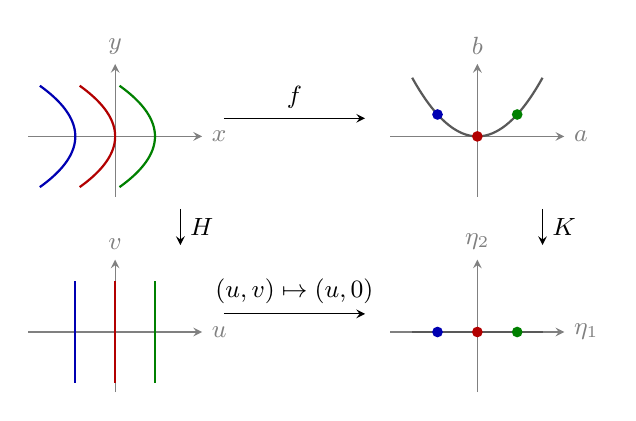
\begin{tikzpicture}[>=stealth,font=\small,scale=.92]
	\begin{scope}[yshift=2.7cm]
		\draw[->,gray] (-1.2,0)--(1.2,0) node[right] {\(x\)};
		\draw[->,gray] (0,-.83)--(0,1) node[above] {\(y\)};
		\foreach \level/\linecolour in {-.55/blue!70!black,0/red!70!black,.55/green!50!black}{
			\draw[thick,\linecolour,domain=-.7:.7,samples=40,variable=\t] plot ({\level-\t*\t},\t);
		}
	\end{scope}
	\begin{scope}[xshift=5cm,yshift=2.7cm]
		\draw[->,gray] (-1.2,0)--(1.2,0) node[right] {\(a\)};
		\draw[->,gray] (0,-.83)--(0,1) node[above] {\(b\)};
		\draw[thick,gray!70!black,domain=-.9:.9,samples=40] plot (\x,{\x*\x});
		\foreach \level/\linecolour in {-.55/blue!70!black,0/red!70!black,.55/green!50!black}{
			\fill[\linecolour] (\level,{\level*\level}) circle (2.1pt);
		}
	\end{scope}
	\draw[->] (1.5,2.95)--(3.45,2.95) node[midway,above] {\(f\)};
	\draw[->] (.9,1.7)--(.9,1.2) node[midway,right] {\(H\)};
	\draw[->] (5.9,1.7)--(5.9,1.2) node[midway,right] {\(K\)};
	\begin{scope}
		\draw[->,gray] (-1.2,0)--(1.2,0) node[right] {\(u\)};
		\draw[->,gray] (0,-.83)--(0,1) node[above] {\(v\)};
		\foreach \level/\linecolour in {-.55/blue!70!black,0/red!70!black,.55/green!50!black}{
			\draw[thick,\linecolour] (\level,-.7)--(\level,.7);
		}
	\end{scope}
	\begin{scope}[xshift=5cm]
		\draw[->,gray] (-1.2,0)--(1.2,0) node[right] {\(\eta_1\)};
		\draw[->,gray] (0,-.83)--(0,1) node[above] {\(\eta_2\)};
		\draw[thick,gray!70!black] (-.9,0)--(.9,0);
		\foreach \level/\linecolour in {-.55/blue!70!black,0/red!70!black,.55/green!50!black}{
			\fill[\linecolour] (\level,0) circle (2.1pt);
		}
	\end{scope}
	\draw[->] (1.5,.25)--(3.45,.25) node[midway,above] {\((u,v)\mapsto(u,0)\)};
\end{tikzpicture}


	\caption[常秩坐标如何同时整理原像与像]{例中的映射 \(f(x,y)=(x+y^2,(x+y^2)^2)\)。上排是原坐标，下排是经 \(H(x,y)=(x+y^2,y)\) 与 \(K(a,b)=(a,b-a^2)\) 改换后的坐标。同色源曲线映到同色目标点；新坐标使各条原像成为竖直线段，使像成为水平直线。图只显示选取的坐标范围。}
	\label{g1:fig:constant-rank-coordinates}
\end{figure}

\begin{corollary}[流形上的常秩标准形]
	\label{g1:cor:manifold-constant-rank}
	设 \(F:M^m\to N^n\) 是无边界光滑流形间的光滑映射，取 \(p\in M\)，且 \(\operatorname{rank}\mathrm{d}F_q=r\) 在 \(p\) 的某个邻域内恒定。则存在 \(p\) 与 \(F(p)\) 附近的光滑坐标，分别以这两点为原点，使 \(F\) 的坐标表达为 \((u^1,\ldots,u^m)\mapsto(u^1,\ldots,u^r,0,\ldots,0)\)，其中末尾有 \(n-r\) 个零，即\eqref{g1:eq:constant-rank-normal-form}。这里不要求坐标变化保持原先给定的度量、长度或角度。
\end{corollary}
\begin{proof}
	先选任意两张坐标图。由\cref{g1:def:manifold-differential,g1:prop:differential-chain-rule}，坐标表达的导数在两侧与坐标微分的可逆线性映射复合，所以它的秩恰为 \(\mathrm{d}F\) 的秩。Euclid 常秩定理给出源、目标坐标域中的进一步微分同胚；将它们与原坐标图复合，仍是光滑坐标图，就得到结论。构造只使用光滑可逆性，未施加任何度量限制。
\end{proof}

\subsection{秩不恒定时的反例}
\label{g1:subsec:1103:04}

常秩假设控制的是一个邻域，不是单点。单点的导数只记录一阶信息，不能独自判定附近原像的形状。不过微分矩阵的连续性确实提供一个有用的单侧结论。

\begin{proposition}
	\label{g1:prop:rank-lower-bound}
	对光滑映射 \(F:M^m\to N^n\)，若 \(\operatorname{rank}\mathrm{d}F_p\geq r\)，则在 \(p\) 的某个邻域中处处有 \(\operatorname{rank}\mathrm{d}F_q\geq r\)。特别地，若在 \(p\) 处秩达到最大可能值 \(\min(m,n)\)，则它在附近自动恒定。
\end{proposition}
\begin{proof}
	在坐标中，秩至少为 \(r>0\) 意味着某个 \(r\) 阶子式非零。该子式是导数矩阵元的多项式，随点连续，所以在足够小邻域中仍非零，秩遂仍至少为 \(r\)。当 \(r=0\) 时结论本身没有限制。最后秩始终不超过 \(\min(m,n)\)，因而达到这一上界时，邻域中的上下界相同。
\end{proof}

\begin{example}
	\label{g1:exm:cubic-rank-change}
	映射 \(f(t)=t^3\) 在原点的导数为零，在其余点的秩为 \(1\)。它仍是 \(\mathbb R\) 到自身的连续双射，逆函数为实立方根；但
	\[
		\frac{f^{-1}(h)-f^{-1}(0)}h=|h|^{-2/3}\longrightarrow\infty
		\qquad(h\to0),
	\]
	所以逆函数在零处不可微。导数可逆是局部光滑可逆的必要条件：若光滑逆存在，对两个复合恒等式求微分，便得到互逆的导数矩阵。它却不是连续可逆的必要条件，立方函数正好区分了这两件事。
\end{example}

在原点把 \(f\) 的秩记为零，并不能将立方函数在邻域中改成常值映射。任意可逆坐标变化都保持每一点的微分秩，而这个例子在任意原点邻域内都有秩为 \(1\) 的点。

\begin{example}
	\label{g1:exm:rank-changing-product}
	考虑 \(F(x,y)=(x,xy)\)，则
	\[
		\mathrm{D}F(x,y)=\begin{pmatrix}1&0\\y&x\end{pmatrix}.
	\]
	它在 \(x\ne0\) 时秩为 \(2\)，在整条 \(x=0\) 的直线上秩为 \(1\)。同值集合也发生明显变化：
	\[
		F^{-1}(a,b)=
		\begin{cases}
			\{(a,b/a)\},&a\ne0,\\
			\{(0,y):y\in\mathbb R\},&(a,b)=(0,0),\\
			\varnothing,&a=0,\ b\ne0.
		\end{cases}
	\]
	尤其在原点附近，整条短竖线被压到一点，旁边的点却各自局部可逆。若源邻域取为 \(|x|<\varepsilon,\ |y|<\delta\)，其像为
	\[
		\{(a,b):0<|a|<\varepsilon,\ |b|<\delta|a|\}\cup\{(0,0)\}.
	\]
	这个像在原点附近既不是开邻域，也不能由一段光滑坐标直线描述。常秩定理证明中的余分量在这里是 \(G(u,v)=uv\)，其 \(\mathrm{D}_vG=u\) 只在 \(u=0\) 上消失，不能因此删掉全部 \(v\) 依赖。
\end{example}

由此可见，若希望一个方程的解集或映射的原像具有稳定的局部维数，必须检查相应邻域中的正则条件。下一节将把满秩情形分别解释为浸入与淹没，并将这些坐标形式用于子流形；本节的结果只处理无边界邻域，半空间边界还需要相应的边界条件。


% !TeX root = ../../Book1.tex
% 纲要标题：### 11.4 浸入、淹没与嵌入
% 纲要位置：几何学计划纲要.md，第 558 行。
% 正文状态：初稿；尚未正式审核。

% 纲要内容开始
% 
% * 浸入和淹没的标准形
% * 正则水平集定理
% * 嵌入、初始子流形结构及限制映射
% * 单射浸入未必嵌入
% * 带边界版本中切空间与边界条件
% 
% ---
% 
% 纲要内容结束

\section{浸入、淹没与嵌入}
\label{g1:sec:1104}

第八章用秩为二的参数映射描述曲面，现在可以把同一个问题放到任意维数的流形上。一张参数片是否丢失切向方向，由微分是否单射判断；一个方程组能否在附近独立控制所有输出，由微分是否满射判断。但即使每张参数片都很规整，远处的参数仍可能回到眼前，这就需要另加拓扑条件。常秩定理先给出局部图像，嵌入的定义再保证这些局部图像与整个像的拓扑相符。本节前四个小节先讨论无边界流形，最后专门说明边界处哪些条件需要补充。

\subsection{浸入和淹没的标准形}
\label{g1:subsec:1104:01}

\begin{definition}[浸入与淹没]\label{g1:def:immersion-submersion}
	设 \(F:M^m\to N^n\) 是光滑映射。若 \(\mathrm{d}F_p:\mathrm{T}_pM\to \mathrm{T}_{F(p)}N\) 单射，称 \(F\) 在 \(p\) 处为浸入；若它满射，称 \(F\) 在 \(p\) 处为\term[yanmo]{淹没}[submersion]。处处满足相应条件时，分别称 \(F\) 为浸入或淹没。
\end{definition}

这里的浸入推广了\cref{g1:def:surface-immersion}中的曲面参数：其定义域维数为二，所以满列秩正是两个参数方向不被压在一起。一般浸入必须有 \(m\le n\)，一般淹没必须有 \(m\ge n\)。淹没也不要求映射在集合意义下满射，例如 \(t\mapsto e^t\) 是 \(\mathbb R\to\mathbb R\) 的淹没，而像只是正半轴。

\begin{theorem}[浸入与淹没的局部标准形]\label{g1:thm:immersion-submersion-normal-form}
	设 \(M^m,N^n\) 是无边界光滑流形，\(F:M\to N\) 光滑，\(p\in M\)。
	\begin{enumerate}
		\item 若 \(\mathrm{d}F_p\) 单射，则存在分别以 \(p,F(p)\) 为原点的源、目标坐标，使 \(F\) 在源的一个邻域中写成
		\[
			(u^1,\ldots,u^m)\longmapsto(u^1,\ldots,u^m,0,\ldots,0).
		\]
		\item 若 \(\mathrm{d}F_p\) 满射，则可选这样的坐标，使 \(F\) 写成
		\[
			(u^1,\ldots,u^m)\longmapsto(u^1,\ldots,u^n).
		\]
	\end{enumerate}
\end{theorem}
\begin{proof}
	单射情形，坐标 Jacobian 在 \(p\) 处有一个非零的 \(m\) 阶子式，连续性使它在某邻域内仍非零。秩又不能超过源维数 \(m\)，故该邻域的秩恒为 \(m\)。满射情形同理：一个非零的 \(n\) 阶子式保证邻域内的秩恒为 \(n\)。现在分别对秩 \(m\) 和秩 \(n\) 使用\cref{g1:cor:manifold-constant-rank}，就得到两种标准形。这里先证明邻域内秩恒定，才能调用常秩结论；仅知道一点的非极大秩，通常不能这样做。
\end{proof}

从标准形可以读出两项常用结论。浸入限制到足够小的源邻域后，是到其像的同胚：在坐标中只需投影到前 \(m\) 个坐标就得到连续逆映射。这说的是一个指定的参数分支，并没有断言其他参数分支不会进入同一个目标邻域。

\ProseParagraphBreak

无边界流形之间的淹没是开映射。事实上，把任一源开集中的点放进包含在该开集内的坐标小盒，投影标准形把这个小盒送到目标中的开盒，所有这些像的并就是原开集的像。此外，若 \(q=F(p)\)，在投影标准形中取被忘掉的坐标恒为零，就得到一个通过 \(p\) 的光滑局部截面 \(s\)，满足 \(F\circ s=\operatorname{id}\)。因此淹没允许在目标点附近光滑选择一个原像，但未必能把这些局部选择拼成全局截面。

\subsection{正则水平集定理}
\label{g1:subsec:1104:02}

方程 \(F(p)=y\) 应当减少多少自由度，取决于它实际提供了多少个独立约束。若目标维数为 \(n\)，微分满射正是所有 \(n\) 个约束在一阶上独立。淹没标准形将这个判断直接变成坐标中固定前 \(n\) 个数。

\begin{definition}[正则值]\label{g1:def:regular-value}
	设 \(F:M\to N\) 光滑。若 \(\mathrm{d}F_p\) 满射，称 \(p\) 为 \(F\) 的\term[zhengzedian]{正则点}[regular point]；否则称为\term[linjiedian]{临界点}[critical point]。若 \(y\in N\) 的每个原像都是正则点，称 \(y\) 为\term[zhengzezhi]{正则值}[regular value]；否则称为\term[linjiezhi]{临界值}[critical value]。没有原像的点也按此定义算作正则值。
\end{definition}

\begin{theorem}[正则水平集]\label{g1:thm:regular-level-set}
	设 \(F:M^m\to N^n\) 是无边界光滑流形之间的光滑映射，\(y\in N\) 是正则值。若 \(S=F^{-1}(y)\) 非空，则 \(S\) 在子空间拓扑下有自然的 \((m-n)\) 维光滑流形结构，包含映射 \(i:S\hookrightarrow M\) 是浸入，且
	\begin{equation}\label{g1:eq:regular-level-tangent}
		\mathrm{d}i_p(\mathrm{T}_pS)=\ker\mathrm{d}F_p\qquad(p\in S).
	\end{equation}
	通过单射 \(\mathrm{d}i_p\) 把 \(\mathrm{T}_pS\) 视为 \(\mathrm{T}_pM\) 的子空间时，可简写为 \(\mathrm{T}_pS=\ker\mathrm{d}F_p\)。
\end{theorem}
\begin{proof}
	对每个 \(p\in S\) 使用淹没标准形，将 \(y\) 的目标坐标取为零。在所得源坐标 \((u^1,\ldots,u^m)\) 中，水平集恰为
	\[
		u^1=\cdots=u^n=0.
	\]
	因此后 \(m-n\) 个坐标给出 \(S\) 的局部坐标，而且这些坐标与 \(S\) 的子空间拓扑一致。两张这样的坐标之间，转换映射是在环境坐标转换中先代入前 \(n\) 个坐标为零，再取所需坐标分量，故光滑；逆转换同理。这构成光滑图册。Hausdorff 性和第二可数性从环境的子空间继承，所以确实得到流形。

	在这些坐标中，包含映射的微分把后 \(m-n\) 个坐标方向单射送入 \(\mathrm{T}_pM\)。另一方面，\(\mathrm{d}F_p\) 是前 \(n\) 个方向的投影，其核恰由后 \(m-n\) 个方向张成。于是得到\eqref{g1:eq:regular-level-tangent}。坐标改变通过\cref{g1:prop:differential-chain-rule}的微分链式法则相容，所以这个子空间描述不依赖所选坐标。
\end{proof}

下一小节将通过包含映射的性质进一步说明这个自然结构为何唯一。这里并非随意给同一集合指定一种流形拓扑。只需在水平集各点满足正则值的条件，不要求 \(F\) 在整个 \(M\) 上都是淹没。

\begin{example}\label{g1:exm:regular-sphere-and-singular-level}
	设 \(F:\mathbb R^{k+1}\to\mathbb R\)，\(F(x)=\|x\|^2\)，其中 \(k\ge1\)。因为
	\[
		\mathrm{d}F_x(v)=2\langle x,v\rangle,
	\]
	每个 \(c>0\) 都是正则值，球面 \(F^{-1}(c)\) 的维数为 \(k\)，并且 \(\mathrm{T}_xF^{-1}(c)=x^\perp\)。负数也为正则值，但水平集为空。零为临界值，其水平集只有一个点；该集合仍可以是零维流形，却不具有正则水平集定理所给的预期维数 \(k\)。

	另取 \(G(x,y)=xy\)。它的零水平集是两条坐标轴的并，在原点形成四条分支，不是原点附近的一维流形。两个例子说明：临界水平集有时仍规整，有时出现交叉，仅由“不是正则值”不能断言所有水平集具有同一种奇异性。
\end{example}

\subsection{嵌入、初始子流形结构及限制映射}
\label{g1:subsec:1104:03}

第四章的拓扑嵌入要求映射与其像之间互为连续逆映射，像必须使用环境的子空间拓扑。加入这个条件以后，浸入的局部参数片才会与整个像的局部邻域一致。

\begin{definition}[光滑嵌入]\label{g1:def:smooth-embedding}
	无边界光滑流形之间的光滑映射 \(f:M\to N\)，若既是浸入，又是 \(M\) 到 \(f(M)\) 的同胚，其中 \(f(M)\) 取 \(N\) 的子空间拓扑，则称为\term[guanghuaqianru]{光滑嵌入}[smooth embedding]，简称嵌入。
\end{definition}

\begin{definition}[嵌入子流形]\label{g1:def:embedded-submanifold}
	设 \(N^n\) 为无边界光滑流形。子集 \(S\subset N\) 若对每个 \(p\in S\) 都有环境坐标 \((V,y)\)，使
	\[
		y(S\cap V)=y(V)\cap\bigl(\mathbb R^k\times\{0\}^{n-k}\bigr),
	\]
	则称为 \(N\) 的 \(k\) 维\term[qianruziliuxing]{嵌入子流形}[embedded submanifold]。给 \(S\) 子空间拓扑，并用这些切片的前 \(k\) 个坐标作为图册。
\end{definition}

坐标切片之间的转换正如正则水平集证明中那样光滑，所以这个定义确实给出 \(S\) 的光滑结构。下述等价关系说明，这个集合式定义与前面的映射式定义对应。

\begin{proposition}[嵌入与坐标切片]\label{g1:prop:embedding-slice-characterization}
	设 \(M^k,N^n\) 是无边界光滑流形。若 \(f:M\to N\) 为光滑嵌入，则其像 \(S=f(M)\) 为嵌入子流形，且 \(f:M\to S\) 是微分同胚。反之，每个嵌入子流形的包含映射都是光滑嵌入。
\end{proposition}
\begin{proof}
	取 \(p\in M\)，浸入标准形给出源邻域 \(U\) 及 \(f(p)\) 附近的坐标，使 \(f|_U\) 的像是一块坐标切片。必要时缩小坐标盒，可以使这块切片完整覆盖目标小盒中的前 \(k\) 个坐标。关键是排除 \(M\setminus U\) 的点也映入眼前的小盒：因为 \(f\) 是到子空间 \(S\) 的同胚，\(f(U)\) 在 \(S\) 中开，故存在环境开集 \(W\subset N\)，满足 \(S\cap W=f(U)\)。把目标坐标盒进一步缩到 \(W\) 内，盒内的整个 \(S\) 就恰为该切片，而不只是其中一个参数分支。这样的盒覆盖 \(S\)，给出嵌入子流形结构。在对应坐标中，\(f:M\to S\) 是恒等坐标映射，故连同逆映射都光滑。

	反过来，包含映射在适配坐标中为 \(u\mapsto(u,0)\)，所以是浸入。\(S\) 已取环境的子空间拓扑，包含映射自然是到其像的同胚，故为光滑嵌入。
\end{proof}

\begin{proposition}[嵌入子流形的初始性质]\label{g1:prop:embedded-initial-property}
	设 \(S\subset N\) 为无边界光滑流形 \(N\) 的嵌入子流形，\(i:S\hookrightarrow N\) 为包含映射。对任意光滑流形 \(P\)（允许有边界）及任意集合映射 \(h:P\to S\)，有
	\[
		h:P\to S\text{ 光滑}\quad\Longleftrightarrow\quad i\circ h:P\to N\text{ 光滑}.
	\]
	特别地，光滑映射 \(H:P\to N\) 若像包含在 \(S\) 中，就唯一地给出光滑映射 \(P\to S\)。在固定子集 \(S\subset N\) 上，使其成为嵌入子流形的光滑结构唯一。
\end{proposition}
\begin{proof}
	正向由光滑映射的复合得到。反向先处理一个容易遗漏的拓扑问题：若 \(i\circ h\) 光滑，则它连续；由于 \(S\) 取子空间拓扑，\(h\) 也连续。于是对 \(h(p)\) 附近的适配图 \(V\)，集合 \(h^{-1}(S\cap V)\) 在 \(P\) 中开。在这片上，\(h\) 的坐标表示就是 \(i\circ h\) 的坐标表示的前 \(\dim S\) 个分量，所以光滑。即使 \(p\) 在 \(\partial P\)，这些分量仍由环境中的光滑延拓限制得到，论证不变。局部结论合起来给出 \(h\) 光滑。

	像包含在 \(S\) 的映射只有一种集合意义下的限制值域方式，上述等价立即证明其光滑性。若同一个子集带有两种嵌入子流形结构，两种包含映射都光滑。对两种结构之间的恒等集合映射分别使用已证等价，得到恒等映射在两个方向都光滑，故两种极大光滑图册相同。
\end{proof}

这里的“初始”说的是通过包含映射检测光滑性的性质，不是另给 \(S\) 加一种比子空间拓扑更细的拓扑。例如光滑函数 \(f:N\to\mathbb R\) 限制到 \(S\) 后光滑；若 \(f(S)\subset T\)，其中 \(T\) 也是嵌入子流形，则 \(f|_S:S\to T\) 光滑。正则水平集由环境坐标切片构造，因而属于这一情形。

\ProseParagraphBreak

包含映射的微分通常被省略在记号里：对嵌入子流形写 \(\mathrm{T}_pS\subset \mathrm{T}_pN\)，实际是用单射 \(\mathrm{d}i_p\) 作识别。这不是把两个定义不同的导子集合逐项当作相同集合，而是利用包含映射，在前者与后者的一个子空间之间建立自然的线性同构。

\subsection{单射浸入未必嵌入}
\label{g1:subsec:1104:04}

单射解决了“一个像点有几个原像”，却没有解决“附近像点的原像是否也在附近”。下面的平面曲线已经能把两者区别开，不需要依靠高维或稠密轨道的例子。

\begin{example}\label{g1:exm:injective-immersion-not-embedding}
	令
	\[
		\gamma:(-\pi,\pi)\longrightarrow\mathbb R^2,
		\qquad\gamma(t)=(\sin t,\sin2t).
	\]
	它是单射浸入，但不是嵌入。先检查浸入：\(\gamma'(t)=(\cos t,2\cos2t)\)，若第一分量为零，则 \(t=\pm\pi/2\)，第二分量为 \(-2\ne0\)，故导数从不为零。

	再检查单射。\(\sin t\) 的正负区分正、负参数，且在本区间内只在 \(t=0\) 为零。若 \(s,t\in(0,\pi)\) 且 \(\sin s=\sin t\)，则 \(s=t\) 或 \(s=\pi-t\)；后一情形的 \(\sin2s=-\sin2t\)，两者相等只能有 \(t=\pi/2\)，此时仍为 \(s=t\)。负参数的情形用 \(\gamma(-t)=-\gamma(t)\) 化为正参数，因而 \(\gamma\) 单射。

	然而取 \(t_j\to\pi\)，便有 \(\gamma(t_j)\to(0,0)=\gamma(0)\)，而 \(t_j\) 不趋于零。因此从像的子空间拓扑返回参数的逆映射不连续。\cref{g1:fig:injective-immersion-topology}中，蓝色短弧来自零附近的参数，另一方向逼近交点的曲线来自接近参数区间端点的部分。浸入标准形只能控制前一支。

	这个像甚至是闭集：把同一公式延拓到紧区间 \([-\pi,\pi]\)，两个端点都映到已有的 \(\gamma(0)\)，所以延拓前后的像相同，是紧集。可见“单射浸入且像闭”仍不能替代嵌入条件。
\end{example}

% !TeX root = ../Book1.tex
\begin{figure}[htbp]
	\centering
	\begin{tikzpicture}[font=\small]
		\begin{scope}[xshift=-2.8cm,x=2cm,y=1.3cm]
			\draw[->,GeometryGray] (-1.25,0)--(1.3,0) node[right] {\(x\)};
			\draw[->,GeometryGray] (0,-1.2)--(0,1.25) node[above] {\(y\)};
			\draw[GeometryGray,thick,domain=-180:180,samples=181,variable=\t] plot ({sin(\t)},{sin(2*\t)});
			\draw[GeometryBlue,very thick,domain=-27:27,samples=40,variable=\t] plot ({sin(\t)},{sin(2*\t)});
			\draw[orange!75!black,very thick,domain=145:179.8,samples=35,variable=\t] plot ({sin(\t)},{sin(2*\t)});
			\foreach \t in {150,165,174,178}{\fill[orange!75!black] ({sin(\t)},{sin(2*\t)}) circle (1.25pt);}
			\fill[GeometryBlue] (0,0) circle (1.6pt);
			\node[above left] at (0,0) {\(\gamma(0)\)};
			\node[GeometryBlue,above right] at (0.5,0.78) {\(t\approx0\)};
			\node[orange!75!black,right] at (0.63,-0.72) {\(t\uparrow\pi\)};
		\end{scope}
		\begin{scope}[xshift=3.7cm,yshift=0.2cm]
			\draw[GeometryGray] (-1.7,0)--(1.7,0);
			\draw[fill=white] (-1.7,0) circle (2pt);
			\draw[fill=white] (1.7,0) circle (2pt);
			\fill[GeometryBlue] (0,0) circle (2pt);
			\node[below] at (-1.7,0) {\(-\pi\)};
			\node[below] at (0,0) {\(0\)};
			\node[below] at (1.7,0) {\(\pi\)};
			\foreach \x in {1,1.35,1.52,1.61}{\fill[orange!75!black] (\x,0) circle (1.5pt);}
			\draw[->,orange!75!black] (0.95,0.35)--(1.65,0.35);
			\node[above] at (0,0.75) {参数区间 \((-\pi,\pi)\)};
			\node[align=center] at (0,-1) {\(\gamma(t_j)\to\gamma(0)\)\\但 \(t_j\not\to0\)};
		\end{scope}
	\end{tikzpicture}
	\caption[单射浸入的像拓扑]{曲线 \(\gamma(t)=(\sin t,\sin2t)\)，定义域为 \((-\pi,\pi)\)。蓝色弧是零附近的参数片；橙色点来自趋向 \(\pi\) 的参数，也在像中趋向原点。逆参数映射因而不连续，尽管每个参数点的导数非零且参数映射单射。}
	\label{g1:fig:injective-immersion-topology}
\end{figure}


还可以在这个例子中具体看出，嵌入子流形的初始性质不能自动移植给任意单射浸入像。给集合 \(S=\gamma((-\pi,\pi))\) 从参数区间搬来流形结构，使 \(\gamma\) 成为微分同胚；此时包含 \(S\to\mathbb R^2\) 是浸入。对充分小的 \(\varepsilon>0\)，考虑值在 \(S\) 中的曲线
\[
	h(s)=(-\sin s,\sin2s),\qquad |s|<\varepsilon.
\]
作为到 \(\mathbb R^2\) 的映射，它光滑；但它在 \(S\) 的参数坐标为
\[
	\gamma^{-1}(h(s))=
	\begin{cases}
		\pi+s,&s<0,\\
		0,&s=0,\\
		-\pi+s,&s>0,
	\end{cases}
\]
在零处不连续，故 \(h:(-\varepsilon,\varepsilon)\to S\) 不是光滑映射。问题恰是这份流形结构的拓扑不同于 \(S\) 的子空间拓扑。

\begin{definition}[固有映射]\label{g1:def:proper-map-manifolds}
	光滑流形之间的连续映射 \(f:M\to N\) 若对每个紧集 \(K\subset N\)，原像 \(f^{-1}(K)\) 都紧，则称为\term[guyouyingshe]{固有映射}[proper map]。
\end{definition}

固有性控制的是“落在一个固定紧目标区域内的所有参数”。上一例中整个像紧，而其原像是非紧区间 \((-\pi,\pi)\)，所以 \(\gamma\) 不固有。这一条件能排除远处参数悄悄回到紧区域的现象。

\begin{proposition}[固有单射浸入]\label{g1:prop:proper-injective-immersion}
	设 \(M,N\) 为无边界光滑流形，\(f:M\to N\) 为单射浸入。若 \(f\) 固有，则 \(f\) 是嵌入，且像闭于 \(N\)。特别地，若 \(M\) 紧，则每个单射浸入 \(M\to N\) 都是闭像嵌入。反之，闭像嵌入是固有映射。
\end{proposition}
\begin{proof}
	先证明一个连续固有映射 \(f:M\to N\) 是闭映射。取闭集 \(A\subset M\) 及 \(y\in\overline{f(A)}\)。在 \(N\) 的坐标图内取一个紧邻域 \(K\ni y\)，使 \(y\in\operatorname{int}K\)。固有性使 \(f^{-1}(K)\) 紧，故其闭子集 \(A\cap f^{-1}(K)\) 紧。它的连续像
	\[
		f(A\cap f^{-1}(K))=f(A)\cap K
	\]
	也紧，并由\cref{g1:prop:compact-hausdorff-closed}闭于 \(N\)。回忆这里闭性的理由：对紧集外一点，用 Hausdorff 性把它与紧集的每一点用开邻域分开，再以有限子覆盖替代紧集一侧的全部邻域，取外点一侧有限个邻域的交，便得到与紧集不交的开邻域。因为 \(y\) 位于 \(K\) 的内部且是 \(f(A)\) 的闭包点，它也是 \(f(A)\cap K\) 的闭包点，因而属于该闭集。于是 \(f(A)\) 闭。

	现在 \(f\) 连续且单射，并将闭集送到闭集，所以 \(f:M\to f(M)\) 的逆映射连续。它又是浸入，故为嵌入；取 \(A=M\) 还得到像闭。若 \(M\) 紧，每个目标紧集在 Hausdorff 空间 \(N\) 中闭，其原像为 \(M\) 的闭子集，因而紧，所以 \(f\) 自动固有。此时也可直接使用\cref{g1:thm:compact-bijection}判断到像的逆连续。

	反之，若 \(f\) 是闭像嵌入，则 \(K\cap f(M)\) 对每个紧 \(K\subset N\) 都是紧集；由同胚 \(M\cong f(M)\)，其原像 \(f^{-1}(K)\) 紧，故 \(f\) 固有。
\end{proof}

并非所有嵌入都固有。例如开区间 \((0,1)\hookrightarrow\mathbb R\) 是嵌入，但紧集 \([0,1]\) 的原像不紧。固有单射浸入给出的是一种保证闭像嵌入的充分判据，并没有把“嵌入”的含义改成“闭子集”。

\subsection{带边界版本中切空间与边界条件}
\label{g1:subsec:1104:05}

对带边界流形，浸入、淹没仍按完整微分的单射、满射定义，嵌入仍要求同时是浸入和到子空间像的同胚。边界坐标采用 \(\mathbb H^m=\{x^m\ge0\}\)。\cref{g1:prop:derivation-coordinate-basis}及\cref{g1:prop:boundary-velocities}说明，即使 \(p\in\partial M\)，完整切空间 \(\mathrm{T}_pM\) 仍是 \(m\) 维向量空间；向内半空间只是其中能够由向内单侧曲线实现的速度集合，不能代替整个切空间。若以 \(\rho=x^m\) 为局部边界定义函数，则
\[
	\mathrm{T}_p(\partial M)=\ker\mathrm{d}\rho_p\subset \mathrm{T}_pM.
\]
边界上各种满秩条件因此仍按完整切空间计算，但由此得到的 Euclid 局部变换未必保留半空间。

\begin{proposition}[边界处的局部逆]\label{g1:prop:boundary-local-inverse}
	设 \(M^m,N^m\) 为带边界光滑流形，\(m\ge1\)，\(F:M\to N\) 光滑。若 \(p\in\partial M\)、\(F(p)\in\partial N\)，在 \(p\) 的某邻域内有 \(F(\partial M)\subset\partial N\)，并且 \(\mathrm{d}F_p\) 可逆，则 \(F\) 限制到 \(p\) 的某个相对开邻域后，是到 \(F(p)\) 的一个相对开邻域的微分同胚。
\end{proposition}
\begin{proof}
	取两边的半空间坐标，把 \(p,F(p)\) 都置于零。按边界光滑映射的定义，坐标表示 \(G\) 可光滑延拓到 \(\mathbb R^m\) 的一个开邻域。保边界条件给出 \(G^m(x',0)=0\)，所以由一元微积分基本定理，
	\[
		G^m(x',x^m)=x^m a(x',x^m),\qquad
		a(x',x^m)=\int_0^1\partial_mG^m(x',t x^m)\,\mathrm{d}t.
	\]
	\(\mathrm{d}G_0\) 的最后一行在前 \(m-1\) 列为零；可逆性因而使 \(a(0)\ne0\)。又因为 \(G\) 把 \(x^m\ge0\) 的点送到目标半空间，一侧导数给出 \(a(0)\ge0\)，故 \(a(0)>0\)。缩小邻域使 \(a>0\)，则 \(G^m\) 与 \(x^m\) 同号。对 Euclid 延拓使用\cref{g1:thm:inverse-function}，得到开邻域间的光滑逆；同号性质说明该逆也保留半空间。把这对互逆映射限制到半空间，便得到所需边界局部逆。
\end{proof}

保边界条件不能只检查在一个点成立。例如
\[
	G:\mathbb H^2\to\mathbb H^2,\qquad G(x,y)=(x,y+x^2)
\]
在原点的微分是恒等映射，也把原点送到原点，但它把附近的边界点送到抛物线 \(v=u^2\)。其像在 \(v\ge u^2\) 中，不包含原点在目标半平面中的任何相对开邻域，所以不是边界局部微分同胚。Euclid 延拓的逆 \((u,v)\mapsto(u,v-u^2)\) 光滑，却未必取值于源半平面。

\ProseParagraphBreak

对水平集，正确的附加条件要求约束在边界切向方向中仍然独立。这样，约束不会把唯一的向内方向全部吃掉。若带边界子流形 \(S\subset M\) 满足 \(\partial S=S\cap\partial M\)，且在这些点满足
\[
	\mathrm{T}_pS+\mathrm{T}_p(\partial M)=\mathrm{T}_pM,
\]
本书用\term[neatziliuxing]{与边界相容的横截嵌入子流形}[neat submanifold]描述同时满足这两个条件的子流形。这里包含映射要求为嵌入；横截等式意味着 \(\mathrm{T}_pS\) 中还保留至少一个不沿环境边界的方向。

\begin{theorem}[带边界的正则水平集]\label{g1:thm:boundary-regular-level-set}
	设 \(M^m\) 为带边界光滑流形，\(N^n\) 为无边界光滑流形，\(F:M\to N\) 光滑。若 \(y\in N\) 同时为 \(F\) 及 \(F|_{\partial M}\) 的正则值，则非空水平集 \(S=F^{-1}(y)\) 自然成为 \((m-n)\) 维带边界嵌入子流形，且
	\[
		\partial S=S\cap\partial M,\qquad \mathrm{T}_pS=\ker\mathrm{d}F_p.
	\]
	它是与边界相容的横截嵌入子流形；在边界点还满足
	\[
		\mathrm{T}_p(\partial S)=\ker\mathrm{d}F_p\cap \mathrm{T}_p(\partial M).
	\]
\end{theorem}
\begin{proof}
	内部点使用\cref{g1:thm:regular-level-set}的局部证明。取 \(p\in S\cap\partial M\)，用半空间坐标将 \(p\) 置于零，用目标坐标将 \(y\) 置于零，记映射的坐标分量为 \(f^1,\ldots,f^n\)。\(F|_{\partial M}\) 在 \(p\) 处满秩，意味着 Jacobian 的前 \(m-1\) 列中有一个非零的 \(n\) 阶子式。重排前 \(m-1\) 个坐标，可令该子式来自前 \(n\) 列。特别地，若水平集碰到边界，必有 \(m-n\ge1\)。

	对 \(f\) 的 Euclid 光滑延拓构造
	\[
		\Phi(x)=\bigl(f^1(x),\ldots,f^n(x),x^{n+1},\ldots,x^{m-1},x^m\bigr).
	\]
	\(\mathrm{d}\Phi_0\) 可逆，故由\cref{g1:thm:inverse-function}，它在足够小的 Euclid 开邻域间为微分同胚。与任意使用常秩定理不同，这里特意把最后一个坐标原样保留：\(\Phi^m(x)=x^m\)。因此 \(\Phi\) 及其逆都保留半空间和边界。以 \(u=\Phi(x)\) 为新的边界坐标，水平集成为
	\begin{equation}\label{g1:eq:boundary-level-slice}
		u^1=\cdots=u^n=0,\qquad u^m\ge0.
	\end{equation}
	后 \(m-n\) 个坐标给出水平集的半空间图，其边界恰是 \(u^m=0\)，也就是环境边界与水平集的交。图册转换由环境光滑转换的限制得到，子空间拓扑、Hausdorff 性及第二可数性同无边界情形，因此得到带边界嵌入子流形。

	在这些坐标中，\(\mathrm{T}_pS\) 由后 \(m-n\) 个完整坐标方向张成，等于 \(\ker\mathrm{d}F_p\)；其边界切空间再去掉最后一个方向，正是 \(\ker\mathrm{d}F_p\cap \mathrm{T}_p(\partial M)\)。最后一个方向 \(\partial/\partial u^m\) 属于 \(\mathrm{T}_pS\) 却不属于 \(\mathrm{T}_p(\partial M)\)，而后者余维为一，故两者之和为整个 \(\mathrm{T}_pM\)。这就同时验证了边界交等式与横截条件。
\end{proof}

上述半空间切片还说明，与边界相容的横截水平集仍具有初始性质：一个映射若值在 \(S\) 中，其是否光滑可以通过组合包含 \(S\hookrightarrow M\) 来检验。证明仍先用子空间拓扑得到连续性，再取\eqref{g1:eq:boundary-level-slice}中后 \(m-n\) 个坐标；这些坐标有环境光滑延拓，因此同样适用于带边界的源。

\ProseParagraphBreak

只检查完整切空间上的 \(\mathrm{d}F\) 满射还不够。例如 \(F:\mathbb H^m\to\mathbb R\)，\(F(x)=x^m\)，处处满秩，但 \(F^{-1}(0)=\partial M\) 是一张无边界的 \((m-1)\) 维流形；其自身边界为空，而与 \(\partial M\) 的交却是整个水平集，故不是 与边界相容的横截水平集。更明显地，\(F(x,y)=y+x^2\) 在 \(\mathbb H^2\) 上也处处满秩，但零水平集只有原点，连预期的一维局部形状都没有。两例中 \(F|_{\partial M}\) 都在相关点失去满秩性，正是附加条件所要排除的现象。


\begin{chaptersummary}
	光滑结构由两两相容的坐标图确定，坐标图的极大扩张消除了任意多列或少列相容图的区别。球面和射影空间可以直接用图册构造；同一个底层拓扑却不能独自决定哪些函数光滑。边界图使用半空间中的局部延拓，延拓函数可以不同，但边界点处各阶导数相同。

	\ProseParagraphBreak

	切向量是作用于局部函数芽的一阶导子，坐标导数给出它的基。内点处每个切向量都能由双侧曲线实现；边界处双侧速度只给出边界切空间，单侧速度给出内向锥，完整切空间仍为 \(n\) 维。切丛把不同点的切空间通过微分换坐标组织在一起；光滑映射的微分向前送切向量，其对偶反向拉回余切向量。

	\ProseParagraphBreak

	逆函数定理以可逆线性近似控制非线性余项，通过压缩迭代产生局部逆。隐函数定理把待求变量与参数一起放入这一构造；常秩定理再利用秩在邻域中不变，消去剩余坐标的变化，得到局部投影或坐标包含。满秩约束因此给出光滑水平集，切空间正是约束微分的核。

	\ProseParagraphBreak

	浸入只控制局部切方向，嵌入还要求源拓扑与像的子空间拓扑相符；单射和闭像各自都不足以代替这一条件，固有性则提供实用的充分条件。边界问题还必须辨认边界是否对应、约束是否沿边界仍满秩。Euclid 延拓的局部可逆，不会自动保证它的逆留在所需的半空间一侧。
\end{chaptersummary}

\BookExercises


\begin{exercise}
	\label{g1:ex:stereographic-smooth-charts}
	设 \(n\geq1\)，\(N=(0,\ldots,0,1)\)、\(S=-N\) 是 \(S^n\) 的两极。对 \(x=(x',x_{n+1})\) 定义
	\[
		\sigma_N(x)=\frac{x'}{1-x_{n+1}},\qquad
		\sigma_S(x)=\frac{x'}{1+x_{n+1}}.
	\]
	求这两个映射的逆，证明它们给出与\cref{g1:exm:sphere-smooth-atlas}相同的光滑结构，并求换坐标 \(\sigma_S\circ\sigma_N^{-1}\)。说明换坐标在零点没有定义的几何原因。
\end{exercise}

\begin{solution}
	解 \(u=x'/(1-x_{n+1})\) 与 \(|x'|^2+x_{n+1}^2=1\)，得到
	\[
		\sigma_N^{-1}(u)=\left(\frac{2u}{1+|u|^2},\frac{|u|^2-1}{1+|u|^2}\right),\qquad
		\sigma_S^{-1}(v)=\left(\frac{2v}{1+|v|^2},\frac{1-|v|^2}{1+|v|^2}\right).
	\]
	这些式子对任意 \(u,v\in\mathbb R^n\) 有意义，代回即得到恒等式，且与原映射均连续。因此它们分别是 \(S^n\setminus\{N\}\)、\(S^n\setminus\{S\}\) 到 \(\mathbb R^n\) 的坐标图。与正文半球图转换时，一向由上述有理式后删除一个分量得到，另一向由半球图的光滑平方根表达代入 \(\sigma_N\) 或 \(\sigma_S\) 得到，分母在相应交叠处非零，故两种图册相容。

	在 \(u\neq0\) 时，把逆式代入可得
	\[
		(\sigma_S\circ\sigma_N^{-1})(u)=\frac{u}{|u|^2}.
	\]
	该映射的逆仍是自身。\(u=0\) 在北极投影图中代表南极，而南极不属于另一张图的图域，故这里的未定义来自图域没有交叠，并非球面的奇点。
\end{solution}

\begin{exercise}
	\label{g1:ex:projective-line-circle}
	证明映射
	\[
		F:\mathbb{RP}^1\longrightarrow S^1,\qquad
		F([x:y])=\left(\frac{x^2-y^2}{x^2+y^2},\frac{2xy}{x^2+y^2}\right)
	\]
	是微分同胚。要求直接给出局部逆的坐标公式，不只利用紧空间到 Hausdorff 空间的连续双射性质。
\end{exercise}

\begin{solution}
	两个分式在同时缩放 \((x,y)\) 后不变，且其平方和为 \(1\)，所以 \(F\) 良定义。在图 \(x\neq0\) 中写 \(t=y/x\)，有
	\[
		F([1:t])=\left(\frac{1-t^2}{1+t^2},\frac{2t}{1+t^2}\right).
	\]
	它的像为圆周除去 \((-1,0)\)，逆坐标为 \(t=b/(1+a)\)，其中 \((a,b)\in S^1\)、\(a\neq-1\)。在图 \(y\neq0\) 中写 \(s=x/y\)，得到
	\[
		F([s:1])=\left(\frac{s^2-1}{s^2+1},\frac{2s}{s^2+1}\right),\qquad s=\frac{b}{1-a}\quad(a\neq1).
	\]
	两组逆式覆盖整个圆周。在同时有定义处，\(st=b^2/((1-a)(1+a))=1\)，所以它们给出同一射影点。两组公式还证明满射与单射；正文的球面图与射影图中各式都光滑，因此 \(F\) 及其逆光滑。
\end{solution}

\begin{exercise}
	\label{g1:ex:transported-line-powers}
	对正奇数 \(r\)，在通常拓扑的 \(\mathbb R\) 上用全局坐标 \(u_r(t)=t^r\) 定义光滑流形 \(M_r\)。对两个正奇数 \(r,s\)，判断集合恒等映射 \(I_{r,s}:M_r\to M_s\) 何时光滑、何时为微分同胚。证明无论 \(r,s\) 如何，\(M_r\) 与 \(M_s\) 总微分同胚。
\end{exercise}

\begin{solution}
	恒等映射的坐标表达为 \(u\mapsto\operatorname{sgn}(u)|u|^{s/r}\)。若 \(s/r\) 是整数，由 \(r,s\) 都为奇数知它是正奇数，表达式就是光滑多项式 \(u^{s/r}\)。若 \(\alpha=s/r\) 不是整数，取 \(k=\lfloor\alpha\rfloor+1\)，在正半轴上第 \(k\) 阶导数等于非零常数乘 \(u^{\alpha-k}\)，当 \(u\downarrow0\) 时无界，因此不可能在零点 \(C^k\)，更不光滑。故 \(I_{r,s}\) 光滑当且仅当 \(r\) 整除 \(s\)；正反两个恒等映射同时光滑当且仅当 \(r=s\)。

	不过映射 \(F=u_s^{-1}\circ u_r:M_r\to M_s\) 始终是微分同胚，因为 \(u_s\circ F\circ u_r^{-1}\) 为恒等映射，逆也一样。具体集合公式为 \(F(t)=\operatorname{sgn}(t)|t|^{r/s}\)。这个公式在通常坐标中可能不光滑，并不妨碍它在指定的源、目标结构之间成为微分同胚。
\end{solution}

\begin{exercise}
	\label{g1:ex:boundary-even-extension}
	设 \(f:[0,\infty)\to\mathbb R\) 按局部延拓意义光滑。证明偶延拓 \(E_f(t)=f(|t|)\) 在 \(\mathbb R\) 上光滑，当且仅当 \(f^{(2j+1)}(0)=0\) 对所有 \(j\geq0\) 成立。再构造一个在负半轴不恒为零的光滑函数 \(h:\mathbb R\to\mathbb R\)，使 \(h\) 在非负半轴恒为零，解释为什么边界处各阶导数的唯一性不意味着延拓函数唯一。
\end{exercise}

\begin{solution}
	如果 \(E_f\) 光滑，由它是偶函数可得 \(E_f^{(k)}(0)=(-1)^kE_f^{(k)}(0)\)，故所有奇阶导数为零；在右侧这些导数就是 \(f\) 的边界导数。

	反过来，假设所有奇阶边界导数为零。在正、负半轴上，\(E_f\) 的第 \(k\) 阶导数分别是 \(f^{(k)}(t)\)、\((-1)^kf^{(k)}(-t)\)。当 \(k\) 为偶数时两边极限相同，为奇数时两边极限均为零，故每一阶候选导数均可连续粘合。为确认它们确为导数，依次用微积分基本定理：若第 \(k+1\) 阶候选函数连续，则其从 \(0\) 到 \(t\) 的积分在两侧都等于第 \(k\) 阶候选函数减去其零点值，因而第 \(k\) 阶候选函数在零点也可微。对任意有限阶重复这一论证，得到 \(E_f\in C^\infty\)。例如 \(f(t)=t^2\) 的偶延拓光滑，\(f(t)=t\) 的偶延拓则是 \(|t|\)，在零点不可微。

	取 \(h(t)=e^{-1/t^2}\) 当 \(t<0\)，\(h(t)=0\) 当 \(t\geq0\)。每次在负半轴求导，都得到一个关于 \(1/t\) 的多项式乘 \(e^{-1/t^2}\)。由 \(u^Ne^{-u^2}\to0\)（\(u\to\infty\)）对每个 \(N\) 成立，这些导数以及它们除以 \(t\) 后的极限均为零，归纳可知零点的各阶导数存在且为零。因此 \(h\) 光滑而不恒为零。对任何一个已取的光滑延拓 \(\widetilde f\)，\(\widetilde f+c h\) 在共同定义的邻域上都是另一个延拓；所有边界导数相同，负半轴上的值却可不同。
\end{solution}
\begin{exercise}
	\label{g1:ex:point-derivation-orders}
	对实直线零点处的光滑函数芽，固定 \(a,b,c\in\mathbb R\)，令
	\[
		L(f)=a f(0)+b f'(0)+c f''(0).
	\]
	求出使 \(L\) 成为零点处导子的全部系数组合，并说明本题为什么体现了导子只记录一阶变化。
\end{exercise}
\begin{solution}
	导子必消去常数，对 \(f=1\) 得 \(a=0\)。再取 \(f(x)=g(x)=x\)，因为 \(f(0)=g(0)=0\)，乘法法则要求 \(L(x^2)=0\)。左边等于 \(2c\)，所以 \(c=0\)。系数 \(b\) 则不受限制：普通求导的乘法法则说明 \(L(f)=b f'(0)\) 对任意 \(b\in\mathbb R\) 都是导子。

	所以全部解是 \((a,b,c)=(0,b,0)\)。零阶求值项被 \(L(1)=0\) 排除，二阶项则被两个在该点为零的函数相乘排除。二阶导数的乘积公式含有额外交叉项 \((fg)''(0)=f''(0)g(0)+2f'(0)g'(0)+f(0)g''(0)\)，因此不满足点导子的乘法法则。
\end{solution}

\begin{exercise}
	\label{g1:ex:sphere-derivation-tangent}
	单位球面 \(S^2\subset\mathbb R^3\) 取标准光滑结构，\(\iota:S^2\to\mathbb R^3\) 为包含映射。用本节的导子或曲线定义证明 \(\mathrm{d}\iota_p\) 单射，且
	\[
		\mathrm{d}\iota_p(\mathrm{T}_pS^2)=\{w\in\mathbb R^3:\langle p,w\rangle=0\}.
	\]
	在这个识别下求对径映射 \(A(p)=-p\) 的微分，以及高度函数 \(h(p)=p_3\) 的微分；找出 \(\mathrm{d}h_p=0\) 的点。
\end{exercise}
\begin{solution}
	记环境坐标限制到球面的函数为 \(x_1,x_2,x_3\)。切向量 \(v\in \mathrm{T}_pS^2\) 的像为 \(w=(v(x_1),v(x_2),v(x_3))\)。对函数恒等式 \(\sum_i x_i^2=1\) 作用导子，得 \(2\sum_i p_iw_i=0\)，故像包含在正交平面内。

	选 \(i\) 使 \(p_i\ne0\)。在 \(p\) 的小邻域内，另外两个环境坐标是球面坐标，遗漏的一项由
	\[
		x_i=\operatorname{sgn}(p_i)\sqrt{1-\sum_{j\ne i}x_j^2}
	\]
	恢复。若 \(\mathrm{d}\iota_p(v)=0\)，则 \(v\) 作用于这两个局部坐标均为零，坐标基公式迫使 \(v=0\)，所以微分单射。任意 \(w\perp p\)、\(w\ne0\) 又可由球面曲线
	\[
		\gamma(t)=p\cos(|w|t)+\frac{w}{|w|}\sin(|w|t)
	\]
	实现：由 \(|p|=1\)、\(p\perp w\) 可知 \(|\gamma(t)|=1\)，且 \(\gamma(0)=p\)、\(\gamma'(0)=w\)。\(w=0\) 用常值曲线实现。因此所述平面恰为全部像。

	对径映射把代表曲线 \(\gamma\) 送到 \(-\gamma\)，所以 \(\mathrm{d}A_p(w)=-w\in \mathrm{T}_{-p}S^2\)。虽然两个切平面在环境中是同一个线性子空间，它们作为切丛的纤维仍有不同基点。高度微分为 \(\mathrm{d}h_p(w)=w_3\)。它在全部 \(w\perp p\) 上为零，当且仅当 \(e_3=(0,0,1)\) 与 \(p\) 平行，故恰在南北两极 \((0,0,\pm1)\) 为零。
\end{solution}

\begin{exercise}
	\label{g1:ex:circle-tangent-trivialization}
	圆周 \(S^1=\{(x,y):x^2+y^2=1\}\) 取标准角坐标。对 \(p=(x,y)\) 及 \(s\in\mathbb R\)，令 \(v_{p,s}\) 为曲线 \(t\mapsto R_{st}p\) 在零时刻的速度，其中 \(R_\theta\) 是平面旋转。证明
	\[
		\Psi:S^1\times\mathbb R\longrightarrow \mathrm{T}S^1,\qquad
		\Psi(p,s)=v_{p,s}
	\]
	是微分同胚。再将 \(S^1\) 记成复数单位圆，求映射 \(F_k(z)=z^k\)、\(k\in\mathbb Z\) 在这一表示下的切映射。
\end{exercise}
\begin{solution}
	在局部角坐标 \(p=(\cos\theta,\sin\theta)\) 中，曲线 \(R_{st}p\) 的角度为 \(\theta+st\)，所以 \(v_{p,s}=s\partial_\theta|_p\)。切空间一维，故每个 \(v\in \mathrm{T}_pS^1\) 都有且仅有一个这样的 \(s\)。因此 \(\Psi\) 双射。角度换成 \(\theta+2\pi m\) 不改变 \(\partial_\theta\) 或系数 \(s\)，所以这些局部描述在交叠处一致。切丛图中，\(\Psi\) 的表达为 \((\theta,s)\mapsto(\theta,s)\)，逆映射也有同样的坐标表达，故二者均光滑。这证明 \(\mathrm{T}S^1\) 可以在全局写成 \(S^1\times\mathbb R\)。

	环境中的相应速度是 \(s(-y,x)\)，这也给出系数的直接恢复式 \(s=\langle w,(-y,x)\rangle\)。这个内积只是本题在平面模型中写逆映射的方便方法，切丛本身的定义没有使用它。

	由于 \(F_k(e^{i\theta})=e^{ik\theta}\)，局部角度微分把速度 \(s\) 送到 \(ks\)。因此在上述乘积表示下，
	\[
		\mathrm{T}F_k(p,s)=(p^k,ks).
	\]
	\(k=0\) 时，切映射把全部纤维向量送到点 \(1\) 上的零向量；\(k\ne0\) 时，各纤维上的线性映射可逆，但 \(F_k\) 是否全局单射仍取决于 \(k\)，只有 \(k=\pm1\) 时是微分同胚。
\end{solution}

\begin{exercise}
	\label{g1:ex:halfplane-square-differential}
	设 \(M=N=\mathbb H^2=\{(x,y):y\ge0\}\)，令 \(F(x,y)=(x,y^2)\)，目标坐标记为 \((X,Y)\)。计算 \(\mathrm{d}F\)、\(\mathrm{T}F\) 及 \(F^*(\mathrm{d}Y)\)。在边界点说明完整切空间、内向切锥和边界切空间各自怎样被微分映射，并判定 \(F\) 是否为微分同胚。
\end{exercise}
\begin{solution}
	多项式公式给出光滑延拓，故 \(F\) 光滑。对 \(a\partial_x+b\partial_y\)，有
	\[
		\mathrm{d}F_{(x,y)}(a\partial_x+b\partial_y)
		=a\partial_X+2yb\partial_Y.
	\]
	在切丛坐标中，
	\[
		\mathrm{T}F(x,y;a,b)=(x,y^2;a,2yb),\qquad
		F^*(\mathrm{d}Y)=\mathrm{d}(y^2)=2y\,\mathrm{d}y.
	\]
	边界点 \(p=(x,0)\) 的完整切空间由任意 \((a,b)\in\mathbb R^2\) 组成，微分的像为 \(\mathbb R\partial_X\)，核为 \(\mathbb R\partial_y\)。内向锥 \(b\ge0\) 也被送入目标边界切空间，且其像仍是整条 \(\mathbb R\partial_X\)；源边界切空间 \(b=0\) 则被同构地送到目标边界切空间。这里向内的非零速度可以在微分下消失，因为 \(y^2\) 在边界只有二阶变化。

	目标点的 \(\mathrm{d}Y\) 是非零协变向量，但拉回在边界为零；这与微分漏掉目标法向方向完全一致。又有 \(F^{-1}(X,Y)=(X,\sqrt Y)\)，所以 \(F\) 是同胚，却不是微分同胚。若逆映射光滑，链式法则会使边界处的微分可逆，与刚才的非零核矛盾。最后，\(\mathrm{T}M\) 的边界条件是 \(y=0\)，并不要求 \(b=0\)；额外要求 \(b=0\) 才得到 \(\mathrm{T}(\partial M)\)。
\end{solution}
\begin{exercise}
	\label{g1:ex:global-small-perturbation}
	设 \(h:\mathbb R^n\to\mathbb R^n\) 光滑，且 \(\sup_x\|\mathrm{D}h(x)\|\leq q<1\)，其中 \(q\geq0\)。
	\begin{enumerate}
		\item 证明 \(f(x)=x+h(x)\) 是全局光滑微分同胚，并且其逆映射的 Lipschitz 常数不超过 \((1-q)^{-1}\)。须说明对任意目标点如何选取包含迭代的闭球，不能只引用局部逆函数定理声称满射。
		\item 对 \(F_\varepsilon(x,y)=(x+\varepsilon\sin y,y+\varepsilon\sin x)\)，求它成为 \(\mathbb R^2\) 上全局光滑微分同胚的全部实参数 \(\varepsilon\)。
	\end{enumerate}
\end{exercise}
\begin{solution}
	1. 沿两点间的直线段积分 \(\mathrm{D}h\)，得到 \(|h(x)-h(x')|\leq q|x-x'|\)，因此
	\[
		|f(x)-f(x')|\geq(1-q)|x-x'|.
	\]
	这先给出全局单射和逆映射一旦存在时的 Lipschitz 控制。固定任意目标 \(b\in\mathbb R^n\)，令 \(T_b(x)=b-h(x)\)。选取
	\[
		R>\frac{|b-h(0)|}{1-q},
	\]
	则对 \(|x|\leq R\)，
	\[
		|T_b(x)|\leq|b-h(0)|+|h(x)-h(0)|
		\leq|b-h(0)|+qR<R.
	\]
	所以 \(T_b\) 把闭球 \(\overline B_R\) 映入自身，压缩因子不超过 \(q\)。\cref{g1:lem:euclidean-contraction}给出唯一不动点，即 \(f(x)=b\) 的解。由于 \(b\) 任意，\(f\) 满射，故为双射。

	此外 \(|\mathrm{D}f(x)v|\geq(1-q)|v|\)，所以 \(\mathrm{D}f(x)\) 处处可逆。逆函数定理在每一点给出光滑局部逆，这些局部逆都等于已经构造的全局集合逆，因而全局逆在每一点附近光滑，也就整体光滑。第一段的不等式给出所求全局 Lipschitz 界。

	2. 写 \(h_\varepsilon(x,y)=(\varepsilon\sin y,\varepsilon\sin x)\)，则
	\[
		\mathrm{D}h_\varepsilon=
		\begin{pmatrix}0&\varepsilon\cos y\\\varepsilon\cos x&0\end{pmatrix},
		\qquad \|\mathrm{D}h_\varepsilon\|\leq|\varepsilon|.
	\]
	这个范数界也可由矩阵 \(\mathrm{D}h_\varepsilon^{\mathsf T}\mathrm{D}h_\varepsilon\) 的两个对角元直接看出。故 \(|\varepsilon|<1\) 时，第一问证明它是全局光滑微分同胚。

	若 \(|\varepsilon|\geq1\)，可选 \(t\in[0,\pi]\) 满足 \(\cos t=1/\varepsilon\)。在 \((t,t)\) 处，
	\[
		\mathrm{D}F_\varepsilon(t,t)=\begin{pmatrix}1&1\\1&1\end{pmatrix}
	\]
	不可逆。若存在光滑逆，对复合恒等式求导会迫使这一矩阵可逆，矛盾。因此全部允许参数恰为 \(-1<\varepsilon<1\)。
\end{solution}

\begin{exercise}
	\label{g1:ex:cubic-implicit-parameters}
	考虑方程 \(y^3-\lambda y-x=0\)，其中 \((\lambda,x)\) 为参数，\(y\) 为未知量。
	\begin{enumerate}
		\item 证明在 \((\lambda,x,y)=(1,0,1)\) 附近，存在唯一接近 \(1\) 的光滑解 \(y=\varphi(\lambda,x)\)，并求该点的 \(\partial_x\varphi,\partial_\lambda\varphi,\partial_x^2\varphi\)。
		\item 列出 \((\lambda,x)=(1,0)\) 时的全部实数解，说明它们为何不违背上一问的唯一性。
		\item 找出所有满足方程但 \(\mathrm{D}_yF=0\) 的点，并写出其在参数平面中的关系。说明在这些点，方程是否仍能把 \(x\) 光滑地解成 \((\lambda,y)\) 的函数。
	\end{enumerate}
\end{exercise}
\begin{solution}
	1. 令 \(F(\lambda,x,y)=y^3-\lambda y-x\)，则在指定点有 \(F=0\)、\(\mathrm{D}_yF=3y^2-\lambda=2\ne0\)。\cref{g1:thm:implicit-function-parameters}给出所述局部光滑解。对方程求导，得到
	\[
		(3\varphi^2-\lambda)\partial_x\varphi=1,\qquad
		(3\varphi^2-\lambda)\partial_\lambda\varphi=\varphi.
	\]
	因此在 \((1,0)\) 处，两项一阶导数均为 \(1/2\)。对第一式再对 \(x\) 求导，
	\[
		6\varphi(\partial_x\varphi)^2
		+(3\varphi^2-\lambda)\partial_x^2\varphi=0,
	\]
	代入 \(\varphi=1\) 得 \(\partial_x^2\varphi=-3/4\)。

	2. 此时方程为 \(y^3-y=y(y-1)(y+1)=0\)，共有 \(y=-1,0,1\) 三个解。隐函数定理中的 \(V\) 是 \(1\) 的一个小邻域，可以排除另外两点；它断言在所选 \(V\) 内唯一，并未断言整条实轴上唯一。

	3. 联立 \(3y^2-\lambda=0\) 与 \(F=0\)，得
	\[
		\lambda=3y^2,\qquad x=-2y^3.
	\]
	故参数满足 \(27x^2=4\lambda^3\)、\(\lambda\geq0\)。反过来，这条参数曲线上的每一点都可用某个实数 \(y\) 如此表示，所以没有遗漏。这里以 \(y\) 为待解变量的偏导数失去可逆性，但 \(\mathrm{D}_xF=-1\) 始终非零；事实上方程全局等价于
	\[
		x=y^3-\lambda y,
	\]
	它对 \((\lambda,y)\) 是光滑函数。一个特定的未知量选择失效，不等于同一方程在所有坐标选择下都失去光滑图像表示。
\end{solution}

\begin{exercise}
	\label{g1:ex:rank-two-explicit-coordinates}
	设 \(F:\mathbb R^3\to\mathbb R^3\) 为
	\[
		F(x,y,z)=\bigl(x+y,(x+y)^2,ze^{x+y}\bigr).
	\]
	证明它处处秩为 \(2\)，给出显式的全局光滑坐标变化 \(\phi,\psi\)，使 \(\psi\circ F\circ\phi^{-1}(u,v,w)=(u,v,0)\)。再求各个目标点的原像以及 \(\ker\mathrm{d}F_{(x,y,z)}\)。
\end{exercise}
\begin{solution}
	记 \(s=x+y\)。导数矩阵为
	\[
		\mathrm{D}F=\begin{pmatrix}
			1&1&0\\
			2s&2s&0\\
			ze^s&ze^s&e^s
		\end{pmatrix}.
	\]
	第二行是第一行的 \(2s\) 倍，而第一、第三行因第三列的 \(e^s\ne0\) 线性无关，所以秩恰为 \(2\)。

	取
	\[
		\phi(x,y,z)=(x+y,ze^{x+y},y),\qquad
		\psi(a,b,c)=(a,c,b-a^2).
	\]
	它们的逆分别为
	\[
		\phi^{-1}(u,v,w)=(u-w,w,ve^{-u}),\qquad
		\psi^{-1}(\eta_1,\eta_2,\eta_3)
		=(\eta_1,\eta_3+\eta_1^2,\eta_2).
	\]
	所有公式在整个 \(\mathbb R^3\) 上定义且光滑，故这确是全局坐标变化。直接复合得 \(F\circ\phi^{-1}(u,v,w)=(u,u^2,v)\)，再用 \(\psi\) 就得到 \((u,v,0)\)。

	因此目标点 \((a,b,c)\) 若满足 \(b\ne a^2\)，原像为空；若 \(b=a^2\)，则
	\[
		F^{-1}(a,a^2,c)=\{(a-t,t,ce^{-a}):t\in\mathbb R\}.
	\]
	最后对向量 \((\xi,\eta,\zeta)\) 解 \(\mathrm{D}F(\xi,\eta,\zeta)^{\mathsf T}=0\)：第一行给出 \(\xi+\eta=0\)，第三行随后给出 \(\zeta=0\)。所以核为 \(\operatorname{span}\{(1,-1,0)\}\)，与这些原像直线的方向一致。一般常秩定理只保证局部坐标；本题之所以得到全局坐标，是因为上面确实写出了全局定义的互逆公式。
\end{solution}

\begin{exercise}
	\label{g1:ex:singular-level-velocities}
	令 \(f_+(x,y)=x^2+y^2\)、\(f_-(x,y)=x^2-y^2\)，并记 \(Z_\pm=f_\pm^{-1}(0)\)。它们在原点的微分都是零。
	\begin{enumerate}
		\item 求 \(Z_+,Z_-\)，并分别求所有在区间 \((-\varepsilon,\varepsilon)\) 上定义、满足 \(\gamma(0)=0\) 且 \(\gamma(t)\in Z_\pm\) 的 \(C^1\) 曲线所能有的速度 \(\gamma'(0)\)。
		\item 解释为什么不能仅凭 \(\mathrm{d}f_\pm|_0=0\)，就把 \(\ker\mathrm{d}f_\pm|_0=\mathbb R^2\) 当作相应零集的切空间。证明 \(Z_-\) 在原点附近不能由光滑坐标变化变成任何线性坐标子空间的一部分。
	\end{enumerate}
\end{exercise}
\begin{solution}
	1. 因平方和非负，\(Z_+=\{(0,0)\}\)，任何满足条件的曲线都是常值曲线，所以速度集合是 \(\{0\}\)。另一方面，
	\[
		Z_-=\{y=x\}\cup\{y=-x\}.
	\]
	若 \(\gamma(t)=(x(t),y(t))\) 的速度为 \((a,b)\)，则 \(x(t)=at+o(t)\)、\(y(t)=bt+o(t)\)。将 \(x(t)^2-y(t)^2=0\) 除以 \(t^2\) 后取极限，得到 \(a^2-b^2=0\)，即 \(b=a\) 或 \(b=-a\)。反过来，每个满足此条件的向量都由直线曲线 \(\gamma(t)=t(a,b)\) 实现。因此速度集合恰为这两条直线的并。

	2. 链式法则只说明所有实际曲线速度都落在微分的核中，不能在没有正则条件时反推每个核向量都来自零集中的曲线。这里两个微分的核同为整个 \(\mathbb R^2\)，但第一个速度集合只有零，第二个速度集合是两条直线的并，都不是整个平面。第二个集合甚至不是向量空间：它含有 \((1,1)\) 与 \((1,-1)\)，却不含二者之和 \((2,0)\)。

	若存在原点附近的光滑坐标变化，把 \(Z_-\) 变成某个线性坐标子空间在开邻域中的部分，那么该部分的曲线速度集合就是那个线性子空间。对坐标变化及其逆分别使用链式法则，原来的速度集合必是此子空间经一个可逆线性映射的逆像，也必为线性子空间，与上一段矛盾。这证明不能用光滑坐标把交叉零集拉直。两个例子都在原点之外具有秩 \(1\)，在原点处变为秩 \(0\)，正好显示常秩与正则性条件的作用。
\end{solution}
\begin{exercise}\label{g1:ex:orthogonal-group-level-set}
	把 \(n\times n\) 实矩阵空间看作 \(\mathbb R^{n^2}\)，对称矩阵空间记为 \(\operatorname{Sym}_n(\mathbb R)\)。设 \(n\ge1\)，令
	\[
		F:\operatorname{Mat}_n(\mathbb R)\to\operatorname{Sym}_n(\mathbb R),
		\qquad F(A)=A^{\mathsf T}A.
	\]
	证明单位矩阵 \(I\) 是正则值，求 \(\operatorname{O}(n)=F^{-1}(I)\) 的维数及每点切空间，并说明 \(\operatorname{SO}(n)=\{A\in\operatorname{O}(n):\det A=1\}\) 也是同维数的紧嵌入子流形。
\end{exercise}
\begin{solution}
	对任意矩阵 \(H\)，展开
	\[
		F(A+tH)=A^{\mathsf T}A+t(A^{\mathsf T}H+H^{\mathsf T}A)+t^2H^{\mathsf T}H,
	\]
	所以 \(\mathrm{d}F_A(H)=A^{\mathsf T}H+H^{\mathsf T}A\)。若 \(A^{\mathsf T}A=I\)，给定任意对称矩阵 \(B\)，取 \(H=AB/2\)，就有 \(\mathrm{d}F_A(H)=B\)。因此 \(I\) 为正则值。对称矩阵由 \(n\) 个对角元及 \(n(n-1)/2\) 个上三角元决定，维数为 \(n(n+1)/2\)，故
	\[
		\dim\operatorname{O}(n)=n^2-\frac{n(n+1)}2=\frac{n(n-1)}2.
	\]
	正则水平集的切空间公式给出
	\[
		\mathrm{T}_A\operatorname{O}(n)=\{H:A^{\mathsf T}H+H^{\mathsf T}A=0\}
		=\{A\Omega:\Omega^{\mathsf T}=-\Omega\}.
	\]
	最后一个等式由 \(\Omega=A^{\mathsf T}H\) 得到。

	\(\operatorname{O}(n)\) 是多项式映射 \(F\) 的闭水平集；每列长度为一，所以所有矩阵元的绝对值都不超过一，因而它闭且有界，故紧。其上 \((\det A)^2=1\)，所以行列式只取 \(\pm1\)。集合 \(\det A=1\) 在 \(\operatorname{O}(n)\) 中既开又闭：例如它也是连续函数行列式的正值原像。因此 \(\operatorname{SO}(n)\) 是同维数的开子流形，也是紧集的闭子集。其包含到矩阵空间的映射为两个嵌入的复合，仍为嵌入。
\end{solution}

\begin{exercise}\label{g1:ex:transverse-level-intersection}
	设 \(M^m\) 为无边界光滑流形，\(F:M\to\mathbb R^a\)、\(G:M\to\mathbb R^b\) 光滑，零分别是二者的正则值。记 \(S=F^{-1}(0)\)、\(T=G^{-1}(0)\)。证明：若对每个 \(p\in S\cap T\) 都有 \(\mathrm{T}_pS+\mathrm{T}_pT=\mathrm{T}_pM\)，则非空交集 \(S\cap T\) 是 \((m-a-b)\) 维嵌入子流形，并且
	\[
		\mathrm{T}_p(S\cap T)=\mathrm{T}_pS\cap \mathrm{T}_pT.
	\]
	再用 \(F(x,y,z)=z\)、\(G(x,y,z)=z-xy\) 说明，两组约束各自正则并不足以保证这个结论。
\end{exercise}
\begin{solution}
	先证明所需的线性代数事实。设 \(A:V\to\mathbb R^a\)、\(B:V\to\mathbb R^b\) 都满射。联合映射 \((A,B)\) 满射，当且仅当 \(B|_{\ker A}\) 满射：一个方向取联合目标 \((0,w)\) 即可；反方向先选 \(v\) 使 \(Av=u\)，再在 \(\ker A\) 中找 \(v'\) 使 \(Bv'=w-Bv\)，就有 \((A,B)(v+v')=(u,w)\)。而 \(B|_{\ker A}\) 满射又等价于 \(\ker A+\ker B=V\)。若它满射，对任意 \(v\) 找 \(v'\in\ker A\) 满足 \(Bv'=Bv\)，则 \(v-v'\in\ker B\)；反之，将一个满足 \(Bv=w\) 的向量分解成两核之和，就得到 \(w\) 在 \(\ker A\) 中的原像。

	在交点处取 \(A=\mathrm{d}F_p\)、\(B=\mathrm{d}G_p\)。由正则水平集定理，\(\mathrm{T}_pS=\ker A\)、\(\mathrm{T}_pT=\ker B\)，题设因而使联合映射 \(\mathrm{d}(F,G)_p\) 满射。于是零是 \((F,G):M\to\mathbb R^{a+b}\) 的正则值，其水平集恰为 \(S\cap T\)，得到维数结论及
	\[
		\mathrm{T}_p(S\cap T)=\ker\mathrm{d}(F,G)_p
		=\ker\mathrm{d}F_p\cap\ker\mathrm{d}G_p.
	\]

	对所给反例，两个函数对 \(z\) 的偏导都为一，所以处处为淹没。但交集是 \(z=0,xy=0\)，即平面内两条相交的坐标轴。在原点附近去掉原点得到四条分支，不能是一维子流形；而在原点两个切平面都为 \(\{v_z=0\}\)，它们的和没有填满 \(\mathbb R^3\)。这正是题设横截条件的失败。
\end{solution}

\begin{exercise}\label{g1:ex:graph-proper-embedding}
	设 \(M,N\) 为无边界光滑流形，\(f:M\to N\) 光滑。证明图映射 \(j_f:M\to M\times N\)，\(j_f(p)=(p,f(p))\)，是固有嵌入，并求图像的切空间。再给出一个例子，说明图像嵌入固有不意味着原映射 \(f\) 固有。
\end{exercise}
\begin{solution}
	图映射单射，且
	\[
		\mathrm{d}(j_f)_p(v)=(v,\mathrm{d}f_p(v)),
	\]
	因第一分量为 \(v\) 而单射，故 \(j_f\) 为浸入。图像到 \(M\) 的逆映射是第一因子投影的限制，因此连续，\(j_f\) 是嵌入。其切空间经包含识别为
	\[
		\mathrm{T}_{(p,f(p))}\operatorname{graph}(f)
		=\{(v,\mathrm{d}f_p(v)):v\in \mathrm{T}_pM\}.
	\]

	还需说明图像闭。若 \((p,q)\) 不在图像中，则 \(q\ne f(p)\)；由 \(N\) 的 Hausdorff 性，取不交开邻域 \(V\ni q,W\ni f(p)\)，再由 \(f\) 连续取 \(U\ni p\) 使 \(f(U)\subset W\)。开集 \(U\times V\) 与图像不交，所以图像的补集开。由\cref{g1:prop:proper-injective-immersion}的闭像嵌入判据，\(j_f\) 固有。

	例如取 \(f:\mathbb R\to\mathbb R\) 为零映射。目标紧集 \(\{0\}\) 的原像是非紧的 \(\mathbb R\)，所以 \(f\) 不固有，但图映射 \(t\mapsto(t,0)\) 是固有嵌入。二者的目标空间不同；图映射的第一坐标额外记录了参数是否逃向无穷远。
\end{solution}

\begin{exercise}\label{g1:ex:ball-boundary-regular-level}
	设 \(m\ge2\)，给闭单位球 \(M=\{x\in\mathbb R^m:\|x\|\le1\}\) 以标准带边界光滑结构，令 \(F:M\to\mathbb R\)，\(F(x)=x^1\)。分别讨论 \(|c|<1\)、\(|c|=1\) 与 \(|c|>1\) 时 \(c\) 对 \(F\) 及 \(F|_{\partial M}\) 的正则性，描述其水平集，并在 \(|c|<1\) 时核验边界公式及横截性。
\end{exercise}
\begin{solution}
	闭球的标准边界结构可由局部边界函数 \(\rho(x)=1-\|x\|^2\) 看出：在球面点处至少一个偏导不为零，使用其余坐标加 \(\rho\)，由逆函数定理得到 \(\rho\ge0\) 的半空间图。因而 \(\mathrm{T}_xM\) 在所有点都可识别为 \(\mathbb R^m\)，而在边界上 \(\mathrm{T}_x\partial M=x^\perp\)。

	完整微分 \(\mathrm{d}F_x(v)=v^1\) 处处满射，所以每个 \(c\in\mathbb R\) 都是 \(F\) 的正则值。边界限制的微分则为 \(v\mapsto v^1\) 在 \(x^\perp\) 上的限制。它不满射恰好意味着 \(x^\perp\subset(e_1)^\perp\)，等价于 \(x=\pm e_1\)。因此边界限制仅有两个临界值 \(\pm1\)。

	若 \(|c|<1\)，水平集为
	\[
		S_c=\{(c,x^2,\ldots,x^m):(x^2)^2+\cdots+(x^m)^2\le1-c^2\},
	\]
	是一张 \((m-1)\) 维闭球；其边界恰为 \(S_c\cap S^{m-1}\)。在此交集上，\(x\ne\pm e_1\)，向量 \(w=x-ce_1\) 满足 \(w^1=0\)，所以 \(w\in \mathrm{T}_xS_c\)，但
	\[
		\langle x,w\rangle=1-c^2>0,
	\]
	故 \(w\notin \mathrm{T}_x\partial M\)。由于 \(\mathrm{T}_x\partial M\) 余维为一，这说明 \(\mathrm{T}_xS_c+\mathrm{T}_x\partial M=\mathrm{T}_xM\)，即横截。其边界切空间也直接等于 \(\{v:v^1=0,\langle x,v\rangle=0\}\)，符合带边界水平集定理。

	若 \(c=\pm1\)，水平集分别只有 \(\pm e_1\)；尽管完整微分仍满射，边界限制已在该点失去满秩，水平集因而不是预期的 \((m-1)\) 维带边界片。若 \(|c|>1\)，水平集为空，对两个映射都按空原像约定成为正则值。
\end{solution}

% !TeX root = ../../Book1.tex
% 纲要标题：## 第12章　向量丛、张量与整体构造
% 纲要位置：几何学计划纲要.md，第 568 行。
% 正文状态：初稿；尚未正式审核。

% 纲要内容开始
% 
% > 本章目标与证明范围：由切丛推广到一般向量丛，证明局部表示和整体对象之间的对应。多线性代数围绕几何运算重建，单位分解承担明确的构造任务。
% 
% 纲要内容结束

\chapter{向量丛、张量与整体构造}
\label{g1:ch:12}
\BookChapterNumber{g1:ch:12}

\begin{chapterabstract}
	切丛的各个纤维都是向量空间，但在不同坐标图中需要用随点变化的可逆矩阵互相识别。本章由这一结构定义一般向量丛，证明余循环粘合、常秩同态的核与像以及拉回、商丛的构造。随后以泛性质建立张量积，以行列式配对固定外幂和楔积的系数，区分体积形式与密度。在整体构造方面，完整证明光滑单位分解、闭集上的截面延拓、丛度量的存在与短正合丛列的分裂，最后把这些工具用于张量场、自然拉回和几类结构群约化。
\end{chapterabstract}

\begin{learninggoals}
	\begin{itemize}
		\item 从局部标架写出过渡矩阵及余循环条件，说明它们如何决定整体向量丛，并辨认局部平凡与整体平凡的区别。
		\item 通过泛性质与基展开解释张量、对称幂、外幂和收缩，计算楔积的系数、分次符号与换标架公式。
		\item 构造支集局部有限的光滑单位分解，明确闭集延拓及其相对版本所需的相容条件。
		\item 用单位分解构造丛度量，再用正交补分裂短正合丛列，同时辨认这些构造中依赖选择的部分。
		\item 把局部分量解释为光滑张量场，区分拉回丛与源流形上的张量，并用适配标架描述度量、定向及其他逐点几何结构。
	\end{itemize}
\end{learninggoals}

上一章的切空间在每张坐标图中都有一组基，但从一张图走进另一张图时，这组基会改变。过渡矩阵把一组基中的分量转换到另一组基中；这些局部识别的整体相容方式决定了能否选出一组全局基。Möbius 线丛将展示最小的例子：每个小圆弧上的纤维都是一条普通实直线，绕圆周一周后的符号变化，却阻止了处处非零的整体截面。局部模型相同，并不足以决定整体对象平凡。

\ProseParagraphBreak

另一些对象又确实总能从局部构造出来。例如，在每张局部标架中都能声明基向量正交归一；虽然这些局部内积未必一致，却可以用适当权重相加，得到整体丛度量。为什么同样的操作不能给 Möbius 线丛制造非零截面？关键不只在于权重是否光滑，还在于加权相加能否保持所需条件。正定性可以保持，非零性、非退化性和某些代数恒等式却未必可以。

\ProseParagraphBreak

本章沿用\chapref{g1:ch:11}的光滑流形、切丛和微分定义，默认底流形有限维、Hausdorff 且第二可数；正文讨论的实光滑向量丛均为有限秩，相关构造允许底流形带边界。读者只需熟悉有限维线性代数中的基、对偶、商空间和行列式。张量积的泛性质、对称与交替运算在这里由多线性映射重建。单位分解所需的紧穷竭与局部有限细化，也会恢复实际使用的构造。

\ProseParagraphBreak

阅读时可以把每一项构造分为两步：先检查同一纤维上的线性代数，再检查它随底点是否光滑，以及换标架后是否代表同一个对象。Lee 第二版的第10章可用于对照向量丛，第12--13章讨论张量与 Riemann 度量，第2章的 Partitions of Unity 一节对应光滑权重的构造；第14--15章及第16章的 Densities 一节可补充交替形式、定向与密度的阅读\cite[第40--47、249--271、304--399、427--433页]{Lee2012Smooth}。本章只建立形式的逐点代数及光滑性，外微分与积分留在\chapref{g1:ch:14}。

% !TeX root = ../../Book1.tex
% 纲要标题：### 12.1 向量丛及其粘合
% 纲要位置：几何学计划纲要.md，第 572 行。
% 正文状态：初稿；正文、证明、例子与配套习题解答已撰写，尚未正式审核。

% 纲要内容开始
% 
% * 局部平凡化、过渡函数和余循环
% * 丛同态、子丛及常秩条件
% * 拉回丛、直和与商丛
% * 标架丛与全局标架
% 
% 纲要内容结束

\section{向量丛及其粘合}
\label{g1:sec:1201}

切丛把每点的切空间组织成一个光滑对象。它的局部坐标同时记住基点与向量分量，而换坐标时，分量按随基点光滑变化的可逆矩阵变换。许多几何对象也有这种形式：曲面每点的法向量、线性方程在每点的解空间，以及随后要讨论的张量，都不是固定向量空间中的一组数，而是一族随基点变化的向量空间。向量丛保留了切丛构造中的这一共同部分。

\ProseParagraphBreak

本节讨论有限秩实光滑向量丛，底空间为 Hausdorff、第二可数的光滑流形，允许有边界；边界附近的光滑性沿用局部延拓到 Euclid 开集的定义。我们先弄清局部数据怎样粘合，再讨论如何逐纤维取子空间、商空间，以及如何更换底空间。关键问题始终是：逐点成立的线性代数，何时能随基点光滑地进行。

\subsection{局部平凡化、过渡函数和余循环}
\label{g1:subsec:1201:01}

\cref{g1:thm:tangent-bundle-atlas}已经证明，切丛在坐标域 \(U\) 上可写成 \(U\times\mathbb R^n\)，并验证了总空间的 Hausdorff 性与第二可数性。这种乘积表示只在基点的一个邻域上给定；换图时可以出现非恒定矩阵，因此它还没有给出整个切丛与 \(M\times\mathbb R^n\) 的同构。

\begin{definition}
	\label{g1:def:vector-bundle}
	设 \(M\) 为 Hausdorff、第二可数的光滑 \(n\) 维流形，可带边界，\(r\geq0\) 为整数。\(M\) 上的秩 \(r\) 的实\term[xiangliangcong]{向量丛}[vector bundle]由光滑流形 \(E\)、光滑满射 \(\pi:E\to M\) 及每个集合 \(E_p=\pi^{-1}(p)\) 上的 \(r\) 维实向量空间结构组成，并要求每个 \(p\in M\) 都有开邻域 \(U\) 和微分同胚
	\[
		\phi_U:\pi^{-1}(U)\longrightarrow U\times\mathbb R^r,
		\qquad \phi_U(v_p)=(p,[v_p]_U),
	\]
	使 \([\cdot]_U:E_q\to\mathbb R^r\) 对每个 \(q\in U\) 都是线性同构。这样的 \(\phi_U\) 称为\term[jubupingfanhua]{局部平凡化}[local trivialization]。\(E\)、\(M\)、\(E_p\) 分别称为总空间、底空间和 \(p\) 上的\term[xianwei]{纤维}[fiber]；\(E|_U=\pi^{-1}(U)\) 表示限制丛。
\end{definition}

这里总空间同样要求 Hausdorff、第二可数。局部模型说明 \(\dim E=n+r\)；若底空间有边界，模型为 \(\mathbb H^n\times\mathbb R^r\)，非负坐标来自底空间，所以 \(\partial E=\pi^{-1}(\partial M)\)。秩零的丛每个纤维只有零向量，其总空间可由 \(\pi\) 识别为 \(M\)。本文固定一个秩；若底空间不连通，也可在不同连通分支分别规定秩。

\begin{definition}
	\label{g1:def:bundle-section}
	设 \(\pi:E\to M\) 为有限秩实光滑向量丛，\(U\subset M\) 开。满足 \(\pi\circ s=\operatorname{id}_U\) 的光滑映射 \(s:U\to E\) 称为 \(E\) 在 \(U\) 上的\term[jiemian]{截面}[section]，全体光滑截面记为 \(\Gamma(U,E)\)，并简记 \(\Gamma(E)=\Gamma(M,E)\)。若秩为 \(r\)，一组截面 \(e_1,\ldots,e_r\) 在每个 \(p\in U\) 都组成 \(E_p\) 的有序基，就称为 \(U\) 上的\term[jububiaojia]{局部标架}[local frame]。
\end{definition}

局部平凡化把标准基向量送回纤维，便给出局部标架。反过来，给定局部标架 \(e=(e_1,\ldots,e_r)\)，记
\[
	e(p)v=\sum_{a=1}^r v^a e_a(p),\qquad v\in\mathbb R^r.
\]
在任一已有平凡化中，\(e_a\) 的分量组成一个光滑可逆矩阵 \(A(p)\)，因而 \((p,v)\mapsto e(p)v\) 及其逆都光滑。逆的光滑性来自 \(A^{-1}=\operatorname{adj}(A)/\det A\)，这里行列式处处非零。于是局部标架与局部平凡化确实等价，而不仅是逐点选基。

\ProseParagraphBreak

在开覆盖 \(\{U_i\}\) 上选标架 \(e_i\)，其中下标 \(i\) 标记开集，标架内部的向量仍用 \(e_{i,a}\) 表示。在交集上存在唯一光滑函数
\[
	g_{ij}:U_i\cap U_j\longrightarrow\operatorname{GL}(r,\mathbb R)
\]
使
\begin{equation}
	\label{g1:eq:bundle-frame-transition}
	e_j=e_i g_{ij},\qquad v_i=g_{ij}v_j.
\end{equation}
第二式中 \(v_i,v_j\) 是同一个纤维向量在两组标架下的列分量，因为 \(e_i v_i=e_jv_j\)。因此标架变换与分量变换在这个下标约定下都出现 \(g_{ij}\)，但前一式把第 \(j\) 组基写成第 \(i\) 组基的线性组合，后一式则把第 \(j\) 组分量转换成第 \(i\) 组分量。

\ProseParagraphBreak

这些\term[guoduhanshu]{过渡函数}[transition function]满足
\begin{equation}
	\label{g1:eq:bundle-cocycle}
	g_{ii}=I_r,\qquad g_{ji}=g_{ij}^{-1},\qquad
	g_{ij}g_{jk}=g_{ik}.
\end{equation}
最后一个等式在三重交集上成立，称为\term[yuxunhuantiaojian]{余循环条件}[cocycle condition]：先由第 \(k\) 组分量换到第 \(j\) 组，再换到第 \(i\) 组，必须与直接转换相同。它由 \(e_k=e_jg_{jk}=e_i g_{ij}g_{jk}\) 及基的线性无关性得到。对截面 \(s\)，局部表达 \(s=e_i s_i\) 中的列函数 \(s_i:U_i\to\mathbb R^r\) 光滑，且满足 \(s_i=g_{ij}s_j\)；反之，满足这些关系的光滑列函数唯一确定一个光滑截面。纤维中的加法与数乘由此定义了截面的逐点运算，并使 \(\Gamma(E)\) 成为 \(C^\infty(M)\) 上的模。

\begin{example}
	\label{g1:exm:tangent-bundle-transition-functions}
	对光滑流形 \(M\)，在坐标图 \(x_i:U_i\to x_i(U_i)\) 上取切标架 \(e_i=(\partial_{x_i^1},\ldots,\partial_{x_i^n})\)。由\eqref{g1:eq:tangent-bundle-transition}，
	\[
		g_{ij}(p)=\mathrm{D}(x_i\circ x_j^{-1})(x_j(p)).
	\]
	链式法则正好给出 \(g_{ij}g_{jk}=g_{ik}\)，所以切丛的过渡函数是坐标变换的 Jacobian 矩阵。一般向量丛的矩阵只须光滑、可逆并满足余循环条件，无须来自某个底空间坐标变换的导数。乘积丛 \(M\times\mathbb R^r\) 则有处处相同的标准标架，过渡函数都可取为 \(I_r\)。
\end{example}

余循环条件足以把一批局部乘积真正粘成向量丛。证明中既要保证同一个向量不会因走不同的换图路径而得到不同代表，也要保证粘合后的空间满足流形的整体拓扑条件。

\begin{theorem}[向量丛的粘合]
	\label{g1:thm:bundle-cocycle-gluing}
	设 \(M\) 为 Hausdorff、第二可数的光滑流形，可带边界；\(\{U_i\}_{i\in I}\) 为开覆盖，\(r\geq0\) 为固定整数。若光滑映射 \(g_{ij}:U_i\cap U_j\to\operatorname{GL}(r,\mathbb R)\) 在相应的二重、三重交集上满足 \(g_{ii}=I_r\)、\(g_{ji}=g_{ij}^{-1}\)、\(g_{ij}g_{jk}=g_{ik}\)，即\eqref{g1:eq:bundle-cocycle}，则它们确定一个秩 \(r\) 的实光滑向量丛，其局部平凡化按 \((p,v_j)\mapsto(p,g_{ij}(p)v_j)\) 转换。该丛在保持这些局部识别的丛同构意义下唯一。
\end{theorem}
\begin{proof}
	先把各局部乘积视为互不相交的副本，令
	\[
		\mathcal E=\coprod_{i\in I}(U_i\times\mathbb R^r),\qquad
		(i,p,v)\sim(j,q,w)
		\quad\Longleftrightarrow\quad
		p=q\ \text{且}\ v=g_{ij}(p)w.
	\]
	自反性来自 \(g_{ii}=I_r\)，对称性来自 \(g_{ji}=g_{ij}^{-1}\)。若 \(v=g_{ij}(p)w\)、\(w=g_{jk}(p)z\)，则余循环条件给出 \(v=g_{ik}(p)z\)，所以关系也传递。令 \(E=\mathcal E/\!\sim\)，赋予商拓扑，并记商映射为 \(Q\)。由于等价关系不改变基点，\(\pi([i,p,v])=p\) 良定义且连续。

	商映射 \(Q\) 是开映射。事实上，对 \(\mathcal E\) 中的开集 \(O\)，它的饱和集在第 \(j\) 个副本中的部分为
	\[
		\bigcup_{i\in I}\left\{(p,w):p\in U_i\cap U_j,\ (p,g_{ij}(p)w)\in O_i\right\},
	\]
	其中 \(O_i=O\cap(U_i\times\mathbb R^r)\)。每项都是光滑同胚 \((p,w)\mapsto(p,g_{ij}(p)w)\) 下的开原像，故此并为开。商拓扑的定义于是说明 \(Q(O)\) 开。

	对每个 \(i\)，映射
	\[
		\tau_i:U_i\times\mathbb R^r\longrightarrow\pi^{-1}(U_i),
		\qquad\tau_i(p,v)=[i,p,v]
	\]
	是双射：每个基点在 \(U_i\) 的等价类都可换到第 \(i\) 个副本，而在同一副本中相等的两个代表必有相同分量。它连续且开，故为同胚；其像 \(\pi^{-1}(U_i)\) 也是 \(E\) 中的开集。在交集上有
	\[
		\tau_i^{-1}\tau_j(p,w)=(p,g_{ij}(p)w).
	\]
	再将每个 \(U_i\) 限制到底空间坐标域，便得到 \(E\) 的光滑坐标图；上述公式以及底空间换图的光滑性保证它们相容。在边界附近，矩阵元有局部光滑延拓，乘法公式同样给出半空间模型之间的光滑映射。

	还需核验 Hausdorff 性。两个点若有不同基点，用底空间中不交开邻域的逆像将它们分离；若基点相同，就把两点放进同一个 \(\tau_i\) 的像内，利用 \(U_i\times\mathbb R^r\) 的 Hausdorff 性分离。该像是 \(E\) 的开集，所以所得邻域也是总空间的开邻域。

	第二可数性不能由任意多个局部图直接推出，不过底空间的第二可数性提供可数子覆盖。具体地，对底空间可数基中每个包含在某个 \(U_i\) 内的基元素，选择一个包含它的 \(U_i\)；这些被选开的集合构成可数覆盖。每个对应乘积 \(U_i\times\mathbb R^r\) 有可数基，把它们通过 \(\tau_i\) 送到 \(E\) 再取并，就得到总空间的可数基。

	在纤维 \(E_p\) 中，选任一个 \(p\in U_i\)，用 \(\tau_i(p,\cdot)\) 运输 \(\mathbb R^r\) 的向量空间运算。换到另一副本时使用的是线性同构 \(g_{ij}(p)\)，故运算与所选副本无关。投影在局部是 \((p,v)\mapsto p\)，光滑且满射，\(\tau_i^{-1}\) 则是所需局部平凡化。

	最后，若另一个丛 \(E'\) 有同样局部识别 \(\tau_i'\)，则 \([i,p,v]\mapsto\tau_i'(p,v)\) 由相同过渡关系而良定义。它在每个局部乘积上为恒等坐标映射，故是光滑丛同构。任何保持局部识别的映射都必须使用这个公式，因此唯一。秩零时取 \(\operatorname{GL}(0,\mathbb R)=\{I_0\}\)，所有论证仍成立。
\end{proof}

这里的唯一性保留了指定的局部识别；改变标架当然会改变矩阵。若在 \(U_i\) 上以 \(\widetilde v_i=h_i v_i\) 改换分量，其中 \(h_i:U_i\to\operatorname{GL}(r,\mathbb R)\) 光滑，则
\begin{equation}
	\label{g1:eq:bundle-cocycle-change}
	\widetilde e_i=e_i h_i^{-1},\qquad
	\widetilde g_{ij}=h_i g_{ij}h_j^{-1}.
\end{equation}
后一个等式由 \(\widetilde v_i=h_i g_{ij}h_j^{-1}\widetilde v_j\) 得出。反过来，两组余循环若满足此式，\([i,p,v]\mapsto[i,p,h_i(p)v]\) 就给出所粘丛之间的同构：把 \(v=g_{ij}w\) 代入，得到 \(h_i v=\widetilde g_{ij}h_jw\)，恰好保证映射与代表选择无关。不同覆盖上的表示可先限制到两覆盖的交集，再作同一比较。因此过渡矩阵是丛在选定标架中的数据，并不是无需改换的绝对记号。

\begin{example}[Möbius 线丛]
	\label{g1:exm:mobius-line-bundle}
	令 \(M=S^1=\{e^{\mathrm{i}t}:t\in\mathbb R\}\)，把 \(\mathbb R\times\mathbb R\) 按
	\[
		(t+2\pi,v)\sim(t,-v)
	\]
	及其迭代关系取商，记所得空间为 \(L\)，投影为 \([t,v]\mapsto e^{\mathrm{i}t}\)。每个足够短的圆弧 \(U_i\) 上可选光滑角度提升 \(t_i:U_i\to\mathbb R\)，从而有局部表示 \((p,v)\mapsto[t_i(p),v]\)。若在交叠上 \(t_j-t_i=2\pi k_{ij}\)，则 \(k_{ij}\) 为局部常值整数，且
	\[
		[t_j(p),v]=[t_i(p),(-1)^{k_{ij}(p)}v].
	\]
	所以过渡函数为 \(g_{ij}=(-1)^{k_{ij}}\)，满足余循环条件。\cref{g1:thm:bundle-cocycle-gluing}给出秩一光滑丛结构；这些局部表示也是所写商空间的图，因为任一长度小于 \(2\pi\) 的提升圆弧及其 \(2\pi\) 平移副本，经商映射的饱和集仍开。这个丛称为 Möbius 线丛。

	它的光滑截面恰对应满足
	\begin{equation}
		\label{g1:eq:mobius-section-antiperiodic}
		f(t+2\pi)=-f(t)
	\end{equation}
	的光滑函数 \(f:\mathbb R\to\mathbb R\)，截面公式为 \(s(e^{\mathrm{i}t})=[t,f(t)]\)。因为 \([t+2\pi,f(t+2\pi)]=[t,-f(t+2\pi)]\)，此条件正是代表选择无关性；光滑性可在各提升圆弧上核验。若截面处处非零，\(f(0)\) 与 \(f(2\pi)=-f(0)\) 异号，中间值定理迫使某处 \(f\) 为零，矛盾。故 \(L\) 没有处处非零的光滑截面，甚至没有这样的连续截面。乘积线丛却有常值分量为 \(1\) 的截面，任何丛同构都会保持非零性，因此 \(L\) 与 \(S^1\times\mathbb R\) 不同构。
\end{example}

\begin{figure}[htbp]
	\centering
	% !TeX root = ../Book1.tex
% Möbius线丛的端点粘合；纤维只截取有限区间用于示意。
\begin{tikzpicture}[x=0.95cm,y=1.15cm,>=stealth]
	\fill[blue!3] (0,-1.35) rectangle (6.283,1.35);
	\draw[gray!65,dashed] (0,1.35)--(6.283,1.35) (0,-1.35)--(6.283,-1.35);
	\draw[very thick,->] (0,-1.35)--(0,1.35);
	\draw[very thick,->] (6.283,1.35)--(6.283,-1.35);
	\draw[gray!65,->] (-0.3,0)--(6.8,0) node[right] {\(t\)};
	\node[above] at (0,1.4) {\(v\)};
	\node[below left] at (0,0) {\(0\)};
	\node[below] at (3.142,-0.04) {\(\pi\)};
	\node[below right] at (6.283,0) {\(2\pi\)};
	\draw[red!75!black,dashed,thick] (0,0.55)--(6.283,0.55);
	\draw[red!75!black,fill=white] (0,0.55) circle (2pt) (6.283,0.55) circle (2pt);
	\node[red!75!black,above] at (4.9,0.6) {恒正分量不相合};
	\draw[blue!75!black,very thick,domain=0:6.283,samples=80] plot (\x,{cos(deg(\x/2))});
	\fill[blue!75!black] (0,1) circle (2pt) (3.142,0) circle (2pt) (6.283,-1) circle (2pt);
	\node[blue!75!black,above right] at (0.5,1.02) {\(f(t)=\cos(t/2)\)};
	\node[left] at (0,1) {\(1\)};
	\node[right] at (6.283,-1) {\(-1\)};
	\node[below,align=center] at (3.142,-1.52) {\((2\pi,v)\sim(0,-v)\)：两侧沿相反方向粘合};
\end{tikzpicture}

	\caption[Möbius 线丛中的截面与端点粘合]{矩形只画出线丛纤维的有限一段。左右竖边按相反方向粘合，\((2\pi,v)\) 对应 \((0,-v)\)。蓝线为截面分量 \(f(t)=\cos(t/2)\)，它的两端经过粘合相合，而在中间穿过零。红色虚线的分量恒为正，左右端点却不能按粘合关系相合，因而不是圆周上的截面。}
	\label{g1:fig:mobius-section}
\end{figure}

这说明局部平凡并未排除全局扭转。扭转并不是某个纤维内部的缺陷：每条纤维都是一维实向量空间；障碍出现在沿圆周比较各条纤维的基时。

\subsection{丛同态、子丛及常秩条件}
\label{g1:subsec:1201:02}

对同一个底空间上的两族向量空间，可以逐点施加线性映射。不过逐点线性只保证每个纤维内的行为，并不保证映射随基点连续或光滑。局部标架把后一个要求化为矩阵元的光滑性。

\begin{definition}
	\label{g1:def:bundle-morphism}
	设 \(E\to M\)、\(F\to M\) 为有限秩实光滑向量丛。覆盖恒等映射的\term[congtongtai]{丛同态}[bundle morphism]是光滑映射 \(\Phi:E\to F\)，使 \(\pi_F\Phi=\pi_E\)，且每个限制 \(\Phi_p:E_p\to F_p\) 都线性。如果它有同样性质的光滑逆，称为\term[congtonggou]{丛同构}[bundle isomorphism]。若 \(E\to N\)、\(F\to M\) 的底空间不同，覆盖光滑映射 \(f:N\to M\) 的丛同态则要求 \(\pi_F\Phi=f\pi_E\)，并要求 \(E_q\to F_{f(q)}\) 线性。
\end{definition}

\begin{proposition}[丛同态的矩阵]
	\label{g1:prop:bundle-morphism-matrices}
	设 \(E,F\) 为 Hausdorff、第二可数光滑流形 \(M\) 上的秩 \(r,s\) 的实光滑向量丛，允许 \(M\) 有边界。在共同开覆盖上取局部标架，其过渡函数为 \(g_{ij}^E,g_{ij}^F\)。一个覆盖恒等映射的逐纤维线性映射 \(\Phi:E\to F\) 为光滑丛同态，当且仅当它的局部矩阵 \(A_i:U_i\to\operatorname{Mat}_{s\times r}(\mathbb R)\) 光滑；这些矩阵满足
	\begin{equation}
		\label{g1:eq:bundle-morphism-transition}
		A_i g_{ij}^E=g_{ij}^F A_j.
	\end{equation}
	反之，任何满足此关系的光滑矩阵族都确定唯一丛同态。特别地，逐纤维为线性同构的光滑丛同态，其逆自动光滑。
\end{proposition}
\begin{proof}
	局部矩阵由 \(\Phi(e_i v)=f_i A_i v\) 定义。若 \(\Phi\) 光滑，则其作用于每个光滑基截面 \(e_{i,a}\) 后的分量光滑，故 \(A_i\) 各列光滑。反过来，光滑矩阵给出的局部映射 \((p,v)\mapsto(p,A_i(p)v)\) 光滑。交叠上，先换源分量再映射得到 \(A_i g_{ij}^E v_j\)，先映射再换目标分量得到 \(g_{ij}^F A_jv_j\)，二者对所有 \(v_j\) 相同恰好等价于\eqref{g1:eq:bundle-morphism-transition}。因此相容矩阵族唯一粘成光滑映射。最后，若每个 \(A_i(p)\) 都可逆，其逆矩阵光滑且局部逆彼此相容，从而构成光滑丛逆。
\end{proof}

例如映射的微分 \(\mathrm{T}F:\mathrm{T}M\to \mathrm{T}N\) 覆盖 \(F:M\to N\)，局部矩阵为坐标表达的导数，见\cref{g1:prop:differential-chain-rule}。底空间不同的情形只须在目标变换矩阵中代入 \(F(p)\)，矩阵判据及其证明不变。另一个常用例子是同底丛同态作用于截面：\(s\mapsto\Phi\circ s\) 把 \(\Gamma(E)\) 送入 \(\Gamma(F)\)，并与光滑函数的逐点乘法相容。

\begin{definition}
	\label{g1:def:vector-subbundle}
	设 \(E\to M\) 为秩 \(r\) 的实光滑向量丛，\(0\leq k\leq r\)。若每个 \(p\) 给定一个 \(k\) 维线性子空间 \(F_p\subset E_p\)，且每点附近存在 \(k\) 个光滑截面 \(s_1,\ldots,s_k\)，在每个邻近点都线性无关并张成相应的 \(F_p\)，则称 \(F=\coprod_p F_p\subset E\) 为秩 \(k\) 的光滑\term[zicong]{子丛}[subbundle]。
\end{definition}

定义中的光滑局部张成条件不可删去。例如在 \(\mathbb R\times\mathbb R^2\) 中，令 \(F_t=\mathbb R(1,0)\) 当 \(t\leq0\)，令 \(F_t=\mathbb R(0,1)\) 当 \(t>0\)。各个子空间的维数都为一，但若零附近有一个处处非零的连续张成截面，它在零点的值必须既落在横轴又落在纵轴，因而只能为零，矛盾。恒定维数没有替代连续变化，更没有替代光滑变化。

\begin{proposition}[子丛的适配标架]
	\label{g1:prop:subbundle-adapted-frame}
	设 \(E\to M\) 是 Hausdorff、第二可数光滑流形上的秩 \(r\) 实光滑向量丛，允许有边界。若 \(s_1,\ldots,s_k\) 在点 \(p\) 处线性无关，则在 \(p\) 的某个邻域上可将这些光滑截面补成 \(E\) 的局部标架。特别地，秩 \(k\) 子丛 \(F\subset E\) 带有唯一的光滑向量丛结构，使其局部标架给出的坐标为光滑平凡化；其拓扑是 \(E\) 的子空间拓扑，并且存在局部标架使
	\[
		E|_U\simeq U\times\mathbb R^r,\qquad
		F|_U\simeq U\times(\mathbb R^k\times\{0\}).
	\]
\end{proposition}
\begin{proof}
	先在 \(p\) 附近固定一个 \(E\) 的平凡化，把 \(s_a\) 写成光滑列向量。在 \(p\) 处用常向量 \(b_{k+1},\ldots,b_r\) 将其补为一组基，并把这些常向量在该平凡化下视为光滑截面。所成 \(r\times r\) 矩阵的行列式在 \(p\) 非零，由连续性，在某邻域仍非零。因此这些截面在整个邻域组成标架。\(k=0\) 时直接选任意标架，\(k=r\) 时无须补充。

	对子丛应用这个结论，前 \(k\) 个坐标向量正好张成 \(F\)。因此环境平凡化限制到 \(F\) 后为到 \(U\times\mathbb R^k\) 的同胚，局部拓扑正是子空间拓扑。两组这种标架的变换矩阵把 \(\mathbb R^k\times\{0\}\) 映到自身，其左上 \(k\times k\) 块为光滑可逆矩阵，故这些限制图光滑相容。Hausdorff 性与第二可数性由子空间继承，局部图给出维数 \(\dim M+k\) 及向量丛结构。唯一性由规定的局部图立即得到。边界点处仅用了光滑矩阵及非零行列式，所得局部模型仍为 \(\mathbb H^n\times\mathbb R^k\)。
\end{proof}

现在考虑一个丛同态的核与像。每条纤维内它们都是线性子空间；要成为子丛，维数先要在附近不变，而常秩条件还会给出光滑的局部基。\cref{g1:thm:constant-rank}中用过“选非零子式，再消去其余行”的办法；此处只需要对一族矩阵作消元，不需要对底空间改换常秩标准坐标。

\begin{theorem}[常秩丛同态]
	\label{g1:thm:constant-rank-bundle-morphism}
	设 \(E,F\) 为 Hausdorff、第二可数光滑流形 \(M\) 上的秩 \(r,s\) 实光滑向量丛，允许 \(M\) 有边界；\(\Phi:E\to F\) 为覆盖恒等映射的光滑丛同态。若 \(\operatorname{rank}\Phi_p=k\) 对所有 \(p\in M\) 恒成立，则
	\[
		\ker\Phi=\coprod_{p\in M}\ker\Phi_p,\qquad
		\operatorname{im}\Phi=\coprod_{p\in M}\operatorname{im}\Phi_p
	\]
	分别是 \(E,F\) 的秩 \(r-k,k\) 的光滑子丛。若秩只要求局部恒定，则此结论按各秩恒定的开集分别成立。
\end{theorem}
\begin{proof}
	固定一点并取局部标架，把 \(\Phi\) 表示为光滑 \(s\times r\) 矩阵 \(A(p)\)。先设 \(k>0\)。在基点选择一个非零 \(k\) 阶子式，重排源与目标的基后，将对应子块放到左上角。缩小邻域使该块一直可逆，写成
	\[
		A=\begin{pmatrix}B&C\\D&H\end{pmatrix},\qquad B\in\operatorname{GL}(k,\mathbb R).
	\]
	左乘可逆矩阵作消元，得到
	\[
		\begin{pmatrix}I&0\\-DB^{-1}&I\end{pmatrix}A
		=\begin{pmatrix}B&C\\0&H-DB^{-1}C\end{pmatrix}.
	\]
	再把右上块通过列消元变为零，可见右边的秩为 \(k+\operatorname{rank}(H-DB^{-1}C)\)。常秩条件遂迫使 \(H=DB^{-1}C\) 在整个邻域上成立。

	于是 \(A(x,y)=0\) 等价于 \(Bx+Cy=0\)，亦即 \(x=-B^{-1}Cy\)。所以矩阵
	\[
		\begin{pmatrix}-B^{-1}C\\I_{r-k}\end{pmatrix}
	\]
	的 \(r-k\) 个列向量给出核的光滑局部基。从下方的单位矩阵可见，这些列向量线性无关。另一方面，\(A\) 的前 \(k\) 列组成 \(\begin{psmallmatrix}B\\D\end{psmallmatrix}\)，因 \(B\) 可逆而线性无关；其余列为这些列乘以 \(B^{-1}C\)，故前 \(k\) 列正好给出像的光滑局部基。两族列向量都在先前选定标架下表示光滑截面，因而核与像满足子丛定义。

	若 \(k=0\)，矩阵处处为零，核为 \(E\)，像为零子丛。若 \(k=r\) 或 \(k=s\)，上述相应的空块与空基直接略去，结论仍成立。边界点处，\(B^{-1}\) 的矩阵元是光滑函数除以非零的 \(\det B\)，所以在半空间图中仍可光滑延拓；所有等式只在实际底空间邻域内使用，不要求延拓后的矩阵在外侧仍保持秩 \(k\)。
\end{proof}

\begin{example}
	\label{g1:exm:variable-rank-bundle-map}
	在 \(\mathbb R\) 上的两个乘积线丛之间，令 \(\Phi(t,v)=(t,tv)\)。当 \(t\ne0\) 时，它的核为零、像为整条纤维；在 \(t=0\) 时，核为整条纤维、像为零。故核与像都不能在零附近成为向量丛。即使把底空间改成 \([0,\infty)\)，同样的问题仍在边界点零发生。失败原因是秩的变化，不是边界使矩阵消元失效。
\end{example}

特别地，一个逐纤维单射的光滑丛同态把源丛同构到目标的像子丛。像是子丛由常秩定理得到；把同态看成到这个像的映射后，它逐纤维可逆，\cref{g1:prop:bundle-morphism-matrices}保证逆光滑。这允许我们把一个抽象的单射丛同态与其实现的子丛明确对应起来。
\subsection{拉回丛、直和与商丛}
\label{g1:subsec:1201:03}

设 \(f:N\to M\) 光滑，\(E\to M\) 是向量丛。如果希望在 \(N\) 的每点使用 \(f(q)\) 处的纤维，就应把新纤维定义为 \(E_{f(q)}\)。不同的 \(q\) 即使具有相同的像，也必须保留为不同的基点，因此不能只取 \(E\) 中这些纤维的并，而要把 \(q\) 一同记下来。

\begin{proposition}[拉回丛]
	\label{g1:prop:pullback-bundle}
	设 \(M,N\) 为 Hausdorff、第二可数的光滑流形，均可带边界；\(f:N\to M\) 光滑，\(\pi:E\to M\) 为秩 \(r\) 的实光滑向量丛。集合
	\[
		f^*E=\{(q,v)\in N\times E:f(q)=\pi(v)\},\qquad
		\pi'(q,v)=q
	\]
	带有自然的秩 \(r\) 实光滑向量丛结构，其拓扑是 \(N\times E\) 的子空间拓扑，称为 \(E\) 沿 \(f\) 的\term[lahuicong]{拉回丛}[pullback bundle]。映射 \(\widetilde f:f^*E\to E\)，\(\widetilde f(q,v)=v\)，是覆盖 \(f\) 的光滑丛同态。

	它具有如下泛性质：对任意 \(N\) 上的有限秩实光滑向量丛 \(H\)，以及覆盖 \(f\) 的光滑丛同态 \(\Psi:H\to E\)，存在唯一覆盖 \(\operatorname{id}_N\) 的光滑丛同态 \(\widehat\Psi:H\to f^*E\)，使 \(\widetilde f\widehat\Psi=\Psi\)。
\end{proposition}
\begin{proof}
	若 \(e_i\) 是 \(E\) 在 \(U_i\) 上的局部标架，定义
	\[
		\tau_i':f^{-1}(U_i)\times\mathbb R^r\longrightarrow(\pi')^{-1}(f^{-1}(U_i)),\qquad
		(q,a)\longmapsto(q,e_i(f(q))a).
	\]
	它是双射，逆为 \((q,v)\mapsto(q,[v]_i)\)。两个公式对所给子空间拓扑都连续，且定义域与像分别在相应局部范围内开，所以 \(\tau_i'\) 是局部平凡化的拓扑候选。它们的过渡映射为
	\[
		(q,a_j)\longmapsto(q,g_{ij}(f(q))a_j).
	\]
	这些矩阵光滑、可逆，且满足余循环条件。由\cref{g1:thm:bundle-cocycle-gluing}，得到唯一相容的光滑向量丛结构；其拓扑与上述子空间拓扑相同，因为两者在覆盖总空间的每个局部乘积上都由同一同胚给定。Hausdorff 性与第二可数性也可直接由 \(N\times E\) 的子空间性质得到。边界来自 \(N\) 的半空间坐标，纤维仍为完整的 \(\mathbb R^r\)。

	映射 \(\widetilde f\) 在这些图中写成 \((q,a)\mapsto(f(q),a)\)，故光滑，并且逐纤维线性。对泛性质，唯一可能的公式是
	\[
		\widehat\Psi(u)=\bigl(\pi_H(u),\Psi(u)\bigr).
	\]
	因为 \(\pi\Psi=f\pi_H\)，这个有序对确实落在 \(f^*E\) 中。局部矩阵中，它与 \(\Psi\) 使用相同的纤维矩阵，只是底映射变为恒等，所以光滑且逐纤维线性。此公式同时给出 \(\widetilde f\widehat\Psi=\Psi\) 与 \(\pi'\widehat\Psi=\pi_H\)，而这两个等式决定有序对的两个分量，故唯一。
\end{proof}

这两个交换关系可集中画成
\[
	\begin{tikzcd}[column sep=large,row sep=large]
		H \arrow[rr,bend left=16,"\Psi"] \arrow[dr,"\pi_H"'] \arrow[r,dashed,"\widehat\Psi"] & f^*E \arrow[r,"\widetilde f"] \arrow[d,"\pi'"'] & E \arrow[d,"\pi"] \\
		& N \arrow[r,"f"'] & M.
	\end{tikzcd}
\]
虚线箭头不增加一种任意选择；它只是把 \(\Psi(u)\) 与其新基点记录在一起。特别地，对 \(E\) 的截面 \(s\)，
\[
	(f^*s)(q)=(q,s(f(q)))
\]
是 \(f^*E\) 的光滑截面。对流形映射的微分，这一构造把覆盖 \(f\) 的 \(\mathrm{T}f:\mathrm{T}N\to \mathrm{T}M\) 改写成同底丛同态 \(\mathrm{T}N\to f^*\mathrm{T}M\)，其在 \(q\) 处仍是 \(\mathrm{d}f_q\)。纤维 \((f^*\mathrm{T}M)_q\) 是 \(\mathrm{T}_{f(q)}M\)，通常不是 \(\mathrm{T}_qN\)。

\ProseParagraphBreak

如果再有光滑 \(h:P\to N\)，则
\[
	h^*(f^*E)\longrightarrow(f\circ h)^*E,
	\qquad(p,(h(p),v))\longmapsto(p,v)
\]
是自然丛同构，其逆把 \((p,v)\) 送到 \((p,(h(p),v))\)。在从 \(E\) 拉回的局部平凡化中，两个公式的纤维分量均为恒等，故光滑。类似地，\(\operatorname{id}_M^*E\simeq E\)。这些明确同构说明，连续两次拉回与沿复合映射拉回给出相同的几何对象。

\ProseParagraphBreak

线性代数的直和则保留同一基点上的两种向量。对 \(M\) 上的秩 \(r,s\) 向量丛 \(E,F\)，定义\term[zhihecong]{直和丛}[direct sum bundle]
\[
	E\oplus F=\{(u,v)\in E\times F:\pi_E(u)=\pi_F(v)\},
	\qquad(E\oplus F)_p=E_p\oplus F_p.
\]
在共同平凡化下，它为 \(U_i\times(\mathbb R^r\oplus\mathbb R^s)\)，过渡矩阵为
\[
	\begin{pmatrix}g_{ij}^E&0\\0&g_{ij}^F\end{pmatrix}.
\]
分块乘法验证余循环条件，粘合定理给出光滑丛结构。局部表示与在 \(E\times F\) 中的子空间拓扑相容，证明与拉回丛的局部表示相同：从局部乘积到这个集合的映射及其逆都由两组平凡化给出。逐纤维投影和包含在局部都是固定线性映射，所以是光滑丛同态。这里的总空间不是整个 \(E\times F\)：直和要求两个向量属于同一基点，因而其维数为 \(\dim M+r+s\)。

\ProseParagraphBreak

商丛的目标是在每条纤维中忽略一个指定子空间的分量。虽然计算时可补选基来表示剩余分量，但商本身不应依赖所补的基，也不应要求预先选出全局补空间。

\begin{proposition}[商丛]
	\label{g1:prop:quotient-vector-bundle}
	设 \(M\) 为 Hausdorff、第二可数的光滑流形，可带边界；\(E\to M\) 为秩 \(r\) 实光滑向量丛，\(F\subset E\) 为秩 \(k\) 光滑子丛。集合
	\[
		E/F=\coprod_{p\in M}E_p/F_p
	\]
	有自然的秩 \(r-k\) 实光滑向量丛结构，其总空间拓扑为映射 \(q:E\to E/F\)，\(v_p\mapsto[v_p]\)，确定的商拓扑。\(q\) 是光滑满射丛同态，其逐纤维核为 \(F\)。如果 \(H\to M\) 是实光滑向量丛，\(\Phi:E\to H\) 是同底光滑丛同态，且 \(\Phi|_F=0\)，则存在唯一光滑丛同态 \(\overline\Phi:E/F\to H\) 使 \(\Phi=\overline\Phi q\)。
\end{proposition}
\begin{proof}
	由\cref{g1:prop:subbundle-adapted-frame}，局部可取 \(E\) 的标架 \(e_i\)，其前 \(k\) 个向量组成 \(F\) 的标架。把分量写成 \((a,b)\in\mathbb R^k\oplus\mathbb R^{r-k}\)。在每条纤维中，两个向量代表同一个商类，当且仅当它们的 \(b\) 分量相同。因此
	\[
		[e_i(p)(a,b)]\longmapsto(p,b)
	\]
	是商集合在 \(U_i\) 上到 \(U_i\times\mathbb R^{r-k}\) 的双射。

	在交叠上，两组适配标架的转换保持前 \(k\) 维子空间，故其矩阵必为
	\[
		g_{ij}=\begin{pmatrix}B_{ij}&C_{ij}\\0&D_{ij}\end{pmatrix}.
	\]
	其限制到 \(F_p\) 可逆，所以 \(B_{ij}\) 可逆；再由 \(\det g_{ij}=\det B_{ij}\det D_{ij}\ne0\)，知 \(D_{ij}\) 也可逆。商分量转换恰为 \(b_i=D_{ij}b_j\)。原余循环等式的右下块给出 \(D_{ij}D_{jk}=D_{ik}\)，于是粘合定理赋予商集合光滑向量丛结构。换用另一组适配标架时，同样的分块计算给出光滑可逆过渡，所以所得结构与补基选择无关。

	按这些局部图，\(q\) 的表达是 \((p,a,b)\mapsto(p,b)\)，故连续、光滑，并且开。开性可在每个 \(U_i\) 上验证，因为 Euclid 纤维投影把开集送到开集。具体地，对总空间开集 \(O\)，\(q(O)\) 在商丛限制到 \(U_i\) 中的部分，正是 \(O\cap E|_{U_i}\) 的局部投影像，因而开。连续开满射总是商映射：如果 \(q^{-1}(A)\) 开，则 \(A=q(q^{-1}(A))\) 开。因此这里的拓扑确实等于原集合商的商拓扑。核、满射性与秩都由同一局部公式得到。

	最后，逐纤维定义 \(\overline\Phi([v])=\Phi(v)\)。若换代表，差向量落在 \(F\)，被 \(\Phi\) 送到零，所以定义无关选择。在适配标架与 \(H\) 的任意局部标架下，\(\Phi\) 的前 \(k\) 列为零，矩阵写成 \((0,A_i)\)。\(\overline\Phi\) 的局部矩阵就是光滑矩阵 \(A_i\)，故它光滑。由于 \(q\) 满射，因子映射也唯一。
\end{proof}

对常秩丛同态 \(\Phi:E\to F\)，现在得到纤维中的第一同构定理的光滑版本：
\begin{equation}
	\label{g1:eq:bundle-first-isomorphism}
	E/\ker\Phi\ \simeq\ \operatorname{im}\Phi,
	\qquad [v_p]\longmapsto\Phi_p(v_p).
\end{equation}
核与像由\cref{g1:thm:constant-rank-bundle-morphism}成为子丛；商丛泛性质给出这个光滑映射。线性代数说明它在每条纤维上双射，而\cref{g1:prop:bundle-morphism-matrices}使其逆也光滑。因此这不是只在每个点分别存在的一族同构，而是总空间上的丛同构。

\begin{definition}
	\label{g1:def:short-exact-bundle-sequence}
	设 \(F,E,Q\) 是同一光滑流形上的有限秩实光滑向量丛，\(\iota:F\to E\)、\(p:E\to Q\) 为同底光滑丛同态。如果对每个底点 \(x\)，\(\iota_x\) 单射、\(p_x\) 满射且 \(\operatorname{im}\iota_x=\ker p_x\)，则称
	\[
		0\longrightarrow F\xrightarrow{\ \iota\ }E\xrightarrow{\ p\ }Q\longrightarrow0
	\]
	为向量丛的\term[duanzhengheconglie]{短正合列}[short exact sequence]。
\end{definition}

在这样的列中，\(\iota\) 将 \(F\) 识别为 \(E\) 的像子丛，而\eqref{g1:eq:bundle-first-isomorphism}把 \(Q\) 识别为 \(E/\iota(F)\)。局部补全 \(\iota(F)\) 的标架后，商分量可用补出的基向量提升，因而总能局部选择光滑右逆 \(Q|_U\to E|_U\)。不同邻域补出的子空间却未必彼此相同；把这些局部选择组织成整体选择，需要随后单位分解所提供的工具。即使整体选择存在，它通常也不由商丛本身唯一决定。

\subsection{标架丛与全局标架}
\label{g1:subsec:1201:04}

局部标架使向量有了分量，但一个纤维里并没有优先选定的一组基。若把所有可能的基都保留下来，换基矩阵就从计算中的辅助量变成这个新空间上的作用。这样做也能准确表达“能否在整个底空间上光滑选基”。

\begin{definition}
	\label{g1:def:frame-bundle}
	设 \(E\to M\) 为秩 \(r\) 的实光滑向量丛。定义
	\[
		\operatorname{Fr}(E)_p=\{u:\mathbb R^r\to E_p\mid u\text{ 是线性同构}\},\qquad
		\operatorname{Fr}(E)=\coprod_{p\in M}\operatorname{Fr}(E)_p.
	\]
	每个 \(u\) 等价于有序基 \((u(\varepsilon_1),\ldots,u(\varepsilon_r))\)。对任一局部标架 \(e_i\)，将 \(u\in\operatorname{Fr}(E)_p\) 唯一写成 \(u=e_i(p)A_i\)，其中 \(A_i\in\operatorname{GL}(r,\mathbb R)\)，并规定 \(u\mapsto(p,A_i)\) 为局部平凡化。若 \(e_j=e_i g_{ij}\)，则 \(A_i=g_{ij}A_j\)；用这些平凡化指定拓扑与光滑结构。所得空间称为 \(E\) 的\term[biaojiacong]{标架丛}[frame bundle]，其投影为 \(u\mapsto p\)。
\end{definition}

在 \(U_i\) 上选定参考标架 \(e_i\) 后，任意 \(u\in\operatorname{Fr}(E)_p\) 都唯一写成
\[
	u=e_i(p)A_i,\qquad A_i\in\operatorname{GL}(r,\mathbb R).
\]
因此得到 \(\operatorname{Fr}(E)|_{U_i}\simeq U_i\times\operatorname{GL}(r,\mathbb R)\)。若参考标架满足 \(e_j=e_i g_{ij}\)，则同一 \(u\) 的矩阵满足
\begin{equation}
	\label{g1:eq:frame-bundle-transition}
	A_i=g_{ij}A_j.
\end{equation}
这些过渡映射光滑可逆，并由余循环条件相容。它们赋予 \(\operatorname{Fr}(E)\) 唯一的拓扑与光滑结构，理由可直接沿用粘合证明的局部步骤：局部乘积中的开集通过过渡同胚相容，故组成拓扑基；不同基点用底空间的开邻域分离，同一基点的不同标架在同一局部乘积中分离；从底空间取可数平凡化子覆盖，再取各乘积的可数基，得到第二可数性。这里 \(\operatorname{GL}(r,\mathbb R)\) 是矩阵空间中行列式非零的开集，因此维数为 \(r^2\)，总空间维数为 \(\dim M+r^2\)。若底空间有边界，其边界仍是底空间边界的逆像。标架纤维是可逆线性映射的集合，一般不是向量空间，所以这个构造没有把 \(\operatorname{Fr}(E)\) 再当作向量丛。

\ProseParagraphBreak

群 \(\operatorname{GL}(r,\mathbb R)\) 在标架丛上有自然右作用
\begin{equation}
	\label{g1:eq:frame-bundle-right-action}
	u\cdot B=u\circ B.
\end{equation}
确为右作用，因为 \((u\cdot B)\cdot C=u\circ(BC)=u\cdot(BC)\)。局部表示为 \((p,A)\cdot B=(p,AB)\)，故光滑。作用在每条纤维内自由且传递：\(uB=u\) 蕴含 \(B=I_r\)；给定同一纤维内的 \(u,v\)，唯一使 \(uB=v\) 的矩阵为 \(B=u^{-1}\circ v\)。因此任意两组基都可通过唯一的矩阵相互转换，却没有哪一组基天然是单位元；只有选定参考标架后，纤维才被识别为矩阵群。这是以后讨论主丛时要保留的结构。

\begin{proposition}[全局标架与平凡丛]
	\label{g1:prop:global-frame-triviality}
	设 \(M\) 为 Hausdorff、第二可数光滑流形，可带边界，\(E\to M\) 为秩 \(r\) 实光滑向量丛。下列条件等价：
	\begin{equivalences}
		\item \(E\) 与乘积向量丛 \(M\times\mathbb R^r\) 光滑同构。
		\item 存在 \(r\) 个全局光滑截面，在每个点组成纤维的有序基。
		\item 标架丛投影 \(\operatorname{Fr}(E)\to M\) 有光滑截面。
	\end{equivalences}
	满足这些条件时，称 \(E\) 为\term[pingfancong]{平凡丛}[trivial bundle]。
\end{proposition}
\begin{proof}
	若给定丛同构 \(\Theta:M\times\mathbb R^r\to E\)，令 \(s_a(p)=\Theta(p,\varepsilon_a)\)。这些截面光滑，且由 \(\Theta\) 的逐纤维线性同构性构成基，故第一项推出第二项。

	给定第二项中的全局标架，定义 \(\sigma(p):\mathbb R^r\to E_p\) 为 \(\sigma(p)v=\sum_a v^a s_a(p)\)。在任一参考局部标架下，\(s_a\) 的分量组成一个光滑可逆矩阵，因此 \(\sigma\) 是标架丛的光滑截面。反过来，给定这样的 \(\sigma\)，令 \(s_a(p)=\sigma(p)\varepsilon_a\)，同一局部矩阵计算给出光滑全局标架，故第二、三项等价。

	最后，给定 \(\sigma\)，令 \(\Theta(p,v)=\sigma(p)v\)。它逐纤维为线性同构，局部表达为 \((p,v)\mapsto(p,A(p)v)\)，其中 \(A\) 光滑且可逆，所以 \(\Theta\) 与其逆 \((p,w)\mapsto(p,A(p)^{-1}w)\) 都光滑。这证明第一项。秩零时取空标架，所有构造与结论仍成立。
\end{proof}

Möbius 线丛没有处处非零的截面，因而连秩一所需的全局标架也没有。另一方面，切丛有全局标架并不要求流形具有一张全局坐标图。例如圆周上的切向量 \((-\sin t,\cos t)\) 随 \(e^{\mathrm{i}t}\) 光滑且处处非零，给出 \(\mathrm{T}S^1\) 的全局标架；圆周仍不能由一张 Euclid 开区间坐标图覆盖。标架提供的是每个点的线性坐标，流形坐标还须把邻域中的不同基点同时参数化，这两种要求应当区分。
% 纲要条目排为编号小节标题，并进入目录与书签；说明段仍保留于纲要注释中。

% !TeX root = ../../Book1.tex
% 纲要标题：### 12.2 几何中的多线性代数
% 纲要位置：几何学计划纲要.md，第 579 行。
% 正文状态：初稿；尚未正式审核。

% 纲要内容开始
% 
% * 张量积的泛性质与收缩
% * 对偶、对称幂及外幂
% * 交替性、楔积与分次符号
% * 行列式线、密度与体积
% * 不同标架下的分量及不变量
% 
% 纲要内容结束

\section{几何中的多线性代数}
\label{g1:sec:1202}

在一点处，方向属于切空间，测量方向的线性函数属于余切空间。内积却要同时接收两个方向，有向面积也要同时接收两个方向，而且交换这两个方向时会变号。要把这些量沿流形逐点组织起来，先须知道它们在一个向量空间里是什么，以及换基时怎样保持同一个对象。本节暂时固定有限维实向量空间；随点变化及光滑性将在\secref{g1:sec:1204}处理。

\ProseParagraphBreak

所需的线性代数基础是基、对偶、线性映射和行列式。回顾\cref{g1:def:cotangent-space,g1:prop:covector-pullback}：\(V^*=\operatorname{Hom}_{\mathbb R}(V,\mathbb R)\) 中的元素把向量读成实数；线性映射 \(A:V\to W\) 的对偶为 \(A^*\alpha=\alpha\circ A\)，方向从 \(W^*\) 返回 \(V^*\)。下面把一次线性观测推广到多次线性观测，同时保留不依赖基的定义。

\subsection{张量积的泛性质与收缩}
\label{g1:subsec:1202:01}

设 \(V,W,U\) 为实向量空间。对映射 \(b:V\times W\to U\)，若固定任一输入后，它对另一输入线性，就称该映射为双线性的。内积就是这样的映射，但它一般不是乘积向量空间 \(V\times W\) 上的线性映射：例如同时将两个输入加倍，输出会乘以 \(4\)。我们希望构造一个新的向量空间，使每个双线性运算都能写成“先作同一个规定的运算，再作一个普通线性映射”。

\begin{theorem}[张量积的泛性质]
	\label{g1:thm:tensor-product-universal}
	对有限维实向量空间 \(V,W\)，存在实向量空间 \(V\otimes W\) 及双线性映射
	\[
		\tau:V\times W\longrightarrow V\otimes W,\qquad (v,w)\longmapsto v\otimes w,
	\]
	使得对任意实向量空间 \(U\) 及双线性映射 \(b:V\times W\to U\)，存在唯一线性映射 \(\widetilde b:V\otimes W\to U\) 满足 \(\widetilde b(v\otimes w)=b(v,w)\)。这样的二元组 \((V\otimes W,\tau)\) 在保持规定映射的唯一线性同构意义下唯一。若 \(e_1,\ldots,e_m\) 和 \(f_1,\ldots,f_n\) 分别为 \(V,W\) 的基，则
	\[
		\{e_i\otimes f_j:1\le i\le m,\ 1\le j\le n\}
	\]
	为 \(V\otimes W\) 的基，因而 \(\dim(V\otimes W)=mn\)。
\end{theorem}

\[
	\begin{tikzcd}[column sep=large,row sep=large]
		V\times W \arrow[r,"\tau"] \arrow[dr,"b"'] & V\otimes W \arrow[d,dashed,"\exists!\,\widetilde b"] \\
		& U
	\end{tikzcd}
\]
图中的 \(\tau,b\) 是双线性映射，虚线箭头是线性映射。交换性只说从 \((v,w)\) 出发的两条路径给出同一个值；唯一性则说任何双线性运算都恰好对应一个这样的线性运算。

\begin{proof}
	先用一组基制造所需空间，再证明结果不依赖这次选择。取一个以符号 \(E_{ij}\) 为基的 \(mn\) 维实向量空间 \(T\)，定义
	\[
		\tau\left(\sum_i v^ie_i,\sum_j w^jf_j\right)=\sum_{i,j}v^iw^jE_{ij}.
	\]
	每个系数对两组变量分别线性，故 \(\tau\) 双线性。给定 \(b\)，规定 \(\widetilde b(E_{ij})=b(e_i,f_j)\)，唯一地定义一个线性映射。由双线性，
	\[
		b(v,w)=\sum_{i,j}v^iw^j b(e_i,f_j)=\widetilde b(\tau(v,w)).
	\]
	反之，任何满足这个等式的线性映射都必须在 \(E_{ij}=\tau(e_i,f_j)\) 上取上述值，故唯一。把 \(T\) 记为 \(V\otimes W\)，把 \(\tau(v,w)\) 记为 \(v\otimes w\)，便得到构造及所述基。

	若另一个二元组 \((T',\tau')\) 具有同样的性质，分别取测试映射 \(\tau'\) 和 \(\tau\)，得到唯一线性映射 \(F:T\to T'\)、\(G:T'\to T\)，满足 \(F\tau=\tau'\)、\(G\tau'=\tau\)。于是 \(GF\tau=\tau\)，而恒等映射也具有这个性质；唯一性给出 \(GF=\operatorname{id}_T\)。同理 \(FG=\operatorname{id}_{T'}\)。因此换一组基构造的空间与原空间有一个由规定元素决定的唯一同构。这正是构造不依赖基的含义，而不是说坐标列表本身不改变。零维情形中 \(T=\{0\}\)，双线性映射也只能为零，上述结论仍成立。
\end{proof}

称 \(V\otimes W\) 为 \(V,W\) 的\term[zhangliangji]{张量积}[tensor product]。元素 \(v\otimes w\) 称为纯张量；一般元素是纯张量的有限和，未必本身就是一个纯张量。双线性意味着
\[
	\begin{aligned}
		(v+v')\otimes w&=v\otimes w+v'\otimes w,\\
		v\otimes(w+w')&=v\otimes w+v\otimes w',\\
		(cv)\otimes w&=v\otimes(cw)=c(v\otimes w).
	\end{aligned}
\]
这些关系不允许把一切和都合成一个纯张量。例如在两个二维空间中，\(e_1\otimes f_1+e_2\otimes f_2\) 若等于 \(v\otimes w\)，其系数矩阵将既是单位矩阵，又是列向量 \((v^i)\) 与行向量 \((w^j)\) 的乘积；后者的列都在同一条直线上，不可能等于单位矩阵。

\ProseParagraphBreak

泛性质也规定了张量积上的映射。若 \(A:V\to V'\)、\(B:W\to W'\) 线性，则 \((v,w)\mapsto Av\otimes Bw\) 双线性，因而唯一给出 \(A\otimes B\)，满足 \((A\otimes B)(v\otimes w)=Av\otimes Bw\)。复合和恒等式在纯张量上成立，便在整个空间成立，因为纯张量张成该空间。同样，对三个或更多输入可按基构造多线性映射的通用空间；\((V\otimes W)\otimes U\) 与 \(V\otimes(W\otimes U)\) 都有这一性质，规定 \((v\otimes w)\otimes u\mapsto v\otimes(w\otimes u)\) 的同构使我们能够省略括号。记 \(V^{\otimes k}\) 为 \(k\) 个因子的张量积，并约定 \(V^{\otimes0}=\mathbb R\)。

\begin{proposition}[线性映射的张量表示]
	\label{g1:prop:tensor-hom-duality}
	设 \(V,W\) 为有限维实向量空间。映射
	\[
		\Phi:W\otimes V^*\longrightarrow\operatorname{Hom}_{\mathbb R}(V,W),\qquad
		\Phi(w\otimes\alpha)(v)=\alpha(v)w
	\]
	是无需选基的线性同构。若 \(e_1,\ldots,e_n\) 为 \(V\) 的任意一组基，\(e^1,\ldots,e^n\) 为对偶基，则
	\[
		\Phi^{-1}(L)=\sum_i L(e_i)\otimes e^i.
	\]
	此外，求值映射 \(V\to V^{**}\)、\(v\mapsto[\alpha\mapsto\alpha(v)]\) 为自然线性同构。
\end{proposition}
\begin{proof}
	\((w,\alpha)\mapsto[v\mapsto\alpha(v)w]\) 是双线性的，故由泛性质得到 \(\Phi\)。将给定 \(L\) 对应的张量作用于 \(v=\sum_i e^i(v)e_i\)，得到
	\[
		\Phi\left(\sum_iL(e_i)\otimes e^i\right)(v)=\sum_i e^i(v)L(e_i)=L(v).
	\]
	反过来，对纯张量 \(w\otimes\alpha\)，先经 \(\Phi\) 再用所列逆公式，得到
	\[
		\sum_i\alpha(e_i)w\otimes e^i
		=w\otimes\left(\sum_i\alpha(e_i)e^i\right)=w\otimes\alpha.
	\]
	由线性可知两个映射互逆。虽然逆公式用了基，它是一个无基映射的逆，所以换基所得张量相同。最后，非零向量 \(v\) 至少有一个非零坐标，相应的对偶基元素在 \(v\) 上不为零，故求值映射 \(V\to V^{**}\) 单射；两空间同维，因而是同构。它由求值定义，也没有基的选择。
\end{proof}

一般地，定义
\[
	T^r_s(V)=V^{\otimes r}\otimes(V^*)^{\otimes s},\qquad r,s\ge0,
\]
称其元素为 \((r,s)\) 型\term[zhangliang]{张量}[tensor]。\symidx{\(T^r_s(V)\)：\((r,s)\) 型张量空间}它自然作用于 \(r\) 个协变向量和 \(s\) 个向量：纯张量 \(v_1\otimes\cdots\otimes v_r\otimes\alpha_1\otimes\cdots\otimes\alpha_s\) 对输入 \((\xi_1,\ldots,\xi_r;w_1,\ldots,w_s)\) 的值是
\[
	\prod_{a=1}^r\xi_a(v_a)\prod_{b=1}^s\alpha_b(w_b).
\]
这不只是举出一种作用方式，而是给出了张量空间与相应多线性函数空间的同构：选基后，任一多线性函数都由它在各输入基上的值唯一决定，逐项展开便得到张量基的唯一系数表示。这里把向量视为对协变向量的线性函数，使用的正是 \(V\simeq V^{**}\)。因此上标 \(r\) 数的是向量因子，实际输入却是 \(r\) 个协变向量；不要把两者混淆。

\begin{proposition}[收缩与迹]
	\label{g1:prop:tensor-contraction}
	设 \(V\) 为有限维实向量空间，\(r,s\ge1\)。指定一个向量因子的位置 \(a\) 和一个对偶因子的位置 \(b\)，在纯张量上将它们求值、删除这两个因子，并保留其余因子的先后次序，得到唯一线性映射
	\[
		C^a_b:T^r_s(V)\longrightarrow T^{r-1}_{s-1}(V).
	\]
	这一运算不依赖基，称为\term[shousuo]{收缩}[contraction]。特别地，经 \(V\otimes V^*\simeq\operatorname{End}(V)\) 识别，\(C^1_1\) 给出线性映射 \(L\) 的迹：
	\[
		\operatorname{tr}L=\sum_i e^i(L(e_i)).
	\]
	右端在任意基及其对偶基中均取同一值。
\end{proposition}
\begin{proof}
	具体规定为
	\[
		C^a_b(v_1\otimes\cdots\otimes v_r\otimes\alpha_1\otimes\cdots\otimes\alpha_s)
		=\alpha_b(v_a)\,v_1\otimes\cdots\widehat{v_a}\cdots\otimes v_r
		\otimes\alpha_1\otimes\cdots\widehat{\alpha_b}\cdots\otimes\alpha_s,
	\]
	帽号表示省略。右端对原来的每个输入分别线性，多因子张量积的泛性质便给出唯一线性映射。这个定义只使用内在的求值 \(\alpha_b(v_a)\)，没有使用基。对于 \(r=s=1\)，\cref{g1:prop:tensor-hom-duality}给出 \(L=\Phi(\sum_iL(e_i)\otimes e^i)\)，收缩后正是所列求和。因此矩阵对角元之和是一个无基运算的坐标表达，换基不改变它。
\end{proof}

收缩为什么只配对一个向量因子和一个对偶因子？因为 \(\alpha(v)\) 已有定义，而两个向量之间并没有预定的实数值。若另选内积，当然可以先用内积把一个向量变成协变向量再收缩，但这时结果包含了所选内积的信息。例如一个双线性形式属于 \(T^0_2(V)\)；仅凭这个张量本身没有规定的“迹”，要用内积的逆张量把它的两个指标配对，才能谈相对于该内积的迹。

\subsection{对偶、对称幂及外幂}
\label{g1:subsec:1202:02}

有些多线性观测不区分输入的排列，例如内积；另一些观测在交换两个输入时改变符号，例如二维有向面积。与其在每次计算时附加相同条件，不如把这些条件直接加入张量积的构造。这里的商空间只是在说：若所有允许的观测都必须把某种差别读成零，就把这种差别规定为零。

\begin{definition}
	\label{g1:def:symmetric-exterior-powers}
	设 \(V\) 为有限维实向量空间，\(k\ge2\)。其 \(k\) 次\term[duichengmi]{对称幂}[symmetric power]为
	\[
		\operatorname{Sym}^kV=V^{\otimes k}/R_{\mathrm{sym}},
	\]
	其中 \(R_{\mathrm{sym}}\) 由所有纯张量与其任意排列之差张成。纯张量的像记为 \(v_1\odot\cdots\odot v_k\)。其 \(k\) 次\term[waimi]{外幂}[exterior power]为
	\[
		\Lambda^kV=V^{\otimes k}/R_{\mathrm{alt}},
	\]
	其中 \(R_{\mathrm{alt}}\) 由任意两个位置输入相同的纯张量张成；纯张量的像记为 \(v_1\wedge\cdots\wedge v_k\)。约定 \(\operatorname{Sym}^0V=\Lambda^0V=\mathbb R\)，\(\operatorname{Sym}^1V=\Lambda^1V=V\)。
\end{definition}

外幂的定义立刻给出重复输入为零。将两个相同位置的输入都换成 \(u+v\) 并展开，两个重复项各自为零，余下两项相加为零。因此交换任意两个位置会变号。这也说明：一个多线性映射在重复输入时为零，当且仅当交换任意两个输入时变号；反向推导使用 \(a=-a\Rightarrow a=0\)，这里实数域的条件是有用的。这样的映射称为\term[jiaotixing]{交替的}[alternating]。

\ProseParagraphBreak

商的定义给出相应的泛性质：对称 \(k\) 线性映射唯一地通过 \(\operatorname{Sym}^kV\) 分解，交替 \(k\) 线性映射唯一地通过 \(\Lambda^kV\) 分解。理由是张量积已经把多线性映射变成线性映射；对称或交替条件恰好说这个线性映射消去相应关系子空间，因而能且只能下降到商。特别地，\((\Lambda^kV)^*\) 就是所有交替 \(k\) 线性实函数的空间。

\begin{proposition}[对称幂与外幂的基]
	\label{g1:prop:symmetric-exterior-bases}
	设 \(V\) 为 \(n\) 维实向量空间，基为 \(e_1,\ldots,e_n\)。对 \(k\ge1\)，
	\[
		e_1^{\odot a_1}\odot\cdots\odot e_n^{\odot a_n},
		\qquad a_i\ge0,\quad \sum_i a_i=k
	\]
	是 \(\operatorname{Sym}^kV\) 的一组基，而
	\[
		e_{i_1}\wedge\cdots\wedge e_{i_k},\qquad i_1<\cdots<i_k
	\]
	是 \(\Lambda^kV\) 的一组基。因此，当 \(n\ge1\) 时，
	\[
		\dim\operatorname{Sym}^kV=\binom{n+k-1}{k},\qquad
		\dim\Lambda^kV=\binom nk,
	\]
	其中 \(k>n\) 时外幂为零；零次幂均为一维，零维空间的正次幂均为零。
\end{proposition}
\begin{proof}
	展开各输入的基表示，并在对称幂中重新排列因子，得到第一组元素张成。为证独立，把每个 \(e_i\) 对应于形式变量 \(X_i\)，规定
	\[
		(v_1,\ldots,v_k)\longmapsto
		\prod_{\ell=1}^k\left(\sum_i e^i(v_\ell)X_i\right).
	\]
	它是取值于 \(k\) 次齐次多项式空间的对称多线性映射，故下降到 \(\operatorname{Sym}^kV\)，并把所列元素送到各不相同的单项式 \(X_1^{a_1}\cdots X_n^{a_n}\)。形式多项式的系数表示唯一，因此这些像线性无关，原元素也线性无关。非负整数解 \(a_1+\cdots+a_n=k\) 的数量是 \(\binom{n+k-1}{n-1}\)：把 \(k\) 个记号排成一行，再用 \(n-1\) 个隔板划分为各组，允许空组，即得到这个计数。

	在外幂中也先展开基表示；重复指标项为零，不重复项可按指标递增排列，代价只是排列的符号，所以第二组元素张成。对每个严格递增指标组 \(I=(i_1,\ldots,i_k)\)，定义
	\[
		D_I(v_1,\ldots,v_k)=\det\bigl[e^{i_a}(v_b)\bigr]_{a,b=1}^k.
	\]
	行列式对各列线性，重复列时为零，故它下降为 \(\Lambda^kV\) 上的线性函数。在所列的递增基元素 \(e_{j_1}\wedge\cdots\wedge e_{j_k}\) 上，它恰在 \(I=J\) 时取 \(1\)，其余取 \(0\)。逐个应用这些函数，就知所列元素独立，其数量为 \(\binom nk\)。若 \(k>n\)，每个展开项必有重复指标，所以全部为零。
\end{proof}

现在把外幂与交替形式准确地对应起来。对 \(\alpha_i\in V^*\) 和 \(v_j\in V\)，规定
\begin{equation}
	\label{g1:eq:exterior-determinant-pairing}
	\left\langle\alpha_1\wedge\cdots\wedge\alpha_k,\,
	v_1\wedge\cdots\wedge v_k\right\rangle
	=\det[\alpha_i(v_j)].
\end{equation}
行列式对两组输入分别多线性并交替，故由两次泛性质，这给出 \(\Lambda^k(V^*)\) 与 \(\Lambda^kV\) 之间的双线性配对。对偶基的递增楔积与向量基的递增楔积在此配对下互为对偶，因而得到自然同构
\[
	\Lambda^k(V^*)\simeq(\Lambda^kV)^*
	\simeq\{\text{\(V\) 上的交替 \(k\) 线性实函数}\}.
\]
这里“自然”具体指不需选基，而且与线性映射相容：若 \(A:V\to W\)，令 \(\Lambda^kA(v_1\wedge\cdots\wedge v_k)=Av_1\wedge\cdots\wedge Av_k\)，则配对的两边都给出同一个行列式 \(\det[\alpha_i(Av_j)]\)，所以 \((\Lambda^kA)^*\) 对应于 \(\Lambda^k(A^*)\)。以后简写 \(\Lambda^kV^*=\Lambda^k(V^*)\)，称其中元素为 \(V\) 上的 \(k\) 次形式。

\ProseParagraphBreak

对称幂有相似的对偶识别，但归一化不同。规定
\[
	\left\langle\alpha_1\odot\cdots\odot\alpha_k,\,
	v_1\odot\cdots\odot v_k\right\rangle
	=\frac1{k!}\sum_{\sigma\in S_k}\prod_{i=1}^k\alpha_i(v_{\sigma(i)}).
\]
这里 \(S_k\) 是 \(k\) 个位置的全排列集合。右端对两组输入都对称多线性，因而给出 \(\operatorname{Sym}^k(V^*)\to(\operatorname{Sym}^kV)^*\)。在上一命题的单项式基上，两个多重指标不同时配对为零；都为 \((a_1,\ldots,a_n)\) 时配对为 \(a_1!\cdots a_n!/k!\)，是非零实数。因此该映射也是无基的同构，并把 \(\operatorname{Sym}^k(V^*)\) 识别为对称 \(k\) 线性实函数。它与拉回相容，因为将各 \(v_j\) 换成 \(Av_j\)，等价于将各 \(\alpha_i\) 换成 \(A^*\alpha_i\)。例如
\[
	(\alpha\odot\beta)(u,v)=\frac{\alpha(u)\beta(v)+\alpha(v)\beta(u)}2,\qquad
	(\alpha\wedge\beta)(u,v)=\alpha(u)\beta(v)-\alpha(v)\beta(u).
\]
这两个公式中的系数差别应记住；本书的有向面积形式采用第二个公式，没有额外的 \(1/2\)。

\subsection{交替性、楔积与分次符号}
\label{g1:subsec:1202:03}

将两个外幂中的代表张量直接首尾相接，便得到乘法
\[
	\Lambda^pV\times\Lambda^qV\longrightarrow\Lambda^{p+q}V.
\]
它确实不依赖代表：若一个因子改变了一个重复输入生成的关系项，相接后的张量仍有重复输入，在目标商空间中为零。于是乘法由纯元素上的
\[
	(v_1\wedge\cdots\wedge v_p)\wedge(w_1\wedge\cdots\wedge w_q)
	=v_1\wedge\cdots\wedge v_p\wedge w_1\wedge\cdots\wedge w_q
\]
决定，称为\term[xieji]{楔积}[wedge product]。在 \(V^*\) 上也有同一构造。把它视为交替形式的乘法时，必须说明它对一般输入怎样求值。

\ProseParagraphBreak

先对任意 \(k\) 线性实函数 \(T\) 定义\term[jiaotihua]{交替化}[alternation]
\[
	\operatorname{Alt}_kT(v_1,\ldots,v_k)
	=\frac1{k!}\sum_{\sigma\in S_k}\operatorname{sgn}(\sigma)
	T(v_{\sigma(1)},\ldots,v_{\sigma(k)}).
\]
交换两个输入会将每项对应到一个符号相反的排列，所以结果交替；若 \(T\) 已交替，每一项连同符号都等于 \(T\)，故 \(\operatorname{Alt}_kT=T\)。于是 \(\operatorname{Alt}_k\) 是投影到交替形式空间的线性算子。由行列式展开，\(\alpha_1\wedge\cdots\wedge\alpha_k\) 作为形式等于 \(k!\operatorname{Alt}_k(\alpha_1\otimes\cdots\otimes\alpha_k)\)，不能把这里的阶乘删去。

\begin{proposition}[楔积的代数性质]
	\label{g1:prop:wedge-algebra}
	设 \(V\) 为有限维实向量空间，\(\alpha\in\Lambda^pV^*\)、\(\beta\in\Lambda^qV^*\)、\(\gamma\in\Lambda^rV^*\)。在行列式配对\eqref{g1:eq:exterior-determinant-pairing}的约定下，
	\begin{equation}
		\label{g1:eq:wedge-shuffle}
		\begin{split}
			(\alpha\wedge\beta)(v_1,\ldots,v_{p+q})
			&=\sum_{\sigma\in\operatorname{Sh}(p,q)}\operatorname{sgn}(\sigma)
			\alpha(v_{\sigma(1)},\ldots,v_{\sigma(p)})
			\beta(v_{\sigma(p+1)},\ldots,v_{\sigma(p+q)})\\
			&=\frac1{p!\,q!}\sum_{\sigma\in S_{p+q}}\operatorname{sgn}(\sigma)
			\alpha(v_{\sigma(1)},\ldots,v_{\sigma(p)})
			\beta(v_{\sigma(p+1)},\ldots,v_{\sigma(p+q)}).
		\end{split}
	\end{equation}
	其中 \(\operatorname{Sh}(p,q)\) 由满足 \(\sigma(1)<\cdots<\sigma(p)\)、\(\sigma(p+1)<\cdots<\sigma(p+q)\) 的排列组成。楔积双线性，并满足
	\[
		(\alpha\wedge\beta)\wedge\gamma=\alpha\wedge(\beta\wedge\gamma),\qquad
		\alpha\wedge\beta=(-1)^{pq}\beta\wedge\alpha.
	\]
	零次形式是实数，\(1\) 是乘法单位。对任意有限维实向量空间 \(W\) 及线性映射 \(A:V\to W\)，按
	\[
		(A^*\eta)(v_1,\ldots,v_k)=\eta(Av_1,\ldots,Av_k)
	\]
	定义形式的拉回，则 \(A^*(\eta\wedge\zeta)=A^*\eta\wedge A^*\zeta\)，且复合的拉回按相反顺序复合。
\end{proposition}
\begin{proof}
	先说明公式与已经定义的乘法一致。由于一形式的楔积张成各次外幂，只须取 \(\alpha=\alpha_1\wedge\cdots\wedge\alpha_p\)、\(\beta=\beta_1\wedge\cdots\wedge\beta_q\)。相接所得形式在 \(v_1,\ldots,v_{p+q}\) 上的值，是以 \(\alpha_i,\beta_j\) 为行的 \((p+q)\) 阶行列式。按哪些 \(p\) 列被分配给前 \(p\) 行将行列式展开归组，每组选列对应唯一的 \((p,q)\) 洗牌排列；组内的两个行列式正是 \(\alpha\) 和 \(\beta\) 的值，分组选列的符号就是该排列的符号。这得到第一式。任意全排列又唯一分为一个洗牌排列和两个块内排列。块内排列的符号会分别被 \(\alpha,\beta\) 的交替性抵消，所以一个洗牌项在全排列和中重复 \(p!q!\) 次，得到第二式。

	结合性也能直接从相接代表看出：两种加括号方式都给出同一个首尾相接的张量。用形式公式核对，展开任一边时，都是将所有输入分为内部递增、大小分别为 \(p,q,r\) 的三个有序块；每种分法出现一次，系数都是将原输入排列成三个块的符号。因此公式中的归一化与结合性一致。交换前后两个块时，前块的每一个位置都须越过后块的每一个位置，共 \(pq\) 次交换，故产生 \((-1)^{pq}\)，这就给出所列交换律。零次时没有输入，所有公式退化为实数乘法。

	拉回仍为交替多线性函数。将洗牌公式的每个 \(v_i\) 换成 \(Av_i\)，两边分别就是 \(A^*(\eta\wedge\zeta)\) 和 \(A^*\eta\wedge A^*\zeta\)。若再有线性映射 \(B:W\to Z\)，则两种拉回都把输入送成 \(BAv_i\)，所以 \((B\circ A)^*=A^*\circ B^*\)。
\end{proof}

这里的交换律称为分次交换律：符号由两个次数的乘积决定。特别地，奇数次形式满足 \(\alpha\wedge\alpha=0\)，因为它等于自身的相反数；偶数次形式没有这一结论。例如在四维空间中，
\[
	(e^1\wedge e^2+e^3\wedge e^4)^2
	=2e^1\wedge e^2\wedge e^3\wedge e^4\ne0.
\]
右边的两项相加，是因为交换两个二次块经过 \(2\cdot2\) 次换位，符号为正。由此也可见，“交替”指的是一个形式内部交换向量输入的规律，不能理解为任意两个形式相乘都要变号。

\begin{definition}
	\label{g1:def:interior-product}
	设 \(V\) 为实向量空间，\(k\ge1\) 为整数，\(v\in V\)，\(\alpha\in\Lambda^kV^*\)。定义\term[charu]{插入}[interior product]
	\[
		(\iota_v\alpha)(v_1,\ldots,v_{k-1})=\alpha(v,v_1,\ldots,v_{k-1}).
	\]
	它属于 \(\Lambda^{k-1}V^*\)，并约定 \(\iota_v c=0\) 对零次形式 \(c\in\mathbb R\) 成立。
\end{definition}

插入固定了一个输入，所以次数降低 \(1\)。输入固定在最左端是本书的约定；把它放在末端会产生与次数有关的符号，必须相应修改下面的公式。

\begin{proposition}[插入的乘法公式]
	\label{g1:prop:interior-product-rule}
	设 \(V\) 为有限维实向量空间，\(v\in V\)，\(\alpha\in\Lambda^pV^*\)、\(\beta\in\Lambda^qV^*\)。则
	\[
		\iota_v(\alpha\wedge\beta)
		=(\iota_v\alpha)\wedge\beta+(-1)^p\alpha\wedge(\iota_v\beta).
	\]
	因此 \(\iota_v\) 是外代数上次数为 \(-1\) 的分次导子。另有 \(\iota_v^2=0\)；若 \(A:V\to W\) 线性，则 \(\iota_v(A^*\eta)=A^*(\iota_{Av}\eta)\)。
\end{proposition}
\begin{proof}
	先取一形式 \(\eta_1,\ldots,\eta_k\)。把 \(\eta_1\wedge\cdots\wedge\eta_k\) 在 \((v,v_1,\ldots,v_{k-1})\) 上的行列式沿第一列展开，得到
	\[
		\iota_v(\eta_1\wedge\cdots\wedge\eta_k)
		=\sum_{j=1}^k(-1)^{j-1}\eta_j(v)
		\,\eta_1\wedge\cdots\widehat{\eta_j}\cdots\wedge\eta_k.
	\]
	若前 \(p\) 个因子来自 \(\alpha\)，后 \(q\) 个来自 \(\beta\)，前 \(p\) 项合成 \((\iota_v\alpha)\wedge\beta\)；第 \(p+j\) 项的符号为 \((-1)^{p+j-1}=(-1)^p(-1)^{j-1}\)，后 \(q\) 项因而合成第二项。纯楔积张成所有形式，按双线性便得到一般公式。\(p=0\) 或 \(q=0\) 时公式就是插入对常数乘法的线性性质。两次插入同一向量得到 \(\alpha(v,v,\ldots)=0\)，故 \(\iota_v^2=0\)；最后一式的两边在任意输入上都等于 \(\eta(Av,Av_1,\ldots)\)。
\end{proof}

\subsection{行列式线、密度与体积}
\label{g1:subsec:1202:04}

对 \(n\) 维空间，最高次外幂只有一维，却保存着换基的行列式。若把一组有序基写作行向量 \(e=(e_1,\ldots,e_n)\)，换基约定为
\[
	e'=eA,\qquad e'_j=\sum_i e_i A^i{}_j,\qquad A\in\operatorname{GL}(n,\mathbb R),
\]
那么按多线性展开并消去重复项，有
\[
	e'_1\wedge\cdots\wedge e'_n=(\det A)e_1\wedge\cdots\wedge e_n.
\]
行列式的符号记录定向，绝对值记录平行多面体的体积缩放。要把这两个作用区分开，就会得到不同的一维空间。

\begin{definition}
	\label{g1:def:determinant-density-line}
	设 \(V\) 为 \(n\) 维实向量空间。其\term[hanglieshixian]{行列式线}[determinant line]为 \(\det V=\Lambda^nV\)。最高次形式组成的是另一条线 \(\det(V^*)=\Lambda^n(V^*)\)，经行列式配对自然同构于 \((\det V)^*\)。

	\(V\) 上的一个\term[midu]{密度}[density]是有序基集合上的实值函数 \(\mu\)，满足对每组有序基 \(e\) 和每个可逆实矩阵 \(A\)，
	\[
		\mu(eA)=|\det A|\,\mu(e).
	\]
	全体密度按逐点加法与数乘构成实向量空间，记为 \(\mathcal D(V)\)，也记为 \(|\Lambda^nV^*|\)。若 \(\mu(e)>0\) 对一组、从而对每组有序基成立，称 \(\mu\) 为正密度。
\end{definition}

密度线的记号 \(|\Lambda^nV^*|\) 是一种惯用记号，其中的元素仍可取负值，不能把它理解为只有非负元素的集合。固定一组基 \(e\) 后，任意指定实数 \(c\) 都唯一地定义密度：若 \(f=eA\)，令 \(\mu(f)=|\det A|c\)。两个连续换基的行列式绝对值相乘，故这个定义满足规定关系。因此 \(\mu\mapsto\mu(e)\) 是 \(\mathcal D(V)\to\mathbb R\) 的线性同构，密度线确为一维；正密度只构成其中一个正半轴，不是线性子空间。

\ProseParagraphBreak

最高次形式 \(\omega\in\Lambda^nV^*\) 给出密度 \(|\omega|\)，定义为 \(|\omega|(e)=|\omega(e_1,\ldots,e_n)|\)。这是因为 \(\omega(eA)=\det A\,\omega(e)\)。但是 \(\omega\mapsto|\omega|\) 不是线性同构：\(\omega\) 和 \(-\omega\) 给出同一密度，而两个相反形式之和为零。对 \(n\ge1\)，定向可由有序基按正行列式换基划成的两类中选择一类来指定。选定定向以后，令 \(s(e)=1\) 对正向基成立，\(s(e)=-1\) 对负向基成立，则
\[
	\omega\longmapsto\bigl[e\longmapsto s(e)\omega(e)\bigr]
\]
才是最高次形式线到密度线的线性同构。正密度与所选定向一起唯一确定一个在正向基上取正值的最高次形式；仅有正密度时，两个可能的定向仍未选定。

\ProseParagraphBreak

这些对象的换基行为可以集中写成下表。设 \(e^1,\ldots,e^n\) 为 \(e\) 的对偶基，\(\varepsilon=e^1\wedge\cdots\wedge e^n\)，\(\varepsilon'=e'^1\wedge\cdots\wedge e'^n\)。
\[
	\begin{array}{c|c|c}
		\text{空间} & \text{由基产生的生成元} & \text{换到 }e'=eA\\ \hline
		\det V & e_1\wedge\cdots\wedge e_n & (\det A)\,e_1\wedge\cdots\wedge e_n\\
		\det(V^*) & \varepsilon & \varepsilon'=(\det A)^{-1}\varepsilon\\
		\mathcal D(V) & |\varepsilon| & |\varepsilon'|=|\det A|^{-1}|\varepsilon|
	\end{array}
\]
生成元的变换与同一对象的系数变换互为倒数。例如 \(\mu=m|\varepsilon|=m'|\varepsilon'|\)，便有 \(m'=|\det A|m\)，且 \(m=\mu(e)\)。这一点在把密度逐点粘成丛时会再次使用。

\ProseParagraphBreak

若 \(L:V\to W\) 是同维实向量空间之间的线性同构，则 \((L^*\mu)(e)=\mu(Le)\) 定义了密度的线性拉回，并与复合相容，因为 \(L(eA)=(Le)A\)。这里要求 \(L\) 可逆，才能直接把有序基送成有序基。对不可逆的同维线性映射，可以另用绝对行列式约定得到零密度，但不能据此把密度对光滑映射的拉回与普通微分形式的拉回不加区别地处理；行列式绝对值在变号处有不同的光滑性问题。

\begin{proposition}[内积的体积密度]
	\label{g1:prop:gram-volume-density}
	设 \(V\) 为有限维实向量空间，\(g\) 为正定内积。对有序基 \(v=(v_1,\ldots,v_n)\)，公式
	\[
		\mu_g(v_1,\ldots,v_n)=\sqrt{\det[g(v_i,v_j)]_{i,j=1}^n}
	\]
	定义一个正密度。若另给定向，则存在唯一在每组正向正交单位基上取值 \(1\) 的最高次形式 \(\operatorname{vol}_g\)，并有 \(|\operatorname{vol}_g|=\mu_g\)。对任意 \(n\) 个向量，同一平方根公式在它们线性相关时取零，在线性无关时就是相应平行多面体的体积。
\end{proposition}
\begin{proof}
	先说明根号内为正。逐个从基向量中减去沿先前向量的正交投影，再除以自身的正长度，得到正交单位基 \(u_1,\ldots,u_n\)；每一步的余向量不为零，因为原向量组线性无关。将 \(v\) 写成 \(uB\)，其内积矩阵就是 \(B^{\mathsf T}B\)，行列式为 \((\det B)^2>0\)。换基 \(v'=vA\) 后，矩阵变成 \(A^{\mathsf T}[g(v_i,v_j)]A\)，所以平方根乘以 \(|\det A|\)。这正是密度的变换规则，并证明了正性。

	选一组正向正交单位基 \(u\)，定义 \(\operatorname{vol}_g\) 在它上取值 \(1\)。其他正向正交单位基的变换矩阵 \(Q\) 满足 \(Q^{\mathsf T}Q=I\) 及 \(\det Q>0\)，因而 \(\det Q=1\)；所以定义不依赖所选正向正交单位基。最高次形式由在一组基上的值唯一决定，故唯一。对 \(v=uB\)，有 \(\operatorname{vol}_g(v)=\det B\)，而 \(\mu_g(v)=|\det B|\)，得到绝对值关系。若给定的 \(n\) 个向量线性相关，其坐标矩阵 \(B\) 奇异，Gram 行列式为零；否则 \(|\det B|\) 是正交坐标中平行多面体的体积。这也解释了该公式的几何意义。零维时采用空行列式等于 \(1\) 的约定。
\end{proof}

例如反射一组正交单位基中的一个向量，最高次体积形式的值由 \(1\) 变为 \(-1\)，体积密度的值仍为 \(1\)。在没有整体定向的几何问题里，长度和体积仍应是可测量的正量；密度保留的正是这一部分信息。

\subsection{不同标架下的分量及不变量}
\label{g1:subsec:1202:05}

前面的对象都先于基而存在，实际计算却需要系数。本小节把这两件事接起来。固定 \(n\) 维实向量空间的一组基 \(e\)，也称一个标架，并始终用 \(e'=eA\) 表示新基；矩阵的第 \(j\) 列是第 \(j\) 个新基向量在旧基中的分量。若 \(v\) 的两组分量列向量为 \([v]_e,[v]_{e'}\)，则 \(e[v]_e=eA[v]_{e'}\)，所以
\[
	[v]_{e'}=A^{-1}[v]_e.
\]
对偶基必须满足 \(e'^i(e'_j)=\delta^i_j\)，故 \(e'^i=\sum_a(A^{-1})^i{}_a e^a\)。但同一协变向量的系数是它在各基向量上的值，因而满足
\[
	[\alpha]_{e'}=A^{\mathsf T}[\alpha]_e.
\]
对偶基的变化和协变向量系数的变化是两件互逆的事。

\begin{proposition}[张量的分量变换]
	\label{g1:prop:tensor-component-change}
	设 \(V\) 为 \(n\) 维实向量空间，\(T\in T^r_s(V)\)，有序基满足 \(e'=eA\)。在各自的张量基中写
	\[
		T=\sum T^{i_1\cdots i_r}{}_{j_1\cdots j_s}
		\,e_{i_1}\otimes\cdots\otimes e_{i_r}\otimes e^{j_1}\otimes\cdots\otimes e^{j_s},
	\]
	以及对应的带撇表达，则
	\begin{equation}
		\label{g1:eq:tensor-change-components}
		T'^{i_1\cdots i_r}{}_{j_1\cdots j_s}
		=\sum_{\substack{a_1,\ldots,a_r\\ b_1,\ldots,b_s}}
		(A^{-1})^{i_1}{}_{a_1}\cdots(A^{-1})^{i_r}{}_{a_r}
		A^{b_1}{}_{j_1}\cdots A^{b_s}{}_{j_s}
		T^{a_1\cdots a_r}{}_{b_1\cdots b_s}.
	\end{equation}
	收缩的分量由一对上下指标取相同值后求和得到；这与换基相容。尤其所有输入都与张量配对之后得到的实数，与标架无关。
\end{proposition}
\begin{proof}
	以多线性函数的观点看，原系数恰为
	\[
		T^{i_1\cdots i_r}{}_{j_1\cdots j_s}
		=T(e^{i_1},\ldots,e^{i_r};e_{j_1},\ldots,e_{j_s}).
	\]
	新系数把这些输入全部换成新基及新对偶基。分别代入 \(e'_j=\sum_b e_bA^b{}_j\) 和 \(e'^i=\sum_a(A^{-1})^i{}_a e^a\)，再逐项使用多线性，即得到\eqref{g1:eq:tensor-change-components}。

	对纯张量收缩时，\(e^j(e_i)=\delta_i^j\)，故分量规则就是指定的上下指标相等后求和。若先换基再收缩，被收缩的一对指标带来的因子满足
	\[
		\sum_k(A^{-1})^k{}_a A^b{}_k=\delta^b_a,
	\]
	两矩阵相消，其余因子恰是低两阶张量的换基公式。因此先收缩或先换基给出同一张量。所有输入的分量也按相应规则变换，完全配对时每个因子都有逆因子与之抵消；所得数就是原来无基定义的多线性函数值。
\end{proof}

例如线性映射 \(L:V\to V\) 的矩阵满足 \(L'=A^{-1}LA\)，而双线性形式 \(g\) 的矩阵满足 \(G'=A^{\mathsf T}GA\)。它们的两种变换公式不同，是因为 \(L\) 有一个向量因子和一个对偶因子，\(g\) 有两个对偶因子。对任意 \(v,w\)，
\[
	[v]_{e'}^{\mathsf T}G'[w]_{e'}
	=[v]_e^{\mathsf T}G[w]_e;
\]
这是同一个数 \(g(v,w)\)。又如
\[
	L=\begin{pmatrix}2&0\\0&3\end{pmatrix},\qquad
	A=\begin{pmatrix}1&1\\0&1\end{pmatrix}
	\quad\Longrightarrow\quad
	L'=\begin{pmatrix}2&-1\\0&3\end{pmatrix}.
\]
新矩阵不再对角，但迹仍为 \(5\)，其线性映射也仍是原来那个映射。矩阵形状的改变与几何对象的改变须分开判断。

\begin{example}[极坐标中的度量与面积]
	\label{g1:exm:tensor-polar-components}
	在平面原点之外的一个角扇区上，取 \(x=r\cos\theta\)、\(y=r\sin\theta\)，其中 \(r>0\)。\cref{g1:exm:tangent-polar-coordinates}已经给出切基的变换；固定其中一点，写成矩阵就是
	\[
		(\partial_r,\partial_\theta)=(\partial_x,\partial_y)A,\qquad
		A=\begin{pmatrix}\cos\theta&-r\sin\theta\\ \sin\theta&r\cos\theta\end{pmatrix}.
	\]
	此处每个向量都在同一个切空间中。Euclid 内积在直角坐标基中的矩阵为 \(I\)，所以在极坐标基中为
	\[
		A^{\mathsf T}A=\begin{pmatrix}1&0\\0&r^2\end{pmatrix},\qquad
		g=\mathrm{d}r\otimes\mathrm{d}r+r^2\,\mathrm{d}\theta\otimes\mathrm{d}\theta.
	\]
	因此 \(a\partial_r+b\partial_\theta\) 的长度平方为 \(a^2+r^2b^2\)。出现 \(r^2\) 是因为 \(\partial_\theta\) 表示每单位角度的速度，其长度为 \(r\)，并不表示 Euclid 内积换成了另一种内积。

	对偶变换也可直接求导：
	\[
		\mathrm{d}x=\cos\theta\,\mathrm{d}r-r\sin\theta\,\mathrm{d}\theta,\qquad
		\mathrm{d}y=\sin\theta\,\mathrm{d}r+r\cos\theta\,\mathrm{d}\theta.
	\]
	使用楔积的双线性和一次形式交换变号，得到
	\[
		\mathrm{d}x\wedge\mathrm{d}y
		=r\,\mathrm{d}r\wedge\mathrm{d}\theta,\qquad
		\mu_g=|\mathrm{d}x\wedge\mathrm{d}y|
		=r\,|\mathrm{d}r\wedge\mathrm{d}\theta|.
	\]
	度量的 Gram 行列式为 \(r^2\)，平方根也给出密度系数 \(r\)，与行列式换基结果一致。原点处 \(A\) 不可逆，所以这些公式是在极坐标有效的区域内比较两组标架；不能用退化的极坐标基描述原点处的张量。
\end{example}
% 纲要条目排为编号小节标题，并进入目录与书签；说明段仍保留于纲要注释中。

% !TeX root = ../../Book1.tex
% 纲要标题：### 12.3 光滑单位分解与延拓
% 纲要位置：几何学计划纲要.md，第 587 行。
% 正文状态：初稿；尚未正式审核。

% 纲要内容开始
% 
% * 光滑截断函数和局部有限细化
% * 单位分解的完整构造
% * 截面延拓与相对版本
% * 丛度量、正交补和短正合丛列的分裂
% 
% 纲要内容结束

\section{光滑单位分解与延拓}
\label{g1:sec:1203}

在每张局部标架中，把纤维坐标的通常内积搬回来，就得到一个局部丛度量。可是两张标架之间的过渡矩阵通常不是正交矩阵，两个局部内积因而未必相同，不能直接粘合。截面延拓也有相似的困难：局部公式可以很好地描述一块区域，却可能在接近定义域边界时发散。我们需要一族光滑权重，让每个局部对象只在自己的定义域内起作用，并使这些权重在各点的总和为 \(1\)。

\ProseParagraphBreak

本节中的流形均为有限维、Hausdorff 且第二可数的光滑流形，允许有边界；向量丛均为有限秩实光滑向量丛。边界处的光滑性沿用\cref{g1:def:manifold-with-boundary}的局部延拓定义。构造首先在 Euclid 空间及半空间中完成，再借助局部有限的坐标覆盖搬到流形上；局部有限性保证以下无穷和在每一点附近其实都是有限和。

\subsection{光滑截断函数和局部有限细化}
\label{g1:subsec:1203:01}

一个函数在开集 \(U\) 外等于零，并不表示它的支集包含于 \(U\)。按照\cref{g1:def:support-cutoff}，支集还包括非零点的所有极限点：
\[
	\operatorname{supp}f=\overline{\{p:f(p)\ne0\}}.
\]
例如 \(f(t)=\max\{1-|t|,0\}\) 在 \((-1,1)\) 外为零，支集却是 \([-1,1]\)。我们要把支集也留在允许的开集内部，并把折角换成任意阶可微的过渡。

\begin{lemma}[光滑截断函数]\label{g1:lem:smooth-bump-function}
	函数
	\[
		\eta(t)=
		\begin{cases}
			e^{-1/t},&t>0,\\
			0,&t\le0
		\end{cases}
	\]
	在 \(\mathbb R\) 上光滑，且 \(\eta^{(k)}(0)=0\) 对每个非负整数 \(k\) 成立。由它可构造光滑函数 \(\vartheta:\mathbb R\to[0,1]\)，满足 \(\vartheta=0\) 于 \((-\infty,0]\)、\(\vartheta=1\) 于 \([1,\infty)\)。因此，若 \(0<r<s<R\)，在 Euclid 空间或半空间 \(H^m=\{x^m\ge0\}\) 内，存在光滑函数，等于 \(1\) 于半径 \(r\) 的闭球或相对闭半球，支集包含于半径 \(s\) 的相对闭球，因而紧含于半径 \(R\) 的相对开球。
\end{lemma}
\begin{proof}
	首先要检查拼接点 \(0\)，仅知道正半轴上的公式光滑是不够的。对 \(t>0\) 反复求导得到
	\[
		\eta^{(k)}(t)=e^{-1/t}P_k(1/t),
	\]
	其中 \(P_k\) 是多项式。确实 \(P_0=1\)，写 \(u=1/t\)，下一次求导给出 \(P_{k+1}(u)=u^2(P_k(u)-P_k'(u))\)。对任意非负整数 \(N\)，有 \(u^N e^{-u}\to0\)（\(u\to+\infty\)）：例如从指数级数取第 \(N+1\) 项，便有 \(u^N e^{-u}\le (N+1)!/u\)。

	把每个 \(e^{-1/t}P_k(1/t)\) 在 \(t\le0\) 补成零，所得函数在 \(0\) 连续。而它在 \(0\) 的右侧差商又是 \(e^{-1/t}P_k(1/t)/t\)，仍趋于零；左侧差商恒为零。因此这个延拓的导数在 \(0\) 为零，在两侧则是下一阶公式。逐阶归纳即得 \(\eta\in C^\infty(\mathbb R)\)，且所有阶导数在 \(0\) 消失。

	令
	\[
		\vartheta(t)=\frac{\eta(t)}{\eta(t)+\eta(1-t)}.
	\]
	分母处处为正：若第一项为零，则 \(t\le0\)，此时 \(1-t>0\)。其余性质由非负性及 \(\eta\) 的零点集直接得到。对中心 \(a\) 定义
	\[
		b_{a,r,s}(x)=
		\vartheta\!\left(\frac{s^2-|x-a|^2}{s^2-r^2}\right).
	\]
	它在 \(|x-a|\le r\) 时为 \(1\)，在 \(|x-a|\ge s\) 时为零，支集包含于闭球 \(\overline B_s(a)\)。限制到 \(H^m\) 后仍是光滑函数，因为原来的公式就是其 Euclid 光滑延拓；支集按半空间的相对拓扑计算，包含于 \(\overline B_s(a)\cap H^m\)。
\end{proof}

若坐标图中半径 \(R\) 的相对闭球仍留在坐标域内，就可把上述函数搬到流形，并在坐标域外补零。补零为何光滑？支集已留在半径 \(s<R\) 的紧集内，每个坐标域外的点都有一个与该支集不交的邻域，所得函数在这个邻域恒为零。边界坐标图使用相对球，论证完全相同。零维流形的每个单点都是开集，其示性函数就是所需的光滑截断函数。

\ProseParagraphBreak

许多局部函数相加时，另一个要求是控制它们在同一邻域内出现的数目。回忆\cref{g1:def:locally-finite-refinement}：集合族 \(\{C_i\}\) 局部有限，是指每一点都有一个开邻域，只与有限个 \(C_i\) 相交；逐点有限则只要求每一点属于有限个 \(C_i\)。后一个条件不能控制邻近点发生的变化。

\begin{example}\label{g1:exm:pointwise-finite-smooth-sum}
	在 \(\mathbb R\) 中令 \(c_n=2^{-n}\)、\(r_n=2^{-n-2}\)，并用前述构造选光滑函数 \(b_n\)，使 \(0\le b_n\le1\)、\(b_n(c_n)=1\)，且
	\[
		\operatorname{supp}b_n\subseteq[c_n-r_n,c_n+r_n].
	\]
	这些闭区间两两不交，所以每一点最多落在一个支集中，\(\sum_n b_n(x)\) 在每一点都只有至多一个非零项。然而这个和在 \(0\) 等于零，在每个 \(c_n\) 处等于 \(1\)，因而在 \(0\) 不连续。问题正是任何原点邻域都会遇到无穷多个支集。\cref{g1:fig:locally-finite-bumps}把这种聚集与沿直线向远处移动的支集作了对照。
\end{example}

% !TeX root = ../Book1.tex
% 支集与峰值的示意图；曲线形状不表示截断函数的精确公式。
\begin{figure}[htbp]
	\centering
	\begin{tikzpicture}[font=\small]
		\begin{scope}[x=0.95cm,y=1.25cm]
			\node[align=center] at (2.3,1.65) {局部有限};
			\fill[orange!15] (1.92,-0.08) rectangle (2.68,1.12);
			\draw[orange!75!black,dashed] (1.92,-0.08)--(1.92,1.12);
			\draw[orange!75!black,dashed] (2.68,-0.08)--(2.68,1.12);
			\draw[->,GeometryGray] (-0.1,0)--(4.85,0);
			\foreach \c/\lab in {0.7/-1,2.3/0,3.9/1}{
				\draw[GeometryBlue,thick] ({\c-0.65},0) .. controls ({\c-0.40},0) and ({\c-0.28},1) .. (\c,1) .. controls ({\c+0.28},1) and ({\c+0.40},0) .. ({\c+0.65},0);
				\draw[GeometryBlue,very thick] ({\c-0.65},-0.09)--({\c+0.65},-0.09);
				\node[below] at (\c,-0.1) {\(\lab\)};
			}
			\node at (0.0,0.52) {\(\cdots\)};
			\node at (4.65,0.52) {\(\cdots\)};
			\node[orange!75!black] at (2.3,1.25) {\(N\)};
			\node[align=center,text width=4.8cm] at (2.3,-0.96) {固定邻域 \(N\) 只遇有限个支集；\\更远的支集不会返回这里。};
		\end{scope}
		\begin{scope}[xshift=5.7cm,x=6.2cm,y=1.25cm]
			\node[align=center] at (0.35,1.65) {逐点有限，局部并非有限};
			\draw[->,GeometryGray] (-0.025,0)--(0.75,0);
			\draw[GeometryGray,densely dashed] (0,1)--(0.65,1);
			\node[left] at (0,1) {\(1\)};
			\foreach \n in {1,...,6}{
				\pgfmathsetmacro{\c}{pow(2,-\n)}
				\pgfmathsetmacro{\r}{\c/4}
				\draw[GeometryBlue,thick] ({\c-\r},0) .. controls ({\c-0.65*\r},0) and ({\c-0.45*\r},1) .. (\c,1) .. controls ({\c+0.45*\r},1) and ({\c+0.65*\r},0) .. ({\c+\r},0);
				\fill[GeometryBlue] (\c,1) circle[radius=1.2pt];
			}
			\fill (0,0) circle[radius=1.5pt];
			\node[below] at (0,0) {\(0\)};
			\node[below] at (0.25,0) {\(\tfrac14\)};
			\node[below] at (0.5,0) {\(\tfrac12\)};
			\node[orange!75!black,align=center] at (0.24,1.25) {\(c_n\longrightarrow0\)};
			\node[align=center,text width=4.9cm] at (0.35,-0.96) {各支集两两不交，却聚集到 \(0\)；\\峰值为 \(1\)，原点处的和为 \(0\)。};
		\end{scope}
	\end{tikzpicture}
	\caption{左侧支集沿整数方向排列；右侧支集为以 \(c_n=2^{-n}\) 为中心、半径 \(2^{-n-2}\) 的区间。右侧每点至多属于一个支集，却无法在原点附近把求和固定为有限和。图中曲线仅示意支集与峰值。}
	\label{g1:fig:locally-finite-bumps}
\end{figure}


下面的细化既给出覆盖，又为每个截断函数预留一圈支集边缘。记号 \(V\Subset U\) 表示 \(\overline V\) 紧且 \(\overline V\subseteq U\)，闭包一律在 \(M\) 中计算。

\begin{lemma}[相对紧坐标细化]\label{g1:lem:precompact-coordinate-refinement}
	设 \(M\) 为有限维、Hausdorff 且第二可数的光滑流形，允许有边界，\(\{O_\alpha\}_{\alpha\in I}\) 为任意开覆盖。存在至多可数族坐标邻域对 \(V_i\Subset U_i\) 及指标选择 \(\alpha(i)\)，使
	\[
		M=\bigcup_iV_i,\qquad
		\overline{U_i}\text{ 紧},\qquad
		\overline{U_i}\subseteq O_{\alpha(i)},
	\]
	且 \(\{U_i\}\) 局部有限。每对 \(V_i,U_i\) 可在同一坐标图中选为同心的相对开球；存在光滑函数 \(b_i:M\to[0,1]\)，满足 \(b_i=1\) 于 \(\overline{V_i}\)、\(\operatorname{supp}b_i\Subset U_i\)。
\end{lemma}
\begin{proof}
	\cref{g1:thm:compact-exhaustion,g1:thm:lch-paracompact}分别给出了紧穷竭与壳层细化。这里恢复构造，并在每一层加入所需的两层坐标球。这样从第十一章开始阅读的读者也能看到第二可数性与局部紧性各用在何处。

	先构造紧集列 \(K_n\subseteq\operatorname{int}K_{n+1}\)，使其并为 \(M\)。流形的坐标球或半球可以缩小为紧闭球或紧闭半球，所以每一点的每个邻域都包含一个相对紧开邻域。从一个可数拓扑基中仅保留相对紧的成员，仍得到基：在上述较小邻域中再选基元素，其闭包就是紧闭包的闭子集。把非空成员列为 \(B_1,B_2,\ldots\)，有限时允许重复。令 \(K_1=\overline B_1\)。若 \(K_n\) 已选，由紧性用有限个 \(B_j\) 覆盖 \(K_n\cup\overline B_{n+1}\)，令 \(K_{n+1}\) 为这些 \(B_j\) 的闭包之并。于是
	\[
		K_n\cup\overline B_{n+1}\subseteq\operatorname{int}K_{n+1},
		\qquad
		M=\bigcup_{n\ge1}K_n=\bigcup_{n\ge1}\operatorname{int}K_n.
	\]
	各 \(K_n\) 紧且在 Hausdorff 空间中闭；后一事实可由外点与紧集各点的分离邻域、再取有限子覆盖得到。空流形无需作任何选择。

	约定 \(K_{-1}=K_0=\varnothing\)，定义需要覆盖的紧壳层和允许选择邻域的较大开区域
	\[
		S_n=K_n\setminus\operatorname{int}K_{n-1},
		\qquad
		G_n=\operatorname{int}K_{n+1}\setminus K_{n-2}.
	\]
	有 \(S_n\subseteq G_n\)：外侧由内部包含关系保证，内侧则因为 \(K_{n-2}\subseteq\operatorname{int}K_{n-1}\)。每一点首次进入某个 \(K_n\) 时属于 \(S_n\)，所以各壳层覆盖 \(M\)。

	对每个 \(p\in S_n\)，选择含它的 \(O_{\alpha(p)}\)，在开邻域 \(G_n\cap O_{\alpha(p)}\) 中取一张坐标图。选以 \(p\) 的坐标为中心的三层相对球，使内层 \(V_p\) 的闭包在中层 \(U_p\) 内，中层的闭包又紧含于该坐标图；特别地，\(\overline{U_p}\subseteq G_n\cap O_{\alpha(p)}\)。由壳层的紧性，保留有限个内层球 \(V_{n,1},\ldots,V_{n,k_n}\) 覆盖 \(S_n\)，并同时保留其外层球 \(U_{n,j}\)。所有层合起来至多可数，内层球覆盖 \(M\)。

	还须检查局部有限性；仅仅每层有限并不够。给定 \(p\)，取 \(m\) 使 \(p\in\operatorname{int}K_m\)。当 \(n\ge m+2\) 时，这一层的全部 \(\overline{U_{n,j}}\) 位于 \(G_n\subseteq M\setminus K_{n-2}\)，而 \(K_m\subseteq K_{n-2}\)，故它们与 \(\operatorname{int}K_m\) 不交。这个固定邻域只能遇到前 \(m+1\) 层的有限个外层球，局部有限性得证。最后，在每对内外球之间选一个中间半径，由\cref{g1:lem:smooth-bump-function}构造 \(b_i\)，再补零到 \(M\)。它的支集位于中间闭球内，因而紧含于 \(U_i\)。
\end{proof}

\subsection{单位分解的完整构造}
\label{g1:subsec:1203:02}

现在已有非负函数 \(b_i\)，每一点至少落在一个 \(b_i=1\) 的区域内，各点附近又只出现有限项。只需除以这些函数的总和，就能得到总和为 \(1\) 的权重。这里不能省略支集控制：局部对象只在 \(O_\alpha\) 上定义时，权重的非零点及其极限点都应留在 \(O_\alpha\) 内。

\begin{definition}[光滑单位分解]\label{g1:def:smooth-partition-unity}
	设 \(\{O_\alpha\}_{\alpha\in I}\) 是光滑流形 \(M\) 的开覆盖。一族光滑函数 \(\varphi_\alpha:M\to[0,1]\) 若满足
	\[
		\operatorname{supp}\varphi_\alpha\subseteq O_\alpha,\qquad
		\{\operatorname{supp}\varphi_\alpha\}_{\alpha\in I}\text{ 局部有限},\qquad
		\sum_{\alpha\in I}\varphi_\alpha(p)=1,
	\]
	则称为从属于这个覆盖的\term[guanghuadanweifenjie]{光滑单位分解}[smooth partition of unity]。允许某些 \(\varphi_\alpha\) 恒为零。这是\cref{g1:def:partition-of-unity}中连续单位分解的光滑版本。
\end{definition}

\begin{theorem}[光滑单位分解的存在]\label{g1:thm:smooth-partition-unity}
	有限维、Hausdorff 且第二可数的光滑流形 \(M\)，包括带边界流形，其每个开覆盖都有从属于该覆盖的光滑单位分解。构造可以先得到一个从属于可数细化、每项紧支且支集族局部有限的光滑单位分解，再按原覆盖指标归组；归组后的各项不一定紧支。若 \(M\) 紧，可以只使用有限个非零项。
\end{theorem}
\begin{proof}
	给定覆盖 \(\{O_\alpha\}\)，用\cref{g1:lem:precompact-coordinate-refinement}选取 \(V_i,U_i,b_i\)。由于 \(\operatorname{supp}b_i\subseteq U_i\)，支集族局部有限。因此
	\[
		b=\sum_i b_i
	\]
	在每一点的某个邻域内都是有限个光滑函数之和，从而光滑。内层 \(V_i\) 覆盖 \(M\)，故每个点处至少有一个 \(b_i=1\)，得到 \(b\ge1\)。定义
	\[
		\psi_i=\frac{b_i}{b}.
	\]
	这些函数光滑、非负、总和为 \(1\)，且 \(\psi_i\) 与 \(b_i\) 有相同的非零点集，所以
	\[
		\operatorname{supp}\psi_i=\operatorname{supp}b_i\Subset U_i\subseteq O_{\alpha(i)}.
	\]
	这给出了细化上的单位分解。

	若需要与原覆盖同指标，令
	\[
		\varphi_\alpha=\sum_{\alpha(i)=\alpha}\psi_i.
	\]
	每个和局部只有有限项，因此光滑。说明支集包含关系时，要防止无限并增加边界点。局部有限闭集族的任意子族之并仍闭：在并集外的一个点附近，只遇到有限个闭集，去掉这有限个闭集后仍留下一个开邻域。将这点用于 \(\{\operatorname{supp}\psi_i\}\)，得到
	\[
		\operatorname{supp}\varphi_\alpha
		\subseteq\bigcup_{\alpha(i)=\alpha}\operatorname{supp}\psi_i
		\subseteq O_\alpha.
	\]
	前一个包含成立，是因为右侧是包含所有非零点的闭集。一个只与有限个 \(\operatorname{supp}\psi_i\) 相交的邻域，也只可能遇到相应有限个 \(\operatorname{supp}\varphi_\alpha\)，所以归组后支集族仍局部有限。各点处重排的只是有限和，故 \(\sum_\alpha\varphi_\alpha=1\)。非负性又保证各项不超过 \(1\)。若某个原指标没有分配到成员，就取零函数。

	当 \(M\) 紧时，先从覆盖 \(M\) 的内层球 \(V_i\) 中选有限子覆盖，只保留相应的 \(b_i\)，再作同样的归一化即可。一般情形下，按原指标归组会把无穷多个紧支集并起来，这个并虽然闭，却未必紧。
\end{proof}

局部有限还保证可以逐项求任意阶导数，因为在计算点的一个固定邻域内，本来就只有有限个函数。这里既不需要估计导数级数，也不涉及交换无限求和与极限；\cref{g1:exm:pointwise-finite-smooth-sum}说明仅有逐点有限时，连连续性都可能失败。

\begin{corollary}[闭集的光滑截断]\label{g1:cor:smooth-cutoff-closed}
	设 \(M\) 为有限维、Hausdorff 且第二可数的光滑流形，允许有边界，\(A\subseteq M\) 闭，\(U\subseteq M\) 开且 \(A\subseteq U\)。存在光滑函数 \(\chi:M\to[0,1]\)，使
	\[
		\chi=1\text{ 于 }A\text{ 的某个开邻域},\qquad
		\operatorname{supp}\chi\subseteq U.
	\]
	若 \(A\) 紧，还可要求 \(\operatorname{supp}\chi\) 紧。
\end{corollary}
\begin{proof}
	对开覆盖 \(\{U,M\setminus A\}\) 取单位分解 \(\chi+\rho=1\)，其中 \(\operatorname{supp}\chi\subseteq U\)、\(\operatorname{supp}\rho\subseteq M\setminus A\)。开集 \(M\setminus\operatorname{supp}\rho\) 包含 \(A\)，在这里 \(\rho=0\)，所以 \(\chi=1\)。

	若 \(A\) 紧，在 \(U\) 中给每个 \(p\in A\) 选相对紧坐标邻域，再取有限个覆盖 \(A\)。它们的并 \(W\) 满足 \(A\subseteq W\) 且 \(\overline W\) 紧、\(\overline W\subseteq U\)。把前面的构造用于 \(A\subseteq W\)，所得支集闭且包含于紧集 \(\overline W\)，因而紧。若 \(A=\varnothing\)，直接取 \(\chi=0\)。
\end{proof}

“支集包含于 \(U\)”与“支集紧”是两件事。即使 \(U\) 非紧，只要 \(A\) 紧，仍可选紧支截断；反过来，若闭集 \(A\) 非紧，任何在 \(A\) 上等于 \(1\) 的函数都不可能紧支，因为其支集包含 \(A\)。例如 \(A=\mathbb Z\subset U=\mathbb R\)，截断函数存在，却不能紧支。

\subsection{截面延拓与相对版本}
\label{g1:subsec:1203:03}

回忆\cref{g1:def:bundle-section}，丛 \(E\to M\) 的截面 \(s\) 在每一点 \(p\) 取值于对应纤维 \(E_p\)，光滑性可在局部标架中逐分量判断。截面的支集同样定义为
\[
	\operatorname{supp}s=\overline{\{p:s(p)\ne0_p\}}.
\]
对开集 \(U\) 上的光滑截面 \(s\)，若光滑函数 \(\chi\) 满足 \(\operatorname{supp}\chi\subseteq U\)，就可以令 \(\chi s\) 在 \(U\) 外等于零。它在 \(U\) 内逐分量光滑，在 \(U\) 外的每个点附近恒为零，因此是整体光滑截面。这里不要求 \(s\) 在接近 \(U\) 的边界时有界。

\begin{definition}[闭子集上的光滑截面]\label{g1:def:smooth-section-closed-set}
	设 \(E\to M\) 为光滑向量丛，\(A\subseteq M\) 为闭集。给定一个赋值 \(a(p)\in E_p\)（\(p\in A\)）。局部光滑延拓的条件是：每个 \(p\in A\) 都有 \(M\) 中的开邻域 \(O_p\) 和光滑截面 \(s_p\in\Gamma(E|_{O_p})\)，满足
	\[
		s_p(q)=a(q)\qquad(q\in A\cap O_p).
	\]
	若满足这一条件，就称这一赋值为 \(A\) 上的光滑截面。
\end{definition}

这个定义允许 \(A\) 不是子流形，只要求所给纤维值在各点附近可以光滑延拓。不同 \(s_p\) 在 \(A\) 外可以不同；当前数据没有指定法向导数或更高阶导数。

\begin{theorem}[截面延拓]\label{g1:thm:section-extension}
	设 \(M\) 为有限维、Hausdorff 且第二可数的光滑流形，允许有边界，\(E\to M\) 为有限秩实光滑向量丛，\(A\subseteq M\) 闭，\(U\supseteq A\) 开。
	\begin{enumerate}
		\item 若 \(s\in\Gamma(E|_U)\)，则存在整体光滑截面 \(\widetilde s\)，在 \(A\) 的某开邻域与 \(s\) 相同，且 \(\operatorname{supp}\widetilde s\subseteq U\)。
		\item 若 \(a\) 为\cref{g1:def:smooth-section-closed-set}意义下 \(A\) 上的光滑截面，则存在整体光滑截面 \(\widetilde a\)，满足 \(\widetilde a|_A=a\) 且 \(\operatorname{supp}\widetilde a\subseteq U\)。
	\end{enumerate}
	若 \(A\) 紧，两项都可要求所得截面紧支。
\end{theorem}
\begin{proof}
	第一项中，由\cref{g1:cor:smooth-cutoff-closed}选取在 \(A\) 附近等于 \(1\)、支集包含于 \(U\) 的 \(\chi\)。令
	\[
		\widetilde s(p)=
		\begin{cases}
			\chi(p)s(p),&p\in U,\\
			0_p,&p\notin U.
		\end{cases}
	\]
	前面的零延拓论证说明其光滑，支集包含于 \(\operatorname{supp}\chi\)，并且在 \(\chi=1\) 的那个邻域与 \(s\) 相同。紧性结论也由 \(\chi\) 的紧支性得到。

	第二项先粘合各个局部延拓，再控制支集。为每个 \(p\in A\) 取定义中的 \(O_p,s_p\)，并加入开集 \(O_*=M\setminus A\) 及其零截面 \(s_*=0\)，得到 \(M\) 的开覆盖。取从属单位分解 \(\{\varphi_p\}\cup\{\varphi_*\}\)。每个乘积 \(\varphi_p s_p\) 都可在 \(O_p\) 外光滑补零，支集仍包含于 \(\operatorname{supp}\varphi_p\)。因此
	\[
		t=\sum_{p\in A}\varphi_p s_p+\varphi_*s_*
	\]
	是整体光滑截面：每一点附近只需求有限项相加。若 \(q\in A\)，则 \(\varphi_*(q)=0\)，而每个在 \(q\) 处权重非零的 \(s_p\) 都满足 \(s_p(q)=a(q)\)，从而
	\[
		t(q)=\left(\sum_{p\in A}\varphi_p(q)\right)a(q)=a(q).
	\]
	最后再用第一项中的截断函数，取 \(\widetilde a=\chi t\)，即可控制支集并保持 \(A\) 上的值；\(A\) 紧时选紧支的 \(\chi\)。
\end{proof}

第一项保留的是一个邻域上的整条截面，第二项保留的是闭集上指定的值；不能从第二项自动推断它同时保留各个局部延拓的全部导数。闭性也有实际作用。取平凡线丛 \(\mathbb R\times\mathbb R\)，在非闭集 \(A=(0,1)\) 上给定 \(a(x)=1/x\)。它甚至已在开集 \(A\) 上光滑，却不可能延拓为 \(\mathbb R\) 上的连续截面，因为 \(x\downarrow0\) 时发散。

\ProseParagraphBreak

有时已经有一个整体截面 \(s_0\)，只希望在某闭集附近把它换成指定截面，并在另一闭集附近保持原样。两块区域相遇时需要相容；仅在相遇点取值相同，未必足以要求双方都在邻域内保持不变。

\begin{proposition}[相对截面延拓]\label{g1:prop:relative-section-extension}
	设 \(M\) 为 Hausdorff、第二可数的有限维光滑流形，允许带边界，\(E\to M\) 为有限秩实光滑向量丛，\(A,B\subseteq M\) 为闭集，\(s_0\in\Gamma(E)\)。这些流形与丛条件保证可以应用\cref{g1:thm:section-extension}。
	\begin{enumerate}
		\item 设 \(U\supseteq A\) 开，\(s\in\Gamma(E|_U)\)。若有开集 \(W\supseteq A\cap B\)，使 \(s=s_0\) 于 \(U\cap W\)，则存在 \(\widetilde s\in\Gamma(E)\)，在 \(A\) 的某开邻域等于 \(s\)，在 \(B\) 的某开邻域等于 \(s_0\)，且 \(\operatorname{supp}(\widetilde s-s_0)\subseteq U\)。
		\item 设 \(a\) 是闭集 \(A\) 上的光滑截面。若有开集 \(W\supseteq B\)，使 \(a=s_0|_A\) 于 \(A\cap W\)，则存在整体延拓 \(\widetilde a|_A=a\)，并且 \(\widetilde a=s_0\) 于 \(B\) 的某开邻域。
	\end{enumerate}
	若 \(A\) 紧，还可在两项中要求对 \(s_0\) 的改变量紧支。
\end{proposition}
\begin{proof}
	第一项中，闭集 \(B\setminus W\) 与 \(A\) 不交，所以
	\[
		O=U\setminus(B\setminus W)
	\]
	是包含 \(A\) 的开集。选在 \(A\) 附近为 \(1\)、支集包含于 \(O\) 的截断函数 \(\chi\)，把 \(\chi(s-s_0)\) 从 \(U\) 补零，令
	\[
		\widetilde s=s_0+\chi(s-s_0).
	\]
	在 \(A\) 附近有 \(\chi=1\)，故 \(\widetilde s=s\)。在 \(W\) 上改变量为零，因为 \(U\cap W\) 内两截面相等，\(U\) 外则已补零。在 \(M\setminus\operatorname{supp}\chi\) 上改变量也为零。这两个开集的并包含 \(B\)：属于 \(B\cap W\) 的点在前者中，属于 \(B\setminus W\) 的点不在支集内，因而在后者中。支集控制由构造得到。

	第二项中，先用\cref{g1:thm:section-extension}取 \(a\) 的一个整体延拓 \(t\)。闭集 \(C=A\setminus W\) 与 \(B\) 不交，故可选在 \(C\) 附近为 \(1\)、支集包含于 \(M\setminus B\) 的光滑截断函数 \(\chi\)。令
	\[
		\widetilde a=s_0+\chi(t-s_0).
	\]
	在 \(A\setminus W\) 上 \(\chi=1\)，在 \(A\cap W\) 上则有 \(t=a=s_0\)，所以两部分都给出 \(\widetilde a=a\)。开集 \(M\setminus\operatorname{supp}\chi\) 包含 \(B\)，其上 \(\widetilde a=s_0\)。若 \(A\) 紧，第一项中的 \(A\) 与第二项中的 \(C\) 都紧，可选紧支的 \(\chi\)，于是改变量紧支。
\end{proof}

例如在平凡线丛上取 \(A=[0,1]\)、\(B=\{0\}\)、\(a(x)=x\)、\(s_0=0\)。虽然 \(a\) 与 \(s_0\) 在 \(A\cap B\) 上相等，却不能找一个同时延拓 \(a\) 并在 \(0\) 附近恒为零的截面。因此相对版本中的邻域相容条件不能只改成相交点上的相等。当 \(A,B\) 不交时，第一项的相容条件自动满足，可取 \(W=\varnothing\)。

\subsection{丛度量、正交补和短正合丛列的分裂}
\label{g1:subsec:1203:04}

截面的局部公式相加前，必须先确认它们在同一点属于同一个向量空间。丛的局部标架本身不提供这种相加规则：不同标架中的同一列数字，通常表示不同的向量。单位分解粘合的是已解释为纤维对象的局部截面、双线性型或丛同态，再通过标架检验其光滑性。

\begin{definition}[丛度量]\label{g1:def:bundle-metric}
	设 \(E\to M\) 为有限秩实光滑向量丛。给每个纤维 \(E_p\) 指定正定对称双线性型 \(h_p\)，若在任一光滑局部标架 \(e_1,\ldots,e_r\) 中，所有函数 \(h(e_a,e_b)\) 都光滑，则称 \(h\) 为 \(E\) 上的\term[congduliang]{丛度量}[bundle metric]。
\end{definition}

只需在一组覆盖 \(M\) 的局部标架中检查光滑性。事实上，按照\cref{g1:def:bundle-section}的行标架约定 \(e_j=e_i g_{ij}\)，度量矩阵满足
\[
	H_j=g_{ij}^{\mathsf T}H_i g_{ij}.
\]
右侧是光滑矩阵的乘积，因而光滑。这里说的是各纤维内的内积；在尚未另作定义之前，它不是底空间 \(M\) 上两点间的距离。

\begin{theorem}[丛度量的存在]\label{g1:thm:bundle-metric-existence}
	设 \(M\) 为有限维、Hausdorff 且第二可数的光滑流形，允许有边界，\(E\to M\) 为有限秩实光滑向量丛，则 \(E\) 存在光滑丛度量。
\end{theorem}
\begin{proof}
	取局部标架覆盖 \(\{O_\alpha\}\)。在每个 \(O_\alpha\) 上，把该标架声明为正交归一，得到局部度量
	\[
		h_\alpha\!\left(\sum_a v^a e_{\alpha,a},\sum_a w^a e_{\alpha,a}\right)
		=\sum_a v^a w^a.
	\]
	它在别的标架中仍有光滑矩阵，因为过渡矩阵光滑。取从属于 \(\{O_\alpha\}\) 的光滑单位分解，定义
	\[
		h=\sum_\alpha\varphi_\alpha h_\alpha,
	\]
	每个加权局部双线性型在定义域外补零。其支集控制保证补零光滑；局部有限性保证每一矩阵分量在各点附近都是有限个光滑函数之和。

	所得 \(h_p\) 对称且双线性。若 \(v\in E_p\) 非零，则每个有定义的 \(h_{\alpha,p}(v,v)>0\)，而权重非负且至少一个为正，故
	\[
		h_p(v,v)=\sum_\alpha\varphi_\alpha(p)h_{\alpha,p}(v,v)>0.
	\]
	这给出正定性，完成构造。
\end{proof}

正定性能够保留，是因为正定对称双线性型构成凸集。给定两个丛度量 \(h_0,h_1\)，对 \(0\le t\le1\)，\((1-t)h_0+th_1\) 仍是丛度量。存在性并未选出一个唯一度量，局部标架与单位分解的选择通常都会改变结果。

\begin{proposition}[正交补子丛]\label{g1:prop:orthogonal-complement-bundle}
	设 \(E\to M\) 为有限秩实光滑向量丛，\(h\) 为光滑丛度量，\(F\subseteq E\) 为秩 \(k\) 的光滑子丛。则逐纤维的正交补
	\[
		F^\perp_p=\{v\in E_p:h_p(v,w)=0\text{ 对所有 }w\in F_p\}
	\]
	构成光滑子丛，并有光滑直和分解 \(E=F\oplus F^\perp\)。到 \(F\) 的正交投影是光滑丛同态，\(h\) 在两个子丛上的限制仍为光滑丛度量。
\end{proposition}
\begin{proof}
	每个纤维中的线性代数已给出向量空间直和；要补足的是正交补和投影如何随底点光滑变化。由\cref{g1:prop:subbundle-adapted-frame}，在一点附近取环境丛标架 \(e_1,\ldots,e_r\)，使前 \(k\) 项张成 \(F\)。令
	\[
		A_{ab}=h(e_a,e_b)\quad(1\le a,b\le k).
	\]
	矩阵 \(A\) 光滑且正定，故可逆，\(A^{-1}=\operatorname{adj}(A)/\det A\) 也是光滑矩阵。对纤维向量 \(v\) 定义
	\[
		P(v)=\sum_{a,b=1}^k e_a(A^{-1})_{ab}\,h(e_b,v).
	\]
	对每个 \(c\le k\)，有
	\[
		h(e_c,P(v))=\sum_{a,b=1}^k A_{ca}(A^{-1})_{ab}h(e_b,v)
		=h(e_c,v).
	\]
	所以 \(v-P(v)\) 与 \(F\) 正交；若 \(v\in F\)，则公式又给出 \(P(v)=v\)。这正是纤维上的唯一正交投影，因而不同局部标架得到的公式自动相同，可以粘合为整体光滑丛同态。

	对 \(j=k+1,\ldots,r\) 令 \(f_j=e_j-P(e_j)\)。它们光滑且落在 \(F^\perp\) 中；若其线性组合为零，在商空间 \(E_p/F_p\) 中取像，得到 \(e_{k+1},\ldots,e_r\) 的对应线性组合为零，从而全部系数为零。它们共有 \(r-k\) 个，正好构成 \(F^\perp\) 的局部标架，证明了子丛的光滑性。映射 \(F\oplus F^\perp\to E\) 的逆为 \(v\mapsto(Pv,v-Pv)\)，两者都光滑。度量限制的矩阵光滑，正定性逐纤维保持；\(k=0\) 或 \(k=r\) 时按零子丛解释同样成立。
\end{proof}

有了正交补，就能把逐纤维的短正合列拆成整体直和。回忆\cref{g1:def:short-exact-bundle-sequence}，短正合要求第一张箭头在每个纤维单射、第二张箭头满射，且前者的像等于后者的核；这些条件本身还没有指定一个与核互补的子丛。

\begin{theorem}[短正合丛列的光滑分裂]\label{g1:thm:exact-bundle-splitting}
	设 \(M\) 为有限维、Hausdorff 且第二可数的光滑流形，允许有边界，且
	\[
		0\longrightarrow E'\xrightarrow{\ i\ }E\xrightarrow{\ q\ }E''\longrightarrow0
	\]
	是 \(M\) 上有限秩实光滑向量丛的短正合列。则存在光滑丛同态 \(j:E''\to E\)，使 \(qj=\operatorname{id}_{E''}\)，并由
	\[
		E'\oplus E''\longrightarrow E,\qquad (u,w)\longmapsto i(u)+j(w)
	\]
	得到光滑丛同构。这样的分裂一般不唯一。
\end{theorem}
\begin{proof}
	由\cref{g1:thm:constant-rank-bundle-morphism}，\(F=i(E')=\ker q\) 是光滑子丛；这里 \(i,q\) 的纤维秩由逐纤维单射、满射保证恒定。为 \(E\) 选丛度量，令 \(C=F^\perp\)。限制 \(q|_C:C\to E''\) 逐纤维为线性同构：其核是 \(C_p\cap F_p=0\)，任意 \(q_p(v)\) 又等于分解 \(v=v_F+v_C\) 后的 \(q_p(v_C)\)，故它满射。

	\cref{g1:prop:bundle-morphism-matrices}说明，逐纤维可逆的光滑丛同态具有光滑逆；其理由是在局部标架中取可逆光滑矩阵的逆，仍由伴随矩阵除以不为零的行列式给出。于是取 \(j=(q|_C)^{-1}\)，再包含到 \(E\) 中，就有 \(qj=\operatorname{id}\)。对任意 \(v\in E\)，
	\[
		v=(v-jqv)+jqv,\qquad v-jqv\in F,
	\]
	所以所述直和同构的逆为
	\[
		v\longmapsto\bigl(i^{-1}(v-jqv),qv\bigr).
	\]
	这里 \(i:E'\to F\) 也是光滑丛同构，因此该逆光滑。

	最后说明选择的自由度。若 \(j_0,j_1\) 都是分裂，则 \(q(j_1-j_0)=0\)，故其差唯一写成 \(i\circ a\)，其中 \(a:E''\to E'\) 为光滑丛同态；反过来，任意这样的 \(a\) 都使 \(j_0+i\circ a\) 成为分裂。例如平凡丛列 \(\mathbb R\to\mathbb R^2\to\mathbb R\) 中，第一箭头包含为第一坐标、第二箭头投影到第二坐标，则每个光滑函数 \(a\) 都给出分裂 \(t\mapsto(a(p)t,t)\)。因此短正合列本身通常没有指定一个分裂。
\end{proof}

这些构造也说明单位分解可以保持什么。若 \(L:E\to F\) 是固定的丛同态，局部截面都满足同一个线性条件 \(L(s_\alpha)=t\)，则
\[
	L\!\left(\sum_\alpha\varphi_\alpha s_\alpha\right)
	=\sum_\alpha\varphi_\alpha L(s_\alpha)
	=\left(\sum_\alpha\varphi_\alpha\right)t=t.
\]
正定性也由非负权重保持。但两个处处非零的局部截面可以相互抵消，例如平凡线丛中的 \(1\) 与 \(-1\) 以相同权重平均就得到零。逐向量平均两组正交归一标架，甚至未必得到一组标架，更不能自动保持正交归一；非退化交替形式与几乎复结构的代数条件也不能直接由平均保持，\secref{g1:sec:1204}将给出具体例子；含导数的条件还须另作检验。因此“局部存在”能否推出“整体存在”，仍须检验所需条件是否被这个加权构造保留。

% 纲要条目排为编号小节标题，并进入目录与书签；说明段仍保留于纲要注释中。

% !TeX root = ../../Book1.tex
% 纲要标题：### 12.4 张量场与几何结构
% 纲要位置：几何学计划纲要.md，第 594 行。
% 正文状态：初稿；尚未正式审核。

% 纲要内容开始
% 
% * 度量、微分形式和场的光滑性
% * 自然丛运算与拉回
% * 结构群约化的模型及其存在问题
% 
% ---
% 
% 纲要内容结束

\section{张量场与几何结构}
\label{g1:sec:1204}

前面已经分别建立了两种构造：过渡函数把一族向量空间粘成向量丛，单位分解把相容的局部要求组织成整体截面。现在把它们用于几何。度量给每个切空间一个内积，微分形式给每个切空间一个交替的多线性函数；局部矩阵按换标架规律相互转换，并随基点光滑变化，从而给出整体几何对象。哪些变化规律来自代数运算，哪些几何条件可以通过粘合保持，是本节要分开的两个问题。

\subsection{度量、微分形式和场的光滑性}
\label{g1:subsec:1204:01}

先说明怎样把\secref{g1:sec:1202}的逐点运算变成一个光滑空间。设 \(E,F\) 是同一光滑流形 \(M\) 上的有限秩实光滑向量丛。直和已经构造；对偶、张量积和外幂也可以在每个纤维中进行，但要确认它们的换标架仍满足余循环条件。

\begin{proposition}[由纤维运算构造向量丛]
	\label{g1:prop:tensor-bundle-constructions}
	设 \(M\) 为 Hausdorff、第二可数光滑流形，可带边界，\(E,F\to M\) 为有限秩实光滑向量丛。纤维分别为 \(E_p^*\)、\(E_p\otimes F_p\)、\(\operatorname{Hom}(E_p,F_p)\)、\(\operatorname{Sym}^kE_p\)、\(\Lambda^kE_p\) 的不交并，都有与局部标架相容的自然光滑向量丛结构。逐点的求值、收缩、对称化、楔积以及线性映射的复合，均给出相应光滑丛映射。
\end{proposition}

\begin{proof}
	取共同细化的平凡化覆盖，设 \(E,F\) 的向量分量过渡分别为 \(v_i=g_{ij}v_j\)、\(w_i=h_{ij}w_j\)。对偶、张量积和同态的分量过渡依次为
	\[
		\alpha_i=g_{ij}^{-\mathsf T}\alpha_j,\qquad
		z_i=(g_{ij}\otimes h_{ij})z_j,\qquad
		A_i=h_{ij}A_jg_{ij}^{-1}.
	\]
	对称幂和外幂使用由 \(g_{ij}\) 诱导的 \(\operatorname{Sym}^kg_{ij}\)、\(\Lambda^kg_{ij}\)。这些矩阵元由原矩阵元的多项式与可逆矩阵的逆组成，故光滑。每一种代数构造保持恒等映射与复合，因此新的过渡函数也满足余循环条件。例如 \((g_{ij}\otimes h_{ij})(g_{jk}\otimes h_{jk})=g_{ik}\otimes h_{ik}\)。\cref{g1:thm:bundle-cocycle-gluing}便给出相应向量丛。

	如果改变原平凡化，新、旧标架之间的同构也诱导上述各空间之间的同构，所以纤维上的恒等识别给出同一个光滑结构。在这些图中，求值与收缩是坐标分量的有限次乘法和求和，对称化是有限次线性组合，楔积是带符号的有限次乘法和求和，复合是矩阵乘法，故都光滑。它们的定义不依赖基，因而在重叠图中相容，确实成为整体丛映射。
\end{proof}

\begin{definition}
	\label{g1:def:smooth-tensor-field}
	设 \(M\) 为光滑流形，可带边界，\(r,s\geq0\)。记
	\[
		T^r_sM=(\mathrm{T}M)^{\otimes r}\otimes(\mathrm{T}^*M)^{\otimes s}.
	\]
	它的光滑截面称为 \((r,s)\) 型\term[zhangliangchang]{张量场}[tensor field]。零次张量积约定为平凡实线丛，因此 \((0,0)\) 型张量场就是光滑实函数。\(\mathrm{T}M\) 的光滑截面称为\term[xiangliangchang]{向量场}[vector field]，其空间记为 \(\mathfrak X(M)\)；\(\Lambda^k\mathrm{T}^*M\) 的光滑截面称为光滑 \(k\) 次\term[weifenxingshi]{微分形式}[differential form]，其空间记为 \(\Omega^k(M)\)。\symidx{\(T^r_sM\)：张量丛}\symidx{\(\Omega^k(M)\)：光滑微分形式空间}
\end{definition}

设局部切标架为 \(e_1,\ldots,e_n\)，对偶标架为 \(\varepsilon^1,\ldots,\varepsilon^n\)。一个张量场写成
\[
	T=\sum T^{i_1\cdots i_r}_{j_1\cdots j_s}\,
	e_{i_1}\otimes\cdots\otimes e_{i_r}\otimes
	\varepsilon^{j_1}\otimes\cdots\otimes\varepsilon^{j_s}.
\]
它光滑当且仅当所有分量函数光滑，这是向量丛截面的局部判据。\cref{g1:prop:tensor-component-change}说明换标架后分量乘上相应过渡矩阵及其逆，因而光滑性不依赖选择。这些分量不是各自独立的几何不变量，只有连同换标架规律理解，才能恢复同一个 \(T\)。

\ProseParagraphBreak

张量场还可以通过它如何作用于其他场来识别。一个 \((r,s)\) 型张量在每一点输入 \(r\) 个协变向量和 \(s\) 个切向量；逐点求值得到光滑函数。这里的多线性不仅是对实数线性，而且是对光滑函数线性。例如对一个协变二阶张量，\(T(fX,Y)=fT(X,Y)\)，不应额外出现 \(f\) 的导数。

\begin{proposition}[张量场的多线性判据]
	\label{g1:prop:tensor-field-multilinearity}
	在 Hausdorff、第二可数光滑流形 \(M\)（可带边界）上，光滑 \((r,s)\) 型张量场与 \(C^\infty(M)\) 多线性映射
	\[
		\underbrace{\Omega^1(M)\times\cdots\times\Omega^1(M)}_{r\text{ 个}}
		\times\underbrace{\mathfrak X(M)\times\cdots\times\mathfrak X(M)}_{s\text{ 个}}
		\longrightarrow C^\infty(M)
	\]
	一一对应，对应为逐点求值。当 \(r=s=0\) 时，右端只表示指定一个光滑函数。
\end{proposition}

\begin{proof}
	张量场给出的映射具有所述多线性，坐标公式还说明输出光滑。反向设给定多线性映射 \(A\)，首先证明它在点 \(p\) 的值只看各输入场在 \(p\) 的取值。

	固定其他输入，若某个输入场 \(Z\) 在 \(p\) 的邻域内恒为零，取一个在 \(p\) 附近为一、支集包含于该邻域的光滑截断函数 \(\chi\)，其存在由\cref{g1:cor:smooth-cutoff-closed}保证。于是 \(\chi Z=0\)，由多线性，\(\chi A(\ldots,Z,\ldots)=0\)，故输出在 \(p\) 为零。因此局部相同的输入可互相替换。

	在 \(p\) 附近取一个局部标架，将它乘以支集包含于图域且在更小邻域为一的截断函数，再在图域外延零，就得到在较小邻域等于该标架的整体场；对偶标架同样处理。任一输入场 \(Z\) 在该邻域可展开为 \(\sum z^i e_i\)。再用一个支集包含于此邻域的截断函数把系数延成整体光滑函数，由刚才的局部性与 \(C^\infty(M)\) 多线性，在点 \(p\) 得
	\[
		A(\ldots,Z,\ldots)(p)=\sum_i z^i(p)A(\ldots,e_i,\ldots)(p),
	\]
	其中右端的 \(e_i\) 表示已经延拓的场。对每个输入重复，便证明输出只依赖于各输入在 \(p\) 的值，并给出一个有限维多线性函数，即张量 \(T_p\)。这里允许把任意点处向量作为输入，是因为局部常系数标架组合也能用同样方法延拓。

	在固定的较小图域内，\(T\) 的每个分量都是 \(A\) 作用于若干固定整体标架场后得到的光滑函数，故 \(T\) 光滑。它的逐点求值正是 \(A\)，且各点全部输入值都可由整体场实现，所以 \(T\) 唯一。
\end{proof}

这个判据也帮助排除看起来像张量的表达。在坐标区间上，令 \(B(f\partial_x,g\partial_x)=f g'\)。它对实数双线性，却有 \(B(X,hY)=hB(X,Y)+X(h)g\)，一般不对光滑函数线性，所以不是二阶张量。额外出现的导数表明它还在观察输入场在附近如何变化，而不只观察一个点的值。

\begin{definition}
	\label{g1:def:riemannian-metric-tensor}
	光滑流形 \(M\) 上的\term[limanduliang]{Riemann 度量}[Riemannian metric]是一个光滑截面 \(g\in\Gamma(\operatorname{Sym}^2\mathrm{T}^*M)\)，使每个 \(g_p\) 都是 \(\mathrm{T}_pM\) 上的正定内积。这里将对称张量与对称多线性形式作\secref{g1:sec:1202}中的自然识别。
\end{definition}

\cref{g1:thm:bundle-metric-existence}应用于 \(\mathrm{T}M\)，保证每个本书意义下的光滑流形都有 Riemann 度量。度量输入同一点的两个向量，不是直接输入两个流形点；由它构造曲线长度与距离，还需另作定义。在标架中记 \(G=(g(e_i,e_j))\)，换标架 \(e'=eA\) 时
\[
	G'=A^{\mathsf T}GA.
\]
因此一个正定矩阵函数只有按这个规律在交叠处相容，才表示整体度量。

\begin{proposition}[度量的对偶识别]
	\label{g1:prop:metric-duality-smooth}
	设 \(g\) 为光滑流形 \(M\)（可带边界）上的 Riemann 度量。映射
	\[
		g^\flat:\mathrm{T}M\longrightarrow \mathrm{T}^*M,\qquad
		v\longmapsto g(v,\cdot)
	\]
	是光滑丛同构，记其逆为 \(g^\sharp\)。对任意 \(f\in C^\infty(M)\)，向量场 \(\operatorname{grad}_g f=g^\sharp(\mathrm{d}f)\) 是唯一满足 \(g(\operatorname{grad}_g f,X)=\mathrm{d}f(X)\) 的光滑向量场。
\end{proposition}

\begin{proof}
	在局部标架中，\(g^\flat\) 的矩阵就是 \(G\)。正定性使 \(G\) 可逆，逆矩阵各项由余子式除以非零行列式表示，所以 \(G^{-1}\) 光滑。这给出光滑的逐纤维逆，且求值定义保证各图中的构造相容。令 \(\operatorname{grad}_g f=g^\sharp(\mathrm{d}f)\) 就得到等式；非退化性保证唯一。坐标表达为 \(\operatorname{grad}_g f=\sum_{i,j}g^{ij}\partial_jf\,\partial_i\)，其中 \((g^{ij})=(g_{ij})^{-1}\)。
\end{proof}

对微分形式，若 \(x^1,\ldots,x^n\) 是坐标，则每个 \(k\) 次形式唯一写成
\[
	\alpha=\sum_{i_1<\cdots<i_k}a_{i_1\cdots i_k},
	\mathrm{d}x^{i_1}\wedge\cdots\wedge\mathrm{d}x^{i_k},
\]
光滑性等价于这些系数光滑。\(k>n\) 时只有零形式，\(\Omega^0(M)=C^\infty(M)\)。逐点楔积定义 \(\Omega^p(M)\times\Omega^q(M)\to\Omega^{p+q}(M)\)，逐点插入向量场定义 \(\iota_X\alpha\in\Omega^{k-1}(M)\)。它们光滑，并满足\cref{g1:prop:wedge-algebra,g1:prop:interior-product-rule}的分次公式，因为每一点上都满足同样的代数恒等式。外微分将由\chapref{g1:ch:14}另行构造；当前的一形式 \(\mathrm{d}f\) 已有第十一章的定义。

\begin{example}[极坐标中的度量与面积]
	\label{g1:exm:polar-tensors-density}
	在 \(r>0\) 的一个角扇区中，\(x=r\cos\theta\)、\(y=r\sin\theta\)。Euclid 度量和标准二形式的坐标表达分别为
	\[
		g=\mathrm{d}r\otimes\mathrm{d}r+r^2\mathrm{d}\theta\otimes\mathrm{d}\theta,
		\mathrm{d}x\wedge\mathrm{d}y=r\,\mathrm{d}r\wedge\mathrm{d}\theta.
	\]
	第一式由 \(\mathrm{d}x=\cos\theta\,\mathrm{d}r-r\sin\theta\,\mathrm{d}\theta\)、\(\mathrm{d}y=\sin\theta\,\mathrm{d}r+r\cos\theta\,\mathrm{d}\theta\) 展开后交叉项抵消得到；第二式由楔积的反交换关系得到。\(g\) 的矩阵为 \(\operatorname{diag}(1,r^2)\)，所以体积密度为 \(r|\mathrm{d}r\wedge\mathrm{d}\theta|\)。若把角度坐标反向，二形式的相应系数改变符号，密度使用绝对行列式，因而仍为正。不同坐标中的系数虽不同，度量、二形式与密度各自仍是同一个整体对象。
\end{example}

\subsection{自然丛运算与拉回}
\label{g1:subsec:1204:02}

“在 \(N\) 上有一个对象，把它拉回到 \(M\)”有两种不同含义。只改变基空间，得到的是拉回丛 \(F^*E\) 上的数据；如果还要让它作用于 \(M\) 自己的切向量，就需要使用 \(\mathrm{d}F\)。前一步保留目标空间的纤维，后一步把源切向量作为输入，二者由微分联系。

\begin{proposition}[丛运算与基空间拉回]
	\label{g1:prop:bundle-operations-pullback}
	设 \(F:M\to N\) 为光滑映射，两流形可带边界，\(E,H\to N\) 为有限秩实光滑向量丛。存在自然光滑丛同构
	\[
		F^*(E\otimes H)\cong F^*E\otimes F^*H,\qquad
		F^*(E^*)\cong(F^*E)^*,\qquad
		F^*(\Lambda^kE)\cong\Lambda^k(F^*E),
	\]
	对直和、对称幂和同态丛也有相同性质。每个光滑截面 \(s\) 都给出拉回截面 \((F^*s)(p)=(p,s(F(p)))\)，且这些同构与各代数运算相容。
\end{proposition}

\begin{proof}
	在 \(p\) 处，拉回丛的纤维就是带基点标记的 \(E_{F(p)}\)。因此第一项同构把 \((p,e\otimes h)\) 送到 \((p,e)\otimes(p,h)\)，其余各项由同一个纤维的对偶、外幂等恒等识别给出。它们与线性换标架相容。在一张 \(E,H\) 的平凡化图拉回后的图中，上述映射在纤维分量上都是固定线性同构，所以光滑，逆也光滑。截面的局部系数从 \(s^a(y)\) 变为 \(s^a(F(x))\)，故光滑；逐点定义保证它与所列运算相容。
\end{proof}

例如，\(N\) 上的向量场 \(Y\) 总能给出 \(F^*\mathrm{T}N\) 的截面 \(p\mapsto(p,Y_{F(p)})\)，但这还是位于目标切空间的向量。为把 \(M\) 的向量送到那里，可以用覆盖恒等基映射的丛同态
\[
	\widehat{\mathrm{d}F}:\mathrm{T}M\longrightarrow F^*\mathrm{T}N,
	\qquad v_p\longmapsto(p,\mathrm{d}F_pv_p).
\]
\cref{g1:prop:differential-chain-rule}及第十一章的切丛坐标表明它光滑。其对象关系是
\[
	\begin{tikzcd}[column sep=large,row sep=large]
		\mathrm{T}M \arrow[r,"\widehat{\mathrm{d}F}"] \arrow[d] & F^*\mathrm{T}N \arrow[r] \arrow[d] & \mathrm{T}N \arrow[d] \\
		M \arrow[r,"\operatorname{id}_M"'] & M \arrow[r,"F"'] & N.
	\end{tikzcd}
\]
右上箭头忘记拉回纤维的基点标记，三条竖箭头均为丛投影。

\begin{proposition}[协变张量的拉回]
	\label{g1:prop:covariant-tensor-pullback}
	设 \(F:M\to N\)、\(G:N\to P\) 为光滑映射，各流形可带边界，\(T\) 是 \(N\) 上的光滑协变 \(k\) 阶张量。公式
	\[
		(F^*T)_p(v_1,\ldots,v_k)
		=T_{F(p)}(\mathrm{d}F_pv_1,\ldots,\mathrm{d}F_pv_k)
	\]
	定义 \(M\) 上的光滑协变 \(k\) 阶张量。拉回保持张量积、对称性、交替性及楔积，且对 \(P\) 上的同类张量满足 \((G\circ F)^*=F^*\circ G^*\)。当 \(T=g\) 为 Riemann 度量时，\(F^*g\) 半正定；它正定当且仅当 \(F\) 为浸入。
\end{proposition}

\begin{proof}
	先把 \(T\) 拉到 \(F^*((\mathrm{T}^*N)^{\otimes k})\)，再在每个输入中复合 \(\widehat{\mathrm{d}F}\)，便得到所给逐点公式。局部展开时，其系数由 \(T\) 的系数与 \(F\) 复合，再乘上 \(F\) 的一阶偏导数并有限求和，因此光滑。交换或交替输入不改变这种复合，故对称性和交替性保留。张量积与楔积的相容性由各自的多线性公式逐项得到；复合公式来自微分的链式法则。

	度量情形中，\((F^*g)_p(v,v)=g_{F(p)}(\mathrm{d}F_pv,\mathrm{d}F_pv)\geq0\)，且等于零当且仅当 \(\mathrm{d}F_pv=0\)。所以它在每点正定，恰好等价于每点微分单射。
\end{proof}

例如抛物线参数 \(F(t)=(t,t^2)\) 将 Euclid 度量拉回为 \((1+4t^2)\,\mathrm{d}t\otimes\mathrm{d}t\)，处处正定。投影 \(P(x,y)=x\) 却把直线度量拉回为 \(\mathrm{d}x\otimes\mathrm{d}x\)，在 \(\partial_y\) 方向为零。这两个计算分别体现浸入保留全部输入方向、淹没可以忘掉方向。

\ProseParagraphBreak

对向量场不能直接照抄同一公式。若要从 \(N\) 上的 \(Y\) 得到 \(M\) 上的 \(X\)，至少要解 \(\mathrm{d}F_pX_p=Y_{F(p)}\)。对投影 \(P:\mathbb R^2\to\mathbb R\) 与 \(Y=\partial_t\)，\(X=\partial_x+b(x,y)\partial_y\) 都是解，没有指定唯一选择；对包含 \(I(t)=(t,0)\) 与目标向量场 \(\partial_y\)，则没有解。相比之下，协变张量只需让目标观测复合已有的 \(\mathrm{d}F\)，所以总能拉回。

\begin{proposition}[可逆微分下的混合张量]
	\label{g1:prop:mixed-tensor-pullback}
	设 \(F:M\to N\) 为光滑映射，两流形可带边界，并假设每个 \(\mathrm{d}F_p\) 都是线性同构。则 \(N\) 上任意光滑 \((r,s)\) 型张量场都可按
	\[
		(F^*T)_p=
		\bigl((\mathrm{d}F_p)^{-1}\bigr)^{\otimes r}
		\otimes\bigl((\mathrm{d}F_p)^*\bigr)^{\otimes s}
		\bigl(T_{F(p)}\bigr)
	\]
	拉回为 \(M\) 上的同型张量场。该操作与张量积和收缩相容；两个满足条件的映射复合时，拉回仍满足反向复合公式。特别地，微分同胚满足这些条件。
\end{proposition}

\begin{proof}
	\(\mathrm{d}F\) 的局部矩阵光滑且可逆，故逆矩阵光滑，公式因而定义光滑张量场。收缩中一次切向量与一次协变向量的配对变成 \((\alpha\circ\mathrm{d}F)((\mathrm{d}F)^{-1}v)=\alpha(v)\)，所以收缩不变。张量积相容性由定义直接得到，复合公式则使用链式法则以及复合线性同构的逆按反向顺序复合。
\end{proof}

密度还需要单独辨析。密度丛本身作为向量丛，可以沿任意 \(F\) 拉回；但若要把目标的顶维密度变成源上的同维密度，公式中会出现 \(|\det \mathrm{D}F|\)。在局部微分同胚下，行列式处处非零，绝对值仍光滑，所以这一步没有问题。对一般光滑映射则可能失去光滑性：\(F(t)=t^2\) 会把 \(|\mathrm{d}y|\) 按该逐点规则变成 \(2|t|\,|\mathrm{d}t|\)，它在零点不光滑。\cref{g1:prop:covariant-tensor-pullback}适用于交替形式，不能因此不加条件地套到密度上。

\subsection{结构群约化的模型及其存在问题}
\label{g1:subsec:1204:03}

一个任意标架允许全部可逆线性换基。如果选定内积，就可以只使用正交单位标架，其间换基矩阵只能是正交矩阵。这个观察把“额外几何结构”与“允许怎样换标架”联系起来。这里先用局部标架给出定义；一般主丛的语言将在\chapref{g1:ch:18}系统展开。

\begin{definition}
	\label{g1:def:frame-structure-reduction}
	设 \(E\to M\) 为秩 \(r\geq1\) 的实光滑向量丛，\(H\subset\operatorname{GL}(r,\mathbb R)\) 为矩阵子群。一份 \(H\)-\term[jiegouqunyuehua]{结构群约化}[reduction of structure group]由覆盖上的局部光滑标架 \(e_i\) 给出，要求所有过渡矩阵 \(e_j=e_i g_{ij}\) 都取值于 \(H\)。在同一基点处把 \(e_i(p)\) 右乘全部 \(H\) 元素得到的标架子集，因过渡条件而与 \(i\) 无关；记为 \(P_{H,p}\)。定义同一约化的局部标架，允许在各自图中再右乘光滑的 \(H\) 值函数，并允许细化覆盖。
\end{definition}

局部标架之间的矩阵约定与\cref{g1:def:frame-bundle}一致：标架是同构 \(\mathbb R^r\to E_p\)，右作用为复合同构。在 \(P_{H,p}\) 上，\(H\) 的右作用仍自由且传递。几何结构由这组适配标架确定；限制允许的换基群，正是要求额外结构在换标架后保持不变。

\begin{proposition}[度量与正交标架]
	\label{g1:prop:metric-orthogonal-reduction}
	对 Hausdorff、第二可数光滑流形 \(M\)（可带边界）上的秩 \(r\) 实光滑向量丛 \(E\to M\)，给定丛度量等价于给定 \(\operatorname{O}(r)\) 结构群约化。这样的约化总存在。
\end{proposition}

\begin{proof}
	若给定度量，在任一局部标架 \(e_1,\ldots,e_r\) 上逐步定义
	\[
		u_k=e_k-\sum_{j<k}g(e_k,v_j)v_j,
		\qquad v_k=\frac{u_k}{\sqrt{g(u_k,u_k)}}.
	\]
	先前的 \(v_j\) 张成 \(e_1,\ldots,e_{k-1}\) 的空间，原标架线性无关，所以 \(u_k\neq0\)。分母因正定性处处为正，各步光滑，最终得到局部正交单位标架。两个这样的标架之间的矩阵 \(A\) 满足 \(A^{\mathsf T}A=I\)，所以属于 \(\operatorname{O}(r)\)。这些标架的 \(\operatorname{O}(r)\) 轨道就是全部正交单位标架。

	反向给定这样的约化，在每个所选标架中规定度量矩阵为 \(I\)。因为过渡矩阵正交，不同图中的规定一致，得到整体光滑正定度量。两种构造互逆。最后由\cref{g1:thm:bundle-metric-existence}，度量总存在，故约化也总存在。
\end{proof}

\begin{proposition}[定向与体积形式的标架]
	\label{g1:prop:orientation-volume-reductions}
	设 \(E\to M\) 为秩 \(r\geq1\) 的实光滑向量丛。连续选择每个纤维的定向，且在局部标架中选择一致，等价于 \(\operatorname{GL}^+(r,\mathbb R)\) 约化，其中上标 \(+\) 表示行列式为正。一个处处非零的光滑截面 \(\nu\in\Gamma(\det E^*)\) 等价于 \(\operatorname{SL}(r,\mathbb R)\) 约化。若底流形 Hausdorff、第二可数，可带边界，则这种 \(\nu\) 存在当且仅当 \(E\) 可定向。
\end{proposition}

\begin{proof}
	给定定向，局部取正向标架；两正向标架之间行列式为正。反向由正行列式的过渡保证各图的定向一致，所以第一项等价成立。

	给定非零 \(\nu\)，在一个局部标架上设 \(a=\nu(e_1,\ldots,e_r)\)，它是处处非零光滑函数。把 \(e_1\) 换成 \(e_1/a\)，其余不动，即得满足 \(\nu(e_1,\ldots,e_r)=1\) 的标架。这些标架之间的行列式为一，给出 \(\operatorname{SL}\) 约化。反向在约化标架中规定 \(\nu(e_1,\ldots,e_r)=1\)，过渡矩阵行列式为一使规定相容，故得到非零光滑顶次形式，且两种构造互逆。

	非零顶次形式将使其取值为正的标架定义为正向，因而给出定向。若已有定向，先由\cref{g1:thm:bundle-metric-existence}取度量，再取正向正交单位标架；把它们的顶次对偶楔积定义为 \(\nu\)。两这样的标架之间矩阵既正交又有正行列式，故行列式为一，顶次形式在交叠处相同。这就构造出所需 \(\nu\)。
\end{proof}

度量总给出正密度，而不必给出带符号的非零顶次形式。差别在于，密度的转换使用绝对行列式，反向标架不造成符号冲突。因而“有处处正的体积密度”不能用于证明可定向。

\begin{proposition}[非退化交替形式的标架]
	\label{g1:prop:symplectic-frame-reduction}
	设 \(E\to M\) 为秩 \(2m\) 的实光滑向量丛，\(m\geq1\)。给定光滑、逐纤维非退化的交替双线性形式 \(\omega\)，等价于过渡矩阵取值于
	\[
		\operatorname{Sp}(2m,\mathbb R)
		=\{A\in\operatorname{GL}(2m,\mathbb R):A^{\mathsf T}J_0A=J_0\},
		\qquad J_0=\begin{pmatrix}0&I_m\\-I_m&0\end{pmatrix}
	\]
	的结构群约化。这样的 \(\omega\) 总给出非零顶次形式 \(\omega^m/m!\)，因此使 \(E\) 可定向。
\end{proposition}

\begin{proof}
	需要证明适配标架可以光滑选择，而不只是在每个点分别选出一个基。在一点附近先取一个非零局部截面 \(u_1\)。非退化性保证在该点某个标架向量 \(w\) 满足 \(\omega(u_1,w)\neq0\)，缩小邻域后这个函数仍非零，令 \(v_1=w/\omega(u_1,w)\)，就有 \(\omega(u_1,v_1)=1\)。

	对任意局部向量 \(z\)，令
	\[
		z'=z+\omega(v_1,z)u_1-\omega(u_1,z)v_1.
	\]
	直接代入得 \(\omega(u_1,z')=\omega(v_1,z')=0\)。因此这个光滑投影的像为两者的共同交替正交空间 \(W\)，核为 \(\operatorname{span}\{u_1,v_1\}\)，秩恒为 \(2m-2\)。由\cref{g1:thm:constant-rank-bundle-morphism}，\(W\) 是光滑子丛。\(\omega|_W\) 非退化：若 \(z\in W\) 与 \(W\) 中所有向量配对为零，它又与 \(u_1,v_1\) 配对为零，因直和分解而与整个纤维配对为零，所以 \(z=0\)。在 \(W\) 上重复，得到光滑标架 \(u_1,\ldots,u_m,v_1,\ldots,v_m\)，其中 \(\omega(u_i,v_j)=\delta_{ij}\)，同类向量间配对为零。

	在这些标架中 \(\omega\) 的矩阵为 \(J_0\)，故过渡矩阵满足所列条件。反向，在这样的约化标架中规定矩阵为 \(J_0\)，便粘合成光滑非退化交替形式。最后在对偶标架中写 \(\omega=\sum_i u^i\wedge v^i\)。各个二次项两两交换，各自平方为零，故
	\[
		\frac{\omega^m}{m!}=u^1\wedge v^1\wedge\cdots\wedge u^m\wedge v^m\neq0.
	\]
	由\cref{g1:prop:orientation-volume-reductions}得到定向。
\end{proof}

另一个常见的逐点结构，是实向量丛上的光滑丛自同态 \(J\)，满足 \(J^2=-I\)。规定 \((a+ib)v=av+bJv\)，就把每个实纤维变成复向量空间。在切丛上，这样的 \(J\) 称为\term[jihufujiegou]{几乎复结构}[almost complex structure]；此处只要求代数恒等式与光滑性，尚没有要求特殊坐标的存在。

\begin{proposition}[复线性标架]
	\label{g1:prop:complex-frame-reduction}
	设 \(\pi:E\to M\) 为有限秩实光滑向量丛，底流形 Hausdorff、第二可数，可带边界。若有覆盖 \(\mathrm{id}_M\) 的光滑实线性丛自同态 \(J:E\to E\)，即 \(\pi\circ J=\pi\) 且每个 \(J_p:E_p\to E_p\) 实线性，并满足 \(J_p^2=-\mathrm{id}_{E_p}\)，则秩为偶数 \(2m\)，且存在局部光滑复标架；相应实标架的过渡属于 \(\operatorname{GL}(m,\mathbb C)\) 在 \(\operatorname{GL}(2m,\mathbb R)\) 中的标准实表示。反向，这样的约化定义唯一的 \(J\)。该结构总使 \(E\) 可定向。
\end{proposition}

\begin{proof}
	每个纤维通过上述复数乘法成为有限维复向量空间，实维数因此为偶数。为光滑地选基，先取任意丛度量 \(g\)，定义
	\[
		h(v,w)=g(v,w)+g(Jv,Jw).
	\]
	这是光滑正定度量，且 \(h(Jv,Jw)=h(v,w)\)。一个局部非零截面 \(u_1\) 与 \(Ju_1\) 实线性无关：若 \(Ju_1=a u_1\)，再作用 \(J\) 就得 \(-u_1=a^2u_1\)，矛盾。它们张成一个 \(J\) 不变的秩二子丛，其 \(h\) 正交补也是 \(J\) 不变的，因为 \(h(Jv,w)=-h(v,Jw)\)。由\cref{g1:prop:orthogonal-complement-bundle}正交补光滑，在其上重复选择，得到 \(u_1,Ju_1,\ldots,u_m,Ju_m\) 的局部光滑实标架，等价于复标架 \(u_1,\ldots,u_m\)。

	两个复标架之间是可逆复矩阵，视为实矩阵时与标准复乘法相交换。反向若过渡矩阵都复线性，在每张标架中规定 \(J\) 为乘以 \(i\)，交叠处便相容，给出所需 \(J\)。两项构造互逆。

	若复矩阵为 \(A+iB\)，按实部、虚部分组的实矩阵为 \(\begin{psmallmatrix}A&-B\\B&A\end{psmallmatrix}\)。在复数上改变基，把实部与虚部组合为 \(v+iw\)、\(v-iw\)，该矩阵变成对角块 \(A+iB\)、\(A-iB\)，所以它的实行列式为 \(|\det_{\mathbb C}(A+iB)|^2>0\)。所有复标架因而给出一致实定向。
\end{proof}

这里的存在性已经出现了整体限制。令 \(L\to S^1\) 为\cref{g1:exm:mobius-line-bundle}的 Möbius 实线丛，并取 \(E=L\oplus\underline{\mathbb R}\)。沿圆周绕一周，\(E\) 的标架过渡可表示为 \(\operatorname{diag}(-1,1)\)，所以其行列式线丛 \(\det E\) 与 \(L\) 相同。若 \(E\) 可定向，取度量并选正向单位体积向量，就会得到 \(\det E\) 的处处非零截面；但 \(L\) 没有这样的截面。因此 \(E\) 不可定向。它虽然秩为二，仍不能有上面两类结构中的任何一种。这说明偶数秩只是纤维上的必要条件，不能代替过渡函数的整体相容。

\ProseParagraphBreak

单位分解不能消除这些障碍。在二维向量空间上，\(\omega\) 与 \(-\omega\) 都可非退化，但等权平均为零；\(J\) 与 \(-J\) 都满足平方为 \(-I\)，平均后却不再满足。相反，正定双线性型的非负加权和，只要权重和为一，就仍正定。这正是丛度量总能粘合、而其他结构不能照搬同一证明的原因。即使某种逐点结构已存在，它是否满足进一步的微分条件，仍须另行研究。
% 纲要条目排为编号小节标题，并进入目录与书签；说明段仍保留于纲要注释中。


\begin{chaptersummary}
	向量丛把局部乘积通过光滑可逆矩阵粘合；三重交叠上的余循环条件保证识别相容。一个整体标架等价于整体平凡化，局部标架则总存在。丛同态的核与像要成为固定秩光滑子丛，需要相应的常秩条件；拉回改变底空间，商丛则逐纤维消去指定子丛，两者都必须同时构造局部平凡化。

	\ProseParagraphBreak

	张量积将多线性运算改写为线性运算，收缩来自向量与协变向量的求值。外幂的行列式配对确定了楔积的归一化，交换次数为 \(p,q\) 的形式会产生 \((-1)^{pq}\)。分量随标架改变，完整配对得到的数却不变。最高次形式记录符号，密度使用绝对行列式；度量总产生正密度，产生相应的体积形式还需要定向。

	\ProseParagraphBreak

	光滑单位分解由紧穷竭、局部有限的坐标细化、截断函数和归一化构成。局部有限性使各点附近的求和真正成为有限和；支集控制使局部对象能够光滑补零。它们共同给出闭集上的截面延拓和整体丛度量。正交补进一步分裂短正合丛列，但度量与分裂通常依赖选择，相对延拓也须保留明确的邻域相容条件。

	\ProseParagraphBreak

	张量场是在张量丛中的光滑截面，光滑分量与局部标架无关。任意光滑映射都能拉回向量丛，也能利用微分拉回协变张量；把目标向量变为源向量则一般缺少所需的逆。结构群约化用适配标架组织额外几何结构。正交约化总存在，定向、非退化交替形式和几乎复结构的存在却受整体相容性限制，不能仅凭各纤维有相同的线性模型就断定。
\end{chaptersummary}

\BookExercises

\begin{exercise}\label{g1:ex:mobius-sum-double-pullback}
	令 \(L\to S^1\) 为关系 \((t+2\pi,v)\sim(t,-v)\) 定义的 Möbius 线丛，令 \(f:S^1\to S^1\)，\(f(e^{\mathrm{i}t})=e^{2\mathrm{i}t}\)。
	\begin{enumerate}
		\item 构造 \(L\oplus L\) 的全局标架，并证明它是平凡秩二实向量丛。
		\item 构造 \(f^*L\) 的处处非零光滑截面，并解释这与 \(L\) 非平凡为何不矛盾。
	\end{enumerate}
\end{exercise}
\begin{solution}
	1. 记
	\[
		R(\theta)=\begin{pmatrix}\cos\theta&-\sin\theta\\\sin\theta&\cos\theta\end{pmatrix}.
	\]
	在角度参数 \(t\) 下，用 \(R(t/2)\) 的两列分别作为两个截面的纤维分量，即
	\[
		s_1(e^{\mathrm{i}t})=([t,\cos(t/2)],[t,\sin(t/2)]),\qquad
		s_2(e^{\mathrm{i}t})=([t,-\sin(t/2)],[t,\cos(t/2)]).
	\]
	把 \(t\) 换成 \(t+2\pi\) 后，四个分量都变号；同时两条线丛的粘合也都变号，所以这两组有序对不变。它们因此在圆周上良定义，并且在每个提升圆弧上由光滑函数表示。两截面的分量矩阵为 \(R(t/2)\)，行列式恒为一，故逐点线性无关。\cref{g1:prop:global-frame-triviality}给出平凡化
	\[
		S^1\times\mathbb R^2\longrightarrow L\oplus L,
		\qquad(p,(a,b))\longmapsto a s_1(p)+b s_2(p).
	\]
	其局部逆通过乘 \(R(-t/2)\) 求出，因而也光滑。这个构造用了两条截面，而不只是秩二丛的一条非零截面。

	2. 对 \(f^*L\)，定义
	\[
		s(e^{\mathrm{i}t})=(e^{\mathrm{i}t},[2t,1]).
	\]
	右边第二分量位于 \(e^{2\mathrm{i}t}=f(e^{\mathrm{i}t})\) 上，故确实属于拉回纤维。把 \(t\) 换成 \(t+2\pi\) 时，第二分量变为 \([2t+4\pi,1]=[2t,1]\)，因为绕目标圆周两次产生两次变号。于是截面良定义，局部光滑且处处非零，故给出拉回线丛的全局标架。\(L\oplus L\) 改变了纤维秩，\(f^*L\) 改变了沿底空间环路所经历的粘合；两个结论都没有在原线丛 \(L\) 上构造非零全局截面，因此与其非平凡性相容。
\end{solution}

\begin{exercise}\label{g1:ex:smooth-idempotent-subbundles}
	设 \(M\) 为连通的 Hausdorff、第二可数光滑流形，可带边界，\(E\to M\) 为有限秩实光滑向量丛。若同底光滑丛同态 \(P:E\to E\) 满足 \(P^2=P\)，证明 \(\ker P\) 与 \(\operatorname{im}P\) 是光滑子丛，且加法给出自然丛同构
	\[
		\ker P\oplus\operatorname{im}P\simeq E.
	\]
	再对 \(S^2\times\mathbb R^3\) 上的 \(P_p(v)=v-\langle v,p\rangle p\) 求核、像和相应商丛，并写出这个分解的两个投影。
\end{exercise}
\begin{solution}
	对任一纤维向量 \(v\)，有
	\[
		v=(v-Pv)+Pv,\qquad P(v-Pv)=0.
	\]
	而若 \(w\in\ker P\cap\operatorname{im}P\)，写成 \(w=Pu\) 后有 \(w=P^2u=Pw=0\)。所以逐纤维有直和分解 \(E_p=\ker P_p\oplus\operatorname{im}P_p\)。在适应该分解的一组线性基下，\(P_p\) 的矩阵是 \(\operatorname{diag}(0,I_k)\)，故 \(\operatorname{tr}P_p=\operatorname{rank}P_p\)。迹不依赖基，因为 \(\operatorname{tr}(AB)=\operatorname{tr}(BA)\)，所以局部矩阵的迹给出一个整体光滑函数。

	这个函数只取整数值，故局部常值：在一点附近把它与该点值的差控制在 \(1/2\) 以内，整数性就迫使两者相同。底空间连通，因而秩在整个 \(M\) 上恒定。由\cref{g1:thm:constant-rank-bundle-morphism}，核与像都是光滑子丛。加法映射逐纤维同构，且逆明确为
	\[
		E\longrightarrow\ker P\oplus\operatorname{im}P,\qquad
		v\longmapsto(v-Pv,Pv).
	\]
	这些映射在子丛局部标架中光滑，故确为光滑丛同构。这里投影 \(P\) 本身已经指定了补丛，所以不需要另选内积。

	对题给球面例，\(|p|=1\) 蕴含
	\[
		P_p^2=P_p,\qquad
		\ker P_p=\mathbb Rp,\qquad
		\operatorname{im}P_p=p^\perp.
	\]
	核丛由全局非零截面 \(p\mapsto p\) 张成，故是平凡线丛。像丛就是 \(\mathrm{T}S^2\) 在环境 \(\mathbb R^3\) 中的实现：对球面内曲线求导 \(\langle\gamma,\gamma\rangle=1\)，得到速度垂直于 \(p\)；反之，对 \(0\ne v\perp p\)，曲线
	\[
		\gamma(s)=\cos(s|v|)p+\frac{\sin(s|v|)}{|v|}v
	\]
	位于球面且满足 \(\gamma(0)=p\)、\(\gamma'(0)=v\)，零速度由常曲线实现。球面的局部图是一个坐标关于另两个坐标的光滑图像，所以其包含映射微分单射；上述速度计算遂识别了整个切空间。于是
	\[
		(S^2\times\mathbb R^3)/\ker P\simeq \mathrm{T}S^2,
		\qquad [v]\longmapsto v-\langle v,p\rangle p.
	\]
	所需两个投影分别为 \((I-P)_p(v)=\langle v,p\rangle p\) 与 \(P_p(v)=v-\langle v,p\rangle p\)，并给出 \((S^2\times\mathbb R)\oplus \mathrm{T}S^2\simeq S^2\times\mathbb R^3\)。这里切丛与一条平凡线丛的直和是平凡丛，并未据此断言切丛本身平凡。
\end{solution}

\begin{exercise}\label{g1:ex:latitude-pullback-bundle}
	对固定 \(\alpha\in[0,\pi]\)，定义
	\[
		f_\alpha:S^1\longrightarrow S^2,\qquad
		f_\alpha(e^{\mathrm{i}t})=(\sin\alpha\cos t,\sin\alpha\sin t,\cos\alpha).
	\]
	将球面切向量识别为环境中垂直于基点的向量。构造拉回丛 \(f_\alpha^*\mathrm{T}S^2\) 的全局标架；用它写出微分给出的同底丛同态 \(\mathrm{T}S^1\to f_\alpha^*\mathrm{T}S^2\)，并分别讨论 \(0<\alpha<\pi\) 与 \(\alpha=0,\pi\) 时的核、像和商丛。
\end{exercise}
\begin{solution}
	令 \(p(t)=f_\alpha(e^{\mathrm{i}t})\)，定义环境向量
	\[
		u_1(t)=(-\sin t,\cos t,0),\qquad
		u_2(t)=(-\cos\alpha\cos t,-\cos\alpha\sin t,\sin\alpha).
	\]
	直接计算得到 \(\langle p,u_1\rangle=\langle p,u_2\rangle=0\)、\(|u_1|=|u_2|=1\)、\(\langle u_1,u_2\rangle=0\)。因此两向量在 \(\mathrm{T}_{p(t)}S^2\) 中组成基。它们都是 \(2\pi\) 周期的光滑函数，所以
	\[
		e_a(e^{\mathrm{i}t})=(e^{\mathrm{i}t},u_a(t)),\qquad a=1,2,
	\]
	是拉回丛的全局光滑标架。这个公式在 \(\alpha=0,\pi\) 时仍成立：虽然 \(p(t)\) 此时为常点，所选基可以在这一固定平面内随 \(t\) 旋转。

	在源圆周上取全局切标架 \(\tau(t)=(-\sin t,\cos t)\)。微分作用由参数曲线求导得到
	\[
		\mathrm{d}(f_\alpha)_{e^{\mathrm{i}t}}(a\tau(t))
		=a\sin\alpha\,u_1(t).
	\]
	因此改写成到拉回丛的同底丛同态后，其在标架 \(\tau\) 与 \((e_1,e_2)\) 下的矩阵为列 \((\sin\alpha,0)^{\mathsf T}\)。若 \(0<\alpha<\pi\)，这个映射单射，核为零子丛，像为 \(e_1\) 张成的平凡线丛，而目标除以像的商丛由 \([e_2]\) 给出全局标架，亦为平凡线丛。具体商坐标为 \([a e_1+b e_2]\mapsto b\)。

	若 \(\alpha=0\) 或 \(\pi\)，微分为零，核是整个 \(\mathrm{T}S^1\)，像是零子丛；目标除以像仍为秩二的平凡拉回丛。拉回纤维的维数始终为二，微分的秩却可以为一或零。因而拉回丛不能被定义为微分的像，也不等同于源流形的切丛。
\end{solution}

\begin{exercise}\label{g1:ex:quotient-complement-shears}
	在 \(\mathbb R\) 上令 \(E=\mathbb R\times\mathbb R^2\)，\(F_t=\mathbb R(1,0)\)，并把商映射写成 \(q(t,a,b)=(t,b)\)。求出 \(q\) 的全部光滑线性右逆及其像补丛。再考虑丛自同构
	\[
		T_c(t,a,b)=(t,a+c(t)b,b),\qquad c\in C^\infty(\mathbb R).
	\]
	证明每个 \(T_c\) 在 \(F\) 上为恒等，且在 \(E/F\) 上诱导恒等；是否存在一个补丛在所有这些自同构下都不变？
\end{exercise}
\begin{solution}
	若 \(j:E/F\to E\) 是光滑丛同态且 \(qj=\operatorname{id}\)，其在每条纤维上的线性表达必为
	\[
		j_h(t,b)=(t,h(t)b,b).
	\]
	第一分量的系数 \(h(t)\) 由 \(j(t,1)\) 得到，所以光滑；反过来，任意光滑 \(h\) 都给出这样的右逆。因此全部右逆由光滑函数 \(h\) 参数化，其像为
	\[
		C_h|_t=\mathbb R(h(t),1).
	\]
	它由一个处处非零的光滑截面张成，且每个 \((a,b)\) 有唯一分解
	\[
		(a,b)=(a-h(t)b,0)+(h(t)b,b),
	\]
	所以 \(E=F\oplus C_h\)。反之，任一光滑补丛 \(C\) 上的 \(q|_C\) 逐纤维可逆，由\cref{g1:prop:bundle-morphism-matrices}有光滑逆，故也来自某个 \(h\)。

	矩阵 \(\begin{psmallmatrix}1&c(t)\\0&1\end{psmallmatrix}\) 的逆由把 \(c\) 换成 \(-c\) 得到，因此 \(T_c\) 是光滑丛自同构。若 \(b=0\)，它保持 \((a,0)\) 不变，故固定 \(F\) 的每个向量；第二纤维坐标 \(b\) 不变，故诱导商上的恒等。同时
	\[
		T_c\circ j_h=j_{h+c},\qquad T_c(C_h)=C_{h+c}.
	\]
	取 \(c\equiv1\) 就有 \(C_{h+1}\ne C_h\)：若两条直线相同，将生成向量的第二分量都归一为一，就会得到 \(h+1=h\)，矛盾。因此不存在在所有这些自同构下不变的补丛。这个例子中每个补丛都能整体光滑选出，但子丛与商映射并没有指定一个对全部保留这些数据的自同构不变的选择。
\end{solution}

\begin{exercise}
	\label{g1:exr:1202-tensor-rank}
	设 \(V,W\) 为有限维实向量空间，\(T\in W\otimes V^*\)，其对应的线性映射为 \(L=\Phi(T)\)。证明：把 \(T\) 写成纯张量之和所需的最少项数，等于 \(\operatorname{rank}L\)，约定零张量允许空和。由此判断在 \(V=W=\mathbb R^2\) 中，\(e_1\otimes e^1+e_2\otimes e^2\) 能否写成一个纯张量。再给出一个非零而收缩为零的 \(V\otimes V^*\) 中的元素，解释“迹为零”为什么比“张量为零”弱。
\end{exercise}
\begin{solution}
	若 \(T=\sum_{j=1}^k w_j\otimes\alpha_j\)，则
	\[
		L(v)=\sum_{j=1}^k\alpha_j(v)w_j,
	\]
	故 \(\operatorname{im}L\subseteq\operatorname{span}\{w_1,\ldots,w_k\}\)，得到 \(\operatorname{rank}L\le k\)。反过来，设 \(\operatorname{rank}L=r>0\)，取像空间的一组基 \(w_1,\ldots,w_r\)。对每个 \(v\)，唯一写 \(L(v)=\sum_{j=1}^r\alpha_j(v)w_j\)。由 \(L\) 线性及系数表示唯一，\(\alpha_j(v+v')=\alpha_j(v)+\alpha_j(v')\)、\(\alpha_j(cv)=c\alpha_j(v)\)，所以 \(\alpha_j\in V^*\)。于是 \(L=\Phi(\sum_jw_j\otimes\alpha_j)\)，由 \(\Phi\) 单射得到 \(T=\sum_jw_j\otimes\alpha_j\)。若 \(r=0\)，则 \(L=0\)，同样由同构知 \(T=0\)。最少项数因此恰为 \(r\)。

	给出的二维张量对应恒等映射，秩为 \(2\)，故不能写成一个纯张量。另一方面，\(S=e_1\otimes e^2\) 将 \(e_2\) 送到 \(e_1\)，所以非零；但其收缩是 \(e^2(e_1)=0\)。收缩只保留一个实数，是从整个张量空间到 \(\mathbb R\) 的线性观测，会消去许多非零元素；这一例中，它消去的是一个非零的非对角分量。
\end{solution}

\begin{exercise}
	\label{g1:exr:1202-quadratic-symmetric}
	设 \(V\) 为有限维实向量空间，\(B\in\operatorname{Sym}^2(V^*)\) 按本节约定视为对称双线性形式，令 \(q(v)=B(v,v)\)。证明 \(q\) 唯一决定 \(B\)，并写出恢复公式。反过来，在一组基的坐标中给定任意实齐次二次多项式，证明它来自唯一这样的 \(B\)。对
	\[
		q(xe_1+ye_2)=3x^2+4xy+2y^2
	\]
	写出 \(B\) 的矩阵及它在 \(\operatorname{Sym}^2(V^*)\) 中的表达，并计算 \(B(e_1+e_2,e_1-e_2)\)。
\end{exercise}
\begin{solution}
	双线性与对称性给出
	\[
		q(u+v)=B(u,u)+2B(u,v)+B(v,v),
	\]
	所以
	\[
		B(u,v)=\frac12\bigl(q(u+v)-q(u)-q(v)\bigr).
	\]
	这先证明唯一性。若给定齐次二次多项式
	\[
		q(x)=\sum_i a_i(x^i)^2+\sum_{i<j}b_{ij}x^ix^j,
	\]
	取矩阵 \(G\) 的对角元为 \(a_i\)，非对角元 \(G_{ij}=G_{ji}=b_{ij}/2\)，则 \(B(u,v)=[u]^{\mathsf T}G[v]\) 是对称双线性形式，并满足 \(B(v,v)=q(v)\)，证明存在。恢复公式只使用向量加法与实数值，因此换基并不改变它定义的对象。

	本题中
	\[
		G=\begin{pmatrix}3&2\\2&2\end{pmatrix},\qquad
		B=3e^1\odot e^1+4e^1\odot e^2+2e^2\odot e^2.
	\]
	中间项的系数为 \(4\)，因为 \((e^1\odot e^2)(u,v)=\tfrac12(e^1(u)e^2(v)+e^1(v)e^2(u))\)，对应矩阵的两个非对角元都是 \(1/2\)。所以系数 \(4\) 正好产生两个矩阵元 \(2\)。最后，
	\[
		B(e_1+e_2,e_1-e_2)
		=(1,1)\begin{pmatrix}3&2\\2&2\end{pmatrix}\binom{1}{-1}=1.
	\]
\end{solution}

\begin{exercise}
	\label{g1:exr:1202-wedge-insertion}
	设 \(V=\mathbb R^4\)，基与对偶基分别为 \(e_i,e^i\)，令
	\[
		\omega=e^1\wedge e^2+e^3\wedge e^4.
	\]
	计算 \(\omega\wedge\omega\) 以及 \(\iota_v\omega\)，其中 \(v=\sum_iv^ie_i\)。证明 \(v\mapsto\iota_v\omega\) 是 \(V\to V^*\) 的线性同构，且 \(\omega\) 不能写成两个一形式的楔积。最后计算 \(\iota_{e_1}(\omega\wedge\omega)\)，同时用插入的乘法公式核对符号与系数。
\end{exercise}
\begin{solution}
	两个平方项含重复的一形式，均为零。两个交叉项交换的是两个二次块，符号为 \((-1)^4=1\)，故
	\[
		\omega\wedge\omega=2e^1\wedge e^2\wedge e^3\wedge e^4.
	\]
	按插入固定第一位置的约定，
	\[
		\iota_v\omega=v^1e^2-v^2e^1+v^3e^4-v^4e^3.
	\]
	若此一形式为零，对偶基的独立性依次给出 \(v^2=v^1=v^4=v^3=0\)，所以该线性映射单射。两个空间都为四维，故为同构；也可直接把任意一形式 \(\sum_i a_ie^i\) 的原像写成 \(a_2e_1-a_1e_2+a_4e_3-a_3e_4\)。

	若 \(\omega=\alpha\wedge\beta\)，那么
	\[
		\omega\wedge\omega=\alpha\wedge\beta\wedge\alpha\wedge\beta=0,
	\]
	因为移项后出现两个相同的一形式。这与已计算出的非零最高次形式矛盾，所以 \(\omega\) 不是纯楔积。外幂由纯楔积张成，并不意味着每个元素都是纯楔积。

	由最高次形式的表达直接插入，得到
	\[
		\iota_{e_1}(\omega\wedge\omega)=2e^2\wedge e^3\wedge e^4.
	\]
	另一方面，\(\iota_{e_1}\omega=e^2\)，且 \(\deg\omega=2\)，故乘法公式给出
	\[
		\iota_{e_1}(\omega\wedge\omega)
		=e^2\wedge\omega+\omega\wedge e^2
		=2e^2\wedge\omega
		=2e^2\wedge e^3\wedge e^4.
	\]
	第二步交换一次与二次形式，符号为 \((-1)^{1\cdot2}=1\)，正好得到系数 \(2\)。
\end{solution}

\begin{exercise}
	\label{g1:exr:1202-density-orientation}
	在 \(V=\mathbb R^2\) 的标准基 \(e=(e_1,e_2)\) 中，取内积矩阵及新基
	\[
		G=\begin{pmatrix}2&1\\1&2\end{pmatrix},\qquad
		e'=eA,\qquad A=\begin{pmatrix}1&1\\0&-2\end{pmatrix}.
	\]
	证明 \(G\) 正定，计算新基中的内积矩阵，以及 \(\mu_g(e)\)、\(\mu_g(e')\)。取使标准基正向的定向，写出体积形式 \(\omega\) 和体积密度 \(\mu_g\) 在新旧两组对偶基中的表达。若把定向反过来，哪些对象发生改变？
\end{exercise}
\begin{solution}
	对非零 \((x,y)\)，有
	\[
		(x,y)G\binom{x}{y}=2x^2+2xy+2y^2=(x+y)^2+x^2+y^2>0,
	\]
	故 \(G\) 正定。直接相乘得
	\[
		G'=A^{\mathsf T}GA=\begin{pmatrix}2&0\\0&6\end{pmatrix}.
	\]
	因此 \(\mu_g(e)=\sqrt{\det G}=\sqrt3\)，而 \(\mu_g(e')=\sqrt{12}=2\sqrt3\)，也等于 \(|\det A|\mu_g(e)\)。

	记 \(\varepsilon=e^1\wedge e^2\)、\(\varepsilon'=e'^1\wedge e'^2\)。由于 \(\det A=-2\)，有 \(\varepsilon'=-\tfrac12\varepsilon\)。标准基虽不必是正交单位基，但正向体积形式在它上的值必须为正且绝对值等于 \(\sqrt3\)，所以
	\[
		\omega=\sqrt3\,\varepsilon=-2\sqrt3\,\varepsilon',\qquad
		\mu_g=\sqrt3\,|\varepsilon|=2\sqrt3\,|\varepsilon'|.
	\]
	新基为负向基，故体积形式的系数为负，而体积密度的系数仍正。反转定向会把 \(\omega\) 变为 \(-\omega\)，不改变 \(g\)、\(\mu_g\)、两组固定基或它们的变换矩阵。体积密度因此不能单独判断所选的是哪一个定向。
\end{solution}

\begin{exercise}
	\label{g1:exr:1202-polar-rotation}
	在平面一个 \(r>0\) 的极坐标扇区内，固定一点。令 \(g\) 为 Euclid 内积，\(J\) 为正向旋转 \(\pi/2\) 的线性映射，即 \(J\partial_x=\partial_y\)、\(J\partial_y=-\partial_x\)。求 \(J\) 在基 \((\partial_r,\partial_\theta)\) 中的矩阵与 \((1,1)\) 型张量表达。由这些表达验证 \(J^2=-I\)、\(\operatorname{tr}J=0\) 和 \(g(Ju,Jv)=g(u,v)\)。再求双线性形式 \(\beta(u,v)=g(Ju,v)\)，说明它为何是二次交替形式，并写成 \(\mathrm{d}r,\mathrm{d}\theta\) 的楔积。
\end{exercise}
\begin{solution}
	直角坐标中的矩阵为 \(J_0=\begin{psmallmatrix}0&-1\\1&0\end{psmallmatrix}\)。极坐标换基矩阵可写成
	\[
		A=\begin{pmatrix}\cos\theta&-\sin\theta\\\sin\theta&\cos\theta\end{pmatrix}
		\begin{pmatrix}1&0\\0&r\end{pmatrix}.
	\]
	旋转矩阵与 \(J_0\) 交换，所以
	\[
		J'=A^{-1}J_0A=\begin{pmatrix}0&-r\\1/r&0\end{pmatrix}.
	\]
	等价地，\(J\partial_r=r^{-1}\partial_\theta\)、\(J\partial_\theta=-r\partial_r\)，故
	\[
		J=\frac1r\,\partial_\theta\otimes\mathrm{d}r
		-r\,\partial_r\otimes\mathrm{d}\theta.
	\]
	矩阵平方为 \(-I\)，对角元和为零。极坐标内积矩阵是 \(G'=\operatorname{diag}(1,r^2)\)，相乘得 \((J')^{\mathsf T}G'J'=G'\)，从而验证内积保持不变。也可令 \(u=a\partial_r+b\partial_\theta\)、\(v=c\partial_r+d\partial_\theta\)，直接算出
	\[
		g(Ju,Jv)=(-rb)(-rd)+r^2(a/r)(c/r)=r^2bd+ac=g(u,v).
	\]

	同样，
	\[
		\beta(u,v)=g(-rb\partial_r+(a/r)\partial_\theta,\,
		c\partial_r+d\partial_\theta)=r(ad-bc).
	\]
	交换 \(u,v\) 时此值变号，重复输入时为零，因此它是交替二次形式，并且
	\[
		\beta=r\,\mathrm{d}r\wedge\mathrm{d}\theta
		=\mathrm{d}x\wedge\mathrm{d}y.
	\]
	这里 \(J\) 的矩阵含有 \(r\) 与 \(1/r\)，却仍表示固定的直角旋转；内积的矩阵同时发生相应变化，配对之后得到的有向面积形式与直角坐标中的对象一致。
\end{solution}

\begin{exercise}\label{g1:ex:smooth-partition-on-line}
	令 \(\eta\) 为\cref{g1:lem:smooth-bump-function}中的函数，\(b(t)=\eta(1-t^2)\)。对 \(k\in\mathbb Z\) 定义
	\[
		H(x)=\sum_{k\in\mathbb Z}b(x-k),\qquad
		\psi_k(x)=\frac{b(x-k)}{H(x)}.
	\]
	证明这些公式给出从属于开覆盖 \(O_k=(k-\tfrac32,k+\tfrac32)\) 的光滑单位分解，并证明
	\[
		H(x+1)=H(x),\qquad
		\psi_k(x)=\psi_0(x-k).
	\]
	求在整数点与半整数点处非零的权重，并证明对每个整数 \(j\ge1\)，有 \(\sum_k\psi_k^{(j)}(x)=0\)。
\end{exercise}
\begin{solution}
	函数 \(b\) 光滑，在 \((-1,1)\) 上为正，在外部为零，故 \(\operatorname{supp}b=[-1,1]\)。因此 \(\operatorname{supp}b(\,\cdot-k)=[k-1,k+1]\subset O_k\)。给定 \(x\)，邻域 \((x-\tfrac14,x+\tfrac14)\) 只能与指标落在有限区间 \([x-\tfrac54,x+\tfrac54]\) 内的这些闭区间相交，故支集族局部有限，\(H\) 光滑。每个实数与某个整数的距离不超过 \(1/2\)，相应项严格为正，所以 \(H>0\)。

	归一化后，\(\psi_k\) 光滑、非负、总和为 \(1\)，且其支集与对应的 \(b(x-k)\) 相同，全部从属条件成立。换指标 \(\ell=k-1\) 得
	\[
		H(x+1)=\sum_k b(x+1-k)=\sum_\ell b(x-\ell)=H(x).
	\]
	于是 \(H(x-k)=H(x)\)，给出 \(\psi_k(x)=b(x-k)/H(x-k)=\psi_0(x-k)\)。

	在整数 \(m\) 处，只有 \(b(m-m)=b(0)>0\)，相邻项的自变量为 \(\pm1\)，也为零，故 \(\psi_m(m)=1\)，其余项为零。在 \(m+\tfrac12\) 处，只有指标 \(m,m+1\) 的两项非零；由于 \(b\) 为偶函数，两项相等，权重各为 \(1/2\)。最后，在任意计算点的固定邻域内，恒等式 \(\sum_k\psi_k=1\) 都是有限和恒等式，逐项求 \(j\) 阶导数即得所求。若把覆盖误写为 \((k-1,k+1)\)，支集就不包含于对应开集，不能得到本书定义中的从属关系。
\end{solution}

\begin{exercise}\label{g1:ex:sections-on-closed-discrete-set}
	设 \(M\) 为有限维、Hausdorff 且第二可数的光滑流形，允许有边界，\(E\to M\) 为有限秩实光滑向量丛，\(D\subseteq M\) 是闭离散子集，即 \(D\) 闭，且每个 \(p\in D\) 有一个只与 \(D\) 交于 \(p\) 的开邻域。任意指定向量 \(v_p\in E_p\)。证明存在整体光滑截面 \(s\)，使 \(s(p)=v_p\) 对所有 \(p\in D\) 成立。进一步证明，可要求 \(s\) 紧支，当且仅当集合 \(\{p\in D:v_p\ne0\}\) 有限。
\end{exercise}
\begin{solution}
	在每个 \(p\in D\) 附近选择局部标架，并把邻域缩小到只含一个 \(D\) 中的点。用 \(v_p\) 在该点的分量作常系数线性组合，得到局部光滑截面 \(s_p\)，满足 \(s_p(p)=v_p\)。因为这个邻域与 \(D\) 只交于 \(p\)，它已延拓该邻域内的全部指定值。故 \(p\mapsto v_p\) 正是\cref{g1:def:smooth-section-closed-set}意义下闭集 \(D\) 上的光滑截面，\cref{g1:thm:section-extension}给出整体延拓。

	若整体截面 \(s\) 紧支，令 \(K=\operatorname{supp}s\)。由于 \(D\) 闭，\(D\cap K\) 紧；它又是离散空间，而紧离散空间只能有限，因为由所有单点组成的开覆盖必须有有限子覆盖。因此非零数据的指标集包含于有限集 \(D\cap K\)，也有限。

	反之，设只有 \(p_1,\ldots,p_N\) 的指定值非零。为每个 \(p_j\) 取前面的局部截面 \(s_j\)，其定义域 \(U_j\) 只与 \(D\) 交于 \(p_j\)。对紧闭集 \(\{p_j\}\subset U_j\) 选紧支光滑截断函数 \(\chi_j\)，在 \(p_j\) 附近为 \(1\)，支集包含于 \(U_j\)。将 \(\chi_j s_j\) 补零到 \(M\)，然后取有限和
	\[
		s=\sum_{j=1}^N\chi_j s_j.
	\]
	该截面在 \(p_j\) 取值 \(v_{p_j}\)，在 \(D\) 的其余点为零，支集包含于有限个紧集之并，所以紧。没有非零数据时取零截面即可。
\end{solution}

\begin{exercise}\label{g1:ex:relative-lift-of-section}
	设 \(M\) 为有限维、Hausdorff 且第二可数的光滑流形，允许有边界，\(q:E\to F\) 是有限秩实光滑向量丛之间覆盖 \(\operatorname{id}_M\) 的逐纤维满射同态。证明每个 \(t\in\Gamma(F)\) 都有整体光滑提升 \(s\in\Gamma(E)\)，即 \(q\circ s=t\)。若 \(A\subseteq M\) 闭，且已在 \(A\) 的开邻域 \(U\) 上给定提升 \(s_U\)，证明可选整体提升与 \(s_U\) 在 \(A\) 附近相同。说明两条整体提升之差属于哪个截面空间。
\end{exercise}
\begin{solution}
	由\cref{g1:thm:constant-rank-bundle-morphism}，\(K=\ker q\) 为光滑子丛，且
	\[
		0\longrightarrow K\longrightarrow E\xrightarrow{\ q\ }F\longrightarrow0
	\]
	为短正合丛列。\cref{g1:thm:exact-bundle-splitting}给出光滑右逆 \(j:F\to E\)。于是 \(s_0=j\circ t\) 光滑，且 \(q\circ s_0=t\)。

	在 \(U\) 上，\(d=s_U-s_0|_U\) 满足 \(q(d)=0\)，故逐点落在 \(K\) 中，并且是 \(K\) 的光滑截面。最后这一点可在适配 \(K\) 的局部标架中看出：后面的分量恒为零，前面的分量仍光滑。用\cref{g1:thm:section-extension}把 \(d\) 延拓为 \(K\) 的整体截面 \(\widetilde d\)，保持 \(A\) 附近的值，令
	\[
		s=s_0+\widetilde d.
	\]
	则 \(q(s)=q(s_0)=t\)，且在 \(A\) 附近 \(s=s_U\)。若 \(A\) 紧，还可使改变量 \(\widetilde d\) 紧支。

	若 \(s_1,s_2\) 都提升 \(t\)，则 \(q(s_1-s_2)=0\)，其差属于 \(\Gamma(K)\)；反之，任意给一个提升加上 \(\Gamma(K)\) 中的截面，仍为提升。因此一旦选定一个提升，所有提升恰好由它加上核子丛的任意整体截面得到。
\end{solution}

\begin{exercise}\label{g1:ex:metric-dependent-splitting}
	设 \(M\) 为光滑流形，\(a\in C^\infty(M)\)。在平凡丛 \(E=M\times\mathbb R^2\) 上定义
	\[
		h_{a,p}\bigl((u,v),(u',v')\bigr)
		=(u+a(p)v)(u'+a(p)v')+vv'.
	\]
	证明 \(h_a\) 是丛度量，求第一坐标子丛 \(L=M\times(\mathbb R\times\{0\})\) 的正交补、到 \(L\) 的正交投影，以及由该正交补给出的投影 \(q:E\to M\times\mathbb R\)、\(q(p,u,v)=(p,v)\) 的右逆。进一步证明，\(q\) 的每个光滑丛右逆都可由某个这样的 \(h_a\) 得到。
\end{exercise}
\begin{solution}
	定义显然给出对称双线性型，其矩阵
	\[
		H_a=\begin{pmatrix}1&a\\a&1+a^2\end{pmatrix}
	\]
	光滑。对非零 \((u,v)\)，平方和 \((u+av)^2+v^2\) 严格为正，所以 \(h_a\) 为丛度量。

	向量 \((u,v)\) 与 \((1,0)\) 正交，当且仅当 \(u+av=0\)。因此 \(L^\perp\) 有整体标架 \((-a,1)\)。分解
	\[
		(u,v)=(u+av,0)+v(-a,1)
	\]
	给出正交投影 \(P_a(p,u,v)=(p,u+a(p)v,0)\)。由于 \(q(p,-a(p)t,t)=(p,t)\)，对应的丛右逆为
	\[
		j_a(p,t)=(p,-a(p)t,t).
	\]

	任意逐纤维线性的右逆 \(j\) 都由其在 \(t=1\) 处的值决定；右逆条件使第二坐标必须为 \(1\)，所以 \(j(p,t)=(p,c(p)t,t)\)。丛同态的光滑性等价于 \(c\) 光滑。取 \(a=-c\)，便有 \(j=j_a\)。可见同一条短正合丛列的不同分裂都能在本例中通过改变度量实现；丛列本身并未规定其中哪一个。
\end{solution}

\begin{exercise}
	\label{g1:ex:tensor-field-changing-frame}
	在 \(\mathbb R^2\) 上取 \(X=\partial_x+y\partial_y\)、\(\alpha=\mathrm{d}x+\mathrm{d}y\)，令 \(L=X\otimes\alpha\)，把它视为同态场 \(L(w)=\alpha(w)X\)。换用全局坐标 \(u=x\)、\(v=e^xy\)，求 \(X,\alpha,L\) 的新分量，并在两套坐标中核对 \(\operatorname{tr}L=\alpha(X)\)。
\end{exercise}
\begin{solution}
	坐标变化的逆为 \(x=u\)、\(y=ve^{-u}\)，两个方向都光滑。由 \(X(u)=1\)、\(X(v)=e^xy+ye^x=2v\)，得
	\[
		X=\partial_u+2v\partial_v.
	\]
	又由 \(\mathrm{d}x=\mathrm{d}u\)、\(\mathrm{d}y=e^{-u}\mathrm{d}v-ve^{-u}\mathrm{d}u\)，得
	\[
		\alpha=(1-ve^{-u})\mathrm{d}u+e^{-u}\mathrm{d}v.
	\]
	向量与协变向量按不同方向变换，合起来给出同态的矩阵。在旧、新坐标基中分别为
	\[
		[L]_{x,y}=\begin{pmatrix}1&1\\y&y\end{pmatrix},\qquad
		[L]_{u,v}=\begin{pmatrix}1-ve^{-u}&e^{-u}\\2v(1-ve^{-u})&2ve^{-u}\end{pmatrix}.
	\]
	所以旧坐标中迹为 \(1+y\)，新坐标中为 \(1+ve^{-u}\)，正是同一函数。直接求值也有 \(\alpha(X)=1+y=(1-ve^{-u})+2ve^{-u}\)。矩阵分量随标架改变，收缩时换基因子相消，因而迹保持不变。
\end{solution}

\begin{exercise}
	\label{g1:ex:exponential-polar-pullbacks}
	设 \(F:\mathbb R^2\to\mathbb R^2\setminus\{0\}\)，\(F(u,v)=(e^u\cos v,e^u\sin v)\)。在目标上取 Euclid 度量 \(g=\mathrm{d}x\otimes\mathrm{d}x+\mathrm{d}y\otimes\mathrm{d}y\)、一形式 \(\alpha=x\,\mathrm{d}y-y\,\mathrm{d}x\)、二形式 \(\omega=\mathrm{d}x\wedge\mathrm{d}y\)。求三者的拉回，并求 \(F^*g\) 下函数 \(u\) 的梯度。说明即使 \(F\) 不是整体单射，这些构造仍然有意义。
\end{exercise}
\begin{solution}
	有
	\[
		F^*(\mathrm{d}x)=e^u\cos v\,\mathrm{d}u-e^u\sin v\,\mathrm{d}v,
		\qquad
		F^*(\mathrm{d}y)=e^u\sin v\,\mathrm{d}u+e^u\cos v\,\mathrm{d}v.
	\]
	平方的对称交叉项相消，故
	\[
		F^*g=e^{2u}(\mathrm{d}u\otimes\mathrm{d}u+\mathrm{d}v\otimes\mathrm{d}v).
	\]
	把函数 \(x,y\) 同时与 \(F\) 复合，再代入上式中的一形式，得到 \(F^*\alpha=e^{2u}\mathrm{d}v\)。按楔积展开，则 \(F^*\omega=e^{2u}\mathrm{d}u\wedge\mathrm{d}v\)。该度量的逆矩阵为 \(e^{-2u}I\)，所以 \(\operatorname{grad}_{F^*g}u=e^{-2u}\partial_u\)。

	\(F(u,v+2\pi)=F(u,v)\)，因此 \(F\) 不单射；但 \(\det \mathrm{D}F=e^{2u}>0\)，它在每点附近为局部微分同胚。协变张量的拉回本来就不要求单射，拉回度量的正定性只要求微分单射，故本题没有矛盾。若在目标取 \(h(x,y)=\log\sqrt{x^2+y^2}\)，则 \(h\circ F=u\)，并有
	\[
		\mathrm{d}F(\operatorname{grad}_{F^*g}u)
		=e^{-2u}(x,y)=\operatorname{grad}_g h\big|_{F(u,v)},
	\]
	也可直接核对这个局部等距识别下的梯度关系。
\end{solution}

\begin{exercise}
	\label{g1:ex:oriented-plane-complex-structure}
	设 \(E\to M\) 是可定向的秩二实光滑向量丛，固定定向和丛度量 \(g\)。在每张正向正交单位标架 \((e_1,e_2)\) 中规定 \(Je_1=e_2\)、\(Je_2=-e_1\)。证明这定义整体光滑 \(J\)，且 \(J^2=-I\)。若 \(\nu\) 是由定向和 \(g\) 决定的单位体积形式，证明 \(\nu(v,w)=g(Jv,w)\)。最后将度量改为 \(\widetilde g=e^{2f}g\)，其中 \(f\) 光滑，比较两者对应的 \(J\) 与体积形式。
\end{exercise}
\begin{solution}
	两张正向正交单位标架之间的变换矩阵在 \(\operatorname{SO}(2)\) 中。任一这样的矩阵都可写为 \(\begin{psmallmatrix}a&-b\\b&a\end{psmallmatrix}\)，其中 \(a^2+b^2=1\)，它与 \(J_0=\begin{psmallmatrix}0&-1\\1&0\end{psmallmatrix}\) 交换。因此各图中规定的 \(J\) 在交叠处一致，且局部矩阵恒为 \(J_0\)，所以 \(J\) 整体光滑并满足 \(J^2=-I\)。

	对 \(v=ae_1+be_2\)、\(w=ce_1+de_2\)，有 \(g(Jv,w)=ad-bc\)。同一正向单位标架中，\(\nu=e^1\wedge e^2\)，故 \(\nu(v,w)=ad-bc\)，得到所需恒等式。这也说明 \(J\) 由度量与定向唯一确定：对每个 \(v\)，非退化性使满足 \(g(Jv,\cdot)=\nu(v,\cdot)\) 的向量唯一。

	对新度量，\((e^{-f}e_1,e^{-f}e_2)\) 为正向正交单位标架。在它上面规定的四分之一转动仍是原来的 \(J\)，因为两个基向量作了相同的正缩放。对应的对偶标架各乘 \(e^f\)，所以 \(\widetilde\nu=e^{2f}\nu\)。因此正向共形缩放不改变 \(J\)，但改变面积的尺度。
\end{solution}

\begin{exercise}
	\label{g1:ex:prescribed-positive-density}
	设 \(M\) 为 \(n\geq1\) 维 Hausdorff、第二可数光滑流形，可带边界，\(\mu\) 是一个光滑正密度。
	\begin{enumerate}
		\item 证明存在 Riemann 度量 \(g\) 的体积密度恰为 \(\mu\)，不要求 \(M\) 可定向。
		\item 若两个度量 \(g_0,g_1\) 的体积密度均为 \(\mu\)，构造连接它们且始终保持体积密度 \(\mu\) 的光滑度量族。说明普通凸组合为何未必保持体积密度。
	\end{enumerate}
\end{exercise}
\begin{solution}
	1. 先由\cref{g1:thm:bundle-metric-existence}给 \(\mathrm{T}M\) 取一个度量 \(h\)，记其正体积密度为 \(\mu_h\)。两个正密度的比 \(\rho=\mu/\mu_h\) 是定义在 \(M\) 上的正光滑函数：在任一局部标架中是两个正光滑系数的比，而二者换标架时都乘以同一绝对行列式，所以比值与标架无关。若令 \(g=\rho^{2/n}h\)，其局部矩阵行列式为 \(\rho^2\det H\)，故 \(\mu_g=\rho\mu_h=\mu\)。构造只使用密度的正性与比值，不需要选择定向。

	2. 先令 \(k_t=(1-t)g_0+tg_1\)、\(0\leq t\leq1\)。它对每个非零向量均取正值，故是一族光滑度量，但体积密度可能变化。再按第一问逐个归一化：
	\[
		g_t=\left(\frac{\mu}{\mu_{k_t}}\right)^{2/n}k_t.
	\]
	\(\mu_{k_t}\) 的系数是正行列式的平方根，联合光滑依赖于 \((t,p)\)；因此上式给出联合光滑度量族，且每个 \(g_t\) 的体积密度均为 \(\mu\)。端点处比值为一，故确实连接给定 \(g_0,g_1\)。

	普通凸组合不保体积的例子已可取在平凡二维丛中：\(G_0=\operatorname{diag}(2,1/2)\)、\(G_1=\operatorname{diag}(1/2,2)\) 的行列式都为一，但平均矩阵为 \((5/4)I\)，其体积密度系数为 \(5/4\)，不再是一。正定性对平均稳定，固定行列式却不是线性条件，因而需要额外归一化。
\end{solution}

% !TeX root = ../../Book1.tex
% 纲要标题：## 第13章　向量场、流与 Frobenius 可积性
% 纲要位置：几何学计划纲要.md，第 602 行。
% 正文状态：初稿；尚未正式审核。

% 纲要内容开始
% 
% > 本章目标与证明范围：由常微分方程和交换流进入分布的可积性，连续证明局部流、流盒与 Frobenius。叶的整体结构和叶空间不是可积性定理的自动结论。
% 
% 纲要内容结束

\chapter{向量场、流与 Frobenius 可积性}
\label{g1:ch:13}
\BookChapterNumber{g1:ch:13}

\begin{chapterabstract}
	向量场指定瞬时速度，局部流则把这些速度组织为随时间变化的局部微分同胚。本章从初值问题的存在唯一性出发，完整证明对初值和参数的光滑依赖，建立最大局部流、延拓判据、紧支完备性与流盒定理。Lie 括号记录不同方向的运动是否相容，张量场的 Lie 导数则描述沿流搬运后的变化。由交换化标架和交换流，我们连续证明常秩分布的 Frobenius 定理，并构造具有自身流形拓扑的最大连通叶。环面上的线性叶、返回映射、沿叶道路的横截面映射芽、非 Hausdorff 叶空间及接触分布，说明局部可积性能够保证什么，以及哪些整体问题仍需另外研究。
\end{chapterabstract}

\begin{learninggoals}
	\begin{itemize}
		\item 从积分方程构造初值解，用误差估计和变分方程证明对初值、时间与参数的联合光滑依赖。
		\item 明确最大流的定义域，使用逃逸判据判断完备性，并用横截片与逆函数定理构造流盒。
		\item 计算 Lie 括号与张量 Lie 导数，说明括号为零与局部流交换之间的等价关系，辨认自然性所需的映射条件。
		\item 将对合分布的标架交换化，利用共同小时间的流构造适应坐标，完整证明 Frobenius 定理及最大连通叶的存在唯一性。
		\item 区分叶片、最大叶、返回映射与沿叶道路的横截面映射芽，用具体例子判断叶是否嵌入、叶空间是否 Hausdorff，以及分布为什么不可积。
	\end{itemize}
\end{learninggoals}

上一章允许我们在各点光滑地指定一个切向量、一组切平面或一个张量。本章追问这些逐点数据怎样组织成运动和子流形。一个向量场给出速度，并不直接给出所有时间的运动；一个光滑平面分布在每点都很整齐，也未必能够拼成处处与之相切的曲面。存在、延拓与相容性是三个不同的问题，需要分别处理。

\ProseParagraphBreak

例如，平面上的 \(\partial_x\) 与 \(x\partial_y\) 各自都能产生所有时间的运动，但先水平移动会改变随后竖直移动的速度，交换次序后终点就不同。另一方面，环面上的常斜率方向在每个小邻域都能变成水平线，其完整轨道却可能是闭圆，也可能在整个环面中稠密。前一个例子解释为什么要引入 Lie 括号，后一个例子说明为什么局部流盒和局部积分叶还不能替代整体分析。

\ProseParagraphBreak

本章默认流形有限维、Hausdorff、第二可数，向量场与分布均光滑；主要定理的流形无边界，边界上的双侧流条件在\secref{g1:sec:1302}另行说明。分布均为固定秩子丛，不把维数跳跃的情形并入 Frobenius 定理。所用前置工具是\chapref{g1:ch:11}的切向量、微分、逆函数与隐函数定理，以及\chapref{g1:ch:12}的局部标架、张量拉回、插入和截断函数。常微分方程方面只预期读者熟悉积分和求导；解空间的完备性、误差估计及高阶光滑依赖会在本章实际用到的位置证明。

\ProseParagraphBreak

阅读时要留意两类定义域：流的时间区间随初值变化，叶上的邻近关系也可能不同于环境流形中的邻近关系。复合流需要共同的存在时间，构造最大叶则需要给出叶自身的拓扑。Lee 第二版附录 D 中的 Existence, Uniqueness, and Smoothness 一节可用于对照初值理论；第8章的 Lie Brackets 及第9章的前六节对应流、流盒和 Lie 导数；第19章的 Distributions and Involutivity、The Frobenius Theorem、Foliations 三节对应可积性，第22章的 Contact Structures 一节补充接触模型\cite[附录D, 第663--671页; 第8章, 第185--188页; 第9章, 第206--238页; 第19章, 第491--504页; 第22章, 第581--584页]{Lee2012Smooth}。本章使用微分形式的逐点代数，外微分与 Cartan 公式的证明接在\chapref{g1:ch:14}。

% !TeX root = ../../Book1.tex
% 纲要标题：### 13.1 常微分方程与局部流
% 纲要位置：几何学计划纲要.md，第 606 行。
% 正文状态：初稿；尚未正式审核。

% 纲要内容开始
% 
% * 局部存在唯一性及最大解区间
% * 初值与参数的光滑依赖
% * 流的局部群性质
% * 时间依赖向量场与演化映射
% 
% 纲要内容结束

\section{常微分方程与局部流}
\label{g1:sec:1301}

向量场在每个点指定一个瞬时速度。若让一个点始终按所在位置的速度运动，就得到积分曲线；若同时移动一片邻域中的所有点，就希望得到一族光滑变换。后一种说法比“每个初值各有一条解”要求更多：不同初值的解必须能在共同时间区间上比较，终点要光滑地依赖起点，而且先运动一段时间再继续运动，应与一次运动相应的总时间一致。这些要求将把微分方程的解组织成局部流。

\ProseParagraphBreak

本节主体中的流形均为有限维、Hausdorff、第二可数的无边界光滑流形，向量场均光滑。\cref{g1:def:smooth-tensor-field}已把向量场定义为切丛的光滑截面，因此在局部坐标中，其分量是光滑函数。我们先在 Euclid 空间重建所需的初值理论，再说明换图与延拓为何相容。边界点的双侧运动还需要向量场切于边界的条件，留到下一节单独处理。

\subsection{局部存在唯一性及最大解区间}
\label{g1:subsec:1301:01}

\begin{definition}
	\label{g1:def:integral-curve}
	设 \(M\) 为无边界光滑流形，\(X\in\mathfrak X(M)\)。若开区间 \(I\subset\mathbb R\) 上的光滑曲线 \(\gamma:I\to M\) 满足
	\[
		\gamma'(t)=X_{\gamma(t)}\qquad(t\in I),
	\]
	就称 \(\gamma\) 为 \(X\) 的\term[jifenquxian]{积分曲线}[integral curve]。给定 \(t_0\in I\) 和 \(p\in M\) 的条件 \(\gamma(t_0)=p\) 称为初值。常值曲线也包括在定义中。
\end{definition}

在坐标 \(x=(x^1,\ldots,x^n)\) 中写 \(X=\sum_i a^i\partial_{x^i}\)，积分曲线条件成为
\[
	\frac{\mathrm{d}x^i(\gamma(t))}{\mathrm{d}t}=a^i(\gamma(t)).
\]
链式法则说明这组方程与所用坐标无关。为同时处理参数与随后出现的时间依赖情形，先考虑右端 \(F(t,z,\lambda)\)，其中 \(z\in\mathbb R^n\) 是未知位置，\(\lambda\in\mathbb R^\ell\) 是固定参数。没有参数时取 \(\ell=0\)。

\begin{theorem}[局部初值问题]
	\label{g1:thm:ode-local-existence-uniqueness}
	设 \(\Omega\subset\mathbb R\times\mathbb R^n\times\mathbb R^\ell\) 开，\(F:\Omega\to\mathbb R^n\) 光滑，且 \((t_0,z_0,\lambda_0)\in\Omega\)。则存在 \(a>0\) 和 \(t_0,z_0,\lambda_0\) 的开邻域 \(T,B,\Lambda\)，使对所有 \((\tau,y,\lambda)\in T\times B\times\Lambda\)，初值问题
	\begin{equation}
		\label{g1:eq:parameter-ode-initial-value}
		\frac{\mathrm{d}z}{\mathrm{d}t}=F(t,z,\lambda),\qquad z(\tau)=y
	\end{equation}
	在 \(|t-\tau|<a\) 上有解。任意两条同参数、同初值的解，在包含初始时刻的公共区间上相同。每条解对时间光滑。
\end{theorem}
\begin{proof}
	平移符号后仍保留基点记号。由 \(\Omega\) 开，可取 \(\delta,r,\rho>0\)，使紧乘积
	\[
		K=[t_0-2\delta,t_0+2\delta]\times\overline B_{2r}(z_0)\times\overline B_\rho(\lambda_0)
	\]
	包含在 \(\Omega\) 中。若没有参数，省略最后因子。连续函数在紧集上有界，故存在 \(C,L\geq0\) 使 \(|F|\leq C\)、\(\|\mathrm{D}_zF\|\leq L\) 在 \(K\) 上成立。对固定时间及参数，沿大球中的线段积分导数，得到
	\[
		|F(t,z,\lambda)-F(t,w,\lambda)|\leq L|z-w|.
	\]
	取 \(T=(t_0-\delta,t_0+\delta)\)、\(B=B_r(z_0)\)，再取稍小的参数球 \(\Lambda\subset B_\rho(\lambda_0)\)。选择 \(0<a<\delta\)，使 \(aC<r\)、\(q=aL<1\)。即使 \(C\) 或 \(L\) 为零，也可以这样选择。

	改用相对时间 \(s=t-\tau\)。在所有取值于 \(\overline B_{2r}(z_0)\) 的连续路径 \(u:[-a,a]\to\mathbb R^n\) 上，定义
	\[
		(\mathcal T u)(s)=y+\int_0^s F(\tau+v,u(v),\lambda)\,\mathrm{d}v.
	\]
	积分公式把速度累积成位置；它的不动点正是待求解。由 \(|y-z_0|<r\) 与 \(aC<r\)，\(\mathcal Tu\) 仍取值于大闭球。用一致距离 \(\|u-w\|_\infty=\sup_{|s|\leq a}|u(s)-w(s)|\)，有
	\[
		\|\mathcal Tu-\mathcal Tw\|_\infty\leq q\|u-w\|_\infty.
	\]
	这个估计在正、负时间上都成立，因为反向积分的长度仍不超过 \(a\)。

	\cref{g1:lem:euclidean-contraction}曾在有限维闭球上使用过相邻迭代差的几何级数。此处对象是连续路径，因此补明所需完备性：一致 Cauchy 的路径列在每个时间点都有 Euclid 极限；一致 Cauchy 条件使逐点极限也是一致极限，而连续函数的一致极限连续，闭球的闭性又保证极限仍在闭球内。于是从常路径 \(u_0(s)=y\) 出发，令 \(u_{m+1}=\mathcal Tu_m\)，有
	\[
		\|u_{m+1}-u_m\|_\infty\leq q^m\|u_1-u_0\|_\infty.
	\]
	几何级数说明迭代一致收敛到某条连续路径 \(u\)。\(\mathcal T\) 对一致距离连续，所以 \(u=\mathcal Tu\)。微积分基本定理使 \(u\) 为 \(C^1\)，且满足方程与初值。由 \(u'=F(\tau+s,u,\lambda)\) 逐阶求导，又得 \(u\) 光滑。

	若两条路径都是上述积分方程的不动点，压缩估计给出 \(\|u-w\|_\infty\leq q\|u-w\|_\infty\)，因而相同。对任意另一个通过同一初值的解，连续性保证它在足够短的公共区间内也留在所取球中，所以得到局部唯一性。再对两解公共区间中的任意相遇时刻作同样处理，它们相等的时间集合是开集；由连续性又是闭集，且含初始时刻。公共区间连通，故两解在整个公共区间相等。
\end{proof}

共同时间 \(a\) 是这一结论的重要部分：它适用于附近一整族初值与参数。它来自对 \(F\) 和 \(\mathrm{D}_zF\) 的共同界，而不是先对每个初值选一个时间后再假定这些时间有正的下界。常数 \(C\) 控制路径是否会离开允许的坐标范围，\(L\) 则控制不同路径之间的差距。

\ProseParagraphBreak

将这个定理用于向量场的局部分量，便得到流形上的局部积分曲线。两张图中得到的曲线在重叠时满足同一个坐标方程，所以唯一性使它们一致。仍须分清局部解与最大解：某张图不够大时可以换图继续，但能否一直继续到所有实数时间，是另一个问题。

\begin{theorem}[最大积分曲线]
	\label{g1:thm:maximal-integral-curve}
	设 \(M\) 为有限维 Hausdorff、第二可数的无边界光滑流形，\(X\in\mathfrak X(M)\)。对每个 \(p\in M\)，存在唯一开区间
	\[
		I_p=(\alpha(p),\beta(p)),\qquad -\infty\leq\alpha(p)<0<\beta(p)\leq\infty,
	\]
	及积分曲线 \(\gamma_p:I_p\to M\)，满足 \(\gamma_p(0)=p\)，并使任何具有该初值的积分曲线都是它的限制。称其为通过 \(p\) 的\term[zuidajifenquxian]{最大积分曲线}[maximal integral curve]。若 \(X_p=0\)，则 \(I_p=\mathbb R\)，且 \(\gamma_p\) 为常值曲线。
\end{theorem}
\begin{proof}
	局部初值定理先给出至少一条过 \(p\) 的积分曲线。若两条这样的曲线在某时刻相遇，选相遇点的坐标图，由连续性可将两条曲线都限制到该图中；Euclid 唯一性表明它们在该时刻附近相同。因此两曲线相等的时间集合在其公共区间中开。\(M\) 的 Hausdorff 性保证对角集合闭，所以两曲线相等的时间集合也闭。它包含零，公共区间连通，故两曲线在全部公共区间相同。

	取所有过 \(p\)、初始时刻为零的积分曲线定义区间之并，记为 \(I_p\)。它是含零的开区间，因为所有被并区间都含零。对 \(t\in I_p\)，任选一条在 \(t\) 有定义的解，令 \(\gamma_p(t)\) 等于它在该处的值。前段唯一性说明此定义与选择无关；在每个局部区间它就是一条已有解，故整体光滑且满足方程。它包含所有其他同初值解，也就不能再作严格延拓。若还有另一条具有相同最大性质的解，二者互为限制，所以定义域与曲线都相同。

	当 \(X_p=0\) 时，常值曲线 \(\gamma(t)=p\) 在整个 \(\mathbb R\) 上满足方程。最大性质与唯一性给出最后一项。零维流形上的向量场处处为零，也由这一情形覆盖。
\end{proof}

同样的并集证明适用于固定参数的非自治 Euclid 方程：给定初始时刻 \(\tau\)，所有解区间的并是包含 \(\tau\) 的最大开区间，图像始终要求留在方程的定义域中。“最大”指不能再延拓，并不表示区间一定无界，也不表示不同初值具有相同区间。

\begin{example}
	\label{g1:exm:quadratic-maximal-interval}
	在 \(\mathbb R\) 上取 \(X=x^2\partial_x\)。初值 \(x(0)=p\) 的解为
	\[
		x(t)=\frac{p}{1-tp},\qquad
		I_p=\begin{cases}
			(-\infty,1/p),&p>0,\\
			\mathbb R,&p=0,\\
			(1/p,\infty),&p<0.
		\end{cases}
	\]
	直接求导验证方程，唯一性说明它给出初值解。有限端点处函数绝对值趋于无穷，故不可能以实数值连续延拓。虽然分式在极点另一侧也有意义，那一侧与初始时刻不在同一个定义区间，不能一并作为这条初值解。作为另一种有限时间终止，开区间 \((0,1)\) 上的常向量场 \(\partial_x\) 的解为 \(p+t\)，最大区间是 \((-p,1-p)\)；其坐标没有趋向无穷，却在有限时间离开了底流形。
\end{example}

\subsection{初值与参数的光滑依赖}
\label{g1:subsec:1301:02}

在\cref{g1:lem:smooth-ode-flow}中，测地线初值问题已用过自主方程的光滑依赖。这里需要同时处理初始时刻、初值、参数及其高阶导数。不能从“每条轨道对时间光滑”直接推出这些结论；两者分别比较同一条轨道上的位置与不同轨道之间的变化。

\begin{lemma}[积分不等式]
	\label{g1:lem:gronwall-estimate}
	设 \(u:[0,T]\to[0,\infty)\) 连续，\(a,b,L\geq0\)，且
	\[
		u(t)\leq a+bt+L\int_0^t u(s)\,\mathrm{d}s.
	\]
	则当 \(L>0\) 时，
	\[
		u(t)\leq a e^{Lt}+\frac bL(e^{Lt}-1);
	\]
	当 \(L=0\) 时，\(u(t)\leq a+bt\)。
\end{lemma}
\begin{proof}
	令 \(v(t)=a+bt+L\int_0^t u(s)\,\mathrm{d}s\)，则 \(u\leq v\)、\(v(0)=a\)，而 \(v'=b+Lu\leq b+Lv\)。因此
	\[
		\frac{\mathrm{d}}{\mathrm{d}t}(e^{-Lt}v(t))\leq b e^{-Lt}.
	\]
	从零积分到 \(t\)，并乘回 \(e^{Lt}\)，即得 \(L>0\) 时的结论。\(L=0\) 时原假设本身就是所需估计。
\end{proof}

这一估计常称为\term[gronwallguji]{Gronwall 估计}[Gronwall estimate]。\footnote{Thomas Hakon Grönwall（1877—1932），瑞典数学家，研究分析不等式及数学在物理化学中的应用。}它把“误差由原有误差加累计误差控制”变成明确的指数界；例如 \(a=b=0\) 时必有 \(u=0\)。负时间的估计可先置 \(v=-t\)，再对反向时间区间应用同一引理。

\begin{theorem}[初值与参数的光滑依赖]
	\label{g1:thm:ode-smooth-dependence}
	设 \(\Omega\subset\mathbb R\times\mathbb R^n\times\mathbb R^\ell\) 开，\(F:\Omega\to\mathbb R^n\) 光滑，\((t_0,z_0,\lambda_0)\in\Omega\)。存在 \(a>0\) 及 \(t_0,z_0,\lambda_0\) 的开邻域 \(T,B,\Lambda\)，使初值问题 \(z'=F(t,z,\lambda)\)、\(z(\tau)=y\) 对所有 \((\tau,y,\lambda)\in T\times B\times\Lambda\) 都在 \(|t-\tau|<a\) 上有唯一解，其存在唯一性见\cref{g1:thm:ode-local-existence-uniqueness}，且相对时间表达
	\[
		u(s;\tau,y,\lambda)=z(\tau+s;\tau,y,\lambda)
	\]
	在 \((-a,a)\times T\times B\times\Lambda\) 上对全部变量联合光滑。等价地，绝对时间表达 \(z(t;\tau,y,\lambda)\) 在 \(|t-\tau|<a\) 的相应开集上光滑。若一条解已存在于某个紧时间区间，则初始数据充分接近时也能在该区间及其一个开邻域上求解，并对时间、初始时刻、初值和参数联合光滑。
\end{theorem}
\begin{proof}
	先证明自主 Euclid 方程 \(z'=G(z)\) 的初值依赖，再把时间与参数并入状态。以下 \(G\) 为 Euclid 开集上的任意光滑映射，局部解记为 \(\psi(s,y)\)。在前一定理使用的较小初值球与共同闭时间区间上，记 \(q=a\sup\|\mathrm{D}G\|<1\)。两个积分方程相减，得到
	\[
		\|\psi(\cdot,y+h)-\psi(\cdot,y)\|_\infty
		\leq |h|+q\|\psi(\cdot,y+h)-\psi(\cdot,y)\|_\infty,
	\]
	故其差不超过 \(|h|/(1-q)\)。同一局部范围中速度有界，又给出对时间的共同连续性。因此 \(\psi\) 已经对 \((s,y)\) 联合连续。

	为了找出初值导数，先独立解矩阵积分方程
	\[
		A(s,y)=I+\int_0^s \mathrm{D}G(\psi(v,y))A(v,y)\,\mathrm{d}v.
	\]
	在连续矩阵函数的一致范数中，右边关于 \(A\) 仍是压缩因子不超过 \(q\) 的仿射映射。连续矩阵函数空间的完备性与连续路径情形相同，故相邻迭代的几何级数给出唯一解，并且
	\[
		\|A(\cdot,y)\|_\infty\leq\frac1{1-q}.
	\]
	比较 \(y,y'\) 所对应的两个方程，得到
	\[
		(1-q)\|A(\cdot,y')-A(\cdot,y)\|_\infty
		\leq a\|\mathrm{D}G(\psi(\cdot,y'))-\mathrm{D}G(\psi(\cdot,y))\|_\infty\,
		\|A(\cdot,y)\|_\infty.
	\]
	右端随 \(y'\to y\) 趋零，所以 \(A\) 对初值连续；其积分方程又给出对时间的联合连续性。

	现在证明 \(A\) 确实是导数，而不只是一条形式变分方程的解。记 \(\delta_h=\psi(\cdot,y+h)-\psi(\cdot,y)\)。\(\mathrm{D}G\) 在所用紧凸球上一致连续，故存在 \(\omega(\varepsilon)\to0\)，使沿线段积分得到的一阶余项满足
	\[
		|G(z+w)-G(z)-\mathrm{D}G(z)w|\leq\omega(|w|)|w|
	\]
	对该球中的 \(z,z+w\) 一致成立。已知 \(\|\delta_h\|_\infty\leq C_0|h|\)，其中 \(C_0=(1-q)^{-1}\)。将两解之差的积分方程减去 \(A(s,y)h\) 的方程，便有
	\[
		\|\delta_h-A(\cdot,y)h\|_\infty
		\leq q\|\delta_h-A(\cdot,y)h\|_\infty
		+a\omega(C_0|h|)C_0|h|.
	\]
	移项并除以 \(|h|\)，右端趋零。因此 \(\mathrm{D}_y\psi=A\)，而且这个导数连续。时间导数 \(\partial_s\psi=G(\psi)\) 同样联合连续。把一个联合增量拆成时间增量与初值增量，分别使用一元积分公式与上述导数估计，即得 \(\psi\) 对 \((s,y)\) 联合为 \(C^1\)。

	在继续求高阶导数以前，说明如何把任一已得的局部正则性沿一段已有解传播。设一条解的定义域含紧区间 \([c,d]\)。其像紧，可用有限个初值邻域 \(V_i\) 覆盖，每个 \(V_i\) 都有共同短时间 \((-a_i,a_i)\) 上的局部解映射。取时间步长小于 \(\min_i a_i/2\)，在给定区间内选有限分点。每到一个分点，在包含该解位置的某个 \(V_i\) 中使用对应局部映射到达下一个分点；唯一性保证所得轨道与原解相同。对附近初值，前一步的终点随初值连续，故可缩小初值邻域，使其仍落在下一步所需的 \(V_i\) 中。有限步只需有限次缩小。于是各步终点和每一步内的任意时间位置都由有限次局部解映射复合得到。若局部映射为 \(C^k\)，这些复合也为 \(C^k\)；在分点附近，各公式存在重叠时间区间并由唯一性一致，所以联合给出光滑至 \(k\) 阶的映射。初始时刻在区间内部时，向前、向后分别作同样构造；端点还可先略微延长，再覆盖所需紧区间。

	下面对所有光滑自主 Euclid 系统同时归纳正则阶数。已证任意这样的系统有 \(C^1\) 初值依赖。假设已知任意光滑系统的解映射为 \(C^k\)，其中 \(k\geq1\)。考虑有限维增广系统
	\[
		z'=G(z),\qquad A'=\mathrm{D}G(z)A,
		\qquad (z(0),A(0))=(y,I).
	\]
	它的右端是 \((z,A)\) 的光滑函数，因此归纳假设适用。由唯一性，其解恰为已经构造的 \((\psi(s,y),\mathrm{D}_y\psi(s,y))\)。在原共同时间区间中的任一紧子区间，这条增广解已存在：\(z\) 是原解，\(A\) 是上面矩阵积分方程的解。利用前段的有限步传播，增广解在该区间上对初值为 \(C^k\)；初值映射 \(y\mapsto(y,I)\) 光滑，故 \(\mathrm{D}_y\psi\) 对 \((s,y)\) 为 \(C^k\)。另一方面，归纳假设已使 \(\psi\) 为 \(C^k\)，所以 \(\partial_s\psi=G(\psi)\) 也为 \(C^k\)。全部一阶偏导都为 \(C^k\)，便得到 \(\psi\in C^{k+1}\)。归纳对每个有限阶成立，因而 \(\psi\) 为 \(C^\infty\)。这里每一阶的局部计算都传播到原来同一个解区间，不是将无穷多个逐渐缩短的时间区间取交。

	例如上述归纳的第二阶给出，对初值方向 \(h,k\)，令 \(B=\mathrm{D}_y^2\psi[h,k]\)，则
	\[
		B'=\mathrm{D}G(\psi)B+\mathrm{D}^2G(\psi)[Ah,Ak],\qquad B(0)=0.
	\]
	最高阶未知量仍线性出现，而新的非齐次项由已经控制的低阶变化构成。增广系统的归纳将这个机制用于所有阶，且每一步真正使用了已经证明的初值依赖。

	最后回到 \(F(t,z,\lambda)\)。在开集 \(\Omega\subset\mathbb R^{1+n+\ell}\) 上定义自主系统
	\[
		(a,z,\lambda)'=\bigl(1,F(a,z,\lambda),0\bigr).
	\]
	从 \((\tau,y,\lambda)\) 出发，其第一分量是 \(\tau+s\)，最后分量保持 \(\lambda\)，中间分量由唯一性正是 \(u(s;\tau,y,\lambda)\)。自主系统的光滑初值依赖便给出所需全部参数的联合光滑性；再作光滑换元 \(s=t-\tau\)，得到绝对时间表达。沿已有紧时间区间的结论，也由前述有限步传播应用于这个增广系统得到。
\end{proof}

把已证明的光滑性代入积分方程，现在可以合法地对初值与参数求导。对相对时间解 \(u=u(s;\tau,y,\lambda)\)，记 \(P=\mathrm{D}_yu\)、\(Q=\mathrm{D}_\lambda u\)，则
\begin{equation}
	\label{g1:eq:ode-variational-equation}
	\begin{aligned}
		P'&=\mathrm{D}_zF(\tau+s,u,\lambda)P,&\qquad P(0)&=I_n,\\
		Q'&=\mathrm{D}_zF(\tau+s,u,\lambda)Q+\mathrm{D}_\lambda F(\tau+s,u,\lambda),& Q(0)&=0.
	\end{aligned}
\end{equation}
第一行测量初值扰动怎样传播，第二行还加入方程本身改变所产生的源项。它们称为相应的\term[bianfenfangcheng]{变分方程}[variational equation]。若 \(\|\mathrm{D}_zF\|\leq L\)，\cref{g1:lem:gronwall-estimate}给出 \(\|P(s)\|\leq e^{L|s|}\)；若另有 \(\|\mathrm{D}_\lambda F\|\leq C\)，则 \(L>0\) 时 \(\|Q(s)\|\leq C(e^{L|s|}-1)/L\)，\(L=0\) 时为 \(C|s|\)。这些界适用于解仍处于所取共同范围内的时间。

\ProseParagraphBreak

光滑依赖也没有承诺最大存在时间是光滑函数。\cref{g1:exm:quadratic-maximal-interval}中，初值为正时未来端点是 \(1/p\)，初值为零或负时未来端点为 \(+\infty\)。真正适于微分的对象是所有“时间与初值”的允许组合所成的开集及其上的解映射，下面就把它作为流的定义域。
\subsection{流的局部群性质}
\label{g1:subsec:1301:03}

将各个初值的最大积分曲线放在一起，定义
\[
	\mathcal D_X=\{(t,p)\in\mathbb R\times M:t\in I_p\},\qquad
	\Phi(t,p)=\gamma_p(t),\qquad \Phi_t(p)=\Phi(t,p).
\]
集合 \(\mathcal D_X\) 的每个竖直截面都是包含零的开区间，但这还不能单凭集合形式推出 \(\mathcal D_X\) 在乘积空间中开。一个初值能运动到某个时刻时，附近初值也能运动到相近时刻，正是还需用光滑依赖证明的部分。

\begin{theorem}[最大局部流]
	\label{g1:thm:maximal-local-flow}
	设 \(M\) 为有限维 Hausdorff、第二可数的无边界光滑流形，\(X\in\mathfrak X(M)\)。对每个 \(p\in M\)，令 \(\gamma_p:I_p\to M\) 为满足 \(\gamma_p(0)=p\) 的最大积分曲线，定义 \(\mathcal D_X=\{(t,p):p\in M,\ t\in I_p\}\) 及 \(\Phi(t,p)=\gamma_p(t)\)，并记 \(\Phi_t(p)=\Phi(t,p)\)。集合 \(\mathcal D_X\) 是包含 \(\{0\}\times M\) 的开集，映射 \(\Phi:\mathcal D_X\to M\) 光滑，且
	\[
		\Phi_0(p)=p,\qquad \partial_t\Phi_t(p)=X_{\Phi_t(p)}.
	\]
	若 \(s\in I_p\)，则
	\begin{equation}
		\label{g1:eq:maximal-flow-time-shift}
		I_{\Phi_s(p)}=I_p-s,
		\qquad \Phi_t(\Phi_s(p))=\Phi_{t+s}(p)\quad(t+s\in I_p).
	\end{equation}
	对于固定 \(t\)，集合 \(D_t=\{p:(t,p)\in\mathcal D_X\}\) 开，且
	\[
		\Phi_t:D_t\longrightarrow D_{-t}
	\]
	为微分同胚，逆为 \(\Phi_{-t}\)。这个由最大积分曲线组成的映射称为 \(X\) 的\term[zuidajubuliu]{最大局部流}[maximal local flow]，并且它唯一由 \(X\) 决定。
\end{theorem}
\begin{proof}
	先证开性与光滑性。Euclid 光滑依赖定理应用于坐标中的向量场分量，给出每点附近的开集 \(V\subset M\)、正数 \(a\) 和光滑局部解映射 \(\psi:(-a,a)\times V\to M\)，其中 \(\psi(0,q)=q\)。坐标唯一性及最大积分曲线定理说明，这个局部映射是 \(\Phi\) 的限制。

	固定 \((t_0,p_0)\in\mathcal D_X\)。在 \(I_{p_0}\) 内取一个紧区间 \([c,d]\)，使零与 \(t_0\) 都属于其内部。轨道段 \(\gamma_{p_0}([c,d])\) 紧，可被有限个上述 \(V_i\) 覆盖，相应共同时间记为 \(a_i>0\)。把 \([0,d]\) 与 \([c,0]\) 分别划成步长小于 \(\min_i a_i/2\) 的有限时间段。在每个分点，选择包含该轨道点的某个 \(V_i\)，并用该处局部映射走到下一分点。由唯一性，固定轨道的这些局部解总与 \(\gamma_{p_0}\) 相同。

	现在让起点 \(p\) 在 \(p_0\) 附近变化。第一步终点是 \(p\) 的光滑函数；因第二步所需的 \(V_i\) 开，可缩小起点邻域，使第一步终点仍落入其中。依次进行，有限步得到一个共同开邻域 \(U\ni p_0\)，使所有这些局部解都能按相同分点复合。时间段内部的位置也有公式 \(\psi_i(t-t_j,p_j(p))\)，其中 \(p_j(p)\) 是前面有限步得到的光滑终点。步长严格小于各自允许时间，故这些表达在相邻分点附近都有时间重叠；重叠时是同初值的积分曲线，唯一性使其一致。于是它们粘成 \((c,d)\times U\) 上的光滑解映射。

	这条拼成的曲线包含初始时刻零，所以它是每个 \(p\in U\) 的最大积分曲线的限制。因此 \((c,d)\times U\subset\mathcal D_X\)，且 \(\Phi\) 在这个开集上光滑。它包含原先任取的 \((t_0,p_0)\)，从而证明整个定义域开、整个解映射光滑。定义域包含零时刻，初值与速度等式则直接来自各条积分曲线。

	再证时间平移关系。固定 \(s\in I_p\)，令 \(q=\Phi_s(p)\)。曲线 \(t\mapsto\gamma_p(s+t)\) 在 \(I_p-s\) 上是过 \(q\) 的积分曲线，故最大性质给出
	\[
		I_p-s\subset I_q,\qquad \gamma_q(t)=\gamma_p(s+t)\quad(t\in I_p-s).
	\]
	特别地，\(-s\in I_q\) 且 \(\gamma_q(-s)=p\)。因此 \(u\mapsto\gamma_q(u-s)\) 在 \(s+I_q\) 上是过 \(p\)、初始时刻为零的积分曲线，另一方向的最大性质给出 \(s+I_q\subset I_p\)。两次包含说明 \(I_q=I_p-s\)，唯一性同时给出所述复合公式。这里使用了方程自主：平移时间后，速度仍由同一个 \(X\) 决定。

	由于 \(\mathcal D_X\) 开，固定时间切片 \(D_t\) 开。如果 \(p\in D_t\)，时间平移关系给出 \(q=\Phi_t(p)\in D_{-t}\) 与 \(\Phi_{-t}(q)=p\)。反过来从 \(D_{-t}\) 出发也得到 \(\Phi_t\Phi_{-t}=\operatorname{id}\)。两个映射都是光滑 \(\Phi\) 的固定时间限制，所以互为微分同胚。最后，任何满足同一速度方程与初值的局部运动，在每条轨道上都必须限制自 \(\gamma_p\)，故最大局部流唯一。
\end{proof}

公式\eqref{g1:eq:maximal-flow-time-shift}说明时间加法如何作用于运动，但它并不保证每个 \(\Phi_t\) 都定义在整个 \(M\) 上。对 \(X=x^2\partial_x\)，最大定义域与流为
\[
	\mathcal D_X=\{(t,p):1-tp>0\},\qquad
	\Phi_t(p)=\frac p{1-tp}.
\]
例如 \(t>0\) 时，\(D_t=(-\infty,1/t)\)，而像为 \(D_{-t}=(-1/t,\infty)\)。逆映射 \(q\mapsto q/(1+tq)\) 正好在后一个开区间上定义。把分式的所有非极点都列入定义域，会错误地加入不属于初值轨道的另一段时间。

\ProseParagraphBreak

局部群公式还说明流保持产生它的向量场。固定 \((t,p)\in\mathcal D_X\)，对足够小的 \(s\) 有 \(\Phi_t(\Phi_s(p))=\Phi_{t+s}(p)\)。在 \(s=0\) 求导，得到
\begin{equation}
	\label{g1:eq:flow-preserves-generator}
	\mathrm{d}(\Phi_t)_p(X_p)=X_{\Phi_t(p)}.
\end{equation}
左边先取起点的速度再用微分送到终点，右边直接取终点的速度，两者一致。这个等式在后面比较两个不同向量场的流时会再次出现。

\begin{example}
	\label{g1:exm:rotation-local-flow}
	平面向量场 \(X=-y\partial_x+x\partial_y\) 的流为
	\[
		\Phi_t\binom{x}{y}
		=\begin{pmatrix}\cos t&-\sin t\\\sin t&\cos t\end{pmatrix}\binom{x}{y}.
	\]
	求导验证速度方程，\(t=0\) 时为恒等，因此唯一性说明这就是其最大流；公式对全部实数时间有定义。原点是静止轨道，其余轨道为圆。两条轨道若在同一时刻相遇，局部唯一性与逆映射会迫使它们有相同起点。圆周轨道却可以在不同时刻回到同一点，所以轨道参数化未必单射。
\end{example}

\subsection{时间依赖向量场与演化映射}
\label{g1:subsec:1301:04}

若速度规律会随绝对时间改变，只知道经过了多久通常不够，还必须知道从哪个时刻开始。设 \(J\subset\mathbb R\) 是开区间。一个光滑时间依赖向量场是光滑映射 \(X:J\times M\to \mathrm{T}M\)，满足 \(X(t,p)\in \mathrm{T}_pM\)，也写作 \(X_t(p)\)。它的初值问题是
\[
	\gamma'(t)=X_t(\gamma(t)),\qquad \gamma(s)=p.
\]
这里 \(s\) 是起始时刻，\(t\) 是到达时刻。

\ProseParagraphBreak

把时间本身当成新的位置坐标，便能把这个问题转为自主方程。在无边界流形 \(J\times M\) 上定义
\[
	\widehat X_{(t,p)}=\partial_t+X_t(p).
\]
第一分量速度恒为一，因此从 \((s,p)\) 出发、经历时间 \(h\) 后，第一分量必为 \(s+h\)。剩下的分量正好解原来的时间依赖方程。这一构造保留了绝对时间，而不是把它误当成固定参数。

\begin{proposition}[演化映射]
	\label{g1:prop:time-dependent-evolution}
	设 \(M\) 为有限维 Hausdorff、第二可数的无边界光滑流形，\(J\subset\mathbb R\) 为开区间，\(X:J\times M\to \mathrm{T}M\) 为光滑时间依赖向量场。对每个 \((s,p)\in J\times M\)，存在包含 \(s\) 的唯一最大开时间区间 \(I_{s,p}\subset J\) 及初值解。写其在 \(t\) 时刻的值为 \(\Phi_{t,s}(p)\)，则
	\[
		\mathcal E_X=\{(t,s,p)\in J\times J\times M:t\in I_{s,p}\}
	\]
	为开集，\((t,s,p)\mapsto\Phi_{t,s}(p)\) 光滑，且
	\begin{equation}
		\label{g1:eq:evolution-initial-value}
		\Phi_{s,s}(p)=p,\qquad
		\partial_t\Phi_{t,s}(p)=X_t(\Phi_{t,s}(p)).
	\end{equation}
	若 \(r\in I_{s,p}\)，则
	\begin{equation}
		\label{g1:eq:evolution-composition}
		I_{r,\Phi_{r,s}(p)}=I_{s,p},\qquad
		\Phi_{t,r}(\Phi_{r,s}(p))=\Phi_{t,s}(p)\quad(t\in I_{s,p}).
	\end{equation}
	固定 \(t,s\) 后，\(\Phi_{t,s}\) 在其开定义域上为微分同胚，逆为 \(\Phi_{s,t}\)。此外，在 \(\mathcal E_X\) 上有
	\begin{equation}
		\label{g1:eq:evolution-initial-time-derivative}
		\partial_s\Phi_{t,s}(p)
		=-\mathrm{d}(\Phi_{t,s})_p(X_s(p)).
	\end{equation}
\end{proposition}
\begin{proof}
	对 \(\widehat X\) 使用\cref{g1:thm:maximal-local-flow}，记其最大流为 \(\widehat\Phi_h\)，定义域为 \(\mathcal D_{\widehat X}\)。第一分量满足 \(a'=1\)、\(a(0)=s\)，所以
	\[
		\widehat\Phi_h(s,p)=\bigl(s+h,\Phi_{s+h,s}(p)\bigr).
	\]
	反过来，任何时间依赖方程的解 \(t\mapsto\gamma(t)\)，都给出增广系统的解 \(h\mapsto(s+h,\gamma(s+h))\)。因此增广系统的存在、唯一及最大性，恰好给出原方程的存在、唯一及最大区间；它只能在 \(s+h\in J\) 时存在。

	定义域可以写成
	\[
		\mathcal E_X=\{(t,s,p):(t-s,(s,p))\in\mathcal D_{\widehat X}\}.
	\]
	右边是开集在连续映射 \((t,s,p)\mapsto(t-s,(s,p))\) 下的原像，所以开。\(\Phi_{t,s}(p)\) 是将 \(\widehat\Phi_{t-s}(s,p)\) 投到第二分量得到的光滑映射，故联合光滑；初值和到达时间导数也由增广方程直接得到。

	若先从绝对时间 \(s\) 走到 \(r\)，增广系统经历的时间是 \(r-s\)；再走到 \(t\)，经历的是 \(t-r\)。对 \(\widehat\Phi\) 应用最大时间平移关系，得到同一轨道的最大绝对时间区间不变，并且
	\[
		\widehat\Phi_{t-r}\bigl(\widehat\Phi_{r-s}(s,p)\bigr)
		=\widehat\Phi_{t-s}(s,p).
	\]
	取第二分量就得到\eqref{g1:eq:evolution-composition}。令 \(t=s\) 给出从 \(s\) 到 \(r\) 再返回的恒等映射；交换两个时刻得到另一侧的逆。因此 \(\Phi_{t,s}\) 与 \(\Phi_{s,t}\) 在各自开定义域上互逆，且均光滑。

	最后固定允许的 \((t,s,p)\)。开性保证对足够小的 \(h\)，复合公式
	\[
		\Phi_{t,s+h}\bigl(\Phi_{s+h,s}(p)\bigr)=\Phi_{t,s}(p)
	\]
	有定义。对 \(h\) 在零处求导，链式法则给出
	\[
		\partial_s\Phi_{t,s}(p)+\mathrm{d}(\Phi_{t,s})_p(X_s(p))=0,
	\]
	即所需初始时刻导数公式。
\end{proof}

\begin{example}
	\label{g1:exm:time-dependent-translation}
	在实直线上取 \(X_t=t\partial_x\)。积分得到
	\[
		\Phi_{t,s}(x)=x+\frac{t^2-s^2}{2}.
	\]
	它依赖起始与到达两个时刻，并满足 \(\Phi_{t,r}\Phi_{r,s}=\Phi_{t,s}\)。若只保留 \(\Psi_t=\Phi_{t,0}\)，则
	\[
		\Psi_t(\Psi_s(x))=x+\frac{t^2+s^2}{2},\qquad
		\Psi_{t+s}(x)=x+\frac{(t+s)^2}{2},
	\]
	一般不同。这不是唯一性失效，而是第二次使用 \(\Psi_t\) 又把绝对时间从零开始计算了。对自主向量场，速度不随绝对时间变化，才有 \(\Phi_{t,s}=\Phi_{t-s}\) 这样的单参数表达。
\end{example}

至此，局部求解、对初值求导和移动时间起点都具有明确的定义域。下一节将判断何时这些区间能延伸到整个实轴，并利用局部流把非零向量场附近的坐标整理成沿一条坐标轴的平移。
% 纲要条目排为编号小节标题，并进入目录与书签；说明段仍保留于纲要注释中。
% !TeX root = ../../Book1.tex
% 纲要标题：### 13.2 完备性和流盒
% 纲要位置：几何学计划纲要.md，第 613 行。
% 正文状态：初稿；尚未正式审核。

% 纲要内容开始
% 
% * 延拓判据与逃逸现象
% * 紧支向量场的完备性
% * 流盒定理的证明
% * 由截断构造具有指定局部行为的整体流
% 
% 纲要内容结束

\section{完备性和流盒}
\label{g1:sec:1302}

局部存在定理给每个初始点一小段运动，却没有承诺可以一直走下去。即使向量场处处光滑，速度也可能越来越大，使轨道在有限时间内逃向无穷远；反过来，只要轨道不断返回一个固定紧集，局部解就能重新启动。本节先把这种延拓机制说清，再用流建立适配坐标，最后用上一章的截断函数把指定的局部运动装进一个整体流中。除边界说明外，流形均无边界，并具有有限维、Hausdorff 和第二可数性质。

\subsection{延拓判据与逃逸现象}
\label{g1:subsec:1302:01}

设 \(X\) 为光滑向量场，过 \(p\) 的最大积分曲线记为 \(\gamma_p:(a_p,b_p)\to M\)，其中 \(0\in(a_p,b_p)\)。\cref{g1:thm:maximal-integral-curve}中的“最大”是按定义区间包含关系说的：任何具有同一初值的解都是它的限制。若 \(b_p<\infty\)，端点不属于定义域；需要判断的是能否在接近这个时刻时找到另一个可用的初始点。

\begin{lemma}[紧集上的统一存在时间]
	\label{g1:lem:uniform-flow-time-compact}
	设 \(X\) 是无边界光滑流形 \(M\) 上的光滑向量场，\(K\subset M\) 紧。存在 \(\varepsilon>0\) 和包含 \(K\) 的开集 \(V\)，使最大流 \(\Phi\) 在 \((-\varepsilon,\varepsilon)\times V\) 上有定义。
\end{lemma}
\begin{proof}
	由\cref{g1:thm:maximal-local-flow}，流的定义域是包含 \(\{0\}\times M\) 的开集。每个 \(q\in K\) 因而有乘积邻域 \((-\varepsilon_q,\varepsilon_q)\times V_q\) 留在这个定义域内。用有限个 \(V_{q_1},\ldots,V_{q_N}\) 覆盖 \(K\)，取 \(\varepsilon=\min_j\varepsilon_{q_j}>0\) 及 \(V=\bigcup_jV_{q_j}\)，即得结论。空紧集时任取一个正数即可。
\end{proof}

\begin{theorem}[有限端点的逃逸判据]
	\label{g1:thm:flow-escape-criterion}
	设 \(X\) 是无边界光滑流形 \(M\) 上的光滑向量场，\(\gamma:(a,b)\to M\) 是最大积分曲线。如果 \(b<\infty\)，则对每个紧集 \(K\subset M\)，存在 \(t_K<b\)，使 \(\gamma(t)\notin K\) 对所有 \(t_K<t<b\) 成立。有限左端点具有相应结论。因此，若有 \(t_j\uparrow b<\infty\) 使 \(\gamma(t_j)\) 都落在一个固定紧集内，则原解一定能够越过 \(b\) 延拓。
\end{theorem}
\begin{proof}
	若结论失败，就有趋向 \(b\) 的时刻 \(t_j\)，使 \(\gamma(t_j)\in K\)。取上一引理给出的统一存在时间 \(\varepsilon\)，并取 \(j\) 使 \(b-t_j<\varepsilon\)。从 \(\gamma(t_j)\) 出发的曲线
	\[
		t\longmapsto\Phi_{t-t_j}(\gamma(t_j)),\qquad |t-t_j|<\varepsilon,
	\]
	与原曲线在 \(t_j\) 取同一值。局部唯一性及沿公共区间逐点延续，说明两者在交叠区间上相同，所以可以粘合。新曲线的定义域包含 \((a,t_j+\varepsilon)\)，而 \(t_j+\varepsilon>b\)，与最大性矛盾。把时间反向，等价于把 \(X\) 换为 \(-X\)，便得左端点结论。
\end{proof}

这个判据不要求先证明 \(\gamma(t)\) 在端点处有极限。紧性在这里提供的是统一的重新启动时间；只要足够晚的某个初值仍在紧集里，已经足以越过旧端点。也不能把“离开一个坐标域”误认为“最大解结束”：坐标域可能很小，曲线离开后仍能在另一张图中继续。

\begin{example}[有限时间逃逸]
	\label{g1:exm:finite-time-flow-escape}
	在 \(\mathbb R\) 上取 \(X=x^2\partial_x\)。对初值 \(x(0)=x_0\neq0\)，分离变量得到
	\[
		x(t)=\frac{x_0}{1-tx_0}.
	\]
	若 \(x_0>0\)，最大区间为 \((-\infty,1/x_0)\)，并且 \(t\uparrow1/x_0\) 时 \(x(t)\to+\infty\)。若 \(x_0<0\)，最大区间为 \((1/x_0,+\infty)\)，有限逃逸发生在反向时间；\(x_0=0\) 则给出整体常值解。向量场处处光滑，失效的是轨道在有限时间内留在任何固定紧集中的可能性。

	另取开流形 \(M=(0,1)\) 和 \(X=\partial_x\)，解为 \(x(t)=x_0+t\)，最大区间是 \((-x_0,1-x_0)\)。坐标数值始终有界，但在 \((0,1)\) 中，每个紧集都与两个缺失端点保持正距离。因此这仍是逃离流形内所有紧集的情形，不是逃逸判据的反例。
\end{example}

\subsection{紧支向量场的完备性}
\label{g1:subsec:1302:02}

\begin{definition}
	\label{g1:def:complete-vector-field}
	无边界光滑流形上的光滑向量场 \(X\) 称为\term[wanbeixiangliangchang]{完备向量场}[complete vector field]，如果它的每条最大积分曲线都定义在整个 \(\mathbb R\) 上。此时最大流称为\term[zhengtiliu]{整体流}[global flow]，是光滑映射 \(\Phi:\mathbb R\times M\to M\)。
\end{definition}

由\cref{g1:thm:maximal-local-flow}，整体流满足 \(\Phi_0=\operatorname{id}\)、\(\Phi_{s+t}=\Phi_s\circ\Phi_t\)，且 \(\Phi_t^{-1}=\Phi_{-t}\)。因此每个固定时间给出整个流形的微分同胚。完备性是向量场的性质，此处并没有给 \(M\) 选定距离，更没有假设度量完备。

\begin{theorem}[紧支向量场的完备性]
	\label{g1:thm:compact-support-complete}
	设 \(M\) 为无边界光滑流形，\(X\) 是光滑向量场。如果
	\[
		\operatorname{supp}X=\overline{\{p:X_p\neq0\}}
	\]
	为紧集，则 \(X\) 完备。特别地，紧无边界光滑流形上的每个光滑向量场都完备。
\end{theorem}
\begin{proof}
	记 \(K=\operatorname{supp}X\)。若一条积分曲线在某个时刻经过零点 \(q\)，常曲线 \(t\mapsto q\) 是具有同一初值的整体解，由唯一性，原最大解就是这条常曲线。因此非恒定积分曲线不经过任何零点，尤其始终留在 \(K\) 中。

	若某条非恒定最大解有有限右端点，它在接近端点时仍留在紧集 \(K\)，违反\cref{g1:thm:flow-escape-criterion}。左端点同理。常值解本来就定义在整个实轴上，所以全部解都整体存在。若 \(M\) 紧，\(\operatorname{supp}X\) 是 \(M\) 的闭子集，因而紧，得到最后一项。
\end{proof}

紧支是充分条件，并非必要条件。例如 \(\partial_x\) 在 \(\mathbb R\) 上的流为 \(x\mapsto x+t\)，\(x\partial_x\) 的流为 \(x\mapsto e^t x\)，两者都完备而不紧支。第二个例子的速度还无界；真正要排除的是有限时间内无法延拓，而不是任意大的速度。

\begin{proposition}[边界上的切向条件]
	\label{g1:prop:boundary-tangent-flow}
	设 \(M\) 为带边界光滑流形，\(X\) 为光滑向量场，并满足 \(X_p\in \mathrm{T}_p\partial M\) 对每个 \(p\in\partial M\) 成立。则 \(X\) 有保持边界和内点集合的双侧局部流；若 \(X\) 紧支，则该流整体存在。反之，若一个双侧局部流的每个时间映射为流形的局部微分同胚，它的生成向量场必切于边界。
\end{proposition}
\begin{proof}
	在边界图中记点为 \((y,r)\)，其中 \(r\geq0\)，写 \(X=(a(y,r),b(y,r))\)。光滑性允许将分量局部延拓到欧氏开集；切向条件为 \(b(y,0)=0\)。由微积分基本定理，缩小为乘积邻域后有
	\[
		b(y,r)=r\,c(y,r),\qquad c(y,r)=\int_0^1\partial_r b(y,\theta r)\,\mathrm{d}\theta,
	\]
	其中 \(c\) 光滑。欧氏延拓方程的解在此邻域内满足
	\[
		r(t)=r(0)\exp\!\left(\int_0^t c(y(s),r(s))\,\mathrm{d}s\right).
	\]
	这可以由线性标量方程 \(r'=c(y(t),r(t))r\) 的唯一性验证。因此 \(r(0)=0\) 时一直在边界，\(r(0)>0\) 时保持为正，正负小时间都不会越出半空间。欧氏局部流遂限制为所需局部流，并且不同延拓的限制由唯一性相同。紧集上的有限覆盖和逃逸判据的证明完全适用，所以紧支时整体存在。

	反向，流形的局部微分同胚保持边界；故对边界点 \(p\)，曲线 \(t\mapsto\Phi_t(p)\) 位于 \(\partial M\)，其在零时刻的速度属于 \(\mathrm{T}_p\partial M\)。这正是生成向量场的值。
\end{proof}

例如闭区间 \([0,1]\) 上的 \(\partial_x\) 虽然光滑且紧支，却不切于边界，也不可能产生双侧整体流。这说明上一完备性定理中的无边界条件不能直接删掉。后面的流盒和 Frobenius 定理仍在无边界流形上陈述；边界适配坐标需要另外核对切向或横截条件。

\subsection{流盒定理的证明}
\label{g1:subsec:1302:03}

在 \(X_p\neq0\) 的点附近，积分曲线能否作为一族坐标线？只沿一条曲线计时还不够：我们还要用 \(n-1\) 个参数区分邻近曲线。办法是在 \(p\) 处放一张与 \(X_p\) 横截的小截面，再从截面上每一点出发沿流运动。时间与截面参数合起来，正好给出 \(n\) 个候选坐标。下面给出\term[liuhe]{流盒定理}[flow-box theorem]。

\begin{theorem}[流盒定理]
	\label{g1:thm:flow-box}
	设 \(M\) 为 \(n\geq1\) 维无边界光滑流形，\(X\) 是光滑向量场，\(X_p\neq0\)。则存在包含 \(p\) 的坐标邻域 \(U\)，其坐标为 \((s,z^2,\ldots,z^n)\)，取值于乘积开集 \((-\varepsilon,\varepsilon)\times B\)，使
	\[
		X=\frac{\partial}{\partial s}\quad\text{于 }U.
	\]
	在这些坐标中，局部流为 \((s,z)\mapsto(s+t,z)\)，只要相应线段留在这个乘积内。
\end{theorem}
\begin{proof}
	先选 \(p\) 附近的坐标并作一个可逆线性变换，使 \(p\) 对应原点，\(X_p\) 在该点为第一坐标方向。令 \(\sigma(z)\) 为局部超平面 \(x^1=0\) 的参数化，\(\sigma(0)=p\)。由流的定义域开放性，在足够小的乘积邻域上可定义
	\[
		F(s,z)=\Phi_s(\sigma(z)).
	\]
	\cref{g1:thm:maximal-local-flow}保证 \(F\) 光滑。对时间求导得到 \(\partial_sF(0,0)=X_p\)，对 \(z\) 求导则得到 \(\mathrm{d}\sigma_0\) 的 \(n-1\) 个切向量。这些向量与 \(X_p\) 合起来组成 \(\mathrm{T}_pM\) 的基，因此 \(\mathrm{d}F_{(0,0)}\) 可逆。

	由\cref{g1:thm:inverse-function}，\(F\) 在 \((0,0)\) 的某邻域上是微分同胚；在该邻域内再取一个小乘积 \((-\varepsilon,\varepsilon)\times B\)，其像 \(U\) 仍为开集。将 \(F^{-1}\) 作为新坐标。因为 \(s\mapsto F(s,z)\) 本来就是积分曲线，处处有
	\[
		\mathrm{d}F_{(s,z)}(\partial_s)=X_{F(s,z)}.
	\]
	所以新坐标中的向量场恰为 \(\partial_s\)，不是仅在原点处相等。固定 \(z\) 的直线满足新坐标下的微分方程，唯一性给出所述平移公式。\(n=1\) 时截面只有一个点，同一论证仍成立。
\end{proof}

% !TeX root = ../Book1.tex
\begin{figure}[htbp]
	\centering
	\begin{tikzpicture}[x=0.9cm,y=0.85cm,>=stealth,font=\small]
		\fill[GeometryBlue!5] (0,0) rectangle (3.2,2.4);
		\draw[GeometryGray] (0,0) rectangle (3.2,2.4);
		\foreach \z in {0.45,1.2,1.95}{\draw[GeometryBlue,thick,->] (0.2,\z)--(2.95,\z);}
		\draw[orange!80!black,thick] (0.9,0.12)--(0.9,2.28);
		\node[above] at (1.6,2.55) {时间与截面参数};
		\node[below] at (0.9,-0.12) {\(s=0\)};
		\node[below] at (2.75,-0.12) {\(s\)};
		\draw[->,thick] (3.7,1.2)--(5.2,1.2) node[midway,above] {\(F(s,z)\)};
		\begin{scope}[xshift=5.7cm]
			\draw[orange!80!black,thick] (0.65,0.05) .. controls (0.2,0.8) and (0.9,1.6) .. (0.6,2.45);
			\draw[GeometryBlue,thick,->] (0,0.35) .. controls (1,0.25) and (1.8,0.1) .. (3.15,0.9);
			\draw[GeometryBlue,thick,->] (0,1.1) .. controls (1,1.05) and (2,1.3) .. (3.15,1.65);
			\draw[GeometryBlue,thick,->] (0,1.95) .. controls (1,1.75) and (2,2.4) .. (3.15,2.25);
			\fill (0.54,1.1) circle (1.8pt);
			\node[below right] at (0.54,1.1) {\(p\)};
			\node[above] at (1.6,2.55) {流形中的局部轨道};
			\node[below] at (0.6,-0.12) {截面 \(\sigma\)};
		\end{scope}
	\end{tikzpicture}
	\caption[流盒与横截面]{流盒与横截面。橙线给出初始截面；蓝线是从截面出发的局部积分曲线，箭头表示正时间。映射 \(F(s,z)=\Phi_s(\sigma(z))\) 把左侧的时间平移变成右侧沿向量场的运动，图形仅示意局部构造。}
	\label{g1:fig:flow-box}
\end{figure}


流盒坐标把时间保留下来，因此比只把轨道画成直线更强：若只改变轨道的形状而不校正速度，得到的可能只是 \(a(s,z)\partial_s\)。另一方面，这个定理完全是局部的。一条整体轨道可以离开流盒再回来，在同一个流盒中留下几段彼此分开的轨迹，不能把整条最大轨道都认作一根局部坐标线。

\begin{example}[径向场的流盒]
	\label{g1:exm:radial-flow-box}
	在半平面 \(x>0\) 上取 \(X=x\partial_x+y\partial_y\)，其流为 \(\Phi_t(x,y)=(e^t x,e^t y)\)。选截面 \(\sigma(z)=(1,z)\)，得到
	\[
		F(s,z)=(e^s,e^s z),\qquad s=\log x,\qquad z=\frac yx.
	\]
	直接计算 \(X(s)=1\)、\(X(z)=0\)，所以 \(X=\partial_s\)。量 \(z\) 标记不同射线，量 \(s\) 沿每条射线计时。若将同一个场看作整个平面上的场，原点处 \(X=0\)，那里不可能有这种流盒：微分同胚的微分把零向量仍送成零，不能送成非零的坐标向量。
\end{example}

\subsection{由截断构造具有指定局部行为的整体流}
\label{g1:subsec:1302:04}

局部向量场不一定完备，但许多几何构造只需它在一小块区域内保持原来的行为。上一章的截断函数正好用于限制支集；本节的完备性定理则把这个支集条件转成全时间存在。应当同时记住：在一块区域内保留了向量场，只能保证轨道留在该区域期间的运动不变。

\begin{proposition}[局部向量场的完备延拓]
	\label{g1:prop:complete-local-extension}
	设 \(M\) 为无边界光滑流形，\(U\subset M\) 开，\(K\subset U\) 紧，\(X\) 是 \(U\) 上的光滑向量场。存在 \(M\) 上的紧支完备光滑向量场 \(Y\)，在 \(K\) 的某开邻域 \(W\subset U\) 与 \(X\) 相同，且 \(\operatorname{supp}Y\subset U\)。\(Y\) 的整体流在 \(M\setminus\operatorname{supp}Y\) 上恒为恒等。对初值位于 \(W\) 的 \(X\) 积分曲线，其包含初始时刻且留在 \(W\) 的区间内，\(Y\) 的积分曲线与它相同。
\end{proposition}
\begin{proof}
	由\cref{g1:cor:smooth-cutoff-closed}，选 \(\chi:M\to[0,1]\)，在 \(K\) 的某开邻域 \(W\) 为一，并且 \(\operatorname{supp}\chi\) 紧、包含于 \(U\)。定义
	\[
		Y_p=
		\begin{cases}
			\chi(p)X_p,&p\in U,\\
			0_p,&p\notin U.
		\end{cases}
	\]
	\cref{g1:thm:section-extension}的零延拓论证说明 \(Y\) 光滑：\(U\) 外每一点都有避开 \(\operatorname{supp}\chi\) 的邻域，在那里整个表达恒为零。它的支集包含于紧集 \(\operatorname{supp}\chi\)，故由\cref{g1:thm:compact-support-complete}完备。

	支集外的点是零点，故由唯一性得到恒定轨道。在 \(W\) 中，\(X=Y\)，所以任何始终留在 \(W\) 内的 \(X\) 解也满足 \(Y\) 的方程；同一初值的唯一性使两条解在所述区间相同。
\end{proof}

这一结论还能同时控制邻近初值。若一条 \(X\) 轨道的紧时间段 \(\{\Phi_t(p):|t|\leq T\}\) 包含于 \(W\)，则存在 \(p\) 的邻域 \(V\)，使所有 \(q\in V\) 的 \(X\) 轨道在 \([-T,T]\) 上有定义且留在 \(W\)。理由是 \([-T,T]\times\{p\}\) 为流定义域中映到 \(W\) 的紧集，利用流的连续性与有限个乘积邻域，就可找出共同的 \(V\)。因此两个流在整个 \([-T,T]\times V\) 上相同，而非仅沿最初选定的那一条曲线相同。

\ProseParagraphBreak

例如对上一例的径向场，给定一个不含原点的小闭圆盘及包含它的开集，可将该场截断成整个平面上的紧支场。新流在小圆盘附近仍具有同样的径向运动，在远处则固定各点。反过来，对 \(x^2\partial_x\) 作紧支截断后得到整体流，原来的有限时间发散不会保留：轨道进入截断改变向量场的区域时，微分方程已经不同。

\begin{proposition}[共同紧支的时间依赖场]
	\label{g1:prop:compact-time-dependent-evolution}
	设 \(M\) 为无边界光滑流形，\(J\subset\mathbb R\) 为开区间，\(X_t\) 关于 \((t,p)\) 光滑。如果存在固定紧集 \(K\subset M\)，使 \(\operatorname{supp}X_t\subset K\) 对每个 \(t\in J\) 成立，则演化映射 \(\Phi_{t,s}\) 对任意 \(s,t\in J\) 及所有初值都有定义，并为整体微分同胚，逆为 \(\Phi_{s,t}\)。
\end{proposition}
\begin{proof}
	固定一个初始时刻 \(s\)。若初值在 \(K\) 外，该点对每个 \(X_t\) 都是零点，故其唯一解恒定。由同样的唯一性，初值在 \(K\) 中的解不能到达 \(K\) 外的任何一点；否则从那一时刻向前后比较常值解，会使初值也在 \(K\) 外。

	若解在 \(J\) 内有有限最大端点 \(b\)，选一个包含 \(s,b\) 的紧时间区间 \([c,d]\subset J\)。对增维场 \(\partial_t+X_t\)，该轨道在接近端点时留在紧集 \([c,d]\times K\) 中；\cref{g1:thm:flow-escape-criterion}排除了这样的端点。左端点同理，所以原解在整个 \(J\) 上存在。光滑性、复合律与逆映射公式由\cref{g1:prop:time-dependent-evolution}得到。
\end{proof}

共同紧支的假设控制的是整段时间内的轨道活动范围，不能只从“每个固定时刻的向量场分别紧支”就省去对支集如何随时间变化的检查。

% 纲要条目排为编号小节标题，并进入目录与书签；说明段仍保留于纲要注释中。

% !TeX root = ../../Book1.tex
% 纲要标题：### 13.3 Lie 括号与无穷小变换
% 纲要位置：几何学计划纲要.md，第 620 行。
% 正文状态：初稿；尚未正式审核。

% 纲要内容开始
% 
% * 导子交换子与坐标表达
% * 流的交换和 Lie 括号
% * 张量场的 Lie 导数
% * 自然性及分次 Cartan 运算的准备
% 
% 纲要内容结束

\section{Lie 括号与无穷小变换}
\label{g1:sec:1303}

沿两个方向先后运动，交换次序后是否到达同一点？如果两个方向是固定的平面平移，答案是肯定的；如果第二个方向的速度随位置变化，第一步运动就可能改变第二步的效果。这个差别不能只看一点处的两个向量，还要看附近的向量场如何变化。本节把它写成向量场的 Lie 括号，并用流解释这一运算的几何含义。

\ProseParagraphBreak

本节的流形均为有限维、Hausdorff、第二可数、无边界的光滑流形，向量场和张量场均光滑。局部向量场可在其定义开集上应用同样的结果。所需的分析结论是\cref{g1:thm:maximal-local-flow}给出的光滑局部流、流的复合规律及唯一性；不同流的复合总在共同有定义的区域内讨论，不假定向量场完备。

\subsection{导子交换子与坐标表达}
\label{g1:subsec:1303:01}

向量场 \(X\) 作用于一个光滑函数 \(f\)，得到函数 \(Xf\)，其在 \(p\) 的值为 \(X_p(f)\)。由\cref{g1:prop:derivation-coordinate-basis}，在坐标中
\[
	X=\sum_iX^i\partial_i,\qquad Xf=\sum_iX^i\partial_i f,
\]
所以 \(Xf\) 仍光滑，并满足 \(X(fg)=X(f)g+fX(g)\)。这些运算也适用于局部函数：某点附近的函数相等，所得导数在该点附近也相等。于是可以把 \(X\) 看作作用于光滑函数的一个一阶微分算子。

\ProseParagraphBreak

复合算子 \(XY\) 指先作 \(Y\)，再作 \(X\)。它通常包含二阶导数，因而未必还是一个向量场；但是在 \(XY-YX\) 中，二阶部分恰好抵消。

\begin{definition}
	\label{g1:def:lie-bracket}
	设 \(M\) 为无边界光滑流形，\(X,Y\in\mathfrak X(M)\)。定义它们的\term[likuohao]{Lie 括号}[Lie bracket]在局部光滑函数上的作用为
	\[
		[X,Y]f=X(Yf)-Y(Xf).
	\]
	右端是两个算子的交换子。下述计算说明，它确实定义一个光滑向量场，而不只是一个一般微分算子。
\end{definition}

为检查乘法法则，先展开
\[
	XY(fg)=XY(f)\,g+Y(f)X(g)+X(f)Y(g)+f\,XY(g).
\]
交换 \(X,Y\) 后，中间两个交叉项仍是同一对项，相减后得到
\[
	[X,Y](fg)=[X,Y](f)\,g+f[X,Y](g).
\]
因此在每个点，\([X,Y]\) 是函数芽上的导子。按照\cref{g1:prop:derivation-coordinate-basis}，它对应一个切向量，其坐标分量是它作用于坐标函数的值。由 \(Y(x^j)=Y^j\)、\(X(x^j)=X^j\)，得到
\begin{equation}
	\label{g1:eq:lie-bracket-coordinates}
	[X,Y]=\sum_j\left(\sum_iX^i\partial_iY^j-Y^i\partial_iX^j\right)\partial_j.
\end{equation}
系数光滑，故它是光滑向量场。这个坐标表达由无坐标的导子定义推出，所以换坐标时仍表示同一个向量场。

\begin{proposition}[Lie 括号的基本性质]
	\label{g1:prop:lie-bracket-properties}
	设 \(M\) 为无边界光滑流形，\(X,Y,Z\in\mathfrak X(M)\)，\(f,g\in C^\infty(M)\)。Lie 括号对实数双线性，并满足
	\[
		[X,Y]=-[Y,X],\qquad
		[X,[Y,Z]]+[Y,[Z,X]]+[Z,[X,Y]]=0.
	\]
	后一个等式称为 Jacobi 恒等式。此外，
	\begin{equation}
		\label{g1:eq:lie-bracket-product}
		[X,fY]=f[X,Y]+X(f)Y,\qquad
		[fX,gY]=fg[X,Y]+fX(g)Y-gY(f)X.
	\end{equation}
	所有这些等式也适用于同一开集上的局部向量场与函数。
\end{proposition}
\begin{proof}
	实双线性和反对称性直接来自算子复合的分配律。为证明 Jacobi 恒等式，把复合算子作用于任意局部光滑函数，利用复合的结合性展开：
	\[
		\begin{aligned}
			[X,[Y,Z]]&=XYZ-XZY-YZX+ZYX,\\
			[Y,[Z,X]]&=YZX-YXZ-ZXY+XZY,\\
			[Z,[X,Y]]&=ZXY-ZYX-XYZ+YXZ.
		\end{aligned}
	\]
	相加后每个三重复合恰好出现一次正号、一次负号，故总和为零。向量场由它对局部函数的作用确定，所以这是向量场的恒等式。

	对任意局部函数 \(h\)，有
	\[
		[X,fY]h=X(fYh)-fY(Xh)
		=X(f)Yh+f[X,Y]h.
	\]
	这给出第一条乘法公式。再由反对称性得到 \([fX,Y]=f[X,Y]-Y(f)X\)，将第一式用于 \([fX,gY]\)，即得第二式。
\end{proof}

因此 \(\mathfrak X(M)\) 是一个实 Lie 代数，即一个实向量空间，其上配有实双线性括号，且该括号满足反对称性与 Jacobi 恒等式。但括号一般不是对 \(C^\infty(M)\) 双线性的。\eqref{g1:eq:lie-bracket-product}中的函数导数正是区别。比如在平面上，\(X=\partial_x\)、\(Y=x\partial_y\) 满足 \([X,Y]=\partial_y\)。虽然 \(Y\) 在原点为零，括号在原点却不为零；将 \(Y\) 换成恒零向量场，它在原点的值没有改变，括号却变成零。这说明 Lie 括号不是只依赖 \(X_p,Y_p\) 的逐点双线性张量。

\ProseParagraphBreak

坐标场满足 \([\partial_i,\partial_j]=0\)，但任意局部标架没有这一性质。例如 \(e_1=\partial_x\)、\(e_2=e^x\partial_y\) 处处独立，却有 \([e_1,e_2]=e_2\)。已有局部标架并不保证能找到彼此交换的标架，后者还需要一项微分条件；下一节讨论分布时将用到这一区别。

\subsection{流的交换和 Lie 括号}
\label{g1:subsec:1303:02}

令 \(\Phi=\Phi^X\) 为 \(X\) 的最大局部流。回顾\cref{g1:thm:maximal-local-flow}：它定义在含 \(\{0\}\times M\) 的开集 \(\mathcal D_X\subset\mathbb R\times M\) 上，\(\Phi_0=\operatorname{id}\)，并在各项有定义时满足 \(\Phi_{t+s}=\Phi_t\circ\Phi_s\)。固定 \(t\) 后，\(\Phi_t\) 是其开定义域与像之间的微分同胚，逆为 \(\Phi_{-t}\)。这些性质允许我们把不同点的向量带到同一个切空间中比较。

\ProseParagraphBreak

直接求 \(Y_{\Phi_t(p)}-Y_p\) 没有内在意义，因为两个向量的基点不同。应先用逆流的微分将第一个向量带回 \(\mathrm{T}_pM\)，定义
\begin{equation}
	\label{g1:eq:flow-vector-pullback}
	\bigl((\Phi_t)^*Y\bigr)_p
	=\mathrm{d}(\Phi_{-t})_{\Phi_t(p)}Y_{\Phi_t(p)}
	=\bigl(\mathrm{d}(\Phi_t)_p\bigr)^{-1}Y_{\Phi_t(p)}.
\end{equation}
这是\cref{g1:prop:mixed-tensor-pullback}的向量场拉回。对函数则是 \((\Phi_t)^*f=f\circ\Phi_t\)。拉回先移动观察点，再将该点的几何量搬回原点，所以其变化率同时记录向量场和搬运方式的变化。

\begin{proposition}[沿流的拉回导数]
	\label{g1:prop:flow-pullback-derivative}
	设 \(M\) 为无边界光滑流形，\(X,Y\in\mathfrak X(M)\)，\(\Phi\) 为 \(X\) 的局部流。则在共同有定义的区域内，
	\[
		\left.\frac{\mathrm{d}}{\mathrm{d}t}\right|_{t=0}(\Phi_t)^*Y=[X,Y],
		\qquad
		\frac{\mathrm{d}}{\mathrm{d}t}(\Phi_t)^*Y
		=(\Phi_t)^*[X,Y]=[X,(\Phi_t)^*Y].
	\]
	对任意光滑函数 \(f\)，还有
	\[
		\frac{\mathrm{d}}{\mathrm{d}t}(\Phi_t)^*f=(\Phi_t)^*(Xf).
	\]
	特别地，\([X,Y]=0\) 当且仅当 \(Y\) 被 \(X\) 的局部流保持，即 \((\Phi_t)^*Y=Y\)；等价地，
	\[
		\mathrm{d}(\Phi_t)_pY_p=Y_{\Phi_t(p)}
	\]
	在流的定义域内成立。
\end{proposition}
\begin{proof}
	先在一点附近选坐标，把 \(X,Y\) 的分量视为列向量，流的坐标表达记为 \(\phi_t(x)\)。由\cref{g1:thm:ode-smooth-dependence}的光滑依赖及流方程，
	\[
		\phi_0(x)=x,\qquad
		\left.\partial_t\phi_t(x)\right|_0=X(x),\qquad
		\left.\partial_t\mathrm{D}\phi_t(x)\right|_0=\mathrm{D}X(x).
	\]
	记 \(A(t)=\mathrm{D}\phi_t(x)\)。对 \(A(t)^{-1}A(t)=I\) 求导，并用 \(A(0)=I\)，得到 \((A^{-1})'(0)=-\mathrm{D}X(x)\)。因此\eqref{g1:eq:flow-vector-pullback}的导数为
	\[
		\left.\frac{\mathrm{d}}{\mathrm{d}t}\right|_0
		\bigl(\mathrm{D}\phi_t(x)^{-1}Y(\phi_t(x))\bigr)
		=-\mathrm{D}X(x)Y(x)+\mathrm{D}Y(x)X(x).
	\]
	第 \(j\) 个分量正是\eqref{g1:eq:lie-bracket-coordinates}的系数，证明了零时刻公式。

	固定一个有定义的 \((t,p)\)。由流定义域的开放性，在 \(p\) 的适当邻域及 \(h=0\) 附近，可同时使用
	\[
		(\Phi_{t+h})^*=(\Phi_t)^*(\Phi_h)^*
		=(\Phi_h)^*(\Phi_t)^*.
	\]
	第一种分解对 \(h\) 求导，得到 \((\Phi_t)^*[X,Y]\)；第二种分解把 \((\Phi_t)^*Y\) 视为局部向量场，使用已经证明的零时刻公式，得到 \([X,(\Phi_t)^*Y]\)。函数公式则直接由沿积分曲线的链式法则得到。

	若 \([X,Y]=0\)，固定 \(p\) 后，上述拉回在包含零的时间定义区间内导数为零。它始终位于固定的向量空间 \(\mathrm{T}_pM\)，按任意基逐分量应用一元微积分，便知它恒等于零时刻的 \(Y_p\)。反之，拉回保持不变时在零时刻求导，得到括号为零。最后一个等式由乘以可逆的 \(\mathrm{d}(\Phi_t)_p\) 得到。
\end{proof}

公式中的负号来自逆微分的求导，不能只沿轨道对 \(Y\) 的分量求导而略去它。另一个直接的检验是 \(X\) 自己被其流保持：对 \(\Phi_t(\Phi_s(p))=\Phi_{t+s}(p)\) 在 \(s=0\) 求导，得到 \(\mathrm{d}(\Phi_t)_pX_p=X_{\Phi_t(p)}\)，与 \([X,X]=0\) 一致。

\begin{theorem}[交换的局部流]
	\label{g1:thm:commuting-local-flows}
	设 \(M\) 为无边界光滑流形，\(X,Y\in\mathfrak X(M)\)，局部流分别为 \(\Phi,\Psi\)。以下两项等价：
	\begin{enumerate}
		\item \([X,Y]=0\)。
		\item 对每个 \(p\in M\)，存在开邻域 \(U\) 和 \(\varepsilon>0\)，使对所有 \(q\in U\) 及 \(|s|,|t|<\varepsilon\)，两种复合均有定义且
		\[
			\Phi_t(\Psi_s(q))=\Psi_s(\Phi_t(q)).
		\]
	\end{enumerate}
	这里不要求两向量场完备，结论是共同定义域内的局部交换。
\end{theorem}
\begin{proof}
	假设括号为零。两个复合映射的定义条件各自在 \(\mathbb R^2\times M\) 中构成开集，并且都包含 \((0,0,p)\)：这是因为各流定义域开，且中间点随参数连续变化。取这两个开集交中的一个乘积邻域 \((-\varepsilon,\varepsilon)^2\times U\)，便得到陈述中统一的共同定义域。

	固定 \(q\in U\) 及 \(|t|<\varepsilon\)。由于 \(X\) 的流保持 \(Y\)，曲线 \(c(s)=\Phi_t(\Psi_s(q))\) 满足
	\[
		c'(s)=\mathrm{d}(\Phi_t)_{\Psi_s(q)}Y_{\Psi_s(q)}
		=Y_{c(s)},\qquad c(0)=\Phi_t(q).
	\]
	曲线 \(s\mapsto\Psi_s(\Phi_t(q))\) 也满足同一个初值问题。积分曲线唯一性使它们在 \((-\varepsilon,\varepsilon)\) 上相同，故两种流交换。

	反过来，假设第二项成立。将交换式对 \(s\) 在零处求导，得到
	\[
		\mathrm{d}(\Phi_t)_qY_q=Y_{\Phi_t(q)}.
	\]
	所以 \((\Phi_t)^*Y=Y\) 在相应邻域和小时间上成立。再对 \(t\) 在零处求导，由\cref{g1:prop:flow-pullback-derivative}得到 \([X,Y]_q=0\)。每个点都有这样的邻域，故括号处处为零。
\end{proof}

\begin{example}[运动次序的差别]
	\label{g1:exm:noncommuting-plane-flows}
	在 \(\mathbb R^2\) 上取 \(X=\partial_x\)、\(Y=x\partial_y\)。它们的流在所有时间有定义：
	\[
		\Phi_t(x,y)=(x+t,y),\qquad
		\Psi_s(x,y)=(x,y+sx).
	\]
	两种次序分别得到
	\[
		\Phi_t\Psi_s(x,y)=(x+t,y+sx),\qquad
		\Psi_s\Phi_t(x,y)=(x+t,y+s(x+t)).
	\]
	第二个终点比第一个多出竖直位移 \(st\)，如\cref{g1:fig:flow-order}所示。原因是先沿 \(X\) 移动会增大随后沿 \(Y\) 运动的速度；而先沿 \(Y\) 运动时，这个增大尚未发生。括号 \([X,Y]=\partial_y\) 正好指出这个差别的方向。沿 \(X\) 的拉回也能直接看到它：\((\Phi_t)^*Y=(x+t)\partial_y\)，对 \(t\) 求导得到 \(\partial_y\)。
\end{example}

% !TeX root = ../Book1.tex
\begin{figure}[htbp]
	\centering
	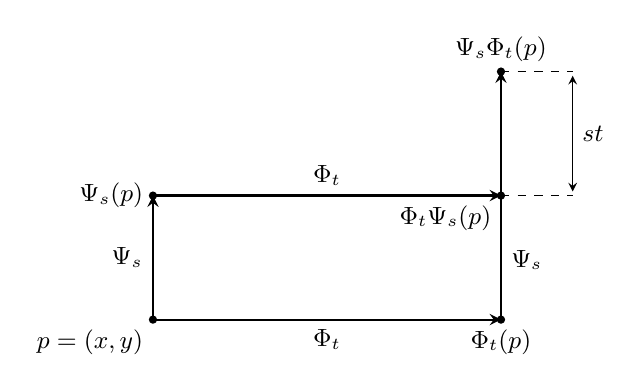
\begin{tikzpicture}[>=stealth,x=1.3cm,y=1.05cm,font=\small]
		\coordinate (P) at (0,0);
		\coordinate (XP) at (3.4,0);
		\coordinate (YP) at (0,1.5);
		\coordinate (XYP) at (3.4,1.5);
		\coordinate (YXP) at (3.4,3);
		\draw[->,thick] (P)--node[below] {\(\Phi_t\)} (XP);
		\draw[->,thick] (P)--node[left] {\(\Psi_s\)} (YP);
		\draw[->,thick] (YP)--node[above] {\(\Phi_t\)} (XYP);
		\draw[->,thick] (XP)--node[right,pos=.24] {\(\Psi_s\)} (YXP);
		\draw[dashed] (XYP)--(4.1,1.5);
		\draw[dashed] (YXP)--(4.1,3);
		\draw[<->] (4.1,1.55)--node[right] {\(st\)} (4.1,2.95);
		\foreach \Q in {P,XP,YP,XYP,YXP} \fill (\Q) circle (1.5pt);
		\node[below left] at (P) {\(p=(x,y)\)};
		\node[below] at (XP) {\(\Phi_t(p)\)};
		\node[left] at (YP) {\(\Psi_s(p)\)};
		\node[below left] at (XYP) {\(\Phi_t\Psi_s(p)\)};
		\node[above] at (YXP) {\(\Psi_s\Phi_t(p)\)};
	\end{tikzpicture}
	\caption{\(X=\partial_x\)、\(Y=x\partial_y\) 的两种运动次序，图中以 \(x,s,t>0\) 示意。先作水平运动会增加随后竖直运动的速度，两个终点的竖直差为 \(st\)。}
	\label{g1:fig:flow-order}
\end{figure}


\subsection{张量场的 Lie 导数}
\label{g1:subsec:1303:03}

流不仅可以搬运向量，也可以搬运度量、形式以及其他张量。\cref{g1:prop:mixed-tensor-pullback}已经说明，微分同胚拉回一个 \((r,s)\) 型张量时，对每个向量因子使用逆微分，对每个对偶因子使用微分的对偶。因此对 \(X\) 的流 \(\Phi\)，
\[
	\bigl((\Phi_t)^*T\bigr)_p
	=\left(\bigl(\mathrm{d}(\Phi_t)_p\bigr)^{-1}\right)^{\otimes r}
	\otimes\left(\bigl(\mathrm{d}(\Phi_t)_p\bigr)^*\right)^{\otimes s}
	\bigl(T_{\Phi_t(p)}\bigr).
\]
这个表达始终位于 \(T^r_s(\mathrm{T}_pM)\)，可以在固定纤维中对时间求导。

\begin{definition}
	\label{g1:def:lie-derivative-tensor}
	设 \(M\) 为无边界光滑流形，\(X\in\mathfrak X(M)\)，\(T\) 为光滑 \((r,s)\) 型张量场。定义 \(T\) 沿 \(X\) 的\term[lidaoshu]{Lie 导数}[Lie derivative]为
	\[
		\mathcal L_XT=\left.\frac{\mathrm{d}}{\mathrm{d}t}\right|_{t=0}(\Phi_t^X)^*T.
	\]
	导数在各点固定的张量纤维中取。局部流对时间和初值光滑，张量拉回的局部公式也光滑，因此这一定义给出同型的光滑张量场。
\end{definition}

在函数上有 \(\mathcal L_Xf=Xf\)，在向量场上有 \(\mathcal L_XY=[X,Y]\)。所以 Lie 导数扩展了同一个沿流比较的想法，无需另选内积或联络；它比较的方式由 \(X\) 的流本身确定。

\begin{proposition}[张量 Lie 导数的计算]
	\label{g1:prop:lie-derivative-tensor-rules}
	设 \(M\) 为无边界光滑流形，\(X\in\mathfrak X(M)\)，\(T,S\) 为光滑张量场，\(f\) 为光滑函数。Lie 导数实线性，并满足
	\[
		\mathcal L_X(T\otimes S)=(\mathcal L_XT)\otimes S+T\otimes(\mathcal L_XS),\qquad
		\mathcal L_X(fT)=X(f)T+f\mathcal L_XT.
	\]
	对任意指定位置的收缩 \(C\)，有 \(\mathcal L_X(CT)=C(\mathcal L_XT)\)。在局部坐标中，
	\begin{equation}
		\label{g1:eq:lie-derivative-tensor-coordinates}
		\begin{split}
			(\mathcal L_XT)^{i_1\cdots i_r}{}_{j_1\cdots j_s}
			={}&\sum_kX^k\partial_kT^{i_1\cdots i_r}{}_{j_1\cdots j_s}\\
			&-\sum_{a=1}^r\sum_k(\partial_kX^{i_a})
			T^{i_1\cdots i_{a-1}k i_{a+1}\cdots i_r}{}_{j_1\cdots j_s}\\
			&+\sum_{b=1}^s\sum_k(\partial_{j_b}X^k)
			T^{i_1\cdots i_r}{}_{j_1\cdots j_{b-1}k j_{b+1}\cdots j_s}.
		\end{split}
	\end{equation}
	此外，在流的共同定义域内，
	\[
		\frac{\mathrm{d}}{\mathrm{d}t}(\Phi_t^X)^*T
		=(\Phi_t^X)^*(\mathcal L_XT)
		=\mathcal L_X\bigl((\Phi_t^X)^*T\bigr).
	\]
	因此 \(\mathcal L_XT=0\) 当且仅当 \(T\) 被 \(X\) 的局部流保持。
\end{proposition}
\begin{proof}
	拉回保持张量积与收缩，见\cref{g1:prop:mixed-tensor-pullback}。对这些恒等式在 \(t=0\) 求导，用通常的乘积求导法则，便得到前两条乘法公式及收缩相容性。它也保持因子的排列，因此对称张量和交替张量的 Lie 导数仍保持各自的对称性。

	为得到坐标公式，先计算坐标基及对偶基的导数。向量场情形已知
	\[
		\mathcal L_X\partial_i=[X,\partial_i]=-\sum_k(\partial_iX^k)\partial_k.
	\]
	对任意一形式 \(\alpha\) 与向量场 \(Y\)，拉回和求值相容：
	\[
		(\Phi_t)^*(\alpha(Y))=((\Phi_t)^*\alpha)((\Phi_t)^*Y).
	\]
	在零时刻求导，得到
	\begin{equation}
		\label{g1:eq:lie-one-form-evaluation}
		(\mathcal L_X\alpha)(Y)=X(\alpha(Y))-\alpha([X,Y]).
	\end{equation}
	令 \(\alpha=\mathrm{d}x^j\)、\(Y=\partial_i\)，由于 \(\mathrm{d}x^j(\partial_i)=\delta_i^j\) 为常数，便有
	\[
		\mathcal L_X(\mathrm{d}x^j)=\sum_i(\partial_iX^j)\,\mathrm{d}x^i.
	\]
	将 \(T\) 在坐标张量基中展开，分别对系数、每个向量基因子及每个对偶基因子求导，就得到\eqref{g1:eq:lie-derivative-tensor-coordinates}。上指标的负号来自向量基的导数，下指标的正号来自对偶基的导数。

	最后，与\cref{g1:prop:flow-pullback-derivative}的证明一样，在一个共同定义的邻域中分别用
	\[
		(\Phi_{t+h})^*=(\Phi_t)^*(\Phi_h)^*
		=(\Phi_h)^*(\Phi_t)^*
	\]
	对 \(h\) 在零处求导，得到一般时间的两个等式。若 \(\mathcal L_XT=0\)，固定 \(p\) 后，\(\bigl((\Phi_t)^*T\bigr)_p\) 在固定有限维张量空间中导数为零，故等于 \(T_p\)；反向只需在 \(t=0\) 求导。
\end{proof}

同样对一般求值恒等式求导，可以得到一个无需坐标的计算方法。若 \(T\) 为协变 \(k\) 阶张量，则
\begin{equation}
	\label{g1:eq:lie-covariant-evaluation}
	(\mathcal L_XT)(Y_1,\ldots,Y_k)
	=X\bigl(T(Y_1,\ldots,Y_k)\bigr)
	-\sum_{a=1}^kT(Y_1,\ldots,[X,Y_a],\ldots,Y_k).
\end{equation}
右端第一项对整个实值函数求导，后面的各项扣除输入向量场随流变化的影响。对混合张量，还要对每个协变向量输入扣除对应的 \(\mathcal L_X\alpha\) 项；这由相同的求值乘积法则得到。只保留第一个方向导数而省略输入的修正，一般不会得到张量运算。

\begin{example}[膨胀下的张量变化]
	\label{g1:exm:lie-dilation-tensors}
	在 \(\mathbb R^n\) 上令 \(X=\sum_i x^i\partial_i\)，其流为 \(\Phi_t(x)=e^t x\)。常向量场和坐标一形式的拉回分别满足
	\[
		(\Phi_t)^*\partial_i=e^{-t}\partial_i,\qquad
		(\Phi_t)^*(\mathrm{d}x^i)=e^t\,\mathrm{d}x^i.
	\]
	所以 \(\mathcal L_X\partial_i=-\partial_i\)，而 \(\mathcal L_X(\mathrm{d}x^i)=\mathrm{d}x^i\)。Euclid 内积与标准最高次形式因而满足
	\[
		\mathcal L_X\left(\sum_i\mathrm{d}x^i\otimes\mathrm{d}x^i\right)
		=2\sum_i\mathrm{d}x^i\otimes\mathrm{d}x^i,\qquad
		\mathcal L_X(\mathrm{d}x^1\wedge\cdots\wedge\mathrm{d}x^n)
		=n\,\mathrm{d}x^1\wedge\cdots\wedge\mathrm{d}x^n.
	\]
	这些张量的坐标系数都是常数，Lie 导数却不为零，因为膨胀会改变向量输入的尺度。相反，对任意常数倍平移场，流的微分是恒等映射，这些常系数张量的 Lie 导数为零。
\end{example}

\subsection{自然性及分次 Cartan 运算的准备}
\label{g1:subsec:1303:04}

讨论映射与 Lie 括号的相容性时，不能沿任意光滑映射直接“推出一个向量场”。微分确实把单个切向量向前送，但同一目标点可能有多个原像，得到的向量未必一致；也可能目标方向根本不在微分的像中。需要明确要求两边的场彼此对应。

\begin{definition}
	\label{g1:def:related-vector-fields}
	设 \(F:M\to N\) 为无边界光滑流形之间的光滑映射。若 \(X\in\mathfrak X(M)\)、\(\overline X\in\mathfrak X(N)\) 满足
	\[
		\mathrm{d}F_pX_p=\overline X_{F(p)}\qquad(p\in M),
	\]
	称它们为 \(F\)-\term[xiangguanxiangliangchang]{相关向量场}[related vector fields]。
\end{definition}

由\cref{g1:def:manifold-differential}，相关条件等价于对目标上的每个局部光滑函数 \(f\) 有
\[
	X(f\circ F)=(\overline Xf)\circ F.
\]
反向也成立，因为将这一等式用于目标坐标函数，就能逐分量确定两个目标切向量相等。因此相关条件可以用函数检验，无需给 \(F\) 额外的可逆性。

\begin{proposition}[Lie 导数的自然性]
	\label{g1:prop:lie-derivative-natural}
	设 \(F:M\to N\) 为无边界光滑流形之间的光滑映射，\(X,\overline X\) 为 \(F\)-相关向量场。
	\begin{enumerate}
		\item 若 \(Y,\overline Y\) 也 \(F\)-相关，则 \([X,Y]\) 与 \([\overline X,\overline Y]\) \(F\)-相关。
		\item 记 \(X,\overline X\) 的局部流为 \(\Phi,\overline\Phi\)，则在每个初始点附近的充分小共同时间内，
		\[
			F\circ\Phi_t=\overline\Phi_t\circ F.
		\]
		\item 对 \(N\) 上任意光滑协变张量 \(T\)，有
		\[
			\mathcal L_X(F^*T)=F^*(\mathcal L_{\overline X}T).
		\]
		若 \(F\) 为局部微分同胚，同式也适用于任意混合张量。对任意微分形式 \(\alpha\)，无须可逆性即有
		\[
			\iota_X(F^*\alpha)=F^*(\iota_{\overline X}\alpha).
		\]
	\end{enumerate}
\end{proposition}
\begin{proof}
	对任意目标局部函数 \(f\)，连续使用相关条件可得
	\[
		\begin{aligned}
			[X,Y](f\circ F)
			&=X\bigl((\overline Yf)\circ F\bigr)
			-Y\bigl((\overline Xf)\circ F\bigr)\\
			&=(\overline X\overline Yf-\overline Y\overline Xf)\circ F
			=([\overline X,\overline Y]f)\circ F.
		\end{aligned}
	\]
	由函数检验条件得到第一项。这里既没有使用单射性，也没有使用满射性。

	对固定 \(p\)，曲线 \(t\mapsto F(\Phi_t(p))\) 的导数为
	\[
		\mathrm{d}F_{\Phi_t(p)}X_{\Phi_t(p)}
		=\overline X_{F(\Phi_t(p))},
	\]
	初值为 \(F(p)\)。它与 \(t\mapsto\overline\Phi_t(F(p))\) 满足同一初值问题，故在共同时间内相同。局部流的开定义域和连续性允许在 \(p\) 的一个邻域中同时选取充分小的时间区间，得到第二项的局部映射恒等式。

	协变张量的拉回始终有定义，并与复合相容，见\cref{g1:prop:covariant-tensor-pullback}。将第二项拉回，得到
	\[
		\Phi_t^*(F^*T)=F^*(\overline\Phi_t^*T).
	\]
	对 \(t\) 在零处求导，得到第三项的 Lie 导数公式。右边的 \(F^*\) 由固定的微分 \(\mathrm{d}F\) 作用于各输入，局部表达是固定系数与张量分量的有限次乘法和求和，所以求导可以穿过它。若 \(F\) 为局部微分同胚，各微分可逆，\cref{g1:prop:mixed-tensor-pullback}使同一个论证也适用于混合张量。

	最后，对任意 \(v_1,\ldots,v_{k-1}\in \mathrm{T}_pM\)，有
	\[
		\begin{aligned}
			\bigl(\iota_XF^*\alpha\bigr)_p(v_1,\ldots,v_{k-1})
			&=\alpha_{F(p)}(\mathrm{d}F_pX_p,\mathrm{d}F_pv_1,\ldots,\mathrm{d}F_pv_{k-1})\\
			&=\alpha_{F(p)}(\overline X_{F(p)},\mathrm{d}F_pv_1,\ldots,\mathrm{d}F_pv_{k-1}),
		\end{aligned}
	\]
	恰为右端的值。零次形式时两边均为零。
\end{proof}

若 \(F\) 是微分同胚，可以定义目标向量场
\[
	(F_*X)_q=\mathrm{d}F_{F^{-1}(q)}X_{F^{-1}(q)}.
\]
此时相关性自动成立，命题给出 \(F_*[X,Y]=[F_*X,F_*Y]\)。但对于投影 \(P(x,y)=x\)，向量场 \(y\partial_x\) 在不同原像 \((x,y)\) 上会送出不同的目标速度，因此没有与它相关的目标向量场。自然性命题的假设不能由“映射光滑”代替。

\ProseParagraphBreak

最后整理微分形式上的两个运算。\(\mathcal L_X\) 保持形式次数，\(\iota_X\) 将次数降低 \(1\)，并在函数上取零。\cref{g1:prop:interior-product-rule}已经证明
\[
	\iota_X(\alpha\wedge\beta)
	=(\iota_X\alpha)\wedge\beta+(-1)^p\alpha\wedge(\iota_X\beta),
	\qquad \alpha\in\Omega^p(M).
\]
符号来自将被插入的向量越过前面 \(p\) 个输入位置。把这类带次数的运算放在一起时，合适的交换子是
\[
	[A,B]_{\mathrm{gr}}=A\circ B-(-1)^{ab}B\circ A,
\]
其中 \(a,b\) 是各自改变形式次数的数。这称为分次交换子；两个次数为 \(-1\) 的运算之间对应的是反交换和，而不是普通差。

\begin{proposition}[插入与 Lie 导数]
	\label{g1:prop:cartan-insertion-identities}
	设 \(M\) 为无边界光滑流形，\(X,Y\in\mathfrak X(M)\)，\(\alpha,\beta\) 为微分形式。则
	\[
		\mathcal L_X(\alpha\wedge\beta)
		=(\mathcal L_X\alpha)\wedge\beta+\alpha\wedge(\mathcal L_X\beta),
	\]
	并且
	\begin{align*}
		\iota_X\iota_Y+\iota_Y\iota_X&=0,\\
		\mathcal L_X\iota_Y-\iota_Y\mathcal L_X&=\iota_{[X,Y]},\\
		\mathcal L_X\mathcal L_Y-\mathcal L_Y\mathcal L_X&=\mathcal L_{[X,Y]}.
	\end{align*}
	最后一式也适用于任意混合张量场。
\end{proposition}
\begin{proof}
	拉回保持楔积，故对 \(\Phi_t^*(\alpha\wedge\beta)=\Phi_t^*\alpha\wedge\Phi_t^*\beta\) 在零时刻求导，得到第一式。Lie 导数的次数是零，因此第二项前没有额外的分次符号。

	对至少二次的形式 \(\alpha\)，先插入 \(Y\)，再插入 \(X\)，得到
	\[
		(\iota_X\iota_Y\alpha)(v_1,\ldots)=\alpha(Y,X,v_1,\ldots).
	\]
	反向次序给出 \(\alpha(X,Y,v_1,\ldots)\)，由交替性二者相加为零。次数为零或一时，两次插入都给出零，因此第一条交换关系对所有次数成立。

	取 \(X\) 的局部流 \(\Phi\)。\cref{g1:prop:lie-derivative-natural}的插入相容性用于微分同胚 \(\Phi_t\)，其中源向量场是 \(\Phi_t^*Y\)，得到
	\[
		\Phi_t^*(\iota_Y\alpha)
		=\iota_{\Phi_t^*Y}(\Phi_t^*\alpha).
	\]
	插入对向量场和形式各自线性，且逐点为双线性运算。对右端用乘积求导法则，并用 \(\left.\partial_t\right|_0\Phi_t^*Y=[X,Y]\)，便得
	\[
		\mathcal L_X(\iota_Y\alpha)
		=\iota_{[X,Y]}\alpha+\iota_Y(\mathcal L_X\alpha),
	\]
	这就是第二条交换关系。

	为证明最后一条，记 \(D=\mathcal L_X\mathcal L_Y-\mathcal L_Y\mathcal L_X-\mathcal L_{[X,Y]}\)。两个次数为零的张量积导子的交换子仍是张量积导子：将它作用于 \(T\otimes S\)，展开后交叉项 \((\mathcal L_XT)\otimes(\mathcal L_YS)\) 与 \((\mathcal L_YT)\otimes(\mathcal L_XS)\) 分别抵消，余下的正是两端各自求导之和。因此 \(D\) 是张量积导子，并且与收缩相容。

	在函数上，\(Df=XYf-YXf-[X,Y]f=0\)。在向量场 \(Z\) 上，由 Jacobi 恒等式，
	\[
		DZ=[X,[Y,Z]]-[Y,[X,Z]]-[[X,Y],Z]=0.
	\]
	对任意一形式 \(\eta\) 与局部向量场 \(Z\)，求值是张量积之后的收缩，所以
	\[
		0=D(\eta(Z))=(D\eta)(Z)+\eta(DZ)=(D\eta)(Z).
	\]
	取坐标向量场逐个检验，得到 \(D\eta=0\)。任意张量在局部都是光滑函数乘若干向量场与一形式的张量积之和，导子法则遂给出 \(DT=0\)。这证明了所有混合张量上的最后一式，形式情形包含在其中。
\end{proof}

这些等式把运动、插入和交替性联系起来。在\secref{g1:sec:1401}中，将构造把形式次数提高 \(1\) 的外微分 \(\mathrm{d}\)，并证明 Cartan 公式\footnote{Cartan，Élie Joseph Cartan（1869--1951），法国数学家，研究 Lie 群、Lie 代数与微分几何，发展了活动标架方法。}
\[
	\mathcal L_X=\mathrm{d}\iota_X+\iota_X\mathrm{d}.
\]
这里的加号与两个奇次数运算的分次交换子相符；定义外微分以后，将给出该公式及其证明。
% 纲要条目排为编号小节标题，并进入目录与书签；说明段仍保留于纲要注释中。

% !TeX root = ../../Book1.tex
% 纲要标题：### 13.4 Frobenius 定理与积分叶
% 纲要位置：几何学计划纲要.md，第 627 行。
% 正文状态：初稿；尚未正式审核。

% 纲要内容开始
% 
% * 分布、局部标架与积分流形
% * 对合条件的必要性
% * 对合分布的交换化标架
% * 适应坐标和局部积分叶的构造
% * 最大连通积分叶及唯一性
% 
% 纲要内容结束

\section{Frobenius 定理与积分叶}
\label{g1:sec:1304}

给定一条非零向量场，可以沿其积分曲线组织局部坐标。如果在每一点指定的是一个 \(r\) 维切平面，能否找到 \(r\) 维子流形，使它在各点的切空间恰好等于所指定的平面？这里的困难不只是分别沿 \(r\) 个方向求积分曲线：先沿一个方向、再沿另一个方向移动，可能产生离开原平面的额外方向。Lie 括号正好测量这种不相容性。

\ProseParagraphBreak

本节始终在有限维、Hausdorff、第二可数且无边界的光滑流形上讨论常秩光滑分布。证明先把对合分布的局部标架换成两两交换的标架，再用交换流构造坐标。局部坐标片的粘合会给出最大连通积分叶；叶片的粘合还将赋予叶自身的拓扑，并保证 Hausdorff 性和第二可数性。

\subsection{分布、局部标架与积分流形}
\label{g1:subsec:1304:01}

\begin{definition}[光滑分布]\label{g1:def:smooth-distribution}
	设 \(M^n\) 为无边界光滑流形，\(0\le r\le n\)。切丛 \(\mathrm{T}M\) 的秩 \(r\) 光滑向量子丛 \(D\subseteq \mathrm{T}M\) 称为一个秩 \(r\) 的\term[guanghuafenbu]{光滑分布}[smooth distribution]。等价地，在每个 \(p\in M\) 的某邻域 \(U\) 上，存在光滑向量场 \(Z_1,\ldots,Z_r\)，使它们在每一点线性无关，且
	\[
		D_q=\operatorname{span}\{Z_1(q),\ldots,Z_r(q)\}\qquad(q\in U).
	\]
	这样的向量场组称为 \(D\) 的局部标架。记 \(\Gamma(U,D)\) 为 \(U\) 上所有取值于 \(D\) 的光滑向量场。
\end{definition}

这个等价描述正是\cref{g1:def:vector-subbundle}对 \(\mathrm{T}M\) 的应用。固定维数还不够，局部标架的光滑性也属于条件。另一方面，“取值于 \(D\) 的光滑向量场”确实是子丛的光滑截面：由\cref{g1:prop:subbundle-adapted-frame}把局部标架补成 \(\mathrm{T}M\) 的标架后，后面的分量恒为零，前面的分量仍光滑。因而任意 \(X\in\Gamma(U,D)\) 都唯一写为
\[
	X=\sum_{i=1}^r f^iZ_i
\]
且各 \(f^i\) 光滑。

\begin{definition}[积分流形]\label{g1:def:integral-manifold}
	设 \(D\subseteq \mathrm{T}M\) 为秩 \(r\) 光滑分布。一个 \(r\) 维无边界光滑流形 \(N\)，连同单射浸入 \(\iota:N\to M\)，若满足
	\[
		\mathrm{d}\iota_q(\mathrm{T}_qN)=D_{\iota(q)}\qquad(q\in N),
	\]
	则称为 \(D\) 的一个\term[jifenliuxing]{积分流形}[integral manifold]。把 \(N\) 与其像识别时，像使用从 \(N\) 搬来的流形拓扑和光滑结构，不预先要求它们等于子空间拓扑及嵌入子流形结构。若每个 \(p\in M\) 都位于某个积分流形的像内，则称 \(D\) 可积。
\end{definition}

这里单射使一个像点只有一个参数点，浸入则保证局部参数确实给出一块 \(r\) 维曲面。然而，\cref{g1:exm:injective-immersion-not-embedding}已经说明，单射浸入未必是嵌入：可能有环境空间中相近的点，在参数流形中相距很远。因此积分流形的拓扑可以比像的子空间拓扑更细。后面构造最大叶时，会明确选出这个拓扑。

\begin{example}\label{g1:exm:submersion-integral-levels}
	若 \(F:M^n\to N^{n-r}\) 是光滑淹没，则 \(D=\ker\mathrm{d}F\) 为秩 \(r\) 光滑分布。其子丛性质来自\cref{g1:thm:constant-rank-bundle-morphism}：把 \(\mathrm{d}F\) 看成 \(\mathrm{T}M\to F^*\mathrm{T}N\) 的满射丛同态，其核秩恒为 \(r\)。对每个非空水平集 \(F^{-1}(y)\)，\cref{g1:thm:regular-level-set}给出嵌入子流形结构，且
	\[
		\mathrm{T}_pF^{-1}(y)=\ker\mathrm{d}F_p=D_p.
	\]
	因此水平集及其连通分支都是积分流形。在这个例子中，积分流形由一些保持不变的函数值刻画；\term[frobeniusdingli]{Frobenius 定理}[Frobenius theorem]\footnote{Frobenius，Ferdinand Georg Frobenius（1849--1917），德国数学家，研究群的表示与特征标以及微分方程。}将证明，对合条件正好保证局部总能找到这样的横向坐标函数。
\end{example}

秩零分布的连通积分流形是单点；秩 \(n\) 的分布只能是 \(\mathrm{T}M\)，其局部积分流形是开集。以下证明也包含这两个情形，空的标架或横向坐标按通常的零维约定理解。

\subsection{对合条件的必要性}
\label{g1:subsec:1304:02}

若两条向量场都沿同一个积分流形运动，它们的无穷小交换也应当沿这个流形。为把这个直观判断写成坐标无关的条件，我们使用\cref{g1:def:lie-bracket}中的括号
\[
	[X,Y]f=X(Yf)-Y(Xf).
\]

\begin{definition}[对合分布]\label{g1:def:involutive-distribution}
	设 \(D\subseteq \mathrm{T}M\) 为光滑分布。若对任意开集 \(U\subseteq M\) 及任意 \(X,Y\in\Gamma(U,D)\)，都有
	\[
		[X,Y]\in\Gamma(U,D),
	\]
	则称 \(D\) 为\term[duihefenbu]{对合分布}[involutive distribution]。
\end{definition}

检查对合性时，只需检查一组局部标架的两两括号。事实上，由\cref{g1:prop:lie-bracket-properties}的乘积法则，
\[
	\left[\sum_i f^iZ_i,\sum_j g^jZ_j\right]
	=\sum_{i,j}f^ig^j[Z_i,Z_j]
	+\sum_{i,j}f^iZ_i(g^j)Z_j
	-\sum_{i,j}g^jZ_j(f^i)Z_i.
\]
后两项自动取值于 \(D\)，第一项则由标架括号条件控制。对合不要求原标架彼此交换。例如 \(\mathrm{T}\mathbb R^2\) 的标架 \(\partial_x,e^x\partial_y\) 满足 \([\partial_x,e^x\partial_y]=e^x\partial_y\ne0\)，但括号仍在该分布中。秩一分布自动对合，因为 \([fX,gX]=(fXg-gXf)X\)。

\begin{proposition}[可积性的必要条件]\label{g1:prop:involutivity-necessary}
	设 \(M\) 为无边界光滑流形，\(D\subseteq \mathrm{T}M\) 为常秩光滑分布。若每个点都有通过它的积分流形，则 \(D\) 对合。更具体地，若 \(\iota:N\to M\) 是一个积分流形，\(X,Y\) 为某开集 \(U\) 上取值于 \(D\) 的光滑向量场，则 \([X,Y]\) 在 \(U\cap\iota(N)\) 上也取值于 \(D\)。
\end{proposition}
\begin{proof}
	在 \(\iota^{-1}(U)\) 上，因 \(\mathrm{d}\iota_q:\mathrm{T}_qN\to D_{\iota(q)}\) 为线性同构，可唯一定义向量场 \(\widetilde X,\widetilde Y\)，使
	\[
		\mathrm{d}\iota\,\widetilde X=X\circ\iota,\qquad
		\mathrm{d}\iota\,\widetilde Y=Y\circ\iota.
	\]
	它们光滑。具体地，在局部标架中，\(\mathrm{d}\iota\) 给出到拉回分布 \(\iota^*D\) 的光滑可逆矩阵；其逆由伴随矩阵除以非零行列式给出，故光滑，正如\cref{g1:prop:bundle-morphism-matrices}所述。

	相关向量场的括号仍相关，见\cref{g1:prop:lie-derivative-natural}。当前所用的计算很短：对 \(f\in C^\infty(U)\)，有
	\[
		\begin{aligned}
			[\widetilde X,\widetilde Y](f\circ\iota)
			&=\widetilde X\bigl((Yf)\circ\iota\bigr)-\widetilde Y\bigl((Xf)\circ\iota\bigr)\\
			&=([X,Y]f)\circ\iota.
		\end{aligned}
	\]
	以导子判断切向量，得到
	\[
		[X,Y]_{\iota(q)}
		=\mathrm{d}\iota_q\bigl([\widetilde X,\widetilde Y]_q\bigr)
		\in \mathrm{d}\iota_q(\mathrm{T}_qN)=D_{\iota(q)}.
	\]
	若每个点都有这样的积分流形，就在每一点得到所需的包含关系，故 \([X,Y]\) 为 \(D\) 的光滑截面。
\end{proof}

浸入微分把 \(\mathrm{T}N\) 同构到沿像的 \(D\)，因而能将局部的分布截面提升到积分流形；括号自然性随后把它们的括号送回 \(D\)。

\subsection{对合分布的交换化标架}
\label{g1:subsec:1304:03}

对合条件只说 \([Z_i,Z_j]\) 能用原标架线性表示，而交换流需要的是括号等于零。关键在于先选择若干坐标方向，使它们在 \(D\) 上能够独立测量所有分量，再把这些分量归一化。这样新标架的括号既必须留在 \(D\)，又失去了在这些方向上的全部分量，只能为零。

\begin{lemma}[交换化分布标架]\label{g1:lem:commuting-distribution-frame}
	设 \(D\) 为无边界光滑流形 \(M^n\) 上的秩 \(r\) 对合光滑分布。对每个 \(p\in M\)，存在以 \(p\) 为原点的坐标
	\[
		(x^1,\ldots,x^r,y^1,\ldots,y^{n-r})
	\]
	及 \(D\) 的光滑局部标架 \(X_1,\ldots,X_r\)，满足
	\begin{equation}\label{g1:eq:normalized-distribution-frame}
		X_i=\frac{\partial}{\partial x^i}
		+\sum_{\alpha=1}^{n-r}a_i^\alpha(x,y)\frac{\partial}{\partial y^\alpha},
		\qquad [X_i,X_j]=0.
	\end{equation}
\end{lemma}
\begin{proof}
	先取任意局部标架 \(Z_1,\ldots,Z_r\) 和环境坐标 \(z^1,\ldots,z^n\)。在 \(p\) 处，系数矩阵 \((Z_jz^a)_{a,j}\) 的秩为 \(r\)，所以有一个非零的 \(r\) 阶子式。重排坐标后，可令它由前 \(r\) 行给出，记这部分坐标为 \(x\)，其余为 \(y\)。缩小邻域使
	\[
		B_{aj}=Z_jx^a\qquad(1\le a,j\le r)
	\]
	始终可逆，并定义
	\[
		X_i=\sum_{j=1}^r(B^{-1})_{ji}Z_j.
	\]
	逆矩阵光滑，新向量场仍为 \(D\) 的标架；并且
	\[
		X_ix^a=\sum_jB_{aj}(B^{-1})_{ji}=\delta_i^a.
	\]
	这就给出\eqref{g1:eq:normalized-distribution-frame}中的第一式。

	投影到前 \(r\) 个坐标的微分 \(\mathrm{d}x:D_q\to\mathbb R^r\) 在整个邻域中为同构，因为它把 \(X_i(q)\) 送到第 \(i\) 个标准基向量。另一方面，
	\[
		[X_i,X_j]x^a=X_i(\delta_j^a)-X_j(\delta_i^a)=0.
	\]
	所以括号的全部 \(x\) 分量为零。同时，对合性使它属于 \(D_q\)。一个属于 \(D_q\) 且被 \(\mathrm{d}x\) 送到零的向量只能为零，故 \([X_i,X_j]=0\)。
\end{proof}

这一步只换了分布的标架，还没有找到使 \(X_i\) 本身成为坐标向量的坐标。后一任务由流完成。若直接展开刚才消失的横向分量，还可把对合条件写为
\[
	\partial_{x^i}a_j^\alpha-\partial_{x^j}a_i^\alpha
	+\sum_{\beta=1}^{n-r}\left(
		a_i^\beta\partial_{y^\beta}a_j^\alpha
		-a_j^\beta\partial_{y^\beta}a_i^\alpha
	\right)=0.
\]
这些是系数之间的相容方程；不必另外求解这组偏微分方程，交换的局部流会直接给出积分片。

\subsection{适应坐标和局部积分叶的构造}
\label{g1:subsec:1304:04}

交换化标架给出沿各个允许方向的交换流。把这些流依次作用在一张横向小截面上，流时间与截面坐标便组成候选坐标；逆函数定理将证明它们确实覆盖一个邻域。

\begin{theorem}[Frobenius 定理]\label{g1:thm:frobenius}
	设 \(M^n\) 为有限维、Hausdorff、第二可数且无边界的光滑流形，\(D\subseteq \mathrm{T}M\) 为秩 \(r\) 光滑分布。下列条件等价：
	\begin{enumerate}
		\item \(D\) 对合；
		\item 每个点附近都有坐标 \((u^1,\ldots,u^r,v^1,\ldots,v^{n-r})\)，使
		\[
			D=\operatorname{span}\left\{\frac{\partial}{\partial u^1},\ldots,\frac{\partial}{\partial u^r}\right\};
		\]
		\item 每个点都位于某个 \(r\) 维积分流形内。
	\end{enumerate}
	第二项中的坐标域可取为乘积 \(B\times T\)，其中 \(B\subseteq\mathbb R^r\)、\(T\subseteq\mathbb R^{n-r}\) 为开球或开盒；固定 \(v=c\) 的切片给出局部嵌入积分流形。
\end{theorem}
\begin{proof}
	设 \(D\) 对合。固定 \(p\)，用\cref{g1:lem:commuting-distribution-frame}取得局部坐标 \((x,y)\) 和两两交换的标架 \(X_1,\ldots,X_r\)。令 \(\Phi_i^t\) 为 \(X_i\) 的局部流。\cref{g1:thm:maximal-local-flow,g1:thm:ode-smooth-dependence}保证它们在零时间附近存在，且对时间与初值联合光滑；不需要这些向量场完备。由\cref{g1:thm:commuting-local-flows}，在足够小的共同邻域内，各局部流两两交换。

	取横截片 \(\sigma(y)=(0,y)\)，定义
	\begin{equation}\label{g1:eq:frobenius-flow-coordinates}
		\Psi(t,y)=\Phi_r^{t^r}\circ\cdots\circ\Phi_1^{t^1}(\sigma(y)).
	\end{equation}
	这时必须使一个参数盒内的全部复合都有定义。因为只有有限条流及交换时所需的有限种复合，零参数时所有中间点都在 \(p\) 附近；各流的定义域开放，故可同时缩小时间盒和横截片，使这些复合及其中间点都留在上述共同邻域。于是 \(\Psi\) 是一个开参数盒上的光滑映射。

	利用交换性，把第 \(i\) 条流移到最外层，便有
	\[
		\Psi(t+s e_i,y)=\Phi_i^s(\Psi(t,y))
	\]
	对充分小的 \(s\) 成立。在 \(s=0\) 求导得到
	\begin{equation}\label{g1:eq:frobenius-pushed-coordinate-fields}
		\mathrm{d}\Psi_{(t,y)}\!\left(\frac{\partial}{\partial t^i}\right)
		=X_i(\Psi(t,y)).
	\end{equation}
	在 \((0,0)\) 处，时间方向的导数为 \(X_i(p)\)，横截方向的导数为原坐标的 \(\partial_{y^\alpha}|_p\)。因此按 \((x,y)\) 排列的导数矩阵为
	\[
		\mathrm{D}\Psi(0,0)=
		\begin{pmatrix}
			I_r&0\\
			A&I_{n-r}
		\end{pmatrix},
		\qquad A_{\alpha i}=a_i^\alpha(p),
	\]
	它可逆。\cref{g1:thm:inverse-function}给出 \(\Psi\) 在原点附近的光滑逆；再把参数域缩小为乘积 \(B\times T\)，其像仍为开集 \(U\)，且 \(\Psi:B\times T\to U\) 为微分同胚。

	取 \((u,v)=\Psi^{-1}\) 为 \(U\) 上的新坐标。\eqref{g1:eq:frobenius-pushed-coordinate-fields}说明原来的 \(X_i\) 正好成为新坐标向量 \(\partial_{u^i}\)，从而得到第二项。秩零时没有流，直接使用原坐标；满秩时横截片是单点，同一个可逆矩阵论证仍成立。

	第二项推出第三项：固定 \(v=c\)，映射 \(u\mapsto\Psi(u,c)\) 是一块嵌入参数片，其微分像正是 \(D\)，故为积分流形。第三项推出第一项已经由\cref{g1:prop:involutivity-necessary}证明。
\end{proof}

在这样的适应坐标中，把 \(U\) 称为一个\term[yezhuangzuobiaohe]{叶状坐标盒}[foliation box]；对 \(c\in T\)，把
\[
	P_c=\Psi(B\times\{c\})
\]
称为该盒的一张\term[yepian]{叶片}[plaque]。叶片是连通的局部嵌入积分流形。这里的“叶片”只指一个盒中的局部切片，后面所说的“叶”则是最大连通积分流形，不宜混用。\cref{g1:fig:frobenius-plaques}中，横向坐标 \(v\) 区分不同叶片，沿 \(D\) 的运动只改变 \(u\)。

% !TeX root = ../Book1.tex
% 一维叶片的二维示意；一般情形由r维切片替代曲线。
\begin{figure}[htbp]
	\centering
	\begin{tikzpicture}[font=\small]
		\begin{scope}
			\node at (1.8,3.45) {参数盒 \(B\times T\)};
			\fill[GeometryBlueLight] (0,0) rectangle (3.6,3);
			\draw[GeometryGray,dashed] (0,0) rectangle (3.6,3);
			\draw[orange!75!black,thick] (1.8,0.25)--(1.8,2.75);
			\foreach \h in {0.65,2.35}{
				\draw[GeometryGray] (0.25,\h)--(3.35,\h);
			}
			\draw[GeometryBlue,very thick,->] (0.25,1.5)--(3.35,1.5);
			\fill[GeometryBlue] (1.8,1.5) circle[radius=2pt];
			\node[above,fill=GeometryBlueLight,inner sep=1.5pt] at (2.75,1.5) {\(v=c\)};
			\node[orange!75!black,above] at (1.8,2.8) {\(u=0\)};
			\draw[->,GeometryGray] (0.25,-0.35)--(3.35,-0.35) node[right] {\(u\)};
			\draw[->,GeometryGray] (-0.35,0.25)--(-0.35,2.8) node[above] {\(v\)};
		\end{scope}
		\draw[->,thick] (4.05,1.5)--(5.35,1.5) node[midway,above] {\(\Psi\)};
		\begin{scope}[xshift=5.8cm]
			\node at (1.8,3.45) {流形中的坐标邻域 \(U\)};
			\fill[GeometryBlueLight] (0,0) rectangle (3.6,3);
			\draw[GeometryGray,dashed] (0,0) rectangle (3.6,3);
			\draw[orange!75!black,thick] (1.8,0.25)--(1.8,2.75);
			\foreach \h in {0.65,2.35}{
				\draw[GeometryGray] (0.25,\h) .. controls (1.1,{\h+0.45}) and (2.5,{\h-0.45}) .. (3.35,\h);
			}
			\draw[GeometryBlue,very thick] (0.25,1.5) .. controls (1.1,1.95) and (2.5,1.05) .. (3.35,1.5);
			\draw[GeometryBlue,thick,->] (2.05,1.44)--(2.7,1.37);
			\fill[GeometryBlue] (1.8,1.5) circle[radius=2pt];
			\node[GeometryBlue,above] at (2.55,1.47) {\(D\)};
			\node[GeometryBlue,right] at (3.4,1.5) {\(P_c\)};
			\node[orange!75!black,above] at (1.8,2.8) {\(\sigma(y)\)};
		\end{scope}
	\end{tikzpicture}
	\caption{一维叶片的二维示意。固定横向坐标的切片经 \(\Psi\) 变成积分叶片 \(P_c\)，橙色线表示横截片，蓝色箭头表示分布方向。高秩情形用 \(r\) 维片替代曲线，横向坐标仍沿片保持不变。}
	\label{g1:fig:frobenius-plaques}
\end{figure}


\begin{lemma}[局部积分叶片的唯一性]\label{g1:lem:local-integral-plaque}
	设 \(M\) 为无边界光滑流形，\(D\) 为其上的秩 \(r\) 光滑分布。设开集 \(U\subset M\) 具有乘积坐标 \((u,v)\in B\times T\)，其中 \(B,T\) 为开球，且 \(D|_U=\operatorname{span}\{\partial_{u^1},\ldots,\partial_{u^r}\}\)。对 \(c\in T\)，以 \(P_c\) 记切片 \(\{(u,c):u\in B\}\) 在 \(U\) 中的原像。若 \(\iota:N\to M\) 是连通积分流形且 \(\iota(N)\subseteq U\)，则 \(v\circ\iota\) 为常值 \(c\)，且
	\[
		\iota:N\longrightarrow P_c
	\]
	是到 \(P_c\) 某开子集的微分同胚。因此，任何两个通过同一点的积分流形，在分别缩小其参数邻域后，像在该点附近一致。
\end{lemma}
\begin{proof}
	由于 \(\mathrm{d}\iota(\mathrm{T}N)=D\)，而每个横向坐标 \(v^\alpha\) 的微分在 \(D\) 上为零，故
	\[
		\mathrm{d}(v^\alpha\circ\iota)=0.
	\]
	光滑函数微分为零时局部常值：在源坐标小球内沿线段使用一元微积分，函数值不变。连通空间上的局部常值函数为常值，因为一个取值的原像及其补集都是开集。因此 \(v\circ\iota=c\)。

	前 \(r\) 个坐标的微分在 \(D\) 上为同构，所以
	\[
		\mathrm{d}(u\circ\iota)_q
		=\mathrm{d}u_{\iota(q)}\circ\mathrm{d}\iota_q:\mathrm{T}_qN\to\mathbb R^r
	\]
	可逆。逆函数定理表明 \(\iota:N\to P_c\) 是局部微分同胚，因此为开映射。它又单射，故是到其像的同胚，局部光滑逆粘合成整体光滑逆，像在 \(P_c\) 中开。

	最后，对两条通过同一点 \(p\) 的积分流形，先各取连通参数邻域，使像落在同一个适应坐标盒中。两者的横向常值都等于 \(v(p)\)，像都是同一 \(P_{v(p)}\) 中含 \(p\) 的开集。取这两个开集的交，再限制各参数邻域，即得到相同的局部像。
\end{proof}

若一条积分流形没有整个落在 \(U\) 内，只能把引理用于其原像 \(\iota^{-1}(U)\) 的各个连通分支。不同分支可以落在同一个坐标盒的不同叶片上。局部唯一性因此不表示一个完整的积分叶与 \(U\) 只能相交一张叶片，也不保证完整积分叶是嵌入的。

\subsection{最大连通积分叶及唯一性}
\label{g1:subsec:1304:05}

沿相交的叶片继续前进，可以把经过一点的所有局部积分片连在一起。首先需要确定哪些点属于同一片最大对象，然后给这个点集一个使各叶片成为开坐标片的拓扑。这个拓扑下，远行后重新靠近原点的部分不必成为原来那一张局部坐标片中的邻近点。

\begin{theorem}[最大连通积分叶]\label{g1:thm:maximal-connected-leaf}
	设 \(M\) 为有限维、Hausdorff、第二可数且无边界的光滑流形，\(D\subseteq \mathrm{T}M\) 为秩 \(r\) 对合光滑分布。对每个 \(p\in M\)，存在唯一的最大连通积分流形 \(L_p\)，其像包含 \(p\)。更精确地，\(L_p\) 是 \(M\) 的一个子集，带有 Hausdorff、第二可数的 \(r\) 维光滑流形结构，包含映射 \(i_p:L_p\hookrightarrow M\) 为浸入，且任何像包含 \(p\) 的连通积分流形 \(\iota:N\to M\) 都唯一分解为
	\[
		N\xrightarrow{\ \widehat\iota\ }L_p\xrightarrow{\ i_p\ }M,
	\]
	其中 \(\widehat\iota\) 是开嵌入。不同的 \(L_p\) 要么相同，要么不交，故它们将 \(M\) 分割成最大连通积分流形。这些最大积分流形称为 \(D\) 的\term[ye]{叶}[leaf]。
\end{theorem}
\begin{proof}
	先取至多可数个叶状坐标盒 \(U_1,U_2,\ldots\) 覆盖 \(M\)。第二可数性保证可以这样取：在一个可数拓扑基中，对每个能包含于某个给定坐标盒的基元素选一个这样的盒；每点附近都有这样的基元素，所以选出的至多可数个盒仍覆盖 \(M\)。记第 \(j\) 个盒的坐标为 \((u_j,v_j)\in B_j\times T_j\)，其叶片记为 \(P_{j,c}\)。

	如果存在有限叶片链
	\[
		P_0,P_1,\ldots,P_k,\qquad
		P_{\ell-1}\cap P_\ell\ne\varnothing,
	\]
	使两点分别位于首尾叶片，就称这两点可由叶片相连。每点属于某叶片，反转链给出对称性，拼接链给出传递性，所以这是等价关系。令 \(L_p\) 为 \(p\) 的等价类。若一个叶片与 \(L_p\) 相交，便可加到相应的有限链末尾，故整个叶片都包含于 \(L_p\)。

	先说明相交叶片的拓扑如何衔接。设 \(P,Q\) 为所选坐标盒中的两张叶片，且 \(z\in P\cap Q\)。在 \(P\) 内取 \(P\cap U_Q\) 中含 \(z\) 的一个小连通开邻域，其中 \(U_Q\) 是含 \(Q\) 的坐标盒。这个邻域是积分流形，像落在 \(U_Q\) 中，由\cref{g1:lem:local-integral-plaque}，它位于通过 \(z\) 的唯一叶片 \(Q\) 内。因此 \(P\cap Q\) 在 \(P\) 中开；交换二者，同样在 \(Q\) 中开。两张叶片坐标之间的转换，是环境坐标转换限制到这些开集后取前 \(r\) 个分量，因而光滑，其逆也光滑。

	给 \(L_p\) 如下拓扑：\(W\subseteq L_p\) 开，当且仅当对每张包含于 \(L_p\) 的上述叶片 \(P\)，交集 \(W\cap P\) 在 \(P\) 中开。刚才的交集性质说明每张 \(P\) 在这个拓扑中开，而且它的诱导拓扑恰好是原来的 Euclid 片拓扑。例如 \(P\) 中任一开集 \(V\) 与其他叶片 \(Q\) 的交，在开集 \(P\cap Q\) 内经光滑坐标转换仍为开集，因此 \(V\) 也是 \(L_p\) 的开集。各叶片坐标遂组成光滑相容图册。包含映射在每个片上就是坐标切片的包含，所以连续、光滑且微分像为 \(D\)。任意两点可在 \(M\) 中用不交开邻域分开，取这些邻域与 \(L_p\) 的交，仍为叶拓扑中的开集，故 \(L_p\) Hausdorff。

	接着验证第二可数性。这不能由“\(L_p\) 是第二可数空间 \(M\) 的子集”推出，因为刚定义的叶拓扑可能比子空间拓扑更细。我们证明这条叶实际只用到可数张叶片。固定一张叶片 \(P\) 以及一个坐标盒 \(U_j\)。集合 \(P\cap U_j\) 是 \(P\) 的开子集，至多有可数个连通分支：在 \(P\) 的 Euclid 坐标中，每个连通分支都是开集，因为每点的小球连通；不同非空分支各含一个不同的有理坐标点，故只有可数个。秩零时开子集至多为单点，结论同样成立。每个分支 \(C\) 是连通积分流形且位于 \(U_j\) 内，由局部唯一性，\(v_j|_C\) 常值，故 \(C\) 只遇到 \(U_j\) 中的一张叶片。因此对固定的 \(P,U_j\)，与 \(P\) 相交的 \(U_j\) 叶片至多可数。

	坐标盒本来只有可数个，故与固定 \(P\) 相交的全部所选叶片至多可数。现在从一张含 \(p\) 的叶片开始：第一步加入所有与它相交的叶片，第二步加入所有与第一步叶片相交的叶片，依此继续。每一步得到可数集合，可数步之并仍可数，并且恰好包含所有能用有限链从 \(p\) 到达的叶片。它们覆盖 \(L_p\)。每张叶片取一个可数 Euclid 拓扑基，所有这些基的并给出 \(L_p\) 的可数基，因为叶片是开坐标片。至此，\(L_p\) 确实是通常意义下的 Hausdorff、第二可数光滑流形。

	每张叶片同胚于开球或开盒，所以可以在片内用光滑路径连接两点。沿任一有限叶片链选择相邻交点并连接这些路径，得到叶内的连续分片光滑路径。因此 \(L_p\) 路径连通，尤其连通。

	最后证明最大性与唯一性。设 \(\iota:N\to M\) 为连通积分流形，且像包含 \(p\)。对任意 \(q\in N\)，选一个连通参数邻域，其像落在某个 \(U_j\) 内。局部唯一性说明这个像落在一张叶片中，所以 \(N\) 中映入同一叶片等价类的点构成开集；这些开集两两不交并覆盖 \(N\)。由连通性只有一个非空类，且它是 \(L_p\)。故 \(\iota\) 在集合意义下唯一地分解为 \(\widehat\iota:N\to L_p\)。

	在刚才的每个小参数邻域内，\(\widehat\iota\) 的像位于一张开叶片中，而\cref{g1:lem:local-integral-plaque}使它成为到该叶片开子集的微分同胚。因此 \(\widehat\iota\) 是局部微分同胚，特别地连续且开。它由 \(\iota\) 的单射性而单射，故为开嵌入。这证明 \(L_p\) 包含经过 \(p\) 的每个连通积分流形的像。任何另一个最大连通积分流形必须具有相同的像，两个结构之间的恒等映射又由上述分解在两个方向光滑，所以最大对象连同流形结构都唯一。最后，等价类本来相同或不交，故叶构成 \(M\) 的分割。
\end{proof}

这个由最大叶组成的分割，连同上述局部乘积坐标，称为 \(M\) 上的一个 \(r\) 维\term[yezhuangjiegou]{光滑叶状结构}[smooth foliation]，常记为 \(\mathcal F\)。各叶在每个坐标盒中分解为若干叶片；叶片之间的切向空间相容，合起来正是原来的分布 \(D\)。

\ProseParagraphBreak

这个证明同时给出了叶状坐标盒的内在用途：它们既提供叶的局部图，又用可数传播控制叶的整体拓扑。对任一固定盒，一条叶可能经过可数多张不同叶片，而不是只有一张；叶中的邻近由单张叶片上的坐标决定，环境中的再次靠近则未必意味着叶内的靠近。

\ProseParagraphBreak

Frobenius 定理由常秩、光滑性与对合条件得到局部适应坐标，并得到具有自身流形结构的最大连通叶。叶是否嵌入、压缩各叶所得商空间是否 Hausdorff，则取决于叶离开局部坐标盒后的整体行为。下一节将在环面流和横截面返回的模型中计算这些行为。

% 纲要条目排为编号小节标题，并进入目录与书签；说明段仍保留于纲要注释中。

% !TeX root = ../../Book1.tex
% 纲要标题：### 13.5 叶状结构的整体问题与不可积模型
% 纲要位置：几何学计划纲要.md，第 635 行。
% 正文状态：初稿；尚未正式审核。

% 纲要内容开始
% 
% * 环面上的有理和无理斜率叶
% * 横截面、返回映射及沿叶映射芽
% * 非 Hausdorff 叶空间
% * 标准接触分布的不可积性
% 
% ---
% 
% 纲要内容结束

\section{叶状结构的整体问题与不可积模型}
\label{g1:sec:1305}

Frobenius 定理给每个点附近一叠坐标切片，最大叶定理则说明怎样沿这些切片继续前进。继续以后会发生什么，仍须另外研究：一条叶可能闭合，也可能反复进入同一个坐标盒，甚至在整个流形中稠密；沿叶绕一圈后，邻近叶的横向位置也可能改变。本节用几个能够直接计算的模型分辨这些现象。全节的流形均无边界，分布均为常秩光滑分布。

\subsection{环面上的有理和无理斜率叶}
\label{g1:subsec:1305:01}

把二维环面写为 \(T^2=\mathbb R^2/\mathbb Z^2\)，即分别把两个坐标模 \(1\) 识别。局部坐标来自小矩形的商像，换坐标只是整数平移，所以常向量场
\[
	X_\alpha=\partial_x+\alpha\partial_y,\qquad \alpha\in\mathbb R,
\]
下降为环面上的处处非零光滑向量场。它的流为
\[
	\Phi_t([x,y])=[x+t,y+\alpha t].
\]
这给出一个处处秩一的分布 \(D_\alpha=\mathbb RX_\alpha\)。秩一分布总对合，因为 \([fX_\alpha,gX_\alpha]=(fX_\alpha g-gX_\alpha f)X_\alpha\)；由\cref{g1:thm:maximal-connected-leaf}，其叶就是这些流轨道，带上各自的积分流形拓扑。

\begin{proposition}[环面上的线性叶]
	\label{g1:prop:linear-torus-leaves}
	设 \(T^2=\mathbb R^2/\mathbb Z^2\)，\(\alpha\in\mathbb R\)，\(X_\alpha=\partial_x+\alpha\partial_y\)，\(D_\alpha=\mathbb R X_\alpha\)，其流为 \(\Phi_t([x,y])=[x+t,y+\alpha t]\)。若 \(\alpha=p/q\)，其中 \(p\in\mathbb Z\)、\(q\in\mathbb Z_{\geq1}\) 且 \(\gcd(p,q)=1\)，则每条 \(D_\alpha\) 叶为嵌入圆周，最小正流周期为 \(q\)。若 \(\alpha\) 无理，则每条叶为 \(\mathbb R\) 的单射浸入像，在整个环面中稠密，且不是嵌入子流形。
\end{proposition}
\begin{proof}
	轨道在时刻 \(t\) 返回初始点，当且仅当 \(t\in\mathbb Z\) 且 \(\alpha t\in\mathbb Z\)。有理情形中这等价于 \(t\in q\mathbb Z\)。于是轨道参数化下降为单射浸入 \(\mathbb R/q\mathbb Z\to T^2\)。定义域紧而目标 Hausdorff，所以它到像为同胚，结合浸入性即为光滑嵌入。

	无理情形没有非零返回时间，故轨道参数化 \(\mathbb R\to T^2\) 单射，其微分是处处非零的 \(X_\alpha\)，因此是浸入。先证明整数倍 \(\{n\alpha\bmod1:n\in\mathbb Z\}\) 在圆周稠密。将 \(0,\alpha,\ldots,N\alpha\) 的小数部分放入 \(N\) 个等长区间，至少两点落在同一段。两者之差取适当正负号，就得到某个非零整数 \(k\) 及整数 \(m\)，使
	\[
		0<\delta=k\alpha-m<\frac1N.
	\]
	各数 \(0,\delta,\ldots,\lfloor1/\delta\rfloor\delta\) 都来自整数倍 \(\alpha\) 模 \(1\)，并且与 \([0,1]\) 中任一点的距离不超过 \(\delta\)。令 \(N\) 任意大，便得稠密性。对环面中任意小开矩形，先固定其中一个第一坐标 \(u\)。轨道在时刻 \(t=u-x_0+n\) 的第一坐标均为 \(u\) 模 \(1\)，第二坐标为
	\[
		y_0+\alpha(u-x_0)+n\alpha\pmod1,
	\]
	这些值稠密，所以某个时刻落入给定矩形。这证明整条叶稠密。

	还须辨认叶的拓扑。由同一逼近论证，可以选 \(|n_j|\to\infty\)，使 \(n_j\alpha\bmod1\to0\)；若这些整数的绝对值有界，则其到整数的非零距离有正的最小值，与任意精度逼近矛盾。于是 \(\Phi_{n_j}(p)\to p\) 在环面中成立，但参数 \(n_j\) 不趋于零。故参数化的逆在子空间像上不连续，它不是嵌入。另一方面，参数化到最大叶是双射局部微分同胚，因为在每个流盒中都是时间坐标的平移，故与叶自身的光滑结构微分同胚。叶本身为 \(\mathbb R\)，稠密性发生在它到环面的浸入像上。
\end{proof}

% !TeX root = ../Book1.tex
\begin{figure}[htbp]
	\centering
	\begin{tikzpicture}[x=3.65cm,y=3.65cm,>=Stealth,font=\small]
		\begin{scope}[shift={({0},0)}]
			\fill[blue!3] (0,0) rectangle (1,1);
			\draw[gray] (0,0) rectangle (1,1);
			\draw[blue!70!black,semithick] (0.0000,0.1400) -- (1.0000,0.6400);
			\draw[blue!70!black,semithick] (0.0000,0.6400) -- (0.7200,1.0000);
			\draw[blue!70!black,semithick] (0.7200,0.0000) -- (1.0000,0.1400);
			\fill[orange!85!black] (0,.14) circle[radius=.016];
			\node[below left] at (0,0) {$0$};
			\node[below] at (1,0) {$1$};
			\node[left] at (0,1) {$1$};
			\node at (.5,1.13) {有理斜率 $\alpha=1/2$};
			\node at (.5,-.18) {一周闭合轨迹};
		\end{scope}
		\begin{scope}[shift={({1.55},0)}]
			\fill[blue!3] (0,0) rectangle (1,1);
			\draw[gray] (0,0) rectangle (1,1);
			\draw[blue!70!black,semithick] (0.0000,0.1400) -- (0.6081,1.0000);
			\draw[blue!70!black,semithick] (0.6081,0.0000) -- (1.0000,0.5542);
			\draw[blue!70!black,semithick] (0.0000,0.5542) -- (0.3152,1.0000);
			\draw[blue!70!black,semithick] (0.3152,0.0000) -- (1.0000,0.9684);
			\draw[blue!70!black,semithick] (0.0000,0.9684) -- (0.0223,1.0000);
			\draw[blue!70!black,semithick] (0.0223,0.0000) -- (0.7294,1.0000);
			\draw[blue!70!black,semithick] (0.7294,0.0000) -- (1.0000,0.3826);
			\draw[blue!70!black,semithick] (0.0000,0.3826) -- (0.4365,1.0000);
			\draw[blue!70!black,semithick] (0.4365,0.0000) -- (1.0000,0.7969);
			\draw[blue!70!black,semithick] (0.0000,0.7969) -- (0.1436,1.0000);
			\draw[blue!70!black,semithick] (0.1436,0.0000) -- (0.8508,1.0000);
			\draw[blue!70!black,semithick] (0.8508,0.0000) -- (1.0000,0.2111);
			\draw[blue!70!black,semithick] (0.0000,0.2111) -- (0.5579,1.0000);
			\draw[blue!70!black,semithick] (0.5579,0.0000) -- (1.0000,0.6253);
			\draw[blue!70!black,semithick] (0.0000,0.6253) -- (0.2650,1.0000);
			\draw[blue!70!black,semithick] (0.2650,0.0000) -- (0.9721,1.0000);
			\draw[blue!70!black,semithick] (0.9721,0.0000) -- (1.0000,0.0395);
			\fill[orange!85!black] (0,.14) circle[radius=.016];
			\node[below left] at (0,0) {$0$};
			\node[below] at (1,0) {$1$};
			\node[left] at (0,1) {$1$};
			\node at (.5,1.13) {无理斜率 $\alpha=\sqrt2$};
			\node at (.5,-.18) {有限时间轨迹};
		\end{scope}
	\end{tikzpicture}
	\caption[环面上线性流的两种整体行为]{正方形的相对边分别识别，线段在右边离开后从左边进入，在上边离开后从下边进入。左图画出一次闭合的轨迹；右图只画出有限时间内的轨迹，稠密性由正文的整数逼近证明。两图中的每条局部线段都只有一维。}
	\label{g1:fig:torus-leaves}
\end{figure}



局部流盒看不出斜率是否有理：两种情形都能把向量场写成 \(\partial_s\)。区别来自绕过环面后坐标的整数识别。无理叶也没有在一个流盒中占据整块二维区域；它在盒内出现许多互不相连的局部线段，这些线段的并可以稠密，而每一段仍只有一维。

\subsection{横截面、返回映射及沿叶映射芽}
\label{g1:subsec:1305:02}

一条轨道离开小流盒后怎样回来，可以通过它与横截面的交点来记录。附近轨道也给出相应交点，因而沿流运动在横截面之间诱导局部映射。

\begin{definition}
	\label{g1:def:foliation-transversal}
	设 \(D\subset \mathrm{T}M\) 是秩 \(r\) 的可积分布，\(\dim M=n\)。一个 \((n-r)\) 维局部嵌入子流形 \(S\) 若满足
	\[
		\mathrm{T}_pM=D_p\oplus \mathrm{T}_pS\qquad(p\in S),
	\]
	称为这族叶的\term[hengjiemian]{横截面}[transversal]。对于处处非零向量场产生的秩一分布，这表示向量场不切于 \(S\)。
\end{definition}

在适应坐标 \((x,y)\) 中，叶片由 \(y\) 固定给出，横截面可以取 \(x=0\)。由互补条件，横向投影 \((x,y)\mapsto y\) 限制到任意横截面时，其微分可逆；\cref{g1:thm:inverse-function}说明它局部为微分同胚。所以在一个足够小的叶状坐标盒中，附近叶片与横截面的交点可用横向坐标唯一标记。

\begin{proposition}[横截面间的局部返回]
	\label{g1:prop:local-return-map}
	设 \(X\) 为无边界光滑流形 \(M\) 上的光滑向量场，\(\Phi\) 为它的最大局部流，\(\Phi_T(p)=q\)，其中 \(T>0\)，且 \(X\) 沿这段轨道不为零。在 \(p,q\) 附近分别取横截面 \(S,S'\)。存在 \(S\) 中 \(p\) 的邻域 \(V\) 及光滑函数 \(\tau:V\to\mathbb R\)，满足 \(\tau(p)=T\)，使
	\[
		P(z)=\Phi_{\tau(z)}(z)\in S'
	\]
	为到 \(S'\) 中 \(q\) 的一个邻域的微分同胚。这里 \(\tau(z)\) 是接近指定时间 \(T\) 的交会时刻，未必是第一次正返回时间。
\end{proposition}
\begin{proof}
	在 \(q\) 附近将 \(S'\) 写成 \(h=0\)，其中 \(\mathrm{d}h_q\neq0\)。横截性等价于 \(\mathrm{d}h_q(X_q)\neq0\)。\cref{g1:thm:maximal-local-flow}保证 \((t,z)\mapsto\Phi_t(z)\) 在 \((T,p)\) 附近光滑，于是方程
	\[
		H(t,z)=h(\Phi_t(z))=0
	\]
	满足 \(H(T,p)=0\)、\(\partial_tH(T,p)=\mathrm{d}h_q(X_q)\neq0\)。参数隐函数定理给出唯一接近 \(T\) 的光滑解 \(t=\tau(z)\)。这里可在 \(S\) 的局部坐标中直接应用\cref{g1:thm:implicit-function-parameters}。

	沿同一轨道反向运动，用 \(S\) 的局部定义函数作相同构造，就得到 \(S'\) 中 \(q\) 附近到 \(S\) 的光滑交会映射 \(Q\)，时间接近 \(-T\)。适当缩小邻域后，\(Q(P(z))=z\)：原来的 \(z\) 已是接近 \(-T\) 时刻的交点，而隐函数定理保证此交点唯一。同理 \(P(Q(w))=w\)。故两映射互逆。
\end{proof}

若 \(q=p\) 且 \(S'=S\)，就得到闭轨道附近的\term[fanhuiyingshe]{返回映射}[return map]。一般轨道可能不再遇到选定截面，也可能在所选 \(T\) 之前遇到截面；存在一个局部交会映射，不等于全体点具有共同定义的首次返回映射。在环面线性流中，截面 \(S=\{x=0\}\) 则确实是整体横截面，所有点的首次正返回时间都是 \(1\)，返回映射为
\[
	P([y])=[y+\alpha].
\]
于是有理斜率给出有限次迭代后的返回，无理斜率给出无周期的圆周旋转。

\ProseParagraphBreak

高维叶没有统一的“沿叶前进时间”，但仍可指定一条叶内道路，并看附近叶怎样跟随它穿过一串坐标盒。设 \(\gamma:[0,1]\to L\) 是一条叶内道路，端点为 \(p,q\)，在两端固定横截面 \(S_p,S_q\)。取有限分割，使每小段道路都落在一张叶状坐标盒内。沿每一段保持横向坐标不变，抵达下一张小横截面；在交叠处使用光滑换坐标，再作下一段。有限次复合得到 \(p\) 附近到 \(q\) 附近的局部微分同胚。

\begin{definition}
	\label{g1:def:leaf-holonomy}
	设 \(D\) 为无边界光滑流形 \(M\) 上的常秩光滑可积分布，\(L\) 为 \(D\) 的一条最大连通积分叶，\(\gamma:[0,1]\to L\) 为叶内道路，\(p=\gamma(0)\)、\(q=\gamma(1)\)，并在两端固定局部横截面 \(S_p,S_q\)。沿覆盖道路的有限个适应坐标盒，在每一张盒中按相同横向坐标作叶片对应，再依次复合，得到 \(S_p\) 中 \(p\) 附近到 \(S_q\) 中 \(q\) 附近的局部微分同胚。两个这样的局部映射若在 \(p\) 的某个更小邻域相同，就称它们在 \(p\) 有相同的映射芽。上述复合在 \(p\) 的芽记为 \(h_\gamma\)，称为\term[yeholonomy]{沿叶道路的横截面映射芽}[leaf holonomy]。当 \(\gamma\) 为基于 \(p\) 的环路时，在两端采用同一横截面，所得 \(h_\gamma\) 是固定 \(p\) 的横截面返回映射芽；所有这样的芽在复合下组成该叶在 \(p\) 的横截面返回映射芽群。
\end{definition}

采用芽的原因是，改变坐标盒大小会改变代表映射的定义域，却不应改变靠近初始点的横向效应。这里移动的是邻近叶的交点，并没有选择联络，也没有沿曲线搬运切向量；它与\chapref{g1:ch:09}的环路平行移动变换是不同的构造。

\begin{proposition}[沿叶横截面映射芽的相容性]
	\label{g1:prop:leaf-holonomy-homotopy}
	设 \(D\) 为无边界光滑流形上的常秩光滑可积分布，固定道路两端的局部横截面。沿叶道路的横截面映射芽不依赖所选坐标盒与分割，只依赖道路在该叶中相对端点的同伦类。若 \(\gamma*\eta\) 表示先走 \(\gamma\) 后走 \(\eta\)，则
	\[
		h_{\gamma*\eta}=h_\eta\circ h_\gamma,\qquad
		h_{\gamma^{-1}}=h_\gamma^{-1}.
	\]
	改变基点处横截面，用两截面间沿叶片的局部对应识别后，环路产生的芽按共轭变换。
\end{proposition}
\begin{proof}
	先看一张小坐标盒。在适应坐标中，叶片是 \(y=\text{常数}\)，各横截面经投影到 \(y\) 坐标都是局部微分同胚。因此两横截面间的对应是“投影到 \(y\)，再用另一截面的投影逆”，只由两截面决定。插入一张中间截面时，两个投影互相消去，复合不变。

	在两张适应图交叠处，第二张图的横向坐标对第一张图的叶方向导数为零，因为两图都将这些方向识别为 \(D\)。缩小到交叠内的乘积小盒后，它因此只依赖第一张图的横向坐标；这个横向变化的微分可逆，因为整个换坐标微分可逆且有相应的块三角形式。故同一小段道路用任一张图计算，得到相同的横截面对应芽。

	对一条固定道路，将两种有限分割取公共加细，再把每段缩小到上述交叠小盒中。插入中间截面和改变坐标均不改变对应芽，有限次复合仍相同。这证明了定义与选择无关。拼接和逆向的公式也由依次复合与逐段求逆得到；所有比较只需在有限个代表映射的共同小定义域内进行。

	再设 \(H:[0,1]^2\to L\) 是固定端点的叶内同伦。这里连续性使用叶自身的拓扑。每个点都有叶中开邻域，其像落在一张叶片内；这些邻域的原像覆盖紧参数方形。有限子覆盖和 Lebesgue 数给出足够细的网格，使每个小格的像都落在同一张叶片内。为说明所用紧性步骤，可对有限开覆盖选每点一个仍留在某成员中的小球，取有限个半径减半的球覆盖方形；这些半径的正最小值就给出一个可用的细分尺度。

	每个小格边界的返回映射芽 是恒等芽，因为在同一张叶片内，沿边的所有横截面对应都由同一个横向坐标决定，绕一圈后投影及其逆全部抵消。把网格逐格拼起来，公共边的两个反向对应也互相抵消，得到方形外边界的返回映射芽为恒等芽。两条竖边因端点固定而给出恒等芽，所以上下两条道路的横截面映射芽相同。最后，若横截面通过局部对应 \(c\) 改变，沿环路前后分别插入 \(c^{-1}\) 与 \(c\)，所得芽为 \(c\circ h_\gamma\circ c^{-1}\)，即共轭。
\end{proof}

\begin{example}[收缩的横向返回]
	\label{g1:exm:contracting-leaf-holonomy}
	在圆柱 \((\mathbb R/\mathbb Z)\times\mathbb R\) 上取
	\[
		X=\partial_\theta-a r\partial_r,\qquad a>0.
	\]
	其整体流为 \(\Phi_t(\theta,r)=(\theta+t,e^{-at}r)\)。中间圆周 \(r=0\) 是闭叶，截面 \(\theta=0\) 的返回映射为 \(P(r)=e^{-a}r\)。沿闭叶正向一圈的横截面返回映射芽因而是这个收缩映射在零点的芽；绕 \(k\) 圈得到 \(r\mapsto e^{-ak}r\)。它不是恒等芽，反映的是邻近叶的横向收缩。

	相比之下，无理斜率环面的每条叶自身是 \(\mathbb R\)，所有叶内环路均可缩，所以由上一命题，横截面返回映射芽群平凡。截面上的无理旋转返回把一个交点送到另一个交点，并非沿该叶环路返回同一个叶内基点。这说明返回运动复杂与沿环路的横截面返回映射芽非平凡不是同一件事。
\end{example}

\subsection{非 Hausdorff 叶空间}
\label{g1:subsec:1305:03}

把每条叶压成一点后，叶的聚集行为就转化为商空间的邻域关系。开集能否将不同叶分开，将决定这个商能否作为通常意义下的流形继续研究。

\begin{definition}
	\label{g1:def:leaf-space}
	设 \(\mathcal F\) 为光滑流形 \(M\) 上的光滑叶状结构。将同一叶中的所有点识别，得到的集合记为 \(M/\mathcal F\)，称为\term[yekongjian]{叶空间}[leaf space]，以 \(q:M\to M/\mathcal F\) 表示将每点送到其所在叶的映射，并赋予商拓扑。即 \(V\subset M/\mathcal F\) 开，当且仅当\(q^{-1}(V)\) 在 \(M\) 中开；这样的逆像是若干整条叶的并，也称饱和开集。
\end{definition}

这个拓扑描述的是能否用开区域区分整条叶，与上一节每条叶自身的流形拓扑不同。在有理斜率环面上，叶空间确实是圆周。令 \(\alpha=p/q\) 为既约分数，定义
\[
	f:T^2\longrightarrow\mathbb R/\mathbb Z,\qquad f([x,y])=[qy-px].
\]
它良定义、满射，且沿 \(X_\alpha\) 的导数为零。若两点的 \(f\) 值相同，取实代表后有 \(q\Delta y-p\Delta x=k\in\mathbb Z\)。互素性给出整数 \(m,n\) 满足 \(qn-pm=k\)，从而 \(q(\Delta y-n)=p(\Delta x-m)\)。这恰好说明两点在同一条斜率 \(p/q\) 的轨道上。因此纤维就是叶，\(f\) 诱导叶空间到圆周的连续双射。叶空间是紧环面的连续像，故紧；圆周 Hausdorff，这个连续双射就是同胚。

\begin{proposition}[无理斜率的叶空间]
	\label{g1:prop:irrational-leaf-quotient}
	设 \(T^2=\mathbb R^2/\mathbb Z^2\)，\(\alpha\in\mathbb R\setminus\mathbb Q\)，\(\mathcal F_\alpha\) 为分布 \(\operatorname{span}\{\partial_x+\alpha\partial_y\}\) 的积分叶所成的叶状结构。叶空间 \(T^2/\mathcal F_\alpha\)不止一个点，但只有空集和全空间两个开集。特别地，它不是 Hausdorff 空间。
\end{proposition}
\begin{proof}
	每条叶与横截面 \(x=0\) 的交点集为一个整数旋转轨道，至多可数；圆周上的点不可数，所以不止一条叶。若 \(U\subset T^2\) 是非空饱和开集，每条叶都稠密，因此每条叶都与 \(U\) 相交。饱和性又要求整条相交的叶包含于 \(U\)，所以 \(U=T^2\)。按商拓扑的定义，这恰好给出所述两个开集。不同叶所对应的两点没有不交邻域，故非 Hausdorff。
\end{proof}

叶空间的分离失败并不只发生在稠密叶中。下面所有叶都是闭的嵌入子流形，叶空间仍然无法分离某两个点。

\begin{example}[分裂的零层]
	\label{g1:exm:punctured-plane-leaf-space}
	令 \(M=\mathbb R^2\setminus\{(0,0)\}\)，\(D=\mathbb R\partial_x\)。当 \(y\neq0\) 时，直线 \(\{(x,y):x\in\mathbb R\}\) 是一条叶；当 \(y=0\) 时，缺失的原点将该直线分成两条叶
	\[
		L_- =\{(x,0):x<0\},\qquad L_+=\{(x,0):x>0\}.
	\]
	这些叶都在 \(M\) 中闭，且以其通常参数为嵌入子流形。例如 \(L_+\) 的环境闭包可能增加的唯一有限点是原点，而原点已被删除。

	但 \(L_-\) 与 \(L_+\) 无法被不交的饱和开集分开。若饱和开集 \(U_-\) 包含 \(L_-\)，它包含 \((-1,0)\) 的一个小开矩形，因此对所有充分小的 \(y\neq0\)，\(U_-\) 都与高度 \(y\) 的水平叶相交，进而包含整条该叶。包含 \(L_+\) 的饱和开集 \(U_+\) 同样包含所有充分小非零高度的整条水平叶。所以 \(U_-\cap U_+\neq\varnothing\)。叶空间因此非 Hausdorff，尽管每个叶类是闭集、商空间的每个单点也是闭集。
\end{example}

局部横向坐标仍然存在；问题是绕过缺口继续这些坐标时，零高度对应了两条不同叶，而邻近非零高度各只对应一条叶。构造一个整体流形作为叶空间，需要超出局部可积性的额外条件。

\subsection{标准接触分布的不可积性}
\label{g1:subsec:1305:04}

前面的例子都有积分叶，只是叶的整体组织方式不同。现在看另一种障碍：一族光滑平面甚至不能在任何一点附近拼成与它们相切的曲面。在 \(\mathbb R^3\) 中定义
\[
	\alpha=\mathrm{d}z-x\,\mathrm{d}y,\qquad
	D=\ker\alpha
	=\operatorname{span}\{A,B\},\qquad
	A=\partial_x,\quad B=\partial_y+x\partial_z.
\]
因为 \(\alpha(\partial_z)=1\)，这确为常秩二的光滑分布。\(A\) 允许沿 \(x\) 方向移动，\(B\) 允许沿 \(y\) 方向移动，但后者同时按当前位置 \(x\) 改变高度。

\begin{proposition}[标准接触平面的不可积性]
	\label{g1:prop:contact-model-nonintegrable}
	在 \(\mathbb R^3\) 的标准坐标 \((x,y,z)\) 中，令 \(\alpha=\mathrm{d}z-x\,\mathrm{d}y\)，\(A=\partial_x\)，\(B=\partial_y+x\partial_z\)，\(D=\ker\alpha=\operatorname{span}\{A,B\}\)。分布 \(D\) 在每一点都不对合，因而不存在任何二维积分流形。具体地，\([A,B]=\partial_z\notin D\)。
\end{proposition}
\begin{proof}
	由括号坐标公式，只有 \(B\) 的 \(\partial_z\) 分量 \(x\) 沿 \(A=\partial_x\) 求导产生非零项，故 \([A,B]=\partial_z\)。而 \(\alpha(\partial_z)=1\)，所以该向量不属于核。若存在二维积分流形，则其上任一点都必须满足\cref{g1:prop:involutivity-necessary}的必要条件，与此矛盾。

	还可直接看出曲面方程的矛盾。若有积分曲面，投影 \((x,y,z)\mapsto(x,y)\) 在其切空间上可逆，因为它把 \(A,B\) 送为平面坐标基。逆函数定理遂将曲面局部写成 \(z=f(x,y)\)。切向条件 \(\alpha|_{\mathrm{T}S}=0\) 要求 \(f_x=0\)、\(f_y=x\)，从而 \(f_{xy}=0\) 而 \(f_{yx}=1\)，违反光滑函数混合偏导相等。这把括号障碍解释成了相切方程的不相容。
\end{proof}

为什么这个模型称为接触分布？在三维中，可以直接用括号给出不依赖外微分的定义。设 \(D\) 为秩二分布，对 \(u,v\in D_p\)，选局部 \(D\) 截面 \(U,V\) 延拓它们，令
\[
	\mathcal B_p(u,v)=[U,V]_p\pmod{D_p}\in \mathrm{T}_pM/D_p.
\]
这个值不依赖延拓。若 \(U\) 改变为 \(U+\sum_i f_iE_i\)，其中 \(E_i\) 为 \(D\) 的局部标架且 \(f_i(p)=0\)，则括号的变化在 \(p\) 为 \(-\sum_iV(f_i)(p)E_i(p)\)，属于 \(D_p\)；改变 \(V\) 同理。因此 \(\mathcal B_p\) 是良定义的交替双线性映射。若它在每点非零，称 \(D\) 为三维流形上的\term[jiechufenbu]{接触分布}[contact distribution]。因 \(D_p\) 为二维、商空间为一维，非零也等价于这个交替配对非退化。上述模型中 \(\mathcal B_p(A_p,B_p)=[\partial_z]\neq0\)，所以处处满足定义。

\ProseParagraphBreak

接触条件比“某处不对合”更强，它要求在每点都有这种非退化的横向括号效应。反过来，对合条件正是 \(\mathcal B_p=0\) 对所有 \(p\) 成立。这一比较把可积与接触两端放在同一个逐点量中：前者的允许方向在交换后不产生新方向，后者的两个允许方向交换后能产生缺少的第三个方向。\chapref{g1:ch:14}建立外微分后，三维接触条件还可写成 \(\alpha\wedge\mathrm{d}\alpha\neq0\)。

% 纲要条目排为编号小节标题，并进入目录与书签；说明段仍保留于纲要注释中。


\begin{chaptersummary}
	局部初值问题由积分方程的压缩迭代求解，唯一性使坐标解可以粘合为最大积分曲线。光滑依赖先由统一余项估计证明一阶导数，再用变分系统逐阶提升；最大流的定义域因而是时间与初值空间中的开集。自主流满足局部时间加法律，时间依赖方程则使用记录起始与到达时刻的演化映射 \(\Phi_{t,s}\)。

	\ProseParagraphBreak

	有限时间不能继续的最大轨道，最终会离开每个紧集；紧支向量场因此完备。非零向量场在局部流盒中成为一条坐标轴上的平移，零点则构成直接障碍。截断可以保留指定紧集附近的局部向量场并获得完整的整体流，但流的相同性只在轨道仍处于保留区域时成立。带边界流形上的双侧流还要求向量场切于边界。

	\ProseParagraphBreak

	Lie 括号 \([X,Y]=XY-YX\) 是导子交换子，其为零等价于充分小共同时间内的局部流交换。Lie 导数定义为沿流拉回后的变化率，在向量场上为 Lie 括号，在混合张量上与张量积及收缩相容。向量场的相关性保证括号和协变张量 Lie 导数的自然性；混合张量拉回还需要微分可逆。插入与 Lie 导数的分次恒等式为下一章的外微分运算准备符号。

	\ProseParagraphBreak

	对合性使归一化的分布标架两两交换，交换流随即构造适应坐标，这给出 Frobenius 定理的充分性；括号自然性给出必要性。局部叶片沿有限链粘合为最大连通叶，叶片的可数传播保证叶自身第二可数。叶可能在环境流形中稠密，叶空间可能不满足 Hausdorff 分离，沿叶环路的横截面返回映射芽也可能非平凡。接触模型 \(\ker(\mathrm{d}z-x\,\mathrm{d}y)\) 则因括号离开原分布而不可积。
\end{chaptersummary}

\BookExercises

\begin{exercise}\label{g1:ex:ode-regularity-counterexamples}
	在实直线上分别考虑 \(x'=\sqrt{|x|}\) 与 \(x'=|x|\)。
	\begin{enumerate}
		\item 对第一个方程，构造无穷多条满足 \(x(0)=0\) 的 \(C^1\) 解，说明仅要求右端连续不足以保证唯一性。
		\item 对第二个方程，求全部初值解，直接证明唯一性，并判断固定 \(t\ne0\) 时解对初值在零点是否可微。
	\end{enumerate}
\end{exercise}
\begin{solution}
	1. 对任意 \(a\geq0\)，令
	\[
		x_a(t)=\begin{cases}0,&t\leq a,\\(t-a)^2/4,&t>a.\end{cases}
	\]
	在拼接点 \(a\) 两侧，函数值与一阶导数都趋于零，所以 \(x_a\) 为 \(C^1\)。当 \(t>a\) 时，\(x_a'(t)=(t-a)/2=\sqrt{|x_a(t)|}\)；其余时间两边都为零。因此它在整个实轴上解方程，且满足初值。不同 \(a\) 给出不同解，常值零解也满足条件。特别地，\(a=0\) 的解与零解在任意零点邻域内不同，所以局部唯一性已经失败。

	2. 对初值 \(x(0)=p\)，直接验证
	\[
		\Phi_t(p)=\begin{cases}p e^t,&p\geq0,\\p e^{-t},&p<0\end{cases}
	\]
	满足方程，且对全部实数时间有定义。虽然 \(|x|\) 在零处不可微，但它满足 \(\bigl||x|-|y|\bigr|\leq|x-y|\)。若 \(u,v\) 是同初值解，在任一正向公共紧时间段内，由积分方程得
	\[
		|u(t)-v(t)|\leq\int_0^t|u(s)-v(s)|\,\mathrm{d}s.
	\]
	\cref{g1:lem:gronwall-estimate}取 \(a=b=0\)、\(L=1\)，给出两解相同；负时间改用反向参数即可。故初值解唯一。

	但当 \(t\ne0\) 固定时，\(p\mapsto\Phi_t(p)\) 在零点的右导数为 \(e^t\)，左导数为 \(e^{-t}\)，二者不同，所以不可微。这个例子将两个问题分开：局部 Lipschitz 的误差估计足以给出唯一性，初值的光滑依赖还需要右端相应的光滑性。它们不能由右端连续这一条件同时得到。
\end{solution}

\begin{exercise}\label{g1:ex:parameter-quadratic-flow}
	对实参数 \(\lambda\)，考虑 \(x'=\lambda x^2\)、\(x(0)=y\)。求最大解及其关于 \((t,y,\lambda)\) 的定义域，计算 \(P=\partial_y x\)、\(Q=\partial_\lambda x\)，并验证它们的变分方程。特别说明公式在 \(\lambda=0\) 或 \(y=0\) 附近的光滑性，以及 \(y=0\) 时 \(P\) 是否为零。
\end{exercise}
\begin{solution}
	直接代入可得
	\[
		x(t;y,\lambda)=\frac{y}{1-\lambda yt}.
	\]
	若 \(\lambda y>0\)，最大区间为 \((-\infty,1/(\lambda y))\)；若 \(\lambda y<0\)，为 \((1/(\lambda y),\infty)\)；若 \(\lambda y=0\)，为整个实轴。当 \(\lambda y\ne0\) 时，分母在所述有限端点为零，且 \(y\ne0\)，所以函数绝对值趋于无穷，不能延拓。只取包含初始时刻零的分母非零连通分支，联合定义域因此为开集
	\[
		\mathcal D=\{(t,y,\lambda)\in\mathbb R^3:1-\lambda yt>0\}.
	\]
	该域上的分式联合光滑，包括 \(\lambda=0\) 和 \(y=0\) 的所有允许点；此处不需要除以 \(\lambda\) 或 \(y\)。

	令 \(d=1-\lambda yt\)，普通求导给出
	\[
		P=d^{-2},\qquad Q=t y^2d^{-2}.
	\]
	这里 \(d\) 只是分母的缩写，并非微分符号。对时间求导，得到
	\[
		P'=2\lambda y d^{-3}=2\lambda xP,
	\]
	以及
	\[
		Q'=y^2d^{-2}+2\lambda t y^3d^{-3}
		=x^2+2\lambda xQ.
	\]
	同时 \(P(0)=1\)、\(Q(0)=0\)，正好是\eqref{g1:eq:ode-variational-equation}应用于 \(F(x,\lambda)=\lambda x^2\) 的结果。

	当 \(y=0\) 时，轨道为常值零，但 \(P=1\)，并不为零。常值轨道只说明沿这条轨道的时间导数为零；改变初始位置会换到另一条轨道，其一阶变化仍可非零。此时 \(Q=0\)，因为保持初值为零而只改变 \(\lambda\)，仍得到同一条零轨道。
\end{solution}

\begin{exercise}\label{g1:ex:saddle-flow-open-restriction}
	在 \(\mathbb R^2\) 上取 \(X=x\partial_x-y\partial_y\)。求其最大流，并证明 \(xy\) 沿轨道不变。再把向量场限制到开子流形 \(U=\{(x,y):x+y>0\}\)，求每个初值的最大区间，解释为何原来对所有时间存在的流限制后可能在有限时间终止。
\end{exercise}
\begin{solution}
	两个标量方程分别为 \(x'=x\)、\(y'=-y\)，所以
	\[
		\Phi_t(x,y)=(e^t x,e^{-t}y),\qquad t\in\mathbb R.
	\]
	公式满足初值并在全部时间上有意义，唯一性说明它就是最大流。沿轨道的坐标乘积为 \((e^t x)(e^{-t}y)=xy\)，也可由 \((xy)'=x'y+xy'=xy-xy=0\) 验证不变性。

	对初值 \((x,y)\in U\)，限制后的轨道只能保留在 \(U\) 中的那段时间。条件为
	\[
		e^t x+e^{-t}y>0\quad\Longleftrightarrow\quad e^{2t}x+y>0.
	\]
	右侧作为时间条件给出一个包含零的开区间，故无须再从多个分支中选择。具体地，
	\[
		I_{(x,y)}^U=
		\begin{cases}
			\mathbb R,&x\geq0,\ y\geq0,\ x+y>0,\\
			\bigl(\tfrac12\log(-y/x),\infty\bigr),&x>0,\ y<0,\ x+y>0,\\
			\bigl(-\infty,\tfrac12\log(y/(-x))\bigr),&x<0,\ y>0,\ x+y>0.
		\end{cases}
	\]
	这些情形覆盖 \(U\)，因为其中不可能两个坐标都非正。第二、三种情形的有限端点处，环境轨道趋向直线 \(x+y=0\) 上的非零点，而该点不属于 \(U\)。若存在值仍在 \(U\) 中的延拓，复合包含映射后它也会成为平面方程的延拓；平面解的唯一性迫使端点值等于上述不在 \(U\) 中的点，矛盾。因此所列区间最大。这里终止并非速度变得不光滑，也非环境轨道爆破，而是底空间删去了它将到达的位置。
\end{solution}

\begin{exercise}\label{g1:ex:affine-time-dependent-evolution}
	设 \(J\subset\mathbb R\) 是开区间，\(a,b\in C^\infty(J)\)。求方程 \(x'=a(t)x+b(t)\) 从时间 \(s\) 到时间 \(t\) 的演化映射，证明它对所有 \(s,t\in J\) 及全部实初值都有定义，并验证二参数合成公式及初始时刻导数公式。
\end{exercise}
\begin{solution}
	记
	\[
		E(t,s)=\exp\left(\int_s^t a(r)\,\mathrm{d}r\right).
	\]
	它始终为正，且 \(E(t,r)E(r,s)=E(t,s)\)。所求映射为
	\[
		\Phi_{t,s}(x)=E(t,s)x+\int_s^t E(t,r)b(r)\,\mathrm{d}r.
	\]
	对 \(t\) 求导，利用 \(\partial_tE(t,s)=a(t)E(t,s)\)，得
	\[
		\partial_t\Phi_{t,s}(x)=a(t)\Phi_{t,s}(x)+b(t),
	\]
	而 \(\Phi_{s,s}(x)=x\)，所以这确实是初值解。因为 \(J\) 是区间，每两个时刻间的闭线段都包含于 \(J\)，相应光滑函数的积分有限；公式对全部 \(s,t\in J\) 有定义。所有联合光滑性也可从积分换元到固定区间 \([0,1]\) 后的公式看出。

	对任意 \(s,r,t\in J\)，代入复合表达得
	\[
		\begin{aligned}
		\Phi_{t,r}(\Phi_{r,s}(x))
		&=E(t,r)E(r,s)x+\int_s^r E(t,r)E(r,v)b(v)\,\mathrm{d}v
		+\int_r^t E(t,v)b(v)\,\mathrm{d}v\\
		&=E(t,s)x+\int_s^t E(t,v)b(v)\,\mathrm{d}v
		=\Phi_{t,s}(x).
		\end{aligned}
	\]
	定向积分的可加性保证这组等式不要求三个时刻按大小排列。取 \(t=s\) 便得到 \(\Phi_{s,r}\Phi_{r,s}=\operatorname{id}\)，所以各演化映射的逆为反向演化。

	最后 \(\partial_sE(t,s)=-a(s)E(t,s)\)，而积分项对下限 \(s\) 的导数为 \(-E(t,s)b(s)\)。因此
	\[
		\partial_s\Phi_{t,s}(x)
		=-E(t,s)\bigl(a(s)x+b(s)\bigr).
	\]
	又有 \(\partial_x\Phi_{t,s}(x)=E(t,s)\)，故该式恰为
	\[
		\partial_s\Phi_{t,s}(x)
		=-\mathrm{d}(\Phi_{t,s})_x\bigl(X_s(x)\bigr),\qquad
		X_s(x)=\bigl(a(s)x+b(s)\bigr)\partial_x.
	\]
	若把原问题的时间范围固定为 \(J\)，每条解的最大绝对时间区间就是 \(J\)；是否能把系数和方程继续定义到 \(J\) 外，是另一个延拓问题。
\end{solution}

\begin{exercise}\label{g1:ex:linear-growth-completeness}
	设 \(X\) 是 \(\mathbb R^n\) 上的光滑向量场，\(n\geq1\)。若存在常数 \(A,B\geq0\)，使
	\[
		|X(x)|\leq A+B|x|\qquad(x\in\mathbb R^n),
	\]
	证明 \(X\) 完备。证明中须给出轨道在任意有限时间内的明确范数界，并分别处理正向和反向时间。
\end{exercise}
\begin{solution}
	设初值为 \(p\) 的最大积分曲线为 \(\gamma:(a,b)\to\mathbb R^n\)，其中 \(a<0<b\)。对 \(0\leq t<b\)，由积分方程及增长条件得到
	\[
		|\gamma(t)|\leq|p|+\int_0^t|X(\gamma(s))|\,\mathrm{d}s
		\leq|p|+At+B\int_0^t|\gamma(s)|\,\mathrm{d}s.
	\]
	在任意包含于 \([0,b)\) 的紧时间区间上应用\cref{g1:lem:gronwall-estimate}，得
	\[
		|\gamma(t)|\leq
		\begin{cases}
			|p|e^{Bt}+\dfrac AB(e^{Bt}-1),&B>0,\\
			|p|+At,&B=0.
		\end{cases}
	\]
	因为所取紧时间区间可以包含任意指定的 \(t<b\)，这个估计对全部 \(0\leq t<b\) 成立。

	若 \(b<\infty\)，把右端的 \(t\) 换成 \(b\)，便得到一个与 \(t\) 无关的有限上界 \(R\)。于是 \(\gamma([0,b))\) 留在 Euclid 闭球 \(\overline B_R(0)\) 内。该球紧，违反\cref{g1:thm:flow-escape-criterion}关于有限最大右端点必须逃离每个紧集的结论。因此 \(b=+\infty\)。

	对负向时间，令 \(\eta(u)=\gamma(-u)\)。它满足 \(\eta'=-X(\eta)\)、\(\eta(0)=p\)，且 \(-X\) 仍满足同一增长界。若 \(a> -\infty\)，则 \(\eta\) 的最大右端点为 \(-a<\infty\)：否则将其延拓反向就会延拓 \(\gamma\)。把前两段用于 \(-X\)，排除这个有限端点，得到 \(a=-\infty\)。正负时间的估计合并为
	\[
		|\gamma(t)|\leq
		\begin{cases}
			|p|e^{B|t|}+\dfrac AB(e^{B|t|}-1),&B>0,\\
			|p|+A|t|,&B=0,
		\end{cases}
		\qquad t\in\mathbb R.
	\]
	每个初值的最大区间因而都是 \(\mathbb R\)，故 \(X\) 完备。这里 Euclid 空间的闭有界球紧，使范数估计能直接用于逃逸判据；若只在一个真开子集上给出同样的数值界，还须检查轨道是否会接近该开子集缺失的点。
\end{solution}

\begin{exercise}\label{g1:ex:sum-of-complete-fields}
	在 \(\mathbb R^2\) 上令
	\[
		X=y^2\partial_x,\qquad Y=x^2\partial_y.
	\]
	分别求 \(X,Y\) 的整体流，再证明 \(X+Y\) 不完备。对后一个结论，求出初值 \((1,1)\) 的最大积分曲线及最大区间。
\end{exercise}
\begin{solution}
	沿 \(X\) 的积分曲线，\(y'=0\)，所以 \(y(t)=y_0\)；随后 \(x'=y_0^2\) 给出
	\[
		\Phi_t^X(x_0,y_0)=(x_0+t y_0^2,y_0).
	\]
	同理，沿 \(Y\) 的第一坐标保持不变，故
	\[
		\Phi_t^Y(x_0,y_0)=(x_0,y_0+t x_0^2).
	\]
	两个公式对全部初值和全部实数时间都有意义，并满足各自的方程与初值。因此它们就是最大流，\(X,Y\) 都完备。

	和向量场的方程则为
	\[
		x'=y^2,\qquad y'=x^2.
	\]
	曲线
	\[
		\gamma(t)=\left(\frac1{1-t},\frac1{1-t}\right),\qquad t\in(-\infty,1),
	\]
	直接满足这组方程及初值 \(\gamma(0)=(1,1)\)。由\cref{g1:thm:maximal-integral-curve}的唯一性，它是该初值最大解的限制。其定义域已向左延至负无穷；当 \(t\uparrow1\) 时两个坐标都趋于正无穷，不能以 \(\mathbb R^2\) 中的点为值连续延拓，所以最大右端点正是 \(1\)。故这条曲线的最大区间为 \((-\infty,1)\)，\(X+Y\) 不完备。

	在两个单独方程中，决定速度的另一坐标始终固定；相加以后，两个坐标会同时增大，并进一步增大彼此的速度。这个例子说明完备向量场一般不对加法封闭，不能仅凭两个独立运动都能在全部实数时刻进行，就断定由它们的速度之和决定的运动也能如此。
\end{solution}

\begin{exercise}\label{g1:ex:global-flow-box-periodic-obstruction}
	在 \(\mathbb R^2\) 上取 \(X=\partial_x+y\partial_y\)。证明
	\[
		s=x,\qquad z=ye^{-x}
	\]
	给出一组全局坐标，并将 \(X\) 化为 \(\partial_s\)。再对圆环
	\[
		\mathcal A=\{(x,y):1<x^2+y^2<4\}
	\]
	上的转动场 \(R=-y\partial_x+x\partial_y\)，证明不存在满足 \(R(s)=1\) 的全局光滑实函数 \(s:\mathcal A\to\mathbb R\)。说明这与流盒定理的局部结论为何相容。
\end{exercise}
\begin{solution}
	映射 \(H:\mathbb R^2\to\mathbb R^2\)，\(H(x,y)=(x,ye^{-x})\)，有明确的逆
	\[
		H^{-1}(s,z)=(s,e^s z).
	\]
	两个映射都光滑，所以它们是全局微分同胚，\((s,z)\) 确为全局坐标。直接计算得
	\[
		X(s)=1,\qquad
		X(z)=\partial_x(ye^{-x})+y\partial_y(ye^{-x})=-ye^{-x}+ye^{-x}=0.
	\]
	由微分的坐标表达，\(H_*X=\partial_s\)。原坐标中的方程也可直接积分为
	\[
		\Phi_t^X(x,y)=(x+t,e^t y).
	\]
	因此 \(H(\Phi_t^X(x,y))=(s+t,z)\)，新坐标中的运动在所有时间上就是平移。

	圆环上的转动场具有流
	\[
		\Phi_t^R(x,y)=(x\cos t-y\sin t,x\sin t+y\cos t).
	\]
	它保持 \(x^2+y^2\)，因而始终留在圆环中，且 \(\Phi_{2\pi}^R(p)=p\)。若存在题设全局实函数 \(s\)，对任意 \(p\in\mathcal A\) 沿轨道使用链式法则，得
	\[
		\frac{\mathrm{d}}{\mathrm{d}t}s(\Phi_t^R(p))
		=R(s)(\Phi_t^R(p))=1.
	\]
	从零积分到 \(2\pi\)，得到 \(s(p)-s(p)=2\pi\)，矛盾。所以这样的全局实值时间坐标不存在。

	\(R\) 在圆环上处处非零，故\cref{g1:thm:flow-box}仍保证每个点附近有实值局部时间坐标。沿一个足够短的角度分支可以令 \(s\) 等于角度，但绕一整圈以后实角增加 \(2\pi\)，无法成为单值实函数。流盒只承诺局部坐标，不排除轨道离开该坐标域后再次返回同一点。
\end{solution}

\begin{exercise}\label{g1:ex:positive-time-change-completeness}
	设 \(M\) 是有限维 Hausdorff、第二可数的无边界光滑流形，\(X\in\mathfrak X(M)\)，\(f:M\to(0,\infty)\) 光滑，令 \(Y=fX\)。
	\begin{enumerate}
		\item 对 \(X\) 的最大积分曲线 \(\gamma:I\to M\)，\(\gamma(0)=p\)，用积分给出相应 \(Y\) 轨道的换时公式，并证明两条最大轨道具有相同的像及相同运动方向。
		\item 取 \(M=\mathbb R\)、\(X=\partial_x\)、\(f(x)=1+x^2\)，求 \(Y\) 的最大积分曲线，说明正光滑倍数可以破坏完备性。
		\item 若 \(M\) 紧，证明 \(X,Y\) 都完备，并用换时公式解释此时为何不会发生有限时间压缩到无限原时间的现象。
	\end{enumerate}
\end{exercise}
\begin{solution}
	1. 记 \(I=(a,b)\)，其中 \(a<0<b\)。以 \(t\) 表示 \(X\) 的时间，以 \(s\) 表示 \(Y\) 的时间，定义
	\[
		s(t)=\int_0^t\frac{\mathrm{d}u}{f(\gamma(u))}.
	\]
	因为 \(f>0\)，有 \(s'(t)=1/f(\gamma(t))>0\)，所以 \(s\) 严格递增。其像为开区间
	\[
		J=(A,B),\qquad
		A=\lim_{t\downarrow a}s(t),\quad B=\lim_{t\uparrow b}s(t),
	\]
	其中端点允许为无穷。\(s:I\to J\) 双射，导数处处非零；一维逆函数定理使其逆 \(t=t(s)\) 光滑。令
	\[
		\eta(s)=\gamma(t(s)),\qquad s\in J.
	\]
	链式法则与逆函数导数给出
	\[
		\eta'(s)=X_{\gamma(t(s))}\,t'(s)
		=f(\eta(s))X_{\eta(s)}=Y_{\eta(s)},\qquad \eta(0)=p.
	\]
	因此它是 \(Y\) 的积分曲线，并且因为 \(t:J\to I\) 严格递增且满射，\(\eta(J)=\gamma(I)\)，方向也保持不变。

	还须证明 \(\eta\) 最大，才能比较两条最大轨道。若它可延拓为较大开区间 \(\widehat J\supsetneq J\) 上的解 \(\widehat\eta\)，定义反向换时
	\[
		\widehat t(s)=\int_0^s f(\widehat\eta(v))\,\mathrm{d}v.
	\]
	该函数仍严格递增且有光滑逆。在 \(J\) 上，它与原来的 \(t(s)\) 有相同导数和零处值，所以相同，进而 \(\widehat t(J)=I\)。由于 \(\widehat J\) 严格扩大，严格递增映射的像 \(\widehat t(\widehat J)\) 也严格包含 \(I\)。用 \(\widehat t\) 的逆重新参数化 \(\widehat\eta\)，链式法则得到 \(X\) 的一条解，并在 \(I\) 上等于 \(\gamma\)，这与 \(\gamma\) 最大矛盾。因此 \(J\) 正是 \(Y\) 的最大时间区间。若 \(X_p=0\)，两条曲线均为常值，公式退化为 \(s=t/f(p)\)，同样成立。

	2. \(X\) 的积分曲线为 \(\gamma(t)=x_0+t\)，对全部实数时间存在。换时公式给出
	\[
		s(t)=\int_0^t\frac{\mathrm{d}u}{1+(x_0+u)^2}
		=\arctan(x_0+t)-\arctan x_0.
	\]
	令 \(\theta_0=\arctan x_0\in(-\pi/2,\pi/2)\)，则
	\[
		\eta(s)=\tan(s+\theta_0),\qquad
		J=(-\pi/2-\theta_0,\pi/2-\theta_0).
	\]
	在两个有限端点，轨道分别趋于负、正无穷，因此不能延拓。其像仍是整个实轴，与 \(X\) 的轨道像相同；变化的是沿这条轨道走到无穷远所需的时间。尤其初值 \(x_0=0\) 时得到 \(\eta(s)=\tan s\)，而 \(X\) 完备、\(Y=(1+x^2)\partial_x\) 不完备。

	3. 若 \(M\) 紧且无边界，\cref{g1:thm:compact-support-complete}直接说明两个光滑向量场都完备。也可以在先知道 \(X\) 完备后，从换时公式恢复 \(Y\) 的结论。紧性和正性给出常数 \(0<c\leq C<\infty\)，使 \(c\leq f\leq C\)。因此
	\[
		\frac1C\leq s'(t)\leq\frac1c.
	\]
	对 \(t\geq0\) 积分得到 \(t/C\leq s(t)\leq t/c\)，对 \(t\leq0\) 则得到 \(t/c\leq s(t)\leq t/C\)。所以 \(t\to+\infty\) 时 \(s(t)\to+\infty\)，\(t\to-\infty\) 时 \(s(t)\to-\infty\)，其像为整个实轴，\(Y\) 也完备。这个上下界排除了上一问中速度倍数沿轨道无限增大、把无限原时间压成有限新时间的情况。
\end{solution}

\begin{exercise}
	\label{g1:exr:1303-rescaling-frame}
	在 \(\mathbb R^2\) 上令 \(X=\partial_x\)、\(Y=e^x\partial_y\)。求所有满足 \([X,fY]=0\) 的光滑函数 \(f\)，并说明哪些这样的 \(f\) 使 \(X,fY\) 仍处处构成标架。给出一个处处正的选择，使这两个向量场成为坐标向量场，并写出它们的流。
\end{exercise}
\begin{solution}
	首先 \([X,Y]=e^x\partial_y=Y\)。由括号的乘法公式，
	\[
		[X,fY]=f[X,Y]+X(f)Y=(f+\partial_xf)Y.
	\]
	因为 \(Y\) 处处不为零，所求条件等价于 \(\partial_xf+f=0\)。这又等价于 \(\partial_x(e^xf)=0\)，所以
	\[
		f(x,y)=e^{-x}h(y),
	\]
	其中 \(h\) 为任意光滑实函数。反向代入即能验证所有这些函数满足要求。它们使 \(X,fY\) 构成标架，当且仅当 \(h(y)\) 处处不为零；此时 \(fY=h(y)\partial_y\)，仍与 \(\partial_x\) 独立。

	取 \(h\equiv1\)，则 \(f=e^{-x}>0\)，且 \(fY=\partial_y\)。两场正是原坐标的坐标场，流分别为
	\[
		\Phi_t(x,y)=(x+t,y),\qquad \Psi_s(x,y)=(x,y+s).
	\]
	它们在所有时间交换。原来的 \(X,Y\) 虽已构成标架，却并不交换；乘以非恒定函数能够改变括号，所以不能把括号看成对函数双线性的逐点运算。
\end{solution}

\begin{exercise}
	\label{g1:exr:1303-affine-flows}
	在 \(\mathbb R\) 上令 \(X=x\partial_x\)、\(Y=\partial_x\)。求 Lie 括号、两场的流及 \((\Phi_t^X)^*Y\)。验证
	\[
		\Phi_t^X\circ\Phi_s^Y=\Phi_{e^ts}^Y\circ\Phi_t^X,
	\]
	并说明它与两个流交换有什么区别。用拉回的导数再次核对 Lie 括号的符号。
\end{exercise}
\begin{solution}
	由一维坐标公式，
	\[
		[X,Y]=(x\cdot0-1\cdot1)\partial_x=-Y.
	\]
	解两个积分曲线方程，分别得到
	\[
		\Phi_t^X(x)=e^tx,\qquad \Phi_s^Y(x)=x+s.
	\]
	二者都在所有实时间有定义。由于 \(\mathrm{d}\Phi_t^X\) 是乘以 \(e^t\)，而 \(Y\) 的目标分量恒为 \(1\)，故
	\[
		(\Phi_t^X)^*Y=e^{-t}Y.
	\]
	这说明膨胀后的单位平移向量被带回原切空间时，要缩小 \(e^{-t}\) 倍。

	复合计算给出
	\[
		\Phi_t^X(\Phi_s^Y(x))=e^tx+e^ts
		=\Phi_{e^ts}^Y(\Phi_t^X(x)).
	\]
	交换次序时，平移的时间参数同时变成了 \(e^ts\)，因此这不是使用相同参数 \(s,t\) 的交换关系。实际上
	\[
		\Phi_s^Y(\Phi_t^X(x))=e^tx+s,
	\]
	当 \(s\ne0,t\ne0\) 时与前式不同。最后，
	\[
		\left.\frac{\mathrm{d}}{\mathrm{d}t}\right|_0(\Phi_t^X)^*Y
		=\left.\frac{\mathrm{d}}{\mathrm{d}t}\right|_0e^{-t}Y=-Y,
	\]
	与所算括号一致；若误把微分而非逆微分用于向量场拉回，就会得到相反符号。
\end{solution}

\begin{exercise}
	\label{g1:exr:1303-function-times-lie}
	设 \(M\) 为无边界光滑流形，\(f\in C^\infty(M)\)、\(X\in\mathfrak X(M)\)、\(\alpha\in\Omega^k(M)\)，其中 \(k\ge1\)。仅用协变张量 Lie 导数的求值公式、Lie 括号的乘法公式与楔积，证明
	\[
		\mathcal L_{fX}\alpha=f\mathcal L_X\alpha+\mathrm{d}f\wedge\iota_X\alpha.
	\]
	这里 \(\mathrm{d}f\) 只是函数的微分。另写出零次形式的相应结论，并用一个一维例子说明，Lie 导数一般不对下标中的向量场满足 \(C^\infty(M)\) 线性。
\end{exercise}
\begin{solution}
	对任意局部向量场 \(Y_1,\ldots,Y_k\)，有
	\[
		[fX,Y_a]=f[X,Y_a]-Y_a(f)X.
	\]
	将它代入\eqref{g1:eq:lie-covariant-evaluation}，并利用 \(\alpha\) 对函数多线性，得到
	\[
		\begin{split}
			(\mathcal L_{fX}\alpha)(Y_1,\ldots,Y_k)
			={}&f(\mathcal L_X\alpha)(Y_1,\ldots,Y_k)\\
			&+\sum_{a=1}^kY_a(f)\,
			\alpha(Y_1,\ldots,Y_{a-1},X,Y_{a+1},\ldots,Y_k).
		\end{split}
	\]
	最后一项中，把 \(X\) 从第 \(a\) 个位置移到第一位置，需要 \(a-1\) 次交换，因此该和等于
	\[
		\sum_{a=1}^k(-1)^{a-1}\mathrm{d}f(Y_a)
		(\iota_X\alpha)(Y_1,\ldots,\widehat{Y_a},\ldots,Y_k).
	\]
	按一次形式与 \(k-1\) 次形式的洗牌公式，这恰为 \((\mathrm{d}f\wedge\iota_X\alpha)(Y_1,\ldots,Y_k)\)。所有输入上取值相同，就证明了张量等式。若 \(\alpha=h\) 为函数，则直接由定义有 \(\mathcal L_{fX}h=fX(h)=f\mathcal L_Xh\)。

	在 \(\mathbb R\) 上取 \(X=\partial_x\)、\(f=x\)、\(\alpha=\mathrm{d}x\)。此时 \(\mathcal L_X\alpha=0\)，但 \(\iota_X\alpha=1\)，故
	\[
		\mathcal L_{x\partial_x}(\mathrm{d}x)=\mathrm{d}x
		\ne x\mathcal L_{\partial_x}(\mathrm{d}x)=0.
	\]
	附加项记录了速度缩放函数 \(f\) 在空间中的变化；它不能由在一点只乘上 \(f(p)\) 来替代。
\end{solution}

\begin{exercise}
	\label{g1:exr:1303-projection-related}
	设 \(P:\mathbb R^2\to\mathbb R\)、\(P(x,y)=x\)，并用 \(u\) 表示目标坐标。给定 \(X=a(x,y)\partial_x+b(x,y)\partial_y\)，证明存在与 \(X\) 为 \(P\)-相关的目标向量场，当且仅当 \(a(x,y)=a_0(x)\) 只依赖于 \(x\)，并说明目标场是否唯一。若 \(X\) 与 \(Y=c_0(x)\partial_x+d(x,y)\partial_y\) 都满足此条件，求其括号在目标上的相关场。最后对目标一形式 \(\alpha=h(u)\,\mathrm{d}u\) 直接计算 \(\mathcal L_X(P^*\alpha)\)，检验自然性公式，并用 \(X=y\partial_x\) 展示相关条件失效时发生什么。
\end{exercise}
\begin{solution}
	微分满足 \(\mathrm{d}P(\partial_x)=\partial_u\)、\(\mathrm{d}P(\partial_y)=0\)。若目标场为 \(\overline X=A(u)\partial_u\)，相关条件就是
	\[
		a(x,y)=A(x)\qquad\text{对所有 }(x,y).
	\]
	它等价于 \(a\) 只依赖 \(x\)。若条件成立，可取 \(a_0(x)=a(x,0)\)，这个函数光滑，且目标场必须为 \(\overline X=a_0(u)\partial_u\)。由于 \(P\) 满射，每个目标点的系数都被上述公式确定，所以唯一；竖直系数 \(b\) 则不影响相关条件。

	对另一个满足条件的场 \(Y\)，括号的水平系数是
	\[
		X(c_0)-Y(a_0)=a_0c_0'-c_0a_0'.
	\]
	所以它与 \((a_0c_0'-c_0a_0')\partial_u=[\overline X,\overline Y]\) 相关，竖直分量无须为零。

	不先假设相关条件，直接有 \(P^*\alpha=h(x)\,\mathrm{d}x\)，而
	\[
		\mathcal L_X(\mathrm{d}x)=(\partial_xa)\,\mathrm{d}x+(\partial_ya)\,\mathrm{d}y.
	\]
	故
	\[
		\mathcal L_X(P^*\alpha)
		=(a h'+h\,\partial_xa)\,\mathrm{d}x
		+h\,\partial_ya\,\mathrm{d}y.
	\]
	若 \(a=a_0(x)\)，第二项消失，第一项为 \((a_0h'+ha_0')\,\mathrm{d}x\)，恰等于 \(P^*(\mathcal L_{\overline X}\alpha)\)。若取 \(X=y\partial_x\) 与 \(\alpha=\mathrm{d}u\)，则
	\[
		\mathcal L_X(P^*\alpha)=\mathcal L_{y\partial_x}(\mathrm{d}x)=\mathrm{d}y.
	\]
	任何目标一形式的拉回都只含 \(\mathrm{d}x\) 项，不可能等于 \(\mathrm{d}y\)。此时 \(X\) 在同一投影纤维上的水平速度随 \(y\) 改变，没有可用的相关目标场。
\end{solution}

\begin{exercise}\label{g1:ex:frobenius-explicit-graph}
	在 \(\mathbb R^3\) 上取
	\[
		X=\partial_x+y\partial_z,\qquad
		Y=\partial_y+x\partial_z,\qquad
		D=\operatorname{span}\{X,Y\}.
	\]
	计算 Lie 括号和两条流，并从横截线 \((0,0,c)\) 出发构造适应坐标。求 \(D\) 的全部最大连通叶。
\end{exercise}
\begin{solution}
	两向量场的 \(x,y\) 分量分别为 \((1,0)\)、\((0,1)\)，故处处线性无关，\(D\) 为光滑秩二分布。括号的前两分量为零，最后分量为
	\[
		X(x)-Y(y)=1-1=0,
	\]
	所以 \([X,Y]=0\)。积分方程直接给出
	\[
		\Phi_X^t(x,y,z)=(x+t,y,z+yt),\qquad
		\Phi_Y^s(x,y,z)=(x,y+s,z+xs).
	\]
	两者先后复合的结果均为 \((x+t,y+s,z+yt+xs+ts)\)，故它们在所有时间交换。

	从横截线出发，得到
	\[
		\Psi(t,s,c)=\Phi_Y^s\Phi_X^t(0,0,c)=(t,s,c+ts).
	\]
	它是整体微分同胚，逆为
	\[
		(x,y,z)\longmapsto(t,s,c)=(x,y,z-xy).
	\]
	其时间方向微分分别为 \(X,Y\)，所以这些是适应坐标。固定 \(c\) 得到连通积分曲面
	\[
		L_c=\{(x,y,z):z=xy+c\}.
	\]
	函数 \(F=z-xy\) 满足 \(XF=YF=0\)。在任何连通积分流形上，\(F\) 的微分都为零，因而为常值；所以经过 \(L_c\) 中一点的连通积分流形只能落在 \(L_c\) 内。而 \(L_c\) 自身已是连通积分流形，故它就是该点的最大叶。不同 \(c\in\mathbb R\) 给出全部叶。
\end{solution}

\begin{exercise}\label{g1:ex:submersion-fiber-leaves}
	设 \(F:M^m\to N^n\) 为有限维、Hausdorff、第二可数无边界光滑流形之间的淹没。证明 \(D=\ker\mathrm{d}F\) 对合，且其最大连通叶恰为各纤维 \(F^{-1}(y)\) 的连通分支。具体讨论 \(M=\mathbb R^2\setminus\{(0,0)\}\)、\(F(x,y)=x\) 的全部叶，说明为何不能总把整个纤维称为一条叶。
\end{exercise}
\begin{solution}
	\cref{g1:exm:submersion-integral-levels}已说明 \(D\) 为秩 \(m-n\) 光滑分布，非空纤维为切空间等于 \(D\) 的嵌入子流形。也可以直接检查对合性：若 \(X,Y\) 取值于 \(D\)，对目标上的任意局部光滑函数 \(h\)，有
	\[
		X(h\circ F)=Y(h\circ F)=0,
		\qquad [X,Y](h\circ F)=0.
	\]
	在目标坐标函数上应用此式，就得到 \(\mathrm{d}F([X,Y])=0\)，故 \([X,Y]\) 取值于 \(D\)。

	取一条最大连通叶 \(L\)。沿叶有 \(\mathrm{d}(F|_L)=0\)，所以 \(F|_L\) 局部常值，进而由连通性为常值 \(y\)。包含映射连续，故其连通像落在 \(F^{-1}(y)\) 的某个连通分支 \(C\) 中。纤维是流形，局部坐标球连通，故其连通分支开；因此 \(C\) 本身也是连通积分流形。最大性给出 \(C\subseteq L\)，结合原来的包含便得 \(L=C\)，且流形结构由最大叶的唯一性一致。

	在所给平面例子中，\(\mathrm{d}F=\mathrm{d}x\) 处处满射，\(D=\mathbb R\partial_y\)。对 \(c\ne0\)，纤维 \(\{(c,y):y\in\mathbb R\}\) 连通，整条竖直线是一条叶。零纤维则为
	\[
		\{(0,y):y>0\}\ \cup\ \{(0,y):y<0\},
	\]
	它有两个连通分支，分别是一条叶。这里微分的秩没有发生变化，分成两条叶的原因是纤维不连通。
\end{solution}

\begin{exercise}\label{g1:ex:submersion-pullback-distribution}
	设 \(f:M^m\to N^n\) 为有限维、Hausdorff、第二可数无边界光滑流形之间的淹没，\(D\subseteq \mathrm{T}N\) 为秩 \(r\) 对合光滑分布。逐点定义
	\[
		E_p=\{v\in \mathrm{T}_pM:\mathrm{d}f_p(v)\in D_{f(p)}\}.
	\]
	证明 \(E\) 是秩 \(m-n+r\) 的对合光滑分布。再令 \(f:\mathbb R^2\to\mathbb R^2\)、\(f(x,y)=(x^2,y)\)，目标分布为 \(D=\mathbb R\partial_{y}\)，说明省去淹没条件后，这个逐点定义未必给出常秩分布。
\end{exercise}
\begin{solution}
	在 \(f(p)\) 附近为 \(D\) 取适应坐标 \((u^1,\ldots,u^r,v^1,\ldots,v^{n-r})\)。在其原像中定义
	\[
		H=(v^1,\ldots,v^{n-r})\circ f.
	\]
	横向坐标投影的微分满射，\(\mathrm{d}f\) 也满射，因此 \(\mathrm{d}H\) 满射。由适应坐标中 \(D=\ker\mathrm{d}v\)，有
	\[
		E=\ker\mathrm{d}H.
	\]
	所以在这个邻域内，\(E\) 为秩 \(m-(n-r)\) 光滑子丛；这些局部描述都等于题设的同一个逐点子空间，故给出整体光滑分布。

	若 \(X,Y\) 为取值于 \(E\) 的局部光滑向量场，则 \(XH^\alpha=YH^\alpha=0\)，从而
	\[
		[X,Y]H^\alpha=X(YH^\alpha)-Y(XH^\alpha)=0.
	\]
	故 \([X,Y]\in\ker\mathrm{d}H=E\)。这是局部条件，因此 \(E\) 对合。

	最后的例子中，
	\[
		\mathrm{d}f_{(x,y)}(a,b)=(2xa,b).
	\]
	其像属于竖直线，当且仅当 \(2xa=0\)。于是 \(x\ne0\) 时 \(E_{(x,y)}=\mathbb R\partial_y\)，\(x=0\) 时 \(E_{(0,y)}=\mathrm{T}_{(0,y)}\mathbb R^2\)。维数从一变为二，因此不是本节意义下的常秩光滑分布。
\end{solution}

\begin{exercise}\label{g1:ex:maps-tangent-to-leaves}
	设 \(D\) 为有限维、Hausdorff、第二可数无边界光滑流形 \(M\) 上的常秩对合光滑分布，\(P\) 为任意维数的连通无边界光滑流形，\(h:P\to M\) 光滑。固定 \(p_0\in P\)，令 \(L\) 为通过 \(h(p_0)\) 的最大叶。证明下列条件等价：
	\[
		\mathrm{d}h_q(\mathrm{T}_qP)\subseteq D_{h(q)}\quad(q\in P);
		\qquad
		h=i_L\circ\widehat h\text{，其中 }\widehat h:P\to L\text{ 光滑}.
	\]
	证明光滑因子若存在则唯一。再证明，两点位于同一最大叶，当且仅当它们可以由一条有限分段光滑且每段速度属于 \(D\) 的曲线连接。
\end{exercise}
\begin{solution}
	若光滑因子存在，由链式法则，
	\[
		\mathrm{d}h=\mathrm{d}i_L\circ\mathrm{d}\widehat h,
	\]
	而 \(\mathrm{d}i_L(\mathrm{T}L)=D\)，故得到所需包含。因 \(i_L\) 是集合包含，因子至多一个。

	反过来假设微分像包含于 \(D\)。对每个 \(q\in P\)，选连通的小参数邻域 \(V\)，使 \(h(V)\) 落在一个叶状坐标盒中，记其坐标为 \((u,v)\)。于是
	\[
		\mathrm{d}(v\circ h)=0
	\]
	于 \(V\)，故 \(v\circ h\) 常值，\(h(V)\) 落在单张叶片中。这说明 \(P\) 中映入同一个叶的点组成开集。不同叶给出的这些开集两两不交并覆盖 \(P\)，所以由连通性全部像都在通过 \(h(p_0)\) 的 \(L\) 内。在每个 \(V\) 上，把 \(h\) 看成到该开叶片的映射，其坐标为光滑的 \(u\circ h\)，所以所定义的唯一 \(\widehat h:P\to L\) 光滑。这里没有要求 \(\dim P=\operatorname{rank}D\)，也没有要求 \(h\) 为浸入。

	若两点位于同一叶，最大叶构造给出连接它们的有限叶片链。在各片的球或盒坐标中用线段连接相邻交点，再映回 \(M\)，便得到有限分段光滑曲线；每段速度都属于该叶片的切空间 \(D\)。

	反过来，设 \(\gamma:[0,1]\to M\) 是这样的连续分段光滑曲线。对任意参数值，在它附近取一个相对开小区间，使曲线像落在某叶状坐标盒中。在每个光滑段上，横向坐标满足
	\[
		\frac{\mathrm{d}}{\mathrm{d}t}\bigl(v\circ\gamma\bigr)=0,
	\]
	故为常值；经过分段点时，两侧常值又由连续性相同。因此在这个小区间内，像落在一张叶片中。曲线所处的最大叶随参数局部不变，而 \([0,1]\) 连通，故整条曲线位于同一叶，两个端点也在同一叶。
\end{solution}

\begin{exercise}
	\label{g1:exr:1305-leaf-constant-functions}
	在 \(T^2=\mathbb R^2/\mathbb Z^2\) 上考虑向量场 \(X_\alpha=\partial_x+\alpha\partial_y\) 的叶。证明：若 \(\alpha\) 无理，则每个在各叶上为常数的连续函数 \(H:T^2\to\mathbb R\) 都在整个环面上为常数。若 \(\alpha=p/q\)，其中 \(p\in\mathbb Z\)、\(q\ge1\) 互素，则每个在各叶上为常数的光滑函数 \(H:T^2\to\mathbb R\) 都能唯一写成
	\[
		H=h\circ f,\qquad
		f:T^2\longrightarrow\mathbb R/\mathbb Z,\qquad
		f([x,y])=[qy-px],
	\]
	其中 \(h:\mathbb R/\mathbb Z\to\mathbb R\) 光滑。说明为什么由叶常性得到的集合映射 \(h\) 确实光滑，而不只是良定义。
\end{exercise}
\begin{solution}
	无理情形中，\cref{g1:prop:linear-torus-leaves}说明每条叶都稠密。固定一条叶 \(L\)，设 \(H|_L=c\)。由于 \(H\) 连续，集合 \(H^{-1}(\{c\})\) 闭，又包含 \(L\)，因而包含其闭包 \(T^2\)。所以 \(H\equiv c\)。这里连续性是关键：仅在每条叶上分别规定一个任意常数，并不自动得到连续函数。

	现在设 \(\alpha=p/q\)。将 \((x,y)\) 换成 \((x+m,y+n)\) 时，\(qy-px\) 增加整数 \(qn-pm\)，所以 \(f\) 良定义且光滑。它满射：对任意实代表 \(u\)，点 \([0,u/q]\) 映到 \([u]\)。沿流轨道，
	\[
		f([x+t,y+(p/q)t])=[qy-px],
	\]
	所以每条叶包含于一个纤维。

	还要证明一个纤维只有一条叶。若两点取实代表后的差为 \((\Delta x,\Delta y)\)，且它们的 \(f\) 值相同，则
	\[
		q\Delta y-p\Delta x=k\in\mathbb Z.
	\]
	因 \(p,q\) 互素，可以取整数 \(m,n\) 使 \(qn-pm=k\)。于是
	\[
		q(\Delta y-n)=p(\Delta x-m).
	\]
	令 \(t=\Delta x-m\)，便有 \((\Delta x-m,\Delta y-n)=(t,(p/q)t)\)，即两点在环面上位于同一流轨道。纤维因此恰为叶。

	由叶常性可以规定 \(h(u)=H(z)\)，其中 \(f(z)=u\)。纤维只有一条叶保证它不依赖 \(z\)；满射性保证它有定义且唯一。为证明光滑性，在圆周任一点附近取小开弧 \(U\)，选一个光滑实数角坐标 \(\ell:U\to\mathbb R\)，满足 \([\ell(u)]=u\)。定义局部截面
	\[
		\sigma:U\longrightarrow T^2,\qquad
		\sigma(u)=[0,\ell(u)/q].
	\]
	它光滑且 \(f\circ\sigma=\operatorname{id}_U\)，所以 \(h|_U=H\circ\sigma\) 光滑。每个圆周点都有这样的开弧，故 \(h\) 整体光滑。不同局部截面落在同一纤维上，得到的函数一致，无须使所选实数角坐标全局一致。反过来，每个光滑 \(h\) 的复合 \(h\circ f\) 都光滑并在各叶上为常数。
\end{solution}

\begin{exercise}
	\label{g1:exr:1305-variable-cylinder-holonomy}
	设 \(a:\mathbb R\to\mathbb R\) 为周期 \(1\) 的光滑函数，在圆柱 \((\mathbb R/\mathbb Z)\times\mathbb R\) 上取
	\[
		X=\partial_\theta-a(\theta)r\partial_r.
	\]
	求截面 \(\theta=0\) 的首次正返回映射，并证明中间闭叶 \(r=0\) 的 横截面返回映射芽群平凡，当且仅当 \(\int_0^1a(\theta)\,\mathrm{d}\theta=0\)。在积分为零时，构造一个整体光滑第一积分，并说明它的各个水平集是什么。
\end{exercise}
\begin{solution}
	把初始角度暂时提升为实数 \(\theta_0\)。流方程为 \(\theta'=1\)、\(r'=-a(\theta)r\)，故
	\[
		\theta(t)=\theta_0+t,\qquad
		r(t)=r_0\exp\left(-\int_0^t a(\theta_0+u)\,\mathrm{d}u\right).
	\]
	周期性保证更换 \(\theta_0\) 的整数提升不改变圆柱上的曲线。该公式在所有实时间有定义；它满足初值与速度方程，因此由唯一性就是整体流。

	从 \(\theta=0\) 出发，角度第一次在正时间回到零模 \(1\) 是 \(t=1\)，所以令
	\[
		A=\int_0^1a(u)\,\mathrm{d}u,
	\]
	便有返回映射 \(P(r)=e^{-A}r\)。中间叶 \(r=0\) 是周期为 \(1\) 的圆周，沿正向一圈产生 \(P\) 在零点的芽。圆周上的任意基点环路可逐段选取连续实数角度，提升的终点与起点相差整数 \(k\)；将提升与相同端点的直线作线性同伦，便知该环路与绕 \(k\) 圈同伦。因此由\cref{g1:prop:leaf-holonomy-homotopy}，全部横截面返回映射芽恰由
	\[
		P^k(r)=e^{-kA}r,\qquad k\in\mathbb Z,
	\]
	给出。若 \(A=0\)，这些映射都是恒等映射。若 \(A\ne0\)，则 \(e^{-A}\ne1\)，每个零点邻域都含非零 \(r\)，且 \(e^{-A}r\ne r\)；故连生成元的芽也不是恒等芽。于是中间闭叶的 横截面返回映射芽群平凡恰好等价于 \(A=0\)。

	在 \(A=0\) 时，定义
	\[
		B(\theta)=\int_0^\theta a(u)\,\mathrm{d}u.
	\]
	由周期性，\(B(\theta+1)-B(\theta)=A=0\)，所以 \(B\) 是周期 \(1\) 的光滑函数。于是
	\[
		I([\theta],r)=r e^{B(\theta)}
	\]
	是圆柱上良定义的整体光滑函数，并且
	\[
		X(I)=r e^{B(\theta)}a(\theta)-a(\theta)r e^{B(\theta)}=0.
	\]
	故 \(I\) 为第一积分；其 \(\partial_r I=e^{B(\theta)}>0\)，微分处处非零。每个水平集 \(I=c\) 为图
	\[
		r=c e^{-B(\theta)},\qquad [\theta]\in\mathbb R/\mathbb Z,
	\]
	是一条嵌入圆周。向量场在其中处处非零且角速度为 \(1\)，一圈遍历整个水平集，所以这些水平集恰为各条叶。若 \(A\ne0\)，同一实轴公式满足 \(B(\theta+1)=B(\theta)+A\)，因而 \(r e^{B(\theta)}\) 不能直接下降到圆柱上的函数。
\end{solution}

\begin{exercise}
	\label{g1:exr:1305-triple-origin}
	在
	\[
		M=\mathbb R^2\setminus\{(-1,0),(1,0)\}
	\]
	上考虑水平分布 \(D=\mathbb R\partial_x\)。描述其最大叶，并证明叶空间同胚于具有三个不同原点的实直线。请明确给出这个空间的拓扑，直接检验它与叶空间的商拓扑相同，并证明它满足 \(T_1\) 分离公理，却不是 Hausdorff 空间。
\end{exercise}
\begin{solution}
	当 \(y=c\ne0\) 时，整条水平直线 \(L_c=\{(x,c):x\in\mathbb R\}\) 是一条叶。当 \(y=0\) 时，两个删除点把水平直线分成
	\[
		L_-=\{(x,0):x<-1\},\quad
		L_0=\{(x,0):-1<x<1\},\quad
		L_+=\{(x,0):x>1\}.
	\]
	这三条开区间分别是叶。确实，沿 \(D\) 的任何曲线都满足 \(y'=0\)，所以不能改变高度；在零高度也不能穿越删除点。另一方面，每个所列连通水平区间内的点都能沿水平线段连接，因此这些正是最大连通叶。

	定义集合
	\[
		T=(\mathbb R\setminus\{0\})\sqcup\{0_-,0_0,0_+\}.
	\]
	对非零点使用不含零的通常开区间作为邻域基；对三个原点分别规定基本邻域
	\[
		U_i(\varepsilon)=\{0_i\}\cup
		\bigl((-\varepsilon,\varepsilon)\setminus\{0\}\bigr),
		\qquad i\in\{-,0,+\},\quad\varepsilon>0.
	\]
	这些集合构成拓扑基：同一个原点的两个基本邻域可取较小半径，不同原点的基本邻域之交是非零点的通常开集，其余交集也按普通开区间处理。这个拓扑使每个 \((\mathbb R\setminus\{0\})\cup\{0_i\}\) 都以自然对应同胚于实直线，而三个零点在整体集合中彼此不同。

	定义 \(Q:M\to T\)：在 \(y\ne0\) 时令 \(Q(x,y)=y\)，在 \(L_i\) 上令 \(Q(x,0)=0_i\)。它满射，且纤维恰为上述各条叶。先证连续性。非零开区间 \(J\) 的逆像是开水平带 \(\mathbb R\times J\)。另一方面，
	\[
		Q^{-1}(U_i(\varepsilon))
		=\{(x,y):0<|y|<\varepsilon\}\cup L_i.
	\]
	其中非零高度的点都有留在该集合中的小矩形。若 \((x,0)\in L_i\)，因 \(x\) 位于相应开区间内部，可以选一个小水平区间全部留在该区间，再配上充分小的竖直区间，所得矩形也包含于上式。因此此逆像在 \(M\) 中开，\(Q\) 连续。

	还需证明这正是商拓扑。设 \(A\subset T\)，且 \(Q^{-1}(A)\) 在 \(M\) 中开。若非零点 \(c\in A\)，取 \((0,c)\in Q^{-1}(A)\)，其一个小开矩形仍在该逆像中，竖直投影给出一个包含 \(c\)、不含零且包含于 \(A\) 的开区间。若 \(0_i\in A\)，在 \(L_i\) 中分别选点 \((-2,0)\)、\((0,0)\) 或 \((2,0)\)。逆像的开放性给出该点的一个小矩形；它含所有充分小非零高度上的某些点，故这些非零高度全部属于 \(A\)。连同 \(0_i\)，便得到 \(U_i(\varepsilon)\subset A\)。所以 \(A\) 在规定拓扑中开。结合连续性，已经证明
	\[
		A\subset T\text{ 开}\quad\Longleftrightarrow\quad Q^{-1}(A)\subset M\text{ 开}.
	\]

	记真正的叶空间为 \(M/\mathcal F\)，商映射为 \(\pi\)。由于 \(Q\) 的纤维正是叶，它诱导双射 \(\overline Q:M/\mathcal F\to T\)，且 \(Q=\overline Q\circ\pi\)。两边的开集都由在 \(M\) 中的逆像是否开来判断，刚证的等价便说明 \(\overline Q\) 及其逆连续。因此它是所求同胚。

	最后检验分离性。对于原点 \(0_i\)，其补集中的其他原点各有不含 \(0_i\) 的基本邻域，所有非零点也有不含原点的普通邻域，所以 \(\{0_i\}\) 闭。对于非零点 \(c\)，在每个原点处取半径小于 \(|c|\) 的基本邻域，就能避开 \(c\)；其余非零点可用普通开区间避开 \(c\)，故 \(\{c\}\) 也闭。每个单点均闭，空间因此满足 \(T_1\) 公理。然而任意两个不同原点的邻域都包含所有充分小的非零实数，它们必相交。这两个点没有不交邻域，所以 \(T\) 不是 Hausdorff 空间。
\end{solution}

\begin{exercise}
	\label{g1:exr:1305-horizontal-lift}
	在 \(\mathbb R^3\) 上取接触模型
	\[
		D=\ker(\mathrm{d}z-x\,\mathrm{d}y).
	\]
	给定一个周期为 \(T>0\) 的光滑平面曲线 \(t\mapsto(x(t),y(t))\) 及初始高度 \(z_0\)，证明存在唯一从高度 \(z_0\) 出发、投影为该曲线且始终切于 \(D\) 的提升。证明提升为周期 \(T\) 的闭曲线，当且仅当
	\[
		\int_0^T x(t)y'(t)\,\mathrm{d}t=0.
	\]
	对 \(x(t)=R\cos t\)、\(y(t)=R\sin t\)、\(0\le t\le2\pi\)、\(R>0\)，直接求出提升及一周后的高度变化，不使用外微分或 Stokes 定理。
\end{exercise}
\begin{solution}
	提升曲线 \(\widetilde\gamma(t)=(x(t),y(t),z(t))\) 始终切于 \(D\)，等价于其速度满足
	\[
		z'(t)-x(t)y'(t)=0.
	\]
	因此所求曲线必须且可以取为
	\[
		z(t)=z_0+\int_0^t x(u)y'(u)\,\mathrm{d}u.
	\]
	它光滑，满足初值与切向条件；任何另一个满足条件的高度函数与它之差的导数为零，且初值为零，所以两者相同。

	由于 \(x(t)y'(t)\) 周期为 \(T\)，对任意 \(t\) 有
	\[
		z(t+T)-z(t)=\int_t^{t+T}x(u)y'(u)\,\mathrm{d}u
		=\int_0^T x(u)y'(u)\,\mathrm{d}u.
	\]
	所以右端为零时 \(z\) 也周期为 \(T\)，提升确为光滑闭曲线；若提升闭合，则令 \(t=0\) 就得到右端为零。这个条件同时保证周期光滑性，而不只是把两端的位置勉强接在一起。

	对给定圆周，\(y'(t)=R\cos t\)，故
	\[
		z'(t)=R^2\cos^2t,\qquad
		z(t)=z_0+R^2\left(\frac t2+\frac{\sin2t}{4}\right).
	\]
	一周后的高度变化为
	\[
		z(2\pi)-z(0)=R^2\int_0^{2\pi}\cos^2t\,\mathrm{d}t=\pi R^2.
	\]
	这一非零变化与初始高度无关，所以平面投影已经闭合，水平提升仍没有闭合。切向条件把竖直速度与当前位置 \(x\) 及水平速度 \(y'\) 联系起来，绕行一周可以积累净高度位移；这里的数值完全由一元积分计算得到。
\end{solution}


% !TeX root = ../../Book1.tex
% 纲要标题：## 第14章　微分形式、积分与 Stokes 定理
% 纲要位置：几何学计划纲要.md，第 644 行。
% 正文状态：初稿；尚未正式审核。

% 纲要内容开始
% 
% > 本章目标与证明范围：把外微分、同伦算子、定向和积分组织为完整的流形微积分。闭形式的局部原函数与整体周期障碍贯穿全章，为第二卷上同调比较准备链级输入。
% 
% 纲要内容结束

\chapter{微分形式、积分与 Stokes 定理}
\label{g1:ch:14}
\BookChapterNumber{g1:ch:14}

\begin{chapterabstract}
	外微分把函数的微分推广到所有次数的微分形式，其平方为零，使闭形式与原形式的问题自然出现。本章从坐标构造及唯一性出发，证明外微分的自然性与 Cartan 公式，再以显式区间积分建立同伦公式和 Poincaré 引理。定向与密度解决两种不同的积分需求；单位分解把局部积分粘成整体，并保证坐标与分解的选择不影响结果。外法向优先的约定确定边界符号，半空间中的微积分基本定理随后给出流形及带角区域的 Stokes 定理。最后对光滑奇异单形积分，证明积分与边界相容，用周期解释局部原形式的整体障碍，并提出后卷将证明的次数公式与 de Rham 比较问题。
\end{chapterabstract}

\begin{learninggoals}
	\begin{itemize}
		\item 构造外微分，证明其坐标无关性、唯一性、平方为零以及与拉回的相容性，并用 Cartan 公式联系插入和李导数。
		\item 写出同伦算子，逐项核对区间积分的符号，证明星形区域与流形局部的 Poincaré 引理，区分零次与正次情形。
		\item 区分定向线、顶次形式和密度，构造紧支积分并证明其与坐标及单位分解无关，正确使用定向换元公式。
		\item 从外法向优先约定推导边界方向，完整证明 Stokes 定理及带角版本，说明 Green、Gauss 公式中的方向和边界项。
		\item 对光滑奇异链积分，证明积分与链边界相容，利用周期判断恰当性的障碍，明确次数公式与 de Rham 定理尚需的后续理论。
	\end{itemize}
\end{learninggoals}

在一元微积分中，求导和积分由端点差联系起来。在平面上，沿闭曲线的环流又能写成区域内部某种导数的积分。这些公式的被积对象维数不同，边界方向也各有说法，却都在比较“区域内部的变化”与“沿边界的累积”。微分形式提供适合拉回和定向的被积对象，外微分提供共同的导数，Stokes 定理则把这种联系写成一个维数无关的等式。

\ProseParagraphBreak

另一个问题同样贯穿本章：知道一个对象在每个小邻域都有原函数，为什么还可能找不到整体原函数？穿孔平面的角形式最能显出差别。沿短弧可以连续选择角度，绕一圈后角度却增加 \(2\pi\)。局部微分计算没有出错，真正未被它消除的是整体绕行。我们会先用同伦公式制造局部原形式，再用非零周期证明某些局部原形式无法拼合。

\ProseParagraphBreak

本章默认流形有限维、Hausdorff、第二可数，除明确要求无边界之处外允许边界；光滑性沿用\chapref{g1:ch:11}的局部延拓定义。需要回忆的前置内容是\chapref{g1:ch:12}的交替张量、楔积、插入、拉回、密度和光滑单位分解，以及\secref{g1:sec:1303}的李导数。每次调用这些工具时会指出具体结论和约定。积分部分调用欧氏多元换元、Fubini 定理与一元微积分基本定理，其假设在\secref{g1:sec:1403}列明；这里不要求读者已经学习过一般流形积分。

\ProseParagraphBreak

本章主线中的构造和证明在正文完成。最后一节的次数积分公式依纲要先作准确陈述，一般次数的定义、整数性和公式的证明留在第二卷第16.1节；de Rham 比较的完整证明留在第二卷第7.3节。它们不作为前面论证的依据。延伸阅读可按 Lee 第二版的主题查找：Chapter 14 的 Exterior Derivatives，Chapter 15 的 Orientations of Manifolds，Chapter 16 的 Integration of Differential Forms、Stokes's Theorem、Manifolds with Corners 与 Densities，以及 Chapter 17 的 Homotopy Invariance\cite[Chapter 14, pp. 362--372; Chapter 15, pp. 380--387; Chapter 16, pp. 402--433; Chapter 17, pp. 443--447]{Lee2012Smooth}。

% !TeX root = ../../Book1.tex
% 纲要标题：### 14.1 外微分与自然运算
% 纲要位置：几何学计划纲要.md，第 648 行。
% 正文状态：初稿已撰写，尚未经正式审核。

% 纲要内容开始
% 
% * 拉回、楔积及坐标无关性
% * 外微分的构造与唯一性
% * 内乘和 Cartan 公式
% * 外微分与拉回、Lie 导数的相容
% 
% 纲要内容结束

\section{外微分与自然运算}
\label{g1:sec:1401}

第12章把微分形式定义为交替协变张量场，第13章又介绍了沿向量场的 Lie 导数。它们回答了两个不同的问题：形式怎样接受切向量作为输入，形式怎样随一个流变化。本节增加一种不需要先选向量场的微分运算。它把 \(k\) 形式变成 \(k+1\) 形式，函数的普通微分是它的零次情形；它与拉回相容，因而可以在不同参数空间之间传递计算。后面讨论闭形式、局部原函数和积分时，反复使用的正是这些性质。

\ProseParagraphBreak

本节的流形均为有限维、Hausdorff 且第二可数的实光滑流形，允许有边界；没有特别说明时，形式和映射均光滑。边界图仍采用 \(\mathbb H^n=\{x_n\geq0\}\)，光滑性指局部可延拓到 Euclid 开集。涉及流的解释时会另行说明向量场的条件。

\subsection{拉回、楔积及坐标无关性}
\label{g1:subsec:1401:01}

回忆\cref{g1:def:smooth-tensor-field}，\(M\) 上的 \(k\) 形式是 \(\Lambda^k\mathrm{T}^*M\) 的光滑截面，空间记作 \(\Omega^k(M)\)。约定 \(\Omega^0(M)=C^\infty(M)\)，且在 \(k<0\) 或 \(k>\dim M\) 时取零空间。若 \((x^1,\ldots,x^n)\) 为局部坐标，记
\[
	\mathrm{d}x^I=\mathrm{d}x^{i_1}\wedge\cdots\wedge\mathrm{d}x^{i_k},\qquad I=(i_1<\cdots<i_k).
\]
任意 \(k\) 形式唯一表示为
\[
	\omega=\sum_{i_1<\cdots<i_k}\omega_{i_1\cdots i_k}\,\mathrm{d}x^{i_1}\wedge\cdots\wedge\mathrm{d}x^{i_k}
	=\sum_I\omega_I\,\mathrm{d}x^I,
\]
其中 \(\omega_I=\omega(\partial_{i_1},\ldots,\partial_{i_k})\)。这里仅对递增指标求和，因而没有额外的 \(1/k!\)。若改为对全部有序指标求和，并令系数交替，才需要除以 \(k!\)。零次情形把空楔积理解为 \(1\)，便是一个函数自身。

\ProseParagraphBreak

楔积在每个点由交替形式的代数运算定义。\cref{g1:prop:wedge-algebra}已证明：若 \(\alpha\in\Omega^p(M)\)、\(\beta\in\Omega^q(M)\)，则
\[
	\alpha\wedge\beta=(-1)^{pq}\beta\wedge\alpha,
\]
并且楔积结合、对函数的乘法为零次楔积。例如 \(\mathrm{d}y\wedge\mathrm{d}x=-\mathrm{d}x\wedge\mathrm{d}y\)，而一个二形式与另一个二形式交换时没有负号。奇数次形式的自楔积为零；偶数次形式则未必如此，例如在 \(\mathbb R^4\) 中，\((\mathrm{d}x^1\wedge\mathrm{d}x^2+\mathrm{d}x^3\wedge\mathrm{d}x^4)^2=2\,\mathrm{d}x^1\wedge\cdots\wedge\mathrm{d}x^4\)。这些符号来自交换输入的次序，与坐标的具体选择无关。

\ProseParagraphBreak

设 \(F:M\to N\) 光滑。由\cref{g1:prop:covariant-tensor-pullback}，形式的拉回定义为
\[
	(F^*\omega)_p(v_1,\ldots,v_k)
	=\omega_{F(p)}\bigl(\mathrm{d}F_p(v_1),\ldots,\mathrm{d}F_p(v_k)\bigr).
\]
先把输入的切向量送到目标点，再在那里求值，所得自然是定义域上的形式。这个定义只需要 \(\mathrm{d}F_p\)，不需要它可逆；因此嵌入、投影和有临界点的映射都可以拉回形式。对函数，定义为 \(F^*f=f\circ F\)。

\ProseParagraphBreak

在目标坐标 \((y^1,\ldots,y^m)\) 中写 \(\omega=\sum_I\omega_I\,\mathrm{d}y^I\)，并记 \(F^a=y^a\circ F\)。函数微分的链式法则给出 \(F^*(\mathrm{d}y^a)=\mathrm{d}F^a\)。逐点的楔积与线性拉回相容，于是
\begin{equation}
	\label{g1:eq:form-pullback-coordinates}
	F^*\omega=\sum_{i_1<\cdots<i_k}(\omega_{i_1\cdots i_k}\circ F)\,\mathrm{d}F^{i_1}\wedge\cdots\wedge\mathrm{d}F^{i_k}.
\end{equation}
同样由逐点定义可得
\[
	F^*(\alpha\wedge\beta)=F^*\alpha\wedge F^*\beta,\qquad
	(G\circ F)^*=F^*\circ G^*,\qquad (\operatorname{id}_M)^*=\operatorname{id}.
\]
第一式也可直接对楔积的洗牌求和公式逐项代入 \(\mathrm{d}F_p(v_i)\) 验证；第二式就是 \(\mathrm{d}(G\circ F)=\mathrm{d}G\circ\mathrm{d}F\)。因而这些公式在边界点同样成立。此处的 \(\mathrm{d}F^a\) 仍只是已经定义的函数微分，尚未用到本节将构造的高次外微分。

\begin{example}
	令 \(F:\mathbb R^2\to\mathbb R^2\)、\(F(u,v)=(u^2,v)\)，目标坐标记作 \((x,y)\)。则
	\[
		F^*(\mathrm{d}x\wedge\mathrm{d}y)=\mathrm{d}(u^2)\wedge\mathrm{d}v=2u\,\mathrm{d}u\wedge\mathrm{d}v.
	\]
	它在 \(u=0\) 处为零，恰好反映该点的微分无法提供两个线性无关的目标切向量。拉回仍处处光滑。更一般地，若 \(\operatorname{rank}\mathrm{d}F_p<k\)，任何 \(k\) 形式在 \(p\) 处的拉回都为零，因为它的 \(k\) 个输入像线性相关。特别地，把二形式拉回一条曲线，得到的是零二形式。
\end{example}

“坐标无关”并不意味着坐标系数不变。比如 \(y=x^2\) 在 \(x>0\) 上给出 \(\mathrm{d}y=2x\,\mathrm{d}x\)，同一个一形式的系数就可能随坐标改变。它意味着：把系数和基同时按链式法则变换后，对同一组切向量求值得到相同的数。下面构造外微分时，也必须检查这一点，不能只在一组坐标里写下公式便结束。

\subsection{外微分的构造与唯一性}
\label{g1:subsec:1401:02}

函数的微分记录一阶变化，但直接对一个形式的各个系数求导，会同时出现一个导数指标和原来的交替指标。将新指标也作交替处理，就得到一个多一次的形式。楔积负责这一交替化；代价是丢掉部分二阶信息，好处是这个运算不需要度量或联络，而且连续做两次总为零。

\begin{theorem}[外微分]\label{g1:thm:exterior-derivative}
	设 \(M\) 为有限维、Hausdorff 且第二可数的光滑流形，允许有边界。存在唯一的一族实线性映射
	\[
		\mathrm{d}:\Omega^k(M)\longrightarrow\Omega^{k+1}(M),\qquad k\geq0,
	\]
	满足以下性质：
	\begin{enumerate}
		\item 对 \(f\in C^\infty(M)\)，\(\mathrm{d}f\) 是函数的普通微分，即 \((\mathrm{d}f)_p(v)=v(f)\)。
		\item 若 \(\alpha\in\Omega^p(M)\)、\(\beta\in\Omega^q(M)\)，则
		\[
			\mathrm{d}(\alpha\wedge\beta)=\mathrm{d}\alpha\wedge\beta+(-1)^p\alpha\wedge\mathrm{d}\beta.
		\]
		\item 对任意形式 \(\omega\)，有 \(\mathrm{d}(\mathrm{d}\omega)=0\)。
	\end{enumerate}
	这个运算称为\term[waiweifen]{外微分}[exterior derivative]。它与限制到开集相容，并且在任意坐标域上有
	\begin{equation}
		\label{g1:eq:exterior-coordinate-formula}
		\mathrm{d}\omega
		=\sum_I\mathrm{d}\omega_I\wedge\mathrm{d}x^I
		=\sum_I\sum_{j=1}^n\frac{\partial\omega_I}{\partial x^j}\,\mathrm{d}x^j\wedge\mathrm{d}x^I,
		\qquad \omega=\sum_I\omega_I\,\mathrm{d}x^I.
	\end{equation}
\end{theorem}
\begin{proof}
	先在一个坐标域 \(U\) 中用\eqref{g1:eq:exterior-coordinate-formula}定义算子 \(\mathrm{D}_x\)。边界图中对系数任取局部光滑延拓后求偏导；\cref{g1:prop:boundary-smooth-derivative}说明任意两种延拓的所有阶偏导在半空间上相同，因此定义不依赖延拓。系数仍光滑，且零次公式就是通常的 \(\mathrm{d}f\)。

	分次乘积法则可以在单项式上验证，再由双线性推广。令 \(|I|=p\)，则
	\[
		\mathrm{D}_x\bigl((a\,\mathrm{d}x^I)\wedge(b\,\mathrm{d}x^J)\bigr)
		=(b\,\mathrm{d}a+a\,\mathrm{d}b)\wedge\mathrm{d}x^I\wedge\mathrm{d}x^J.
	\]
	另一方面，所要证明的右端是
	\[
		b\,\mathrm{d}a\wedge\mathrm{d}x^I\wedge\mathrm{d}x^J
		+(-1)^p a\,\mathrm{d}x^I\wedge\mathrm{d}b\wedge\mathrm{d}x^J.
	\]
	把第二项中的 \(\mathrm{d}b\) 移到 \(p\) 个一形式之前，产生另一个 \((-1)^p\)，两式因此相等。即使指标重复、相应楔积为零，等式仍然成立。

	对单项式再作一次 \(\mathrm{D}_x\)，得到
	\[
		\mathrm{D}_x^2(a\,\mathrm{d}x^I)
		=\sum_{j,\ell}\frac{\partial^2a}{\partial x^\ell\partial x^j}\,\mathrm{d}x^\ell\wedge\mathrm{d}x^j\wedge\mathrm{d}x^I=0.
	\]
	当 \(j=\ell\) 时，楔积为零；当 \(j\ne\ell\) 时，交换 \(j,\ell\) 的两项系数相等、楔积互为相反数。混合偏导可交换，在边界处也可由任一光滑延拓验证。因此 \(\mathrm{D}_x^2=0\)。

	下面先在坐标域内证明唯一性。若 \(\delta\) 是该域上一族满足三条性质的算子，则
	\[
		\delta(\mathrm{d}x^i)=\delta(\delta x^i)=0.
	\]
	反复使用乘积法则可得 \(\delta(\mathrm{d}x^I)=0\)，从而
	\[
		\delta\Bigl(\sum_I a_I\,\mathrm{d}x^I\Bigr)=\sum_I\mathrm{d}a_I\wedge\mathrm{d}x^I=\mathrm{D}_x\Bigl(\sum_I a_I\,\mathrm{d}x^I\Bigr).
	\]
	这一步只用了函数微分和已经验证的代数性质。

	若 \(x,y\) 两组坐标重叠，\(\mathrm{D}_x,\mathrm{D}_y\) 都在重叠开集上满足上述三条性质，并且在函数上都是同一个普通微分。刚才的局部唯一性于是给出 \(\mathrm{D}_x=\mathrm{D}_y\)。所以各坐标算子可粘合为 \(M\) 上的 \(\mathrm{d}\)，并且显然与限制相容。至此已证明存在性和坐标无关性；这里没有预先使用外微分与任意映射拉回相容的结论。

	最后说明，整体唯一性不需要额外假定候选算子是局部的。设 \(D\) 是整体形式上满足三条性质的另一族算子。若整体形式 \(\eta\) 在 \(p\) 的开邻域 \(U\) 上为零，用\cref{g1:cor:smooth-cutoff-closed}选取 \(\chi\)，使它在 \(p\) 附近等于 \(1\)、支集包含于 \(U\)。于是 \(\chi\eta=0\)，且
	\[
		0=D(\chi\eta)=\mathrm{d}\chi\wedge\eta+\chi D\eta.
	\]
	在 \(\chi=1\) 的邻域，\(\mathrm{d}\chi=0\)，故 \(D\eta=0\)。因此 \(D\eta\) 在一点处的值仅由 \(\eta\) 在该点附近的值决定。

	对只在开集上定义的形式，在每一点附近先乘上述截断函数再向外补零，便得到一个整体光滑延拓；把 \(D\) 作用于延拓后限制回来。刚证明的局部性保证结果在该点附近不依赖延拓；各点的结果遂粘合为局部算子。它仍满足三条性质，因为在一点附近可选共同的整体代表，作两次 \(D\) 时也可使用第一次结果的同一代表。局部唯一性给出这个算子等于坐标构造的 \(\mathrm{d}\)，因而原来的整体 \(D\) 也等于 \(\mathrm{d}\)。
\end{proof}

\(\mathrm{d}^2=0\) 并不表示函数的全部二阶导数为零。例如 \(f=x^2\) 有 \(\partial_x^2f=2\)，但
\[
	\mathrm{d}(\mathrm{d}f)=\mathrm{d}(2x\,\mathrm{d}x)=2\,\mathrm{d}x\wedge\mathrm{d}x=0.
\]
消失的是二阶变化的交替部分。外微分也不是把函数变成梯度向量场：\(\mathrm{d}f\) 是一形式，它的定义不需要度量；将它转成梯度，还要用度量识别切空间与余切空间。

\begin{example}
	在平面上令 \(\alpha=P\,\mathrm{d}x+Q\,\mathrm{d}y\)。按坐标公式计算，
	\[
		\mathrm{d}\alpha
		=\mathrm{d}P\wedge\mathrm{d}x+\mathrm{d}Q\wedge\mathrm{d}y
		=(\partial_xQ-\partial_yP)\,\mathrm{d}x\wedge\mathrm{d}y.
	\]
	只有交叉偏导留下来，且 \(\partial_yP\) 项的负号来自 \(\mathrm{d}y\wedge\mathrm{d}x=-\mathrm{d}x\wedge\mathrm{d}y\)。例如 \(y\,\mathrm{d}x\) 的外微分为 \(-\mathrm{d}x\wedge\mathrm{d}y\)，而 \(x\,\mathrm{d}x=\mathrm{d}(x^2/2)\) 的外微分为零。
\end{example}

\begin{definition}[闭形式与恰当形式]\label{g1:def:closed-exact-form}
	设 \(M\) 为本节约定的光滑流形，\(\omega\in\Omega^k(M)\)。若 \(\mathrm{d}\omega=0\)，称 \(\omega\) 为\term[bixingshi]{闭形式}[closed form]。若存在 \(\eta\in\Omega^{k-1}(M)\) 使 \(\omega=\mathrm{d}\eta\)，称 \(\omega\) 为\term[qiadangxingshi]{恰当形式}[exact form]，并称 \(\eta\) 为 \(\omega\) 的一个\term[yuanxingshi]{原形式}[primitive]。按照 \(\Omega^{-1}(M)=0\) 的约定，零次恰当形式只有零函数。
\end{definition}

由 \(\mathrm{d}^2=0\)，恰当形式一定闭。零次闭形式恰为局部常值函数：在小的坐标球或半球内，沿线段对函数求导，\(\mathrm{d}f=0\) 使函数值不变；反向显然成立。至于高次闭形式是否有原形式，以及原形式能否从局部拼成整体，尚未由上述代数恒等式回答。还要留意，\(n\) 维流形上的每个 \(n\) 形式都闭，因为 \(\Omega^{n+1}(M)=0\)；这也不自动给出它的原形式。

\subsection{内乘和 Cartan 公式}
\label{g1:subsec:1401:03}

给形式增加一个交替输入的是外微分；给它预先指定一个输入，则是第12章的\termidx[charu]{插入}运算。若 \(X\) 为光滑向量场，定义 \(\iota_X\omega\) 在每点由 \(X_p\) 插入第一输入得到，即
\[
	(\iota_X\omega)(Y_1,\ldots,Y_{k-1})=\omega(X,Y_1,\ldots,Y_{k-1}),\qquad k\geq1,
\]
并约定 \(\iota_Xf=0\)。这一运算也称内乘；“第一输入”的约定不能省略，改用最后输入会引入依赖次数的符号。对局部单项式有
\[
	\iota_X(a\,\mathrm{d}x^{i_1}\wedge\cdots\wedge\mathrm{d}x^{i_k})
	=a\sum_{b=1}^k(-1)^{b-1}X^{i_b}\,\mathrm{d}x^{i_1}\wedge\cdots\wedge\widehat{\mathrm{d}x^{i_b}}\wedge\cdots\wedge\mathrm{d}x^{i_k},
\]
其中帽号表示删去该因子。这可由行列式沿第一个输入展开得到，也表明插入后的形式仍光滑。

\ProseParagraphBreak

\cref{g1:prop:interior-product-rule}的逐点代数证明给出
\[
	\iota_X(\alpha\wedge\beta)=(\iota_X\alpha)\wedge\beta+(-1)^p\alpha\wedge\iota_X\beta,
	\qquad \alpha\in\Omega^p(M),
\]
以及 \(\iota_X^2=0\)。为记住乘积法则的符号，可以把插入看成依次寻找它所作用的一形式因子：若这一因子在第二组中，便要先越过第一组的 \(p\) 个一形式。与外微分不同，插入对函数系数是线性的，\(\iota_X(f\omega)=f\iota_X\omega\)；外微分则多出 \(\mathrm{d}f\wedge\omega\)。

\ProseParagraphBreak

再回忆 Lie 导数的约定。在无边界流形上，\cref{g1:def:lie-derivative-tensor}定义
\[
	\mathcal L_X\omega=\left.\frac{\mathrm{d}}{\mathrm{d}t}\right|_{t=0}(\Phi_t^X)^*\omega.
\]
这里使用正向流的拉回。\cref{g1:prop:lie-derivative-tensor-rules,g1:prop:cartan-insertion-identities}已证明 \(\mathcal L_X\) 为次数零的楔积导子，而且 \(\mathcal L_Xf=Xf\)。对函数微分还可直接计算
\[
	\mathcal L_X(\mathrm{d}f)
	=\left.\frac{\mathrm{d}}{\mathrm{d}t}\right|_{0}\mathrm{d}(f\circ\Phi_t^X)
	=\mathrm{d}(Xf).
\]
第一个等式只用普通函数的链式法则；第二个等式在坐标中交换光滑函数的时间偏导与空间偏导。因此这一计算没有预用高次外微分与拉回相容的结论。

\ProseParagraphBreak

在有边界的流形上，一般向量场未必产生保持流形的双侧流，因而不能直接照搬上面的流定义。此时可以在边界图中把 \(X\) 和形式的系数局部光滑延拓到 Euclid 开集，在那里求 Lie 导数，再限制回来。具体而言，\cref{g1:prop:lie-derivative-tensor-rules}的坐标公式对形式写成
\begin{equation}
	\label{g1:eq:boundary-form-lie-derivative}
	\mathcal L_X\omega
	=\sum_I X(\omega_I)\,\mathrm{d}x^I
	+\sum_I\sum_{b=1}^k\omega_I\,\mathrm{d}x^{i_1}\wedge\cdots\wedge\mathrm{d}X^{i_b}\wedge\cdots\wedge\mathrm{d}x^{i_k}.
\end{equation}
它只用系数的一阶导数，故由\cref{g1:prop:boundary-smooth-derivative}不依赖延拓。两张边界图得到的结果在内部相同，而内部点在每个边界邻域中稠密，所以结果在边界处也由连续性相同。这就定义了任意光滑 \(X\) 在边界上的 \(\mathcal L_X\)。上述乘积法则及 \(\mathcal L_X\mathrm{d}f=\mathrm{d}(Xf)\) 均由局部延拓继续成立。若 \(X\) 切于边界，\cref{g1:prop:boundary-tangent-flow}给出保持 \(M\) 的双侧局部流，此定义便与流拉回导数一致；对一般 \(X\)，本节只使用刚定义的局部微分运算。

\begin{theorem}[Cartan 公式]\label{g1:thm:cartan-formula}
	设 \(M\) 为有限维、Hausdorff 且第二可数的光滑流形，允许有边界，\(X\) 为光滑向量场。有边界时，Lie 导数按\eqref{g1:eq:boundary-form-lie-derivative}定义。对每个 \(\omega\in\Omega^k(M)\)，有
	\[
		\mathcal L_X\omega=\mathrm{d}(\iota_X\omega)+\iota_X(\mathrm{d}\omega).
	\]
\end{theorem}
\begin{proof}
	令 \(C_X=\mathrm{d}\iota_X+\iota_X\mathrm{d}\)，先证明它为次数零的楔积导子。若 \(\alpha\) 的次数为 \(p\)，分别展开两项的分次乘积法则，得到
	\begin{align*}
		C_X(\alpha\wedge\beta)
		={}&(C_X\alpha)\wedge\beta+\alpha\wedge C_X\beta\\
		&+\bigl((-1)^{p-1}+(-1)^p\bigr)(\iota_X\alpha)\wedge\mathrm{d}\beta\\
		&+\bigl((-1)^p+(-1)^{p+1}\bigr)\mathrm{d}\alpha\wedge\iota_X\beta.
	\end{align*}
	最后两行恰好抵消，故所需的导子法则成立；\(p=0\) 时含 \(\iota_X\alpha\) 的项本来就是零。

	对函数 \(f\)，有 \(C_Xf=\iota_X\mathrm{d}f=Xf=\mathcal L_Xf\)。对函数微分，由 \(\mathrm{d}^2=0\)，
	\[
		C_X(\mathrm{d}f)=\mathrm{d}(\iota_X\mathrm{d}f)=\mathrm{d}(Xf)=\mathcal L_X(\mathrm{d}f).
	\]
	任意形式在坐标域中都是函数系数乘坐标一形式的楔积之和。\(C_X\) 与 \(\mathcal L_X\) 都实线性、都满足次数零的导子法则，又在函数和每个 \(\mathrm{d}x^i\) 上相同，所以在全部形式上相同。边界处所需的性质已由局部延拓证明，因而同一个论证也适用。
\end{proof}

公式的两项有不同的作用顺序：\(\mathrm{d}\iota_X\omega\) 先指定一个输入，再看剩余系数如何变化；\(\iota_X\mathrm{d}\omega\) 则先对全部输入作交替微分，再代入 \(X\)。两项相加恰好包含了 Lie 导数所需的全部变化，包括随流移动的输入方向。比如在 \(\mathbb R^2\) 中取 \(X=x\partial_x\)、\(\omega=\mathrm{d}x\wedge\mathrm{d}y\)，则 \(\iota_X\omega=x\,\mathrm{d}y\)、\(\mathrm{d}\omega=0\)，所以 \(\mathcal L_X\omega=\mathrm{d}x\wedge\mathrm{d}y\)。这与流 \((x,y)\mapsto(e^t x,y)\) 对该二形式的拉回为 \(e^t\omega\) 一致。

\begin{proposition}[一形式的微分]\label{g1:prop:one-form-exterior-evaluation}
	设 \(M\) 为有限维、Hausdorff 且第二可数的光滑流形，允许有边界，\(\alpha\in\Omega^1(M)\)，\(X,Y\) 为光滑向量场。则
	\begin{equation}
		\label{g1:eq:exterior-one-form-evaluation}
		\mathrm{d}\alpha(X,Y)=X\bigl(\alpha(Y)\bigr)-Y\bigl(\alpha(X)\bigr)-\alpha([X,Y]).
	\end{equation}
	有边界时，括号以坐标公式定义，等价于把向量场局部光滑延拓后取括号再限制。
\end{proposition}
\begin{proof}
	Cartan 公式给出
	\[
		(\mathcal L_X\alpha)(Y)=Y\bigl(\alpha(X)\bigr)+\mathrm{d}\alpha(X,Y).
	\]
	另一方面，\eqref{g1:eq:lie-one-form-evaluation}给出 \((\mathcal L_X\alpha)(Y)=X(\alpha(Y))-\alpha([X,Y])\)。两式相减即得结论。边界处的括号只涉及系数的一阶导数，因此与延拓无关；前面的两式也可由局部延拓后限制得到。
\end{proof}

括号修正项说明，不能只把外微分理解为“对系数交叉求导”。在坐标基 \(\partial_i,\partial_j\) 中，括号为零，交叉求导公式确实成立；换成不对易的向量场作为输入，便必须补上最后一项。它也使右侧对 \(X,Y\) 的函数倍乘仍为双线性，符合二形式在每一点的性质。

\begin{example}\label{g1:exm:contact-form-exterior-test}
	第13章的接触例子使用 \(\mathbb R^3\) 上的一形式 \(\alpha=\mathrm{d}z-x\,\mathrm{d}y\)。现在可直接计算
	\[
		\mathrm{d}\alpha=-\mathrm{d}x\wedge\mathrm{d}y,\qquad
		\alpha\wedge\mathrm{d}\alpha=-\mathrm{d}x\wedge\mathrm{d}y\wedge\mathrm{d}z.
	\]
	令 \(A=\partial_x\)、\(B=\partial_y+x\partial_z\)。它们张成 \(\ker\alpha\)，且 \(\mathrm{d}\alpha(A,B)=-1=-\alpha([A,B])\)，与\cref{g1:prop:contact-model-nonintegrable}的括号计算相符。

	更一般地，在无边界流形上，若一形式 \(\alpha\) 处处非零，则 \(\alpha:\mathrm{T}M\to M\times\mathbb R\) 是秩为 \(1\) 的丛同态，\cref{g1:thm:constant-rank-bundle-morphism}保证 \(D=\ker\alpha\) 为秩 \(n-1\) 的光滑分布。对取值于 \(D\) 的局部向量场 \(U,V\)，\eqref{g1:eq:exterior-one-form-evaluation}化为
	\[
		\mathrm{d}\alpha(U,V)=-\alpha([U,V]).
	\]
	当 \(n\geq2\) 时，\(\alpha\wedge\mathrm{d}\alpha=0\) 当且仅当 \(\mathrm{d}\alpha\) 在 \(D\times D\) 上为零。事实上，局部选 \(Z\) 使 \(\alpha(Z)=1\)，则
	\[
		(\alpha\wedge\mathrm{d}\alpha)(Z,u,v)=\mathrm{d}\alpha(u,v),\qquad u,v\in D.
	\]
	反向把每个向量分解成 \(Z\) 方向与 \(D\) 方向；三个输入全在 \(D\) 中时楔积自动为零，恰有一个在 \(Z\) 方向时由假设为零，至少两个在 \(Z\) 方向时由交替性为零。这证明等价。由此和\cref{g1:thm:frobenius}，\(D\) 局部可积当且仅当 \(\alpha\wedge\mathrm{d}\alpha=0\)。在三维情形，\(\alpha\wedge\mathrm{d}\alpha\) 处处非零则恰好表达第13章定义的接触条件：括号在 \(\mathrm{T}M/D\) 中的交替配对处处非零。若改用同一分布的另一局部定义形式 \(f\alpha\)，其中 \(f\) 处处非零，则
	\[
		(f\alpha)\wedge\mathrm{d}(f\alpha)=f^2\alpha\wedge\mathrm{d}\alpha,
	\]
	所以零与非零的判断不受这个选择影响。
\end{example}

\subsection{外微分与拉回、Lie 导数的相容}
\label{g1:subsec:1401:04}

外微分的构造已经证明换坐标相容；现在可以进一步问，两个不同流形之间的光滑映射是否也与它相容。这个问题比换坐标更强，因为映射可以降维，也可以在某些点秩下降。

\begin{proposition}[拉回与外微分]\label{g1:prop:exterior-pullback}
	设 \(M,N\) 为有限维、Hausdorff 且第二可数的光滑流形，允许有边界，\(F:M\to N\) 为光滑映射，不要求 \(F\) 的微分具有常秩。对任意 \(\omega\in\Omega^k(N)\)，有
	\[
		\mathrm{d}_M(F^*\omega)=F^*(\mathrm{d}_N\omega).
	\]
	两侧的下标只用于指出所在流形，通常省去。
\end{proposition}
\begin{proof}
	在目标坐标域中写 \(\omega=\sum_I\omega_I\,\mathrm{d}y^I\)，在它的原像内记 \(F^a=y^a\circ F\)。由\eqref{g1:eq:form-pullback-coordinates}和外微分的乘积法则，
	\[
		\mathrm{d}_M(F^*\omega)
		=\sum_I\mathrm{d}(\omega_I\circ F)\wedge\mathrm{d}F^{i_1}\wedge\cdots\wedge\mathrm{d}F^{i_k}.
	\]
	对各个 \(\mathrm{d}F^{i_a}\) 再求外微分的项全部为零，因为 \(\mathrm{d}^2F^{i_a}=0\)。函数微分的链式法则给出
	\[
		\mathrm{d}(\omega_I\circ F)=\sum_{b=1}^{\dim N}\bigl((\partial_b\omega_I)\circ F\bigr)\,\mathrm{d}F^b.
	\]
	代回便得到
	\[
		\mathrm{d}_M(F^*\omega)
		=\sum_{I,b}\bigl((\partial_b\omega_I)\circ F\bigr)\,\mathrm{d}F^b\wedge\mathrm{d}F^{i_1}\wedge\cdots\wedge\mathrm{d}F^{i_k}
		=F^*(\mathrm{d}_N\omega).
	\]
	这些局部等式覆盖 \(M\)，所以结论整体成立。边界图中的偏导和链式法则已由\cref{g1:prop:boundary-smooth-derivative}保证与延拓无关，故上述证明原样适用；即使 \(F\) 的像完全位于目标边界，也没有使用其像附近的内部点来替代计算。
\end{proof}

拉回因而把闭形式送到闭形式，把恰当形式送到恰当形式：若 \(\omega=\mathrm{d}\eta\)，则 \(F^*\omega=\mathrm{d}(F^*\eta)\)。这与映射是否单射、满射都无关。反过来却不能由 \(F^*\omega\) 闭或恰当推出 \(\omega\) 具有相应性质，例如常值映射把所有正次形式都拉回为零。对边界包含映射 \(j:\partial M\hookrightarrow M\)，同一命题特别给出 \(\mathrm{d}_{\partial M}(j^*\omega)=j^*(\mathrm{d}_M\omega)\)；这只是形式与微分的相容式，此时还没有用到积分定理。

\begin{proposition}[Lie 导数与外微分]\label{g1:prop:exterior-lie-commute}
	设 \(M\) 为有限维、Hausdorff 且第二可数的光滑流形，允许有边界，\(X\) 为光滑向量场；有边界时沿用\eqref{g1:eq:boundary-form-lie-derivative}的定义。则
	\[
		[\mathcal L_X,\mathrm{d}]=0,
		\qquad\text{即}\qquad \mathcal L_X\mathrm{d}\omega=\mathrm{d}\mathcal L_X\omega
	\]
	对任意形式 \(\omega\) 成立。
\end{proposition}
\begin{proof}
	Cartan 公式与 \(\mathrm{d}^2=0\) 给出
	\[
		\mathrm{d}\mathcal L_X
		=\mathrm{d}(\mathrm{d}\iota_X+\iota_X\mathrm{d})
		=\mathrm{d}\iota_X\mathrm{d},\qquad
		\mathcal L_X\mathrm{d}
		=(\mathrm{d}\iota_X+\iota_X\mathrm{d})\mathrm{d}
		=\mathrm{d}\iota_X\mathrm{d}.
	\]
	两者相同。这里 \(\mathcal L_X\) 的次数为零，故括号是通常的算子交换子，没有附加的次数符号。
\end{proof}

若有保持 \(M\) 的局部流，也可从 \((\Phi_t^X)^*\mathrm{d}\omega=\mathrm{d}((\Phi_t^X)^*\omega)\) 对时间求导得到同一结论；刚才的代数证明还适用于边界处只有局部延拓定义的 Lie 导数。由此，Lie 导数保持闭形式和恰当形式。而对一个正次闭形式，Cartan 公式给出更强的事实：
\[
	\mathrm{d}\omega=0\quad\Longrightarrow\quad \mathcal L_X\omega=\mathrm{d}(\iota_X\omega).
\]
所以闭形式沿一个流的无穷小变化本身总是恰当的。这里说的是变化量 \(\mathcal L_X\omega\)，并没有断言原来的 \(\omega\) 恰当。

\ProseParagraphBreak

最后把三种运算放回同一映射中。若 \(F:M\to N\) 光滑，\(X\) 与 \(Y\) 满足 \(\mathrm{d}F_p(X_p)=Y_{F(p)}\)，则逐点代入第一输入可得
\[
	\iota_XF^*\omega=F^*(\iota_Y\omega).
\]
利用外微分与拉回相容，再用 Cartan 公式，便有
\[
	\mathcal L_XF^*\omega
	=(\mathrm{d}\iota_X+\iota_X\mathrm{d})F^*\omega
	=F^*(\mathrm{d}\iota_Y+\iota_Y\mathrm{d})\omega
	=F^*\mathcal L_Y\omega.
\]
这重新得到第13章对相关向量场证明的 Lie 导数自然性，并使边界处的局部版本同样清楚。外微分无需选择向量场，因而它与任意光滑映射拉回相容；插入和 Lie 导数各自用到了一个向量场，比较两个流形上的运算时就必须同时满足上述相关条件。
% 纲要条目排为编号小节标题，并进入目录与书签；说明段仍保留于纲要注释中。

% !TeX root = ../../Book1.tex
% 纲要标题：### 14.2 同伦公式与 Poincaré 引理
% 纲要位置：几何学计划纲要.md，第 655 行。
% 正文状态：初稿；尚未正式审核。

% 纲要内容开始
% 
% * 区间积分和显式同伦算子
% * 星形区域的 Poincaré 引理
% * 闭形式的局部恰当性
% * 圆周与穿孔空间上的周期障碍
% 
% 纲要内容结束

\section{同伦公式与 Poincaré 引理}
\label{g1:sec:1402}

上一节已经证明 \(\mathrm{d}^2=0\)，所以一个形式若是另一个形式的外微分，它自己的外微分必为零。逆向问题更有内容：若 \(\mathrm{d}\omega=0\)，能否找到 \(\eta\) 使 \(\omega=\mathrm{d}\eta\)？一元微积分用沿区间积分构造原函数；多维情形也可以沿一族道路积分，但还要记录道路上的移动方向怎样插入形式。这个构造既会给出局部原形式，也会说明整体原形式可能遇到什么障碍。

\ProseParagraphBreak

本节采用\cref{g1:def:closed-exact-form}的术语：\(\mathrm{d}\omega=0\) 表示闭，\(\omega=\mathrm{d}\eta\) 表示恰当。流形仍为有限维、Hausdorff、第二可数，允许边界，边界处的光滑性采用\cref{g1:def:manifold-with-boundary}的局部延拓约定。所用的外微分性质来自\cref{g1:thm:exterior-derivative,g1:prop:exterior-pullback}，积分则先只是一元参数积分。

\subsection{区间积分和显式同伦算子}
\label{g1:subsec:1402:01}

令 \(I=[0,1]\)，\(i_t:M\to I\times M\) 为 \(i_t(p)=(t,p)\)。在 \(I\times M\) 上说一个形式光滑，是指其乘积坐标 \((t,x)\) 中的系数在每点附近都可延到欧氏开集上光滑；这包括时间端点及 \(M\) 的边界同时出现的点。外微分按相同的坐标公式计算。坐标相容性与拉回相容性在 \((0,1)\times\operatorname{Int}M\) 上已经成立，各系数及导数连续，因而延至端点和边界。这样就能在整个参数区间上使用同一套公式。

\ProseParagraphBreak

固定 \(k\ge1\)。任意 \(\omega\in\Omega^k(I\times M)\) 都唯一分解为
\begin{equation}
	\label{g1:eq:interval-form-splitting}
	\omega=\mathrm{d}t\wedge\alpha_t+\beta_t,
\end{equation}
其中 \(\alpha_t\in\Omega^{k-1}(M)\)、\(\beta_t\in\Omega^k(M)\) 是光滑参数族；右边将它们视为不含 \(\mathrm{d}t\) 的乘积形式。这里始终将 \(\mathrm{d}t\) 放在最前面。事实上，坐标外幂基中的每一项要么含一个 \(\mathrm{d}t\)，要么不含；含有的那一项可用交替性移到最前面。两部分也有不依赖坐标的描述：
\[
	\alpha_t=i_t^*(\iota_{\partial_t}\omega),\qquad
	\beta_t=i_t^*\omega.
\]
\cref{g1:prop:interior-product-rule}中的插入固定第一位置，恰好保证这里没有额外符号。零次形式只有 \(\beta_t=f_t\)，没有 \(\alpha_t\) 部分。

\ProseParagraphBreak

现在把时间方向上的分量累加起来。约定 \(\Omega^{-1}(M)=\{0\}\)，定义次数降低 \(1\) 的\term[tonglunsuanzi]{同伦算子}[homotopy operator]
\begin{equation}
	\label{g1:eq:homotopy-operator}
	K:\Omega^k(I\times M)\longrightarrow\Omega^{k-1}(M),\qquad
	K\omega=\int_0^1\alpha_t\,\mathrm{d}t
	=\int_0^1 i_t^*(\iota_{\partial_t}\omega)\,\mathrm{d}t
	\quad(k\ge1),
\end{equation}
并在 \(k=0\) 时规定 \(Kf=0\)。这个积分的具体含义是：固定 \(p\) 和 \(v_1,\ldots,v_{k-1}\in \mathrm{T}_pM\)，令
\[
	(K\omega)_p(v_1,\ldots,v_{k-1})
	=\int_0^1(\alpha_t)_p(v_1,\ldots,v_{k-1})\,\mathrm{d}t.
\]
被积函数是实值函数，全部输入始终属于固定的 \(\mathrm{T}_pM\)；因此不需要在不同切空间之间作额外识别。

\ProseParagraphBreak

这个逐点构造确为光滑形式。若 \(\alpha_t=\sum_J a_J(t,x)\,\mathrm{d}x^J\)，它的系数是 \(\int_0^1a_J(t,x)\,\mathrm{d}t\)。在任意固定点的小邻域内，各阶偏导数在紧时间区间上连续；差商对 \(t\) 一致收敛到相应偏导数，所以可逐阶将对 \(x\) 的微分移入积分。若该点在边界，先用紧区间的有限延拓片覆盖，再用只依赖 \(t\) 的一元光滑截断函数归一化、拼合系数的局部延拓；所需截断函数由\cref{g1:lem:smooth-bump-function}给出。有限次拼合后得到共同的欧氏 \(x\) 邻域上的延拓，故积分在边界也光滑。换 \(M\) 的坐标时，对固定 \(x\) 的形式分量施加一个与 \(t\) 无关的线性变换，它与积分交换，所以这些局部系数表示同一个形式。

\begin{theorem}[同伦公式]
	\label{g1:thm:homotopy-formula}
	设 \(M\) 为光滑流形，可带边界，\(I=[0,1]\)，参数积上的光滑形式采用上述局部延拓约定。对每个 \(k\ge0\) 及 \(\omega\in\Omega^k(I\times M)\)，有
	\begin{equation}
		\label{g1:eq:interval-homotopy-formula}
		\mathrm{d}K\omega+K\mathrm{d}\omega=i_1^*\omega-i_0^*\omega.
	\end{equation}
	若 \(N\) 也是光滑流形，可带边界，\(H:I\times M\to N\) 是光滑同伦，\(F_t(p)=H(t,p)\)，令 \(K_H=K\circ H^*\)，则
	\begin{equation}
		\label{g1:eq:map-homotopy-formula}
		F_1^*\eta-F_0^*\eta=\mathrm{d}K_H\eta+K_H\mathrm{d}\eta
		\qquad(\eta\in\Omega^k(N)).
	\end{equation}
	这里光滑同伦要求参数与基点联合光滑，包括参数端点处的局部光滑延拓。
\end{theorem}
\begin{proof}
	为分开两种微分，暂用 \(\mathrm{d}_M\) 表示只对 \(M\) 变量作外微分。对不含 \(\mathrm{d}t\) 的参数族 \(\beta_t\)，坐标公式给出
	\[
		\mathrm{d}\beta_t=\mathrm{d}t\wedge\partial_t\beta_t+\mathrm{d}_M\beta_t.
	\]
	对分解\eqref{g1:eq:interval-form-splitting}中的另一项，外微分的分次乘法法则给出
	\[
		\mathrm{d}(\mathrm{d}t\wedge\alpha_t)
		=-\mathrm{d}t\wedge\mathrm{d}\alpha_t
		=-\mathrm{d}t\wedge\mathrm{d}_M\alpha_t.
	\]
	第二步消去了含两个 \(\mathrm{d}t\) 的项。因此
	\begin{equation}
		\label{g1:eq:interval-exterior-derivative}
		\mathrm{d}\omega
		=\mathrm{d}t\wedge(\partial_t\beta_t-\mathrm{d}_M\alpha_t)
		+\mathrm{d}_M\beta_t.
	\end{equation}
	这里的负号来自一次形式 \(\mathrm{d}t\) 的次数，正是稍后抵消所需的符号。

	对 \(k\ge1\)，将上述分解代入 \(K\)，再使用微分与参数积分的相容性，得到
	\[
		\begin{aligned}
			\mathrm{d}_MK\omega+K\mathrm{d}\omega
			&=\int_0^1\mathrm{d}_M\alpha_t\,\mathrm{d}t
			+\int_0^1(\partial_t\beta_t-\mathrm{d}_M\alpha_t)\,\mathrm{d}t\\
			&=\beta_1-\beta_0
			=i_1^*\omega-i_0^*\omega.
		\end{aligned}
	\]
	最后一步只是对每个系数使用一元微积分基本定理。若 \(k=0\)，写 \(\omega=f(t,p)\)，则 \(Kf=0\)，而
	\[
		\mathrm{d}f=(\partial_tf)\,\mathrm{d}t+\mathrm{d}_Mf,\qquad
		K\mathrm{d}f=\int_0^1\partial_tf\,\mathrm{d}t=f(1,\cdot)-f(0,\cdot).
	\]
	所以零次情形同样满足\eqref{g1:eq:interval-homotopy-formula}。

	对一般同伦，把已经证明的公式用于 \(H^*\eta\)。由\cref{g1:prop:exterior-pullback}，\(\mathrm{d}(H^*\eta)=H^*(\mathrm{d}\eta)\)；又有 \(i_t^*H^*\eta=F_t^*\eta\)，故
	\[
		F_1^*\eta-F_0^*\eta
		=\mathrm{d}(KH^*\eta)+KH^*(\mathrm{d}\eta),
	\]
	即所需结论。参数积存在边界交会处时，上述等式先在内点的乘积坐标中成立，再由系数及导数的连续性成立于整个参数积。
\end{proof}

一般同伦的算子也有直接的求值公式。对 \(k\ge1\)，
\begin{equation}
	\label{g1:eq:homotopy-map-operator}
	\begin{split}
		(K_H\eta)_p(v_1,\ldots,v_{k-1})
		=\int_0^1\eta_{H(t,p)}
		\bigl(\partial_tH(t,p),\,
		\mathrm{d}(F_t)_p v_1,\ldots,\mathrm{d}(F_t)_p v_{k-1}\bigr)\,\mathrm{d}t.
	\end{split}
\end{equation}
它把移动方向放在第一个输入，其余输入随 \(F_t\) 的微分送到当前点。这个公式不要求 \(F_t\) 是微分同胚，也不要求同伦来自某个流；在收缩同伦的起点，微分甚至可以为零。

\ProseParagraphBreak

若 \(\eta\) 是正次数闭形式，同伦公式化为 \(F_1^*\eta-F_0^*\eta=\mathrm{d}(K_H\eta)\)。因此同伦期间拉回的变化有一个明确的原形式。若 \(\eta\) 是闭函数，则 \(K_H\eta=0\) 且 \(\mathrm{d}\eta=0\)，公式给出 \(F_1^*\eta=F_0^*\eta\)。次数的区别在收缩到一点时尤其重要。

\subsection{星形区域的 Poincaré 引理}
\label{g1:subsec:1402:02}

设 \(U\subset\mathbb R^n\) 是含原点的开集，并且每条从原点到 \(x\in U\) 的线段都在 \(U\) 中，即
\[
	tx\in U\qquad(x\in U,\ 0\le t\le1).
\]
称 \(U\) 关于原点星形。这一条件正好保证 \(H(t,x)=tx\) 是在 \(U\) 内定义的光滑同伦，连接常值映射 \(c_0(x)=0\) 与恒等映射。若星形中心是 \(a\)，先用平移 \(x\mapsto x-a\) 将它化到原点即可。

\begin{theorem}[Poincaré 引理]
	\label{g1:thm:poincare-lemma}
	设 \(U\subset\mathbb R^n\) 为关于原点星形的开集。对 \(k\ge1\)，定义
	\begin{equation}
		\label{g1:eq:radial-homotopy-operator}
		(R\omega)_x(v_1,\ldots,v_{k-1})
		=\int_0^1 t^{k-1}\omega_{tx}(x,v_1,\ldots,v_{k-1})\,\mathrm{d}t,
	\end{equation}
	其中以通常的平移识别各欧氏切空间，并在零次形式上规定 \(R=0\)。则 \(R\omega\) 是光滑形式，且在正次数上满足
	\[
		\mathrm{d}R\omega+R\mathrm{d}\omega=\omega.
	\]
	所以每个正次数闭形式都恰当，可以取原形式 \(R\omega\)。对光滑函数 \(f\)，相应公式为
	\[
		R\mathrm{d}f=f-f(0);
	\]
	特别地，\(\mathrm{d}f=0\) 时 \(f\) 在 \(U\) 上为常数。
\end{theorem}
\begin{proof}
	对径向同伦 \(H(t,x)=tx\)，有
	\[
		\partial_tH(t,x)=x,\qquad \mathrm{d}(F_t)_x(v)=tv.
	\]
	代入\eqref{g1:eq:homotopy-map-operator}，由 \(\omega\) 对各输入多线性，便得到 \(K_H=R\) 及系数 \(t^{k-1}\)：除了第一个移动方向 \(x\)，其余 \(k-1\) 个输入各产生一个 \(t\)。在 \(k\ge1\) 时这个幂的指数非负，被积式在 \(t=0\) 也光滑；光滑参数积分已保证 \(R\omega\) 光滑。

	同伦公式给出 \(\mathrm{d}R+R\mathrm{d}=\operatorname{id}^*-c_0^*\)。若形式次数为正，常值映射的微分为零，所以 \(c_0^*\omega=0\)，得到所列等式。若又有 \(\mathrm{d}\omega=0\)，右端便是 \(\mathrm{d}(R\omega)\)。零次时，常值映射的拉回是常函数 \(f(0)\)，而 \(Rf=0\)，所以 \(R\mathrm{d}f=f-f(0)\)。闭函数的结论随即得到。
\end{proof}

\foreignidx{Poincaré lemma}
这里的径向公式只对正次数写成 \(t^{k-1}\) 的形式；不能在 \(k=0\) 时机械地写入 \(t^{-1}\)。零次闭形式是常数，而按照 \(\Omega^{-1}=0\) 的约定，零次恰当形式只有零函数。因此“闭则恰当”必须保留正次数条件。

\begin{example}[算出一个原形式]
	\label{g1:exm:radial-primitive-computation}
	在 \(\mathbb R^2\) 上考虑
	\[
		\omega=(2xy+y^2)\,\mathrm{d}x+(x^2+2xy)\,\mathrm{d}y.
	\]
	两个交叉偏导都等于 \(2x+2y\)，所以 \(\mathrm{d}\omega=0\)。径向公式对一次形式给出
	\[
		\begin{aligned}
			R\omega(x,y)
			&=\int_0^1\bigl((2t^2xy+t^2y^2)x
			+(t^2x^2+2t^2xy)y\bigr)\,\mathrm{d}t\\
			&=x^2y+xy^2.
		\end{aligned}
	\]
	于是 \(\omega=\mathrm{d}(x^2y+xy^2)\)，而不必先猜测原函数。对常二次形式 \(\eta=\mathrm{d}x\wedge\mathrm{d}y\)，同一个算子给出
	\[
		R\eta=\frac12(x\,\mathrm{d}y-y\,\mathrm{d}x),\qquad
		\mathrm{d}(R\eta)=\mathrm{d}x\wedge\mathrm{d}y.
	\]
	系数 \(1/2\) 来自 \(\int_0^1t\,\mathrm{d}t\)，也与对右端两项分别求外微分时产生的两份面积形式相符。
\end{example}

星形条件保证了这一个具体构造在整个区域中有定义。换一个星形中心，得到的原形式可能改变，但其外微分相同，故两者之差为闭形式。对一次形式，这意味着两个原函数在连通区域上只差常数；对更高次数，原形式的自由度仍是一个低一次的闭形式。

\subsection{闭形式的局部恰当性}
\label{g1:subsec:1402:03}

流形未必有一个整体星形坐标域，但每一点附近都有足够小的球形坐标域。边界点附近则用半球；从边界中心到半球内各点的线段仍留在半球内。于是径向证明同样能在这里使用。

\begin{corollary}[闭形式的局部原形式]
	\label{g1:cor:local-exactness}
	设 \(M\) 为光滑 \(n\) 维流形，可带边界，\(\omega\in\Omega^k(M)\) 满足 \(\mathrm{d}\omega=0\)。
	\begin{enumerate}
		\item 若 \(k\ge1\)，则对每个 \(p\in M\)，存在相对开邻域 \(U\) 及光滑 \((k-1)\) 次形式 \(\eta\in\Omega^{k-1}(U)\)，使 \(\omega|_U=\mathrm{d}\eta\)。若 \(p\) 在边界，\(\eta\) 光滑至边界。
		\item 若 \(k=0\)，则 \(\omega\) 局部为常数；在每个连通分支上为常数。
	\end{enumerate}
\end{corollary}
\begin{proof}
	先设 \(p\) 为内点。取以 \(p\) 为坐标原点的图，再缩小，使图像是一个开球 \(B_\varepsilon(0)\)。记这张缩小后的图为 \(x:U\to B_\varepsilon(0)\)。坐标形式 \(\widehat\omega=(x^{-1})^*(\omega|_U)\) 闭，因为外微分与拉回交换。开球星形，Poincaré 引理给出 \(\widehat\omega=\mathrm{d}(R\widehat\omega)\)。再拉回，令 \(\eta=x^*(R\widehat\omega)\)，便有 \(\mathrm{d}\eta=\omega|_U\)。

	若 \(p\) 在边界，取半空间坐标，再沿边界方向平移，使 \(x(p)=0\)。缩小后的图像可取
	\[
		B_\varepsilon(0)\cap\mathbb H^n,\qquad
		\mathbb H^n=\{x^n\ge0\}.
	\]
	这是半空间中的相对开集，且对 \(0\le t\le1\) 有 \(tx\) 仍在该半球中。径向同伦在参数积上光滑至所有边界，故\cref{g1:thm:homotopy-formula}适用；其移动方向和空间微分仍分别为 \(x\) 与 \(tI\)，所以相同的径向公式给出光滑至边界的原形式。按前段拉回即可。若 \(k>n\)，形式本来为零，也可直接取零原形式。

	零次情形在这些球或半球上满足 \(f(x)-f(0)=R\mathrm{d}f=0\)，所以局部常值。一个局部常值函数的任一非空取值纤维是开集，其补集也是其他取值纤维的并，因而开。连通分支不能分成两个不交的非空开集，所以函数在其中为常数。
\end{proof}

局部结论没有自动给出整体原形式。若 \(\omega=\mathrm{d}u_i\) 在各开集 \(U_i\) 上成立，则在交叠处 \(\mathrm{d}(u_i-u_j)=0\)。对一次形式，差 \(u_i-u_j\) 在交叠的每个连通分支上为常数，但不同分支的常数可能不同。要把所有 \(u_i\) 拼成一个函数，还必须使这些常数同时相容。

\ProseParagraphBreak

即便用单位分解 \(\{\rho_i\}\) 把局部原形式加权，也会出现新的项：
\[
	\mathrm{d}\left(\sum_i\rho_i\eta_i\right)
	=\omega+\sum_i\mathrm{d}\rho_i\wedge\eta_i,
	\qquad \mathrm{d}\eta_i=\omega|_{U_i}.
\]
这里各 \(\rho_i\eta_i\) 按从属支集延零，求和局部有限，因此公式合法；问题在于最后那一项一般不为零。单位分解保证了光滑拼合，却不能单凭这一步保证外微分方程仍然成立。下面的角形式将给出一个可以直接计算的整体障碍。

\subsection{圆周与穿孔空间上的周期障碍}
\label{g1:subsec:1402:04}

先明确本小节所需的积分。若 \(\gamma:[a,b]\to M\) 为光滑路径，\(\lambda\) 为一形式，则其拉回必可写成
\[
	\gamma^*\lambda=g(t)\,\mathrm{d}t,\qquad
	g(t)=\lambda_{\gamma(t)}(\gamma'(t)).
\]
定义
\[
	\int_\gamma\lambda=\int_a^b g(t)\,\mathrm{d}t.
\]
这只是实函数的一元积分。对分片光滑路径分段相加；对保持方向的光滑重参数化，链式法则和一元换元公式保证积分不变，反向参数化使其变号。若 \(\gamma(a)=\gamma(b)\)，称这个值为沿该闭路径的周期。

\begin{lemma}[恰当一形式的路径积分]
	\label{g1:lem:exact-path-period}
	设 \(M\) 为光滑流形，可带边界，\(u\in C^\infty(M)\)，\(\gamma:[a,b]\to M\) 为分片光滑路径。则
	\[
		\int_\gamma\mathrm{d}u=u(\gamma(b))-u(\gamma(a)).
	\]
	特别地，恰当一形式沿每条闭路径的周期为零。
\end{lemma}
\begin{proof}
	在每个光滑片段上，由链式法则，
	\[
		(\mathrm{d}u)_{\gamma(t)}(\gamma'(t))
		=\frac{\mathrm{d}}{\mathrm{d}t}(u\circ\gamma)(t).
	\]
	微积分基本定理给出该段的端点差。将有限个片段相加，中间端点值两两抵消，得到整条路径的端点差。闭路径的两个端点相同，所以差为零。
\end{proof}

\begin{example}[角形式的非零周期]
	\label{g1:exm:angular-period}
	在穿孔平面 \(P=\mathbb R^2\setminus\{0\}\) 上定义
	\[
		\vartheta=\frac{-y\,\mathrm{d}x+x\,\mathrm{d}y}{x^2+y^2}.
	\]
	它处处光滑。令 \(r^2=x^2+y^2\)，则
	\[
		\partial_x\left(\frac{x}{r^2}\right)
		=\frac{y^2-x^2}{r^4}
		=\partial_y\left(\frac{-y}{r^2}\right),
	\]
	所以一形式的坐标外微分公式给出 \(\mathrm{d}\vartheta=0\)。取半径 \(R>0\) 的圆周路径
	\[
		\gamma_R(t)=(R\cos t,R\sin t),\qquad 0\le t\le2\pi.
	\]
	直接代入可得
	\[
		\gamma_R^*\vartheta
		=\frac{R^2\sin^2t+R^2\cos^2t}{R^2}\,\mathrm{d}t
		=\mathrm{d}t,\qquad
		\int_{\gamma_R}\vartheta=2\pi.
	\]
	若 \(\vartheta=\mathrm{d}u\) 有整体原函数，上一引理就要求这个周期为零，矛盾。因此 \(\vartheta\) 闭而不恰当。

	在一个能选取极角 \(\theta\) 的角扇区中，代入 \(x=r\cos\theta\)、\(y=r\sin\theta\) 则得到 \(\vartheta=\mathrm{d}\theta\)。例如在 \(x>0\) 的半平面可以取 \(\theta=\arctan(y/x)\)。局部角函数存在，绕原点一圈却增加 \(2\pi\)，不能成为穿孔平面上单值的实函数。这里的局部表达不与非恰当性冲突。
\end{example}

% !TeX root = ../Book1.tex
\begin{figure}[htbp]
	\centering
	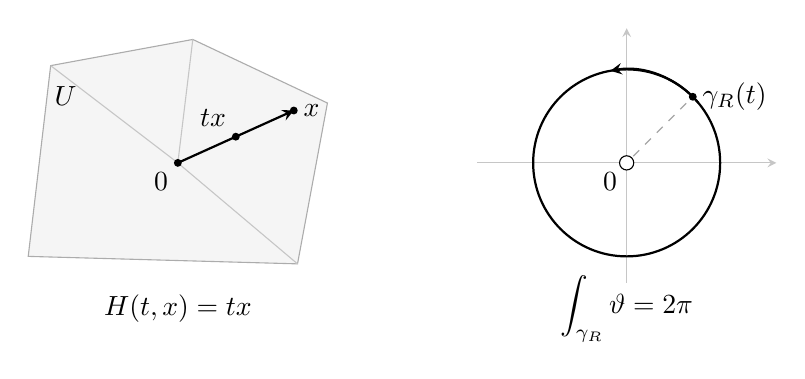
\begin{tikzpicture}[>=stealth,scale=0.95]
		\begin{scope}
			\filldraw[fill=gray!8,draw=gray!65] (-2,-1.25)--(-1.7,1.3)--(0.2,1.65)--(2,0.8)--(1.6,-1.35)--cycle;
			\node at (-1.5,0.9) {\(U\)};
			\draw[gray!45] (0,0)--(-1.7,1.3);
			\draw[gray!45] (0,0)--(0.2,1.65);
			\draw[gray!45] (0,0)--(1.6,-1.35);
			\draw[thick,->] (0,0)--(1.55,0.7);
			\fill (0,0) circle (1.5pt) node[below left] {\(0\)};
			\fill (0.775,0.35) circle (1.5pt) node[above left] {\(tx\)};
			\fill (1.55,0.7) circle (1.5pt) node[right] {\(x\)};
			\node at (0,-1.95) {\(H(t,x)=tx\)};
		\end{scope}
		\begin{scope}[xshift=6cm]
			\draw[gray!45,->] (-2,0)--(2,0);
			\draw[gray!45,->] (0,-1.6)--(0,1.8);
			\draw[thick] (0,0) circle (1.25);
			\draw[thick,->] (40:1.25) arc (40:100:1.25);
			\draw[dashed,gray!70] (0.09,0.09)--(45:1.25);
			\filldraw[fill=white,draw=black] (0,0) circle (2.7pt);
			\node[below left] at (0,0) {\(0\)};
			\fill (45:1.25) circle (1.5pt);
			\node[right] at (45:1.25) {\(\gamma_R(t)\)};
			\node at (0,-1.95) {\(\displaystyle\int_{\gamma_R}\vartheta=2\pi\)};
		\end{scope}
	\end{tikzpicture}
	\caption{左图中，从 \(0\) 到 \(x\) 的径向路径始终留在星形区域内，因此可以沿这一族路径构造原形式。右图的原点被删去，径向收缩不能到达原点；角形式沿圆周的非零周期进一步证明它没有整体原函数。}
	\label{g1:fig:radial-and-period}
\end{figure}


\cref{g1:fig:radial-and-period}把两种构造放在一起：星形区域中径向同伦始终留在定义域内，而穿孔平面中不能把终点设为被删除的原点。穿孔平面上的非恰当性由上面的周期计算证明，不能仅凭一个选定的径向构造失效便作判断。

\ProseParagraphBreak

将角形式限制到单位圆周也得到一个反例。以下取 \(S^1=\{(x,y):x^2+y^2=1\}\)，令 \(j:S^1\hookrightarrow P\) 为包含映射，并记
\[
	\sigma=j^*\vartheta,\qquad
	q:\mathbb R\longrightarrow S^1,\quad q(t)=(\cos t,\sin t).
\]
于是 \(q^*\sigma=\mathrm{d}t\)，沿正向一周的周期为 \(2\pi\)，故 \(\sigma\) 在圆周上不恰当。圆周上的每个一形式都闭，因为二次形式空间为零；所以在一维流形上，闭性本身也不能消除绕圈后的整体障碍。

\begin{proposition}[圆周上的周期判据]
	\label{g1:prop:circle-exactness-period}
	设 \(\lambda\) 为单位圆周 \(S^1\) 上的光滑一形式，写
	\[
		q^*\lambda=a(t)\,\mathrm{d}t,\qquad
		\mathcal P(\lambda)=\int_0^{2\pi}a(t)\,\mathrm{d}t.
	\]
	则 \(a\) 是光滑的 \(2\pi\) 周期函数，且 \(\lambda\) 恰当当且仅当 \(\mathcal P(\lambda)=0\)。更一般地，每个这样的形式都可写成
	\[
		\lambda=c\sigma+\mathrm{d}u,\qquad
		c=\frac{\mathcal P(\lambda)}{2\pi},
	\]
	其中 \(c\) 唯一，光滑函数 \(u:S^1\to\mathbb R\) 在相差常数的意义下唯一。
\end{proposition}
\begin{proof}
	由于 \(q(t+2\pi)=q(t)\) 且 \(q'(t+2\pi)=q'(t)\)，系数 \(a(t)=\lambda_{q(t)}(q'(t))\) 光滑并具有所述周期。若 \(\lambda=\mathrm{d}u\)，沿 \(q|_{[0,2\pi]}\) 使用\cref{g1:lem:exact-path-period}，得到 \(\mathcal P(\lambda)=0\)。

	反过来，设周期为零，令
	\[
		A(t)=\int_0^t a(s)\,\mathrm{d}s.
	\]
	周期性给出 \(A(t+2\pi)-A(t)=\mathcal P(\lambda)=0\)，所以 \(A\) 也为 \(2\pi\) 周期函数。于是可以定义 \(u(q(t))=A(t)\)：两个实数给出同一圆周点时相差 \(2\pi\) 的整数倍，故这个值与代表无关。

	还须检查下降后的函数光滑。\(q'(t)\) 从不为零，由\cref{g1:thm:inverse-function}，\(q\) 在每点附近到一个圆周小弧是微分同胚；在这个小弧上，\(u\) 就是光滑函数 \(A\) 与光滑局部角坐标的复合。因此 \(u\) 光滑。又有
	\[
		q^*(\mathrm{d}u)=\mathrm{d}(u\circ q)=\mathrm{d}A
		=a(t)\,\mathrm{d}t=q^*\lambda.
	\]
	\(q\) 满射且局部微分同胚，每个圆周切向量都能在某个实数点由其微分得到，所以拉回相等蕴含 \(\mathrm{d}u=\lambda\)。

	对一般 \(\lambda\)，取 \(c=\mathcal P(\lambda)/(2\pi)\)，则 \(\lambda-c\sigma\) 的周期为零，刚才的结论给出所需 \(u\)。若存在另一种分解，取周期便知常系数同为 \(c\)；随后两个原函数之差的微分为零。圆周连通，局部常值结论使它们只差常数。
\end{proof}

例如 \(\sigma\) 没有整体原函数，但 \(x\sigma\) 有：在角参数中，它的拉回为 \(\cos t\,\mathrm{d}t=\mathrm{d}(\sin t)\)，所以 \(x\sigma=\mathrm{d}(y|_{S^1})\)。而 \((1+x)\sigma\) 的周期仍为 \(2\pi\)，不恰当。这里决定能否取整体原函数的是一周累积的周期，而不是形式在某个局部坐标中的系数是否为零。
% 纲要条目排为编号小节标题，并进入目录与书签；说明段仍保留于纲要注释中。

% !TeX root = ../../Book1.tex
% 纲要标题：### 14.3 定向、密度与积分
% 纲要位置：几何学计划纲要.md，第 662 行。
% 正文状态：初稿；尚未正式审核。

% 纲要内容开始
% 
% * 定向线和相容图册
% * 密度及不可定向流形的积分
% * 紧支顶次形式的积分
% * 坐标选择和单位分解无关性
% * 定向映射的换元公式
% 
% 纲要内容结束

\section{定向、密度与积分}
\label{g1:sec:1403}

一个局部公式 \(a(x)\,\mathrm{d}x^1\wedge\cdots\wedge\mathrm{d}x^n\) 很像多元积分中的被积表达式，但换坐标时它带的是行列式，而通常的体积换元带绝对行列式。两者之间的符号差，正是定向要处理的问题。密度保留体积缩放而不保留方向，因此在不可定向流形上也能积分。本节先分清这两种对象，再用单位分解把局部积分拼成整体积分。

\ProseParagraphBreak

本节流形均有限维、Hausdorff、第二可数，可以带边界。积分先对光滑紧支对象定义；非紧流形上的非紧支积分还要另查收敛性。分析方面使用一元微积分基本定理、绝对可积函数的 Fubini 定理，以及下面的欧氏换元定理：若 \(F:U\to V\) 是欧氏开集之间的 \(C^1\) 微分同胚，\(h\) 在 \(V\) 上 Lebesgue 可积，则 \((h\circ F)|\det \mathrm{D}F|\) 在 \(U\) 上可积，且
\begin{equation}\label{g1:eq:euclidean-integration-input}
	\int_U h(F(x))|\det \mathrm{D}F_x|\,\mathrm{d}\lambda(x)=\int_V h(y)\,\mathrm{d}\lambda(y).
\end{equation}
这里 \(\lambda\) 是欧氏体积测度，\(\mathrm{d}\lambda\) 没有定向符号。这些是所调用的多元分析基础，分析背景的阅读位置为\cite[Appendix C, Multiple Integrals, pp. 649--655]{Lee2012Smooth}。在半空间图中，对内部应用这些结果；边界超平面是零测集，因而不影响顶维积分。紧支光滑系数有界，其支集位于有限个有界坐标片内，保证下文所用积分绝对收敛。

\subsection{定向线和相容图册}
\label{g1:subsec:1403:01}

回顾\cref{g1:def:determinant-density-line}：当 \(n\geq1\) 时，有序基之间按换基行列式为正划分为两个定向类。在流形上逐点任选一个类还不够，选择必须在局部保持一致。沿小邻域连续移动一个正向标架时，不能突然把它改称反向。

\begin{definition}
	\label{g1:def:manifold-orientation}
	设 \(M\) 为 \(n\geq1\) 维光滑流形。若在每个 \(\mathrm{T}_pM\) 上选定一个定向，并且每点附近存在在各点都为正向的光滑标架，则称这个选择为 \(M\) 的\term[liuxingdingxiang]{定向}[orientation]。允许这样的选择时称 \(M\) 可定向，连同一个选择时称为定向流形。零维流形的定向约定为在每个点选一个符号 \(\varepsilon_p\in\{1,-1\}\)；它用于给有向端点的积分赋号。
\end{definition}

在坐标图 \(x\) 上，令 \(\varepsilon_x(p)\) 表示坐标标架 \((\partial_{x^1},\ldots,\partial_{x^n})\) 是否正向：正向时为 \(1\)，反向时为 \(-1\)。局部一致性等价于 \(\varepsilon_x\) 局部常值。我们通常把图域取为连通的，于是它是一个常数。在两图重叠处，链式法则给出
\begin{equation}\label{g1:eq:orientation-chart-sign}
	\varepsilon_y=\varepsilon_x\operatorname{sgn}\det\frac{\partial x}{\partial y}.
\end{equation}
在无边界情形，必要时反射一个坐标，便可使每张图都正向；于是定向等价于过渡映射的 Jacobian 行列式均为正的相容图册。对于边界模型 \(x^n\geq0\)，保留带符号的表达更方便。尤其在一维区间右端点，只能用向内增大的半直线坐标，不能既要求它正向又要求其取值非负；\(\varepsilon_x\) 会准确记录这个符号。

\ProseParagraphBreak

还可以把符号的变化组织成一个丛。在每张图上取一个实线生成元 \(o_x\)，在交叠处规定
\[
	o_y=\operatorname{sgn}\det\frac{\partial x}{\partial y}\,o_x.
\]
行列式乘法保证三重交叠的余循环条件，所以\cref{g1:thm:bundle-cocycle-gluing}的粘合构造给出一条实光滑线丛，称为\term[dingxiangxian]{定向线丛}[orientation line bundle]，记为 \(\mathfrak o_M\)。它只记录行列式的符号，与使用整个行列式的行列式线丛不同。定向等价于在此线丛中连续选择 \(\pm o_x\) 的一个：表达为 \(\varepsilon_xo_x\)，\eqref{g1:eq:orientation-chart-sign}恰好保证它在换图后不变。零维时取平凡实线丛，在各点选择其正或负单位元。

\begin{proposition}[定向与顶次形式]
	\label{g1:prop:orientation-nonvanishing-form}
	设 \(M\) 为上述光滑 \(n\) 维流形。\(M\) 可定向当且仅当存在处处非零的光滑 \(n\) 形式。给定定向后，可以选择在每个正向有序基上取正值的顶次形式；零维时这表示函数在每点的符号与所选定向一致。
\end{proposition}
\begin{proof}
	对 \(n\geq1\)，若 \(\nu\) 处处非零，就把满足 \(\nu_p(e_1,\ldots,e_n)>0\) 的基规定为正向。局部坐标中 \(\nu=a(x)\,\mathrm{d}x^1\wedge\cdots\wedge\mathrm{d}x^n\)，系数连续且不为零，其符号局部不变，所以确实给出定向。

	反向，\cref{g1:thm:bundle-metric-existence}在 \(\mathrm{T}M\) 上给出光滑正定度量。每张图内把正向标架作光滑正交归一化，正向正交标架之间的矩阵属于 \(\operatorname{SO}(n)\)，行列式为一。因此各正向正交标架的顶次对偶楔积在交叠处相同，粘成所需 \(\nu\)。这也是\cref{g1:prop:orientation-volume-reductions}用于切丛的具体情形。零维时取函数 \(\nu(p)=\varepsilon_p\)；零维流形离散，故它光滑且处处非零。
\end{proof}

例如开 Möbius 带可写成 \(\mathbb R\times(-1,1)\) 在 \((t,u)\sim(t+1,-u)\) 下的商。若它有非零顶次形式，拉回到条带必为 \(a(t,u)\,\mathrm{d}t\wedge\mathrm{d}u\)，且不变性要求
\[
	a(t+1,-u)=-a(t,u).
\]
在中线上，\(a(t+1,0)=-a(t,0)\)，连续性迫使它在一圈中经过零，矛盾。这里每个小矩形都能定向，阻碍来自绕过整个带后的符号变化。

\subsection{密度及不可定向流形的积分}
\label{g1:subsec:1403:02}

\cref{g1:def:determinant-density-line}把密度定义为有序基上的实值函数，换基时乘 \(|\det A|\)。逐点使用这一构造得到密度线丛 \(\mathcal D(M)=|\Lambda^n\mathrm{T}^*M|\)。在坐标图中，光滑密度写为
\[
	\mu=m_x(x)\,|\mathrm{d}x^1\cdots\mathrm{d}x^n|,
\]
换成 \(y\) 坐标后，系数满足
\begin{equation}\label{g1:eq:density-coordinate-change}
	m_y(y)=m_x(x(y))\left|\det\frac{\partial x}{\partial y}\right|.
\end{equation}
系数可以为负，密度线仍是实线性空间；正密度才要求 \(m_x>0\)。若一条光滑密度的支集紧且包含于图域 \(U\)，定义它在该图中的积分为
\[
	I_x(\mu)=\int_{x(U)}m_x(x)\,\mathrm{d}\lambda(x).
\]
由\eqref{g1:eq:density-coordinate-change}和欧氏换元公式，这个数在另一张包含支集的图中不变。这里恰好需要绝对行列式，所以不必指定两图是否同向。

\ProseParagraphBreak

若支集不能放在一张图里，选从属于坐标覆盖的非负光滑单位分解 \(\{\rho_i\}\)，并取 \(\operatorname{supp}\rho_i\subset U_i\)。设 \(\mu\) 紧支，则 \(\rho_i\mu\) 的支集是 \(U_i\) 中的紧集。局部有限性还使只有有限个 \(\rho_i\mu\) 不为零：用有限个局部有限邻域覆盖 \(\operatorname{supp}\mu\)，它们总共只遇到有限个支集。于是可以提出整体积分的定义
\begin{equation}\label{g1:eq:density-integral-definition}
	\int_M\mu=\sum_i I_{x_i}(\rho_i\mu).
\end{equation}
这项和式与单位分解无关的证明，将与顶次形式一起在\subsecref{g1:subsec:1403:04}给出；目前求和的各项和有限性都已经有定义。

\begin{example}[Möbius 带上的面积]
	\label{g1:exm:mobius-density-integral}
	在闭条带 \(\mathbb R\times[-1,1]\) 的上述商上，\(|\mathrm{d}t\,\mathrm{d}u|\) 被变换 \((t,u)\mapsto(t+1,-u)\) 保持，因此下降为正光滑密度。用 \(0\leq t\leq1\)、\(-1\leq u\leq1\) 作基本区域，其积分为 \(2\)。计算时可以把基本区域划成落在商坐标图中的小矩形；公共边以及识别的两条竖边都是二维零测集，不会被重复计入面积。带边界的这个 Möbius 带仍不可定向，因为前面的中线论证不变，却有良定义的面积。
\end{example}

密度解决了测量体积的问题，却不自行产生一个与外微分相容的带符号边界公式。后面的 Stokes 定理仍对定向流形上的微分形式陈述，不能因密度总能积分就删去定向条件。

\subsection{紧支顶次形式的积分}
\label{g1:subsec:1403:03}

现在给 \(M\) 选定定向。若 \(\omega\in\Omega_c^n(M)\) 的支集在一个连通图域 \(U\) 中，并写成
\[
	\omega=a_x(x)\,\mathrm{d}x^1\wedge\cdots\wedge\mathrm{d}x^n,
\]
定义
\begin{equation}\label{g1:eq:oriented-chart-integral}
	I_x^{\mathrm{or}}(\omega)=\varepsilon_x\int_{x(U)}a_x(x)\,\mathrm{d}\lambda(x).
\end{equation}
在正向图中 \(\varepsilon_x=1\)，得到熟悉的公式；反向图中要额外乘 \(-1\)。这不是对被积系数取绝对值，形式的积分可以为负，也可以因正负部分抵消而为零。

\ProseParagraphBreak

对一般紧支顶次形式，以从属于坐标覆盖的单位分解规定
\begin{equation}\label{g1:eq:top-form-integral-definition}
	\int_M\omega=\sum_i I_{x_i}^{\mathrm{or}}(\rho_i\omega).
\end{equation}
和式仍只有有限个非零项。零维流形上的紧集只有有限个点，此时 \(0\) 形式就是函数，定义专门写为
\[
	\int_M f=\sum_{p\in M}\varepsilon_p f(p),
\]
其中紧支性保证求和有限。特别地，一个正向点的积分为函数值，负向点的积分为其相反数。这将使区间的两个边界端点分别贡献 \(f(b)\) 与 \(-f(a)\)。

\ProseParagraphBreak

定向也给出顶次形式到密度的线性对应。令 \(S_o\omega\) 在 \(x\) 图中的密度系数为 \(\varepsilon_xa_x\)。因为
\[
	a_y=a_x\det\frac{\partial x}{\partial y},\qquad
	\varepsilon_y=\varepsilon_x\operatorname{sgn}\det\frac{\partial x}{\partial y},
\]
乘积 \(\varepsilon_ya_y\) 恰按绝对行列式变换，所以这些局部系数粘成密度。这与非线性的 \(|\omega|\) 不同：\(S_o\omega\) 保留相对于给定定向的正负号，\(|\omega|\) 只保留绝对大小。由局部定义，\(\int_M\omega=\int_M S_o\omega\)。反转定向时 \(S_o\) 变号，故形式积分也变号，密度积分本身则不变。

\subsection{坐标选择和单位分解无关性}
\label{g1:subsec:1403:04}

\begin{theorem}[流形积分的良定义性]
	\label{g1:thm:integral-well-defined}
	设 \(M\) 为有限维、Hausdorff、第二可数光滑流形，允许边界。\eqref{g1:eq:density-integral-definition}对每个紧支光滑密度定义一个与坐标覆盖和从属单位分解无关的实数。若另给定向，则\eqref{g1:eq:top-form-integral-definition}对每个紧支光滑顶次形式也有同样性质。两种积分均线性；非负且不恒为零的光滑密度积分严格为正。
\end{theorem}
\begin{proof}
	密度在一张图中的积分已经由欧氏换元证明与图无关。形式也如此：在两个图的交中，其系数相差有符号行列式，图的定向符号满足\eqref{g1:eq:orientation-chart-sign}。两者相乘得到绝对行列式，故
	\[
		\varepsilon_y\int a_y\,\mathrm{d}\lambda(y)
		=\varepsilon_x\int a_x(x(y))\left|\det\frac{\partial x}{\partial y}\right|\mathrm{d}\lambda(y)
		=\varepsilon_x\int a_x\,\mathrm{d}\lambda(x).
	\]
	若交集不连通，对各连通分支使用相同公式，或直接把局部常值符号保留在被积函数中。边界图的换元在内部进行，边界零测不改变结果。

	现取两套从属于坐标覆盖的单位分解 \(\{\rho_i\}\)、\(\{\sigma_j\}\)，图分别记为 \(x_i,y_j\)。令 \(u\) 表示待积的密度或顶次形式。只有有限个支集与 \(\operatorname{supp}u\) 相交，因此下面实为有限次拆分：
	\[
		\sum_i I_{x_i}(\rho_i u)
		=\sum_{i,j}I_{x_i}(\rho_i\sigma_j u)
		=\sum_{i,j}I_{y_j}(\rho_i\sigma_j u)
		=\sum_j I_{y_j}(\sigma_j u).
	\]
	形式情形中的 \(I\) 理解为 \(I^{\mathrm{or}}\)。中间每个对象的支集紧且包含在 \(U_i\cap V_j\) 中，所以第一步的单图换元确实适用。最外两次等式分别使用 \(\sum_j\sigma_j=1\)、\(\sum_i\rho_i=1\)，并利用欧氏积分的线性。由此同时排除了覆盖、坐标与单位分解的选择依赖。

	线性可以在同一套覆盖和单位分解中逐项验证。若 \(\mu\geq0\) 且某点处严格为正，连续性给出某张图内的一块区域，其系数有正下界。该点处至少一个 \(\rho_i>0\)，缩小区域后 \(\rho_i\mu\) 的系数仍有正下界，因此这一项积分正，其余项非负。边界点附近可取正体积的半球内部，零维时则是一项正数。这证明严格正性。
\end{proof}

证明中的共同细化 \(\rho_i\sigma_j\) 是关键：不必在两套坐标之间直接比较整个和式，只需把它们拆成同时落在两张图中的小块。局部有限性让这一分解在紧支集上化为有限运算，避免了任何未经说明的无穷级数换序。

\begin{proposition}[度量的体积积分]
	\label{g1:prop:metric-volume-integration}
	设 \(g\) 为 \(M^n\) 上的光滑正定度量。其正体积密度在坐标中为
	\[
		\mu_g=\sqrt{\det(g_{ij})}\,|\mathrm{d}x^1\cdots\mathrm{d}x^n|.
	\]
	若 \(M\) 定向，则相应的正体积形式为
	\[
		\operatorname{vol}_g=\varepsilon_x\sqrt{\det(g_{ij})}\,\mathrm{d}x^1\wedge\cdots\wedge\mathrm{d}x^n,
	\]
	并且对每个紧支光滑函数 \(f\)，有 \(\int_M f\operatorname{vol}_g=\int_M f\mu_g\)。
\end{proposition}
\begin{proof}
	\cref{g1:prop:gram-volume-density}在每个切空间给出 \(\mu_g(e)=\sqrt{\det[g(e_i,e_j)]}\)，取坐标标架就得到密度公式；正定性使行列式正，其正平方根随点光滑。把坐标标架的定向符号乘入顶次形式，便使其在正向标架上取正值，且换图时相容。最后 \(S_o(f\operatorname{vol}_g)\) 的局部系数为 \(f\sqrt{\det(g_{ij})}\)，正是 \(f\mu_g\)，所以积分相同。
\end{proof}

例如平面的极坐标在 \(r>0\) 的角度分支上给出 \(g=\mathrm{d}r^2+r^2\mathrm{d}\theta^2\)，所以体积密度为 \(r|\mathrm{d}r\,\mathrm{d}\theta|\)。\(r=0\) 不是这张坐标图的一点，不能把极坐标表达在原点的退化误认为欧氏度量退化。对半径为 \(R\) 的圆盘积分得到 \(\int_0^{2\pi}\int_0^R r\,\mathrm{d}r\,\mathrm{d}\theta=\pi R^2\)；被忽略的中心及切开的射线面积为零。

\subsection{定向映射的换元公式}
\label{g1:subsec:1403:05}

对任意光滑映射都能拉回微分形式，但积分的简单换元公式首先适用于微分同胚。非单射映射可能重复覆盖区域，微分降秩也可能压缩维数；这些情况不能仅凭拉回有定义就沿用同一个积分等式。

\begin{theorem}[定向换元]
	\label{g1:thm:oriented-change-variables}
	设 \(F:M^n\to N^n\) 为光滑流形之间的微分同胚，允许边界。
	\begin{enumerate}
		\item 对 \(N\) 上的紧支光滑密度 \(\mu\)，其微分同胚拉回满足 \(\int_M F^*\mu=\int_N\mu\)。
		\item 若两流形定向，定义 \(s_F(p)=1\) 当 \(\mathrm{d}F_p\) 保定向，反向时为 \(-1\)。则 \(s_F\) 局部常值，且对任意 \(\omega\in\Omega_c^n(N)\)，
		\[
			\int_M F^*\omega=\int_N(s_F\circ F^{-1})\omega.
		\]
		特别地，整体保定向时积分不变，整体反定向时积分变号。若 \(M\) 连通，符号只有上述两种整体可能。
	\end{enumerate}
	零维时，用源点和像点的定向符号之比定义 \(s_F\)，同一公式成立。
\end{theorem}
\begin{proof}
	微分同胚将紧集的原像变为紧集，所以两种拉回仍紧支。对目标支集选有限个所需坐标片及从属单位分解，再拉回到源；它们的拉回仍构成从属单位分解。故只需证明单图的结果。

	在源图 \(x\) 和目标图 \(y\) 中，记 \(G=y\circ F\circ x^{-1}\)。若 \(\mu=m(y)|\mathrm{d}y^1\cdots\mathrm{d}y^n|\)，则其拉回系数为 \(m(G(x))|\det \mathrm{D}G_x|\)，欧氏换元直接给出第一项。若 \(\omega=a(y)\,\mathrm{d}y^1\wedge\cdots\wedge\mathrm{d}y^n\)，则拉回系数为 \(a(G(x))\det \mathrm{D}G_x\)。源、目标图的定向符号分别为 \(\varepsilon_x,\varepsilon_y\)，有
	\[
		s_F=\varepsilon_x\varepsilon_y\operatorname{sgn}\det \mathrm{D}G,
	\]
	所以 \(\varepsilon_x\det \mathrm{D}G=s_F\varepsilon_y|\det \mathrm{D}G|\)。代入单图积分，再用欧氏换元，便得到第二项；逐片相加完成证明。符号的局部常值性来自非零行列式的连续性，在连通流形上因此恒定。零维公式就是把有限项求和按双射重新编号。
\end{proof}

以反射 \(F(x^1,x^2)=(-x^1,x^2)\) 为例，在标准定向的平面上，\(F^*(a\,\mathrm{d}x^1\wedge\mathrm{d}x^2)=-a(-x^1,x^2)\,\mathrm{d}x^1\wedge\mathrm{d}x^2\)，故紧支形式的积分变号；密度的拉回则没有这个负号。又如圆周映射 \(e^{\mathrm{i}\theta}\mapsto e^{2\mathrm{i}\theta}\) 不是微分同胚，它把角形式拉回为两倍，积分也变成两倍。后者涉及重复覆盖次数，将在\secref{g1:sec:1405}进一步说明，不能当作当前换元定理的一个无条件推论。

% 纲要条目排为编号小节标题，并进入目录与书签；说明段仍保留于纲要注释中。

% !TeX root = ../../Book1.tex
% 纲要标题：### 14.4 边界定向与 Stokes 的证明
% 纲要位置：几何学计划纲要.md，第 670 行。
% 正文状态：初稿；尚未正式审核。

% 纲要内容开始
% 
% * 外法向优先的边界约定
% * 半空间中的局部公式
% * 通过单位分解粘合
% * 带角区域及逐项边界符号
% * Green、Gauss 公式作为特例
% 
% 纲要内容结束

\section{边界定向与 Stokes 的证明}
\label{g1:sec:1404}

在一元微积分中，导数的积分只留下区间两个端点的函数值，而且右端点取正号、左端点取负号。Stokes 定理把这个关系推广到微分形式：区域内部的外微分积分，等于边界上原形式的积分。这里“边界”必须带有由区域定向确定的方向，否则等式连符号都不能确定。

\ProseParagraphBreak

第九章已经在曲面坐标中证明了所需的 Green 公式，并据此把联络形式的边界积分换成曲率积分，见\cref{g1:lem:green-formula,g1:thm:local-gauss-bonnet}。本节从同一个积分基本定理出发，先处理任意维半空间，再用第十二章的光滑单位分解得到整体公式。所有形式都光滑至边界；非紧流形上的形式要求紧支，支集可以接触实际边界。

\subsection{外法向优先的边界约定}
\label{g1:subsec:1404:01}

设 \(M^n\) 为有向带边界光滑流形，\(n\ge1\)，包含映射记为 \(j:\partial M\hookrightarrow M\)。\cref{g1:prop:boundary-chart-invariance}说明，\(\partial M\) 本身是 \(n-1\) 维无边界光滑流形；其完整切空间由边界坐标中最后一个分量为零的向量组成。若在边界图中把 \(M\) 写成 \(x^n\ge0\)，则指向外侧的横截向量满足 \(\mathrm{d}x^n(\nu)<0\)。这个描述只用边界两侧的区分，不需要长度或正交关系。

\begin{definition}[边界定向]\label{g1:def:boundary-orientation}
	设 \(M^n\) 为有向带边界光滑流形，\(n\ge1\)。在 \(p\in\partial M\) 取一个外向横截向量 \(\nu\)，即在边界定义坐标 \(\rho\ge0\) 下满足 \(\mathrm{d}\rho_p(\nu)<0\)。边界取\term[waifaxiangyouxian]{外法向优先}[outward-normal-first]的定向：当 \(n\ge2\) 时，基 \((v_1,\ldots,v_{n-1})\) 在 \(\mathrm{T}_p\partial M\) 中为正向，当且仅当
	\[
		(\nu,v_1,\ldots,v_{n-1})
	\]
	在 \(\mathrm{T}_pM\) 中为正向。等价地，若 \(\Omega_p\) 是表示 \(M\) 正定向的非零顶次协变向量，则 \((\iota_\nu\Omega_p)|_{\mathrm{T}_p\partial M}\) 表示边界的正定向。后一表述也适用于 \(n=1\)：它给边界点指定一个正负号。
\end{definition}

名称中的“法向”只指横截方向；若另有黎曼度量，才可以特选外向单位法向。先核对这个约定不依赖选择。两种边界定义坐标 \(\rho,\rho'\) 在边界上都为零，局部可写成
\[
	\rho'=\rho\,a,\qquad
	a(x',\rho)=\int_0^1\partial_\rho\rho'(x',t\rho)\,\mathrm{d}t.
\]
边界坐标变换可逆，且把内侧映到内侧，所以 \(a(p)>0\)：其边界处的法向导数不为零，又不能为负。这也可由\cref{g1:prop:boundary-smooth-derivative}的链式法则和一侧非负性直接判断。因此 \(\mathrm{d}\rho'_p=a(p)\mathrm{d}\rho_p\)，外向条件与坐标无关。

\ProseParagraphBreak

若 \(\nu,\nu'\) 都外向，则在一维商空间 \(\mathrm{T}_pM/\mathrm{T}_p\partial M\) 中，它们位于同一条半直线上，故
\[
	\nu'=c\nu+w,\qquad c>0,\quad w\in \mathrm{T}_p\partial M.
\]
把第一列由 \(\nu\) 换为 \(\nu'\)，行列式只乘以正数 \(c\)，因为 \(w\) 是其余切向列的线性组合。等价地，插入 \(w\) 后限制到边界切空间的顶次形式为零。因此边界定向与外向横截向量及正顶次形式的选择无关，且随点光滑变化。

在标准定向半空间
\[
	H^n=\{x^n\ge0\},\qquad
	\Omega=\mathrm{d}x^1\wedge\cdots\wedge\mathrm{d}x^n
\]
中，可以取 \(\nu=-\partial_{x^n}\)。于是
\begin{equation}\label{g1:eq:half-space-boundary-orientation}
	\left.\iota_{-\partial_{x^n}}\Omega\right|_{\partial H^n}
	=(-1)^n\,\mathrm{d}x^1\wedge\cdots\wedge\mathrm{d}x^{n-1}.
\end{equation}
所以边界坐标 \((x^1,\ldots,x^{n-1})\) 的通常定向，与诱导边界定向相差 \((-1)^n\)。这个符号来自把最后一个坐标向量移到第一位，再乘上外向向量的负号。

\ProseParagraphBreak

当 \(n=1\) 时，标准半直线的边界点 \(0\) 取负号；对按递增参数定向的区间 \([a,b]\)，左端点取负、右端点取正。按照上一节的有向零维积分约定，
\[
	\int_{\partial[a,b]}f=f(b)-f(a).
\]
零维流形另约定边界为空，不再应用“降低一维”的基向量描述。此时没有需要讨论的负一次形式；若记 \(\Omega^{-1}=0\)，Stokes 等式只表示 \(0=0\)。

\subsection{半空间中的局部公式}
\label{g1:subsec:1404:02}

高维公式的局部计算只多了一个排列符号。把一般 \(n-1\) 次形式按“缺少哪个坐标微分”分组，并在第 \(i\) 项预先放入 \((-1)^{i-1}\)，可以让外微分后的各项都具有相同正号。以下用帽子表示删去相应因子。

\begin{lemma}[半空间中的 Stokes 公式]\label{g1:lem:half-space-stokes}
	设 \(n\ge1\)，\(H^n=\{x^n\ge0\}\) 取标准定向，边界取外法向优先定向。若 \(\alpha\) 是 \(H^n\) 上光滑至边界的紧支 \(n-1\) 次形式，则
	\[
		\int_{H^n}\mathrm{d}\alpha=\int_{\partial H^n}j^*\alpha.
	\]
	在无边界模型 \(\mathbb R^n\) 上，任意紧支光滑 \(n-1\) 次形式都满足 \(\int_{\mathbb R^n}\mathrm{d}\alpha=0\)。紧支集允许与 \(x^n=0\) 相交。
\end{lemma}
\begin{proof}
	唯一写成
	\[
		\alpha=\sum_{i=1}^n(-1)^{i-1}a_i(x)\,
		\mathrm{d}x^1\wedge\cdots\wedge\widehat{\mathrm{d}x^i}\wedge\cdots\wedge\mathrm{d}x^n.
	\]
	每个 \(a_i\) 光滑且紧支。由\cref{g1:thm:exterior-derivative}的坐标公式，求外微分时，只有 \(\partial_i a_i\,\mathrm{d}x^i\) 那一项不因重复微分而消失。把 \(\mathrm{d}x^i\) 移到第 \(i\) 位又产生 \((-1)^{i-1}\)，两个符号抵消，故
	\begin{equation}\label{g1:eq:stokes-local-divergence}
		\mathrm{d}\alpha=\left(\sum_{i=1}^n\partial_i a_i\right)
		\mathrm{d}x^1\wedge\cdots\wedge\mathrm{d}x^n.
	\end{equation}

	取 \(R\) 足够大，使全部系数支集位于 \((-R,R)^{n-1}\times[0,R)\)。连续系数及其导数在这个紧盒上可积，累次积分的 Fubini 公式允许先沿任一坐标积分。对 \(i<n\)，沿 \(x^i\) 的积分区间两端，\(a_i\) 都为零，所以
	\[
		\int_{H^n}\partial_i a_i\,\mathrm{d}x=0.
	\]
	最后一个坐标则从零开始，积分基本定理给出
	\[
		\int_{H^n}\partial_n a_n\,\mathrm{d}x
		=-\int_{\mathbb R^{n-1}}a_n(x',0)\,\mathrm{d}x'.
	\]
	因此体积分只留下这一个负的边界值。

	在边界上拉回时，含 \(\mathrm{d}x^n\) 的项全部消失，故
	\[
		j^*\alpha=(-1)^{n-1}a_n(x',0)\,
		\mathrm{d}x^1\wedge\cdots\wedge\mathrm{d}x^{n-1}.
	\]
	但边界的定向符号还要乘上\eqref{g1:eq:half-space-boundary-orientation}中的 \((-1)^n\)。于是
	\[
		\int_{\partial H^n}j^*\alpha
		=(-1)^n(-1)^{n-1}\int_{\mathbb R^{n-1}}a_n(x',0)\,\mathrm{d}x'
		=-\int_{\mathbb R^{n-1}}a_n(x',0)\,\mathrm{d}x',
	\]
	恰与体积分相同。\(n=1\) 时，右侧按零维积分解释为 \(-a_1(0)\)，同样成立。

	在 \(\mathbb R^n\) 上，每个坐标都在完整实轴上积分，紧支性使各方向两端的系数为零，故所有偏导积分都为零。
\end{proof}

这里没有把 \(\alpha\) 越过实际边界 \(x^n=0\) 补成零。那样补零通常不光滑，而且会错误地抹掉边界项。紧支性只保证在足够远的辅助截断边缘处系数为零，真正的边界值 \(a_n(x',0)\) 完整保留。

\subsection{通过单位分解粘合}
\label{g1:subsec:1404:03}

\begin{theorem}[Stokes 定理]\label{g1:thm:stokes}
	设 \(M^n\) 为有限维、Hausdorff、第二可数的有向光滑流形，允许有边界，\(n\ge1\)。给 \(\partial M\) 外法向优先定向，记包含映射为 \(j\)。对每个紧支光滑 \(n-1\) 次形式 \(\omega\in\Omega_c^{n-1}(M)\)，有
	\begin{equation}\label{g1:eq:stokes}
		\int_M\mathrm{d}\omega=\int_{\partial M}j^*\omega.
	\end{equation}
	此式称为\term[stokesdingli]{Stokes 定理}[Stokes theorem]。不要求 \(M\) 紧；若 \(M\) 紧，则任意光滑 \(n-1\) 次形式自动满足支集条件。
\end{theorem}
\begin{proof}
	令 \(K=\operatorname{supp}\omega\)。在 \(M\setminus K\) 的每个点附近，\(\omega\) 恒为零，故 \(\operatorname{supp}\mathrm{d}\omega\subseteq K\)。由于边界是闭集，\(j^*\omega\) 的支集包含于紧集 \(K\cap\partial M\)。因此两边的积分均在上一节已定义的紧支积分范围内。

	用内部坐标图和边界坐标图覆盖 \(M\)，再由\cref{g1:thm:smooth-partition-unity}取从属光滑单位分解 \(\{\rho_i\}\)。局部有限的支集族只会有有限个成员与紧集 \(K\) 相交：给 \(K\) 中每一点选一个只遇到有限个支集的邻域，再从这些邻域取有限子覆盖即可。因此
	\[
		\omega=\sum_i\omega_i,\qquad \omega_i=\rho_i\omega
	\]
	实际上只有有限个非零项；每个 \(\omega_i\) 的支集是位于对应图域 \(U_i\) 内的紧集。

	将 \(\omega_i\) 写入坐标。其坐标支集紧含于相对开图域，故可越过这个图域的人为边缘补零到整个 \(\mathbb R^n\) 或 \(H^n\)，而保持光滑；补零没有越过 \(H^n\) 的实际边界。由\cref{g1:prop:exterior-pullback}，坐标拉回与外微分交换。对补零形式应用\cref{g1:lem:half-space-stokes}，再用\cref{g1:thm:oriented-change-variables}把积分搬回，便得
	\[
		\int_M\mathrm{d}\omega_i=\int_{\partial M}j^*\omega_i.
	\]
	这里任一图都可以带有定向符号 \(\varepsilon_i=\pm1\)：若坐标参数化反向，体积分和它诱导的边界积分同时乘以 \(-1\)，所以局部等式仍成立。特别是在一维右端点附近，无须强行要求到标准半直线的坐标正向。

	最后把有限个等式相加。注意局部公式作用于 \(\mathrm{d}(\rho_i\omega)\)，而不是直接作用于 \(\rho_i\mathrm{d}\omega\)；乘积法则产生的项正好消去：
	\[
		\begin{aligned}
			\sum_i\mathrm{d}(\rho_i\omega)
			&=\sum_i\mathrm{d}\rho_i\wedge\omega+\sum_i\rho_i\,\mathrm{d}\omega\\
			&=\mathrm{d}\!\left(\sum_i\rho_i\right)\wedge\omega+\mathrm{d}\omega
			=\mathrm{d}\omega.
		\end{aligned}
	\]
	这些等式可先按局部有限和理解，而乘上 \(\omega\) 后只有前述有限个非零项。边界上的和同样为 \(j^*\omega\)。积分的线性及\cref{g1:thm:integral-well-defined}的坐标、单位分解无关性遂给出\eqref{g1:eq:stokes}。
\end{proof}

若 \(M\) 无边界，结论是 \(\int_M\mathrm{d}\omega=0\)；若 \(M=[a,b]\)，结论就是积分基本定理。非紧情形的紧支要求控制了“远处的边界”：仅仅知道 \(\mathrm{d}\omega\) 的积分收敛，并不能保证无穷远没有留下额外项，习题中会给出一维例子。

\subsection{带角区域及逐项边界符号}
\label{g1:subsec:1404:04}

矩形和单形在角点处不具有半空间局部模型。这里先明确所讨论的对象，再把局部公式推广到正交象限；角棱不贡献新的积分项，但邻接的每张面都必须保留。

\begin{definition}[带角流形]\label{g1:def:manifold-with-corners}
	一个 \(n\) 维\term[daijiaoliuxing]{带角流形}[manifold with corners]是 Hausdorff、第二可数空间，带有到
	\[
		Q_k^n=[0,\infty)^k\times\mathbb R^{n-k},
		\qquad 0\le k\le n
	\]
	的相对开集的坐标图；换坐标及其逆都要求局部延拓为欧氏空间中的光滑映射。函数、微分形式和定向也按这种局部延拓定义。在一点附近，只保留在那里取零的受限坐标，其个数称为该点的深度；深度一部分是光滑的余维一边界，深度至少二的部分称为角棱。
\end{definition}

这个深度与坐标无关。像第十一章半空间的论证一样，局部延拓的导数由内部稠密性唯一确定，互逆变换的导数互逆。在深度 \(k\) 的点，单侧曲线的速度构成锥
\[
	C_p=\{v:v^1,\ldots,v^k\ge0\},
\]
其最大线性子空间 \(C_p\cap(-C_p)\) 的维数为 \(n-k\)。坐标变换的微分把这个速度锥同构到目标的速度锥，因此保持 \(k\)。深度一部分在小坐标邻域内分成 \(k\) 张局部面 \(x^i=0\) 的内部；换坐标保持深度，并把这些连通的局部面分支一一对应。每张面的定向先在深度一点由外法向优先确定，再连续延伸到它的角棱。

\ProseParagraphBreak

顶次积分沿用上一节的坐标定义。正交象限中边界在 \(n\) 维测度下为零，不影响体积分；对每张余维一面，角棱在该面内的 \(n-1\) 维测度也为零，因为它们在面坐标中是一个或多个坐标取零的集合。因此边界积分按每张局部面分别计算，同一角点邻接的不同面各计一次，而不把整个拓扑边界误认为一张光滑流形。

\ProseParagraphBreak

这些面上的积分与坐标选择相容：在深度一部分应用有向换元公式即可。若某积分的支集接触角棱，可以先去掉面坐标中宽度为 \(\varepsilon\) 的角棱条带，再令 \(\varepsilon\downarrow0\)。在所用紧坐标片内，形式系数与换元 Jacobian 有界，条带体积趋于零，遗漏积分的绝对值也趋于零。于是普通换元公式延续到接触角棱的积分。用有限坐标分解求和时，两种分解可通过权重乘积作共同细化，逐面利用换元和权重总和为 \(1\)，证明边界积分不依赖分解。以下的 \(\int_{\partial M}\omega\) 就表示这种按局部面分支计算的积分；面上的形式均指包含拉回。

\begin{theorem}[带角流形上的 Stokes 公式]\label{g1:thm:stokes-corners}
	设 \(M^n\) 为有向、Hausdorff、第二可数的光滑带角流形，\(n\ge1\)，\(\omega\) 为光滑至各面的紧支 \(n-1\) 次形式。各余维一面取外法向优先定向，边界积分按局部面分支计算，则
	\[
		\int_M\mathrm{d}\omega=\int_{\partial M}\omega.
	\]
	余维至少二的角棱不增加独立积分项。
\end{theorem}
\begin{proof}
	先在标准定向的 \(Q_k^n\) 上取紧支形式
	\[
		\alpha=\sum_{i=1}^n(-1)^{i-1}a_i\,
		\mathrm{d}x^1\wedge\cdots\wedge\widehat{\mathrm{d}x^i}\wedge\cdots\wedge\mathrm{d}x^n.
	\]
	外微分仍由\eqref{g1:eq:stokes-local-divergence}给出。对不受限坐标 \(i>k\)，偏导积分为零；对 \(i\le k\)，沿 \([0,\infty)\) 使用积分基本定理，得到
	\[
		\int_{Q_k^n}\mathrm{d}\alpha
		=-\sum_{i=1}^k\int_{F_i}a_i|_{x^i=0}\,\mathrm{d}x^{\widehat i},
		\qquad F_i=Q_k^n\cap\{x^i=0\}.
	\]
	这里右侧暂按其余坐标的递增次序使用通常正测度。面 \(F_i\) 的外向向量为 \(-\partial_{x^i}\)，所以相对于这组面坐标，诱导定向的符号为 \((-1)^i\)。拉回 \(\alpha\) 后只留下 \((-1)^{i-1}a_i\,\mathrm{d}x^{\widehat i}\)，两者相乘正好是 \(-a_i\,\mathrm{d}x^{\widehat i}\)。因此上式就是各有向面的积分之和。各坐标面的相交部分测度为零，不会在这个计算之外再留下角点项。

	现在令 \(K=\operatorname{supp}\omega\)。紧集附近只需有限个坐标截断函数。具体地，在每点的带角坐标中取两层相对球，把\cref{g1:lem:smooth-bump-function}中的欧氏截断函数限制到正交象限，得到支集紧含于外层图域、在内层为 \(1\) 的光滑函数。选有限个内层覆盖 \(K\)，记对应函数为 \(b_1,\ldots,b_N\)。其和 \(b\) 在 \(K\) 的开邻域 \(W\) 上为正，令 \(\rho_i=b_i/b\) 于 \(W\)。于是 \(\sum_i\rho_i=1\) 于 \(W\)。

	在 \(W\) 上取 \(\omega_i=\rho_i\omega\)，再在 \(M\setminus W\) 补零。因为 \(K\subset W\)，每个补零位置附近 \(\omega\) 本来就为零，故 \(\omega_i\) 光滑；其支集位于 \(K\cap\operatorname{supp}b_i\)，是相应图域内的紧集。对各 \(\omega_i\) 使用刚证的象限公式，按图的定向符号搬回，并把有限个等式相加。由 \(\sum_i\omega_i=\omega\)，或等价地由 \(\sum_i\mathrm{d}\rho_i=0\) 于 \(W\)，得到所需整体等式。
\end{proof}

如果一个区域由有限个这样的有向块拼成，并且相邻块沿完整面光滑贴合，就对每块应用公式再相加。公共面的外向横截方向对两块相反，而环境定向相同，所以两次诱导面定向相反，内部面项抵消。这里先按面在各块中出现的次数计入，再作抵消；不能一开始就把同一个几何面只算一次。

\ProseParagraphBreak

对按 \((x^1,\ldots,x^n)\) 定向的矩形 \(R=\prod_{i=1}^n[a_i,b_i]\)，记 \(R_{\widehat i}\) 为删去第 \(i\) 个坐标的矩形，取其剩余坐标递增次序的定向；令 \(\delta_i^+,\delta_i^-\) 分别插入 \(x^i=b_i,a_i\)。上面的向量次序给出：上侧面的外向向量为 \(+\partial_{x^i}\)，符号为 \((-1)^{i-1}\)；下侧面的外向向量为 \(-\partial_{x^i}\)，符号为 \((-1)^i\)。于是
\begin{equation}\label{g1:eq:rectangle-boundary-signs}
	\int_{\partial R}\omega
	=\sum_{i=1}^n(-1)^{i-1}\left(
		\int_{R_{\widehat i}}(\delta_i^+)^*\omega
		-\int_{R_{\widehat i}}(\delta_i^-)^*\omega
	\right).
\end{equation}
若把 \(\omega\) 写成前面的 \(\sum_i(-1)^{i-1}a_i\,\mathrm{d}x^{\widehat i}\)，两组排列符号抵消，留下的正是每个系数“上端值减下端值”。这也从逐坐标的积分基本定理直接验证了矩形公式。

\begin{lemma}[有序单形的边界定向]\label{g1:lem:simplex-boundary-orientation}
	设 \(n\ge1\)。给非退化有序仿射单形 \([v_0,\ldots,v_n]\) 以有序边向量 \((v_1-v_0,\ldots,v_n-v_0)\) 所确定的定向。删去第 \(i\) 个顶点后，面按剩余顶点的原次序定向，则该面的诱导边界定向等于此面定向的 \((-1)^i\) 倍。特别地，对标准单形
	\[
		\Delta^n=\left\{t\in\mathbb R^n:t^j\ge0,\ \sum_{j=1}^nt^j\le1\right\}
		=[0,e_1,\ldots,e_n],
	\]
	令 \(\delta_i:\Delta^{n-1}\to\Delta^n\) 为按该顶点次序参数化第 \(i\) 面的仿射映射。对光滑至边界的 \(n-1\) 次形式 \(\alpha\)，有
	\begin{equation}\label{g1:eq:simplex-stokes}
		\int_{\Delta^n}\mathrm{d}\alpha
		=\sum_{i=0}^n(-1)^i\int_{\Delta^{n-1}}\delta_i^*\alpha.
	\end{equation}
\end{lemma}
\begin{proof}
	先对标准单形计算。对 \(i\ge1\)，第 \(i\) 面为 \(t^i=0\)，删去 \(e_i\) 后的有序边向量为
	\[
		(e_1,\ldots,\widehat e_i,\ldots,e_n).
	\]
	取外向横截向量 \(-e_i\)，则
	\[
		\det(-e_i,e_1,\ldots,\widehat e_i,\ldots,e_n)=(-1)^i.
	\]
	因此该面的边界定向正好是有序面定向的 \((-1)^i\) 倍。

	第零面为 \(\sum_jt^j=1\)，其有序顶点为 \(e_1,\ldots,e_n\)，故有序切向基为
	\[
		(e_2-e_1,\ldots,e_n-e_1).
	\]
	这里可取外向横截向量 \(e_1\)，因为沿它移动会增大 \(\sum_jt^j\)。把第一列加到后面各列，可得
	\[
		\det(e_1,e_2-e_1,\ldots,e_n-e_1)=1.
	\]
	所以第零面的符号为 \(+1=(-1)^0\)。这一步使用横截向量而非必须垂直于面的单位法向，正体现了边界定向的选择无关性。

	一般有序仿射单形由映射 \(t\mapsto v_0+\sum_jt^j(v_j-v_0)\) 从标准单形得到；按题定的定向，它保向，并把各有序面与外向半侧对应，故保持上述符号。标准单形在每一点可用独立的活动面定义函数作为部分坐标，因而是带角流形；对它应用\cref{g1:thm:stokes-corners}即得\eqref{g1:eq:simplex-stokes}。当 \(n=1\) 时，这给出 \([v_1]-[v_0]\)；零维单形则另约定边界为空。
\end{proof}

\subsection{Green、Gauss 公式作为特例}
\label{g1:subsec:1404:05}

先看平面。设 \(D\subset\mathbb R^2\) 为紧的有向光滑带边界区域，或可按上一小节分块处理的带角区域，取标准面积定向；\(P,Q\) 在其邻域光滑。令
\[
	\alpha=P\,\mathrm{d}x+Q\,\mathrm{d}y,\qquad
	\mathrm{d}\alpha=(\partial_xQ-\partial_yP)\,\mathrm{d}x\wedge\mathrm{d}y.
\]
Stokes 公式立即给出
\begin{equation}\label{g1:eq:green-from-stokes}
	\int_{\partial D}P\,\mathrm{d}x+Q\,\mathrm{d}y
	=\int_D(\partial_xQ-\partial_yP)\,\mathrm{d}x\,\mathrm{d}y.
\end{equation}
现在解释边界方向。若 \(\nu\) 为外向单位法向，\(J\) 为平面的正向四分之一转动，则正向单位切向为 \(T=J\nu\)，因为 \((\nu,J\nu)\) 是正向基。行进方向的左侧为 \(JT=-\nu\)，恰好指向区域内部。因此正向边界使区域在左，外圈逆时针，孔洞的边界顺时针，如\cref{g1:fig:boundary-outward-first}。这与第九章的约定一致；\cref{g1:lem:green-formula}还单独证明了该章使用的分片 \(C^2\) 边界、\(C^1\) 一形式版本，并用截角极限处理内角在 \((0,2\pi)\) 内的角点。

% !TeX root = ../Book1.tex
% 外法向优先约定在环域外圈和内圈上的不同方向。
\begin{figure}[htbp]
	\centering
	\begin{tikzpicture}[font=\small,scale=1.05]
		\fill[GeometryBlueLight,even odd rule] (0,0) circle[radius=2] (0,0) circle[radius=0.88];
		\draw[GeometryBlue,thick] (0,0) circle[radius=2];
		\draw[GeometryBlue,thick] (0,0) circle[radius=0.88];
		\draw[GeometryBlue,very thick,->] (110:2) arc[start angle=110,end angle=155,radius=2];
		\draw[GeometryBlue,very thick,->] (245:2) arc[start angle=245,end angle=290,radius=2];
		\draw[GeometryBlue,very thick,->] (150:0.88) arc[start angle=150,end angle=95,radius=0.88];
		\draw[GeometryBlue,very thick,->] (330:0.88) arc[start angle=330,end angle=275,radius=0.88];
		\fill[GeometryBlue] (2,0) circle[radius=1.6pt];
		\draw[orange!75!black,thick,->] (2,0)--(2.95,0) node[right] {\(\nu\)};
		\draw[GeometryBlue,thick,->] (2,0)--(2,0.85) node[above] {\(T\)};
		\fill[GeometryBlue] (0,-0.88) circle[radius=1.6pt];
		\draw[orange!75!black,thick,->] (0,-0.88)--(0,-0.15) node[right] {\(\nu\)};
		\draw[GeometryBlue,thick,->] (0,-0.88)--(-0.72,-0.88) node[below] {\(T\)};
		\node[GeometryGray] at (-0.05,0.4) {圆孔};
		\node[GeometryBlue] at (0,1.45) {环域 \(A\)};
		\node[GeometryGray] at (-2.8,1.4) {外圈逆时针};
		\node[GeometryGray] at (-2.8,-1.4) {内圈顺时针};
	\end{tikzpicture}
	\caption{平面取标准定向时，外法向优先要求 \((\nu,T)\) 为正向。沿边界正向 \(T\) 行进，环域总在左侧；内圈的外侧是圆孔，因此内圈与外圈的绕行方向相反。图中的外向量不要求单位长度。}
	\label{g1:fig:boundary-outward-first}
\end{figure}


再看三维的散度公式。设 \(\Omega\subset\mathbb R^3\) 为紧的光滑或带角区域，取标准体积定向，\(V=P\partial_x+Q\partial_y+R\partial_z\) 在其邻域光滑。将向量场插入体积形式，得到二形式
\[
	\beta=\iota_V(\mathrm{d}x\wedge\mathrm{d}y\wedge\mathrm{d}z)
	=P\,\mathrm{d}y\wedge\mathrm{d}z
	-Q\,\mathrm{d}x\wedge\mathrm{d}z
	+R\,\mathrm{d}x\wedge\mathrm{d}y,
\]
以及
\[
	\mathrm{d}\beta=(\partial_xP+\partial_yQ+\partial_zR)\,
	\mathrm{d}x\wedge\mathrm{d}y\wedge\mathrm{d}z
	=(\operatorname{div}V)\,\mathrm{d}x\wedge\mathrm{d}y\wedge\mathrm{d}z.
\]
在每张光滑边界面上取外向单位法向 \(\nu\)。由外法向优先定向，其面积形式为 \(\mathrm{d}A=(\iota_\nu\mathrm{d}V)|_{\mathrm{T}\partial\Omega}\)，这里 \(\mathrm{d}V=\mathrm{d}x\wedge\mathrm{d}y\wedge\mathrm{d}z\)。把 \(V\) 分解为切向部分与 \(\langle V,\nu\rangle\nu\)，切向部分与两个面切向量线性相关，插入三次交替形式后为零，所以
\[
	\beta|_{\mathrm{T}\partial\Omega}=\langle V,\nu\rangle\,\mathrm{d}A.
\]
由\cref{g1:prop:metric-volume-integration}，这就是通常的通量积分。应用 Stokes 公式，得到
\begin{equation}\label{g1:eq:gauss-divergence-stokes}
	\int_\Omega\operatorname{div}V\,\mathrm{d}V
	=\int_{\partial\Omega}\langle V,\nu\rangle\,\mathrm{d}A.
\end{equation}
带角时逐面使用各自的外向单位法向，角棱上不必定义唯一法向，因为它们在面积积分中测度为零。

\ProseParagraphBreak

最后看通常称为曲面旋度公式的三维 Stokes 公式。设 \(S\subset\mathbb R^3\) 为紧的定向嵌入曲面，可有光滑边界或上述意义的角点。令 \(N\) 为与曲面定向相容的单位法向，\(V=(P,Q,R)\) 在 \(S\) 的邻域光滑。取一形式
\[
	\alpha=P\,\mathrm{d}x+Q\,\mathrm{d}y+R\,\mathrm{d}z.
\]
直接展开外微分可得
\[
	\begin{aligned}
		\mathrm{d}\alpha
		&=(\partial_xQ-\partial_yP)\,\mathrm{d}x\wedge\mathrm{d}y
		+(\partial_xR-\partial_zP)\,\mathrm{d}x\wedge\mathrm{d}z
		+(\partial_yR-\partial_zQ)\,\mathrm{d}y\wedge\mathrm{d}z\\
		&=\iota_{\operatorname{curl}V}(\mathrm{d}x\wedge\mathrm{d}y\wedge\mathrm{d}z),
	\end{aligned}
\]
其中
\[
	\operatorname{curl}V
	=(\partial_yR-\partial_zQ,\ \partial_zP-\partial_xR,\ \partial_xQ-\partial_yP).
\]
记 \(i:S\hookrightarrow\mathbb R^3\)。拉回与外微分交换，且同样的法向分解给出
\[
	\mathrm{d}(i^*\alpha)=i^*(\mathrm{d}\alpha)
	=\langle\operatorname{curl}V,N\rangle\,\mathrm{d}A.
\]
在曲面边界上，令 \(\nu\in \mathrm{T}S\) 为指向曲面外侧、垂直于边界的单位向量；它是曲面内的外向余法向，与空间法向 \(N\) 不同。正向边界切向 \(T\) 满足 \(\nu\times T=N\)，等价地 \(T=N\times\nu\)。一形式沿边界的值为 \(\alpha(T)=\langle V,T\rangle\)，故在 \(S\) 上使用 Stokes 公式得到
\begin{equation}\label{g1:eq:curl-surface-stokes}
	\int_S\langle\operatorname{curl}V,N\rangle\,\mathrm{d}A
	=\int_{\partial S}\langle V,T\rangle\,\mathrm{d}s.
\end{equation}
这三个经典公式使用了不同次数的形式，却都来自同一条\eqref{g1:eq:stokes}。向量、法向和面积元把欧氏内积带入了表达式，而抽象的 Stokes 定理本身只需要光滑结构、定向和支集条件。

% 纲要条目排为编号小节标题，并进入目录与书签；说明段仍保留于纲要注释中。

% !TeX root = ../../Book1.tex
% 纲要标题：### 14.5 积分、次数与周期
% 纲要位置：几何学计划纲要.md，第 678 行。
% 正文状态：初稿；尚未正式审核。

% 纲要内容开始
% 
% * 对光滑奇异单形积分
% * 边界、外微分与链映射
% * 次数积分公式的前瞻陈述
% 
%   对同维闭连通定向光滑流形之间的光滑映射 $f:M\to N$，对任意光滑顶次形式 $\eta$ 准确陈述 $\int_M f^*\eta=\deg(f)\int_N\eta$。本节只说明公式的几何含义，不把次数的整数性和一般定义作为已经证明的结果；正则值、同调与积分三种定义的完整比较在 II.16.1 完成。此前 Stokes 与积分构造不依赖本公式。
% 
% * 由周期提出 de Rham 比较问题
% 
% ---
% 
% 纲要内容结束

\section{积分、次数与周期}
\label{g1:sec:1405}

Stokes 定理可以用一句相容关系概括：先对形式求外微分再积分，等于先取积分区域的边界再积分。要把这句话带到拓扑中，需要一种能相加、取边界并允许退化的“积分区域”。光滑奇异单形承担这个作用。它不要求自己的像嵌入流形，因而能记录重复覆盖和相反方向，而不只记录一个点集。

\ProseParagraphBreak

本节的流形仍有限维、Hausdorff、第二可数；光滑形式不要求紧支，因为单形本身紧。我们只建立所需的链、上链与积分映射，并证明其相容性。把这些构造与一般奇异上同调比较，还需要第二卷的代数拓扑工具。次数积分公式依纲要先准确陈述，其一般定义与证明不参与本章此前的论证。

\subsection{对光滑奇异单形积分}
\label{g1:subsec:1405:01}

对 \(k\geq1\)，取标准单形
\[
	\Delta^k=\left\{(t^1,\ldots,t^k)\in\mathbb R^k:t^i\geq0,\ \sum_i t^i\leq1\right\},
\]
其有序顶点为 \(v_0=0,v_1=e_1,\ldots,v_k=e_k\)，定向为 \(\mathrm{d}t^1\wedge\cdots\wedge\mathrm{d}t^k\)。\(\Delta^0\) 是一个正向点。单形有边和角，但\cref{g1:thm:stokes-corners}已经涵盖这种积分区域。

\begin{definition}
	\label{g1:def:smooth-singular-simplex}
	流形 \(M\) 中的一个\term[guanghuaqiyidanxing]{光滑奇异单形}[smooth singular simplex]是映射 \(\sigma:\Delta^k\to M\)，其局部坐标分量在单形的每一点附近可光滑延拓到 \(\mathbb R^k\) 的开集。若 \(M\) 带边界，延拓只要求坐标分量光滑，不要求延拓后的所有点仍落在目标半空间。对 \(\omega\in\Omega^k(M)\)，定义
	\[
		\int_\sigma\omega=\int_{\Delta^k}\sigma^*\omega.
	\]
	当 \(k=0\) 时，右端为函数在 \(\sigma(\Delta^0)\) 的值。
\end{definition}

局部延拓使边和顶点处的导数有意义，其值由单形内部的导数连续延伸而唯一确定。拉回因此不依赖延拓选择。\(\sigma^*\omega\) 是紧单形上的光滑顶次形式，可以用上一节的带角积分；有限坐标覆盖保证其系数有界，所以积分有限。

\ProseParagraphBreak

“奇异”允许 \(\sigma\) 不单射，也允许微分降秩。如果 \(\operatorname{rank}\mathrm{d}\sigma<k\) 处处成立，则任意 \(k\) 个像向量都线性相关，交替性使 \(\sigma^*\omega=0\)，所以积分为零。另一方面，相同的像点集可以有不同积分：圆周绕行两次与绕行一次的参数化具有相同像，但前者对角形式的积分是后者的两倍。

\begin{example}[同一条圆周的不同参数化]
	\label{g1:exm:circle-simplex-integral}
	在 \(\mathbb R^2\setminus\{0\}\) 上取角形式
	\[
		\alpha=\frac{-y\,\mathrm{d}x+x\,\mathrm{d}y}{x^2+y^2},
	\]
	并对整数 \(m\) 取光滑一单形 \(\sigma_m(t)=(\cos 2\pi mt,\sin 2\pi mt)\)，\(0\leq t\leq1\)。直接拉回得 \(\sigma_m^*\alpha=2\pi m\,\mathrm{d}t\)，故 \(\int_{\sigma_m}\alpha=2\pi m\)。负整数表示反向绕行，零表示常值单形。这个计算只用参数化和一元积分，还没有调用一般映射次数。
\end{example}

\subsection{边界、外微分与链映射}
\label{g1:subsec:1405:02}

令 \(\delta_i:\Delta^{k-1}\to\Delta^k\) 为仿射面映射，其有序顶点依次送到 \(v_0,\ldots,\widehat v_i,\ldots,v_k\)。其中帽号表示省略。\cref{g1:lem:simplex-boundary-orientation}已证明，第 \(i\) 个面的边界定向相对于这一顶点顺序有系数 \((-1)^i\)。因此自然定义
\[
	\partial\sigma=\sum_{i=0}^k(-1)^i\sigma\circ\delta_i.
\]
右端是映射的形式和，而不是若干子集的并。对一单形，它是终点减起点；对二单形，它是 \([v_1,v_2]-[v_0,v_2]+[v_0,v_1]\)，也就是三角形的有向边界。

\begin{definition}
	\label{g1:def:smooth-singular-chains}
	记 \(C_k^\infty(M;\mathbb R)\) 为以全部光滑奇异 \(k\) 单形为基的自由实向量空间，其元素是有限形式和 \(c=\sum_j a_j\sigma_j\)，称为光滑奇异 \(k\) 链。将 \(\partial\) 线性延拓到链，并令 \(\partial:C_0^\infty\to0\)。令
	\[
		\int_c\omega=\sum_j a_j\int_{\sigma_j}\omega.
	\]
	实系数允许线性组合，但每条链只能有有限个非零系数。
\end{definition}

\begin{lemma}[边界的抵消]
	\label{g1:lem:smooth-chain-boundary-square}
	上述边界算子满足 \(\partial^2=0\)。
\end{lemma}
\begin{proof}
	对单个 \(k\) 单形，当 \(k\geq2\) 时，每个省略两个原顶点 \(v_i,v_j\)、\(i<j\) 的面出现两次。先省略 \(v_i\) 后，原来的 \(v_j\) 在剩余序列中编号为 \(j-1\)，所以这次的系数为 \((-1)^i(-1)^{j-1}\)。先省略 \(v_j\) 再省略 \(v_i\)，系数为 \((-1)^j(-1)^i\)。两个复合仿射映射在全部顶点相同，因而是同一映射；两个系数相反，恰好抵消。\(k=1\) 时边界已是零链，而零链的边界按定义为零。线性性给出一般链的结论。
\end{proof}

由此可以定义圈与边界：\(Z_k^\infty=\ker\partial\) 中的链称为圈，\(B_k^\infty=\operatorname{im}\partial\) 中的链称为边界，且 \(B_k^\infty\subset Z_k^\infty\)。商空间 \(H_k^\infty(M;\mathbb R)=Z_k^\infty/B_k^\infty\) 记录圈在允许加上边界后的等价类。这里给出的只是光滑奇异链模型；与所有连续奇异单形构成的模型是否相同，要由光滑逼近另行证明。

\begin{theorem}[积分与边界相容]
	\label{g1:thm:integration-chain-map}
	设 \(M\) 为光滑流形，\(k\geq1\)，\(c\in C_k^\infty(M;\mathbb R)\)，\(\omega\in\Omega^{k-1}(M)\)。则
	\begin{equation}\label{g1:eq:chain-stokes}
		\int_c\mathrm{d}\omega=\int_{\partial c}\omega.
	\end{equation}
	令 \(C^k_\infty(M;\mathbb R)=\operatorname{Hom}_{\mathbb R}(C_k^\infty(M;\mathbb R),\mathbb R)\)，上链微分定义为 \((\delta u)(c)=u(\partial c)\)。积分映射
	\[
		\mathcal I:\Omega^k(M)\longrightarrow C^k_\infty(M;\mathbb R),\qquad
		(\mathcal I\eta)(c)=\int_c\eta
	\]
	满足 \(\delta\mathcal I=\mathcal I\mathrm{d}\)。
\end{theorem}
\begin{proof}
	由线性性，只需对一个单形 \(\sigma\) 证明。外微分与拉回相容，故
	\[
		\int_\sigma\mathrm{d}\omega
		=\int_{\Delta^k}\mathrm{d}(\sigma^*\omega)
		=\int_{\partial\Delta^k}\sigma^*\omega
		=\sum_{i=0}^k(-1)^i\int_{\Delta^{k-1}}(\sigma\circ\delta_i)^*\omega.
	\]
	中间等式使用\cref{g1:thm:stokes-corners}，末式使用各面的诱导定向。\(\sigma\) 的像无需嵌入：Stokes 是在参数单形上应用的。\(k=1\) 时，边界零维积分给出终点值减起点值，与同一公式一致。对链求和即得\eqref{g1:eq:chain-stokes}。

	再对每个 \((k+1)\) 链 \(c\) 计算：
	\[
		(\delta\mathcal I\eta)(c)
		=(\mathcal I\eta)(\partial c)
		=\int_{\partial c}\eta
		=\int_c\mathrm{d}\eta
		=(\mathcal I\mathrm{d}\eta)(c).
	\]
	这就证明了上链映射的恒等式。\(\delta^2=0\) 则来自 \(\partial^2=0\)，故两边确实都是复形。
\end{proof}

这个关系可以画成交换图：
\[
	\begin{tikzcd}[column sep=large,row sep=large]
		\Omega^k(M) \arrow[r,"\mathrm{d}"] \arrow[d,"\mathcal I"'] & \Omega^{k+1}(M) \arrow[d,"\mathcal I"] \\
		C^k_\infty(M;\mathbb R) \arrow[r,"\delta"'] & C^{k+1}_\infty(M;\mathbb R).
	\end{tikzcd}
\]
上边在形式上求导，下边在输入链上取边界；竖边通过积分将它们联系起来。通常把这种次数保持且与微分交换的映射称为链映射，在此处更确切地说是上链复形之间的映射。

\subsection{次数积分公式的前瞻陈述}
\label{g1:subsec:1405:03}

圆周绕行的例子提示：若一个映射反复覆盖目标，积分可能把这些覆盖按方向加起来。一般光滑映射的纤维却可能很复杂，甚至含无限多个点，不能对任意目标点直接“数原像”来定义次数。下面先记录后续理论的准确结论。

\begin{theorem}[次数积分公式]
	\label{g1:thm:degree-integral-preview}
	设 \(M,N\) 为同维、闭、连通、定向光滑流形，\(f:M\to N\) 光滑。存在一个由 \(f\) 及两流形所选定向决定的整数 \(\deg(f)\)，使对每个 \(\eta\in\Omega^{\dim N}(N)\)，都有
	\begin{equation}\label{g1:eq:degree-integral-preview}
		\int_M f^*\eta=\deg(f)\int_N\eta.
	\end{equation}
\end{theorem}

此处“闭”指紧且无边界，所以两边积分自动有限。这个定理在本节是前瞻陈述：次数的一般定义、整数性及公式的证明安排在第二卷第16.1节“度的不同定义”，届时将比较正则值处的局部符号、同调定义与积分定义。不能把一个顶次形式的积分比直接宣布为已经定义好的整数，也不能在目标积分为零时用比值取代\eqref{g1:eq:degree-integral-preview}。此前积分构造、Stokes 定理与\cref{g1:thm:integration-chain-map}都未使用这个结论。

\ProseParagraphBreak

几何上，保定向的覆盖贡献正号，反向的覆盖贡献负号，次数记录其代数总数。我们可以在明确模型中验证积分倍数，而不借此证明一般定理。把圆周写为 \(\mathbb R/2\pi\mathbb Z\)，取 \(f_m([\theta])=[m\theta]\)，其中 \(m\in\mathbb Z\)。任何一形式都可写成 \(a(\theta)\,\mathrm{d}\theta\)，系数 \(a\) 为 \(2\pi\) 周期光滑函数。若 \(m>0\)，则
\[
	\int_{S^1}f_m^*(a\,\mathrm{d}\theta)
	=\int_0^{2\pi}m a(m\theta)\,\mathrm{d}\theta
	=\int_0^{2\pi m}a(u)\,\mathrm{d}u
	=m\int_0^{2\pi}a(u)\,\mathrm{d}u.
\]
负整数时，同样的有向一元换元给出负号及 \(|m|\) 次覆盖；\(m=0\) 时映射常值，拉回一形式为零。这个完整的直接计算说明，在该模型中积分倍数确实为 \(m\)。一般次数理论将把它识别为 \(\deg(f_m)\)。

\ProseParagraphBreak

对于保定向或反定向微分同胚，\cref{g1:thm:oriented-change-variables}也已经分别得到倍数 \(1\) 或 \(-1\)。这些模型解释公式，却没有处理任意映射的临界点或证明某个整数对所有顶次形式都适用。进一步阅读可定位到\cite[Chapter 17, Degree Theory, pp. 457--459]{Lee2012Smooth}。

\subsection{由周期提出 de Rham 比较问题}
\label{g1:subsec:1405:04}

对闭 \(k\) 形式 \(\omega\) 和光滑奇异 \(k\) 圈 \(z\)，数 \(\int_z\omega\) 称为 \(\omega\) 在该圈上的\term[zhouqi]{周期}[period]。它测量的是沿一个闭合的有向链累积的值，不必来自某个单一嵌入子流形。角形式的 \(2\pi\) 就是一个周期；它阻止该形式具有全局单值原函数。

\begin{proposition}[周期的两种不变性]
	\label{g1:prop:period-pairing}
	若 \(\mathrm{d}\omega=0\)、\(\partial z=0\)，则 \(\int_z\omega\) 在把 \(\omega\) 改为 \(\omega+\mathrm{d}\beta\)，或把 \(z\) 改为 \(z+\partial b\) 后均不变。特别地，恰当形式在所有圈上的周期为零；闭形式在所有边界上的积分为零。
\end{proposition}
\begin{proof}
	由\eqref{g1:eq:chain-stokes}，
	\[
		\int_z\mathrm{d}\beta=\int_{\partial z}\beta=0,
		\qquad
		\int_{\partial b}\omega=\int_b\mathrm{d}\omega=0.
	\]
	对第一条式子，\(k=0\) 时约定负次形式为零，不存在非零恰当零形式；第二条仍适用。这就覆盖所有次数。
\end{proof}

高维的穿孔空间也有相同障碍。在 \(\mathbb R^n\setminus\{0\}\)、\(n\geq2\) 上，记 \(r^2=\sum_i(x^i)^2\)，定义
\begin{equation}\label{g1:eq:radial-period-form}
	\eta=\frac1{r^n}\sum_{i=1}^n(-1)^{i-1}x^i\,
	\mathrm{d}x^1\wedge\cdots\wedge\widehat{\mathrm{d}x^i}\wedge\cdots\wedge\mathrm{d}x^n.
\end{equation}
分母只在被删除的原点为零，所以它在所述流形上光滑。外微分的坐标公式给出
\[
	\mathrm{d}\eta
	=\left(\sum_i\partial_i(x^i r^{-n})\right)\mathrm{d}x^1\wedge\cdots\wedge\mathrm{d}x^n
	=\left(nr^{-n}-nr^{-n-2}\sum_i(x^i)^2\right)\mathrm{d}x^1\wedge\cdots\wedge\mathrm{d}x^n=0.
\]
在单位球面 \(S^{n-1}\) 上，径向向量就是外向单位法向。按外法向优先的定向，\(\eta\) 的限制正是球面的正体积形式，所以其积分严格为正。若 \(\eta=\mathrm{d}\beta\)，拉回到球面再用 Stokes 定理，由 \(\partial S^{n-1}=\varnothing\) 得到该积分为零，矛盾。因此 \(\eta\) 闭而不恰当。对 \(n=3\)，这给出
\[
	\eta=\frac{x\,\mathrm{d}y\wedge\mathrm{d}z-y\,\mathrm{d}x\wedge\mathrm{d}z+z\,\mathrm{d}x\wedge\mathrm{d}y}{(x^2+y^2+z^2)^{3/2}},
	\qquad \int_{S^2}\eta=4\pi.
\]
其中球面积可由球坐标直接算出：\(\int_0^{2\pi}\int_0^\pi\sin\theta\,\mathrm{d}\theta\,\mathrm{d}\varphi=4\pi\)，坐标缺失的两极和切开的经线不影响面积积分。这里不能用穿孔空间中的 Stokes 定理将球面当成单位球的边界，因为原点不在该空间中。原点虽然只有一个，却使那个填充球不再是允许的积分区域。

\ProseParagraphBreak

为组织这些障碍，定义
\begin{equation}\label{g1:eq:de-rham-cohomology-definition}
	H_{\mathrm{dR}}^k(M)=
	\frac{\ker(\mathrm{d}:\Omega^k(M)\to\Omega^{k+1}(M))}
	{\operatorname{im}(\mathrm{d}:\Omega^{k-1}(M)\to\Omega^k(M))},
\end{equation}
称为 \(M\) 的\term[derhamshangtongdiao]{de Rham 上同调}[de Rham cohomology]。\footnote{de Rham（德拉姆），Georges de Rham（1903--1990），瑞士数学家，研究微分拓扑与代数拓扑，建立了微分形式与拓扑上同调之间的基本比较。}其中 \(\Omega^{-1}(M)=0\)；分母确实包含于分子，因为 \(\mathrm{d}^2=0\)。恰当差不会改变周期，所以可以在这个商空间上继续讨论周期。\cref{g1:prop:period-pairing}给出双线性配对
\[
	H_{\mathrm{dR}}^k(M)\times H_k^\infty(M;\mathbb R)\longrightarrow\mathbb R,
	\qquad ([\omega],[z])\longmapsto\int_z\omega.
\]
类似地，令 \(H^k_\infty(M;\mathbb R)=\ker(\delta:C^k_\infty\to C^{k+1}_\infty)/\operatorname{im}(\delta:C^{k-1}_\infty\to C^k_\infty)\)，称为光滑奇异上同调；负次上链取零。\cref{g1:thm:integration-chain-map}使 \(\mathcal I\) 下降为从 \(H_{\mathrm{dR}}^k(M)\) 到这个商空间的线性映射：闭形式给闭上链，恰当形式给上链边界，因此商上的映射良定义。

\ProseParagraphBreak

现在才出现比较问题：若一个闭形式在所有圈上的周期都为零，它是否恰当？拓扑上允许的每个实上同调类，是否都来自某个闭微分形式？本章已经证明构造这条比较映射所需的 Stokes 相容性，但其单射性、满射性，以及光滑奇异链与连续奇异链的比较，尚需另外证明。第二卷第7.3节“积分与 de Rham 定理”将通过相对光滑逼近、局部 Poincaré 引理与整体比较完成这些步骤。进一步阅读的位置为\cite[Chapter 18, Smooth Singular Homology, pp. 473--479; The de Rham Theorem, pp. 480--486]{Lee2012Smooth}。

\ProseParagraphBreak

已有的同伦公式说明了另一项可立即得到的事实。若 \(F_0,F_1:M\to N\) 光滑同伦，对闭形式 \(\omega\) 有
\[
	F_1^*\omega-F_0^*\omega=\mathrm{d}(K_H\omega).
\]
所以两映射诱导同一个 de Rham 上同调拉回。这里使用的是\cref{g1:thm:homotopy-formula}的显式原函数，而不是尚未证明的拓扑比较定理。局部收缩能制造原函数，整体绕行可能留下周期，积分则将这两种现象放在同一个公式中。

% 纲要条目排为编号小节标题，并进入目录与书签；说明段仍保留于纲要注释中。


\begin{chaptersummary}
	外微分由局部公式 \(\mathrm{d}(\sum_I a_I\,\mathrm{d}x^I)=\sum_I\mathrm{d}a_I\wedge\mathrm{d}x^I\) 构造。函数微分、分次乘积法则和平方为零唯一确定它，局部唯一性保证换坐标相容。外微分与任意光滑映射拉回交换；插入和李导数的自然性还须比较相关向量场。Cartan 公式 \(\mathcal L_X=\mathrm{d}\iota_X+\iota_X\mathrm{d}\) 将这三种运算联系起来。

	\ProseParagraphBreak

	在区间乘积上把 \(\mathrm{d}t\) 放在最前，积分其系数得到同伦算子，满足 \(\mathrm{d}K+K\mathrm{d}=i_1^*-i_0^*\)。径向收缩因此给出星形区域正次闭形式的显式原形式，也给出流形上的局部恰当性。零次闭形式只是局部常值，并非都恰当。角形式的非零周期说明，局部结论不能直接提升为整体原形式的存在性。

	\ProseParagraphBreak

	顶次形式按行列式换元，密度按绝对行列式换元。指定定向后可以对前者积分，不可定向流形仍可对后者积分。紧支性与局部有限的单位分解使积分构造只涉及有限个局部项；共同细化和欧氏换元证明其独立于所有选择。反转定向改变形式积分的符号，却不改变密度积分。

	\ProseParagraphBreak

	边界采用外法向优先的定向。半空间 \(x^n\geq0\) 的外向方向是 \(-\partial_n\)，相应的边界符号由这一约定实际算出。局部的一元积分、单位分解以及各面符号给出 \(\int_M\mathrm{d}\omega=\int_{\partial M}\omega\)，并延伸到带角区域。低维角层不另加顶维边界项；单形第 \(i\) 个面的有序顶点方向与边界方向相差 \((-1)^i\)。

	\ProseParagraphBreak

	对光滑奇异单形拉回再积分，不要求单形的像嵌入。Stokes 定理给出 \(\delta\mathcal I=\mathcal I\mathrm{d}\)，所以积分诱导形式上同调与光滑奇异上同调之间的比较映射。闭形式的周期只依赖形式模恰当形式的类及圈模边界的类；非零周期构成整体恰当性的障碍。比较映射是否为同构，以及一般映射怎样获得整数次数，仍是后续要证明的问题。
\end{chaptersummary}

\BookExercises

\begin{exercise}\label{g1:ex:exterior-pullback-graph}
	令 \(F:\mathbb R^2\to\mathbb R^3\)、\(F(u,v)=(u,v,uv)\)，并在 \(\mathbb R^3\) 上取一形式
	\[
		\omega=z\,\mathrm{d}x+x\,\mathrm{d}y+y\,\mathrm{d}z.
	\]
	分别计算 \(\mathrm{d}\omega\)、\(F^*\omega\)、\(\mathrm{d}(F^*\omega)\) 和 \(F^*(\mathrm{d}\omega)\)，直接核对外微分与拉回相容。说明计算 \(F^*\omega\) 时为何不能只把 \((x,y,z)\) 换成 \((u,v,uv)\)，却保留 \(\mathrm{d}x,\mathrm{d}y,\mathrm{d}z\) 不变。
\end{exercise}
\begin{solution}
	先对目标上的形式求外微分，得到
	\[
		\mathrm{d}\omega=\mathrm{d}z\wedge\mathrm{d}x+\mathrm{d}x\wedge\mathrm{d}y+\mathrm{d}y\wedge\mathrm{d}z.
	\]
	在定义域上，\(F^*\mathrm{d}x=\mathrm{d}u\)、\(F^*\mathrm{d}y=\mathrm{d}v\)、\(F^*\mathrm{d}z=\mathrm{d}(uv)=v\,\mathrm{d}u+u\,\mathrm{d}v\)，所以
	\[
		F^*\omega=uv\,\mathrm{d}u+u\,\mathrm{d}v+v(v\,\mathrm{d}u+u\,\mathrm{d}v)
		=(uv+v^2)\,\mathrm{d}u+(u+uv)\,\mathrm{d}v.
	\]
	按平面一形式的公式，
	\[
		\mathrm{d}(F^*\omega)
		=\bigl(\partial_u(u+uv)-\partial_v(uv+v^2)\bigr)\,\mathrm{d}u\wedge\mathrm{d}v
		=(1-u-v)\,\mathrm{d}u\wedge\mathrm{d}v.
	\]
	另一方面，逐项拉回 \(\mathrm{d}\omega\) 得
	\begin{align*}
		F^*(\mathrm{d}\omega)
		={}&(v\,\mathrm{d}u+u\,\mathrm{d}v)\wedge\mathrm{d}u
		+\mathrm{d}u\wedge\mathrm{d}v
		+\mathrm{d}v\wedge(v\,\mathrm{d}u+u\,\mathrm{d}v)\\
		={}&(-u+1-v)\,\mathrm{d}u\wedge\mathrm{d}v,
	\end{align*}
	与前式相同。

	拉回后的形式应当接受 \(\mathbb R^2\) 上的切向量作为输入。\(\mathrm{d}x,\mathrm{d}y,\mathrm{d}z\) 原来属于目标空间的余切空间，必须通过 \(\mathrm{d}F\) 一并拉回，才能在定义域的切向量上求值。只替换系数会遗漏这些输入的变化；本题中尤其会漏掉 \(\mathrm{d}(uv)\) 同时包含 \(\mathrm{d}u\) 与 \(\mathrm{d}v\) 的事实。
\end{solution}

\begin{exercise}\label{g1:ex:exterior-polar-coframe}
	在 \(U=(0,\infty)\times(-\pi,\pi)\) 上取极坐标映射 \(F(r,\theta)=(r\cos\theta,r\sin\theta)\)。令目标上的 \(\alpha=-y\,\mathrm{d}x+x\,\mathrm{d}y\)，并在 \(U\) 上令
	\[
		\eta^1=\mathrm{d}r,\qquad \eta^2=r\,\mathrm{d}\theta,\qquad
		E_1=\partial_r,\qquad E_2=r^{-1}\partial_\theta.
	\]
	计算 \(F^*\alpha\) 与 \(\mathrm{d}(F^*\alpha)\)，并用 \(F^*(\mathrm{d}\alpha)\) 核对。再计算 \(\mathrm{d}\eta^1\)、\(\mathrm{d}\eta^2\) 和 \([E_1,E_2]\)，用\eqref{g1:eq:exterior-one-form-evaluation}核对 \(\mathrm{d}\eta^2(E_1,E_2)\)。解释为何不能把 \(\eta^1,\eta^2\) 都当成坐标微分，直接令它们的外微分为零。
\end{exercise}
\begin{solution}
	普通链式法则给出
	\[
		F^*\mathrm{d}x=\cos\theta\,\mathrm{d}r-r\sin\theta\,\mathrm{d}\theta,\qquad
		F^*\mathrm{d}y=\sin\theta\,\mathrm{d}r+r\cos\theta\,\mathrm{d}\theta.
	\]
	代入可得 \(F^*\alpha=r^2\,\mathrm{d}\theta\)，故
	\[
		\mathrm{d}(F^*\alpha)=2r\,\mathrm{d}r\wedge\mathrm{d}\theta.
	\]
	在目标上，\(\mathrm{d}\alpha=-\mathrm{d}y\wedge\mathrm{d}x+\mathrm{d}x\wedge\mathrm{d}y=2\,\mathrm{d}x\wedge\mathrm{d}y\)。将前面的两个拉回一形式作楔积，得到 \(F^*(\mathrm{d}x\wedge\mathrm{d}y)=r\,\mathrm{d}r\wedge\mathrm{d}\theta\)，因此结果一致。

	对所给余标架，
	\[
		\mathrm{d}\eta^1=0,\qquad
		\mathrm{d}\eta^2=\mathrm{d}r\wedge\mathrm{d}\theta
		=\frac1r\eta^1\wedge\eta^2.
	\]
	向量场的括号为
	\[
		[E_1,E_2]=[\partial_r,r^{-1}\partial_\theta]
		=-r^{-2}\partial_\theta=-\frac1r E_2.
	\]
	由于 \(\eta^2(E_1)=0\)、\(\eta^2(E_2)=1\)，这两个求值函数均为常数，故一形式的微分公式给出
	\[
		\mathrm{d}\eta^2(E_1,E_2)
		=E_1(1)-E_2(0)-\eta^2\left(-\frac1rE_2\right)=\frac1r,
	\]
	正好与上面的二形式求值相符。

	\(\eta^1,\eta^2\) 的确在每点构成余切空间的一组基，但余标架不一定由一组坐标函数的微分组成。这里若 \(\eta^2\) 在某开邻域等于 \(\mathrm{d}q\)，就应有 \(\mathrm{d}\eta^2=\mathrm{d}^2q=0\)，与计算矛盾。坐标公式中 \(\mathrm{d}(\mathrm{d}x^i)=0\) 来自这些一形式是函数微分，不能推广为任意局部标架都“无需微分”。
\end{solution}

\begin{exercise}\label{g1:ex:homogeneous-closed-form-primitive}
	在 \(\mathbb R^n\) 上令 \(E=\sum_{j=1}^n x^j\partial_{x^j}\)，并设 \(\omega\) 是次数 \(k\geq1\) 的微分形式，其坐标系数都是次数 \(m\geq0\) 的齐次多项式。证明
	\[
		\mathcal L_E\omega=(m+k)\omega.
	\]
	若再假设 \(\mathrm{d}\omega=0\)，证明 \((m+k)^{-1}\iota_E\omega\) 是一个原形式。用这个公式给出 \(\mathrm{d}x\wedge\mathrm{d}y\) 在 \(\mathbb R^2\) 上的一个原形式，并对 \(\beta=x\,\mathrm{d}y\) 检查闭性条件为何不可省略。
\end{exercise}
\begin{solution}
	\(E\) 的流为 \(\Phi_t(x)=e^t x\)，对一切实数 \(t\) 有定义。若 \(a\) 为次数 \(m\) 的齐次多项式，则 \(a(e^t x)=e^{mt}a(x)\)，而 \(\Phi_t^*\mathrm{d}x^j=e^t\mathrm{d}x^j\)。一个 \(k\) 次楔积因而再贡献 \(e^{kt}\)，所以逐项得到
	\[
		\Phi_t^*\omega=e^{(m+k)t}\omega.
	\]
	在 \(t=0\) 求导，即得 \(\mathcal L_E\omega=(m+k)\omega\)。这里 \(k\) 的贡献来自一形式基的拉回；仅对系数使用齐次关系会漏掉它。

	若 \(\mathrm{d}\omega=0\)，Cartan 公式给出
	\[
		(m+k)\omega=\mathrm{d}(\iota_E\omega)+\iota_E(\mathrm{d}\omega)
		=\mathrm{d}(\iota_E\omega).
	\]
	由于 \(m\geq0\)、\(k\geq1\)，分母 \(m+k\) 非零，故 \(\eta=(m+k)^{-1}\iota_E\omega\) 满足 \(\mathrm{d}\eta=\omega\)。

	对于 \(\omega=\mathrm{d}x\wedge\mathrm{d}y\)，有 \(m=0\)、\(k=2\)，且 \(\iota_E\omega=x\,\mathrm{d}y-y\,\mathrm{d}x\)。因此可取
	\[
		\eta=\frac12(x\,\mathrm{d}y-y\,\mathrm{d}x),\qquad
		\mathrm{d}\eta=\mathrm{d}x\wedge\mathrm{d}y.
	\]
	对 \(\beta=x\,\mathrm{d}y\)，虽然 \(m=k=1\)，却有 \(\mathrm{d}\beta=\mathrm{d}x\wedge\mathrm{d}y\ne0\)。若忽略闭性，得到的候选函数是 \(\tfrac12\iota_E\beta=xy/2\)，其微分为
	\[
		\mathrm{d}(xy/2)=\frac12(y\,\mathrm{d}x+x\,\mathrm{d}y)\ne\beta.
	\]
	差异正是 Cartan 公式中被错误删去的 \(\iota_E\mathrm{d}\beta\) 项。事实上非闭形式根本不可能恰当，因为 \(\mathrm{d}^2=0\)。
\end{solution}

\begin{exercise}\label{g1:ex:lie-function-multiple-area}
	设 \(M\) 为无边界光滑流形，\(X\) 为光滑向量场，\(f\in C^\infty(M)\)。证明对任意形式 \(\omega\)，
	\[
		\mathcal L_{fX}\omega=f\mathcal L_X\omega+\mathrm{d}f\wedge\iota_X\omega.
	\]
	再在 \(\mathbb R^2\) 上令 \(X=-y\partial_x+x\partial_y\)、\(\mu=\mathrm{d}x\wedge\mathrm{d}y\)，证明 \(fX\) 的局部流保持 \(\mu\) 当且仅当 \(Xf=0\)，并把这个条件解释为 \(f\) 在每个以原点为中心的圆周上为常数。分别判断 \(f=x\) 与 \(f=x^2+y^2\)。
\end{exercise}
\begin{solution}
	由于 \(\iota_{fX}\omega=f\iota_X\omega\)，Cartan 公式与乘积法则给出
	\begin{align*}
		\mathcal L_{fX}\omega
		&=\mathrm{d}(f\iota_X\omega)+f\iota_X\mathrm{d}\omega\\
		&=\mathrm{d}f\wedge\iota_X\omega+f\bigl(\mathrm{d}\iota_X\omega+\iota_X\mathrm{d}\omega\bigr)\\
		&=\mathrm{d}f\wedge\iota_X\omega+f\mathcal L_X\omega.
	\end{align*}
	零次形式的插入为零，这个公式也包含 \(\mathcal L_{fX}g=fXg\)。正次形式则一般多出第一项，所以李导数对向量场的函数倍乘通常不是线性的。

	对平面的转动场，
	\[
		\iota_X\mu=-x\,\mathrm{d}x-y\,\mathrm{d}y
		=-\mathrm{d}\bigl((x^2+y^2)/2\bigr).
	\]
	又因 \(\mathrm{d}\mu=0\)，Cartan 公式给出 \(\mathcal L_X\mu=0\)。于是
	\begin{align*}
		\mathcal L_{fX}\mu
		&=(\partial_xf\,\mathrm{d}x+\partial_yf\,\mathrm{d}y)\wedge(-x\,\mathrm{d}x-y\,\mathrm{d}y)\\
		&=(-y\partial_xf+x\partial_yf)\,\mathrm{d}x\wedge\mathrm{d}y
		=(Xf)\mu.
	\end{align*}
	\cref{g1:prop:lie-derivative-tensor-rules}已证明，一个张量被局部流保持当且仅当其李导数为零。因此所求条件恰为 \(Xf=0\)，不需要预先假设 \(fX\) 完备。

	固定 \(r>0\)，沿圆周 \(c(\theta)=(r\cos\theta,r\sin\theta)\) 有 \(c'(\theta)=X_{c(\theta)}\)，故
	\[
		\frac{\mathrm{d}}{\mathrm{d}\theta}f(c(\theta))=(Xf)(c(\theta)).
	\]
	所以 \(Xf=0\) 当且仅当 \(f\) 在每个这样的圆周上为常数；原点处 \(X=0\)，条件自动成立。若 \(f=x\)，则 \(Xf=-y\)，并非处处为零，局部流不保持 \(\mu\)。若 \(f=x^2+y^2\)，则 \(Xf=-2xy+2xy=0\)，局部流保持 \(\mu\)。后一个向量场的转动速度随半径变化，但同一圆周上速度的倍乘因子保持不变。
\end{solution}

\begin{exercise}\label{g1:ex:path-homotopy-integral}
	设 \(\alpha\) 是光滑流形 \(M\) 上的一形式，\(H:[0,1]^2\to M\) 光滑，记 \(\gamma_s(t)=H(s,t)\)。写
	\[
		H^*\alpha=A(s,t)\,\mathrm{d}s+B(s,t)\,\mathrm{d}t,\qquad
		I(s)=\int_{\gamma_s}\alpha=\int_0^1B(s,t)\,\mathrm{d}t.
	\]
	不用 Stokes 定理，证明
	\[
		I'(s)=A(s,1)-A(s,0)+\int_0^1(\mathrm{d}\alpha)_{H(s,t)}
		\bigl(\partial_sH(s,t),\partial_tH(s,t)\bigr)\,\mathrm{d}t.
	\]
	由此证明：若 \(\alpha\) 闭，且同伦固定路径的两个端点，或者每条 \(\gamma_s\) 都是闭路，则 \(I(s)\) 与 \(s\) 无关。最后取 \(\mathbb R^2\) 上的 \(\alpha=y\,\mathrm{d}x\) 和 \(H(s,t)=(t,st(1-t))\)，计算 \(I(s)\)，说明闭性条件不能去掉。
\end{exercise}
\begin{solution}
	参数正方形上的光滑性采用局部光滑延拓的约定，所以系数及其偏导在边界处也有确定意义。外微分的坐标公式给出
	\[
		\mathrm{d}(H^*\alpha)
		=\mathrm{d}A\wedge\mathrm{d}s+\mathrm{d}B\wedge\mathrm{d}t
		=(\partial_sB-\partial_tA)\,\mathrm{d}s\wedge\mathrm{d}t.
	\]
	这里的负号来自 \(\mathrm{d}t\wedge\mathrm{d}s=-\mathrm{d}s\wedge\mathrm{d}t\)。另一方面，外微分与拉回相容，将 \(\mathrm{d}(H^*\alpha)=H^*(\mathrm{d}\alpha)\) 在 \((\partial_s,\partial_t)\) 上求值，得到
	\[
		\partial_sB-\partial_tA
		=(\mathrm{d}\alpha)_{H(s,t)}
		\bigl(\partial_sH(s,t),\partial_tH(s,t)\bigr).
	\]
	光滑系数在紧参数区间上允许对积分求导，因此
	\[
		I'(s)=\int_0^1\partial_sB(s,t)\,\mathrm{d}t
		=\int_0^1\partial_tA(s,t)\,\mathrm{d}t
		+\int_0^1(\mathrm{d}\alpha)_{H(s,t)}
		\bigl(\partial_sH(s,t),\partial_tH(s,t)\bigr)\,\mathrm{d}t.
	\]
	对第一项使用一元微积分基本定理，便得到所求等式。它在 \(0<s<1\) 上成立，并由系数连续性延至端点的一侧导数。

	若 \(\mathrm{d}\alpha=0\)，只剩端点差。固定端点时，\(H(s,0)\) 与 \(H(s,1)\) 各自不随 \(s\) 变化，故 \(\partial_sH(s,0)=\partial_sH(s,1)=0\)，从而 \(A(s,0)=A(s,1)=0\)。若每条路径都是闭路，则 \(H(s,0)=H(s,1)\)；对 \(s\) 求导还得到 \(\partial_sH(s,0)=\partial_sH(s,1)\)。又因为
	\[
		A(s,t)=\alpha_{H(s,t)}\bigl(\partial_sH(s,t)\bigr),
	\]
	这时同样有 \(A(s,0)=A(s,1)\)，即使闭路的共同起终点随 \(s\) 移动也不影响结论。两种情形均给出 \(I'(s)=0\)，所以 \(I\) 在整个参数区间上为常数。

	对所给反例，所有路径都从 \((0,0)\) 到 \((1,0)\)，端点固定。但
	\[
		\mathrm{d}\alpha=\mathrm{d}y\wedge\mathrm{d}x\ne0,\qquad
		H^*\alpha=st(1-t)\,\mathrm{d}t,
	\]
	所以
	\[
		I(s)=s\int_0^1t(1-t)\,\mathrm{d}t=\frac{s}{6},
	\]
	确实随 \(s\) 改变。此时 \(A=0\)，而
	\[
		(\mathrm{d}\alpha)(\partial_sH,\partial_tH)
		=(\mathrm{d}y\wedge\mathrm{d}x)\bigl((0,t(1-t)),(1,s(1-2t))\bigr)=t(1-t).
	\]
	变化量正是公式中的外微分积分项；端点固定本身不足以保证积分不变。
\end{solution}

\begin{exercise}\label{g1:ex:compactly-supported-primitive-line}
	设 \(f\in C^\infty_c(\mathbb R)\)。证明一形式 \(f(x)\,\mathrm{d}x\) 总是恰当的，但它存在紧支撑光滑原函数的充要条件是
	\[
		\int_{-\infty}^{+\infty}f(x)\,\mathrm{d}x=0.
	\]
	解释这为什么不与 Poincaré 引理矛盾。
\end{exercise}
\begin{solution}
	取 \(A<B\) 使 \(\operatorname{supp}f\subset[A,B]\)，定义
	\[
		F(x)=\int_{-\infty}^x f(s)\,\mathrm{d}s.
	\]
	这里的积分实际上只涉及一个有界区间。微积分基本定理给出 \(F'=f\)，再逐次求导可知 \(F\) 光滑，所以 \(\mathrm{d}F=f(x)\,\mathrm{d}x\)。当 \(x<A\) 时 \(F(x)=0\)；当 \(x>B\) 时，\(F(x)\) 等于总积分。因此总积分为零时，\(\operatorname{supp}F\subset[A,B]\)，它就是一个紧支撑原函数。

	反过来，若 \(G\) 是紧支撑原函数，则 \((G-F)'=0\)，所以 \(G-F\) 在连通的实线上为常数。在足够靠左的区间上，\(G\) 与 \(F\) 都为零，故此常数为零。在足够靠右的区间上，\(G=0\)，于是 \(F\) 的常值，即 \(f\) 的总积分，也必须为零。

	例如，取一个非负且不恒为零的光滑紧支撑函数 \(f\)，其总积分为正，便得到没有紧支撑原函数的恰当一形式。Poincaré 引理保证某个光滑原形式存在，并没有保证可以同时控制它的支撑；本题增加的支撑条件确实带来了新的障碍。
\end{solution}

\begin{exercise}\label{g1:ex:angle-branches-gluing}
	在穿孔平面 \(P=\mathbb R^2\setminus\{0\}\) 上，令
	\[
		U_-=P\setminus\{(x,0):x<0\},\qquad
		U_+=P\setminus\{(x,0):x>0\}.
	\]
	在 \(U_-\) 上选取极角 \(\theta_-\in(-\pi,\pi)\)，在 \(U_+\) 上选取极角 \(\theta_+\in(0,2\pi)\)。证明二者均为\cref{g1:exm:angular-period}中角形式 \(\vartheta\) 的光滑原函数。求出 \(\theta_+-\theta_-\) 在交集的每个连通分支上的值，并证明不存在常数 \(c_-,c_+\) 使 \(\theta_-+c_-\) 与 \(\theta_++c_+\) 在整个交集上相等。
\end{exercise}
\begin{solution}
	映射 \((r,\theta)\mapsto(r\cos\theta,r\sin\theta)\) 在 \(r>0\) 时的导数行列式为 \(r\ne0\)。分别把 \(\theta\) 限制到题给的两个区间，映射各自双射到 \(U_-\)、\(U_+\)；逆函数定理说明其局部逆光滑，而局部逆由唯一性彼此相容。因此 \(r\) 与两个极角函数都是相应区域上的光滑函数。由
	\[
		\mathrm{d}x=\cos\theta\,\mathrm{d}r-r\sin\theta\,\mathrm{d}\theta,\qquad
		\mathrm{d}y=\sin\theta\,\mathrm{d}r+r\cos\theta\,\mathrm{d}\theta
	\]
	可得
	\[
		\frac{-y\,\mathrm{d}x+x\,\mathrm{d}y}{x^2+y^2}=\mathrm{d}\theta,
	\]
	所以两个函数确实都是局部原函数。

	交集 \(U_-\cap U_+=\{y\ne0\}\) 有上半平面与下半平面两个连通分支。在上半平面，两个角都位于 \((0,\pi)\)，因此 \(\theta_+=\theta_-\)；在下半平面，\(\theta_-\in(-\pi,0)\)、\(\theta_+\in(\pi,2\pi)\)，因此 \(\theta_+=\theta_-+2\pi\)。若添加常数后可以拼接，上半平面要求 \(c_-=c_+\)，下半平面却要求 \(c_-=c_++2\pi\)，二者矛盾。

	这里每个局部区域本身都连通，所以其中任意两个原函数只相差一个常数。因而失败之处已经覆盖了对这两个局部原函数的一切可能修正；问题来自交集的两个分支提出了互不相容的常数条件。
\end{solution}

\begin{exercise}\label{g1:ex:punctured-plane-closed-forms}
	设 \(\eta\) 是 \(P=\mathbb R^2\setminus\{0\}\) 上的光滑闭一形式，令 \(\gamma(t)=(\cos t,\sin t)\)、\(0\le t\le2\pi\)。证明存在光滑函数 \(f:P\to\mathbb R\) 和唯一实数 \(c\)，使
	\[
		\eta=c\,\vartheta+\mathrm{d}f,\qquad
		c=\frac1{2\pi}\int_\gamma\eta.
	\]
	其中 \(\vartheta=(-y\,\mathrm{d}x+x\,\mathrm{d}y)/(x^2+y^2)\)，而 \(f\) 在相差常数的意义下唯一。可以使用径向投影 \(\rho(x)=x/\lVert x\rVert\) 及同伦
	\[
		H(t,x)=\left(1-t+\frac{t}{\lVert x\rVert}\right)x.
	\]
\end{exercise}
\begin{solution}
	记 \(j:S^1\to P\) 为包含映射，并令 \(\sigma=j^*\vartheta\)。因为 \(x\ne0\) 且 \(0\le t\le1\)，同伦公式中的系数 \(1-t+t/\lVert x\rVert\) 始终严格为正。因此 \(H(t,x)\ne0\)，这确实是 \(P\) 内的光滑同伦，端点为 \(H_0=\operatorname{id}_P\)、\(H_1=j\circ\rho\)。

	由 \(\mathrm{d}\eta=0\) 和\cref{g1:thm:homotopy-formula}，
	\[
		\rho^*j^*\eta-\eta=\mathrm{d}(K_H\eta).
	\]
	另一方面，\cref{g1:prop:circle-exactness-period}给出
	\[
		j^*\eta=c\,\sigma+\mathrm{d}h,\qquad
		c=\frac1{2\pi}\int_\gamma\eta
	\]
	以及某个 \(h\in C^\infty(S^1)\)。为计算 \(\rho^*\sigma\)，写 \(r=\sqrt{x^2+y^2}\)、\(u=x/r\)、\(v=y/r\)。由于圆周上的 \(\sigma\) 为 \(u\,\mathrm{d}v-v\,\mathrm{d}u\)，有
	\[
		\rho^*\sigma
		=\frac{x}{r}\left(\frac{\mathrm{d}y}{r}-\frac{y\,\mathrm{d}r}{r^2}\right)
		-\frac{y}{r}\left(\frac{\mathrm{d}x}{r}-\frac{x\,\mathrm{d}r}{r^2}\right)
		=\vartheta.
	\]
	结合以上各式并使用外微分与拉回相容，得到
	\[
		\eta=c\,\vartheta+\mathrm{d}\bigl(h\circ\rho-K_H\eta\bigr).
	\]
	所以取 \(f=h\circ\rho-K_H\eta\) 即可，且它光滑。

	若另有 \(\eta=c'\vartheta+\mathrm{d}f'\)，沿 \(\gamma\) 作一元路径积分。\cref{g1:lem:exact-path-period}说明恰当项的积分为零，而 \(\int_\gamma\vartheta=2\pi\)，故 \(c'=c\)。随后 \(\mathrm{d}(f'-f)=0\)，所以 \(f'-f\) 局部常值。穿孔平面连通：任意两点可以先沿径向线段移动到单位圆，再用圆弧连接。因此该差在整个 \(P\) 上是一个常数。特别地，这也证明 \(\eta\) 恰当当且仅当它沿单位圆的周期为零。
\end{solution}

\begin{exercise}\label{g1:ex:density-critical-map}
	考虑 \(F:\mathbb R\to\mathbb R\)、\(F(x)=x^2\)，目标坐标记作 \(y\)。尝试按绝对 Jacobian 规则把目标密度 \(\mu=|\mathrm{d}y|\) 变成源上的密度，并与微分形式 \(F^*(\mathrm{d}y)\) 比较光滑性。再把 \(F\) 限制为 \([-1,1]\to[0,1]\)，两个区间均取坐标增大的定向，分别计算候选密度与拉回一形式在源上的积分，并与目标积分比较。说明这些现象与“任意光滑映射都可拉回密度线丛”是否矛盾，以及本节换元定理为何要求微分同胚。
\end{exercise}
\begin{solution}
	绝对 Jacobian 给出的候选表达为
	\[
		\nu=|F'(x)|\,|\mathrm{d}x|=2|x|\,|\mathrm{d}x|.
	\]
	它的系数连续，但在 \(0\) 处的左导数为 \(-2\)、右导数为 \(2\)，所以不是光滑密度。相反，普通微分形式的拉回为
	\[
		F^*(\mathrm{d}y)=\mathrm{d}(x^2)=2x\,\mathrm{d}x,
	\]
	其系数处处光滑。关键区别在于绝对值；形式保留行列式的符号。

	虽然 \(\nu\) 不属于本节定义的光滑密度空间，其连续系数仍可按通常的一元积分计算。于是
	\[
		\int_{-1}^1 2|x|\,\mathrm{d}x=2,
		\qquad \int_{[0,1]}|\mathrm{d}y|=1,
	\]
	而形式积分为
	\[
		\int_{[-1,1]}F^*(\mathrm{d}y)=\int_{-1}^1 2x\,\mathrm{d}x=0,
		\qquad \int_{[0,1]}\mathrm{d}y=1.
	\]
	每个 \(y\in(0,1)\) 有两个原像。密度计算把两支都作正贡献，故得到两倍；形式计算中正、负半轴分别贡献 \(1\) 与 \(-1\)，恰好抵消。这些值都是直接的一元积分结果，不需要覆盖次数的积分公式。

	沿任意 \(F\) 拉回密度线丛，得到的是一个位于源上的线丛 \(F^*\mathcal D(\mathbb R)\)，其在 \(x\) 处的纤维是目标点 \(x^2\) 处的密度线。目标密度确实给出该拉回丛的光滑截面；这一步不含绝对 Jacobian。若还要借助 \(\mathrm{d}F\) 把它变成源自身的密度丛 \(\mathcal D(\mathbb R)\) 中的截面，才会出现 \(|F'(x)|\)，并在本题中失去光滑性。因此两件事并不矛盾。

	微分同胚使 Jacobian 处处非零，其绝对值因而光滑，又避免同一目标区域被多次计入。一般光滑映射不能同时自动保证这两点。本题 \(F\) 既在 \(0\) 处降秩，又不是单射，所以\cref{g1:thm:oriented-change-variables}的条件不成立。局部微分同胚足以保证密度的局部拉回光滑，但若没有整体单射性，仍不能直接断言源、目标积分相等。
\end{solution}

\begin{exercise}\label{g1:ex:conformal-density-sphere-area}
	设 \(M\) 为 \(n\geq1\) 维光滑流形，\(g\) 为光滑正定度量，\(u\in C^\infty(M)\)。令 \(\widetilde g=e^{2u}g\)，证明其体积密度满足 \(\mu_{\widetilde g}=e^{nu}\mu_g\)；若另给定向，相应的正体积形式有怎样的变化？再为半径 \(R>0\) 的欧氏球面 \(S_R^2\subset\mathbb R^3\) 写出球坐标中的面积密度，具体积分求出总面积，并核对它与单位球面积之间的缩放关系。
\end{exercise}
\begin{solution}
	在任一坐标图中，\(\widetilde g\) 的矩阵为 \(e^{2u}(g_{ij})\)，所以
	\[
		\det(\widetilde g_{ij})=e^{2nu}\det(g_{ij}),\qquad
		\sqrt{\det(\widetilde g_{ij})}=e^{nu}\sqrt{\det(g_{ij})}.
	\]
	由\cref{g1:prop:metric-volume-integration}的坐标公式，\(\mu_{\widetilde g}=e^{nu}\mu_g\)。因为指定的定向未改变，正体积形式中的坐标定向符号也未改变，故同样有
	\[
		\operatorname{vol}_{\widetilde g}=e^{nu}\operatorname{vol}_g.
	\]
	长度乘以 \(e^u\)，而 \(n\) 维体积同时包含 \(n\) 个方向的缩放，因此指数为 \(nu\)，并非仅为 \(u\) 或 \(2u\)。

	对球面使用参数
	\[
		q(\theta,\varphi)
		=(R\sin\theta\cos\varphi,R\sin\theta\sin\varphi,R\cos\theta),
		\qquad 0<\theta<\pi,\quad 0<\varphi<2\pi.
	\]
	两个坐标切向量的内积为
	\[
		\langle q_\theta,q_\theta\rangle=R^2,\qquad
		\langle q_\theta,q_\varphi\rangle=0,\qquad
		\langle q_\varphi,q_\varphi\rangle=R^2\sin^2\theta.
	\]
	所以诱导度量及面积密度的拉回为
	\[
		q^*g_R=R^2\,\mathrm{d}\theta^2+R^2\sin^2\theta\,\mathrm{d}\varphi^2,
		\qquad q^*\mu_{g_R}=R^2\sin\theta\,|\mathrm{d}\theta\,\mathrm{d}\varphi|.
	\]
	这里 \(\sin\theta>0\)，取平方根时没有额外的符号。

	这张参数图遗漏两极和一条子午线。两极在局部图中是有限点；被遗漏的子午线包含于一个大圆，大圆在每点附近可用光滑坐标表示为一条坐标轴。由紧性选有限张这样的图，再用欧氏积分中直线的零测性，可知这些集合在二维坐标中均为零测集。用有限单位分解计算球面积分时，删去它们不改变任何一项，余下部分可以在上述参数图中换元并合并积分。于是
	\[
		\int_{S_R^2}\mu_{g_R}
		=\int_0^{2\pi}\int_0^\pi R^2\sin\theta\,\mathrm{d}\theta\,\mathrm{d}\varphi
		=R^2(2)(2\pi)=4\pi R^2.
	\]
	参数表达在两极的退化是球坐标失效，不能解释为球面度量在那里退化。

	最后，缩放映射 \(s_R:S_1^2\to S_R^2\)、\(s_R(p)=Rp\) 是微分同胚，其微分把每个切向量乘以 \(R\)，所以 \(s_R^*g_R=R^2g_1\)。在前面的共形公式中取 \(n=2\)、\(u=\log R\)，便有 \(s_R^*\mu_{g_R}=R^2\mu_{g_1}\)。密度换元因此给出总面积乘以 \(R^2\)，与直接积分一致。
\end{solution}

\begin{exercise}\label{g1:ex:unit-integral-supported-form}
	设 \(M\) 为有限维、Hausdorff、第二可数的定向光滑 \(n\) 维流形，允许有边界，\(U\subseteq M\) 为非空开集。证明存在 \(\omega\in\Omega_c^n(M)\)，使
	\[
		\operatorname{supp}\omega\subseteq U,\qquad \int_M\omega=1.
	\]
	要求同时处理 \(n=0\)。若不假设 \(M\) 可定向，证明仍存在支集包含于 \(U\)、积分等于 \(1\) 的非负光滑紧支密度。
\end{exercise}
\begin{solution}
	先设 \(n\geq1\)。取 \(p\in U\)，由\cref{g1:cor:smooth-cutoff-closed}对紧集 \(\{p\}\subset U\) 的结论，存在 \(\chi\in C^\infty(M)\)，满足
	\[
		0\leq\chi\leq1,\qquad \chi=1\text{ 于 }p\text{ 的某邻域},\qquad
		\operatorname{supp}\chi\text{ 紧且包含于 }U.
	\]
	由\cref{g1:thm:bundle-metric-existence}给切丛选一个光滑正定度量 \(g\)。给定定向后，\cref{g1:prop:metric-volume-integration}给出正体积形式 \(\operatorname{vol}_g\)。令
	\[
		\omega_0=\chi\operatorname{vol}_g,\qquad c=\int_M\omega_0=\int_M\chi\mu_g.
	\]
	\(\omega_0\) 光滑紧支，支集包含于 \(\operatorname{supp}\chi\)。密度 \(\chi\mu_g\) 非负且在 \(p\) 附近为正，故由\cref{g1:thm:integral-well-defined}的严格正性，\(0<c<\infty\)。即使 \(p\) 位于边界，它的开邻域也含有半空间内部的一块正体积区域，所以严格正性仍成立。于是 \(\omega=c^{-1}\omega_0\) 具有所需支集且积分为 \(1\)。

	当 \(n=0\) 时，\(M\) 为离散流形。选 \(p\in U\)，令 \(\varepsilon_p\in\{1,-1\}\) 是该点的定向符号，定义函数
	\[
		\omega(q)=\begin{cases}\varepsilon_p,&q=p,\\0,&q\ne p.\end{cases}
	\]
	离散流形上的函数都是光滑的，单点支集紧且包含于 \(U\)。按零维积分的定义，\(\int_M\omega=\varepsilon_p\omega(p)=\varepsilon_p^2=1\)。若把负向点的函数值误取成 \(1\)，积分就会是 \(-1\)，因此这一符号不能省略。

	不定向的情形只需保留密度构造：当 \(n\geq1\) 时，取上面的 \(g,\chi\)，再令
	\[
		\mu=\frac{\chi\mu_g}{\int_M\chi\mu_g}.
	\]
	分母有限且严格为正，所得密度非负、光滑、紧支并满足要求。零维时在 \(p\) 处取密度值 \(1\)，其余点取 \(0\)，积分同样为 \(1\)，且不需要定向符号。
\end{solution}

\begin{exercise}\label{g1:ex:mobius-double-cover-integral}
	令
	\[
		B=(\mathbb R\times[-1,1])/\bigl((t,u)\sim(t+1,-u)\bigr),\qquad
		C=(\mathbb R/2\mathbb Z)\times[-1,1].
	\]
	自然映射 \(p:C\to B\)、\(p([t]_2,u)=[t,u]\) 是一个二重覆盖，其非平凡覆盖变换为 \(\tau([t]_2,u)=([t+1]_2,-u)\)。设 \(a\) 是条带上的光滑实值函数，满足 \(a(t+1,-u)=a(t,u)\)，令 \(\mu\) 为 \(a(t,u)|\mathrm{d}t\,\mathrm{d}u|\) 在 \(B\) 上下降的密度。通过基本区域中的具体积分证明
	\[
		\int_C p^*\mu=2\int_B\mu,
	\]
	这里的密度拉回按覆盖的局部微分同胚定义。给 \(C\) 选取 \(\mathrm{d}t\wedge\mathrm{d}u\) 指定的定向，说明与 \(p^*\mu\) 对应的二形式 \(\omega=a(t,u)\,\mathrm{d}t\wedge\mathrm{d}u\) 在 \(a\) 不恒为零时不能下降到 \(B\)。这是否意味着 \(B\) 上不存在非零二形式？请给出明确例子说明。
\end{exercise}
\begin{solution}
	把给定恒等式应用两次，可得 \(a(t+2,u)=a(t,u)\)，所以该系数在圆柱上有定义。覆盖在每个小矩形上由相同的 \((t,u)\) 坐标给出局部微分同胚，拉回密度正是 \(a(t,u)|\mathrm{d}t\,\mathrm{d}u|\)。两个商空间都紧，故这些光滑密度均紧支，积分有限。

	分别取 \([0,1]\times[-1,1]\) 与 \([0,2]\times[-1,1]\) 作 \(B,C\) 的基本区域。可以把它们拆成商坐标图中的小矩形；识别的竖边和其余公共边均为二维零测集，所以积分分别为
	\[
		\int_B\mu=\int_0^1\int_{-1}^1a(t,u)\,\mathrm{d}u\,\mathrm{d}t,
		\qquad
		\int_Cp^*\mu=\int_0^2\int_{-1}^1a(t,u)\,\mathrm{d}u\,\mathrm{d}t.
	\]
	把后式分成 \(0\leq t\leq1\) 与 \(1\leq t\leq2\)。在第二块中先令 \(t=s+1\)，再令 \(u=-v\)，便得
	\begin{align*}
		\int_1^2\int_{-1}^1a(t,u)\,\mathrm{d}u\,\mathrm{d}t
		&=\int_0^1\int_{-1}^1a(s+1,-v)\,\mathrm{d}v\,\mathrm{d}s\\
		&=\int_0^1\int_{-1}^1a(s,v)\,\mathrm{d}v\,\mathrm{d}s
		=\int_B\mu.
	\end{align*}
	故得到所求的两倍关系。这对可正可负的 \(a\) 均成立，证明只用了基本区域中的一元换元；特别地 \(a=1\) 时，带的面积为 \(2\)，圆柱面积为 \(4\)。

	虽然 \(\tau^*(p^*\mu)=p^*\mu\)，对应的顶次形式却满足
	\[
		\tau^*\omega=a(t+1,-u)\,\mathrm{d}(t+1)\wedge\mathrm{d}(-u)
		=-a(t,u)\,\mathrm{d}t\wedge\mathrm{d}u=-\omega.
	\]
	若有 \(B\) 上的二形式 \(\eta\) 使 \(p^*\eta=\omega\)，由 \(p\circ\tau=p\) 应有 \(\tau^*\omega=\omega\)。两式合起来迫使 \(\omega=0\)，与 \(a\) 不恒为零矛盾。这里不能把圆柱上依靠定向建立的“密度对应顶次形式”不加修改地传到不可定向的带上：\(\tau\) 反转圆柱定向，恰好改变对应形式的符号。

	这不排除 \(B\) 上存在非零但有零点的二形式。例如圆柱上的
	\[
		\beta=\sin(\pi t)\,\mathrm{d}t\wedge\mathrm{d}u
	\]
	有周期 \(2\)，并且
	\[
		\tau^*\beta=\sin(\pi(t+1))\,\mathrm{d}t\wedge(-\mathrm{d}u)=\beta.
	\]
	因此它能够下降。具体地，在 \(B\) 的每个小图上任选一支局部逆 \(s\) 并定义 \(s^*\beta\)；另一支为 \(\tau\circ s\)，其拉回仍为 \(s^*\beta\)，故这些局部二形式粘合为整体光滑二形式。它在 \(t\) 非整数的点非零，在 \(t\) 为整数的点为零。不可定向性排除的是处处非零的顶次形式，而不是所有非零顶次形式。
\end{solution}

\begin{exercise}\label{g1:ex:stokes-noncompact-end}
	给半直线 \(M=[0,\infty)\) 取定向 \(\mathrm{d}t\)。设 \(f\) 在 \(M\) 上光滑到边界，且 \(\int_0^\infty|f'(t)|\,\mathrm{d}t<\infty\)。证明 \(f_\infty=\lim_{t\to\infty}f(t)\) 存在，并计算 \(\int_M\mathrm{d}f\) 与 \(\int_{\partial M}f\)。判断两者相等的充要条件，再用 \(f(t)=1-e^{-t}\) 说明：把 Stokes 定理的紧支假设改成“左端的积分绝对收敛”，并不能保持结论。
\end{exercise}
\begin{solution}
	由一元微积分基本定理，对每个 \(R>0\)，有
	\[
		f(R)=f(0)+\int_0^R f'(t)\,\mathrm{d}t.
	\]
	右边的积分因绝对可积而在 \(R\to\infty\) 时收敛，所以
	\[
		f_\infty=f(0)+\int_0^\infty f'(t)\,\mathrm{d}t,\qquad
		\int_M\mathrm{d}f=f_\infty-f(0).
	\]
	半直线只有边界点 \(0\)，其外向向量为 \(-\partial_t\)，故由外法向优先约定，\(0\) 带负定向。因此 \(\int_{\partial M}f=-f(0)\)，两个积分相等当且仅当 \(f_\infty=0\)。紧支函数在充分大的 \(t\) 上为零，自然满足这个条件。

	对 \(f(t)=1-e^{-t}\)，有 \(f(0)=0\)、\(f_\infty=1\) 以及 \(f'(t)=e^{-t}\)，于是
	\[
		\int_M\mathrm{d}f=1,\qquad \int_{\partial M}f=0.
	\]
	差值来自 \(f\) 在趋向无穷远时留下的极限值。若先在紧区间 \([0,R]\) 使用 Stokes 定理，等式始终是 \(\int_0^R f'=f(R)-f(0)\)；令 \(R\to\infty\) 时，不能直接丢去右端的 \(f(R)\)。
\end{solution}

\begin{exercise}\label{g1:ex:stokes-annulus-orientation}
	设 \(0<r<R\)，给环域
	\[
		A=\{(x,y)\in\mathbb R^2:r^2\leq x^2+y^2\leq R^2\}
	\]
	取平面标准定向，并令 \(\alpha=(x^2+y^2)(x\,\mathrm{d}y-y\,\mathrm{d}x)\)。分别沿两条边界计算 \(\int_{\partial A}\alpha\)，再直接计算 \(\int_A\mathrm{d}\alpha\)，核对 Stokes 公式。说明内圆的积分为什么取负号。
\end{exercise}
\begin{solution}
	沿半径为 \(a\) 的逆时针参数曲线 \((x,y)=(a\cos\theta,a\sin\theta)\)，有 \(x\,\mathrm{d}y-y\,\mathrm{d}x=a^2\,\mathrm{d}\theta\)，故 \(\alpha=a^4\,\mathrm{d}\theta\)。外圆的外向量指向半径增大方向，边界正向为逆时针，贡献 \(2\pi R^4\)。在内圆上，环域的外向量指向圆心，外法向优先约定给出顺时针方向，因此贡献 \(-2\pi r^4\)。于是
	\[
		\int_{\partial A}\alpha=2\pi(R^4-r^4).
	\]

	另一方面，令 \(h=x^2+y^2\)，利用外微分乘积法则得到
	\begin{align*}
		\mathrm{d}\alpha
		&=(2x\,\mathrm{d}x+2y\,\mathrm{d}y)\wedge(x\,\mathrm{d}y-y\,\mathrm{d}x)
		+h\,\mathrm{d}(x\,\mathrm{d}y-y\,\mathrm{d}x)\\
		&=2h\,\mathrm{d}x\wedge\mathrm{d}y+2h\,\mathrm{d}x\wedge\mathrm{d}y
		=4(x^2+y^2)\,\mathrm{d}x\wedge\mathrm{d}y.
	\end{align*}
	使用极坐标换元，面积因子为 \(s\)，所以
	\[
		\int_A\mathrm{d}\alpha
		=\int_0^{2\pi}\int_r^R4s^3\,\mathrm{d}s\,\mathrm{d}\theta
		=2\pi(R^4-r^4).
	\]
	两边相等。内圆的负号由环域的外侧在圆孔中这一事实决定；若把两条圆周都取逆时针，它们便不再同时具有环域诱导的边界定向。
\end{solution}

\begin{exercise}\label{g1:ex:stokes-simplex-volume}
	给标准单形 \(\Delta^n=\{t\in\mathbb R^n:t^i\geq0,\ \sum_i t^i\leq1\}\) 取标准定向，记其欧氏体积为 \(V_n\)，并约定 \(V_0=1\)。对 \(n\geq1\)，令
	\[
		\alpha=\sum_{i=1}^n(-1)^{i-1}t^i\,\mathrm{d}t^1\wedge\cdots\wedge\widehat{\mathrm{d}t^i}\wedge\cdots\wedge\mathrm{d}t^n.
	\]
	利用 Stokes 公式及\cref{g1:lem:simplex-boundary-orientation}证明 \(nV_n=V_{n-1}\)，从而求出 \(V_n\)。特别说明：在斜面 \(\sum_i t^i=1\) 上使用有序顶点参数时，积分为何恰好是 \(V_{n-1}\)，而不是再乘一个斜面的欧氏面积因子。
\end{exercise}
\begin{solution}
	逐项求外微分可得 \(\mathrm{d}\alpha=n\,\mathrm{d}t^1\wedge\cdots\wedge\mathrm{d}t^n\)。在坐标面 \(t^i=0\) 上，第 \(i\) 项的系数为零，其余各项包含拉回后为零的 \(\mathrm{d}t^i\)，所以 \(\alpha\) 在这些面上的拉回全部为零。

	剩下的是与顶点 \(0\) 相对的面，其有序顶点为 \(e_1,\ldots,e_n\)，在诱导边界中取正号。令 \(s=(s^1,\ldots,s^{n-1})\in\Delta^{n-1}\)，该面的有序仿射参数为
	\[
		\delta_0(s)=\left(1-\sum_{j=1}^{n-1}s^j,s^1,\ldots,s^{n-1}\right).
	\]
	记 \(t=\delta_0(s)\)。形式 \(\alpha\) 是向量 \(t=\sum_i t^i\partial_{t^i}\) 与标准体积形式的缩并，因此
	\[
		(\delta_0^*\alpha)(\partial_{s^1},\ldots,\partial_{s^{n-1}})
		=\det(t,e_2-e_1,\ldots,e_n-e_1).
	\]
	因为 \(t=e_1+\sum_{j=1}^{n-1}s^j(e_{j+1}-e_1)\)，从行列式第一列减去其余列的相应线性组合，便得到 \(\det(e_1,e_2-e_1,\ldots,e_n-e_1)=1\)。所以
	\[
		\delta_0^*\alpha=\mathrm{d}s^1\wedge\cdots\wedge\mathrm{d}s^{n-1},\qquad
		\int_{\Delta^n}\mathrm{d}\alpha
		=\int_{\Delta^{n-1}}\delta_0^*\alpha=V_{n-1}.
	\]
	当 \(n=1\) 时，同一计算表示在正向端点 \(1\) 上评价零形式 \(\alpha=t^1\)，结果为 \(1=V_0\)。于是对所有 \(n\geq1\)，都有 \(nV_n=V_{n-1}\)，归纳得到 \(V_n=1/n!\)。

	这里积分的对象是 \(\alpha\) 这个微分形式，其拉回已经同时处理系数和切向量的变化。它在斜面上的取值并不是单位欧氏面积形式；再次乘一个斜面面积因子，会把参数变化重复计算。
\end{solution}

\begin{exercise}\label{g1:ex:stokes-positive-volume-obstruction}
	设 \(M\) 是非空、紧致、定向且无边界的 \(n\geq1\) 维光滑流形，\(\mu\) 是处处为正的光滑 \(n\) 形式。证明不存在 \((n-1)\) 形式 \(\beta\) 使 \(\mu=\mathrm{d}\beta\)。据此说明标准球面 \(S^2\) 的正面积形式不是恰当形式。再说明为什么这一结论与欧氏空间中的恒等式 \(\mathrm{d}(x^1\,\mathrm{d}x^2\wedge\cdots\wedge\mathrm{d}x^n)=\mathrm{d}x^1\wedge\cdots\wedge\mathrm{d}x^n\) 不矛盾。
\end{exercise}
\begin{solution}
	先说明 \(\int_M\mu>0\)。在任一点 \(p\) 附近选正向坐标，则 \(\mu=a(x)\,\mathrm{d}x^1\wedge\cdots\wedge\mathrm{d}x^n\)，其中 \(a(p)>0\)。连续性给出一个相对紧的小坐标球，使 \(a\) 在其闭包上有正下界。取非负、非零且支集位于这个球中的光滑函数 \(\chi\)，并令 \(0\leq\chi\leq1\)。于是 \(\int_M\chi\mu>0\)。而 \((1-\chi)\mu\) 非负，其积分非负，故 \(\int_M\mu>0\)；这里也可直接调用\cref{g1:thm:integral-well-defined}的正性结论。

	若 \(\mu=\mathrm{d}\beta\)，由于 \(M\) 紧，\(\beta\) 自动紧支，Stokes 定理给出
	\[
		\int_M\mu=\int_M\mathrm{d}\beta
		=\int_{\partial M}\beta=0,
	\]
	与正性矛盾。标准球面满足这些假设，所以它的正面积形式不是恰当形式。

	欧氏空间 \(\mathbb R^n\) 非紧，上述原形式也不紧支，因此不能对整个 \(\mathbb R^n\) 直接使用这一紧支版本的 Stokes 定理。若限制到一个紧长方体，区域便有边界，其正体积恰好由边界积分给出。紧致与无边界在本题的矛盾中各有作用。
\end{solution}

\begin{exercise}\label{g1:ex:triangle-chain-stokes}
	在标准二单形
	\[
		\Delta^2=\{(x,y):x\ge0,\ y\ge0,\ x+y\le1\}
	\]
	上取定向 \(\mathrm{d}x\wedge\mathrm{d}y\) 和一形式 \(\omega=x\,\mathrm{d}y\)。不直接调用 Stokes 定理，分别计算 \(\int_{\Delta^2}\mathrm{d}\omega\) 和三个有向边界积分，验证两者相等。再写出三条有向边的端点符号，说明边界的边界为何抵消。
\end{exercise}
\begin{solution}
	因为 \(\mathrm{d}\omega=\mathrm{d}x\wedge\mathrm{d}y\)，直接用二重积分得
	\[
		\int_{\Delta^2}\mathrm{d}\omega
		=\int_0^1\int_0^{1-x}1\,\mathrm{d}y\,\mathrm{d}x
		=\int_0^1(1-x)\,\mathrm{d}x=\frac12.
	\]
	记 \(v_0=(0,0)\)、\(v_1=(1,0)\)、\(v_2=(0,1)\)。依照\cref{g1:lem:simplex-boundary-orientation}，有向边界为
	\[
		[v_1,v_2]-[v_0,v_2]+[v_0,v_1].
	\]
	分别用参数 \(0\le t\le1\) 写出三个按顶点次序定向的面映射：
	\[
		\delta_0(t)=(1-t,t),\qquad
		\delta_1(t)=(0,t),\qquad
		\delta_2(t)=(t,0).
	\]
	于是
	\[
		\delta_0^*\omega=(1-t)\,\mathrm{d}t,\qquad
		\delta_1^*\omega=0,\qquad
		\delta_2^*\omega=0.
	\]
	将各面的系数 \(+1,-1,+1\) 保留下来，得到
	\[
		\int_{\partial\Delta^2}\omega
		=\int_0^1(1-t)\,\mathrm{d}t-\int_0^1 0\,\mathrm{d}t+\int_0^1 0\,\mathrm{d}t
		=\frac12.
	\]
	第二条边虽然在本例中积分为零，它的负号仍不可删去：负号把 \(v_0\to v_2\) 改成实际边界上的 \(v_2\to v_0\)，三条边才形成逆时针绕行。

	对一条有向边，边界总是终点减起点。因此三条边再取边界，给出
	\[
		([v_2]-[v_1])-([v_2]-[v_0])+([v_1]-[v_0])=0.
	\]
	每个顶点各以正、负号出现一次。这既核实了本例的端点符号，也解释了 \(\partial^2=0\) 在二维单形上的具体抵消。
\end{solution}

\begin{exercise}\label{g1:ex:two-puncture-independent-periods}
	在 \(P=\mathbb R^2\setminus\{(-1,0),(1,0)\}\) 上定义
	\[
		\alpha_-=\frac{-y\,\mathrm{d}x+(x+1)\,\mathrm{d}y}{(x+1)^2+y^2},\qquad
		\alpha_+=\frac{-y\,\mathrm{d}x+(x-1)\,\mathrm{d}y}{(x-1)^2+y^2}.
	\]
	证明对任意 \(a,b\in\mathbb R\)，形式 \(a\alpha_-+b\alpha_+\) 闭；它恰当当且仅当 \(a=b=0\)。证明时分别沿两个缺失点周围的小圆积分，并说明在哪一步可以使用圆盘上的 Stokes 定理。
\end{exercise}
\begin{solution}
	每个 \(\alpha_\pm\) 都是\cref{g1:exm:angular-period}中角形式平移后的表达式。外微分与平移拉回相容，故 \(\mathrm{d}\alpha_-=\mathrm{d}\alpha_+=0\)；线性性说明任意所述线性组合都闭。

	固定 \(0<\varepsilon<1\)，取正向小圆
	\[
		\gamma_-(t)=(-1+\varepsilon\cos t,\varepsilon\sin t),\qquad
		\gamma_+(t)=(1+\varepsilon\cos t,\varepsilon\sin t),\qquad 0\le t\le2\pi.
	\]
	分别将这两条参数曲线代入各自中心的角形式，可得
	\[
		\gamma_-^*\alpha_-=\mathrm{d}t,\qquad
		\gamma_+^*\alpha_+=\mathrm{d}t,
	\]
	所以对应积分均为 \(2\pi\)。

	以 \((-1,0)\) 为圆心、\(\varepsilon\) 为半径的闭圆盘 \(D_-\) 不含 \((1,0)\)。虽然 \(D_-\) 并不包含于 \(P\)，但 \(\alpha_+\) 的同一公式在 \(D_-\) 的一个邻域上光滑且闭。因此可以在圆盘上对这个延伸后的一形式使用\cref{g1:thm:stokes}，得到
	\[
		\int_{\gamma_-}\alpha_+=\int_{D_-}\mathrm{d}\alpha_+=0.
	\]
	同理，以 \((1,0)\) 为中心的小圆盘上可以使用光滑的 \(\alpha_-\)，从而 \(\int_{\gamma_+}\alpha_-=0\)。不能对 \(\alpha_-\) 在 \(D_-\) 上直接使用 Stokes，因为该形式恰在圆盘中心没有定义；另一个中心处的情形相同。

	若 \(a\alpha_-+b\alpha_+=\mathrm{d}f\)，\cref{g1:lem:exact-path-period}说明它沿两条闭曲线的积分都为零。于是
	\[
		0=\int_{\gamma_-}(a\alpha_-+b\alpha_+)=2\pi a,\qquad
		0=\int_{\gamma_+}(a\alpha_-+b\alpha_+)=2\pi b,
	\]
	故 \(a=b=0\)。反向若两个系数都为零，该形式就是 \(\mathrm{d}0\)，当然恰当。两个小圆分别检测两个系数，说明这两个闭形式代表的 de Rham 上同调类线性无关；此处没有断言它们已张成全部上同调。
\end{solution}

\begin{exercise}\label{g1:ex:cylinder-first-de-rham}
	令 \(C=S^1\times\mathbb R\)，\(\pi:C\to S^1\) 为第一因子投影，\(j:S^1\to C\) 为 \(j(u)=(u,0)\)。令 \(\sigma\) 是标准正向单位圆上的角形式，满足对 \(q(t)=(\cos t,\sin t)\) 有 \(q^*\sigma=\mathrm{d}t\)。只用本章已经证明的同伦公式和圆周周期判据，证明
	\[
		H_{\mathrm{dR}}^1(C)\cong\mathbb R,
	\]
	并证明 \([\pi^*\sigma]\) 是一个基。明确写出一个由周期给出的线性同构，不使用 de Rham 比较定理。
\end{exercise}
\begin{solution}
	定义圆柱收缩到中间圆周的光滑同伦
	\[
		H:[0,1]\times C\longrightarrow C,\qquad H(t,(u,s))=(u,(1-t)s).
	\]
	它满足 \(H_0=\operatorname{id}_C\)、\(H_1=j\circ\pi\)。对任意闭一形式 \(\eta\)，\cref{g1:thm:homotopy-formula}给出
	\[
		\pi^*j^*\eta-\eta=\mathrm{d}(K_H\eta).
	\]
	圆周上的一形式 \(j^*\eta\) 根据\cref{g1:prop:circle-exactness-period}可唯一写成
	\[
		j^*\eta=c\,\sigma+\mathrm{d}h,\qquad
		c=\frac1{2\pi}\int_{S^1}j^*\eta,
	\]
	其中 \(h\) 在相差常数的意义下唯一。拉回并整理，得到
	\[
		\eta=c\,\pi^*\sigma+\mathrm{d}\bigl(h\circ\pi-K_H\eta\bigr).
	\]
	因此每个闭一形式都与 \(c\,\pi^*\sigma\) 相差一个恰当形式，证明了这个类的张成性。

	具体定义
	\[
		\Phi:H_{\mathrm{dR}}^1(C)\longrightarrow\mathbb R,\qquad
		\Phi([\eta])=\frac1{2\pi}\int_{S^1}j^*\eta.
	\]
	若把 \(\eta\) 换成 \(\eta+\mathrm{d}f\)，积分增加的是 \(\int_{S^1}\mathrm{d}(f\circ j)=0\)，所以 \(\Phi\) 与代表元无关；积分的线性性说明它线性。上面的分解表明 \(\Phi([\eta])=0\) 时 \(\eta\) 恰当，故 \(\Phi\) 单射。又因为 \(j^*\pi^*\sigma=\sigma\) 且 \(\int_{S^1}\sigma=2\pi\)，有 \(\Phi([\pi^*\sigma])=1\)，故 \(\Phi\) 满射，逆映射就是 \(c\mapsto c[\pi^*\sigma]\)。

	这同时说明 \([\pi^*\sigma]\ne0\)，所以它确实构成一个基。整个计算只使用闭形式模恰当形式的定义、显式同伦算子及圆周的一元周期积分；无需先知道圆柱的奇异上同调。
\end{solution}

\begin{exercise}\label{g1:ex:no-smooth-ball-retraction}
	设 \(n\ge2\)，\(\overline B^n=\{x\in\mathbb R^n:\lVert x\rVert\le1\}\)。证明不存在光滑映射
	\[
		r:\overline B^n\longrightarrow S^{n-1}
	\]
	使 \(r(x)=x\) 对所有 \(x\in S^{n-1}=\partial\overline B^n\) 成立。这里光滑性包括边界处的局部光滑延拓。证明应使用球面的一个正体积形式及 Stokes 定理。
\end{exercise}
\begin{solution}
	给闭球以标准定向 \(\mathrm{d}x^1\wedge\cdots\wedge\mathrm{d}x^n\)，给球面以外法向优先的边界定向。记 \(i:S^{n-1}\hookrightarrow\overline B^n\) 为包含映射。在球面上定义
	\[
		\sigma=\left.\left(\sum_{a=1}^n(-1)^{a-1}x^a\,
		\mathrm{d}x^1\wedge\cdots\wedge\widehat{\mathrm{d}x^a}\wedge\cdots\wedge\mathrm{d}x^n\right)\right|_{S^{n-1}}.
	\]
	这里的限制指把环境形式拉回球面。若 \(v_1,\ldots,v_{n-1}\) 是球面上一组正向切向基，则外向单位法向为 \(x\)，从而
	\[
		\sigma_x(v_1,\ldots,v_{n-1})
		=(\mathrm{d}x^1\wedge\cdots\wedge\mathrm{d}x^n)_x(x,v_1,\ldots,v_{n-1})>0.
	\]
	所以 \(\sigma\) 是光滑正体积形式；球面紧且非空，积分的正性给出 \(\int_{S^{n-1}}\sigma>0\)。同时 \(\mathrm{d}\sigma=0\)，因为这是 \((n-1)\) 维流形上的 \(n\) 形式，必为零。

	假设存在题述映射 \(r\)。则 \(r\circ i=\operatorname{id}_{S^{n-1}}\)，所以
	\[
		i^*(r^*\sigma)=\sigma,\qquad
		\mathrm{d}(r^*\sigma)=r^*(\mathrm{d}\sigma)=0.
	\]
	形式 \(r^*\sigma\) 在整个闭球上光滑；闭球紧，满足\cref{g1:thm:stokes}的支集条件。于是
	\[
		0<\int_{S^{n-1}}\sigma
		=\int_{\partial\overline B^n}i^*(r^*\sigma)
		=\int_{\overline B^n}\mathrm{d}(r^*\sigma)=0,
	\]
	矛盾。因此这样的光滑映射不存在。

	这里 \(\mathrm{d}\sigma=0\) 是球面上按自身维数计算的结论。上面括号中的环境 \((n-1)\) 形式在 \(\mathbb R^n\) 上的外微分其实为 \(n\,\mathrm{d}x^1\wedge\cdots\wedge\mathrm{d}x^n\)，并不为零；把它限制到球面后才变为零。这一区别保证证明没有把球面上的闭性误用成整个球内的闭性。
\end{solution}


% !TeX root = ../../Book1.tex
% 纲要标题：## 第15章　联络、曲率与平行移动
% 纲要位置：几何学计划纲要.md，第 690 行。
% 正文状态：初稿；尚未正式审核。

% 纲要内容开始
% 
% > 本章目标与证明范围：从“不同点的向量如何比较”构造联络，再以曲率测量路径依赖。完整证明局部公式、变换律、Bianchi 和平坦局部模型；不把曲率只写成一个矩阵公式。
% 
% 纲要内容结束

\chapter{联络、曲率与平行移动}
\label{g1:ch:15}
\BookChapterNumber{g1:ch:15}

\begin{chapterabstract}
	不同点的纤维没有默认的比较方式，联络为这种比较提供一阶规则。我们先从 Leibniz 法则构造局部联络矩阵，证明整体存在、换标架规律与仿射空间结构，再把联络化为沿路径的线性常微分方程。平行移动反过来恢复协变导数，并把度量相容解释成长度保持。曲率由两次协变微分的不交换性产生，其结构方程和小环路展开连接局部计算与实际运输；Bianchi 恒等式表达这些变化之间的相容关系。对切丛，还能用 Lie 括号定义挠率，区分平行标架与坐标标架。最后由平坦方程逐方向构造平行标架，用连续同伦的网格论证证明路径无关性，并由基本群表示记录仍可能存在的整体单值。
\end{chapterabstract}

\begin{learninggoals}
	\begin{itemize}
		\item 理解联络两个输入的不同线性要求，证明局部矩阵公式、整体存在及两联络之差的张量性，构造对偶与张量上的诱导联络。
		\item 完整建立沿路径的平行移动，掌握拼接、反向、参数依赖和恢复联络的公式，并证明度量相容与运输保长等价。
		\item 证明曲率的张量性、结构方程及换标架共轭规律，用小环路计算解释曲率，并推导 Bianchi 恒等式。
		\item 构造切丛联络的挠率，推导第一结构方程，区分无挠性、平坦性和度量相容性，判断平行标架何时可由坐标实现。
		\item 从曲率为零构造局部平行标架，证明平坦运输的同伦不变性与单连通区域上的路径无关性，用单值表示解释整体障碍。
	\end{itemize}
\end{learninggoals}

在 Euclid 空间中，我们习惯把两个不同点的向量平移到一起相减。第八、九章已经提醒我们：曲面的切向量属于不同切平面，必须先说明如何比较，才谈得上“方向没有改变”。第十二章将这种情形推广到一般向量丛，第十四章又建立了不依赖坐标的微分形式运算。现在要把这两条线连接起来：既允许纤维随点变化，又保留微分的乘法法则。

\ProseParagraphBreak

局部标架能暂时把邻近纤维认作同一个向量空间，但这种认法随标架选择而变。联络矩阵补偿标架的变化；沿路径解相应方程，便得到由联络指定的比较。两条路径的比较结果不一致时，局部的小环路由曲率控制，较大的绕行还可能涉及基本群。圆周上的例子将展示曲率处处为零、绕行运输仍非平凡的联络，从而把局部曲率与整体单值分开。

\ProseParagraphBreak

本章默认底流形有限维、Hausdorff、第二可数，向量丛为有限秩实光滑丛；除明确限于内点的坐标实现及小方环计算外，允许流形有边界。需要的前置工具是\chapref{g1:ch:12}的局部标架、张量构造和单位分解，\secref{g1:sec:1301}的常微分方程存在唯一性与参数依赖，以及\chapref{g1:ch:14}的外微分和局部恰当性。\secref{g1:sec:1505}还会回顾\chapref{g1:ch:05}的路径同伦、基本群与覆盖。调用时均重申具体条件，不要求读者记住前章每个技术细节。

\ProseParagraphBreak

本章的联络构造、局部公式、运输、曲率恒等式与平坦局部模型均在正文证明。延伸阅读可查 Tu 的第一版：第6.2节 的 Torsion and Curvature，第10--11节 的向量丛联络、存在性及联络、曲率、挠率形式，第13.1节 的 Covariant Differentiation Along a Curve，以及 第14.5--14.7节 的 Parallel Translation 及其存在性、度量情形\cite[第6.2、10--11、13.1、14.5--14.7节]{Tu2017Connections}。本书继续使用行标架 \(e\)、列分量 \(u\)、\(\nabla(eu)=e(\mathrm{d}u+Au)\) 的约定；对读其他文献时，应先核对矩阵放在哪一侧，再比较符号。

% !TeX root = ../../Book1.tex
% 纲要标题：### 15.1 丛联络及其空间
% 纲要位置：几何学计划纲要.md，第 694 行。
% 正文状态：初稿；尚未正式审核。

% 纲要内容开始
% 
% * Leibniz 规则与局部联络矩阵
% * 联络的整体存在
% * 两联络之差与仿射空间结构
% * 对偶、张量及外幂上的诱导联络
% 
% 纲要内容结束

\section{丛联络及其空间}
\label{g1:sec:1501}

一个截面 \(s\) 在不同点取值于不同纤维，所以表达式 \(s(q)-s(p)\) 通常没有意义。局部标架能把这些值写成同一个 \(\mathbb R^r\) 中的列向量，于是可以对分量求导；然而标架自己也可能随基点变化，只对分量求导会依赖这次选择。曲面上的协变导数曾用“先在环境空间求导，再投影回切空间”处理这一问题。一般向量丛未指定环境空间，我们需要直接规定一种微分运算，使它在换标架后仍表示同一个几何对象。

\ProseParagraphBreak

本节讨论有限秩实光滑向量丛 \(E\to M\)，其中 \(M\) 有限维、Hausdorff、第二可数，允许有边界。局部平凡化和截面沿用第12章的定义：标架写成行 \(e=(e_1,\ldots,e_r)\)，截面写成 \(s=e u\)，其中 \(u\) 是列分量。边界处的光滑函数与截面均按局部延拓定义；联络作用于完整的切空间，不要求求导方向切于边界。

\subsection{Leibniz 规则与局部联络矩阵}
\label{g1:subsec:1501:01}

对函数倍乘的截面 \(fs\) 求导时，一部分变化来自 \(f\)，另一部分来自 \(s\)。前一部分应当仍由普通方向导数 \(Xf\) 描述。这个要求给出联络的乘积法则。方向 \(X\) 则只指定在哪个切向量上求导，不应再对 \(X\) 的系数求导；因此两个输入承担不同的线性条件。

\begin{definition}[丛联络]\label{g1:def:bundle-connection}
	设 \(M\) 为有限维、Hausdorff、第二可数光滑流形，允许有边界，\(E\to M\) 为有限秩实光滑向量丛。一个实双线性映射
	\[
		\nabla:\mathfrak X(M)\times\Gamma(E)\longrightarrow\Gamma(E),\qquad (X,s)\longmapsto\nabla_Xs,
	\]
	若对每个 \(f\in C^\infty(M)\) 满足
	\[
		\nabla_{fX}s=f\nabla_Xs,\qquad
		\nabla_X(fs)=X(f)s+f\nabla_Xs,
	\]
	就称为 \(E\) 上的\term[conglianluo]{丛联络}[vector bundle connection]，简称联络。\(\nabla_Xs\) 称为 \(s\) 沿 \(X\) 的协变导数。这里的丛联络都是线性联络，即遵守所写的实线性条件。
\end{definition}

第一个公式是对方向输入的 \(C^\infty(M)\) 线性，第二个公式是对截面输入的 Leibniz 规则，不能交换二者的职责。例如在平凡实线丛 \(M\times\mathbb R\) 的标准标架 \(e\) 中，\(\nabla_X(fe)=X(f)e\) 就满足定义。若把第二个输入也要求成 \(C^\infty(M)\) 线性，便会删掉函数本身的变化，无法包含这个最基本的例子。

\begin{proposition}[联络的局部性]\label{g1:prop:connection-locality}
	设 \(M\) 为有限维、Hausdorff、第二可数光滑流形，允许有边界，\(E\to M\) 为有限秩实光滑向量丛，\(\nabla\) 为其联络。则有以下结论。
	\begin{enumerate}
		\item \(\nabla_Xs\) 在开集 \(U\) 上的限制，只依赖 \(X,s\) 在 \(U\) 上的限制。因此 \(\nabla\) 唯一地作用于任意开集上的局部向量场和局部截面，并满足相同的线性与乘积规则。
		\item 对 \(p\in M\)，\((\nabla_Xs)(p)\) 对方向场只依赖 \(X_p\)。给定任意 \(v\in \mathrm{T}_pM\) 及 \(p\) 附近的局部截面 \(s\)，可以良定义
		\[
			\nabla_v s\coloneqq(\nabla_Xs)(p),\qquad X_p=v.
		\]
		它属于 \(E_p\)，且对 \(v\) 实线性。
	\end{enumerate}
\end{proposition}
\begin{proof}
	先设整体截面 \(s\) 在 \(p\) 的开邻域 \(U\) 中为零。由\cref{g1:cor:smooth-cutoff-closed}，可取在 \(p\) 附近等于 \(1\)、支集紧且包含于 \(U\) 的光滑函数 \(\chi\)。因为 \(\chi s=0\)，Leibniz 规则给出
	\[
		0=\nabla_X(\chi s)=X(\chi)s+\chi\nabla_Xs.
	\]
	在 \(\chi=1\) 的邻域中，\(X(\chi)=0\)，所以 \(\nabla_Xs=0\)。若整体向量场 \(X\) 在 \(U\) 上为零，则 \(\chi X=0\)，由方向输入的函数线性得到 \(0=\nabla_{\chi X}s=\chi\nabla_Xs\)，结论相同。作差便知局部相同的输入给出局部相同的输出。

	现设 \(X,s\) 只在 \(U\) 上定义。对每个 \(p\in U\) 选上述 \(\chi\)，将 \(\chi X,\chi s\) 在 \(U\) 外补零。所得整体场和截面光滑：在 \(U\) 内按乘法光滑，在 \(U\) 外每点附近因支集包含于 \(U\) 而恒为零。用整体联络求导后，在 \(\chi=1\) 的邻域内作为局部定义。不同截断或延拓在较小邻域中相同，刚证明的局部性保证结果也相同，故各点的结果粘合为 \(U\) 上的光滑截面。对局部函数同样用截断延拓，便能从整体规则得到局部规则。唯一性来自每点附近都可以这样替换成整体输入。

	最后，在 \(p\) 附近取坐标 \(x^1,\ldots,x^n\)，写 \(X=\sum_iX^i\partial_i\)。已建立的局部规则给出
	\[
		(\nabla_Xs)(p)=\sum_iX^i(p)(\nabla_{\partial_i}s)(p).
	\]
	因此 \(X_p=0\) 时输出为零，两个方向场在 \(p\) 相同时也给出相同值。任意 \(v=\sum_iv^i\partial_i|_p\) 可以由局部常分量场 \(\sum_iv^i\partial_i\) 实现，再乘紧支截断延成整体场，故所有切向量都能作为输入。边界图的坐标向量仍构成完整的 \(n\) 维切空间基，这一构造没有使用保持 \(M\) 的流，也没有限制 \(v\) 的法向分量。线性直接由公式得到。
\end{proof}

点处求值的两个输入仍不对称。\(\nabla_v s\) 可以只记方向向量 \(v\)，却通常不能只记纤维向量 \(s(p)\)。例如在 \(\mathbb R\) 上的平凡线丛中，标准联络使截面 \(s(x)=xe\) 满足 \(s(0)=0\)、\(\nabla_{\partial_x|_0}s=e\)，而零截面有相同的点值，导数却为零。因此联络并没有给每个 \(v\) 一个可直接作用于 \(E_p\) 的线性自同态；它还需要知道截面在附近如何变化。

\begin{definition}\label{g1:def:bundle-valued-form}
	设 \(M\) 为有限维、Hausdorff、第二可数光滑流形，允许有边界，\(E\to M\) 为有限秩实光滑向量丛。记
	\[
		\Omega^k(M;E)\coloneqq\Gamma(\Lambda^k\mathrm{T}^*M\otimes E),\qquad k\geq0,
	\]
	其元素称为 \(E\) 值微分形式，也称\term[congzhiweifenxingshi]{丛值微分形式}[bundle-valued differential form]，\(\Omega^0(M;E)=\Gamma(E)\)。\symidx{\(\Omega^k(M;E)\)：丛值微分形式空间}对 \(k=1\)，它在每个点是从 \(\mathrm{T}_pM\) 到 \(E_p\) 的线性映射，随基点光滑变化。
\end{definition}

这里的丛已由\cref{g1:prop:tensor-bundle-constructions}构造，\(\mathrm{T}_p^*M\otimes E_p\simeq\operatorname{Hom}(\mathrm{T}_pM,E_p)\) 的识别来自\cref{g1:prop:tensor-hom-duality}及因子交换。固定截面 \(s\)，上一命题说明 \(v\mapsto\nabla_v s\) 给出一个 \(E\) 值一形式：在坐标中，它写成 \(\sum_i\mathrm{d}x^i\otimes\nabla_{\partial_i}s\)，所以光滑。记此一形式为 \(\nabla s\)，联络也就可以写成
\[
	\nabla:\Gamma(E)\longrightarrow\Omega^1(M;E),\qquad
	\nabla(fs)=\mathrm{d}f\otimes s+f\nabla s.
\]
反过来，一个满足此式的实线性映射通过 \(\nabla_Xs=(\nabla s)(X)\) 恢复定义中的两条规则。因此两种写法等价：前者突出求导方向，后者把各方向的结果放在同一个一形式中。

\ProseParagraphBreak

在局部标架 \(e=(e_1,\ldots,e_r)\) 中，各 \(\nabla e_b\) 是 \(E\) 值一形式，因而唯一写成 \(\nabla e_b=\sum_a A^a{}_b\otimes e_a\)。把一形式 \(A^a{}_b\) 排成矩阵 \(A\)，称为该标架中的\term[lianluojuzhen]{联络矩阵}[connection matrix]。为使行标架计算简洁，约定对一形式列 \(\eta\) 写 \(e\eta=\sum_a\eta^a\otimes e_a\)；于是 \(\nabla e=eA\) 表示刚才的逐列等式。它并没有改变 \(E\) 值形式中两个张量因子的类型。

\begin{proposition}[联络的局部表示]\label{g1:prop:connection-local-data}
	设 \(M\) 为有限维、Hausdorff、第二可数光滑流形，允许有边界，\(E\to M\) 为秩 \(r\) 的实光滑向量丛。联络 \(\nabla\) 在局部标架 \(e\) 中由一个 \(r\times r\) 的光滑一形式矩阵 \(A\) 唯一决定，具体为
	\begin{equation}
		\label{g1:eq:connection-local-form}
		\nabla e=eA,\qquad
		\nabla(eu)=e(\mathrm{d}u+A u),\qquad
		\nabla_X(eu)=e\bigl(X(u)+A(X)u\bigr).
	\end{equation}
	这里 \(\mathrm{d}u\) 与 \(X(u)\) 均逐分量计算。若换标架为 \(e'=eg\)，其中 \(g:U\to\operatorname{GL}(r,\mathbb R)\) 光滑，则新矩阵满足
	\begin{equation}
		\label{g1:eq:connection-frame-change}
		A'=g^{-1}Ag+g^{-1}\mathrm{d}g.
	\end{equation}
	反过来，若一个标架覆盖上的光滑一形式矩阵在交叠处满足此规律，则\eqref{g1:eq:connection-local-form}唯一地定义一个整体联络。
\end{proposition}
\begin{proof}
	把 \(s=\sum_bu^b e_b\) 代入 Leibniz 规则，得到
	\[
		\nabla s=\sum_b\mathrm{d}u^b\otimes e_b+\sum_{a,b}u^bA^a{}_b\otimes e_a
		=e(\mathrm{d}u+A u).
	\]
	对 \(X\) 求值便得到方向公式。反向，在一张有标架的开集上，任意光滑矩阵一形式 \(A\) 由此定义光滑输出；\(X(fu)=X(f)u+fX(u)\) 和 \(A(fX)=fA(X)\) 直接保证联络的两条规则。

	换标架时，逐列使用乘积法则可得
	\[
		\nabla e'=\nabla(eg)=e(Ag+\mathrm{d}g)=e'g^{-1}(Ag+\mathrm{d}g).
	\]
	由于 \(\nabla e'=e'A'\)，这就是\eqref{g1:eq:connection-frame-change}。同一截面的分量满足 \(u=gu'\)，于是该规律还给出
	\[
		e'(\mathrm{d}u'+A'u')
		=e\bigl(g\,\mathrm{d}u'+\mathrm{d}g\,u'+Ag u'\bigr)
		=e\bigl(\mathrm{d}(gu')+A(gu')\bigr).
	\]
	因此满足变换规律的局部矩阵对同一截面给出相同的一形式，能够逐点粘合。光滑性和联络规则都是局部性质，故粘合结果是整体联络；各张图中的公式又完全确定它，所以唯一。边界图中的微分按局部光滑延拓计算，\cref{g1:prop:boundary-smooth-derivative}保证链式法则及所得导数不依赖延拓，上述论证同样成立。
\end{proof}

若原来采用第12章的记号 \(e_j=e_i g_{ij}\)，这里的公式就是 \(A_j=g_{ij}^{-1}A_i g_{ij}+g_{ij}^{-1}\mathrm{d}g_{ij}\)。注意它含有 \(g\) 的导数。联络矩阵不是一个单纯按共轭变换的张量，\(A=0\) 也不是换标架后保持不变的断言。

\begin{example}
	在平凡实线丛中，令标准标架 \(e\) 下的联络为 \(\nabla(fe)=\mathrm{d}f\otimes e\)，于是 \(A=0\)。取另一标架 \(e'=e e^h\)，其中 \(h\) 是任意光滑实函数，则 \(g=e^h\)，从而
	\[
		A'=e^{-h}\mathrm{d}(e^h)=\mathrm{d}h.
	\]
	同一截面 \(fe\) 在新标架中的分量为 \(u'=e^{-h}f\)。因此
	\[
		e'\bigl(\mathrm{d}(e^{-h}f)+(\mathrm{d}h)e^{-h}f\bigr)=e\,\mathrm{d}f.
	\]
	对分量求导时出现的额外项，恰被联络矩阵抵消。新标架中的矩阵非零，并不表示我们更换了联络。
\end{example}

\subsection{联络的整体存在}
\label{g1:subsec:1501:02}

在一张平凡化中，把联络矩阵取为零就得到联络。困难在于不同平凡化的“零矩阵”一般不满足变换公式，所以不能直接宣称它们粘成整体对象。单位分解提供另一种做法：先把各个局部联络的输出乘以权重，再相加。Leibniz 规则中需要保留的普通导数项，正好由权重之和等于 \(1\) 来保证。

\begin{theorem}[联络的存在]\label{g1:thm:connection-existence}
	设 \(M\) 为有限维、Hausdorff、第二可数光滑流形，允许有边界，\(E\to M\) 为有限秩实光滑向量丛。则 \(E\) 上存在光滑联络。
\end{theorem}
\begin{proof}
	取局部标架覆盖 \(\{U_i,e_i\}\)，在每个 \(U_i\) 上令
	\[
		\nabla^{(i)}(e_i u)=e_i\,\mathrm{d}u.
	\]
	这是局部联络。由\cref{g1:thm:smooth-partition-unity}，存在从属于 \(\{U_i\}\) 的光滑单位分解 \(\{\rho_i\}\)，满足支集族局部有限、\(\operatorname{supp}\rho_i\subseteq U_i\) 及 \(\sum_i\rho_i=1\)。对整体截面 \(s\)，定义
	\[
		\nabla s=\sum_i\rho_i\nabla^{(i)}(s|_{U_i}),
	\]
	其中每项在 \(U_i\) 外补零。这样的补零光滑：任何 \(U_i\) 外的点都有一个避开闭集 \(\operatorname{supp}\rho_i\) 的邻域，在此邻域该项恒为零。每点附近只有有限个非零项，所以和是光滑的 \(E\) 值一形式，且对 \(s\) 实线性。

	对 \(f\in C^\infty(M)\)，在每个点的有限求和邻域内，有
	\begin{align*}
		\nabla(fs)
		&=\sum_i\rho_i\bigl(\mathrm{d}f\otimes s+f\nabla^{(i)}s\bigr)\\
		&=\left(\sum_i\rho_i\right)\mathrm{d}f\otimes s+f\sum_i\rho_i\nabla^{(i)}s
		=\mathrm{d}f\otimes s+f\nabla s.
	\end{align*}
	于是按一形式对方向求值，就得到所需联络。证明使用的局部标架与单位分解在带边界流形上也存在，故包含边界情形。秩零时所有截面和输出均为零，结论也成立。
\end{proof}

支集包含于 \(U_i\) 与局部有限性各自有明确作用：前者使局部输出能够光滑补零，后者使求和、求导都成为邻域内的有限运算。权重在此乘在联络的输出上，验证乘积法则时不对 \(\rho_i\) 求导。构造依赖所选局部标架与单位分解，存在定理没有给出一个由向量丛本身唯一指定的联络。

\begin{example}
	Möbius 实线丛的局部过渡函数可以取为 \(1\) 或 \(-1\)，在每个交叠连通分支上为常数，见\cref{g1:exm:mobius-line-bundle}。因此 \(\mathrm{d}g_{ij}=0\)，在这些局部标架中同时取 \(A_i=0\) 就满足联络变换公式，直接给出整体联络。这个丛没有全局处处非零截面，却仍有联络。由此可见，给出一种相容的求导规则，并不等于给出一个全局标架。
\end{example}

\subsection{两联络之差与仿射空间结构}
\label{g1:subsec:1501:03}

单个联络对截面求导时包含函数的一阶变化。若对同一个截面使用两个联络，再把结果相减，普通微分项就会消掉。留下的运算只观察该截面在一点的值，因而成为真正的张量。这也解释了为什么联络的矩阵变换带一个附加项，而两个矩阵的差没有。

\begin{proposition}[联络的仿射空间]\label{g1:prop:connection-affine-space}
	设 \(M\) 为有限维、Hausdorff、第二可数光滑流形，允许有边界，\(E\to M\) 为有限秩实光滑向量丛。两个联络 \(\nabla^0,\nabla^1\) 唯一确定
	\[
		B\in\Omega^1(M;\operatorname{End}E)
	\]
	使
	\[
		\nabla^1_Xs-\nabla^0_Xs=B(X)s
	\]
	对所有 \(X,s\) 成立。反过来，给定联络 \(\nabla\) 和任意这样的 \(B\)，公式 \((\nabla+B)_Xs=\nabla_Xs+B(X)s\) 定义一个联络。因此全部联络的集合 \(\operatorname{Conn}(E)\) 是以 \(\Omega^1(M;\operatorname{End}E)\) 为方向空间的非空仿射空间。\symidx{\(\operatorname{Conn}(E)\)：联络的仿射空间}
\end{proposition}
\begin{proof}
	令 \(D(X,s)=\nabla^1_Xs-\nabla^0_Xs\)。方向输入的函数线性由两个联络的相同性质得到；对截面输入，Leibniz 项相消，故
	\[
		D(fX,s)=fD(X,s),\qquad D(X,fs)=fD(X,s).
	\]
	先前的局部性保证 \(D\) 可作用于局部输入。在 \(p\) 附近取坐标及标架，写 \(X=\sum_iX^i\partial_i\)、\(s=\sum_a u^a e_a\)，便有
	\[
		D(X,s)(p)=\sum_{i,a}X^i(p)u^a(p)D(\partial_i,e_a)(p).
	\]
	右端只依赖 \(X_p\) 与 \(s(p)\)，并且对二者实双线性。任何 \(v\in \mathrm{T}_pM\)、\(w\in E_p\) 都能由局部常分量场及截面实现，再用紧支截断延成整体输入。因此定义 \(B_p(v)w=D(X,s)(p)\) 与选择无关，也唯一。

	各 \(D(\partial_i,e_a)\) 光滑，所以上式同时给出 \(B\) 的光滑局部系数，得到 \(B\in\Gamma(\mathrm{T}^*M\otimes\operatorname{End}E)\)。在一组标架中若两个联络矩阵为 \(A^0,A^1\)，则 \(B\) 的矩阵一形式就是 \(A^1-A^0\)。由\eqref{g1:eq:connection-frame-change}，换标架后
	\[
		B'=g^{-1}Bg,
	\]
	因为两个 \(g^{-1}\mathrm{d}g\) 项消掉了。这正是自同态值一形式所应有的变换规律。

	反向，\(B(X)s\) 对两个输入都为函数线性，因此将它加到联络上，方向线性不变，对截面的乘积法则仍只有原来的 \(X(f)s\) 项。故 \(\nabla+B\) 是联络。存在定理保证联络集合非空；上面的差与加法互相对应，满足
	\[
		(\nabla+B)+C=\nabla+(B+C),\qquad \nabla+0=\nabla,
	\]
	而任意两个联络之间有且只有一个 \(B\) 把前者移到后者。这就是仿射空间的加法公理，不要求方向空间有限维。
\end{proof}

选择一个参考联络 \(\nabla^0\) 后，任何联络都唯一写成 \(\nabla^0+B\)，从而可用向量空间 \(\Omega^1(M;\operatorname{End}E)\) 参数化。但参考联络是一个选择；更换它会平移全部参数。尤其不能把矩阵 \(A=0\) 当成与标架无关的“零联络”。在正维流形上的正秩丛中，零算子一般连 Leibniz 规则都不满足：它会把 \(\nabla_X(fs)\) 置为零，却遗漏可能非零的 \(X(f)s\)。

\ProseParagraphBreak

仿射组合则没有这一问题。如果 \(\nabla^0,\ldots,\nabla^m\) 是联络，光滑函数 \(f_0,\ldots,f_m\) 满足 \(\sum_j f_j=1\)，那么 \(\sum_j f_j\nabla^j\) 仍是联络，证明与存在定理中的乘积法则计算相同；此处不要求 \(f_j\) 非负。特别地，\((1-t)\nabla^0+t\nabla^1\) 对每个实数 \(t\) 都是联络。若 \(\dim M=0\) 或 \(\operatorname{rank}E=0\)，方向空间为零，联络只有一个，这与仿射描述也相容。

\subsection{对偶、张量及外幂上的诱导联络}
\label{g1:subsec:1501:04}

给 \(E\) 选择求导规则之后，它的对偶与张量构造不应再独立任选一套规则。例如 \(\lambda\in\Gamma(E^*)\) 与 \(s\in\Gamma(E)\) 配对得到普通函数 \(\lambda(s)\)；若对它求导，结果应与先分别求导再配对一致。这个要求决定了对偶联络的负号。张量积和外幂则应沿每个因子分别求导，再把结果相加。

\begin{proposition}[诱导联络]\label{g1:prop:induced-connections}
	设 \(M\) 为有限维、Hausdorff、第二可数光滑流形，允许有边界，\(E,F\to M\) 为有限秩实光滑向量丛，分别给定联络 \(\nabla^E,\nabla^F\)。存在以下唯一的诱导联络。
	\begin{enumerate}
		\item 对偶丛 \(E^*\) 上的联络满足
		\[
			X\bigl(\lambda(s)\bigr)=(\nabla^{E^*}_X\lambda)(s)+\lambda(\nabla^E_Xs),
			\qquad \lambda\in\Gamma(E^*),\ s\in\Gamma(E).
		\]
		\item 张量积丛 \(E\otimes F\) 上的联络满足
		\[
			\nabla^{E\otimes F}_X(s\otimes t)
			=(\nabla^E_Xs)\otimes t+s\otimes\nabla^F_Xt.
		\]
		重复此构造得到任意有限个张量因子上的联络；它与因子的排列及对偶求值产生的收缩相容。
		\item 对每个整数 \(k\geq1\)，外幂 \(\Lambda^kE\) 上的联络满足
		\[
			\nabla^{\Lambda^kE}_X(s_1\wedge\cdots\wedge s_k)
			=\sum_{j=1}^k s_1\wedge\cdots\wedge\nabla^E_Xs_j\wedge\cdots\wedge s_k.
		\]
		零次外幂是平凡实线丛，其诱导联络为 \(\nabla_Xf=Xf\)。对称幂上有把 \(\wedge\) 换成 \(\odot\) 的同类公式。
		\item 同态丛 \(\operatorname{Hom}(E,F)\) 上的联络满足
		\[
			(\nabla^{\operatorname{Hom}}_X\mathcal B)(s)
			=\nabla^F_X(\mathcal B s)-\mathcal B(\nabla^E_Xs),
			\qquad \mathcal B\in\Gamma(\operatorname{Hom}(E,F)).
		\]
	\end{enumerate}
\end{proposition}
\begin{proof}
	先构造对偶联络。给定 \(X,\lambda\)，令
	\[
		Q(s)=X\bigl(\lambda(s)\bigr)-\lambda(\nabla^E_Xs).
	\]
	若把 \(s\) 换成 \(fs\)，第一项中的 \(X(f)\lambda(s)\) 与第二项中的相同项相消，故 \(Q(fs)=fQ(s)\)。所以 \(Q\) 在一点处只依赖 \(s\) 在该点的值：可以先用紧支截断把局部截面延拓，再展开为局部标架的函数组合，得到 \(Q(s)(p)=\sum_a u^a(p)Q(e_a)(p)\)。这与\cref{g1:prop:connection-locality}中的局部化论证相同，所需的函数线性刚刚已经验证。于是 \(Q\) 唯一确定一个对偶截面，规定为 \(\nabla^{E^*}_X\lambda\)。

	它的光滑性和具体符号也可直接看出。令 \(\lambda=\sum_a\ell_a e^a\)，其中 \((e^a)\) 为 \((e_a)\) 的对偶标架，\(\ell\) 为列分量。若 \(\nabla^E\) 的矩阵为 \(A\)，对 \(s=e u\) 展开上式得到
	\[
		Q(s)=X(\ell^{\mathsf T}u)-\ell^{\mathsf T}\bigl(X(u)+A(X)u\bigr)
		=\bigl(X(\ell)-A(X)^{\mathsf T}\ell\bigr)^{\mathsf T}u.
	\]
	所以对偶联络的列分量为 \(\mathrm{d}\ell-A^{\mathsf T}\ell\)，对偶标架中的联络矩阵为 \(-A^{\mathsf T}\)。它对方向输入函数线性；把 \(\lambda\) 换成 \(f\lambda\)，公式给出 \(\nabla^{E^*}_X(f\lambda)=X(f)\lambda+f\nabla^{E^*}_X\lambda\)。故它确实为联络。求值恒等式不依赖标架，所以各图中的构造相容，且该恒等式决定了它在每个纤维向量上的值，保证唯一。

	再构造张量积联络。在局部标架 \((e_a)\)、\((h_b)\) 中，\(e_a\otimes h_b\) 构成 \(E\otimes F\) 的标架，见\cref{g1:thm:tensor-product-universal,g1:prop:tensor-bundle-constructions}。先规定
	\[
		\nabla_X(e_a\otimes h_b)
		=(\nabla^E_Xe_a)\otimes h_b+e_a\otimes\nabla^F_Xh_b,
	\]
	再对一般截面 \(w=\sum_{a,b}w^{ab}e_a\otimes h_b\) 按 \(X(w^{ab})\) 和 Leibniz 规则定义。基展开唯一，所以得到一个良定义的局部联络。把 \(s=\sum_a s^a e_a\)、\(t=\sum_b t^b h_b\) 代入，普通乘积法则 \(X(s^at^b)=X(s^a)t^b+s^aX(t^b)\) 正好给出命题所述纯张量公式。特别地，在 \((fs)\otimes t=s\otimes(ft)\) 的两种写法中，额外的 \(X(f)s\otimes t\) 项相同，不会产生不同结果。

	任取另一组标架，它的每个张量基元素仍是两个局部截面的纯张量，故刚构造的联络也满足该组基上的同一规定。再用对系数的 Leibniz 规则，得到两组构造在任意截面上相同，因而能够整体粘合。纯张量基上的规定也证明唯一性。多个张量因子时，重复同一构造得到“对每个位置求导后相加”的公式。改变括号或排列因子，只会重新排列这组求和项，所以与这些自然识别相容。

	收缩的相容性来自对偶公式。对纯张量中一对因子 \(\lambda,s\) 作收缩时，它们被替换成函数 \(\lambda(s)\)。对这一函数求导产生的两个项，正好是先对 \(\lambda\) 或 \(s\) 求导再收缩的结果；其余因子上的求导项保持不变。纯张量局部张成全部张量，故一般收缩也与诱导联络相容。

	接下来说明外幂公式确实尊重外幂的关系，而不仅是在可分解元素上写出一个表达。对 \(E^{\otimes k}\)，记 \(P_\sigma\) 为按置换 \(\sigma\) 重新排列因子的光滑丛映射，定义交替化算子
	\[
		\operatorname{Alt}=\frac1{k!}\sum_{\sigma\in S_k}\operatorname{sgn}(\sigma)P_\sigma.
	\]
	\(\operatorname{Alt}^2=\operatorname{Alt}\)：在两次求和中，每个合成置换恰出现 \(k!\) 次，符号相乘等于合成的符号。若纯张量有两个相同因子，按交换这两个位置把求和项配对，便知其交替化为零。因此 \(\operatorname{Alt}\) 消去\cref{g1:def:symmetric-exterior-powers}中定义外幂的关系子空间，诱导出 \(\Lambda^kE\to\operatorname{im}(\operatorname{Alt})\)。

	设 \(q:E^{\otimes k}\to\Lambda^kE\) 为自然商映射。交换输入改变楔积符号，所以 \(qP_\sigma=\operatorname{sgn}(\sigma)q\)，进而 \(q\operatorname{Alt}=q\)。因此刚才的诱导映射与 \(q\) 限制在 \(\operatorname{im}(\operatorname{Alt})\) 上的映射互逆：一个方向由 \(q\operatorname{Alt}=q\) 给出，另一方向由 \(\operatorname{Alt}^2=\operatorname{Alt}\) 给出。这些映射在张量标架中都是固定的有限线性组合，故为光滑识别。

	张量积联络与每个 \(P_\sigma\) 相容，因而与 \(\operatorname{Alt}\) 相容。若 \(w=\operatorname{Alt}w\)，则 \(\nabla_Xw=\operatorname{Alt}(\nabla_Xw)\)，所以它保持交替化像中的截面。通过上述识别，将此联络传到 \(\Lambda^kE\)，就得到外幂联络。对 \(q(s_1\otimes\cdots\otimes s_k)\) 使用张量求导公式，恰得到所述楔积公式。递增指标楔积构成局部标架，见\cref{g1:prop:symmetric-exterior-bases}，故该公式也保证唯一性。\(k>\operatorname{rank}E\) 时外幂为零丛，结论仍成立。\(k=0\) 按普通函数求导，\(k=1\) 则恢复原联络。去掉交替化中的符号得到对称化平均；它消去排列之差，且与张量联络相容，同一论证便给出对称幂上的联络。

	最后，\cref{g1:prop:tensor-hom-duality}给出 \(\operatorname{Hom}(E,F)\simeq F\otimes E^*\)，故已有一个张量诱导联络。对纯张量 \(\mathcal B=t\otimes\lambda\)，其作用为 \(\mathcal B s=\lambda(s)t\)，于是
	\begin{align*}
		\nabla^F_X(\mathcal B s)-\mathcal B(\nabla^E_Xs)
		&=X(\lambda(s))t+\lambda(s)\nabla^F_Xt-\lambda(\nabla^E_Xs)t\\
		&=(\nabla^{E^*}_X\lambda)(s)t+\lambda(s)\nabla^F_Xt\\
		&=\bigl(\nabla_X^{F\otimes E^*}(t\otimes\lambda)\bigr)(s).
	\end{align*}
	一般同态截面在每张图中是有限个这样的纯张量之和，所以上式对它也成立。求值于每个纤维向量能确定一个线性映射，故公式保证唯一性。以上所有构造只用了光滑系数、函数微分与有限次代数运算，边界处按局部延拓仍满足同样的公式。
\end{proof}

外幂联络在求导时保持外幂次数，因此
\[
	\nabla_X(\alpha\wedge\beta)=(\nabla_X\alpha)\wedge\beta+\alpha\wedge\nabla_X\beta
\]
没有外微分乘积法则中的 \((-1)^{\deg\alpha}\)。两种运算的类型不同：这里 \(\alpha,\beta\) 可以是 \(\Lambda^pE,\Lambda^qE\) 的截面，\(\nabla_X\) 在每个纤维的外代数上保持次数；第14章的 \(\mathrm{d}\) 作用于底流形的微分形式并使次数增加 \(1\)。即使取 \(E=\mathrm{T}^*M\)，也应保留这种区别。

\ProseParagraphBreak

诱导联络还给出了以后常用的求值公式。例如对光滑双线性形式场 \(h\in\Gamma(E^*\otimes E^*)\)，求导与收缩相容意味着
\begin{equation}
	\label{g1:eq:connection-bilinear-form}
	(\nabla_Xh)(s,t)=X\bigl(h(s,t)\bigr)-h(\nabla_Xs,t)-h(s,\nabla_Xt).
\end{equation}
这是先把 \(h,s,t\) 全部看作张量因子、对它们分别求导，再把 \(h\) 的导数移到等式一侧得到的。它同时记录了系数的变化与输入截面的变化，不能只保留第一项。

\ProseParagraphBreak

把同态联络写成矩阵，更能看清这种修正。在 \(E,F\) 的标架 \(e,h\) 中，设原联络矩阵分别为 \(A,C\)，同态截面 \(\mathcal B\) 由矩阵函数 \(B\) 表示，即 \(\mathcal B(eu)=hBu\)。对上面同态公式的右侧计算，有
\begin{align*}
	\nabla^F_X(\mathcal B(eu))&=h\bigl(X(B)u+B X(u)+C(X)Bu\bigr),\\
	\mathcal B(\nabla^E_X(eu))&=hB\bigl(X(u)+A(X)u\bigr).
\end{align*}
相减后含 \(X(u)\) 的项消去，说明结果确实只对输入向量的点值线性。同态值一形式 \(\nabla^{\operatorname{Hom}}\mathcal B\) 的矩阵因此为 \(\mathrm{d}B+CB-BA\)。当 \(F=E\)、两边使用同一个联络时，这成为
\begin{equation}
	\label{g1:eq:endomorphism-connection}
	(\nabla^{\operatorname{End}}\mathcal B)_e
	=\mathrm{d}B+[A,B],\qquad [A,B]=AB-BA.
\end{equation}
下标 \(e\) 表示取该自同态值一形式在标架 \(e\) 中的矩阵；\(B\) 是零次矩阵函数，故这里是通常的矩阵交换子，没有分次符号。

\ProseParagraphBreak

例如恒等自同态的矩阵为 \(I\)，所以 \(\nabla^{\operatorname{End}}\operatorname{id}_E=0\)。对两条自同态截面的复合，矩阵乘积法则给出
\[
	\mathrm{d}(BC)+A(BC)-(BC)A
	=(\mathrm{d}B+AB-BA)C+B(\mathrm{d}C+AC-CA).
\]
因此 \(\nabla_X^{\operatorname{End}}(\mathcal B\mathcal C)=(\nabla_X^{\operatorname{End}}\mathcal B)\mathcal C+\mathcal B\nabla_X^{\operatorname{End}}\mathcal C\)。对偶、张量和自同态上的这些规则使一个原始联络能够同时处理向量、线性观测与几何张量，而无需为每一种对象重新选择求导方式。
% 纲要条目排为编号小节标题，并进入目录与书签；说明段仍保留于纲要注释中。

% !TeX root = ../../Book1.tex
% 纲要标题：### 15.2 沿路径的平行移动
% 纲要位置：几何学计划纲要.md，第 701 行。
% 正文状态：初稿；尚未正式审核。

% 纲要内容开始
% 
% * 协变常微分方程及参数依赖
% * 路径拼接、反向和平行移动
% * 由平行移动恢复联络
% * 度量联络和长度保持
% 
% 纲要内容结束

\section{沿路径的平行移动}
\label{g1:sec:1502}

联络规定了截面怎样沿一个瞬时方向变化，但两个不同点处的向量仍属于不同纤维，不能直接相减。如果沿一条路径要求协变导数始终为零，就可以由初始向量确定沿途的“不变”向量。这将给出两个端点纤维之间的线性同构。比较一般截面时，可以先把终点向量运回起点再作差；这个差商又会恢复最初的联络。

\ProseParagraphBreak

本节的底流形 \(M\) 为有限维、Hausdorff、第二可数的光滑流形，允许有边界；\(E\to M\) 是实秩 \(r\) 光滑向量丛，已给定\cref{g1:def:bundle-connection}中的联络 \(\nabla\)。局部标架写成行 \(e=(e_1,\ldots,e_r)\)，截面分量写成列，约定 \(\nabla e=eA\)。存在性所需的分析输入是\cref{g1:thm:ode-local-existence-uniqueness,g1:thm:ode-smooth-dependence}：光滑常微分方程有唯一局部解，且在共同存在区间上光滑依赖初值和有限维参数。我们还要补明，当前的线性方程为何能走完整个给定的紧时间区间。

\subsection{协变常微分方程及参数依赖}
\label{g1:subsec:1502:01}

设 \(\gamma:I\to M\) 是光滑曲线。沿 \(\gamma\) 的一个向量 \(s(t)\) 位于 \(E_{\gamma(t)}\)，所以应当把它看成拉回丛 \(\gamma^*E\to I\) 的截面，参见\cref{g1:prop:pullback-bundle}。具体说，\(s:I\to E\) 光滑且 \(\pi\circ s=\gamma\)。即使 \(\gamma(t_1)=\gamma(t_2)\)，也不要求 \(s(t_1)=s(t_2)\)。因此不能要求每个沿曲线的截面都由底流形上的同一个截面限制而来；自交与常值路径已经会使这种要求失败。

\begin{definition}[沿曲线的协变导数]\label{g1:def:along-curve-covariant-derivative}
	设 \(E\to M\) 为实有限秩光滑向量丛，\(\nabla\) 为联络，\(I\subseteq\mathbb R\) 为区间，\(\gamma:I\to M\) 为光滑曲线，\(s\) 为拉回丛 \(\gamma^*E\) 的光滑截面，\(M\) 可带边界。在曲线落于局部标架 \(e\) 的定义域内的参数子区间上，令 \(\nabla e=eA\)，并写 \(s(t)=e(\gamma(t))u(t)\)，定义
	\begin{equation}\label{g1:eq:along-curve-covariant-derivative}
		\mathrm{D}_t s=e(\gamma(t))\left(\frac{\mathrm{d}u}{\mathrm{d}t}+A_{\gamma(t)}(\gamma'(t))u(t)\right).
	\end{equation}
	这称为 \(s\) 沿 \(\gamma\) 的协变导数。满足 \(\mathrm{D}_t s=0\) 的截面称为沿 \(\gamma\) 的\term[pingxingjiemian]{平行截面}[parallel section]。
\end{definition}

先检验这个定义不依赖标架。若 \(\widetilde e=e g\)、\(u=g(\gamma(t))\widetilde u\)，由\eqref{g1:eq:connection-frame-change}，
\[
	\widetilde A=g^{-1}Ag+g^{-1}\mathrm{d}g.
\]
记 \(B(t)=A_{\gamma(t)}(\gamma'(t))\)、\(g(t)=g(\gamma(t))\)，则 \(\widetilde B=g^{-1}Bg+g^{-1}g'\)，从而
\[
	u'+Bu=g'\widetilde u+g\widetilde u'+Bg\widetilde u
	=g(\widetilde u'+\widetilde B\widetilde u).
\]
乘上 \(e(\gamma(t))\) 后，两套标架给出同一个纤维向量。因此局部公式可以粘合。它也直接给出实线性及乘积法则 \(\mathrm{D}_t(fs)=f's+f\mathrm{D}_ts\)。若 \(S\) 是底流形上的局部截面，则链式法则与\eqref{g1:eq:connection-local-form}说明
\[
	\mathrm{D}_t(S\circ\gamma)=(\nabla_{\gamma'(t)}S)_{\gamma(t)}.
\]
这个相容关系适用于确实来自局部截面的情形，但不是沿曲线导数的定义前提。

\ProseParagraphBreak

现在平行条件成为线性初值问题
\begin{equation}\label{g1:eq:parallel-transport-ode}
	\frac{\mathrm{d}u}{\mathrm{d}t}=-B(t)u(t),\qquad
	B(t)=A_{\gamma(t)}(\gamma'(t)),\qquad u(t_0)=u_0.
\end{equation}
负号来自把联络项移到等式右侧。一般情况下，\(B(t_1)\) 与 \(B(t_2)\) 不交换，因而不能未经验证就把解写成 \(\exp(-\int B)\)。存在唯一性本身并不需要这种显式表达。

\begin{lemma}[线性方程的全区间解]\label{g1:lem:linear-transport-ode}
	设 \(a<b\)，\(B:[a,b]\to\operatorname{Mat}_{r\times r}(\mathbb R)\) 光滑，包括端点处的局部光滑延拓。对任意 \(t_0\in[a,b]\) 与 \(u_0\in\mathbb R^r\)，方程 \(u'=-Bu\)、\(u(t_0)=u_0\) 在整个 \([a,b]\) 上有唯一光滑解。若 \(\|B(t)\|\le L\)，则
	\begin{equation}\label{g1:eq:linear-transport-bound}
		|u(t)|\le e^{L|t-t_0|}|u_0|.
	\end{equation}
	解线性依赖 \(u_0\)。记 \(U(t,s)\) 为从时刻 \(s\) 的分量到时刻 \(t\) 的分量的解算子，则 \(U(t,s)\) 可逆，其逆为 \(U(s,t)\)。若 \(B=B(t,\lambda)\) 光滑依赖有限维参数，解在每个参数点附近对 \(t,t_0,u_0,\lambda\) 联合光滑。
\end{lemma}
\begin{proof}
	局部存在唯一性适用于 \(F(t,u)=-B(t)u\)，因为其右端在时间的局部延拓区间与整个 \(\mathbb R^r\) 上光滑。积分方程给出
	\[
		|u(t)|\le |u_0|+L\int_{t_0}^t|u(v)|\,\mathrm{d}v\qquad(t\ge t_0).
	\]
	\cref{g1:lem:gronwall-estimate}给出\eqref{g1:eq:linear-transport-bound}；向过去求解时先把时间反向，得到相同估计。

	为排除有限时间中断，假设解向前只能存在到 \(c\le b\)。上述界使解在 \([t_0,c)\) 上有共同界 \(C\)，故 \(|u'|\le LC\)。于是 \(|u(t)-u(v)|\le LC|t-v|\)，当 \(t\uparrow c\) 时存在有限极限 \(u_c\)。在 \((c,u_c)\) 处重新使用局部初值定理。旧解的积分方程在 \(c\) 处取极限后仍成立，接上新解便得到穿过 \(c\) 的解，与不能延拓矛盾。若 \(c=b\)，同样得到端点处及其局部延拓中的光滑解。向后完全相同，故解存在于整个紧区间。这里起作用的是线性增长估计，而不是一般非线性方程都能在有限区间内求解。

	同一方程的两解作任意线性组合，仍满足方程，初值也作相同组合；唯一性因此证明初值依赖线性。从时刻 \(s\) 到 \(t\) 后，再以所得值从 \(t\) 解回 \(s\)，唯一性使返回值等于原初值。交换两个时刻也成立，故 \(U(s,t)\) 与 \(U(t,s)\) 互逆。

	最后考虑参数。对每个固定参数，前面的证明已经给出完整时间区间上的解。系数在 \([a,b]\) 与一个较小参数邻域上有共同局部光滑延拓；必要时沿紧时间区间取有限覆盖并用时间变量的光滑权重拼接这些矩阵系数的延拓。\cref{g1:thm:ode-smooth-dependence}适用于光滑右端 \(-B(t,\lambda)u\)：该定理关于已有紧解区间的结论，给出附近初值、初始时刻及参数的共同解，并保证全部变量的联合光滑性。参数若落在半空间中，先局部延拓矩阵系数，再把所得光滑解限制回来，结论也成立。
\end{proof}

\begin{theorem}[平行移动]\label{g1:thm:parallel-transport}
	设 \(M\) 为有限维、Hausdorff、第二可数的光滑流形，允许有边界，\(E\to M\) 为实有限秩光滑向量丛，带联络 \(\nabla\)。设 \(\gamma:[a,b]\to M\) 连续且分片光滑，即存在有限分割，使每个闭子区间上的限制光滑。对任意 \(t_0\in[a,b]\) 和 \(v\in E_{\gamma(t_0)}\)，存在唯一连续、分片光滑的沿曲线截面 \(s_v\)，在每个光滑片上平行且 \(s_v(t_0)=v\)。映射
	\[
		P_{\gamma,t\leftarrow t_0}:E_{\gamma(t_0)}\longrightarrow E_{\gamma(t)},\qquad
		v\longmapsto s_v(t)
	\]
	为线性同构，称为沿该路径段的\term[pingxingyidong]{平行移动}[parallel transport]。记 \(P_\gamma=P_{\gamma,b\leftarrow a}\)。

	若 \(\gamma=\gamma_\lambda\) 是一个有限维光滑参数族，或者各片具有共同有限分割且对时间与参数联合光滑，则在参数点附近，端点局部标架中的 \(P_{\gamma_\lambda}\) 矩阵光滑依赖参数；光滑片内的到达与起始时刻也具有联合光滑依赖。
\end{theorem}
\begin{proof}
	先设路径光滑。其紧像被有限个标架域覆盖。在时间区间的这个开覆盖中取足够细的有限分割，使每个闭子区间的像都落在某个标架域内；这可由紧区间的 Lebesgue 数性质得到。对包含初始时刻的区间使用\cref{g1:lem:linear-transport-ode}，再把端点向量作为下一段的初值，依次向两个方向求解。换标架时，前面已验证的变换公式使同一个沿曲线截面满足相同的平行条件。局部唯一性因而保证相邻解在重叠处一致，所得截面光滑。

	若另有一个同初值的平行截面，两者先在初始段相同，再由共同端点初值逐段相同。因此整体唯一。这也证明选择不同标架域或细分区间不改变结果：两种构造都是同一初值问题的解。对分片光滑路径，先把给定的有限分割加入上述分割，然后逐片连接；拐角只要求向量连续，不要求底路径在拐角有一个共同速度。唯一性与选择无关性仍由逐段论证得到。线性及可逆性来自每段的线性解算子与反向求解，有限次复合保留这些性质。

	对参数族，在一个固定参数 \(\lambda_0\) 处选择上述有限分割，并使每一段的像紧含在所需的标架域中。连续性与时间区间的紧性保证：缩小 \(\lambda_0\) 的邻域后，同一批分割和标架仍适用于附近全部路径。在每段，矩阵 \(A_{\gamma_\lambda(t)}(\partial_t\gamma_\lambda(t))\) 对时间和参数光滑，故线性方程引理给出光滑解矩阵。段与段之间的标架转换矩阵，也是在光滑变化的路径端点求值的光滑矩阵。端点运输矩阵是这些矩阵的有限次乘积，因此光滑。片内可变时刻的结论使用同一引理关于初始和到达时刻的光滑依赖。
\end{proof}

底流形有边界并不破坏上述论证。我们已经给定一条留在 \(M\) 中的路径，只解纤维分量所满足的 Euclid 线性方程；不需要让底流形上的某个向量场在边界处产生双侧流。时间端点处只延拓局部坐标中的矩阵系数，也没有要求把底路径延伸到 \(M\) 之外。

\begin{example}\label{g1:exm:line-connection-transport}
	在平凡实线丛 \(M\times\mathbb R\) 的标准标架中，联络矩阵就是一个实一形式 \(\alpha\)。方程 \(u'=-\alpha(\gamma')u\) 的解为
	\[
		u(t)=\exp\left(-\int_{t_0}^t \alpha_{\gamma(v)}(\gamma'(v))\,\mathrm{d}v\right)u_0.
	\]
	直接求导并检验初值，唯一性就确认了这个公式。特别地，若 \(\alpha=\mathrm{d}f\)，则 \(P_\gamma\) 在标准纤维坐标中是乘以 \(e^{f(\gamma(a))-f(\gamma(b))}\)，只依赖两个端点。这里是秩一标量方程，所以积分后的指数表达确实成立。
\end{example}

\subsection{路径拼接、反向和平行移动}
\label{g1:subsec:1502:02}

一个端点纤维的向量，可以先沿一条路径运到中间点，再沿下一条路径继续。为避免书写次序与实际运动相反，沿用前文道路约定：\(\gamma*\eta\) 表示先走 \(\gamma\)，后走 \(\eta\)。因线性映射的复合从右向左作用，最终公式的次序应当是 \(P_\eta P_\gamma\)。

\begin{proposition}[平行移动的运算规律]\label{g1:prop:parallel-transport-laws}
	设 \(E\to M\) 为带联络的实有限秩光滑向量丛，\(M\) 可带边界。对连续且有限分片光滑的路径 \(\gamma,\eta:[0,1]\to M\)，在 \(\gamma(1)=\eta(0)\) 时，以 \(\gamma*\eta\) 表示先走 \(\gamma\) 后走 \(\eta\) 的拼接。平行移动满足：
	\begin{enumerate}
		\item 常值路径的平行移动为该纤维的恒等映射。同一路径上有
		\[
			P_{\gamma,t\leftarrow s}P_{\gamma,s\leftarrow r}=P_{\gamma,t\leftarrow r}.
		\]
		\item 若 \(\gamma(1)=\eta(0)\)，则
		\[
			P_{\gamma*\eta}=P_\eta P_\gamma.
		\]
		\item 对反向路径 \(\overline\gamma(t)=\gamma(1-t)\)，有 \(P_{\overline\gamma}=P_\gamma^{-1}\)。
		\item 另取连续且有限分片光滑的路径 \(\gamma:[a,b]\to M\)。若 \(h:[c,d]\to[a,b]\) 是光滑非减映射，\(h(c)=a\)、\(h(d)=b\)，则 \(P_{\gamma\circ h}=P_\gamma\)。允许 \(h'\) 为零，特别允许路径在中间停顿。
	\end{enumerate}
\end{proposition}
\begin{proof}
	常值路径的速度为零，局部方程变成 \(u'=0\)，所以纤维向量不变。第一项中的复合公式则由唯一性得到：从时刻 \(r\) 的初值先解到 \(s\)，再以该值继续，所得截面仍是同一条初值解；任意时刻次序都可以用全区间的唯一解作这一比较。

	对重参数化，若 \(s(t)=e(\gamma(t))u(t)\) 沿 \(\gamma\) 平行，链式法则给出
	\[
		\mathrm{D}_\tau(s\circ h)
		=e(\gamma(h(\tau)))\,h'(\tau)\bigl(u'(h(\tau))+B(h(\tau))u(h(\tau))\bigr)=0.
	\]
	因此 \(s\circ h\) 就是重参数路径上具有相同起点向量的平行截面。这个计算没有除以 \(h'\)，所以在停顿区间仍有效。分片路径可在各分段点的原像端点处细分，再逐片应用同一等式。

	把 \(\gamma,\eta\) 各自压缩到 \([0,\tfrac12]\)、\([\tfrac12,1]\)，前段终点向量为 \(P_\gamma v\)，后段终点为 \(P_\eta(P_\gamma v)\)。上述重参数化规律和连接初值的唯一性证明拼接公式。反向参数化也满足同一个链式法则，只是导数为负。因而沿反向路径运输一条原平行截面的终点值，恰好回到其起点值，给出 \(P_{\overline\gamma}=P_\gamma^{-1}\)。
\end{proof}

在两个端点更换标架时，运输矩阵也有清楚的变换律。若原矩阵为 \(U\)，新标架为 \(\widetilde e=e g\)，则起点旧分量为 \(g(\gamma(a))\widetilde u_a\)，终点再换成新分量，故
\begin{equation}\label{g1:eq:transport-frame-change}
	\widetilde U=g(\gamma(b))^{-1}U\,g(\gamma(a)).
\end{equation}
矩阵变了，所表示的纤维线性同构没有改变。取初始纤维的一组基并逐个平行移动，还得到 \(\gamma^*E\) 在整个区间上的平行标架。这不意味着它能成为底空间上一个单值标架：若路径闭合，末端基可能不等于初始基。

\begin{example}\label{g1:exm:path-dependent-line-transport}
	在 \(\mathbb R^2\times\mathbb R\) 上取 \(\alpha=x\,\mathrm{d}y\)。从 \(p=(0,0)\) 到 \(q=(1,1)\)，路径 \(\gamma\) 先沿水平边到 \((1,0)\)，再沿竖直边到 \(q\)；路径 \(\eta\) 先到 \((0,1)\)，再到 \(q\)。沿 \(\gamma\)，第一段 \(\alpha(\gamma')=0\)，第二段 \(\int\alpha=1\)；沿 \(\eta\)，两段的积分都为零。因此
	\[
		P_\gamma(v)=e^{-1}v,\qquad P_\eta(v)=v.
	\]
	同样的起点、终点给出不同运输，尽管这两条路径位于可收缩的平面内。可见仅有底空间的拓扑条件还不够；联络自身也必须满足额外条件，才能获得路径无关性。
	% !TeX root = ../Book1.tex
\begin{figure}[htbp]
	\centering
	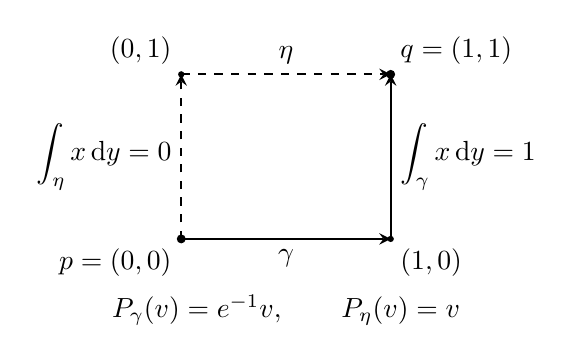
\begin{tikzpicture}[>=stealth,scale=0.95]
		\draw[thick,->] (0,0)--(2.8,0) node[midway,below] {\(\gamma\)};
		\draw[thick,->] (2.8,0)--(2.8,2.2);
		\draw[dashed,thick,->] (0,0)--(0,2.2);
		\draw[dashed,thick,->] (0,2.2)--(2.8,2.2) node[midway,above] {\(\eta\)};
		\fill (0,0) circle (1.7pt) node[below left] {\(p=(0,0)\)};
		\fill (2.8,2.2) circle (1.7pt) node[above right] {\(q=(1,1)\)};
		\fill (2.8,0) circle (1.2pt) node[below right] {\((1,0)\)};
		\fill (0,2.2) circle (1.2pt) node[above left] {\((0,1)\)};
		\node[left] at (0,1.1) {\(\displaystyle\int_\eta x\,\mathrm{d}y=0\)};
		\node[right] at (2.8,1.1) {\(\displaystyle\int_\gamma x\,\mathrm{d}y=1\)};
		\node at (1.4,-0.95) {\(P_\gamma(v)=e^{-1}v,\qquad P_\eta(v)=v\)};
	\end{tikzpicture}
	\caption{同一个联络 \(\alpha=x\,\mathrm{d}y\) 沿两条路径比较相同的两个纤维，得到不同线性同构。实线路径先水平后竖直，虚线路径的顺序相反。}
	\label{g1:fig:path-transport}
\end{figure}

\end{example}

\subsection{由平行移动恢复联络}
\label{g1:subsec:1502:03}

给定局部截面 \(S\)，式 \(S(\gamma(t))-S(\gamma(0))\) 一般没有意义，因为两个向量不在同一纤维。先用反向运输 \(P_{\gamma,0\leftarrow t}\) 把第一个向量送回起点，就能在固定向量空间中取差商。这个操作说明平行移动保存了联络的全部一阶信息。

\begin{theorem}[由运输恢复联络]\label{g1:thm:connection-from-transport}
	设 \(E\to M\) 为实有限秩光滑向量丛，\(M\) 可带边界，\(\nabla\) 为给定联络，\(P\) 是由该联络构造的平行移动。对光滑曲线 \(\gamma:I\to M\)、任意沿曲线的光滑截面 \(s\) 与固定 \(t_0\in I\)，在固定纤维 \(E_{\gamma(t_0)}\) 中有
	\begin{equation}\label{g1:eq:transported-section-derivative}
		\frac{\mathrm{d}}{\mathrm{d}t}\bigl(P_{\gamma,t_0\leftarrow t}s(t)\bigr)
		=P_{\gamma,t_0\leftarrow t}\mathrm{D}_t s.
	\end{equation}
	特别地，若 \(\gamma(0)=p\)、\(\gamma'(0)=v\)，\(S\) 是 \(p\) 附近的光滑截面，则
	\begin{equation}\label{g1:eq:connection-recovery-limit}
		(\nabla_vS)_p
		=\lim_{t\to0}\frac{P_{\gamma,0\leftarrow t}S(\gamma(t))-S(p)}{t}.
	\end{equation}
	若曲线只在零点的一侧有定义，则使用相应的单侧极限。因此同一向量丛上，若两个光滑联络沿所有分片光滑路径产生相同的平行移动，则两个联络相同。
\end{theorem}
\begin{proof}
	先在包含所考察时刻的一个标架域内计算。设从该局部初始时刻到 \(t\) 的平行移动矩阵为 \(U(t)\)，则 \(U'=-BU\)，且 \(U\) 可逆。对 \(U^{-1}U=I\) 求导，得到
	\[
		(U^{-1})'=-U^{-1}U'U^{-1}=U^{-1}B.
	\]
	若 \(s(t)=e(\gamma(t))u(t)\)，则把它运回局部初始纤维后的分量为 \(U(t)^{-1}u(t)\)，而
	\[
		\frac{\mathrm{d}}{\mathrm{d}t}(U^{-1}u)=U^{-1}(u'+Bu).
	\]
	右端恰是 \(\mathrm{D}_ts\) 反向运输后的分量。若固定的 \(t_0\) 不在这一标架域内，先运回局部初始时刻，再接上从该时刻到 \(t_0\) 的固定线性映射；固定线性映射与求导相容，故\eqref{g1:eq:transported-section-derivative}仍成立。

	现在取 \(s=S\circ\gamma\)、\(t_0=0\)，在零点求导。由 \(P_{\gamma,0\leftarrow0}=\operatorname{id}\) 及沿曲线导数与 \(\nabla_{\gamma'}S\) 的相容关系，得到\eqref{g1:eq:connection-recovery-limit}。同一局部计算也证明单侧极限的版本。

	在内部点，每个 \(v\in \mathrm{T}_pM\) 都能由坐标直线给出一条双侧小曲线的初速度，故相同的运输决定所有 \(\nabla_vS\)。在边界点取 \(x^n\ge0\)、\(x(p)=0\) 的图。若 \(v^n\ge0\)，坐标曲线 \(t\mapsto tv\)、\(t\ge0\)，留在半空间中，单侧公式决定 \(\nabla_vS\)。若 \(v^n<0\)，则 \(-v\) 是向内方向，用已经得到的值及 \(\nabla_vS=-\nabla_{-v}S\) 决定它。故两个给定联络若有相同运输，在边界点也相同。零维底流形没有非零切向方向，唯一性同样成立。
\end{proof}

边界处需要保留上述区别。一条以边界点为内部参数时刻、始终留在半空间中的双侧曲线，其法向坐标在该时刻取得局部最小值，所以法向速度必为零。不能用这种曲线代表所有切向量；向内方向由单侧曲线实现，向外方向再通过联络关于方向的线性性决定。

\ProseParagraphBreak

定理恢复的是一个已经给定的联络所产生的运输。若只向每条路径任意指定一个线性同构，即使其中部分映射满足拼接规律，也还不能直接把差商宣布为联络：差商的存在、对路径一阶信息的依赖及所需光滑性都要另外验证。本节得到的是联络与其运输之间的确定关系和唯一性。

\subsection{度量联络和长度保持}
\label{g1:subsec:1502:04}

丛度量 \(g\) 为每个纤维提供内积，存在性已由\cref{g1:thm:bundle-metric-existence}证明。但任意联络不一定在运输时保长；前面 \(x\,\mathrm{d}y\) 的例子，在标准纤维内积下就可能缩短向量。要求“沿途不变的向量保持内积”，应当对应一条关于 \(g\) 与 \(\nabla\) 的微分条件。

\begin{definition}[度量联络]\label{g1:def:metric-connection}
	设 \(E\to M\) 为实有限秩光滑向量丛，\(g\) 是光滑正定丛度量。若联络 \(\nabla\) 对所有局部向量场 \(X\) 和局部截面 \(S,T\) 满足
	\[
		X\bigl(g(S,T)\bigr)=g(\nabla_XS,T)+g(S,\nabla_XT),
	\]
	则称其为关于 \(g\) 的\term[dulianglianluo]{度量联络}[metric connection]，也称与 \(g\) 相容。这就是诱导张量联络下的 \(\nabla g=0\)。
\end{definition}

\begin{proposition}[度量相容与平行移动]\label{g1:prop:metric-parallel-transport}
	设 \(M\) 为有限维光滑流形，允许有边界，\(E\to M\) 为实有限秩光滑向量丛，带光滑正定度量 \(g\) 和联络 \(\nabla\)。以下条件等价：
	\begin{enumerate}
		\item \(\nabla g=0\)。
		\item 在每个局部标架 \(e\) 中，令 \(G=(g(e_i,e_j))\)、\(\nabla e=eA\)，则
		\begin{equation}\label{g1:eq:metric-connection-matrix}
			\mathrm{d}G=A^{\mathsf T}G+GA.
		\end{equation}
		\item 对每条光滑曲线及任意两个沿曲线的光滑截面 \(s,t\)，有
		\[
			\frac{\mathrm{d}}{\mathrm{d}\tau}g(s(\tau),t(\tau))
			=g(\mathrm{D}_\tau s,t)+g(s,\mathrm{D}_\tau t).
		\]
		\item 每条有限分片光滑路径的平行移动都是端点纤维之间的内积等距同构。
	\end{enumerate}
	因而也可以把最后一项等价地写为所有平行移动保持每个向量的长度。
\end{proposition}
\begin{proof}
	将度量相容条件应用于局部基截面 \(e_i,e_j\)。\(\nabla e_j=\sum_k e_kA^k{}_j\)，所以右边的两个矩阵分别为 \(A^{\mathsf T}G\) 和 \(GA\)，得到第二项。反过来，把任意截面写成 \(eu,ev\)，对 \(u^{\mathsf T}Gv\) 使用乘积法则，第二项就给出第一项。

	沿曲线记 \(B=A(\gamma')\)。第二项拉回曲线成为 \(G'=B^{\mathsf T}G+GB\)。于是
	\[
		\frac{\mathrm{d}}{\mathrm{d}\tau}(u^{\mathsf T}Gv)
		=(u'+Bu)^{\mathsf T}Gv+u^{\mathsf T}G(v'+Bv),
	\]
	恰为第三项。两个截面都平行时，右端为零，故内积沿每个光滑片恒定；连续性使这些常值在分段端点吻合。这证明第四项。

	反过来假设第四项。对 \(p\) 附近的局部截面 \(S,T\) 及过 \(p\) 的曲线，令
	\[
		\widehat S(\tau)=P_{\gamma,0\leftarrow\tau}S(\gamma(\tau)),\qquad
		\widehat T(\tau)=P_{\gamma,0\leftarrow\tau}T(\gamma(\tau)).
	\]
	运输保内积，故 \(g_{\gamma(\tau)}(S,T)=g_p(\widehat S(\tau),\widehat T(\tau))\)。在零点求导，再用\cref{g1:thm:connection-from-transport}，得到方向 \(v=\gamma'(0)\) 上的度量相容等式。内部点可取任意 \(v\)；边界处先取向内的单侧曲线，再利用等式两边关于 \(v\) 的线性性处理向外方向。因此第一项成立。

	最后，保内积必然保长度；反过来，实内积由
	\[
		g(v,w)=\frac12\bigl(|v+w|_g^2-|v|_g^2-|w|_g^2\bigr)
	\]
	恢复。平行移动已经线性，故保全部向量的长度也保证保内积。
\end{proof}

在正交归一标架中 \(G=I_r\)，矩阵条件简化为 \(A^{\mathsf T}+A=0\)，即每个 \(A(X)\) 为斜对称矩阵。在一般标架中却不能直接要求 \(A\) 斜对称，必须保留 \(\mathrm{d}G\) 这一项。度量可能随基点变化，而非正交标架自身的长度也会变化。

\begin{proposition}[度量联络的存在]\label{g1:prop:metric-connection-existence}
	设 \(M\) 为有限维、Hausdorff、第二可数的光滑流形，允许有边界，\(E\to M\) 为实有限秩光滑向量丛，\(g\) 为光滑正定丛度量。则 \(E\) 上存在与 \(g\) 相容的联络。给定一个度量联络后，所有其他度量联络恰为 \(\nabla+K\)，其中 \(K\in\Omega^1(M;\operatorname{End}E)\) 满足每个 \(K(X)\) 关于 \(g\) 斜伴随。
\end{proposition}
\begin{proof}
	由\cref{g1:thm:connection-existence}取任意联络 \(\nabla^0\)，再修正它不保持度量的部分。定义
	\[
		Q_X(S,T)=Xg(S,T)-g(\nabla^0_XS,T)-g(S,\nabla^0_XT).
	\]
	Leibniz 法则使这里对 \(S,T\) 的导数项在乘以函数时抵消，故 \(Q\) 对 \(X,S,T\) 都是逐点线性的；它还是光滑的，且对 \(S,T\) 对称。正定性使每个纤维的 \(g\) 非退化，因此存在唯一的 \(C_X\in\operatorname{End}(E)\)，满足
	\[
		g(C_XS,T)=\frac12Q_X(S,T).
	\]
	在局部标架中，若 \(Q_X\) 的对称矩阵为 \(Q(X)\)，这个算子为 \(C_X=\tfrac12G^{-1}Q(X)\)。矩阵逆光滑，故 \(C\) 是光滑的 \(\operatorname{End}E\) 值一形式。

	由\cref{g1:prop:connection-affine-space}，\(\nabla=\nabla^0+C\) 仍是联络。对称性给出
	\begin{align*}
		(\nabla_Xg)(S,T)&=Q_X(S,T)-g(C_XS,T)-g(S,C_XT)\\
		&=Q_X(S,T)-\tfrac12Q_X(S,T)-\tfrac12Q_X(S,T)=0.
	\end{align*}
	因此修正后的联络与度量相容。在矩阵语言中，这一修正是
	\[
		A=A^0+\frac12G^{-1}\bigl(\mathrm{d}G-(A^0)^{\mathsf T}G-GA^0\bigr).
	\]

	若 \(\widetilde\nabla=\nabla+K\)，其中 \(\nabla\) 已度量相容，则
	\[
		(\widetilde\nabla_Xg)(S,T)=-g(K(X)S,T)-g(S,K(X)T).
	\]
	因而 \(\widetilde\nabla\) 也相容，当且仅当每个 \(K(X)\) 斜伴随。这证明了最后的全部刻画。
\end{proof}

\begin{example}\label{g1:exm:rotating-metric-transport}
	在平凡二维丛中取标准内积，令
	\[
		J=\begin{pmatrix}0&-1\\1&0\end{pmatrix},\qquad A=J\,\alpha
	\]
	其中 \(\alpha\) 是任意实一形式。因为 \(J^{\mathsf T}=-J\)，这是度量联络。沿路径记 \(\theta(t)=\int_{t_0}^t \alpha(\gamma'(v))\,\mathrm{d}v\)，则
	\[
		u(t)=\exp(-\theta(t)J)u_0
		=\begin{pmatrix}\cos\theta(t)&\sin\theta(t)\\-\sin\theta(t)&\cos\theta(t)\end{pmatrix}u_0.
	\]
	矩阵求导给出 \(u'=-J\,\alpha(\gamma')u\)，因此这就是平行解。它保持长度，转角却是 \(-\theta\)，再次显示平行方程中的负号。保长不表示每条环路运输都为恒等；它只把可能的运输限制在纤维的正交变换之中。
\end{example}

% 纲要条目排为编号小节标题，并进入目录与书签；说明段仍保留于纲要注释中。

% !TeX root = ../../Book1.tex
% 纲要标题：### 15.3 曲率与结构方程
% 纲要位置：几何学计划纲要.md，第 708 行。
% 正文状态：初稿；尚未正式审核。

% 纲要内容开始
% 
% * 二阶协变微分及张量性
% * 外协变微分与曲率矩阵
% * 曲率的换标架规律与小环路运输
% * Bianchi 恒等式的结构证明
% 
% 纲要内容结束

\section{曲率与结构方程}
\label{g1:sec:1503}

联络使我们能够沿路径比较纤维中的向量，但两条同起点、同终点的路径未必给出同一种比较。在第九章的曲面例子中，绕小圈后的转角由曲率控制。一般向量丛中的返回变换可以伸缩、剪切，也可以旋转，因而需要一个取值于纤维自同态的对象来记录这种变化。本节把它从二阶协变微分中构造出来，再说明它怎样出现在小环路的运输中。

\ProseParagraphBreak

以下 \(E\to M\) 是有限秩实光滑向量丛，\(M\) 有限维、Hausdorff、第二可数，允许边界，\(\nabla\) 是光滑联络。沿用行标架 \(e\)、列分量 \(u\) 和 \(\nabla s=e(\mathrm{d}u+Au)\) 的约定。外微分及分次乘积法则使用\cref{g1:thm:exterior-derivative}；向量场括号的顺序仍为 \([X,Y]=XY-YX\)。边界处使用局部光滑延拓定义括号；\eqref{g1:eq:lie-bracket-product}中的乘法法则由同一坐标计算继续成立。

\subsection{二阶协变微分及张量性}
\label{g1:subsec:1503:01}

单独的 \(\nabla_X\nabla_Ys\) 会依赖 \(Y\) 及 \(s\) 在邻近点的变化。交换 \(X,Y\) 可以消去一部分二阶项，但若方向场自身不交换，还须减去它们的 Lie 括号所贡献的一阶变化。这正是第八章曲面曲率定义中出现第三项的原因，现在同一构造适用于任意向量丛。

\begin{definition}[丛联络的曲率]\label{g1:def:bundle-curvature}
	设 \(E\to M\) 为实光滑向量丛，\(\nabla\) 为其联络，允许 \(M\) 带边界。定义
	\[
		R^\nabla(X,Y)s=\nabla_X\nabla_Ys-\nabla_Y\nabla_Xs-\nabla_{[X,Y]}s,
		\qquad X,Y\in\mathfrak X(M),\quad s\in\Gamma(E).
	\]
	称 \(R^\nabla\) 为该联络的曲率；不致混淆时记作 \(R\)。
\end{definition}

\begin{proposition}[曲率的张量性]\label{g1:prop:bundle-curvature-tensorial}
	设 \(E\to M\) 为实光滑向量丛，\(M\) 可带边界，\(\nabla\) 为光滑联络。对光滑向量场 \(X,Y\) 和光滑截面 \(s\)，令
	\[
		R(X,Y)s=\nabla_X\nabla_Ys-\nabla_Y\nabla_Xs-\nabla_{[X,Y]}s.
	\]
	此运算对 \(X,Y,s\) 均为 \(C^\infty(M)\) 线性，并对前两个变量反对称。因此它唯一确定一个光滑截面
	\[
		R\in\Omega^2(M;\operatorname{End}E)
		=\Gamma(\Lambda^2\mathrm{T}^*M\otimes\operatorname{End}E).
	\]
	在点 \(p\)，\(R_p(v,w)\) 是 \(E_p\) 上的线性自同态，只依赖 \(v,w\in \mathrm{T}_pM\) 和被作用的纤维向量。
\end{proposition}
\begin{proof}
	实多线性和反对称性由定义得到。对光滑函数 \(f\)，先回忆\eqref{g1:eq:lie-bracket-product}的 \([fX,Y]=f[X,Y]-Y(f)X\)。该等式在边界处仍由局部延拓成立。于是
	\begin{align*}
		R(fX,Y)s
		&=f\nabla_X\nabla_Ys-\nabla_Y(f\nabla_Xs)-\nabla_{f[X,Y]-Y(f)X}s\\
		&=fR(X,Y)s.
	\end{align*}
	两个含 \(Y(f)\nabla_Xs\) 的项相消；第二变量的函数线性再由反对称性得到。

	对截面 \(fs\)，展开
	\[
		\nabla_X\nabla_Y(fs)
		=X(Yf)s+(Yf)\nabla_Xs+(Xf)\nabla_Ys+f\nabla_X\nabla_Ys.
	\]
	交换 \(X,Y\) 后，一阶交叉项抵消。再减去 \(\nabla_{[X,Y]}(fs)\)，额外剩余项为 \((X(Yf)-Y(Xf)-[X,Y]f)s=0\)，故 \(R(X,Y)(fs)=fR(X,Y)s\)。在局部坐标标架和丛标架中展开三个输入，函数线性把所有分量移到外面，点处结果便只依赖这些分量在该点的值。各基向量上的结果光滑，故得到所述光滑丛值二形式。
\end{proof}

这里的“二形式”只计算两个切向输入；它的输出不是实数，而是一个还可以作用于纤维向量的线性映射。若 \(E=\mathrm{T}M\)，这就是\cref{g1:def:surface-curvature-tensor}所用曲率的高维版本；若 \(E\) 是一条线丛，则每个纤维自同态只是一个实数倍。

\begin{definition}\label{g1:def:flat-connection}
	若光滑向量丛联络的曲率处处为零，即 \(R^\nabla=0\)，称该联络为\term[pingtanlianluo]{平坦联络}[flat connection]。这个条件针对给定联络；说一个丛具有平坦联络，还须指定或证明这样的联络存在。
\end{definition}

平坦的定义目前只表达一个局部微分条件。它是否足以得到平行标架，以及是否使所有同端点路径的运输相同，需要\secref{g1:sec:1505}的构造来回答。

\subsection{外协变微分与曲率矩阵}
\label{g1:subsec:1503:02}

普通外微分作用于实值形式，联络作用于丛截面。要把它们组织成同一个运算，回顾\cref{g1:def:bundle-valued-form}的记号
\[
	\Omega^k(M;E)=\Gamma(\Lambda^k\mathrm{T}^*M\otimes E).
\]
其元素在一点接受 \(k\) 个切向量，交替多线性地输出一个纤维向量。在标架 \(e\) 中写为 \(\eta=\sum_a\eta^a\otimes e_a\)，其中 \(\eta^a\) 是普通 \(k\) 形式；简记成 \(e\eta_e\)，\(\eta_e=(\eta^a)\) 为列。换标架 \(e'=eg\) 时，列分量变为 \(\eta_{e'}=g^{-1}\eta_e\)。

\ProseParagraphBreak

矩阵值形式相乘时，同时作矩阵乘法和形式楔积。若 \(B\) 是矩阵值 \(p\) 形式、\(C\) 是矩阵值 \(q\) 形式，规定
\[
	(B\wedge C)^a{}_b=\sum_c B^a{}_c\wedge C^c{}_b.
\]
它结合，但一般不满足普通标量形式的分次交换律。特别地，\(A\wedge A\) 未必为零，因为不同矩阵系数未必交换。矩阵乘列形式也按同样规则定义。

\begin{proposition}[外协变微分]\label{g1:prop:exterior-covariant-derivative}
	设 \(\nabla\) 为实光滑向量丛 \(E\to M\) 上的联络。存在唯一的实线性局部算子
	\[
		\mathrm{d}_\nabla:\Omega^k(M;E)\longrightarrow\Omega^{k+1}(M;E)
	\]
	在零次截面上等于 \(\nabla\)，并满足对标量 \(p\) 形式 \(\alpha\) 与丛值形式 \(\eta\)，
	\[
		\mathrm{d}_\nabla(\alpha\wedge\eta)
		=\mathrm{d}\alpha\wedge\eta+(-1)^p\alpha\wedge\mathrm{d}_\nabla\eta.
	\]
	在联络矩阵为 \(A\) 的标架中，它由
	\begin{equation}\label{g1:eq:exterior-covariant-local}
		\mathrm{d}_\nabla(e\eta_e)=e(\mathrm{d}\eta_e+A\wedge\eta_e)
	\end{equation}
	给出，称为\term[waixiebianweifen]{外协变微分}[exterior covariant derivative]。
\end{proposition}
\begin{proof}
	先按局部公式定义。令 \(e'=eg\)，则\eqref{g1:eq:connection-frame-change}给出 \(A'=g^{-1}Ag+g^{-1}\mathrm{d}g\)，而微分 \(g^{-1}g=I\) 得
	\[
		\mathrm{d}(g^{-1})=-g^{-1}(\mathrm{d}g)g^{-1}.
	\]
	于是
	\begin{align*}
		\mathrm{d}(g^{-1}\eta_e)+A'\wedge(g^{-1}\eta_e)
		&=-g^{-1}(\mathrm{d}g)g^{-1}\wedge\eta_e+g^{-1}\mathrm{d}\eta_e\\
		&\quad+g^{-1}A\wedge\eta_e+g^{-1}(\mathrm{d}g)g^{-1}\wedge\eta_e\\
		&=g^{-1}(\mathrm{d}\eta_e+A\wedge\eta_e).
	\end{align*}
	结果按丛值形式的分量变换，因而粘成整体算子。它在零次时就是联络，分次乘积法则则由普通外微分的规则及 \(A\wedge\alpha=(-1)^p\alpha\wedge A\) 得到；这里 \(\alpha\) 是标量，允许这样换序。

	反过来，任意局部丛值形式都是 \(\sum_a\eta^a\otimes e_a\)。对每项使用规定的乘积法则，结果只能为 \(\mathrm{d}\eta^a\otimes e_a+(-1)^k\eta^a\wedge\nabla e_a\)，移过一次形式后正是\eqref{g1:eq:exterior-covariant-local}，所以唯一。
\end{proof}

后文有时将 \(\mathrm{d}_\nabla\) 简记为 \(\mathrm{D}\)，将自同态丛诱导联络的外协变微分简记为 \(\mathrm{D}_{\operatorname{End}}\)。普通外微分平方为零，外协变微分却不一定如此。差别正好是曲率。

\begin{theorem}[曲率的结构方程]\label{g1:thm:curvature-structure-equation}
	设 \(\nabla\) 为实光滑向量丛 \(E\to M\) 上的联络，\(A\) 是某局部标架中的联络矩阵。曲率 \(R\) 在该标架中的矩阵值二形式为
	\begin{equation}\label{g1:eq:curvature-matrix}
		F=\mathrm{d}A+A\wedge A.
	\end{equation}
	对每个 \(\eta\in\Omega^k(M;E)\)，有 \(\mathrm{d}_\nabla^2\eta=R\wedge\eta\)，局部分量即 \(F\wedge\eta_e\)。
\end{theorem}
\begin{proof}
	由局部公式及 \(\mathrm{d}^2=0\)，逐项计算
	\begin{align*}
		(\mathrm{d}+A\wedge)^2\eta_e
		&=\mathrm{d}A\wedge\eta_e-A\wedge\mathrm{d}\eta_e
		+A\wedge\mathrm{d}\eta_e+A\wedge A\wedge\eta_e\\
		&=(\mathrm{d}A+A\wedge A)\wedge\eta_e.
	\end{align*}
	还须确认这确实是先前定义的曲率。对零次截面 \(s=e u\)，把两次协变导数展开并扣除括号项，导数作用于 \(u\) 的项抵消，余下
	\[
		e^{-1}R(X,Y)s
		=\bigl(X(A(Y))-Y(A(X))-A([X,Y])
		+A(X)A(Y)-A(Y)A(X)\bigr)u.
	\]
	由\eqref{g1:eq:exterior-one-form-evaluation}，前三项是 \(\mathrm{d}A(X,Y)\)，后两项是 \((A\wedge A)(X,Y)\)，故所列 \(F\) 表示 \(R\)。一般次数的结论随第一段计算得到。
\end{proof}

在坐标 \(x^i\) 中写 \(A=\sum_i A_i\,\mathrm{d}x^i\)，则
\[
	F=\sum_{i<j}F_{ij}\,\mathrm{d}x^i\wedge\mathrm{d}x^j,
	\qquad F_{ij}=\partial_iA_j-\partial_jA_i+[A_i,A_j].
\]
这里对 \(i<j\) 求和，没有额外的 \(1/2\)。最后一项是矩阵交换子，它记录纤维方向的两次线性变化不交换，不能用标量一形式自楔为零的规则删掉。

\begin{example}[常系数也可能有曲率]\label{g1:exm:constant-noncommuting-connection}
	在 \(\mathbb R^2\times\mathbb R^2\) 的标准标架中取
	\[
		A=B\,\mathrm{d}x+C\,\mathrm{d}y,\qquad
		B=\begin{pmatrix}0&1\\0&0\end{pmatrix},\quad
		C=\begin{pmatrix}0&0\\1&0\end{pmatrix}.
	\]
	虽然 \(\mathrm{d}A=0\)，但
	\[
		F=[B,C]\,\mathrm{d}x\wedge\mathrm{d}y
		=\begin{pmatrix}1&0\\0&-1\end{pmatrix}\mathrm{d}x\wedge\mathrm{d}y\ne0.
	\]
	因此系数恒定、底空间单连通，都不能替代曲率为零。沿一条路径的方程只涉及一个时间变量；同时要求两个方向上的运输相容，才会发现这里的交换子。
\end{example}

在线丛的局部标架中，\(A\) 是标量一形式，\(A\wedge A=0\)，所以 \(F=\mathrm{d}A\)。在第九章的正向正交曲面标架中，\eqref{g1:eq:surface-frame-connection}给出
\[
	A=\begin{pmatrix}0&-\omega\\\omega&0\end{pmatrix},\qquad
	F=\begin{pmatrix}0&-\mathrm{d}\omega\\\mathrm{d}\omega&0\end{pmatrix}.
\]
该例中 \(A\wedge A=0\)，并由\eqref{g1:eq:surface-curvature-form}得到 \(\mathrm{d}\omega=-K\,\mathrm{d}A\)。这里最后的 \(\mathrm{d}A\) 沿用曲面面积形式的记号，与前面“对矩阵 \(A\) 求外微分”的 \(\mathrm{d}A\) 对象不同；在一般丛公式中，\(A\) 始终表示联络矩阵。

\subsection{曲率的换标架规律与小环路运输}
\label{g1:subsec:1503:03}

联络矩阵的变换律含有 \(\mathrm{d}g\)，说明它不按张量变换。曲率已经证明是张量，因而应当只发生纤维基变换，不再出现新的导数项。

\begin{proposition}[曲率的换标架公式]\label{g1:prop:curvature-frame-change}
	若同一实向量丛联络在标架 \(e\) 与 \(e'=eg\) 中的曲率矩阵分别为 \(F,F'\)，则
	\[
		F'=g^{-1}Fg.
	\]
	因此曲率是否为零与标架无关；对固定的切向输入，所得自同态的迹、行列式等共轭不变量也与标架无关。
\end{proposition}
\begin{proof}
	对任意列向量 \(u'\)，同一截面为 \(s=e'u'=e(gu')\)。曲率的纤维线性给出 \(R(X,Y)s=eF(X,Y)g u'\)，另一方面它等于 \(e'F'(X,Y)u'=egF'(X,Y)u'\)。因此 \(Fg=gF'\)，得到结论。这个证明也说明变换律中没有导数项的原因：\(R\) 对截面是逐点线性的。
\end{proof}

\begin{proposition}[小方环的运输]\label{g1:prop:small-loop-curvature}
	设 \(p\) 是光滑流形 \(M\) 的内点，\(\dim M\geq2\)，\(E\to M\) 为秩 \(r\) 实光滑向量丛，\(\nabla\) 为其光滑联络。取以 \(p\) 为原点的坐标及丛标架，记联络矩阵为 \(A\)，曲率矩阵为 \(F=\mathrm{d}A+A\wedge A=\sum_{i<j}F_{ij}\,\mathrm{d}x^i\wedge\mathrm{d}x^j\)。令 \(\gamma_\varepsilon\) 依次沿坐标方形的 \(+x^1,+x^2,-x^1,-x^2\) 四边行进，每边坐标长度为 \(\varepsilon>0\)，其余坐标为零。则在 \(E_p\) 的该标架中，
	\begin{equation}\label{g1:eq:small-loop-curvature}
		P_{\gamma_\varepsilon}
		=I-\varepsilon^2F_{12}(p)+O(\varepsilon^3).
	\end{equation}
	余项指选定矩阵范数下存在与充分小 \(\varepsilon\) 无关的常数 \(C\)，使其范数不超过 \(C\varepsilon^3\)。
\end{proposition}
\begin{proof}
	先用换标架消去一点处的联络系数。令 \(g(x)=I-\sum_i x^iA_i(p)\)，缩小邻域可使 \(g\) 可逆。由变换律，\(g(p)=I\) 且 \(A'_i(p)=A_i(p)+\partial_i g(p)=0\)。新旧标架在基点相同，故返回映射的基点矩阵不变，曲率矩阵在基点也不变。以下在这组新标架中计算并省去撇号。

	四边上 \(A_i=O(\varepsilon)\)。把一条边用坐标长度参数化，平行移动的矩阵满足 \(U'=-B(t)U\)、\(U(0)=I\)，其中时间长度为 \(\varepsilon\)、\(\|B\|\leq C\varepsilon\)。积分方程及\cref{g1:lem:gronwall-estimate}给出 \(\|U\|\leq e^{C\varepsilon^2}\) 和 \(U-I=O(\varepsilon^2)\)，于是再次代回积分方程得
	\[
		U=I-\int_{\text{该边}}A+O(\varepsilon^4).
	\]
	把四段按实际行进顺序相乘，两个积分项的乘积也是 \(O(\varepsilon^4)\)，所以
	\[
		P_{\gamma_\varepsilon}=I-\oint_{\gamma_\varepsilon}A+O(\varepsilon^4).
	\]
	对每个矩阵条目用\cref{g1:thm:stokes-corners}的矩形情形，按\eqref{g1:eq:rectangle-boundary-signs}取正向边界，再对系数作 Taylor 展开，有
	\[
		\oint_{\gamma_\varepsilon}A
		=\int_0^\varepsilon\int_0^\varepsilon
		(\partial_1A_2-\partial_2A_1)(s,t,0,\ldots,0)\,\mathrm{d}s\,\mathrm{d}t
		=\varepsilon^2F_{12}(p)+O(\varepsilon^3).
	\]
	最后一步使用光滑性和 \(A(p)=0\)，此时基点的交换子项为零。结合两式得到结论。矩形缩在内点坐标域内，故没有额外的边界条件。
\end{proof}

% !TeX root = ../Book1.tex
% 两条同端点路径及其组成的小正向回路。
\begin{figure}[htbp]
	\centering
	\begin{tikzpicture}[font=\small,scale=1.1]
		\fill[GeometryBlueLight] (0,0) rectangle (3,2.1);
		\draw[->,GeometryGray] (-0.4,0)--(3.8,0) node[right] {\(x^1\)};
		\draw[->,GeometryGray] (0,-0.4)--(0,2.8) node[above] {\(x^2\)};
		\draw[GeometryBlue,very thick,->] (0,0)--(1.7,0);
		\draw[GeometryBlue,very thick] (1.7,0)--(3,0);
		\draw[GeometryBlue,very thick,->] (3,0)--(3,1.3);
		\draw[GeometryBlue,very thick] (3,1.3)--(3,2.1);
		\draw[orange!80!black,very thick,->] (0,0)--(0,1.3);
		\draw[orange!80!black,very thick] (0,1.3)--(0,2.1);
		\draw[orange!80!black,very thick,->] (0,2.1)--(1.7,2.1);
		\draw[orange!80!black,very thick] (1.7,2.1)--(3,2.1);
		\fill (0,0) circle[radius=1.8pt] node[below left] {\(p\)};
		\fill (3,2.1) circle[radius=1.8pt] node[above right] {\(q\)};
		\node[below] at (3,0) {\(\varepsilon\)};
		\node[left] at (0,2.1) {\(\varepsilon\)};
		\node[GeometryBlue] at (2.3,0.35) {\(\alpha\)};
		\node[orange!80!black] at (0.65,1.7) {\(\beta\)};
		\node[align=center] at (1.6,1.0) {先沿 \(\alpha\)，再沿 \(\beta^{-1}\)\\\(P_{\beta}^{-1}P_{\alpha}\)};
	\end{tikzpicture}
	\caption{两条路径都从 \(p\) 到 \(q\)。用 \(\beta\) 的逆向运输把 \(\alpha\) 的结果带回 \(E_p\)，得到正向小回路的返回变换。它与恒等变换之差的面积首项为 \(-\varepsilon^2F_{12}(p)\)；两边长度在图中仅作示意。}
	\label{g1:fig:curvature-loop}
\end{figure}


\cref{g1:fig:curvature-loop}中的两条折线路径有相同端点，但沿第一条出发、沿第二条反向返回，会形成这个方环。\eqref{g1:eq:small-loop-curvature}说明它们的差首先在面积阶出现，系数就是曲率。负号来自平行方程 \(u'=-A(\dot\gamma)u\) 和所选绕行方向；换成反向环路便反号。一般矩阵系数不交换，不能把小环路的一阶面积近似误写成任意大环路上的 \(P_\gamma=\exp(-\int F)\)。

\subsection{Bianchi 恒等式的结构证明}
\label{g1:subsec:1503:04}

曲率是联络的二阶变化，它自身并不是任意的矩阵值二形式：结构方程强制它满足一个协变微分恒等式。为了准确写出这个式子，先将\cref{g1:prop:induced-connections}给出的 \(\operatorname{End}E\) 联络延拓到自同态值形式。对矩阵值 \(k\) 形式 \(B\)，其外协变微分为
\begin{equation}\label{g1:eq:endomorphism-exterior-derivative}
	\mathrm{d}_{\nabla^{\operatorname{End}}}B
	=\mathrm{d}B+A\wedge B-(-1)^k B\wedge A.
\end{equation}
这里把整体自同态值形式与其局部矩阵暂用同一字母。对 \(B=\beta C\)，其中 \(\beta\) 为标量 \(k\) 形式、\(C\) 为自同态矩阵函数，先用 \(\nabla^{\operatorname{End}}C=\mathrm{d}C+AC-CA\)，再用外协变微分的分次乘积法则，就得到该式；一般 \(B\) 是这类项之和。因而它来自已定义的诱导联络，而不是任意补入的修正项。

下面的\term[bianchihengdengshi]{Bianchi 恒等式}[Bianchi identity]\footnote{Bianchi，Luigi Bianchi（1856--1928），意大利数学家，研究曲面、Riemann 几何及连续变换群。}表达曲率的这种相容性。

\begin{theorem}[Bianchi 恒等式]\label{g1:thm:bianchi-identity}
	设 \(E\to M\) 为实光滑向量丛，\(\nabla\) 为光滑联络，\(R\) 为其曲率，\(\nabla^{\operatorname{End}}\) 为在 \(\operatorname{End}E\) 上诱导的联络。在任一光滑局部标架中，记 \(A,F\) 分别为联络及曲率的矩阵形式。则
	\[
		\mathrm{d}_{\nabla^{\operatorname{End}}}R=0.
	\]
	局部矩阵形式为
	\begin{equation}\label{g1:eq:bianchi-matrix}
		\mathrm{d}F+A\wedge F-F\wedge A=0.
	\end{equation}
\end{theorem}
\begin{proof}
	代入结构方程 \(F=\mathrm{d}A+A\wedge A\)。由于 \(A\) 是一次形式，
	\[
		\mathrm{d}F=\mathrm{d}A\wedge A-A\wedge\mathrm{d}A.
	\]
	另外
	\[
		A\wedge F-F\wedge A
		=A\wedge\mathrm{d}A+A\wedge A\wedge A
		-\mathrm{d}A\wedge A-A\wedge A\wedge A.
	\]
	两式相加，各项成对抵消。上述局部表达是整体 \(\operatorname{End}E\) 联络的外协变微分，所以每张图中为零就意味着整体为零。整个论证只用外微分平方为零、分次乘积法则及矩阵乘法结合性，不要求度量或无挠条件。
\end{proof}

这个恒等式通常称为第二 Bianchi 恒等式；切丛上另有涉及挠率的第一 Bianchi 恒等式，将在下一节得到。

\ProseParagraphBreak

在坐标向量场上，它的可计算形式是
\[
	\partial_iF_{jk}+\partial_jF_{ki}+\partial_kF_{ij}
	+[A_i,F_{jk}]+[A_j,F_{ki}]+[A_k,F_{ij}]=0.
\]
因此一般不能删掉交换子而断言 \(\mathrm{d}F=0\)。在线丛上矩阵系数交换，式子才退化为普通的 \(\mathrm{d}F=0\)。在二维底流形上，恒等式因三形式为零而自动成立；它既不迫使二维曲率为零，也不说明联络可以取成零矩阵。

% 纲要条目排为编号小节标题，并进入目录与书签；说明段仍保留于纲要注释中。

% !TeX root = ../../Book1.tex
% 纲要标题：### 15.4 切丛联络与挠率
% 纲要位置：几何学计划纲要.md，第 715 行。
% 正文状态：初稿；尚未正式审核。

% 纲要内容开始
% 
% * 挠率的坐标无关定义
% * 无挠性和坐标标架
% * 第一结构方程
% * 切丛与一般向量丛的区别
% 
% 纲要内容结束

\section{切丛联络与挠率}
\label{g1:sec:1504}

一般向量丛的联络接受一个切向量方向和一个丛截面，输出同一丛的截面。对切丛，方向场和被微分的截面恰好都是向量场，因而可以交换二者，还可以把结果与 Lie 括号比较。这种额外的比较产生挠率。曲率考察同一向量连续经过两次协变微分后的差别；挠率则从一次协变微分出发，比较方向与被微分向量的交换。

\ProseParagraphBreak

本节 \(\nabla\) 是 \(\mathrm{T}M\) 上的光滑联络，\(M\) 有限维、Hausdorff、第二可数，允许边界。涉及坐标向量场的局部可实现性时，将明确限制在内点。度量不是挠率定义所需的数据，以下也不默认联络保持任何度量。

\subsection{挠率的坐标无关定义}
\label{g1:subsec:1504:01}

在 Euclid 空间的通常导数下，\(\partial_XY-\partial_YX=[X,Y]\)。因此，直接把 \(\nabla_XY-\nabla_YX\) 当成偏离 Euclid 情形的量并不合适：即使使用通常导数，只要所选方向场不交换，它也可能不为零。应当先减去由方向场本身造成的 Lie 括号。

\begin{definition}[挠率]\label{g1:def:torsion}
	切丛联络 \(\nabla\) 的\term[naolv]{挠率}[torsion]定义为
	\begin{equation}\label{g1:eq:torsion-definition}
		T^\nabla(X,Y)=\nabla_XY-\nabla_YX-[X,Y].
	\end{equation}
	若 \(T^\nabla=0\)，称 \(\nabla\) 为\term[wunaolianluo]{无挠联络}[torsion-free connection]。下文不致混淆时简记为 \(T\)。
\end{definition}

第七章也用“挠率”表示空间曲线的标量 \(\tau\)，它描述 Frenet 标架的转动。这里的 \(T\) 是切丛联络的二输入张量，二者的定义和所需数据不同，不能因中文名称相同便代入同一个公式。

\begin{proposition}[挠率的张量性]\label{g1:prop:torsion-tensorial}
	设 \(M\) 为可带边界的光滑流形，\(\nabla\) 为 \(\mathrm{T}M\) 上的光滑线性联络，\(T\) 为其挠率。则 \(T\) 是一个光滑的切丛值二形式，即 \(T\in\Omega^2(M;\mathrm{T}M)\)。在任意局部标架 \((e_i)\) 中，若
	\[
		\nabla_{e_i}e_j=\sum_k\Gamma^k_{ij}e_k,\qquad
		[e_i,e_j]=\sum_k c^k_{ij}e_k,
	\]
	则
	\begin{equation}\label{g1:eq:torsion-frame-components}
		T(e_i,e_j)=\sum_k\bigl(\Gamma^k_{ij}-\Gamma^k_{ji}-c^k_{ij}\bigr)e_k.
	\end{equation}
\end{proposition}
\begin{proof}
	由定义，\(T\) 实双线性且反对称。用\eqref{g1:eq:lie-bracket-product}中的 \([fX,Y]=f[X,Y]-Y(f)X\)，得到
	\begin{align*}
		T(fX,Y)
		&=f\nabla_XY-\nabla_Y(fX)-[fX,Y]\\
		&=f\nabla_XY-Y(f)X-f\nabla_YX-f[X,Y]+Y(f)X\\
		&=fT(X,Y).
	\end{align*}
	反对称性随后给出第二个输入的函数线性。因此在局部标架中展开 \(X,Y\)，结果只依赖它们在求值点的分量；各分量又光滑，故为光滑张量。把两个输入取成 \(e_i,e_j\)，直接代入定义便得分量公式。边界处同样的局部延拓计算成立。
\end{proof}

在\secref{g1:sec:0803}中，曲面的诱导联络已经满足 \(\nabla_XY-\nabla_YX=[X,Y]\)，见\cref{g1:prop:surface-connection-properties}。现在可以把该性质简洁地表述为“曲面的诱导联络无挠”。这不是所有切丛联络自动具有的性质。

\subsection{无挠性和坐标标架}
\label{g1:subsec:1504:02}

坐标标架满足 \([\partial_i,\partial_j]=0\)，所以\eqref{g1:eq:torsion-frame-components}化为
\[
	T(\partial_i,\partial_j)=\sum_k(\Gamma^k_{ij}-\Gamma^k_{ji})\partial_k.
\]
于是无挠性等价于每个坐标图中 \(\Gamma^k_{ij}=\Gamma^k_{ji}\)。这里两个下指标分别表示微分方向和被微分向量；只有在坐标标架中，才能不加修正地使用这条对称性判据。一般标架中的正确判据是 \(\Gamma^k_{ij}-\Gamma^k_{ji}=c^k_{ij}\)。

\begin{proposition}[无挠联络的存在与差]\label{g1:prop:torsion-free-affine-space}
	设 \(M\) 为有限维、Hausdorff、第二可数的光滑流形，允许有边界。则 \(\mathrm{T}M\) 上存在无挠光滑联络。对任意两个光滑切丛联络 \(\nabla,\nabla'\)，若 \(\nabla' =\nabla+B\)，其中 \(B\in\Omega^1(M;\operatorname{End}(\mathrm{T}M))\)，则
	\begin{equation}\label{g1:eq:torsion-difference}
		T^{\nabla'}(X,Y)=T^\nabla(X,Y)+B(X)Y-B(Y)X.
	\end{equation}
	无挠联络组成一个仿射空间，其平移向量空间为 \(\Gamma(\operatorname{Sym}^2\mathrm{T}^*M\otimes \mathrm{T}M)\)。
\end{proposition}
\begin{proof}
	将 \(\nabla'\) 代入挠率定义，Lie 括号项相消，就得到差公式。由\cref{g1:thm:connection-existence}，先任选一个切丛联络 \(\nabla\)。其挠率已经证明为张量，所以
	\[
		\nabla^0_XY=\nabla_XY-\tfrac12T^\nabla(X,Y)
	\]
	仍满足联络的两条函数乘法规则。利用 \(T^\nabla(Y,X)=-T^\nabla(X,Y)\)，差公式给出 \(T^{\nabla^0}=T^\nabla-\tfrac12T^\nabla-\tfrac12T^\nabla=0\)。若 \(\nabla\) 已无挠，则 \(\nabla+B\) 无挠当且仅当 \(B(X)Y=B(Y)X\)，这正是 \(\mathrm{T}M\) 值二阶协变张量的对称性。联络之差的唯一性和仿射性质已由\cref{g1:prop:connection-affine-space}给出，限制到该对称子空间即得结论。
\end{proof}

这个构造只解决无挠性。即使原联络保持某个度量，减去一半挠率后也未必继续保持它；章末习题将给出直接计算。我们应当把无挠性、度量相容性和平坦性分别检查。

\begin{example}\label{g1:exm:torsion-free-curved}
	在 \(\mathbb R^2\) 的坐标标架 \((\partial_x,\partial_y)\) 中规定
	\[
		\nabla_{\partial_y}\partial_y=x\partial_x,
		\qquad\nabla_{\partial_x}\partial_x
		=\nabla_{\partial_x}\partial_y
		=\nabla_{\partial_y}\partial_x=0.
	\]
	各 \(\Gamma^k_{ij}\) 对 \(i,j\) 对称，所以 \(T=0\)。然而
	\[
		A=\begin{pmatrix}0&x\,\mathrm{d}y\\0&0\end{pmatrix},\qquad
		F=\mathrm{d}A+A\wedge A=\begin{pmatrix}0&\mathrm{d}x\wedge\mathrm{d}y\\0&0\end{pmatrix}.
	\]
	特别地，\(R(\partial_x,\partial_y)\partial_y=\partial_x\ne0\)。无挠并不保证平坦。
\end{example}

\begin{example}\label{g1:exm:flat-with-torsion}
	仍在 \(\mathbb R^2\)，取处处线性无关的向量场 \(e_1=\partial_x\)、\(e_2=e^x\partial_y\)，规定 \(\nabla_Xe_i=0\) 对所有 \(X\) 成立。对 \(Y=y^1e_1+y^2e_2\)，这具体表示 \(\nabla_XY=X(y^1)e_1+X(y^2)e_2\)，因而确实定义联络。该标架中 \(A=0\)，故 \(F=0\)。但
	\[
		[e_1,e_2]=e_2,\qquad T(e_1,e_2)=-e_2\ne0.
	\]
	若取 \(g=\mathrm{d}x^2+e^{-2x}\mathrm{d}y^2\)，则 \(e_1,e_2\) 为正交规范标架，平行移动保持其分量，因而保持 \(g\)。这同时给出平坦、保持度量而有挠率的联络。
\end{example}

后一个例子还能说明“把联络矩阵变成零”和“找到使所有坐标向量场平行的坐标”不同。它已有整体平行标架，但该标架的 Lie 括号不为零，不能成为坐标标架。

\subsection{第一结构方程}
\label{g1:subsec:1504:03}

设 \(e=(e_1,\ldots,e_n)\) 是切丛局部行标架，\(\theta=(\theta^1,\ldots,\theta^n)^{\mathsf T}\) 是对偶余标架的列，满足 \(\theta^i(e_j)=\delta^i_j\)。这样每个向量场都可写成 \(X=e\theta(X)\)。令 \(\nabla e=eA\)，并将挠率写成 \(T(X,Y)=e\Theta(X,Y)\)，其中 \(\Theta\) 是二形式列。

\begin{proposition}[第一结构方程]\label{g1:prop:first-structure-equation}
	设 \(M\) 为可带边界的光滑 \(n\) 维流形，\(\nabla\) 为其光滑切丛联络，\(T\) 为挠率。在开集 \(U\) 上取光滑行标架 \(e=(e_1,\ldots,e_n)\) 及对偶余标架列 \(\theta\)，令 \(\nabla e=eA\)，并以 \(T(X,Y)=e\Theta(X,Y)\) 定义挠率分量列 \(\Theta\)。则
	\begin{equation}\label{g1:eq:first-structure-equation}
		\Theta=\mathrm{d}\theta+A\wedge\theta.
	\end{equation}
	若 \(g:U\to\operatorname{GL}(n,\mathbb R)\) 光滑，且换标架为 \(e'=eg\)，则 \(\theta'=g^{-1}\theta\)、\(\Theta'=g^{-1}\Theta\)。因而右侧虽由局部形式组成，却表示同一个整体切丛值二形式。
\end{proposition}
\begin{proof}
	联络的局部表达给出
	\[
		\nabla_XY=e\bigl(X(\theta(Y))+A(X)\theta(Y)\bigr).
	\]
	交换 \(X,Y\) 并减去 \([X,Y]=e\theta([X,Y])\)，分量成为
	\[
		X(\theta(Y))-Y(\theta(X))-\theta([X,Y])
		+A(X)\theta(Y)-A(Y)\theta(X).
	\]
	由\eqref{g1:eq:exterior-one-form-evaluation}，前三项正是 \(\mathrm{d}\theta(X,Y)\)；后两项正是 \((A\wedge\theta)(X,Y)\)。这证明第一结构方程。

	由 \(X=e\theta(X)=eg\theta'(X)\) 得 \(\theta'=g^{-1}\theta\)，由 \(T=e\Theta=eg\Theta'\) 得 \(\Theta'=g^{-1}\Theta\)。也可以使用\eqref{g1:eq:connection-frame-change}直接验算：\(\mathrm{d}(g^{-1})\wedge\theta\) 与联络变换中的 \(g^{-1}\mathrm{d}g\wedge g^{-1}\theta\) 恰好抵消，留下 \(g^{-1}(\mathrm{d}\theta+A\wedge\theta)\)。
\end{proof}

现在有两条结构方程：第一条 \(\Theta=\mathrm{d}\theta+A\wedge\theta\) 描述挠率，第二条 \(F=\mathrm{d}A+A\wedge A\) 描述曲率。第一条需要切丛自带的余标架；第二条对任意向量丛成立。在坐标标架中 \(\theta^i=\mathrm{d}x^i\)，所以 \(\mathrm{d}\theta=0\)，无挠性变成 \(A\wedge\theta=0\)。一般标架下不能漏掉 \(\mathrm{d}\theta\)。

\begin{example}\label{g1:exm:polar-torsion-cancellation}
	在极坐标局部区域 \(r>0\) 中，Euclid 平面的正交规范标架为 \(e_1=\partial_r\)、\(e_2=r^{-1}\partial_\varphi\)，其对偶列为 \(\theta=(\mathrm{d}r,r\,\mathrm{d}\varphi)^{\mathsf T}\)。把二者写成笛卡儿分量，\(e_1=(\cos\varphi,\sin\varphi)\)、\(e_2=(-\sin\varphi,\cos\varphi)\)。直接微分得到通常 Euclid 联络的矩阵
	\[
		A=\begin{pmatrix}0&-\mathrm{d}\varphi\\\mathrm{d}\varphi&0\end{pmatrix}.
	\]
	于是
	\[
		\mathrm{d}\theta=\begin{pmatrix}0\\\mathrm{d}r\wedge\mathrm{d}\varphi\end{pmatrix},\qquad
		A\wedge\theta=\begin{pmatrix}0\\-\mathrm{d}r\wedge\mathrm{d}\varphi\end{pmatrix}.
	\]
	两项抵消，\(\Theta=0\)。虽然 \([e_1,e_2]=-r^{-1}e_2\ne0\)，联络仍无挠；标架的不交换性已被 \(\nabla_{e_1}e_2-\nabla_{e_2}e_1\) 准确补偿。这里 \(\mathrm{d}A=0\)、\(A\wedge A=0\)，故曲率也为零。
\end{example}

\begin{proposition}[第一 Bianchi 恒等式]\label{g1:prop:first-bianchi-identity}
	设 \(M\) 为可带边界的光滑流形，\(\nabla\) 为其光滑切丛联络，\(T,R\) 分别为挠率与曲率。任取光滑局部行标架 \(e\) 及对偶余标架列 \(\theta\)，以 \(\nabla e=eA\)、\(T(X,Y)=e\Theta(X,Y)\)、\(R(X,Y)(eu)=eF(X,Y)u\) 定义 \(A,\Theta,F\)。则
	\begin{equation}\label{g1:eq:first-bianchi-identity}
		\mathrm{d}\Theta+A\wedge\Theta=F\wedge\theta.
	\end{equation}
	特别地，若联络无挠，则对任意光滑向量场 \(X,Y,Z\) 有
	\begin{equation}\label{g1:eq:torsion-free-cyclic-curvature}
		R(X,Y)Z+R(Y,Z)X+R(Z,X)Y=0.
	\end{equation}
\end{proposition}
\begin{proof}
	恒等映射 \(\operatorname{Id}_{\mathrm{T}M}\) 可看成一个切丛值一形式，它在 \(X\) 上取值 \(X\)，在标架 \(e\) 中的分量正是 \(\theta\)。第一结构方程说明 \(\mathrm{D}\operatorname{Id}_{\mathrm{T}M}=T\)。对它再作一次外协变微分，\cref{g1:thm:curvature-structure-equation}中的 \(\mathrm{D}^2\eta=F\wedge\eta\) 给出 \(\mathrm{D}T=R\wedge\operatorname{Id}_{\mathrm{T}M}\)，其分量就是\eqref{g1:eq:first-bianchi-identity}。

	若 \(T=0\)，左侧为零。右侧在 \(X,Y,Z\) 上的值为
	\[
		R(X,Y)Z-R(X,Z)Y+R(Y,Z)X.
	\]
	这是二形式与一形式楔积的三个保序项；用 \(R(X,Z)=-R(Z,X)\)，便得到循环恒等式。
\end{proof}

这里的“第一”恒等式把挠率与曲率联系起来；上一节证明的 \(\mathrm{D}_{\operatorname{End}}R=0\) 通常称为第二 Bianchi 恒等式，它对任意向量丛联络成立，并不要求无挠。对有挠率的切丛联络，不能直接套用\eqref{g1:eq:torsion-free-cyclic-curvature}，必须保留\eqref{g1:eq:first-bianchi-identity}的左侧。

\subsection{切丛与一般向量丛的区别}
\label{g1:subsec:1504:04}

挠率构造中的特殊数据，是 \(\mathrm{T}M\) 的纤维正好就是底空间的切向量空间。因此存在无需选择的 \(\mathrm{T}M\) 值一形式 \(X\mapsto X\)，也能对两个切丛截面取 Lie 括号。一般向量丛 \(E\) 的纤维可能是余切空间、张量空间，或者与切向量没有自然关系的向量空间；既没有默认的映射 \(\mathrm{T}M\to E\)，也没有默认的截面 Lie 括号。仅给 \(E\) 一个联络，便没有相应的规范挠率。

\ProseParagraphBreak

如果另行给出 \(E\) 值一形式 \(\eta\)，当然可以构造 \(\mathrm{D}\eta\)。但这是依赖 \(\eta\) 的额外对象，不能只由联络决定。切丛的情形恰好有一个天然选择 \(\eta=\operatorname{Id}_{\mathrm{T}M}\)，才使 \(\mathrm{D}\eta\) 成为联络自身的挠率。

\begin{proposition}[平行标架的坐标实现]\label{g1:prop:parallel-coordinate-frame}
	设 \(M\) 为光滑 \(n\) 维流形，\(U\subseteq\operatorname{Int}M\) 为开集，\(\nabla\) 为 \(\mathrm{T}U\) 上的光滑线性联络，\(e_1,\ldots,e_n\) 是相对于 \(\nabla\) 的光滑平行标架，即 \(\nabla_Xe_i=0\) 对所有向量场 \(X\) 成立。则下列条件等价：联络在 \(U\) 上无挠；\([e_i,e_j]=0\) 对所有 \(i,j\) 成立；每点附近都有坐标 \((y^1,\ldots,y^n)\) 使 \(e_i=\partial/\partial y^i\)。
\end{proposition}
\begin{proof}
	平行性使 \(T(e_i,e_j)=-[e_i,e_j]\)，而挠率是张量，因此前两个条件等价。坐标向量场两两交换，所以第三个条件蕴含第二个。

	现设括号全部为零，取对偶余标架 \(\theta^i\)。由于 \(\theta^i(e_j)=\delta^i_j\) 是常数，外微分的一形式公式给出
	\[
		\mathrm{d}\theta^i(e_j,e_k)=-\theta^i([e_j,e_k])=0.
	\]
	这些向量场张成切空间，故 \(\mathrm{d}\theta^i=0\)。由\cref{g1:cor:local-exactness}，在每个内点的足够小共同邻域上存在光滑函数 \(y^i\)，使 \(\theta^i=\mathrm{d}y^i\)。提醒这里调用的是正次闭形式的局部恰当性，无须这些一形式在整个 \(U\) 上恰当。映射 \(y=(y^1,\ldots,y^n)\) 的微分由余标架组成，处处可逆。\cref{g1:thm:inverse-function}于是给出局部坐标，且 \(\mathrm{d}y^i(e_j)=\delta^i_j\) 强制 \(e_j=\partial/\partial y^j\)。
\end{proof}

下一节将证明，曲率为零恰好允许在足够小的邻域中构造平行标架。与此命题结合，便得到流形内部的结论：平坦且无挠的切丛联络局部可以用联络系数全为零的坐标表示。曲率消失负责产生平行标架，挠率消失负责使这个标架来自坐标。\cref{g1:exm:flat-with-torsion}说明第二步确有独立条件。

\ProseParagraphBreak

边界处须保留区别。闭余标架仍有局部原函数，它们也给出到 Euclid 空间的局部光滑嵌入，但像的边界未必是一个坐标超平面，不能因此断言它们构成标准半空间型边界坐标。例如，Euclid 平面中闭圆盘的通常联络平坦且无挠；若新坐标也使联络系数为零，则逆坐标映射的所有二阶导数都为零，因而它必须局部为仿射映射，而仿射变换不能把圆弧变成直线。因而上面的坐标实现命题特意陈述在内点，边界邻域的平行标架则不受这个限制。

% !TeX root = ../../Book1.tex
% 纲要标题：### 15.5 平坦性、单值与局部实现
% 纲要位置：几何学计划纲要.md，第 722 行。
% 正文状态：初稿；尚未正式审核。

% 纲要内容开始
% 
% * 平坦联络的平行标架构造
% * 单连通区域上的路径无关性
% * 非单连通情形的单值表示
% * 局部曲率与整体平坦丛的区别
% 
% ---
% 
% 纲要内容结束

\section{平坦性、单值与局部实现}
\label{g1:sec:1505}

沿一条给定路径，平行移动总能由常微分方程求出。但如果希望在一个区域内同时比较所有纤维，就要问：改变路径会不会改变比较结果？曲率记录局部绕行造成的差异；当曲率处处为零时，还须判断一条较大的环路能否在区域内收缩。前者是局部微分条件，后者涉及区域的整体拓扑。

\ProseParagraphBreak

本节的底空间是有限维、Hausdorff、第二可数光滑流形，允许有边界，向量丛为有限秩实光滑丛。沿用行标架 \(e=(e_1,\ldots,e_r)\) 与列分量 \(u\) 的约定：
\[
	\nabla(eu)=e(\mathrm{d}u+A u),\qquad
	A'=g^{-1}Ag+g^{-1}\mathrm{d}g,\qquad
	F=\mathrm{d}A+A\wedge A.
\]
其中 \(e'=eg\)。\cref{g1:def:flat-connection}称曲率恒为零的联络为平坦联络；由\cref{g1:eq:curvature-matrix,g1:prop:curvature-frame-change}，这等价于在任意局部标架中 \(F=0\)。下面把这一矩阵条件转成实际可用的标架与运输。

\subsection{平坦联络的平行标架构造}
\label{g1:subsec:1505:01}

若能换到一个联络矩阵为零的标架，平行方程便成为 \(\mathrm{d}u/\mathrm{d}t=0\)：向量沿路径移动时，其分量保持不变。这正是我们希望由 \(F=0\) 得到的局部模型。困难在于同时消去所有坐标方向的联络系数；只沿一条路径求解，并没有完成这件事。

\begin{definition}
	\label{g1:def:parallel-frame}
	设 \(M\) 为可带边界的光滑流形，\(E\to M\) 为实有限秩光滑向量丛，\(\nabla\) 为其光滑联络，\(U\subset M\) 开。若 \(E|_U\) 的光滑局部标架 \(f=(f_1,\ldots,f_r)\) 对每个 \(a\) 都满足 \(\nabla f_a=0\)，则称 \(f\) 为\term[pingxingbiaojia]{平行标架}[parallel frame]。等价地，对任意光滑列函数 \(u\)，有 \(\nabla(fu)=f\,\mathrm{d}u\)。
\end{definition}

\begin{theorem}[平坦局部模型]
	\label{g1:thm:flat-parallel-frame}
	设 \(E\to M\) 是有限秩实光滑向量丛，\(M\) 是有限维、Hausdorff、第二可数光滑流形，允许有边界，\(\nabla\) 是光滑联络。则 \(\nabla\) 平坦当且仅当每点附近存在平行标架。平坦时，给定 \(p\in M\) 及 \(E_p\) 的一个有序基，可以在某个连通邻域 \(U\ni p\) 上选平行标架，使其在 \(p\) 处等于这个基；一旦 \(U\) 固定，这样的平行标架唯一。
\end{theorem}
\begin{proof}
	先从 \(F=0\) 构造标架。秩为零或底空间维数为零时结论直接成立，以下设秩 \(r\geq1\)、维数 \(n\geq1\)。在 \(p\) 附近取坐标及丛标架 \(e\)，使 \(p\) 对应原点，且 \(e(p)\) 等于指定基。缩小后，坐标域可以取为盒
	\[
		B=(-\varepsilon,\varepsilon)^n
		\quad\text{或}\quad
		B=(-\varepsilon,\varepsilon)^{n-1}\times[0,\varepsilon).
	\]
	后一种用于边界点，最后一个坐标是向内的坐标。写 \(A=\sum_{i=1}^n A_i\,\mathrm{d}x^i\)。变换公式说明，把第一个系数变成零，需要解
	\begin{equation}
		\label{g1:eq:flat-first-coordinate-ode}
		\partial_1g(x^1,x')=-A_1(x^1,x')g(x^1,x'),\qquad
		g(0,x')=I_r,
	\end{equation}
	其中 \(x'=(x^2,\ldots,x^n)\) 暂作参数。

	\cref{g1:thm:ode-local-existence-uniqueness,g1:thm:ode-smooth-dependence}给出共同小时间内的解及对 \(x'\) 的光滑依赖，故适当缩小盒后得到光滑矩阵 \(g\)。这里把矩阵的 \(r^2\) 个条目作为普通 Euclid 未知量即可。为核实 \(g\) 始终可逆，同样解 \(\partial_1k=kA_1\)、\(k(0,x')=I_r\)。乘积法则给出 \(\partial_1(kg)=0\)，所以 \(kg=I_r\)，方阵 \(g\) 因而可逆。边界情形中，光滑系数按定义可延拓到半盒周围的开集；在延拓后的开集应用同一个参数定理，再限制回来，便得到光滑到边界的解。最后剩下一维半区间时，只保留从零开始的非负时间。延拓只用于获得解和参数正则性，不要求延拓后的联络仍然平坦。

	在标架 \(e'=eg\) 中记联络矩阵为 \(B=\sum_iB_i\,\mathrm{d}x^i\)。由\eqref{g1:eq:flat-first-coordinate-ode}，\(B_1=0\)。曲率按共轭变换仍为零，而其 \((1,j)\) 分量为
	\[
		0=F'_{1j}
		=\partial_1B_j-\partial_jB_1+B_1B_j-B_jB_1
		=\partial_1B_j,\qquad j\geq2.
	\]
	固定 \(x'\) 后沿第一坐标积分，便得到 \(B_j(x^1,x')=B_j(0,x')\)。因此余下的联络系数实际上只依赖 \(n-1\) 个变量。

	现在对维数归纳。一维时已经全部消去。若 \(n>1\)，截面 \(x^1=0\) 上的矩阵形式 \(\sum_{j=2}^n B_j(0,x')\,\mathrm{d}x^j\) 仍然平坦，因为它的曲率分量就是原来为零的 \(F'_{ij}\)，其中 \(i,j\geq2\)。归纳假设给出 \(h(x')\in\operatorname{GL}(r,\mathbb R)\)，在原点取 \(I_r\)，并消去这个低一维联络的全部系数。让 \(h\) 沿第一坐标方向保持不变，标架 \(f=e' h\) 的第一系数仍为零，其他系数也为零。归纳中的每一步只需缩小坐标盒，并且对半盒采用刚才的延拓与限制方法，所以边界处同样成立。所得 \(f(p)=e(p)\)，完成存在性。

	反过来，若每点附近有平行标架，则其中 \(A=0\)，所以 \(F=\mathrm{d}A+A\wedge A=0\)。曲率是整体定义的张量，局部为零便处处为零。

	最后设 \(f,\widehat f\) 是连通 \(U\) 上的两个平行标架，写 \(\widehat f=f c\)。由 \(\nabla\widehat f=f\,\mathrm{d}c=0\)，得到 \(\mathrm{d}c=0\)。在每个坐标小盒内，沿线段积分各个条目的导数，可知 \(c\) 局部常值；半盒边界也由同一结论或连续性得到。连通性于是使 \(c\) 为一个常矩阵。若两标架在 \(p\) 相同，则 \(c(p)=I_r\)，所以处处相同。
\end{proof}

证明中 \(F_{1j}=0\) 的作用可以具体看见：消去第一方向以后，它保证其余系数不会沿第一方向重新变化。因此逐方向构造可以继续，而不会破坏已经完成的一步。对一般联络，仍能沿第一方向解同一个方程，但剩下的 \(\partial_1B_j\) 可能不为零，归纳便不能如此进行。

\ProseParagraphBreak

若两个平行标架在某个开集上都有定义，换标架公式中的两套联络矩阵都为零，转移矩阵的微分也就为零。因此它在交叠的每个连通分支上恒定，不同分支上可以取不同的常矩阵。这些常矩阵将用于把一条路径上的局部运输接合起来。

\subsection{单连通区域上的路径无关性}
\label{g1:subsec:1505:02}

\cref{g1:thm:parallel-transport}已经给出分片光滑路径上的平行移动。为了用\cref{g1:def:path-homotopy,g1:def:simply-connected}中的连续同伦比较运输，需要先把运输延伸到连续路径。平行标架提供了这个延伸：在每张图中保持分量，再利用交叠处的常转移矩阵接合，路径本身便无须可微。

\begin{lemma}[连续路径上的平坦运输]
	\label{g1:lem:flat-continuous-transport}
	设 \(E\to M\) 是有限秩实光滑向量丛，底流形有限维、Hausdorff、第二可数，允许有边界，\(\nabla\) 平坦。对每条连续路径 \(\gamma:[0,1]\to M\)，可以定义线性同构 \(P_\gamma:E_{\gamma(0)}\to E_{\gamma(1)}\)，使路径位于一个平行标架域内时，运输保持该标架中的分量。此定义与局部标架及细分无关；在分片光滑路径上等于原来的平行移动，并满足下列规律：对另一连续路径 \(\eta:[0,1]\to M\)，当 \(\gamma(1)=\eta(0)\) 时，令 \(\gamma*\eta\) 先走 \(\gamma\) 后走 \(\eta\)；令 \(\bar\gamma(t)=\gamma(1-t)\)，\(e_p(t)=p\) 为常路径。则
	\[
		P_{\gamma*\eta}=P_\eta\circ P_\gamma,\qquad
		P_{\bar\gamma}=P_\gamma^{-1},\qquad
		P_{e_p}=\operatorname{id}_{E_p}.
	\]
	其中 \(p\in M\)。
\end{lemma}
\begin{proof}
	把平行标架 \(f\) 在每点看成同构 \(f(x):\mathbb R^r\to E_x\)。对其定义域 \(U\) 中的两点 \(x,y\)，令
	\[
		T^U_{y\leftarrow x}=f(y)f(x)^{-1}.
	\]
	若 \(\widehat f=fc\) 是另一个平行标架，而 \(x,y\) 位于交叠的同一个连通分支内，则 \(c(y)=c(x)\)，所以两个标架给出的 \(T\) 相同。特别地，若一段连续路径同时落在两个标架域内，其像是连通集，以上比较便适用。

	平行标架域的原像覆盖紧区间。由\cref{g1:lem:lebesgue-number}，存在有限分点 \(0=t_0<\cdots<t_N=1\)，使每段 \(\gamma([t_{j-1},t_j])\) 都落在某个标架域 \(U_j\)。定义
	\[
		P_\gamma
		=T^{U_N}_{\gamma(t_N)\leftarrow\gamma(t_{N-1})}\circ\cdots\circ
		T^{U_1}_{\gamma(t_1)\leftarrow\gamma(t_0)}.
	\]
	在同一标架域内增加分点，不改变这个复合，因为
	\(T^U_{z\leftarrow y}T^U_{y\leftarrow x}=T^U_{z\leftarrow x}\)。
	两种任意细分可以先取共同细分；每个共同小段同时落在两种选择的标架域内，由前段比较得到相同的因子。所以定义不依赖选择。

	分片光滑路径在平行标架中满足的方程是 \(u'=0\)，故上述局部运输就是\cref{g1:thm:parallel-transport}的解；有限段拼接后仍相同。对于连续路径，拼接式由把两组分点接起来得到，反向式由反转因子的顺序并逐个取逆得到，常路径的全部因子都是恒等。因而这些规律与\cref{g1:prop:parallel-transport-laws}相容。
\end{proof}

\begin{theorem}[平坦运输与路径无关性]
	\label{g1:thm:flat-path-independence}
	设 \(E\to M\) 是有限秩实光滑向量丛，\(M\) 有限维、Hausdorff、第二可数，允许有边界，\(\nabla\) 平坦。若两条连续路径 \(\gamma_0,\gamma_1:[0,1]\to M\) 定端点连续同伦，则 \(P_{\gamma_0}=P_{\gamma_1}\)。特别地，若开集 \(U\subset M\) 非空且单连通，则 \(E|_U\) 上的运输只依赖起点与终点；给定 \(p\in U\) 的任意纤维基，存在唯一的整体平行标架在 \(p\) 取该基。
\end{theorem}
\begin{proof}
	取定端点同伦 \(H:[0,1]^2\to M\)，其中横坐标 \(t\) 沿路径行进，纵坐标 \(s\) 改变路径。将平行标架域的原像作为紧方形的开覆盖。\cref{g1:lem:lebesgue-number}给出一个正数，使直径足够小的每个网格闭矩形都落在某个原像中。于是可以选有限网格
	\[
		0=t_0<\cdots<t_m=1,\qquad
		0=s_0<\cdots<s_\ell=1,
	\]
	使每个小矩形的整个像都位于一个平行标架域内。这里直接细分同伦的参数方形，不需要把 \(H\) 改成光滑映射。

	令 \(h_{ij}\) 表示第 \(j\) 行上从 \((t_i,s_j)\) 到 \((t_{i+1},s_j)\) 的像路径运输，令 \(v_{ij}\) 表示从 \((t_i,s_j)\) 到 \((t_i,s_{j+1})\) 的像路径运输。每个小矩形内，先向右再向上与先向上再向右，只是在同一平行标架中保持相同分量，因此
	\begin{equation}
		\label{g1:eq:flat-homotopy-cell}
		v_{i+1,j}\circ h_{ij}=h_{i,j+1}\circ v_{ij}.
	\end{equation}
	记整行运输为 \(H_j=h_{m-1,j}\circ\cdots\circ h_{0j}\)。从右端开始依次使用\eqref{g1:eq:flat-homotopy-cell}，得到
	\[
		v_{mj}\circ H_j=H_{j+1}\circ v_{0j}.
	\]
	这一步移动的是相邻的复合因子，并未交换不相邻矩阵的次序。由于同伦固定端点，两侧竖边的像都是常路径，故 \(v_{0j}\) 与 \(v_{mj}\) 都是恒等映射。因此 \(H_j=H_{j+1}\)，逐行得到 \(P_{\gamma_0}=P_{\gamma_1}\)。

	现在设 \(U\) 单连通。按照\cref{g1:def:simply-connected,g1:prop:path-classes}，这包括道路连通性，并保证同起终点的任意两条连续路径定端点同伦。固定基 \(b_1,\ldots,b_r\in E_p\)，对每个 \(q\in U\)，任选 \(p\) 到 \(q\) 的路径 \(\gamma\)，定义 \(f_a(q)=P_\gamma b_a\)。前段结论保证定义与路径无关，各点又都是线性同构作用于一个基，所以 \(f_1(q),\ldots,f_r(q)\) 构成基。

	还须证明这些截面光滑且平行。取 \(q\) 附近连通的平行标架域 \(V\subset U\)，标架记为 \(e\)，先固定一条从 \(p\) 到 \(q\) 的路径。在它后面追加 \(V\) 中从 \(q\) 到 \(y\) 的任意路径，便得到
	\[
		(f_1(y),\ldots,f_r(y))
		=e(y)e(q)^{-1}(f_1(q),\ldots,f_r(q)),\qquad y\in V.
	\]
	右边是平行标架乘一个固定可逆矩阵，因此在 \(V\) 上光滑且平行。这样的 \(V\) 覆盖 \(U\)，便得到整体结论。若另一平行标架在 \(p\) 有相同值，沿每条路径其分量也必须保持不变，所以它在所有 \(q\) 处与已构造标架相同。
\end{proof}

\cref{g1:fig:flat-homotopy-grid}把同伦中的比较画在参数方形上；真正需要的只是每个小格有一个共同的平行标架。

% !TeX root = ../Book1.tex
% 连续同伦的参数方形；每个小格的像落在一个平行标架域中。
\begin{figure}[htbp]
	\centering
	\begin{tikzpicture}[font=\small]
		\fill[GeometryBlueLight] (1.25,1) rectangle (2.5,2);
		\draw[GeometryGray] (0,0) rectangle (5,3);
		\foreach \x in {1.25,2.5,3.75}{
			\draw[GeometryGray] (\x,0)--(\x,3);
		}
		\foreach \y in {1,2}{
			\draw[GeometryGray] (0,\y)--(5,\y);
		}
		\draw[orange!75!black,very thick,->] (1.25,1)--(2.5,1);
		\draw[orange!75!black,very thick,->] (2.5,1)--(2.5,2);
		\draw[GeometryBlue,very thick,->] (1.25,1)--(1.25,2);
		\draw[GeometryBlue,very thick,->] (1.25,2)--(2.5,2);
		\fill[GeometryBlue] (1.25,1) circle[radius=2pt];
		\fill[GeometryBlue] (2.5,2) circle[radius=2pt];
		\node at (2.5,-0.3) {\(H(t,0)=\gamma_0(t)\)};
		\node at (2.5,3.3) {\(H(t,1)=\gamma_1(t)\)};
		\node[left,align=center] at (-0.15,1.5) {左边恒为\\\(p\)};
		\node[right,align=center] at (5.15,1.5) {右边恒为\\\(q\)};
		\draw[->,GeometryGray] (0,-0.85)--(5,-0.85) node[right] {\(t\)};
		\draw[->,GeometryGray] (-2.1,0)--(-2.1,3) node[above] {\(s\)};
	\end{tikzpicture}
	\caption{细分的是同伦的参数方形；网格线的像不必光滑。每个小格的像位于一个平行标架域中，所以蓝色与橙色两条边路产生相同运输。逐格使用这一等式，再利用左右边的运输恒等，便能比较相邻整行。}
	\label{g1:fig:flat-homotopy-grid}
\end{figure}


单连通性在这个证明中只用于最后把所有同端点路径归入同一个同伦类。平坦性本身已经保证连续同伦不改变运输；即使区域并不单连通，这一部分仍然成立。由此剩下的路径依赖可以精确地交给基本群记录。

\subsection{非单连通情形的单值表示}
\label{g1:subsec:1505:03}

固定基点以后，每条环路都给出同一纤维到自身的线性同构。要把它们组织成矩阵表示，必须先核对乘法方向：本书的道路乘积先走左边，函数复合却先作用右边。这与第五章覆盖单值采用右作用的原因相同，见\cref{g1:prop:monodromy-action}。

\begin{proposition}[平坦联络的单值]
	\label{g1:prop:flat-monodromy}
	设 \(E\to M\) 是秩 \(r\) 实光滑向量丛，\(M\) 非空、连通、有限维、Hausdorff、第二可数，允许有边界，\(\nabla\) 平坦。固定 \(p\in M\) 和基同构 \(b:\mathbb R^r\to E_p\)。约定 \(\pi_1(M,p)\) 的乘积 \([\gamma][\eta]=[\gamma*\eta]\) 由先走 \(\gamma\) 后走 \(\eta\) 的拼接表示。对基于 \(p\) 的连续环路 \(\gamma\)，定义
	\[
		C_\gamma=b^{-1}P_\gamma b,\qquad
		\rho([\gamma])\coloneqq C_\gamma^{-1}.
	\]
	则 \(\rho:\pi_1(M,p)\to\operatorname{GL}(r,\mathbb R)\) 是群同态，称为所选基下的\term[danzhibiaoshi]{单值表示}[monodromy representation]。将基改成 \(b'=bB\) 时，表示变成 \(\rho'=B^{-1}\rho B\)。联络存在整体平行标架，当且仅当 \(\rho\) 为平凡表示。
\end{proposition}
\begin{proof}
	\cref{g1:thm:flat-path-independence}使 \(C_\gamma\) 及其逆只依赖环路类。由于先走 \(\gamma\) 再走 \(\eta\)，
	\[
		C_{\gamma*\eta}=C_\eta C_\gamma,\qquad
		\rho([\gamma][\eta])
		=(C_\eta C_\gamma)^{-1}
		=C_\gamma^{-1}C_\eta^{-1}
		=\rho([\gamma])\rho([\eta]).
	\]
	常路径给单位矩阵，所以这确是同态。换基后 \(C'_\gamma=B^{-1}C_\gamma B\)，取逆便得到所写共轭公式。

	若有整体平行标架，则所有环路都保持该标架中的分量，故 \(P_\gamma=\operatorname{id}\)，从而 \(\rho\) 平凡。反之，若 \(\rho\) 平凡，则任意从 \(p\) 到 \(q\) 的两条路径 \(\gamma,\eta\) 满足
	\[
		P_\eta^{-1}P_\gamma=P_{\gamma*\bar\eta}=\operatorname{id}_{E_p},
	\]
	所以它们的运输相同。连通流形局部道路连通，因而道路连通：一个道路分支在坐标小盒中包含每个点的邻域，故各分支均开，连通性迫使只有一个分支。于是可以用 \(P_\gamma b\) 在每点定义标架，再按上一证明的局部公式验证光滑性与平行性。
\end{proof}

若直接令向量沿环路移动，则 \(v\cdot[\gamma]=P_\gamma v\) 是 \(E_p\) 上的右作用，因为 \((v\cdot[\gamma])\cdot[\eta]=v\cdot([\gamma][\eta])\)。本节对这组运输取逆矩阵，得到通常意义的左矩阵表示。选基只会共轭表示，所以“是否平凡”以及不动向量空间的维数不依赖所选基。

\begin{example}
	\label{g1:exm:flat-circle-holonomy}
	在 \(S^1\subset\mathbb R^2\) 上，记
	\[
		\vartheta=(x\,\mathrm{d}y-y\,\mathrm{d}x)|_{S^1}.
	\]
	局部取角度 \(\theta\) 时有 \(\vartheta=\mathrm{d}\theta\)；不同角度分支相差常数 \(2\pi k\)，所以这些局部微分确实给出一个整体一形式。符号 \(\mathrm{d}\theta\) 在这里不表示存在整体实值角度函数。

	在平凡实线丛 \(S^1\times\mathbb R\) 上取整体标架 \(e=1\)，并令
	\[
		\nabla(eu)=e(\mathrm{d}u+a\vartheta\,u),\qquad a\in\mathbb R.
	\]
	一维底空间上的二形式为零，故此联络平坦。沿正向一周路径 \(\gamma(t)=e^{2\pi i t}\)，平行方程为 \(u'+2\pi a u=0\)，于是
	\[
		P_\gamma=e^{-2\pi a},\qquad
		\rho(1)=e^{2\pi a}.
	\]
	这里用\cref{g1:thm:circle-fundamental}将 \(\pi_1(S^1)\) 按绕数识别为 \(\mathbb Z\)，故 \(\rho(k)=e^{2\pi ak}\)。当 \(a\ne0\) 时，没有整体平行标架，尽管底层线丛已经有整体普通标架 \(e\)。在每个角度区间内，\(e\,e^{-a\theta}\) 都是平行标架；绕一周后出现的因子 \(e^{-2\pi a}\) 正是其不能成为整体标架的障碍。
\end{example}

也可以从一个给定表示反向造出平坦丛。在万有覆盖上先取普通微分，再用表示识别不同覆盖层；这些识别在局部是常矩阵，因而能将各片的零联络粘合起来，并把指定的单值保留下来。

\begin{proposition}[由表示构造平坦丛]
	\label{g1:prop:flat-bundle-representation}
	设 \(M\) 是非空、连通、有限维、Hausdorff、第二可数光滑流形，允许有边界，固定 \(p\in M\)，令 \(G=\pi_1(M,p)\)。对任一表示 \(\rho:G\to\operatorname{GL}(r,\mathbb R)\)，存在秩 \(r\) 实光滑向量丛及平坦联络，其在一个指定基下的单值表示正好为 \(\rho\)。
\end{proposition}
\begin{proof}
	流形的坐标小盒或半盒可缩，因此局部道路连通且半局部单连通；连通性又给出道路连通性。\cref{g1:thm:path-class-universal-cover}于是提供道路类万有覆盖 \(\widetilde M\to M\)：点 \(q=[\alpha]\) 记录从 \(p\) 出发的路径类，投影为其终点。记 \(q_0\) 为常路径类。按照\cref{g1:prop:universal-deck-discontinuous}，群 \(G\) 的左覆盖变换作用是
	\[
		L_g[\alpha]=[\gamma*\alpha],\qquad g=[\gamma],
	\]
	并且在每根覆盖纤维上自由、传递。定义
	\[
		g\cdot(q,v)=(L_gq,\rho(g)v),\qquad
		E_\rho=(\widetilde M\times\mathbb R^r)/G.
	\]
	这是左作用，因为 \(L_gL_h=L_{gh}\) 且 \(\rho(g)\rho(h)=\rho(gh)\)。商投影 \([q,v]\mapsto p(q)\) 良定义。

	取连通的均匀覆盖坐标邻域 \(U\)，并在其上选一张覆盖片的局部逆 \(\sigma_U:U\to\widetilde M\)。映射
	\[
		\Phi_U:U\times\mathbb R^r\longrightarrow E_\rho|_U,\qquad
		(x,v)\longmapsto[\sigma_U(x),v]
	\]
	为双射：任一覆盖点都唯一写成 \(L_g\sigma_U(x)\)，而
	\[
		[L_g\sigma_U(x),v]=[\sigma_U(x),\rho(g)^{-1}v].
	\]
	它也是同胚。事实上，乘积中的轨道商映射是开映射，因为开集的轨道饱和集是其全部群平移的并；将商映射限制到一张覆盖片与 \(\mathbb R^r\) 的乘积上，便得到开连续双射。

	若另选 \(\sigma_V\)，在交叠附近有唯一 \(g(x)\in G\) 使 \(\sigma_V(x)=L_{g(x)}\sigma_U(x)\)，而 \(g(x)\) 局部常值。为看出这一点，在交叠点附近再选连通的均匀覆盖小邻域，两条局部逆都取值于各自固定的覆盖片；使它们在一点相同的覆盖变换，在这整个小邻域上都使它们相同。因此两套纤维坐标由局部常矩阵 \(\rho(g(x))^{-1}\) 过渡，尤其光滑且线性。这些图定义了光滑向量丛。不同底点可由底空间的 Hausdorff 性分离，同一纤维的不同点可在同一丛图内分离；底空间第二可数，可从这些平凡化域中选可数子覆盖，再取各 \(U\times\mathbb R^r\) 的可数基，得到总空间第二可数。

	在每张丛图中令联络矩阵为零。由于转移矩阵局部常值，换标架公式中的 \(\mathrm{d}g\) 为零，故这些局部联络相容并粘成整体联络，其曲率为零。以 \(v\mapsto[q_0,v]\) 识别基点纤维。环路 \(\gamma\) 的覆盖提升从 \(q_0\) 到 \(L_{[\gamma]}q_0\)，沿途保持纤维分量 \(v\)；因此
	\[
		P_\gamma[q_0,v]=[L_{[\gamma]}q_0,v]
		=[q_0,\rho([\gamma])^{-1}v].
	\]
	所以实际运输矩阵为 \(\rho([\gamma])^{-1}\)，按本节定义取逆后正好恢复指定表示 \(\rho\)。
\end{proof}

\subsection{局部曲率与整体平坦丛的区别}
\label{g1:subsec:1505:04}

一个向量丛连同指定的平坦联络，称为\term[pingtancong]{平坦丛}[flat bundle]。这一说法包含了联络数据：同一个光滑向量丛可以带不同联络，它们的曲率或单值未必相同。平坦丛的局部平行标架有局部常数转移矩阵，反过来，一套局部常数转移矩阵也能如上证明那样，将各片上的零联络粘成平坦联络。

\begin{example}
	\label{g1:exm:flat-mobius-line}
	考虑商空间
	\[
		L=(\mathbb R\times\mathbb R)/\bigl((t,v)\sim(t+2\pi,-v)\bigr)
		\longrightarrow S^1,\qquad
		[t,v]\longmapsto e^{it}.
	\]
	在长度小于 \(2\pi\) 的角度区间上选择角度分支，就得到实线丛图；分支相差 \(2\pi k\) 时，纤维坐标相差因子 \((-1)^k\)。因此这是光滑线丛，即 Möbius 实线丛。转移系数为常数 \(\pm1\)，所以局部取 \(\nabla=\mathrm{d}\) 给出整体平坦联络，且 \(v^2\) 给出与之相容的整体纤维度量。

	沿正向圆周一周，从 \([0,v]\) 开始保持 \(v\) 不变，终点是
	\[
		[2\pi,v]=[0,-v].
	\]
	故 \(P_\gamma=-1\)，并且 \(\rho(1)=-1\)。这里甚至无从通过更换普通整体标架来讨论单值，因为该线丛根本没有整体标架：若有处处非零连续截面，拉回到 \(\mathbb R\) 后可写成连续函数 \(u(t)\)，满足 \(u(t+2\pi)=-u(t)\)。于是 \(u(0)\) 与 \(u(2\pi)\) 符号相反，中值定理迫使它在中间为零，矛盾。
\end{example}

\cref{g1:exm:flat-circle-holonomy,g1:exm:flat-mobius-line}区分了两种不同现象。第一例底层线丛平凡，障碍在指定联络的环路运输；第二例底层线丛本身已经扭转。两例的曲率却都为零，因为它们在每一个足够小的区间内都与普通微分完全相同。曲率是局部量，不能单独区分这些整体情形。

\ProseParagraphBreak

平凡丛上的联络也可以有非零曲率：在\cref{g1:exm:path-dependent-line-transport}中，\(\mathbb R^2\times\mathbb R\) 的联络矩阵是 \(A=x\,\mathrm{d}y\)，其曲率为 \(F=\mathrm{d}x\wedge\mathrm{d}y\ne0\)。同一底层丛也可以选 \(A=0\)。因此“丛平凡”“联络平坦”“存在整体平行标架”是三个不同断言，其中最后一个同时消除了局部曲率与整体单值两个障碍。

\ProseParagraphBreak

本节的“局部实现”是把平坦联络实现成普通微分：在合适标架中，\(\nabla(fu)=f\,\mathrm{d}u\)。若丛恰为切丛，平行标架也未必是某组坐标的坐标向量场；还须考虑上一节的挠率以及标架之间的括号。一般向量丛的纤维向量甚至不属于底流形的切空间，因而不能把平行标架自动解释为底空间坐标。

% 纲要条目排为编号小节标题，并进入目录与书签；说明段仍保留于纲要注释中。


\begin{chaptersummary}
	联络对方向输入函数线性，对截面输入遵守 Leibniz 法则。行标架中 \(\nabla(eu)=e(\mathrm{d}u+Au)\)，换为 \(e'=eg\) 时有 \(A'=g^{-1}Ag+g^{-1}\mathrm{d}g\)。单位分解把局部联络合成整体联络；两个联络之差是 \(\operatorname{End}E\) 值一形式，故联络集合是非空仿射空间。配对与乘法法则进一步决定对偶、张量、外幂和同态上的诱导联络。

	\ProseParagraphBreak

	沿路径的平行方程为 \(u'+A(\gamma')u=0\)。线性方程在紧参数区间上的延拓、唯一性和参数依赖，使运输成为端点纤维之间的线性同构。先走 \(\gamma\) 后走 \(\eta\) 时，\(P_{\gamma*\eta}=P_\eta P_\gamma\)；反向路径给逆映射。先把邻点截面值运回固定纤维，再取差商，可以恢复联络。度量联络恰是使全部平行移动保持内积的联络。

	\ProseParagraphBreak

	曲率 \(R(X,Y)=\nabla_X\nabla_Y-\nabla_Y\nabla_X-\nabla_{[X,Y]}\) 对所有输入逐点线性，局部矩阵为 \(F=\mathrm{d}A+A\wedge A\)。外协变微分满足 \(\mathrm{D}^2\eta=R\wedge\eta\)，自同态值形式上的 Bianchi 恒等式为 \(\mathrm{D}_{\operatorname{End}}R=0\)。换标架使 \(F'=g^{-1}Fg\)；正向小方环的返回变换为 \(I-\varepsilon^2F_{12}(p)+O(\varepsilon^3)\)，给出曲率作为局部路径依赖的具体含义。

	\ProseParagraphBreak

	切丛的特殊结构使 \(T(X,Y)=\nabla_XY-\nabla_YX-[X,Y]\) 成为有意义的张量。局部余标架 \(\theta\) 与挠率列 \(\Theta\) 满足 \(\Theta=\mathrm{d}\theta+A\wedge\theta\)，再求外协变微分得到 \(\mathrm{D}\Theta=F\wedge\theta\)。无挠性在坐标标架中等价于联络系数两个下指标对称；任意平行标架能在内点附近成为坐标标架，当且仅当挠率为零。无挠、平坦和保持度量是不同条件。

	\ProseParagraphBreak

	曲率为零时，逐坐标方向解线性方程，可以依次消去全部联络系数，得到局部平行标架；平坦性保证已消去的方向不会重新出现。平行标架的过渡矩阵局部常值，使运输延伸到连续路径，并由同伦网格证明其只依赖定端点同伦类。单连通区域上存在由基点纤维基唯一决定的整体平行标架。一般连通底空间上，以环路运输的逆矩阵定义同态 \(\rho:\pi_1(M,p)\to\operatorname{GL}(r,\mathbb R)\)；整体平行标架存在当且仅当 \(\rho\) 平凡。平凡丛、平坦联络与整体平行标架因此必须分别判断。
\end{chaptersummary}

\BookExercises

\begin{exercise}\label{g1:ex:rotating-frame-connection}
	在 \(\mathbb R^2\) 上的平凡丛 \(E=\mathbb R^2\times\mathbb R^2\) 中，取标准标架 \(e=(e_1,e_2)\) 和逐分量联络 \(\nabla(eu)=e\,\mathrm{d}u\)。令 \(\theta:\mathbb R^2\to\mathbb R\) 光滑，取
	\[
		g=\begin{pmatrix}\cos\theta&-\sin\theta\\\sin\theta&\cos\theta\end{pmatrix},\qquad e'=eg.
	\]
	求新标架中的联络矩阵，并分别写出 \(\nabla e'_1,\nabla e'_2\)。对截面 \(s=xe_1+ye_2\)，求它在 \(e'\) 中的列分量，使用新联络矩阵计算 \(\nabla s\)，核对它与旧标架中的结果一致。
\end{exercise}
\begin{solution}
	令 \(J=\begin{pmatrix}0&-1\\1&0\end{pmatrix}\)。对 \(g\) 逐项求导，得到 \(\mathrm{d}g=gJ\,\mathrm{d}\theta\)，故
	\[
		A'=g^{-1}\mathrm{d}g=J\,\mathrm{d}\theta
		=\begin{pmatrix}0&-\mathrm{d}\theta\\\mathrm{d}\theta&0\end{pmatrix}.
	\]
	\(\nabla e'=e'A'\) 的第一、第二列分别给出
	\[
		\nabla e'_1=\mathrm{d}\theta\otimes e'_2,\qquad
		\nabla e'_2=-\mathrm{d}\theta\otimes e'_1.
	\]
	这些符号也符合几何意义：把 \(e'_1\) 的转角增加一点时，它沿 \(e'_2\) 方向变化。

	同一截面的新分量为
	\[
		u'=g^{-1}\begin{pmatrix}x\\y\end{pmatrix}
		=\begin{pmatrix}x\cos\theta+y\sin\theta\\-x\sin\theta+y\cos\theta\end{pmatrix}.
	\]
	逐项求导可得
	\begin{align*}
		\mathrm{d}u'^1&=\cos\theta\,\mathrm{d}x+\sin\theta\,\mathrm{d}y+u'^2\,\mathrm{d}\theta,\\
		\mathrm{d}u'^2&=-\sin\theta\,\mathrm{d}x+\cos\theta\,\mathrm{d}y-u'^1\,\mathrm{d}\theta.
	\end{align*}
	而 \(A'u'=(-u'^2\,\mathrm{d}\theta,u'^1\,\mathrm{d}\theta)^{\mathsf T}\)，恰好消掉这两行中来自旋转标架的附加项。于是
	\[
		\nabla s=e'(\mathrm{d}u'+A'u')
		=e'g^{-1}\begin{pmatrix}\mathrm{d}x\\\mathrm{d}y\end{pmatrix}
		=\mathrm{d}x\otimes e_1+\mathrm{d}y\otimes e_2.
	\]
	这与原标架中直接对 \((x,y)^{\mathsf T}\) 求导的结果相同。当 \(\mathrm{d}\theta\ne0\) 时，新矩阵虽然非零，联络本身却没有改变。
\end{solution}

\begin{exercise}\label{g1:ex:projection-induced-connection}
	设 \(M\) 为有限维、Hausdorff、第二可数光滑流形，允许有边界，\(P:M\to\operatorname{Mat}_{N\times N}(\mathbb R)\) 光滑，满足 \(P^2=P\) 且秩恒为 \(r\)。令 \(E_p=\operatorname{im}P(p)\)、\(F_p=\ker P(p)\)。
	\begin{enumerate}
		\item 说明 \(E,F\) 是平凡丛 \(M\times\mathbb R^N\) 的光滑子丛，且 \(E\oplus F=M\times\mathbb R^N\)。证明 \(\nabla^Es=P\,\mathrm{d}s\) 为 \(E\) 上的联络，\(\nabla^Ft=(I-P)\,\mathrm{d}t\) 为 \(F\) 上的联络，这里 \(\mathrm{d}\) 对环境空间分量逐项求导。
		\item 将两联络的直和看成平凡丛上的联络，证明它与标准联络的差为
		\[
			\nabla^\oplus=\mathrm{d}+(2P-I)\,\mathrm{d}P.
		\]
		\item 证明 \(P(\mathrm{d}P)P=0\)，并直接用自同态联络公式验证 \((\nabla^\oplus)^{\operatorname{End}}P=0\)。
	\end{enumerate}
\end{exercise}
\begin{solution}
	1. 固定 \(p\)，从矩阵 \(P(p)\) 的列中选出 \(r\) 个线性无关者。相应的非零子式在一个邻域内仍非零，故这些光滑列向量在那里独立；秩恒为 \(r\)，使它们恰好张成每个 \(E_q\)。这给出 \(E\) 的局部光滑标架。同样，\(I-P\) 的像等于 \(\ker P\)，秩为 \(N-r\)，对它的列作同一选择即得到 \(F\) 的局部标架。任意向量唯一分解为 \(v=Pv+(I-P)v\)，两部分分别属于 \(E,F\)，所以这两个子丛互补。

	对 \(E\) 的截面 \(s\)，\(P\,\mathrm{d}s\) 是取值于 \(E\) 的光滑一形式，并对 \(s\) 实线性。若 \(f\) 为光滑函数，由 \(Ps=s\)，
	\[
		P\,\mathrm{d}(fs)=P(\mathrm{d}f\otimes s+f\,\mathrm{d}s)
		=\mathrm{d}f\otimes s+fP\,\mathrm{d}s.
	\]
	因此它是联络。把 \(P\) 换成 \(I-P\) 得到 \(F\) 上的相同结论；此处无须假设投影正交。

	2. 平凡丛的任意截面 \(v\) 对应直和分解 \(Pv+(I-P)v\)，所以直和联络为
	\begin{align*}
		\nabla^\oplus v
		&=P\,\mathrm{d}(Pv)+(I-P)\,\mathrm{d}((I-P)v)\\
		&=P(\mathrm{d}P)v+P^2\mathrm{d}v-(I-P)(\mathrm{d}P)v+(I-P)^2\mathrm{d}v\\
		&=\mathrm{d}v+(2P-I)(\mathrm{d}P)v.
	\end{align*}
	故其相对于标准联络的差确为自同态值一形式 \(A=(2P-I)\mathrm{d}P\)，也与\cref{g1:prop:connection-affine-space}相符。

	3. 对 \(P^2=P\) 求导得到
	\[
		(\mathrm{d}P)P+P\,\mathrm{d}P=\mathrm{d}P.
	\]
	等式左右同时乘 \(P\)，便有 \(2P(\mathrm{d}P)P=P(\mathrm{d}P)P\)，所以 \(P(\mathrm{d}P)P=0\)。再计算
	\[
		AP=(2P-I)(\mathrm{d}P)P=-(\mathrm{d}P)P,\qquad
		PA=P(2P-I)\mathrm{d}P=P\,\mathrm{d}P.
	\]
	于是
	\[
		(\nabla^\oplus)^{\operatorname{End}}P
		=\mathrm{d}P+AP-PA
		=\mathrm{d}P-(\mathrm{d}P)P-P\,\mathrm{d}P=0.
	\]
	这也表达了直和联络的构造目的：求导与投影 \(P\) 相容，因此可以分别在两个子丛内求导。
\end{solution}

\begin{exercise}\label{g1:ex:endomorphism-connection-commutant}
	在 \(\mathbb R\) 上的平凡秩二实丛中，给定联络矩阵
	\[
		A=N\,\mathrm{d}x,\qquad N=\begin{pmatrix}0&1\\0&0\end{pmatrix}.
	\]
	求所有在标准标架中为常矩阵、且满足 \(\nabla^{\operatorname{End}}B=0\) 的自同态截面。它们之中有哪些是投影，即满足 \(B^2=B\)？再检验矩阵函数
	\[
		P(x)=\begin{pmatrix}1&x\\0&0\end{pmatrix}
	\]
	是否给出满足 \(\nabla^{\operatorname{End}}P=0\) 的秩一投影，并说明这与前面的常矩阵结论为何不矛盾。
\end{exercise}
\begin{solution}
	若 \(B=\begin{pmatrix}a&b\\c&d\end{pmatrix}\) 为常矩阵，\(\mathrm{d}B=0\)，所以\eqref{g1:eq:endomorphism-connection}给出
	\[
		\nabla^{\operatorname{End}}B=[N,B]\,\mathrm{d}x
		=\begin{pmatrix}c&d-a\\0&-c\end{pmatrix}\mathrm{d}x.
	\]
	因此所求条件为 \(c=0\)、\(d=a\)，全体解恰为
	\[
		B=aI+bN=\begin{pmatrix}a&b\\0&a\end{pmatrix},\qquad a,b\in\mathbb R.
	\]
	因 \(N^2=0\)，有 \(B^2=a^2I+2abN\)。投影条件变成 \(a^2=a\)、\((2a-1)b=0\)。第一式使 \(a=0\) 或 \(a=1\)，两种情形第二式都使 \(b=0\)，故其中只有零投影与恒等投影。

	对题给矩阵函数，直接相乘得 \(P(x)^2=P(x)\)，其第一列非零、第二行全零，故秩恒为 \(1\)。此外
	\[
		\mathrm{d}P=N\,\mathrm{d}x,\qquad [N,P]=-N,
	\]
	所以 \(\nabla^{\operatorname{End}}P=\mathrm{d}P+[N,P]\,\mathrm{d}x=0\)。这里普通导数与联络修正项恰好抵消。它不是常矩阵，不属于前半题所分类的集合。

	具体地，\(\operatorname{im}P\) 由 \(e_1\) 张成，\(\ker P\) 由 \(-xe_1+e_2\) 张成。两生成截面的协变导数都为零：\(Ne_1=0\)，而后一截面的普通导数为 \(-e_1\,\mathrm{d}x\)，联络项为 \(e_1\,\mathrm{d}x\)。所以两个子丛确实都被联络保持。常矩阵分类不能排除随基点变化的投影，也不能把“矩阵系数恒定”与“协变导数为零”混为一谈。
\end{solution}

\begin{exercise}\label{g1:ex:determinant-line-connection}
	设 \(M\) 为有限维、Hausdorff、第二可数光滑流形，允许有边界，\(E\to M\) 为秩 \(r\geq1\) 的实光滑向量丛，给定联络 \(\nabla\)。在局部标架 \(e=(e_1,\ldots,e_r)\) 中记联络矩阵为 \(A\)，并令 \(\delta=e_1\wedge\cdots\wedge e_r\)。
	\begin{enumerate}
		\item 证明行列式线丛 \(\det E=\Lambda^rE\) 的诱导联络满足 \(\nabla^{\det E}\delta=(\operatorname{tr}A)\otimes\delta\)。若 \(e'=eg\)，推导
		\[
			\operatorname{tr}A'=\operatorname{tr}A+\mathrm{d}\log|\det g|.
		\]
		\item 若给定处处非零的截面 \(\nu\in\Gamma(\det E)\)，证明存在 \(E\) 上的联络 \(\widehat\nabla\)，使 \(\widehat\nabla^{\det E}\nu=0\)。要求从任意已给联络 \(\nabla\) 出发，写出一个具体修正公式。
	\end{enumerate}
\end{exercise}
\begin{solution}
	1. 外幂联络沿各因子求导，故对任意方向 \(X\)，
	\[
		\nabla_X^{\det E}\delta
		=\sum_{j=1}^r\sum_{a=1}^r A^a{}_j(X)\,
		e_1\wedge\cdots\wedge e_a\wedge\cdots\wedge e_r,
	\]
	其中 \(e_a\) 位于原来第 \(j\) 个位置。若 \(a\ne j\)，楔积中出现两个 \(e_a\)，该项为零；只有 \(a=j\) 的项留下，系数为 \(\sum_jA^j{}_j(X)\)。所以 \(\nabla^{\det E}\delta=(\operatorname{tr}A)\otimes\delta\)。

	换标架使 \(\delta'=(\det g)\delta\)。把它视为线丛标架的变化，再用 Leibniz 规则，得到
	\[
		\nabla^{\det E}\delta'
		=\bigl(\mathrm{d}(\det g)+(\det g)\operatorname{tr}A\bigr)\otimes\delta
		=\left((\det g)^{-1}\mathrm{d}(\det g)+\operatorname{tr}A\right)\otimes\delta'.
	\]
	左侧在新标架中也等于 \((\operatorname{tr}A')\otimes\delta'\)，故
	\[
		\operatorname{tr}A'=\operatorname{tr}A+(\det g)^{-1}\mathrm{d}(\det g)
		=\operatorname{tr}A+\mathrm{d}\log|\det g|.
	\]
	由于 \(\det g\) 处处非零，它在每个交叠连通分支上的符号固定，\(\log|\det g|\) 光滑，最后的普通函数链式法则因此合法。

	2. 非零截面 \(\nu\) 是行列式线丛的全局标架，所以存在唯一光滑一形式 \(\theta\)，使
	\[
		\nabla^{\det E}\nu=\theta\otimes\nu.
	\]
	局部写 \(\nu=f\delta\)，其中 \(f\ne0\)，就有 \(\theta=f^{-1}\mathrm{d}f+\operatorname{tr}A\)；这个式子也直接说明 \(\theta\) 光滑。定义
	\[
		\widehat\nabla=\nabla-\frac1r\theta\,\operatorname{id}_E.
	\]
	被减去的项是整体的自同态值一形式，故\cref{g1:prop:connection-affine-space}保证 \(\widehat\nabla\) 仍是联络。它在 \(e\) 中的矩阵为 \(\widehat A=A-\tfrac1r\theta I_r\)，于是 \(\operatorname{tr}\widehat A=\operatorname{tr}A-\theta\)。对 \(\nu=f\delta\) 计算，得到
	\[
		\widehat\nabla^{\det E}\nu
		=\bigl(\mathrm{d}f+f(\operatorname{tr}A-\theta)\bigr)\otimes\delta=0.
	\]
	这给出了所需修正。条件 \(r\geq1\) 使除以 \(r\) 有意义，给定非零 \(\nu\) 则使整体一形式 \(\theta\) 能够定义；并未假设原来的联络已经保持 \(\nu\)。
\end{solution}

\begin{exercise}\label{g1:ex:transport-variation-of-constants}
	设 \(E\to M\) 为带联络的实有限秩光滑向量丛，\(\gamma:[a,b]\to M\) 光滑，\(f\) 为一个沿 \(\gamma\) 的光滑截面。给定 \(v\in E_{\gamma(a)}\)，证明非齐次初值问题
	\[
		\mathrm{D}_ts(t)=f(t),\qquad s(a)=v
	\]
	有唯一光滑解，且
	\[
		s(t)=P_{\gamma,t\leftarrow a}v+
		\int_a^t P_{\gamma,t\leftarrow\tau}f(\tau)\,\mathrm{d}\tau.
	\]
	说明积分在哪个向量空间中进行，为什么这个写法不依赖局部标架。
\end{exercise}
\begin{solution}
	先把所有向量运回固定纤维 \(E_{\gamma(a)}\)。若 \(s\) 为解，令 \(q(t)=P_{\gamma,a\leftarrow t}s(t)\)，则\eqref{g1:eq:transported-section-derivative}给出
	\[
		q'(t)=P_{\gamma,a\leftarrow t}f(t),\qquad q(a)=v.
	\]
	这是固定有限维向量空间中的普通微积分问题，所以唯一可能的解为
	\[
		q(t)=v+\int_a^tP_{\gamma,a\leftarrow\tau}f(\tau)\,\mathrm{d}\tau.
	\]
	被积向量总属于 \(E_{\gamma(a)}\)，可在任意固定基中逐分量积分。换一个固定基只是施加固定线性变换，而固定线性变换与积分相容，因此结果与该基无关。

	反过来用此式定义 \(q\)，再令 \(s(t)=P_{\gamma,t\leftarrow a}q(t)\)。运输的光滑时刻依赖保证 \(s\) 光滑。由同一求导公式，
	\[
		P_{\gamma,a\leftarrow t}\mathrm{D}_ts=q'(t)=P_{\gamma,a\leftarrow t}f(t).
	\]
	运输可逆，故 \(\mathrm{D}_ts=f\)，且初值为 \(v\)。将 \(P_{\gamma,t\leftarrow a}\) 乘入 \(q\) 的表达式，再用复合规律
	\[
		P_{\gamma,t\leftarrow a}P_{\gamma,a\leftarrow\tau}
		=P_{\gamma,t\leftarrow\tau},
	\]
	便得到题述公式。对每个固定 \(t\)，末式中的积分在固定纤维 \(E_{\gamma(t)}\) 内进行；它是上一个固定纤维积分经线性同构传送后的结果，所以同样不依赖标架。

	若两条解具有相同初值，反向运输后的差满足 \(q'=0\)、\(q(a)=0\)，故差恒为零。这也直接证明了唯一性。
\end{solution}

\begin{exercise}\label{g1:ex:parallel-invariant-subbundle}
	设 \(E\to M\) 为带联络 \(\nabla\) 的实有限秩光滑向量丛，\(F\subset E\) 为光滑子丛，\(M\) 允许有边界。证明下列条件等价：
	\begin{enumerate}
		\item 对每个局部向量场 \(X\) 及每个取值于 \(F\) 的局部光滑截面 \(S\)，\(\nabla_XS\) 也取值于 \(F\)。
		\item 对每条分片光滑路径 \(\gamma\)，有 \(P_\gamma(F_{\gamma(a)})=F_{\gamma(b)}\)。
	\end{enumerate}
\end{exercise}
\begin{solution}
	先假设第一项。取一个适应 \(F\) 的局部标架，使前 \(k=\operatorname{rank}F\) 个基向量张成 \(F\)，并把联络矩阵写成分块形式
	\[
		A=\begin{pmatrix}A_{11}&A_{12}\\A_{21}&A_{22}\end{pmatrix}.
	\]
	前 \(k\) 个基截面的协变导数取值于 \(F\)，恰表示 \(A_{21}=0\)。沿位于该标架域中的路径，把分量写成 \(u=(u_1,u_2)^{\mathsf T}\)，则平行方程的下半部分为
	\[
		u_2'=-A_{22}(\gamma')u_2.
	\]
	若初值位于 \(F\)，则 \(u_2(a)=0\)，唯一性使 \(u_2\equiv0\)。分割路径并逐段使用这个结论，得到 \(P_\gamma(F_{\gamma(a)})\subset F_{\gamma(b)}\)。再对反向路径作同样推理，结合 \(P_{\overline\gamma}=P_\gamma^{-1}\)，便得到相反包含，从而是等号。

	再假设第二项。固定 \(p\in M\)，取一个局部截面 \(S\) 使其取值于 \(F\)，并令 \(\gamma(0)=p\)。对足够小的允许时刻 \(t\)，有
	\[
		P_{\gamma,0\leftarrow t}S(\gamma(t))\in F_p,\qquad S(p)\in F_p.
	\]
	所以两者的差商属于同一个有限维线性子空间 \(F_p\subset E_p\)。这个子空间闭，故由\eqref{g1:eq:connection-recovery-limit}，极限 \((\nabla_{\gamma'(0)}S)_p\) 也在 \(F_p\) 中。内部点可用双侧曲线实现任意方向；边界点先用向内的单侧曲线实现对应方向，再对向外方向使用线性性。因此所有 \(\nabla_XS\) 都取值于 \(F\)，证明第一项。

	当 \(k=0\) 或 \(k=\operatorname{rank}E\) 时，相应的矩阵块为空，上述论证分别表示零子丛和整个丛都被保持，也包括在结论中。
\end{solution}

\begin{exercise}\label{g1:ex:metric-line-connection-unique}
	在平凡实线丛 \(E=M\times\mathbb R\) 上，给定光滑正函数 \(h:M\to(0,\infty)\)，以
	\[
		g_p(u,v)=h(p)uv
	\]
	定义丛度量。证明关于此度量的联络唯一，在标准标架中其联络一形式为 \(\tfrac12\mathrm{d}\log h\)。求出任意路径的平行移动，并证明另一个正函数 \(\widetilde h\) 给出同一度量联络，当且仅当 \(\widetilde h/h\) 在每个连通分支上为常数。
\end{exercise}
\begin{solution}
	在标准标架中，一个实线丛联络由实一形式 \(a\) 给出。此时度量矩阵只有一个条目 \(G=h\)，所以\eqref{g1:eq:metric-connection-matrix}成为
	\[
		\mathrm{d}h=2h\,a.
	\]
	因 \(h>0\)，唯一可能的形式为
	\[
		a=\frac{\mathrm{d}h}{2h}=\frac12\mathrm{d}\log h.
	\]
	它光滑，并确实满足度量相容条件，因此存在且唯一。具体地，对截面 \(u\) 和向量场 \(X\)，有 \(\nabla_Xu=Xu+\tfrac12X(\log h)\,u\)。

	沿 \(\gamma:[a,b]\to M\)，标量平行方程给出
	\[
		P_\gamma(v)
		=\exp\left(-\frac12\int_a^b\frac{\mathrm{d}}{\mathrm{d}t}\log h(\gamma(t))\,\mathrm{d}t\right)v
		=\sqrt{\frac{h(\gamma(a))}{h(\gamma(b))}}\,v.
	\]
	对分片光滑路径逐段求积，内部分点的因子相消，仍是同一公式。标准分量可以改变，但长度保持，因为
	\[
		h(\gamma(b))\bigl(P_\gamma(v)\bigr)^2=h(\gamma(a))v^2.
	\]
	这个例子说明非正交归一标架中的非零联络系数，并不意味着运输改变了给定度量的长度。

	最后，两个度量联络相同当且仅当
	\[
		\mathrm{d}\log\widetilde h=\mathrm{d}\log h,
		\quad\text{即}\quad
		\mathrm{d}\log(\widetilde h/h)=0.
	\]
	由\cref{g1:cor:local-exactness}关于零次形式的结论，导数为零的光滑函数在每个连通分支上为常数；指数函数把这一结论转为 \(\widetilde h/h\) 在每个连通分支上为正常数。反向若这些比值为常数，两个对数的微分相同，故联络相同。
\end{solution}

\begin{exercise}\label{g1:ex:noncommuting-path-transport}
	在 \(\mathbb R^2\times\mathbb R^2\) 的标准标架中，取联络矩阵
	\[
		A=B\,\mathrm{d}x+C\,\mathrm{d}y,\qquad
		B=\begin{pmatrix}0&1\\0&0\end{pmatrix},\qquad
		C=\begin{pmatrix}0&0\\1&0\end{pmatrix}.
	\]
	令 \(\gamma\) 从 \((0,0)\) 先到 \((1,0)\) 再到 \((1,1)\)，\(\eta\) 从 \((0,0)\) 先到 \((0,1)\) 再到 \((1,1)\)，每段均为直线。计算 \(P_\gamma\)、\(P_\eta\) 的矩阵，证明两条路径的矩阵值积分 \(\int_\gamma A\)、\(\int_\eta A\) 相同，运输却不同。由此说明一般运输不能仅凭 \(\exp(-\int_\gamma A)\) 给出。
\end{exercise}
\begin{solution}
	沿正向单位水平线段，以 \(x\) 为参数，方程为 \(u'=-Bu\)。因为 \(B^2=0\)，矩阵 \(I-xB\) 的导数为 \(-B\)，且
	\[
		-B(I-xB)=-B,
	\]
	所以长度为一的水平段运输矩阵为 \(I-B\)。同理，由 \(C^2=0\)，正向单位竖直段的运输矩阵为 \(I-C\)。这里直接检验方程即可，不需要借用一般矩阵指数公式。

	拼接时后走的路径所对应矩阵乘在左边。因此
	\[
		P_\gamma=(I-C)(I-B)
		=\begin{pmatrix}1&-1\\-1&2\end{pmatrix},\qquad
		P_\eta=(I-B)(I-C)
		=\begin{pmatrix}2&-1\\-1&1\end{pmatrix}.
	\]
	例如它们把第一基向量分别送到 \((1,-1)^{\mathsf T}\)、\((2,-1)^{\mathsf T}\)，故确实是不同运输。差别来自
	\[
		CB=\begin{pmatrix}0&0\\0&1\end{pmatrix},\qquad
		BC=\begin{pmatrix}1&0\\0&0\end{pmatrix}.
	\]

	另一方面，每条路径都有一个正向单位水平段和一个正向单位竖直段，逐条目积分均得
	\[
		\int_\gamma A=B+C=\int_\eta A.
	\]
	所以只依赖总积分矩阵的表达式，特别是 \(\exp(-\int A)\)，会给这两条路径相同的结果，与上述解方程所得运输不符。把不同时刻的矩阵直接相加再取指数，会遗漏实际运动中不可交换的先后次序。
\end{solution}

\begin{exercise}\label{g1:ex:bianchi-nonclosed-matrix}
	在 \(\mathbb R^3\) 上的平凡秩二实向量丛中，取
	\[
		B=\begin{pmatrix}0&1\\0&0\end{pmatrix},\qquad
		C=\begin{pmatrix}0&0\\1&0\end{pmatrix},\qquad
		A=xB\,\mathrm{d}y+C\,\mathrm{d}z.
	\]
	计算 \(F\)、\(\mathrm{d}F\) 及 \(A\wedge F-F\wedge A\)，直接核对 Bianchi 恒等式。说明为什么不能把 Bianchi 恒等式简写成 \(\mathrm{d}F=0\)。
\end{exercise}
\begin{solution}
	令 \(H=[B,C]=\operatorname{diag}(1,-1)\)。先有 \(\mathrm{d}A=B\,\mathrm{d}x\wedge\mathrm{d}y\)，而 \(A\wedge A\) 中只有交叉项留下，得到
	\[
		F=B\,\mathrm{d}x\wedge\mathrm{d}y+xH\,\mathrm{d}y\wedge\mathrm{d}z,
		\qquad\mathrm{d}F=H\,\mathrm{d}x\wedge\mathrm{d}y\wedge\mathrm{d}z\ne0.
	\]
	含 \(xB\,\mathrm{d}y\) 的乘积均因 \(\mathrm{d}y\) 重复而消失，\(C\,\mathrm{d}z\) 与曲率第二项的乘积也为零。因此
	\begin{align*}
		A\wedge F-F\wedge A
		&=CB\,\mathrm{d}z\wedge\mathrm{d}x\wedge\mathrm{d}y-BC\,\mathrm{d}x\wedge\mathrm{d}y\wedge\mathrm{d}z\\
		&=(CB-BC)\,\mathrm{d}x\wedge\mathrm{d}y\wedge\mathrm{d}z\\
		&=-H\,\mathrm{d}x\wedge\mathrm{d}y\wedge\mathrm{d}z.
	\end{align*}
	它与 \(\mathrm{d}F\) 恰好抵消。曲率取值于随点变化的纤维自同态空间，协变微分中的两个联络项负责比较这些自同态；普通外微分不包含这种比较。在秩一情形矩阵交换子项消失，才可以在局部写成 \(\mathrm{d}F=0\)。
\end{solution}

\begin{exercise}\label{g1:ex:curvature-connection-difference}
	设 \(\nabla' =\nabla+B\)，其中 \(B\in\Omega^1(M;\operatorname{End}(E))\)。证明
	\[
		R^{\nabla'}=R^\nabla+\mathrm{D}_{\operatorname{End}}B+B\wedge B.
	\]
	再在 \(\mathbb R^2\) 上的平凡秩二丛中取两个常矩阵 \(P,Q\)，满足 \([P,Q]\ne0\)。说明矩阵分别为 \(P\,\mathrm{d}x\) 与 \(Q\,\mathrm{d}y\) 的联络都平坦，而它们的非平凡凸组合未必平坦。
\end{exercise}
\begin{solution}
	在同一局部标架中，设两个联络的矩阵分别为 \(A\) 与 \(A+B\)。逐项展开给出
	\begin{align*}
		F'&=\mathrm{d}(A+B)+(A+B)\wedge(A+B)\\
		&=F+\mathrm{d}B+A\wedge B+B\wedge A+B\wedge B.
	\end{align*}
	由于 \(B\) 是一次形式，\eqref{g1:eq:endomorphism-exterior-derivative}中的符号为 \(-(-1)^1=+1\)，故中间三项是 \(\mathrm{D}_{\operatorname{End}}B\)。各项都是整体 \(\operatorname{End}(E)\) 值二形式，局部等式因此给出所需整体公式。也可在 \(X,Y\) 上求值得到最后一项 \(B(X)B(Y)-B(Y)B(X)\)。

	两个给定矩阵的系数均常值，且各自只有一个坐标微分，故曲率都为零。参数 \(0<t<1\) 的凸组合为
	\[
		A_t=(1-t)P\,\mathrm{d}x+tQ\,\mathrm{d}y.
	\]
	于是
	\[
		F_t=t(1-t)[P,Q]\,\mathrm{d}x\wedge\mathrm{d}y\ne0.
	\]
	例如可取上一题的 \(P=B,Q=C\)。联络构成仿射空间，平坦条件却包含二次项；这正是平坦联络不必构成仿射子空间的原因。
\end{solution}

\begin{exercise}\label{g1:ex:determinant-connection-curvature}
	设 \(E\) 为秩 \(r\ge1\) 的实光滑向量丛，底流形有限维、Hausdorff、第二可数，允许边界，给定联络 \(\nabla\)。\cref{g1:ex:determinant-line-connection}已算出行列式线丛 \(\det E=\Lambda^rE\) 的诱导联络一形式为 \(\operatorname{tr}A\)。证明其曲率二形式为 \(\operatorname{tr}F\)，并说明它是全局闭形式。再通过选取一个参考度量联络，证明对实向量丛而言 \(\operatorname{tr}F\) 实际上总是恰当形式；不要求 \(E\) 或 \(\det E\) 平凡。
\end{exercise}
\begin{solution}
	行列式线丛的联络一形式为 \(\operatorname{tr}A\)。标量一形式与自身楔积为零，因而其曲率为 \(\mathrm{d}\operatorname{tr}A\)。另一方面，
	\[
		\operatorname{tr}(A\wedge A)=\sum_{i,j}A^i{}_j\wedge A^j{}_i=0,
	\]
	因为对角项为零，而 \(i\ne j\) 的项成对反号。所以 \(\operatorname{tr}F=\mathrm{d}\operatorname{tr}A\)，恰是行列式线丛的曲率。

	换标架时 \(F'=g^{-1}Fg\)。在每点对两个切向量求值后，这是通常矩阵的共轭，故 \(\operatorname{tr}F'=\operatorname{tr}F\)，局部形式拼成全局二形式。在每个标架邻域，\(\mathrm{d}\operatorname{tr}F=\mathrm{d}^2\operatorname{tr}A=0\)，因此它全局闭。至此只有局部原形式，不能直接把各片的 \(\operatorname{tr}A\) 拼在一起。

	为得到整体原形式，由\cref{g1:thm:bundle-metric-existence,g1:prop:metric-connection-existence}选择正定丛度量及其度量联络 \(\nabla^0\)。在正交规范标架中，\(A^0\) 为反对称实矩阵一形式，所以 \(\operatorname{tr}A^0=0\)，从而 \(\operatorname{tr}F^0=\mathrm{d}\operatorname{tr}A^0=0\)。这又是标架无关的结论。

	联络之差 \(B=\nabla-\nabla^0\) 为整体自同态值一形式，故 \(\beta=\operatorname{tr}B\) 是全局实一形式。在任意共同标架中，它写成 \(\operatorname{tr}(A-A^0)\)，因此
	\[
		\mathrm{d}\beta=\mathrm{d}\operatorname{tr}A-\mathrm{d}\operatorname{tr}A^0
		=\operatorname{tr}F-\operatorname{tr}F^0=\operatorname{tr}F.
	\]
	这给出了实际的整体原形式。我们只要求参考联络存在，并没有要求存在整体正交规范标架；正交标架只用于每片上验证 \(\operatorname{tr}F^0=0\)。
\end{solution}

\begin{exercise}\label{g1:ex:metric-curvature-skew}
	设实向量丛 \(E\) 配有正定度量 \(g\) 和度量联络 \(\nabla\)。证明每个 \(R(X,Y)\) 关于 \(g\) 反对称，即
	\[
		g(R(X,Y)s,t)+g(s,R(X,Y)t)=0.
	\]
	由此说明实线丛的每个度量联络都平坦，并在平凡秩二丛上给出保持标准度量而曲率非零的联络。
\end{exercise}
\begin{solution}
	局部取光滑正交规范标架。\eqref{g1:eq:metric-connection-matrix}在此成为 \(A(X)^{\mathsf T}=-A(X)\)。直接用二形式求值公式，
	\[
		F(X,Y)=X(A(Y))-Y(A(X))-A([X,Y])+[A(X),A(Y)].
	\]
	前三项仍为反对称矩阵；若 \(P,Q\) 反对称，则
	\[
		[P,Q]^{\mathsf T}=Q^{\mathsf T}P^{\mathsf T}-P^{\mathsf T}Q^{\mathsf T}
		=QP-PQ=-[P,Q].
	\]
	因此 \(F(X,Y)\) 反对称，翻译回纤维内积就是所需恒等式。该等式与标架无关，故整体成立。

	一维实内积空间的反对称自同态只有零，故实线丛的度量联络曲率为零。这是局部曲率的结论，不能据此断言每个环路的运输都为恒等；\secref{g1:sec:1505}中的 Möbius 线丛会显示区别。秩二时取
	\[
		J=\begin{pmatrix}0&-1\\1&0\end{pmatrix},\qquad A=xJ\,\mathrm{d}y
	\]
	作为 \(\mathbb R^2\) 上平凡丛标准标架中的矩阵。由于 \(A\) 反对称，它定义度量联络；但 \(F=J\,\mathrm{d}x\wedge\mathrm{d}y\ne0\)。保持长度并不排除旋转型的曲率。
\end{solution}

\begin{exercise}\label{g1:ex:heisenberg-parallel-frame-torsion}
	在 \(\mathbb R^3\) 上取全局标架
	\[
		e_1=\partial_x,\qquad e_2=\partial_y+x\partial_z,\qquad e_3=\partial_z,
	\]
	并规定 \(\nabla_Xe_i=0\)。求其对偶余标架 \(\theta\)、联络矩阵 \(A\)、挠率二形式列 \(\Theta\) 和曲率矩阵 \(F\)，直接验证第一 Bianchi 恒等式。判断这组标架是否可能在某个非空开集上成为坐标标架，以及是否可能有其他坐标使该联络的全部坐标系数为零。
\end{exercise}
\begin{solution}
	三个向量场在标准坐标标架中的列矩阵为
	\[
		\begin{pmatrix}1&0&0\\0&1&0\\0&x&1\end{pmatrix},
	\]
	行列式为一，故确实处处构成标架。逐个求值可得其对偶余标架
	\[
		\theta^1=\mathrm{d}x,\qquad
		\theta^2=\mathrm{d}y,\qquad
		\theta^3=\mathrm{d}z-x\,\mathrm{d}y.
	\]
	例如 \(\theta^3(e_2)=x-x=0\)，而 \(\theta^3(e_3)=1\)。规定每个 \(e_i\) 平行，具体就是对 \(Y=\sum_i u^i e_i\) 定义 \(\nabla_XY=\sum_iX(u^i)e_i\)，所以 \(A=0\)，并且
	\[
		F=\mathrm{d}A+A\wedge A=0,\qquad
		\Theta=\mathrm{d}\theta
		=\begin{pmatrix}0\\0\\-\mathrm{d}x\wedge\mathrm{d}y\end{pmatrix}.
	\]
	因此
	\[
		T(e_1,e_2)=-e_3,\qquad T(e_1,e_3)=T(e_2,e_3)=0.
	\]
	直接从 Lie 括号也可核对：\([e_1,e_2]=\partial_z=e_3\)，其余两个括号为零；由于标架平行，挠率就是这些括号的负值。

	在当前标架中，第一 Bianchi 恒等式的左端为
	\[
		\mathrm{d}\Theta+A\wedge\Theta=\mathrm{d}\Theta=0,
	\]
	因为 \(\mathrm{d}(\mathrm{d}x\wedge\mathrm{d}y)=0\)；右端 \(F\wedge\theta\) 也为零。这个三维例子中，二形式 \(\Theta^3\) 非零而其外微分为零，恒等式约束的并不是挠率本身必须消失。

	坐标向量场必须两两交换，而 \([e_1,e_2]=e_3\) 在每一点都非零，所以给定标架在任何非空开集上都不是坐标标架。也不存在另一组坐标使联络矩阵为零：若有，该坐标标架既平行又两两交换，挠率在该标架上便全为零。挠率的张量性将推出同一开集上 \(T=0\)，与刚算出的 \(T(e_1,e_2)=-e_3\) 矛盾。
\end{solution}

\begin{exercise}\label{g1:ex:torsion-correction-breaks-metric}
	在 \(\mathbb R^2\) 上令
	\[
		e_1=\partial_x,\qquad e_2=e^x\partial_y,\qquad
		g=\mathrm{d}x^2+e^{-2x}\mathrm{d}y^2,
	\]
	并规定 \(\nabla_Xe_i=0\)。验证 \(\nabla\) 保持 \(g\)，求其挠率 \(T\)。令
	\[
		\widehat\nabla_XY=\nabla_XY-\frac12T(X,Y).
	\]
	计算四个 \(\widehat\nabla_{e_i}e_j\)，验证 \(\widehat\nabla\) 无挠，并用一个明确的分量说明它不保持 \(g\)。
\end{exercise}
\begin{solution}
	因为 \(g(e_i,e_j)=\delta_{ij}\)，标架 \(e_1,e_2\) 正交归一。在该标架中 \(\nabla\) 的矩阵为零，所以\eqref{g1:eq:metric-connection-matrix}给出 \(\nabla g=0\)。也可以对 \(Y=u^1e_1+u^2e_2\)、\(Z=v^1e_1+v^2e_2\) 直接使用普通乘积法则，得到
	\[
		Xg(Y,Z)=X\left(\sum_i u^iv^i\right)
		=g(\nabla_XY,Z)+g(Y,\nabla_XZ).
	\]

	由 \([e_1,e_2]=e_2\) 及标架平行性，
	\[
		T(e_1,e_2)=-e_2,\qquad T(e_2,e_1)=e_2,\qquad
		T(e_1,e_1)=T(e_2,e_2)=0.
	\]
	代入修正公式便得到
	\[
		\widehat\nabla_{e_1}e_1=0,\qquad
		\widehat\nabla_{e_1}e_2=\frac12e_2,\qquad
		\widehat\nabla_{e_2}e_1=-\frac12e_2,\qquad
		\widehat\nabla_{e_2}e_2=0.
	\]
	因此
	\[
		T^{\widehat\nabla}(e_1,e_2)
		=\frac12e_2-\left(-\frac12e_2\right)-[e_1,e_2]=0.
	\]
	挠率是反对称张量，两个标架向量张成每个切空间，故这已经证明 \(T^{\widehat\nabla}=0\)。

	但度量的协变导数满足
	\[
		(\widehat\nabla_{e_1}g)(e_2,e_2)
		=e_1\bigl(g(e_2,e_2)\bigr)
		-2g(\widehat\nabla_{e_1}e_2,e_2)
		=0-2\cdot\frac12=-1.
	\]
	所以 \(\widehat\nabla g\ne0\)。原标架中的 \(g(e_2,e_2)\) 恒为一，而修正后的导数让 \(e_2\) 沿 \(e_1\) 方向出现自身的非零分量；这正是度量乘积法则失效的具体位置。
\end{solution}

\begin{exercise}\label{g1:ex:autoparallel-curves-torsion-invisible}
	设 \(M\) 为无边界光滑流形，\(\nabla,\widetilde\nabla\) 为两个切丛联络，写 \(\widetilde\nabla_XY=\nabla_XY+B(X)Y\)。本题称满足
	\[
		\mathrm{D}_t^\nabla\gamma'(t)=0
	\]
	的光滑曲线为 \(\nabla\) 的带参数自平行曲线；比较两条曲线时保留原来的参数，不允许另行重参数化。证明以下条件等价：
	\begin{enumerate}
		\item 两个联络具有完全相同的带参数自平行曲线。
		\item 对每个 \(p\in M\)、\(v\in \mathrm{T}_pM\)，有 \(B_p(v)v=0\)。
		\item 对任意 \(X,Y\)，有 \(B(X)Y=-B(Y)X\)。
	\end{enumerate}
	证明中应说明每个内点初值 \((p,v)\) 都有局部自平行曲线。由此解释，联络与其无挠修正 \(\nabla^0_XY=\nabla_XY-\tfrac12T^\nabla(X,Y)\) 为什么具有相同的带参数自平行曲线。
\end{exercise}
\begin{solution}
	先说明初值存在性。在坐标域中写 \(\nabla_{\partial_i}\partial_j=\sum_k\Gamma^k_{ij}\partial_k\)，令曲线的坐标为 \(x^k(t)\)、速度分量为 \(v^k(t)\)。沿曲线导数公式把自平行方程写成
	\[
		\frac{\mathrm{d}x^k}{\mathrm{d}t}=v^k,\qquad
		\frac{\mathrm{d}v^k}{\mathrm{d}t}
		=-\sum_{i,j}\Gamma^k_{ij}(x)v^iv^j.
	\]
	右端是坐标开集与 \(\mathbb R^n\) 上的光滑函数。\cref{g1:thm:ode-local-existence-uniqueness}因此对任意 \((x(p),v)\) 给出唯一局部解，缩短时间后其位置留在原坐标域。这里没有边界，故任意切向初速度都可以实现为双侧局部曲线。

	两个沿曲线导数的差只取决于速度与当前向量，所以
	\[
		\mathrm{D}_t^{\widetilde\nabla}\gamma'
		=\mathrm{D}_t^\nabla\gamma'+B_{\gamma(t)}(\gamma'(t))\gamma'(t).
	\]
	若第一项成立，取任意初值 \((p,v)\) 的一条 \(\nabla\) 自平行曲线；它也是 \(\widetilde\nabla\) 自平行曲线。在初始时刻代入上式，得到 \(B_p(v)v=0\)，即第二项。反过来，若第二项成立，上式中的差对每条光滑曲线都为零，所以一条曲线满足一个自平行方程当且仅当满足另一个，证明第一项。

	第二项蕴含第三项可逐点作极化。对同一纤维中的 \(u,v\)，双线性给出
	\[
		0=B(u+v)(u+v)-B(u)u-B(v)v=B(u)v+B(v)u.
	\]
	第三项反过来令 \(u=v\)，得到 \(2B(v)v=0\)，在实数域上便是第二项。

	最后，修正项 \(B(X)Y=-\tfrac12T^\nabla(X,Y)\) 对 \(X,Y\) 反对称，故满足第三项。于是 \(\nabla\) 与 \(\nabla^0\) 的带参数自平行曲线相同，尽管两者的挠率可能不同。更一般地，添加任意反对称的 \(\mathrm{T}M\) 值二阶张量都不改变这些曲线，却使挠率增加 \(2B\)。因此仅由这族曲线不能恢复联络的挠率信息。
\end{solution}

\begin{exercise}\label{g1:ex:metric-connection-determined-by-torsion}
	设 \(g\) 为实切丛 \(\mathrm{T}M\) 上的光滑正定度量，\(\nabla,\widetilde\nabla\) 都保持 \(g\)，并令
	\[
		B(X)Y=\widetilde\nabla_XY-\nabla_XY,\qquad
		\tau(X,Y,Z)=g\bigl(T^{\widetilde\nabla}(X,Y)-T^\nabla(X,Y),Z\bigr).
	\]
	证明
	\[
		2g(B(X)Y,Z)
		=\tau(X,Y,Z)-\tau(Y,Z,X)+\tau(Z,X,Y).
	\]
	由此证明两个保持同一度量的联络若具有相同挠率，则必相同。说明为什么这一结论不能去掉“保持同一度量”的假设。
\end{exercise}
\begin{solution}
	记 \(b(X,Y,Z)=g(B(X)Y,Z)\)。两个联络的度量相容公式作差，函数导数项相消，得到
	\[
		g(B(X)Y,Z)+g(Y,B(X)Z)=0,
	\]
	也就是 \(b(X,Y,Z)=-b(X,Z,Y)\)。因此 \(b\) 的后两个位置反对称；这里没有假定前两个位置具有任何对称性。

	挠率差公式给出
	\begin{align*}
		\tau(X,Y,Z)&=g(B(X)Y-B(Y)X,Z)\\
		&=b(X,Y,Z)-b(Y,X,Z)\\
		&=b(X,Y,Z)+b(Y,Z,X).
	\end{align*}
	循环替换三个输入，还得到
	\[
		\begin{aligned}
			\tau(Y,Z,X)&=b(Y,Z,X)+b(Z,X,Y),\\
			\tau(Z,X,Y)&=b(Z,X,Y)+b(X,Y,Z).
		\end{aligned}
	\]
	将第一条等式减去第二条、再加第三条，两个中间项相消，结果正是
	\[
		\tau(X,Y,Z)-\tau(Y,Z,X)+\tau(Z,X,Y)=2b(X,Y,Z).
	\]
	这证明了所求公式。若两个挠率相同，则 \(\tau=0\)，故 \(g(B(X)Y,Z)=0\) 对所有 \(Z\) 成立。内积非退化，于是 \(B(X)Y=0\) 对所有 \(X,Y\) 成立，即 \(\widetilde\nabla=\nabla\)。

	若不要求保持同一度量，联络差可以含有非零对称部分而不改变挠率。例如在 \(\mathbb R\) 的标准坐标中，取
	\[
		\nabla_{\partial_x}\partial_x=0,\qquad
		\widetilde\nabla_{\partial_x}\partial_x=\partial_x.
	\]
	二者不同，但一维空间上所有反对称二阶张量均为零，所以两者挠率都为零。关于同一标准度量 \(\mathrm{d}x^2\)，第一个联络相容，第二个却有
	\[
		(\widetilde\nabla_{\partial_x}g)(\partial_x,\partial_x)=-2.
	\]
	这说明固定度量并要求两个联络都与它相容，正是上述唯一性论证中后两个输入反对称的来源。
\end{solution}

% 第15.5节配套习题与解答；供章末习题区整合。

\begin{exercise}\label{g1:ex:flat-matrix-local-model}
	在平凡丛 \(\mathbb R^2\times\mathbb R^2\) 的标准行标架 \(e\) 中，令
	\[
		A=
		\begin{pmatrix}1&2y\\0&-1\end{pmatrix}\mathrm{d}x+
		\begin{pmatrix}0&1\\0&0\end{pmatrix}\mathrm{d}y,\qquad
		g(x,y)=
		\begin{pmatrix}e^x&ye^x\\0&e^{-x}\end{pmatrix}.
	\]
	直接计算 \(F=\mathrm{d}A+A\wedge A\)，并验证 \(A=g^{-1}\mathrm{d}g\)。求一个整体平行标架以及从 \(p\) 到 \(q\) 的平行移动矩阵。说明为什么本例不能通过假定 \(A_x,A_y\) 交换来解释平坦性。
\end{exercise}
\begin{solution}
	令 \(H(y)=\begin{psmallmatrix}1&2y\\0&-1\end{psmallmatrix}\)、\(N=\begin{psmallmatrix}0&1\\0&0\end{psmallmatrix}\)。则
	\[
		\mathrm{d}A=(\partial_xA_y-\partial_yA_x)\,\mathrm{d}x\wedge\mathrm{d}y
		=-2N\,\mathrm{d}x\wedge\mathrm{d}y.
	\]
	另一方面，\(HN=N\)、\(NH=-N\)，所以
	\[
		A\wedge A=[H,N]\,\mathrm{d}x\wedge\mathrm{d}y
		=2N\,\mathrm{d}x\wedge\mathrm{d}y.
	\]
	两项恰好抵消，故 \(F=0\)，而 \([A_x,A_y]=2N\ne0\)。

	为计算 \(g^{-1}\mathrm{d}g\)，写
	\[
		g=D(x)U(y),\qquad
		D(x)=\begin{pmatrix}e^x&0\\0&e^{-x}\end{pmatrix},\qquad
		U(y)=\begin{pmatrix}1&y\\0&1\end{pmatrix}.
	\]
	乘积法则给出
	\[
		g^{-1}\mathrm{d}g
		=U^{-1}\begin{pmatrix}1&0\\0&-1\end{pmatrix}U\,\mathrm{d}x
		+U^{-1}\begin{pmatrix}0&1\\0&0\end{pmatrix}\mathrm{d}y
		=H(y)\,\mathrm{d}x+N\,\mathrm{d}y=A.
	\]
	因此换标架矩阵应取 \(g^{-1}\)，而不是 \(g\)。事实上，\(\mathrm{d}(g^{-1})=-g^{-1}(\mathrm{d}g)g^{-1}\)，所以标架 \(f=e g^{-1}\) 中的联络矩阵为
	\[
		gAg^{-1}+g\,\mathrm{d}(g^{-1})
		=(\mathrm{d}g)g^{-1}-(\mathrm{d}g)g^{-1}=0.
	\]
	它就是整体平行标架。

	也可以直接看平行方程。若 \(u\) 是标准标架分量，则沿路径有
	\[
		\frac{\mathrm{d}}{\mathrm{d}t}\bigl(g(\gamma(t))u(t)\bigr)
		=\bigl(\mathrm{d}g(\gamma')-gA(\gamma')\bigr)u=0.
	\]
	故从 \(p\) 到 \(q\) 的运输矩阵为 \(g(q)^{-1}g(p)\)，仅依赖端点。本例的平坦性来自系数导数项与矩阵交换子项的抵消，不能把非交换项直接略去。
\end{solution}

\begin{exercise}\label{g1:ex:flat-periodic-line-gauge}
	设 \(b:\mathbb R\to\mathbb R\) 光滑且 \(2\pi\) 周期。在 \(S^1\times\mathbb R\) 的标准标架 \(e\) 中定义联络 \(A=b(\theta)\,\mathrm{d}\theta\)，其中角度分支按\cref{g1:exm:flat-circle-holonomy}理解。令
	\[
		\overline b=\frac1{2\pi}\int_0^{2\pi}b(t)\,\mathrm{d}t.
	\]
	计算正向一周的平行移动，并证明存在整体平行标架当且仅当 \(\overline b=0\)。进一步构造正的周期函数 \(g\)，使标架 \(eg\) 中的联络矩阵为 \(\overline b\,\mathrm{d}\theta\)；说明周期换标架为何不能改变这个平均值。
\end{exercise}
\begin{solution}
	把一周路径提升到角度区间 \([0,2\pi]\)，平行方程为 \(u'+bu=0\)，解是
	\[
		u(\theta)=\exp\left(-\int_0^\theta b(t)\,\mathrm{d}t\right)u(0).
	\]
	所以正向一周的运输乘以 \(e^{-2\pi\overline b}\)。实指数函数只有在指数为零时等于 \(1\)，故由\cref{g1:prop:flat-monodromy}，整体平行标架存在当且仅当 \(\overline b=0\)。也可直接从解式看出：非零初值产生处处非零周期解，当且仅当这个因子为 \(1\)。

	令
	\[
		g(\theta)=\exp\left(-\int_0^\theta(b(t)-\overline b)\,\mathrm{d}t\right).
	\]
	积分中的函数周期且一周期积分为零，所以其原函数在相差 \(2\pi\) 的两点取值相同；因此 \(g\) 是正的光滑周期函数，定义了圆周上的合法换标架。由秩一变换公式，
	\[
		A'=A+g^{-1}\mathrm{d}g
		=\left(b+\frac{g'}g\right)\mathrm{d}\theta
		=\overline b\,\mathrm{d}\theta.
	\]
	任意其他合法换标架函数 \(h:S^1\to\mathbb R^\times\) 在连通圆周上符号恒定，因此 \(\log|h|\) 是整体光滑函数，且 \(h^{-1}\mathrm{d}h=\mathrm{d}\log|h|\)。沿一周积分为零，故变换前后的联络系数平均值相同。当 \(\overline b\ne0\) 时，局部仍能消去联络系数，但消去全部系数所需的指数函数不能满足周期条件。
\end{solution}

\begin{exercise}\label{g1:ex:flat-parallel-section-invariants}
	设 \(E\to M\) 是连通光滑流形上的平坦实向量丛，允许底流形有边界。固定基点 \(p\) 与基 \(b:\mathbb R^r\to E_p\)，单值表示记为 \(\rho\)。证明求值映射给出线性同构
	\[
		\{s\in\Gamma(E):\nabla s=0\}
		\longrightarrow
		\{v\in\mathbb R^r:\rho(g)v=v\text{ 对所有 }g\in\pi_1(M,p)\},
		\qquad s\longmapsto b^{-1}s(p).
	\]
	再对 \(T^2=S^1\times S^1\) 上由表示
	\[
		\rho(m,n)=\operatorname{diag}(1,(-1)^m,e^n),\qquad(m,n)\in\mathbb Z^2,
	\]
	构造的平坦丛，求整体平行截面空间的维数，并判断是否有整体平行标架。
\end{exercise}
\begin{solution}
	若 \(\nabla s=0\)，则在每个平行标架域中，\(s\) 的分量导数为零，故其分量在连通小域中恒定。因此沿任意连续路径 \(\gamma\) 都有 \(s(\gamma(1))=P_\gamma s(\gamma(0))\)。对于基点环路，这说明 \(s(p)\) 被 \(P_\gamma\) 固定；于是 \(v=b^{-1}s(p)\) 被 \(C_\gamma=b^{-1}P_\gamma b\) 固定，也就被其逆 \(\rho([\gamma])\) 固定。因为连通流形道路连通，\(s(p)\) 还通过运输决定所有点的取值，所以求值映射单射。

	反过来，设 \(v\) 被所有 \(\rho(g)\) 固定，令 \(v_p=bv\)。对 \(q\in M\)，任选从 \(p\) 到 \(q\) 的路径 \(\gamma\)，定义 \(s(q)=P_\gamma v_p\)。若另选 \(\eta\)，则
	\[
		P_\eta^{-1}P_\gamma v_p=P_{\gamma*\bar\eta}v_p=v_p,
	\]
	最后一个等式来自 \(v\) 同时被 \(\rho([\gamma*\bar\eta])\) 及其逆固定。因此定义与路径无关。在连通平行标架域中，\(s\) 是该标架的一个常系数线性组合，所以它光滑且平行。构造关于 \(v\) 线性，得到所需同构。

	由\cref{g1:thm:circle-fundamental,g1:prop:product-fundamental}，\(\pi_1(T^2)=\mathbb Z^2\)，两个整数记录两个圆周方向的绕数。题给矩阵满足 \(\rho(m,n)\rho(m',n')=\rho(m+m',n+n')\)，确为表示。若 \(v=(v_1,v_2,v_3)\) 是不动向量，取 \((m,n)=(1,0)\) 得 \(v_2=-v_2\)，所以 \(v_2=0\)；再取 \((0,1)\) 得 \(v_3=e\,v_3\)，所以 \(v_3=0\)。第一分量没有限制，不动空间恰为第一坐标轴。因此整体平行截面空间为一维。表示并不平凡，所以没有整体平行标架；存在一个处处非零平行截面，并不足以构成秩三丛的平行标架。
\end{solution}

\begin{exercise}\label{g1:ex:curvature-zero-at-one-point}
	在 \(\mathbb R^2\times\mathbb R\) 的标准标架中取联络 \(A=x^2\,\mathrm{d}y\)。计算曲率。令 \(\gamma_h\) 为正向绕行正方形 \([0,h]^2\) 的分片光滑边界路径，从原点出发，\(h>0\)。求 \(P_{\gamma_h}\)，并据此判断原点附近是否存在平行标架。解释为什么这不与原点处曲率为零矛盾。
\end{exercise}
\begin{solution}
	秩一时 \(A\wedge A=0\)，因此
	\[
		F=\mathrm{d}A=2x\,\mathrm{d}x\wedge\mathrm{d}y.
	\]
	它在原点乃至整条直线 \(x=0\) 上为零，但在原点的任一开邻域内都不恒为零。

	沿正方形边界，底边与顶边有 \(\mathrm{d}y=0\)，左边有 \(x=0\)，只有右边贡献积分。正向绕行时右边从 \((h,0)\) 到 \((h,h)\)，所以
	\[
		\int_{\gamma_h}A=h^2\int_0^h\mathrm{d}y=h^3.
	\]
	由秩一平行方程的解式，\(P_{\gamma_h}\) 是乘以 \(e^{-h^3}\)，当 \(h>0\) 时不等于恒等。任一原点邻域都包含充分小的这种正方形；若其中有平行标架，沿这条环路应保持全部分量，矛盾。

	平坦性要求曲率在一个区域内处处为零，\cref{g1:thm:flat-parallel-frame}使用的正是这个条件。单点的曲率为零只消去该点处环路运输的最低阶曲率贡献，并不保证附近的曲率也消失；本例的运输差异 \(e^{-h^3}-1=-h^3+O(h^6)\) 仍然存在。
\end{solution}

